% !TEX TS-program = pdflatex
% !TEX encoding = UTF-8 Unicode

% This is a simple template for a LaTeX document using the "report" class.

\documentclass[11pt]{report} % use larger type; default would be 10pt

\usepackage[dark, book]{mystyle}

%%% END Article customizations

%%% The "real" document content comes below...
\lhead{\chaptertitle}\chead{}\rhead{\thetitle}
\lfoot{}\cfoot{\thepage}\rfoot{}

\pretitle{\begin{center}\Huge\bf}
\posttitle{\normalfont\end{center}}
\title{Stochastics \& Statistics}
\author{Robert Chin}
%\date{\vspace{-5ex}} % Activate to display a given date or no date (if empty),
         % otherwise the current date is printed 

%for PDF authoring
\hypersetup{
    pdftitle={\thetitle},
    pdfauthor={\theauthor},
%    pdfsubject={},
%    pdfkeywords={keyword1, keyword2},
    bookmarksnumbered=true,     
    bookmarksopen=false,         
    bookmarksopenlevel=1,       
	hidelinks=true,         
    pdfstartview=,           
    pdfpagemode=UseNone,
%    pdfpagelayout=TwoPageRight
}


\begin{document}
\maketitle
\thispagestyle{fancy}

\tableofcontents

\part{Fundamentals}

\chapter{Introductory Probability}

\section{Probability Laws}

\subsection{Events}

When expressing probabilities, we express probabilities of occurrences of events. Notionally, we can think of some random `experiment' which leads to outcomes. Certain outcomes may be associated with a particular event, so we can represent an event as a set which contains as its elements the outcomes associated with it.

\subsubsection{Union}

Given events $A$ and $B$, the event of $A$ or $B$ occurring is given by the set union $A \cup B$.

\subsubsection{Intersection}

Given events $A$ and $B$, the event of $A$ and $B$ both occurring is given by the set intersection $A \cap B$.

\subsubsection{Complement}

The complementary event of $A$ is denoted $\overline{A}$. This is the event that $A$ does not happen. \\

The relative complement of event $A$ with respect to event $B$ is denoted $B\setminus A$. This is the event of $B$ occurring, but not $A$ occurring. We have the relation
\begin{equation}
B\setminus A = B\cap \overline{A}
\end{equation}

\subsubsection{Venn Diagrams}

Venn diagrams provide a way to visualise sets and events.

\begin{center}
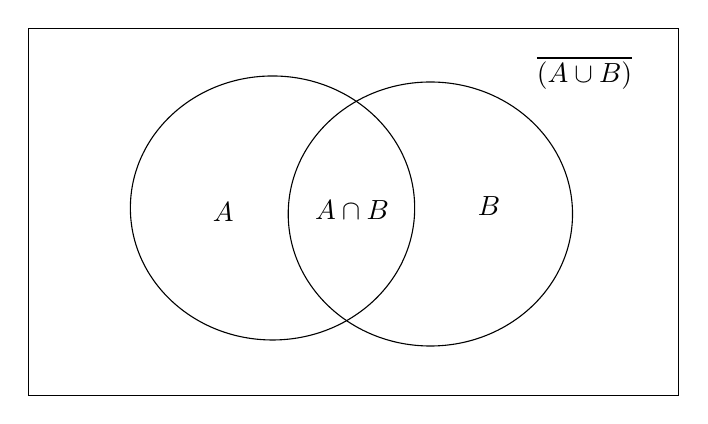
\begin{tikzpicture}[x=0.75pt,y=0.75pt,yscale=-1,xscale=1]
%uncomment if require: \path (0,228.46875); %set diagram left start at 0, and has height of 228.46875

\draw    (153, 22.47) rectangle (466.5, 199.47)   ;
\draw    (270.7, 109.07) circle [x radius= 68.49, y radius= 63.6]  ;
\draw    (346.75, 111.97) circle [x radius= 68.49, y radius= 63.6]  ;

\draw (247,111) node   {$A$};
\draw (375,108) node   {$B$};
\draw (309,110) node   {$A\cap B$};
\draw (421,44) node   {$\overline{\left(A\cup B\right)}$};
\end{tikzpicture}
\end{center}


\subsection{Classical Definition of Probability}

In an experiment with outcomes given by the set $\Omega$, the outcomes associated with event $A$ is a subset of $\Omega$ (ie. $A \subseteq \Omega$). Suppose we have a way to count these outcomes. Let $\left|\Omega\right|$ be the number of outcomes in $\Omega$, and similarly let $\left|A\right|$ be the number of outcomes in $A$. Then by the classical definition of probability, the probability of event $A$, denoted $\operatorname{Pr}\left(A\right)$, is
\begin{equation}
\operatorname{Pr}\left(A\right) = \dfrac{\left|A\right|}{\left|\Omega\right|}
\end{equation}

This means that probabilities are always between $0$ and $1$ (inclusive). We can interpret this probability by saying if we were able to conduct an infinite number of experiments, then the proportion of experiments which resulted in the occurrence of $A$ would be $\operatorname{Pr}\left(A\right)$.

\subsection{Addition Rule of Probability}

The probability of the intersection of $A$ and $B$ is written $\operatorname{Pr}\left(A \cap B\right)$, or alternatively may be denoted $\operatorname{Pr}\left(A, B\right)$. To obtain the probability of the union between $A$ and $B$, we have the formula (called the addition rule of probability):
\begin{equation}
\operatorname{Pr}\left(A \cup B\right) = \operatorname{Pr}\left(A\right) + \operatorname{Pr}\left( B\right) - \operatorname{Pr}\left(A \cap B\right) 
\end{equation}

\subsection{Complementary Probabilities}

The complementary probability of $\operatorname{Pr}\left(A\right)$ is denoted $\operatorname{Pr}\left(\overline{A}\right)$. We have that
\begin{equation}
\operatorname{Pr}\left(\overline{A}\right) = 1 - \operatorname{Pr}\left(A\right)
\end{equation}

\subsection{Mutual Exclusivity}

Events $A$ and $B$ are mutually exclusive if they cannot both happen together. That means
\begin{equation}
\operatorname{Pr}\left(A \cap B \right) = 0
\end{equation}
Hence the addition rule of probability in the case of mutual exclusivity simplifies to
\begin{equation}
\operatorname{Pr}\left(A \cup B\right) = \operatorname{Pr}\left(A\right) + \operatorname{Pr}\left( B\right)
\end{equation}

\subsection{Conditional Probability}

The probability of event $A$ occurring given event $B$ has occurred is denoted by $\operatorname{Pr}\left(A\middle|B\right)$ and is known as a conditional probability. The conditional probability can be calculated by
\begin{equation}
\operatorname{Pr}\left(A\middle|B\right) = \dfrac{\operatorname{Pr}\left(A \cap B\right)}{\operatorname{Pr}\left(B\right)}
\end{equation}
The term $\operatorname{Pr}\left(B\right)$ can be thought of as a `normalising constant' for $\operatorname{Pr}\left(A \cap B\right)$, as we only want to consider the space of outcomes where $B$ has occurred.

\subsection{Chain Rule of Probability}

Given the conditional probability $\operatorname{Pr}\left(A\middle|B\right)$ and the marginal probability $\operatorname{Pr}\left(B\right)$, the chain rule of probability says that the `joint' probability $\operatorname{Pr}\left(A\cap B\right)$ is equal to
\begin{equation}
\operatorname{Pr}\left(A\cap B\right) = \operatorname{Pr}\left(A\middle|B\right)\operatorname{Pr}\left(B\right)
\end{equation}

\subsection{Law of Total Probability}

The law of total probability gives a way to write the probability of an event $B$ in terms of its conditional probabilities, using the chain rule of probability. For events $A$ and $B$, the law of total probability says that
\begin{equation}
\operatorname{Pr}\left(B\right) = \operatorname{Pr}\left(A\right)\operatorname{Pr}\left(B\middle|A\right) + \operatorname{Pr}\left(\overline{A}\right)\operatorname{Pr}\left(B\middle|\overline{A}\right)
\end{equation}

\subsubsection{Probability Tree Diagrams}
A probability tree diagram for two events $A$, $B$ is given below.
\begin{center}
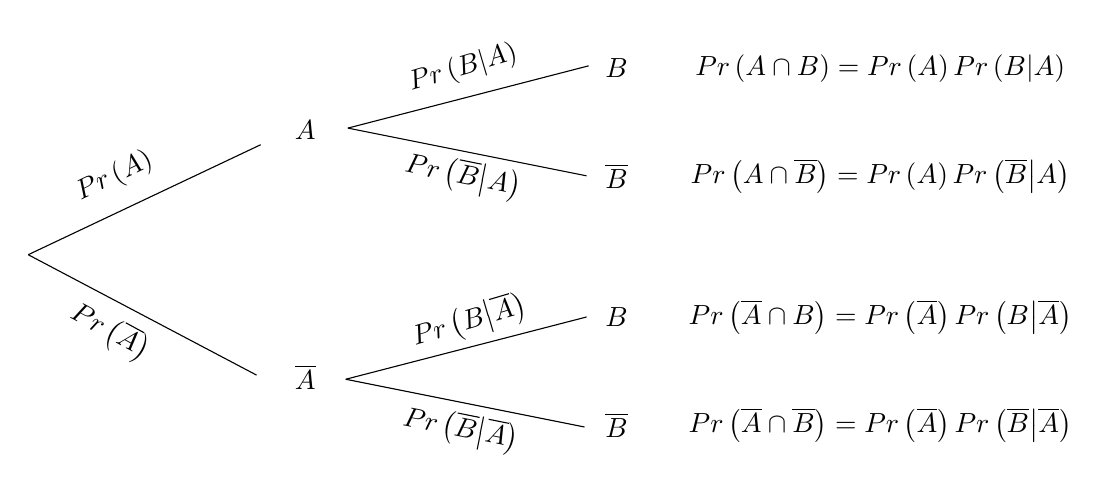
\begin{tikzpicture}[x=0.75pt,y=0.75pt,yscale=-1,xscale=1]
%uncomment if require: \path (0,228.84375); %set diagram left start at 0, and has height of 228.84375
\draw    (119.5,117.84) -- (231.5,64.84) ;

\draw    (119.5,117.84) -- (229.5,175.84) ;

\draw    (273.5,56.84) -- (389.5,26.84) ;

\draw    (273.5,56.84) -- (388.5,79.84) ;

\draw    (272.5,177.84) -- (388.5,147.84) ;
\draw    (272.5,177.84) -- (387.5,200.84) ;

\draw (253,58) node   {$A$};
\draw (253,177) node   {$\overline{A}$};
\draw (161,80) node [rotate=-334.26]  {$\operatorname{Pr}\left(A\right)$};
\draw (159,155) node [rotate=-28.56]  {$\operatorname{Pr}\left(\overline{A}\right)$};
\draw (403,200) node   {$\overline{B}$};
\draw (403,148) node   {$B$};
\draw (403,80) node   {$\overline{B}$};
\draw (403,28) node   {$B$};
\draw (329,28) node [rotate=-343.54]  {$\operatorname{Pr}\left(B\middle|A\right)$};
\draw (329,80) node [rotate=-11.43]  {$\operatorname{Pr}\left(\overline{B}\middle|A\right)$};
\draw (332,150) node [rotate=-343.54]  {$\operatorname{Pr}\left(B\middle|\overline{A}\right)$};
\draw (328,202) node [rotate=-11.43]  {$\operatorname{Pr}\left(\overline{B}\middle|\overline{A}\right)$};
\draw (530,28) node   {$\operatorname{Pr}\left(A\cap B\right) = \operatorname{Pr}\left(A\right)\operatorname{Pr}\left(B\middle|A\right)$};
\draw (530,80) node   {$\operatorname{Pr}\left(A\cap \overline{B}\right) = \operatorname{Pr}\left(A\right)\operatorname{Pr}\left(\overline{B}\middle|A\right)$};
\draw (530,148) node   {$\operatorname{Pr}\left(\overline{A}\cap B\right) = \operatorname{Pr}\left(\overline{A}\right)\operatorname{Pr}\left(B\middle|\overline{A}\right)$};
\draw (530,200) node   {$\operatorname{Pr}\left(\overline{A}\cap \overline{B}\right) = \operatorname{Pr}\left(\overline{A}\right)\operatorname{Pr}\left(\overline{B}\middle|\overline{A}\right)$};
\end{tikzpicture}

\end{center}
Probability tree diagrams allow for the law of total probability to be visualised. One can think of obtaining $\operatorname{Pr}\left(B\right)$ across all branches to the tree to find the joint probabilities, then summing over the probabilities which are favourable to event $B$.

\subsection{Bayes' Theorem}

By definitions of conditional probability, we have for two events $A$, $B$:
\begin{gather}
\operatorname{Pr}\left(A\middle|B\right) = \dfrac{\operatorname{Pr}\left(A\cap B\right)}{\operatorname{Pr}\left(B\right)} \\
\operatorname{Pr}\left(B\middle|A\right) = \dfrac{\operatorname{Pr}\left(A\cap B\right)}{\operatorname{Pr}\left(A\right)}
\end{gather}
Rearranging both gives
\begin{gather}
\operatorname{Pr}\left(A\cap B\right) = \operatorname{Pr}\left(A\middle|B\right)\operatorname{Pr}\left(B\right) \\
\operatorname{Pr}\left(A\cap B\right) = \operatorname{Pr}\left(B\middle|A\right)\operatorname{Pr}\left(A\right)
\end{gather}
Then equating them gives Bayes' theorem
\begin{gather}
\operatorname{Pr}\left(A\middle|B\right)\operatorname{Pr}\left(B\right) = \operatorname{Pr}\left(B\middle|A\right)\operatorname{Pr}\left(A\right) \\
\operatorname{Pr}\left(A\middle|B\right) = \dfrac{\operatorname{Pr}\left(B\middle|A\right)\operatorname{Pr}\left(A\right)}{\operatorname{Pr}\left(B\right)}
\end{gather}
where $\operatorname{Pr}\left(A\middle|B\right)$ is known as the posterior probability, $\operatorname{Pr}\left(A\right)$ is known as the prior probability, $\operatorname{Pr}\left(B\middle|A\right)$ is known as the likelihood and $\operatorname{Pr}\left(B\right)$ is known as the marginal likelihood.

\subsection{DeMorgan's Laws}

DeMorgan's laws can be arrived at via some logical postulates.
\begin{itemize}
\item The event of $A$ or $B$ not happening is the same as neither $A$ happening nor $B$ happening.
\item The event that $A$ and $B$ both do not happen is the same as either $A$ not happening or $B$ not happening. 
\end{itemize}
This can be written down using set notation:
\begin{gather}
\overline{A \cup B} = \overline{A} \cap \overline{B} \\
\overline{A \cap B} = \overline{A} \cup \overline{B}
\end{gather}
And in terms of probability:
\begin{gather}
\operatorname{Pr}\left(\overline{A \cup B}\right) = \operatorname{Pr}\left(\overline{A} \cap \overline{B}\right) \\
\operatorname{Pr}\left(\overline{A \cap B}\right) = \operatorname{Pr}\left(\overline{A} \cup \overline{B}\right)
\end{gather}
Or by using complements:
\begin{gather}
1 - \operatorname{Pr}\left(A \cup B\right) = \operatorname{Pr}\left(\overline{A} \cap \overline{B}\right) \\
1 - \operatorname{Pr}\left(A \cap B\right) = \operatorname{Pr}\left(\overline{A} \cup \overline{B}\right)
\end{gather}

\section{Introductory Combinatorics}

In the context of probability, combinatorics allows us to count the number of outcomes, relating to both the number of outcomes in an experiment, and the number of outcomes favourable to an event.

\subsection{Arrangements}

\subsubsection{Homogeneous Sequences}
Consider a sequence of `symbols' that can be made up of an `alphabet' of size $n$. Then for a sequence of length $m$, there are $n^{m}$ different ways to form such sequences without restriction.

\subsubsection{Inhomogeneous Sequences}
Consider a sequence of symbols where the $j$\textsuperscript{th} symbol in the sequences comes from an alphabet of size $n_{j}$. Then for a sequence of length $m$, there are $n_{1}\times n_{2}\times\dots\times n_{m}$ different ways to form such sequences without restriction. This can be used to calculate the total number of outcomes at the end of a probability tree for example.

\subsubsection{Arrangements in a Line}
Consider the number of different ways to order $n$ different symbols. There are $n$ possibilities for the first symbol, $n - 1$ possibilities for the second symbol, etc. Hence there are
\begin{equation}
n\times\left(n - 1\right)\times \dots\times 2\times 1 = n!
\end{equation}
different ways.

\subsubsection{Arrangements in a Circle}

Consider the number of different ways to arrange $n$ distinct objects in a circle (where it only matters which object is next to which). The first object can be placed in any arbitrary position. There are $n - 1$ possibilities for the second object placed next to the first object, and $n - 2$ possibilities for the third object places next to the second object, etc. Hence there are
\begin{equation}
\left(n - 1\right)\times \dots\times 2\times 1 = \left(n - 1\right)!
\end{equation}
different ways. Note that if it did matter which position in the circle each object was placed, the number of arrangements becomes the same as the number of arrangements in a line.

\subsection{Permutations}

Consider the number of different ways to pick $k$ objects from a pool of $n$ distinct objects, where the order in which they are picked matters. There are $n$ possibilities for the first pick, $n - 1$ possibilities for the second pick, up to $n - k + 1$ possibilities for the $k$\textsuperscript{th} pick. Hence there are
\begin{equation}
n\times\left(n - 1\right)\times \dots\times \left(n - k + 1\right) = \dfrac{n!}{\left(n - k\right)!}
\end{equation}
different ways. This is called the number of permutations, and may be denoted as $\mathstrut^{n}\mathsf{P}_{k}$. This also gives the number of different ways to arrange $k$ distinct objects among $\left(n - k\right)$ other homogeneous objects in a line (ie. there are $n$ objects total). This is because there are $n$ possible locations for the first object, up to $n - k + 1$ possible locations for the $k$\textsuperscript{th} object.

\subsubsection{Permutations in a Circle}

With $n$ total objects, consider the number of different ways to arrange $k$ distinct objects among $\left(n - k\right)$ other homogeneous objects in a circle (where it only matters which object is next to which). The first object can be placed in any arbitrary position. There are $n - 1$ possible positions for where the second object can be placed relative to first object, $n - 2$ possible positions for where the third object can be placed relative to first object, up to $n - k + 1$ possible positions for where the $k$\textsuperscript{th} object can be placed relative to first object. Hence there are
\begin{equation}
\left(n - 1\right)\times \dots\times \left(n - k + 1\right) = \dfrac{\left(n - 1\right)!}{\left(n - k\right)!}
\end{equation}
different ways. Note that we can arrive at this number by counting $\mathstrut^{n}\mathsf{P}_{k}$ permutations in a circle where absolute position 
does matter (equivalent to permutations in a line), but then dividing by the possible number of rotations in a circle without affecting relative positions, which is $n$.

\subsection{Combinations}

\subsubsection{Binomial Coefficient}

Consider the number of different ways to pick $k$ objects from a pool of $n$ distinct objects, where the order in which they are picked does not matter (ie. it only matters which group of $k$ are picked). We know that there are $\mathstrut^{n}\mathsf{P}_{k}$ different ways to pick $k$ objects when order does matter, but this number counts all the $k!$ different ways for every possible grouping of $k$ objects from the pool. So dividing the number of permutations by $k!$ gives
\begin{equation}
\dfrac{\mathstrut^{n}\mathsf{P}_{k}}{k!} = \dfrac{n!}{k!\left(n - k\right)!}
\end{equation}
which is the number of different groups of $k$ can be picked from $n$ distinct objects. This is known as the binomial coefficient, and denoted $\mathstrut^{n}\mathsf{C}_{k}$, which may also be read as "$n$ choose $k$". It is also sometimes denoted
\begin{equation}
\mathstrut^{n}\mathsf{C}_{k} = \binom{n}{k}
\end{equation}
This number can also be thought of as the number of different ways to arrange $k$ homogeneous objects among $\left(n - k\right)$ other homogeneous objects in a line. Note that the following properties hold for the binomial coefficient:
\begin{equation}
\mathstrut^{n}\mathsf{C}_{k} = \mathstrut^{n}\mathsf{C}_{n - k}
\end{equation}
which says that asking for the number of ways to choose $k$ from $n$ is no different to asking for the number of ways to choose $n - k$ from $n$. Also
\begin{equation}
\mathstrut^{n}\mathsf{C}_{0} + \mathstrut^{n}\mathsf{C}_{1} + \dots + \mathstrut^{n}\mathsf{C}_{n} = 2^{n}
\end{equation}
since there are $2^{n}$ different binary sequences of length $n$, and the above sum exhaustively enumerates through all combinations of binary sequences from when there are zero `$1$'s up to $n$ `$1$'s.

\subsubsection{Multinomial Coefficient}

As a generalisation to the binomial coefficient, suppose there are $n$ objects and $m$ different groups, with the numbers of homogeneous objects in each group given by $k_{1}, k_{2}, \dots, k_{m}$ and so we have
\begin{equation}
k_{1} + k_{2} + \dots + k_{m} = n
\end{equation}
To derive the number of different ways these objects can be arranged, first consider the number of ways to arrange only the first group (which has $k_{1}$ members), without regard for the other groups (call it the `remainder' group). By the binomial coefficient, there are
\begin{equation}
\mathstrut^{n}\mathsf{C}_{k_{1}} = \dfrac{n!}{k_{1}!\left(n - k_{1}\right)!}
\end{equation}
ways. Then for every one of these arrangements, there are $\mathstrut^{n - k_{1}}\mathsf{C}_{k_{2}}$ ways to arrange members of group $2$ among the remainder. Hence there are
\begin{equation}
\mathstrut^{n}\mathsf{C}_{k_{1}}\times\mathstrut^{n - k_{1}}\mathsf{C}_{k_{2}} = \dfrac{n!}{k_{1}!\left(n - k_{1}\right)!}\times\dfrac{\left(n - k_{1}\right)!}{k_{2}!\left(n - k_{1} - k_{2}\right)!}
\end{equation}
different ways to arrange objects in groups $1$ and $2$, without regard for the others. By continuing this process of induction, we find that
\begin{multline}
\mathstrut^{n}\mathsf{C}_{k_{1}}\times\mathstrut^{n - k_{1}}\mathsf{C}_{k_{2}}\times\dots\times\mathstrut^{n - k_{1} - \dots - k_{m - 1}}\mathsf{C}_{k_{m}} = \dfrac{n!}{k_{1}!\left(n - k_{1}\right)!}\times\dfrac{\left(n - k_{1}\right)!}{k_{2}!\left(n - k_{1} - k_{2}\right)!}\times\dots \\
\times \dfrac{\left(n - k_{1} - \dots - k_{m - 2}\right)!}{k_{m - 1}!\left(n - k_{1} - \dots - k_{m - 1}\right)!}\times\dfrac{\left(n - k_{1} - \dots - k_{m - 1}\right)!}{k_{m}!0!}
\end{multline}
gives the number of different ways to arrange all objects in all groups. By cancellation of terms, the multinomial coefficient can be denoted as
\begin{equation}
\binom{n}{k_{1}, \dots, k_{m}} = \dfrac{n!}{k_{1}!k_{2}!\dots k_{m}!}
\end{equation}
This number can also be thought of as the number of ways of depositing $n$ distinct objects into $m$ bins, where the $j$\textsuperscript{th} bin requires $k_{j}$ objects.

\subsubsection{Combinations in a Circle}

With $n$ total objects, consider the number of different ways to arrange $k$ homogeneous objects among $\left(n - k\right)$ other homogeneous objects in a circle (where it only matters which object is next to which). Like with arrangements and permutations in a circle, we can find this number by dividing the total number of combinations in a line by the number of possible rotations without affecting relative position, which is $n$. This gives
\begin{equation}
\dfrac{\mathstrut^{n}\mathsf{C}_{k}}{n} = \dfrac{\left(n - 1\right)!}{k!\left(n - k\right)!}
\end{equation}

\section{Probability Distributions}

\subsection{Random Variables}

Random variables are variables which are determined as a result of a random experiment, ie. they are not fixed and will depend on the outcome of the random experiment. This is in contrast to `deterministic' variables, which are always fixed regardless of the outcome. Deterministic variables can even be thought to be a special case of random variables, which are determined at the end of the random experiment but always take on the same value. \\

The value of a random variable after the experiment has occurred is said to have been `realised'.

\subsubsection{Degenerate Random Variables}

A degenerate random variable takes on a single value with probability $1$, and thus can be regarded as a deterministic variable.

\subsubsection{Binary Random Variables}

Binary random variables are random variables which can take on either of two possible values, usually chosen to be $0$ and $1$.

\subsubsection{Indicator Random Variables}

An indicator random variable for an event $A$ is a binary random variable that takes on the value of $1$ if $A$ occurred, and $0$ if $A$ did not occur. An indicator for $A$ can be denoted by $\mathbb{I}_{A}$.

\subsubsection{Simple Random Variables}

A simple random variable is a weighted sum of indicator random variables for mutually exclusive events. Suppose $A_{1}, \dots, A_{n}$ are $n$ mutually exclusive events. Then a simple random variable $X$ is
\begin{equation}
X = \sum_{i = 1}^{n}a_{i}\mathbb{I}_{A_{i}}
\end{equation}
where $a_{1}, \dots, a_{n}$ are the weights.

\subsection{Distribution Functions}

The possible values which a random variable can take, as well as probabilities of random variables taking on certain values, is represented using a distribution function.

\subsubsection{Discrete Distributions}

For a random variable $X$ that takes on discrete values (eg. $0, 1, 2, \dots$), the probability mass function describes the probability of $X$ being equal to a particular value, denoted $\operatorname{Pr}\left(X = x\right)$. Note that for random experiments with discrete outcomes which do not explicitly result in the realisation of a random variable, a discrete random variable can still be defined by assigning each outcome to the set of integers (and if an integer $x$ is not assigned to any outcome, this simply means $\operatorname{Pr}\left(X = x\right) = 0$). In this way, a probability mass function can still be defined for any random experiment with discrete outcomes. A probability mass function satisfies the following properties:
\begin{equation}
\sum_{x=-\infty}^{\infty}\operatorname{Pr}\left(X = x\right) = 1
\end{equation}
and
\begin{equation}
0 \leq \operatorname{Pr}\left(X = x\right) \leq 1
\end{equation}
for all integers $x$.

\subsubsection{Continuous Distributions}

In some random experiments, a random variable can take on a continuum of values (eg. $\left[0, 1\right]$ or $\left(-\infty, \infty\right)$). These are called continuous random variables. A continuous random variable $X$ has a probability density function, denoted $f_{X}\left(x\right)$. Integrating this function over regions gives the probability that $X$ will lie in that region. For example, the probability that $a \leq X \leq b$ is given by
\begin{equation}
\operatorname{Pr}\left(a \leq X \leq b\right) = \int_{a}^{b}f_{X}\left(x\right)dx
\end{equation}
Note that is does not matter if this is integrated with open intervals or closed intervals. Hence for a continuous random variable, $\operatorname{Pr}\left(a \leq X \leq b\right) = \operatorname{Pr}\left(a < X < B\right)$. Also, the probability that $X$ takes on any one particular value is zero, ie. $\operatorname{Pr}\left(X = x\right) = 0$. That means it only makes sense to talk about $X$ lying within regions, rather than for specific points. A probability density function satisfies the following properties:
\begin{equation}
\int_{-\infty}^{\infty}f_{X}\left(x\right)dx = 1
\end{equation}
and
\begin{equation}
f_{X}\left(x\right) \geq 0
\end{equation}
for all $x\in\left(-\infty, \infty\right)$. Note that unlike probability masses, probability densities are allowed to be greater than $1$.

\subsubsection{Cumulative Distributions}

A cumulative distribution function $F_{X}\left(x\right)$ for a random variable $X$ is defined as a function for the `cumulative' probability up to $x$:
\begin{equation}
F_{X}\left(x\right) = \operatorname{Pr}\left(X \leq x\right)
\end{equation}
Thus if $X$ is a discrete random variable, then the relation between the cumulative distribution function and the probability mass function is given by
\begin{equation}
F_{X}\left(a\right) = \sum_{x = -\infty}^{a}\operatorname{Pr}\left(X = x\right)
\end{equation}
Whereas if $X$ is a continuous random variable, then the relation between the cumulative distribution function and the probability density function is given by
\begin{equation}
F_{X}\left(a\right) = \int_{-\infty}^{a}f_{X}\left(x\right)dx
\end{equation}
The cumulative distribution satisfies the following properties:
\begin{equation}
0 \leq F_{X}\left(x\right) \leq 1
\end{equation}
for all $x$, and
\begin{gather}
\lim_{x\to -\infty}F_{X}\left(x\right) = 0 \\
\lim_{x\to \infty}F_{X}\left(x\right) = 1
\end{gather}
Furthermore, the probability density function can be obtained from the cumulative density function by
\begin{equation}
f_{X}\left(x\right) = \dfrac{dF_{X}\left(x\right)}{dx}
\end{equation}
(wherever the cumulative density function is differentiable) and if given the probability density function, then
\begin{equation}
F_{X}\left(x\right) = \int f_{X}\left(x\right)dx
\end{equation}
with a constant of integration such that $\lim_{x\to \infty}F_{X}\left(x\right) = 1$. The cumulative distribution function is always non-decreasing, since probabilities and densities are non-negative. If $X$ is discrete, then $F_{X}\left(x\right)$ will have `jumps', but is by convention treated as right-continuous, to keep up with the definition $F_{X}\left(x\right) = \operatorname{Pr}\left(X \leq x\right)$.

\subsubsection{Quantile Function}

The quantile function can roughly be thought of as the inverse of the cumulative distribution function. However, the cumulative distribution may not always be invertible. In that case, we can define the quantile function $Q\left(p\right)$ which takes $p\in\left[0, 1\right]$ as the smallest $x$ such that $F_{X}\left(x\right) = \operatorname{Pr}\left(X \leq x\right) \geq p$. More formally, we can write this as an infimum:
\begin{equation}
Q\left(p\right) = \inf\left\{x: F_{X}\left(x\right) \geq p\right\}
\end{equation}
The quantile function can also be denoted $F^{-1}\left(p\right)$. Choosing this definition for the quantile function means that the following conditions:
\begin{gather}
p \leq F\left(c\right) \\
F^{-1}\left(p\right) \leq c
\end{gather} 
are equivalent. To show this in the forward direction starting with $p \leq F\left(c\right)$, let
\begin{align}
x^{*} &= \inf\left\{x: F\left(x\right) \geq p\right\} \\
&= F^{-1}\left(p\right)
\end{align}
Then since the cumulative distribution is non-decreasing, $F\left(x^{*}\right) = \inf\left\{F\left(x\right): F\left(x\right) \geq p\right\}$ and from the condition $p \leq F\left(c\right)$ this must mean $F\left(x^{*}\right) \leq F\left(c\right)$. Apply the non-decreasing property again to obtain $x^{*} \leq c$, and therefore by definition of $x^{*} = F^{-1}\left(p\right)$:
\begin{equation}
F^{-1}\left(p\right) \leq c
\end{equation}
To show the reverse beginning with $F^{-1}\left(p\right) \leq c$, define yet again $x^{*} = \inf\left\{x: F\left(x\right) \geq p\right\}$ so that $F\left(x^{*}\right) \geq p$ and $x^{*} = F^{-1}\left(p\right) \leq c$. Using the non-decreasing property of $F\left(\cdot\right)$, this implies $F\left(x^{*}\right) \leq F\left(c\right)$ hence:
\begin{equation}
p \leq F\left(c\right)
\end{equation}
Since by convention the cumulative distribution function is right-continuous, then this this definition ensures the quantile function will be left-continuous.

\subsection{Joint Distributions}

Consider a random experiment which produces two random variables, $X$ and $Y$. If these random variables are discrete (taking on integer values), we can express a joint probability mass function over all combinations of $X$ and $Y$, given by $\operatorname{Pr}\left(X = x, Y = y\right)$. This joint distribution has the property that
\begin{equation}
\sum_{x = -\infty}^{\infty}\sum_{y = -\infty}^{\infty}\operatorname{Pr}\left(X = x, Y = y\right) = 1
\end{equation}
We call $\operatorname{Pr}\left(X = x\right)$ and $\operatorname{Pr}\left(Y = y\right)$ the marginal distributions, which can be calculated from the joint distribution by a summation:
\begin{gather}
\operatorname{Pr}\left(X = x\right) = \sum_{y = -\infty}^{\infty}\operatorname{Pr}\left(X = x, Y = y\right) \\
\operatorname{Pr}\left(Y = y\right) = \sum_{x = -\infty}^{\infty}\operatorname{Pr}\left(X = x, Y = y\right)
\end{gather}
Analogously, if $X$ and $Y$ are continuous, then there exists a joint density function denoted $f_{XY}\left(x, y\right)$ with the relation
\begin{equation}
\int_{-\infty}^{\infty}\int_{-\infty}^{\infty}f_{XY}\left(x, y\right)dxdy = 1
\end{equation}
and the marginal densities $f_{X}\left(x\right)$, $f_{Y}\left(y\right)$ given by the integrals
\begin{gather}
f_{X}\left(x\right) = \int_{-\infty}^{\infty}f_{XY}\left(x, y\right)dy \\
f_{Y}\left(y\right) = \int_{-\infty}^{\infty}f_{XY}\left(x, y\right)dx
\end{gather}
Note that while it is possible to obtain marginal distributions from the joint distribution (via the process known as `marginalisation'), it is generally not possible to obtain the joint distribution from the marginal distributions (with the exception of special cases), as there may be more than one joint distribution while would yield those marginal distributions.

\subsection{Conditional Distributions}

By the definition of the conditional probability, we know (for discrete $X$ and $Y$):
\begin{equation}
\operatorname{Pr}\left(X = x\middle|Y = y\right) = \dfrac{\operatorname{Pr}\left(X = x, Y = y\right)}{\operatorname{Pr}\left(Y = y\right)}
\end{equation}
this is known as the conditional distribution of $X$ given $Y$, and is itself a probability mass function which is dependent on the value of $Y$. Notice that it is the quotient between the joint distribution of $X, Y$ and the marginal distribution of $Y$, and is defined only when $\operatorname{Pr}\left(Y = y\right) > 0$, otherwise we can presume $\operatorname{Pr}\left(X = x\middle|Y = y\right) = 0$. Likewise, the conditional distribution of $Y$ given $X$ is
\begin{equation}
\operatorname{Pr}\left(Y = y\middle|X = x\right) = \dfrac{\operatorname{Pr}\left(X = x, Y = y\right)}{\operatorname{Pr}\left(X = x\right)}
\end{equation}
Using the chain rule of probability, we can relate the marginal distribution of $X$ to the conditional distribution of $X$ given $Y$ by
\begin{align}
\operatorname{Pr}\left(X = x\right) &= \sum_{y = -\infty}^{\infty}\operatorname{Pr}\left(X = x, Y = y\right)\\
&= \sum_{\left\{y: \operatorname{Pr}\left(Y = y\right) > 0\right\}}\operatorname{Pr}\left(X = x\middle|Y = y\right)\operatorname{Pr}\left(Y = y\right)
\end{align}
We can also show that the conditional distribution $\operatorname{Pr}\left(X = x\middle|Y = y\right)$ is a proper distribution (summing over $x$ to $1$) for any given $y$:
\begin{align}
\sum_{x = -\infty}^{\infty}\operatorname{Pr}\left(X = x\middle|Y = y\right) &= \sum_{x = -\infty}^{\infty}\dfrac{\operatorname{Pr}\left(X = x, Y = y\right)}{\operatorname{Pr}\left(Y = y\right)} \\
&= \dfrac{1}{\operatorname{Pr}\left(Y = y\right)}\sum_{x = -\infty}^{\infty}\operatorname{Pr}\left(X = x, Y = y\right) \\
&= \dfrac{\operatorname{Pr}\left(Y = y\right)}{\operatorname{Pr}\left(Y = y\right)} \\
&= 1
\end{align}
If $X$ and $Y$ are continuous, then there exists conditional densities $f_{X|Y}\left(x\middle|Y = y\right)$ and $f_{Y|X}\left(y\middle|X = x\right)$. These are similarly defined by
\begin{gather}
f_{X|Y}\left(x\middle|Y = y\right) = \dfrac{f_{XY}\left(x, y\right)}{f_{Y}\left(y\right)} \\
f_{Y|X}\left(y\middle|X = x\right) = \dfrac{f_{XY}\left(x, y\right)}{f_{X}\left(x\right)} 
\end{gather}
where we can show similar properties as with discrete distributions hold:
\begin{align}
f_{X}\left(x\right) &= \int_{-\infty}^{\infty}f_{XY}\left(x, y\right)dy \\
&= \int_{\left\{y: f_{Y}\left(y\right) > 0\right\}}f_{X|Y}\left(x\middle|Y = y\right)f_{Y}\left(y\right)dy
\end{align}
and
\begin{align}
\int_{-\infty}^{\infty}f_{X|Y}\left(x\middle|Y = y\right)dx &= \int_{-\infty}^{\infty}\dfrac{f_{XY}\left(x, y\right)}{f_{Y}\left(y\right)}dx \\
&= \dfrac{1}{f_{Y}\left(y\right)}\int_{-\infty}^{\infty}f_{XY}\left(x, y\right)dx \\
&= \dfrac{f_{Y}\left(y\right)}{f_{Y}\left(y\right)} \\
&= 1
\end{align}

\subsubsection{Conditional Random Variables}

A `conditional random variable' denoted $X|Y$ can be informally defined as the random variable which has its own distribution function the conditional distribution of $X$ given $Y$.

\subsection{Support of a Distribution}

The support of a distribution for a random variable is the set of values for which the probability density function (or probability mass function, in the case of discrete random variables) is non-zero. For example, we can denote the support of a discrete random variable $X$ as
\begin{equation}
\mathcal{X} := \left\{x: \operatorname{Pr}\left(X = x\right) > 0\right\}
\end{equation}

\section{Expectation}

The expectation (or expected value, or mean) of a random variable can be thought about in several ways:
\begin{itemize}
\item The average realisation of the random variable over an infinite number of trials.
\item The `center of mass' of the probability distribution.
\end{itemize}
The expected value of a random variable $X$ is a constant denoted $\mathbb{E}\left[X\right]$ and for a discrete random variable may be calculated as
\begin{equation}
\mathbb{E}\left[X\right] = \sum_{x = -\infty}^{\infty}x\operatorname{Pr}\left(X = x\right)
\end{equation}
If $X$ is a continuous random variable, then the expectation is calculated by
\begin{equation}
\mathbb{E}\left[X\right] = \int_{-\infty}^{\infty}xf_{X}\left(x\right)dx
\end{equation}
Expectations of functions of random variables (which are also random variables) are readily calculable, for example some with $g\left(X\right)$, the so-called Law of the unconscious statistician is given by:
\begin{equation}
\mathbb{E}\left[g\left(X\right)\right] = \int_{-\infty}^{\infty}g\left(x\right)f_{X}\left(x\right)dx
\end{equation}
If an experiment results in two (continuous) random variables $X$ and $Y$, we can also take the expectation of some function of the two random variables $g\left(X, Y\right)$ by
\begin{equation}
\mathbb{E}\left[g\left(X, Y\right)\right] = \int_{-\infty}^{\infty}\int_{-\infty}^{\infty}g\left(x, y\right)f_{XY}\left(x, y\right)dxdy
\end{equation}
and analogously for discrete random variables. Sometimes, particularly when there are multiple random variables present, an expectation may be taken with respect to a random variable, which expresses which marginal distribution to sum/integrate over. For example, with a continuous random variable $X$ and a function $g\left(X\right)$,the expectation of $g\left(X\right)$ with respect to $X$ is denoted with $\mathbb{E}_{X}\left[g\left(X\right)\right]$, and defined like above as
\begin{equation}
\mathbb{E}_{X}\left[g\left(X\right)\right] = \int_{-\infty}^{\infty}g\left(x\right)f_{X}\left(x\right)dx
\end{equation}
This is more for emphasis and clarity rather than any technical difference, since $g\left(X\right)$ may be written using another symbol which does not make the connection with $X$ explicit.

\subsection{Linearity of Expectation}

Consider two random variables $X$, $Y$ and two constants $a$, $b$. The expectation of $aX + bY$ (supposing $X$ and $Y$ are discrete) is written as
\begin{align}
\mathbb{E}\left[aX + bY\right] &= \sum_{x}\sum_{y}\left(ax + by\right)\operatorname{Pr}\left(X = x, Y = y\right) \\
&= a\sum_{x}\sum_{y}x\operatorname{Pr}\left(X = x, Y = y\right) + b\sum_{x}\sum_{y}y\operatorname{Pr}\left(X = x, Y = y\right) \\
&= a\sum_{x}x\sum_{y}\operatorname{Pr}\left(X = x, Y = y\right) + b\sum_{y}y\sum_{x}\operatorname{Pr}\left(X = x, Y = y\right) \\
&= a\sum_{x}x\operatorname{Pr}\left(X = x\right) + b\sum_{y}y\operatorname{Pr}\left(Y = y\right) \\
&= a\mathbb{E}\left[X\right] + b\mathbb{E}\left[Y\right]
\end{align}
This analogously holds for continuous $X$ and $Y$. Since sums and integrals are linear operators, and the expectation is defined either in terms of sums or integrals, this gives the property known as the linearity of expectation.

\subsection{Conditional Expectation}

The conditional expectation of $X$ given $Y$ is denoted $\mathbb{E}\left[X\middle|Y\right]$, and may be interpreted in two ways:
\begin{itemize}
\item Given a particular value of $Y = y$, the conditional expectation $\mathbb{E}\left[X\middle|Y = y\right]$ is the average of $X$ over all events where $Y = y$. It may be calculated by taking the expectation of the conditional distribution of $X$ given $Y$, ie. for discrete random variables
\begin{equation}
\mathbb{E}\left[X\middle|Y = y\right] = \sum_{x}x\operatorname{Pr}\left(X = x\middle|Y = y\right)
\end{equation}
For continuous random variables,
\begin{equation}
\mathbb{E}\left[X\middle|Y = y\right] = \int_{-\infty}^{\infty}xf_{X|Y}\left(x\middle|Y = y\right)dx
\end{equation}
This form of the conditional expectation may be treated as a deterministic function in the realisation $y$.
\item The conditional expectation $\mathbb{E}\left[X\middle|Y\right]$ without being given a particular value of $Y$ is a random variable, because $Y$ is random. For discrete $X$ and $Y$, the random variable $\mathbb{E}\left[X\middle|Y\right]$ is defined to take on value $\mathbb{E}\left[X\middle|Y = y\right]$ with probability $\operatorname{Pr}\left(Y = y\right)$. For continuous $X$ and $Y$, the random variable $\mathbb{E}\left[X\middle|Y\right]$ has density $f_{X|Y}\left(x\middle|Y = y\right)$ at value $\mathbb{E}\left[X\middle|Y = y\right]$.
\end{itemize}
The conditional expectation of $X$ conditional on its own realisation $X = x$ becomes $x$, ie. $\mathbb{E}\left[X\middle|X = x\right] = x$, because given $X = x$, we expect that $X$ naturally can only be $x$. We can show this more formally (for the case of a discrete random variable $X$) by using the facts that $\operatorname{Pr}\left(X = x \middle| X = x\right) = 1$ and $\operatorname{Pr}\left(X = x' \middle| X = x\right) = 0$ when $x' \neq x$:
\begin{align}
\mathbb{E}\left[X\middle|X = x\right] &= \sum_{x'}x'\operatorname{Pr}\left(X = x' \middle| X = x\right) \\
&= x
\end{align}
It can then be reasoned that $\mathbb{E}\left[X\middle|X\right] = X$, because by the definition above $X$ is the random variable which takes on value $\mathbb{E}\left[X\middle|X = x\right] = x$ with probability $\operatorname{Pr}\left(X = x\right)$. Generalising this, we can say that for a function $f\left(\cdot\right)$, we have
\begin{equation}
\mathbb{E}\left[f\left(X\right)\middle|X = x\right] = f\left(x\right)
\end{equation}
and
\begin{equation}
\mathbb{E}\left[f\left(X\right)\middle|X\right] = f\left(X\right)
\end{equation}

\subsection{Law of Iterated Expectations}

The law of iterated expectations (also sometimes referred to the law of total expectation) states that the expectation of the random variable $\mathbb{E}\left[X\middle|Y\right]$ (over $Y$) is $\mathbb{E}\left[X\right]$. That is,
\begin{equation}
\mathbb{E}\left[\mathbb{E}\left[X\middle|Y\right]\right] = \mathbb{E}\left[X\right]
\end{equation}
Sometimes the law is written $\mathbb{E}_{Y}\left[\mathbb{E}_{X}\left[X\middle|Y\right]\right] = \mathbb{E}\left[X\right]$ to explicitly show which variables the expectations are taken with respect to. To prove the law for discrete random variables,
\begin{align}
\mathbb{E}\left[\mathbb{E}\left[X\middle|Y\right]\right] &= \sum_{y}\mathbb{E}\left[X\middle|Y = y\right]\operatorname{Pr}\left(Y = y\right) \\
&= \sum_{y}\sum_{x}x\operatorname{Pr}\left(X = x\middle|Y = y\right)\operatorname{Pr}\left(Y = y\right) \\
&= \sum_{y}\sum_{x}x\operatorname{Pr}\left(X = x, Y = y\right) \\
&= \mathbb{E}\left[X\right]
\end{align}
This is similarly shown for continuous random variables. The law of iterated expectations can also be extended to when there are more than two random variables. Some variations are:
\begin{gather}
\mathbb{E}\left[\mathbb{E}\left[X\middle|Y, Z\right]\right] = \mathbb{E}\left[X\right] \\
\mathbb{E}\left[\mathbb{E}\left[X\middle|Y, Z\right]\middle|Z\right] = \mathbb{E}\left[X\middle|Z\right]
\end{gather}
Note that it is necessary to condition the inner expectation $\mathbb{E}\left[X\middle|Y, Z\right]$ in the second equation to also be conditional on $Z$. This is because if we instead wrote $\mathbb{E}\left[\mathbb{E}\left[X\middle|Y\right]\middle|Z\right]$, the outer expectation means $Z$ is given, while the inner expectation means $Z$ is not given, so this will not be very clearly defined.

\subsection{Expectation of Indicator Random Variables}

Let $\mathbb{I}_{A}$ be an indicator random variable for event $A$. The expectation of $\mathbb{I}_{A}$ is the probability of $A$, as shown below.
\begin{align}
\mathbb{E}\left[\mathbb{I}_{A}\right] &= 0\times \operatorname{Pr}\left(\overline{A}\right) + 1\times \operatorname{Pr}\left(A\right) \\
&= \operatorname{Pr}\left(A\right)
\end{align}

\subsection{Expectations Using the Cumulative Distribution Function}

Let $X$ be a non-negative random variable with cumulative distribution function $F_{X}\left(x\right)$. Then the expectation of $X$ can be alternatively characterised using $F_{X}\left(x\right)$ by noting
\begin{align}
X &= \int_{0}^{X}1\cdot dx \\
&= \int_{0}^{\infty}\mathbb{I}_{X > x} dx
\end{align}
where $\mathbb{I}_{X > x}$ is the indicator random variable for the event $\left\{X > x\right\}$. Hence
\begin{align}
\mathbb{E}\left[X\right] &= \mathbb{E}\left[\int_{0}^{\infty}\mathbb{I}_{X > x} dx\right] \\
&= \int_{0}^{\infty}\mathbb{E}\left[\mathbb{I}_{X > x}\right] dx \\
&= \int_{0}^{\infty}\operatorname{Pr}\left(X > x\right) dx\\
&= \int_{0}^{\infty}\left(1 - \operatorname{Pr}\left(X \leq x\right)\right) dx \\
&= \int_{0}^{\infty}\left(1 - F_{X}\left(x\right)\right) dx
\end{align}
This formula can be generalised further. Suppose now $X$ is real-valued and continuous. Then
\begin{align}
X &= \int_{0}^{\left|X\right|}1\cdot dx \\
&= \int_{0}^{\infty}\mathbb{I}_{\left|X\right| > x} dx
\end{align}
As before,
\begin{align}
\mathbb{E}\left[X\right] &= \mathbb{E}\left[\int_{0}^{\infty}\mathbb{I}_{\left|X\right| > x} dx\right] \\
&= \int_{0}^{\infty}\mathbb{E}\left[\mathbb{I}_{\left|X\right| > x}\right] dx \\
&= \int_{0}^{\infty}\operatorname{Pr}\left(\left|X\right| > x\right) dx
\end{align}
Note by mutual exclusivity that for $x > 0$:
\begin{equation}
\operatorname{Pr}\left(\left|X\right| > x\right) = \operatorname{Pr}\left(X > x\right) + \operatorname{Pr}\left(X < -x\right)
\end{equation}
Hence
\begin{align}
\mathbb{E}\left[X\right] &= \int_{0}^{\infty}\left(\operatorname{Pr}\left(X > x\right) + \operatorname{Pr}\left(X < -x\right)\right) dx \\
&= \int_{0}^{\infty}\operatorname{Pr}\left(X > x\right)dx + \int_{0}^{\infty}\operatorname{Pr}\left(X < -x\right) dx \\
&= \int_{0}^{\infty}\left(1 - F_{X}\left(x\right)\right) dx + \int_{0}^{-\infty}\operatorname{Pr}\left(X < x\right) dx \\
&= \int_{0}^{\infty}\left(1 - F_{X}\left(x\right)\right) dx - \int_{-\infty}^{0}\operatorname{Pr}\left(X < x\right) dx \\
&= \int_{0}^{\infty}\left(1 - F_{X}\left(x\right)\right) dx - \int_{-\infty}^{0}F_{X}\left(x\right) dx
\end{align}

\subsection{Expectations Using the Quantile Function}

The expectation of a continuous random variable $X$ with probability density function $f\left(x\right)$, cumulative distribution function $F\left(x\right)$ and quantile function $Q\left(u\right)$ by applying the change of variables $u = F\left(x\right)$ in the integral
\begin{equation}
\mathbb{E}\left[X\right] = \int_{-\infty}^{\infty}xf\left(x\right)dx
\end{equation}
By noting that $du = f\left(x\right)dx$, and by definition of the quantile function $x = F^{-1}\left(u\right) = Q\left(u\right)$, and by the properties $\lim_{x\to\infty}F\left(x\right) = 1$, $\lim_{x\to 0}F\left(x\right) = 0$, this change of variables yields
\begin{equation}
\mathbb{E}\left[X\right] = \int_{0}^{1}Q\left(u\right)du
\end{equation}

\section{Variance}

The variance of a random variable $X$ measures the spread of the distribution of $X$ about its mean. Realisations of a random variable with high variance can be thought to deviate far from its mean on average, while realisations of a random variable with low variance are expected to be concentrated close to the mean. The variance of $X$ is defined as
\begin{equation}
\operatorname{Var}\left(X\right) = \mathbb{E}\left[\left(X - \mathbb{E}\left[X\right]\right)^{2}\right] 
\end{equation}
We can interpret $\left(X - \mathbb{E}\left[X\right]\right)^{2}$ as the squared deviation of $X$ from its mean, and so $\operatorname{Var}\left(X\right)$ is the expected squared deviation of $X$ from its mean. Another way to interpret the variance of a random variable is that it gives an idea of the `uncertainty'. That is, the more uncertain a random variable is, the more spread out its distribution becomes and so the harder it is to predict. An alternative formula for the variance is
\begin{equation}
\operatorname{Var}\left(X\right) = \mathbb{E}\left[X^{2}\right] - \mathbb{E}\left[X\right]^{2}
\end{equation}
This can be shown as follows. Starting by expanding the original definition given for the variance,
\begin{equation}
\operatorname{Var}\left(X\right) = \mathbb{E}\left[X^{2} - 2X\mathbb{E}\left[X\right] + \mathbb{E}\left[X\right]^{2}\right] 
\end{equation}
Then using the linearity of expectation:
\begin{equation}
\operatorname{Var}\left(X\right) = \mathbb{E}\left[X^{2}\right] - 2\mathbb{E}\left[X\mathbb{E}\left[X\right]\right] + \mathbb{E}\left[\mathbb{E}\left[X\right]^{2}\right] 
\end{equation}
Note that $\mathbb{E}\left[X\mathbb{E}\left[X\right]\right] = \mathbb{E}\left[X\right]^{2}$ and $\mathbb{E}\left[\mathbb{E}\left[X\right]^{2}\right] = \mathbb{E}\left[X\right]^{2}$ as $\mathbb{E}\left[X\right]$ is treated as a `constant' with respect to the distribution of $X$, and so can be taken outside of the expectation. Hence
\begin{align}
\operatorname{Var}\left(X\right) &= \mathbb{E}\left[X^{2}\right] - 2\mathbb{E}\left[X\right]^{2} + \mathbb{E}\left[X\right]^{2} \\
&= \mathbb{E}\left[X^{2}\right] - \mathbb{E}\left[X\right]^{2}
\end{align}
The variance is always non-negative, because $\left(X - \mathbb{E}\left[X\right]\right)^{2}$ is always non-negative. If $X$ is scaled by a constant $a$, then
\begin{align}
\operatorname{Var}\left(aX\right) &= \mathbb{E}\left[\left(aX - \mathbb{E}\left[aX\right]\right)^{2}\right] \\
&= a^{2}\mathbb{E}\left[\left(X - \mathbb{E}\left[X\right]\right)^{2}\right] \\
&= a^{2}\operatorname{Var}\left(X\right)
\end{align}
Variance is also not affected by a constant translation in the random variable, because
\begin{align}
\operatorname{Var}\left(X + b\right) &= \mathbb{E}\left[\left(X + b - \mathbb{E}\left[X + b\right]\right)^{2}\right] \\
&= \mathbb{E}\left[\left(X - \mathbb{E}\left[X\right] + b - b\right)^{2}\right] \\
&= \operatorname{Var}\left(X\right)
\end{align}

\subsection{Standard Deviation}

The units of the variance $\operatorname{Var}\left(X\right)$ is in the squared units of $X$. A quantity which measures a random variable's dispersion about its mean but in the same units as the random variable is the standard deviation. The standard deviation is defined as the square root of the variance, ie.
\begin{equation}
\operatorname{sd}\left(X\right) = \sqrt{\operatorname{Var}\left(X\right)}
\end{equation}
Like the variance, the standard deviation is also always non-negative. The standard deviation is useful because since it is in the same units as the random variable, it is more easily interpretable.

\subsection{Precision}

The precision of a random variable $X$ is defined as the inverse of the variance, ie. $\operatorname{Var}\left(X\right)^{-1} = \dfrac{1}{\operatorname{Var}\left(X\right)}$. Naturally, the more precise a random variable is, the more concentrated it is about its expected value.

\subsection{Covariance}

The covariance of a pair of random variables $X$ and $Y$ gives a measure of how closely the two random variables are related (in terms of their realisations). The covariance is defined by
\begin{equation}
\operatorname{Cov}\left(X, Y\right) = \mathbb{E}\left[\left(X - \mathbb{E}\left[X\right]\right)\left(Y - \mathbb{E}\left[Y\right]\right)\right]
\end{equation}
This expectation is taken over the joint distribution of $X$ and $Y$. If a realisation of $X$ being `high' (ie. above the mean) means that a realisation of $Y$ is likely to also be high, and vice-versa ($Y$ being high means $X$ is likely to be high), and also that $X$ being low means $Y$ is likely to be low and vice-versa, then the sign of $\left(X - \mathbb{E}\left[X\right]\right)\left(Y - \mathbb{E}\left[Y\right]\right)$ is more likely to be positive and hence the covariance will be positive. We may say that the random variables `move together'. In the opposing case, ie. the sign of $\left(X - \mathbb{E}\left[X\right]\right)\left(Y - \mathbb{E}\left[Y\right]\right)$ is more likely to be negative, then the covariance will be negative and we can interpret the random variables as `moving against' each other. An alternative expression for the covariance is
\begin{equation}
\operatorname{Cov}\left(X, Y\right) = \mathbb{E}\left[XY\right] - \mathbb{E}\left[X\right]\mathbb{E}\left[Y\right]
\end{equation}
This can be shown by expanding the original definition given:
\begin{align}
\operatorname{Cov}\left(X, Y\right) &= \mathbb{E}\left[XY - \mathbb{E}\left[X\right]Y - X\mathbb{E}\left[Y\right] + \mathbb{E}\left[X\right]\mathbb{E}\left[Y\right]\right] \\
&= \mathbb{E}\left[XY\right] - \mathbb{E}\left[\mathbb{E}\left[X\right]Y\right] - \mathbb{E}\left[X\mathbb{E}\left[Y\right]\right] + \mathbb{E}\left[\mathbb{E}\left[X\right]\mathbb{E}\left[Y\right]\right] \\
&= \mathbb{E}\left[XY\right] - \mathbb{E}\left[X\right]\mathbb{E}\left[Y\right] - \mathbb{E}\left[X\right]\mathbb{E}\left[Y\right] + \mathbb{E}\left[X\right]\mathbb{E}\left[Y\right] \\
&= \mathbb{E}\left[XY\right] - \mathbb{E}\left[X\right]\mathbb{E}\left[Y\right]
\end{align}
where we have used the linearity of expectation and the facts that $\mathbb{E}\left[X\right]$ and $\mathbb{E}\left[Y\right]$ are treated as constant with respect to the joint distribution over $X$ and $Y$, so hence may be taken outside of the respective expectations. Also note that if we take the covariance between $X$ and itself:
\begin{align}
\operatorname{Cov}\left(X, X\right) &= \mathbb{E}\left[\left(X - \mathbb{E}\left[X\right]\right)^{2}\right] \\
&= \operatorname{Var}\left(X\right)
\end{align}
which becomes the variance of $X$. The covariance between a random variable and a constant is zero, because
\begin{align}
\operatorname{Cov}\left(X, b\right) &= \mathbb{E}\left[Xb\right] - \mathbb{E}\left[X\right]b \\
&= 0
\end{align}

\subsubsection{Variance of Sums}

For the sum of random variables $Z = X + Y$, the variance of $Z$ is given by
\begin{equation}
\operatorname{Var}\left(Z\right) = \operatorname{Var}\left(X\right) + 2\operatorname{Cov}\left(X, Y\right) + \operatorname{Var}\left(Y\right)
\end{equation}
This is shown using the properties of the expectation, and definitions of the variance and covariance.
\begin{align}
\operatorname{Var}\left(Z\right) &= \mathbb{E}\left[Z^{2}\right] - \mathbb{E}\left[Z\right]^{2} \\
&= \mathbb{E}\left[\left(X + Y\right)^{2}\right] - \mathbb{E}\left[X + Y\right]^{2} \\
&= \mathbb{E}\left[X^{2}\right] + 2\mathbb{E}\left[XY\right] + \mathbb{E}\left[Y^{2}\right] - \mathbb{E}\left[X\right]^{2} - 2\mathbb{E}\left[X\right]\mathbb{E}\left[Y\right] - \mathbb{E}\left[Y\right]^{2} \\
&= \left(\mathbb{E}\left[X^{2}\right] - \mathbb{E}\left[X\right]^{2}\right) + 2\left(\mathbb{E}\left[XY\right] - \mathbb{E}\left[X\right]\mathbb{E}\left[Y\right]\right) + \left(\mathbb{E}\left[Y^{2}\right] - \mathbb{E}\left[Y\right]^{2}\right) \\
&= \operatorname{Var}\left(X\right) + 2\operatorname{Cov}\left(XY\right) + \operatorname{Var}\left(Y\right)
\end{align}

\subsubsection{Covariance of Linear Combinations}

With random variables $X$, $Y$, $W$, $Z$ and constants $a$, $b$, $c$, $d$, we can show that the covariance between linear combinations of random variables is given by
\begin{equation}
\operatorname{Cov}\left(aX+bY,cW+dZ\right)=ac\operatorname{Cov}\left(X,W\right)+ad\operatorname{Cov}\left(X,Z\right)+bc\operatorname{Cov}\left(Y,W\right)+bd\operatorname{Cov}\left(Y,Z\right)
\end{equation}
To show this, first use the definition of covariance
\begin{equation}
\operatorname{Cov}\left(aX+bY,cW+dZ\right)=\mathbb{E}\left[\left(aX+bY\right)\left(cW+dZ\right)\right]-\mathbb{E}\left[aX+bY\right]\mathbb{E}\left[cW+dZ\right]
\end{equation}
Then expanding gives
\begin{multline}
\operatorname{Cov}\left(aX+bY,cW+dZ\right) = ab\mathbb{E}\left[XW\right]+ad\mathbb{E}\left[XZ\right]+bc\mathbb{E}\left[YW\right]+bd\mathbb{E}\left[YZ\right] \\
-ac\mathbb{E}\left[X\right]\mathbb{E}\left[W\right]-ad\mathbb{E}\left[X\right]\mathbb{E}\left[Z\right]-bc\mathbb{E}\left[Y\right]\mathbb{E}\left[W\right]-bd\mathbb{E}\left[Y\right]\mathbb{E}\left[Z\right]
\end{multline}
Grouping terms, we finally see that
\begin{equation}
\operatorname{Cov}\left(aX+bY,cW+dZ\right)=ac\operatorname{Cov}\left(X,W\right)+ad\operatorname{Cov}\left(X,Z\right)+bc\operatorname{Cov}\left(Y,W\right)+bd\operatorname{Cov}\left(Y,Z\right)
\end{equation}
With this, by treating $bY = b$ and $dZ = d$ as constants, we can also show that the covariance is unaffected by constant translations in its arguments:
\begin{align}
\operatorname{Cov}\left(X + b, W + d\right) &= \operatorname{Cov}\left(X, W\right) + d\operatorname{Cov}\left(X, 1\right) + b\operatorname{Cov}\left(1, W\right) + bd\operatorname{Cov}\left(1,1\right) \\
&= \operatorname{Cov}\left(X, W\right)
\end{align}

\subsection{Correlation}

The correlation coefficient is a `standardised' covariance. Given random variables $X$, $Y$ and their standard deviations $\operatorname{sd}\left(X\right)$ and $\operatorname{sd}\left(Y\right)$, the correlation coefficient between $X$ and $Y$ is defined as
\begin{equation}
\operatorname{Corr}\left(X, Y\right) = \dfrac{\operatorname{Cov}\left(X, Y\right)}{\operatorname{sd}\left(X\right)\operatorname{sd}\left(Y\right)}
\end{equation}

As the correlation coefficient is standardised, it always lies between $-1$ and $1$. We can show this follows for two random variables $X$ and $Y$. For ease of notation, denote $\mu_{X} := \mathbb{E}\left[X\right]$, $\mu_{Y} := \mathbb{E}\left[Y\right]$, $\sigma_{X} := \operatorname{sd}\left(X\right)$ and $\sigma_{Y} := \operatorname{sd}\left(Y\right)$. Define the `standardised' random variables
\begin{gather}
\widetilde{X} := \dfrac{X - \mu_{X}}{\sigma_{X}} \\
\widetilde{Y} := \dfrac{Y - \mu_{Y}}{\sigma_{Y}}
\end{gather}
Then start from the inequality
\begin{equation}
\mathbb{E}\left[\left(\widetilde{X}+\widetilde{Y}\right)^{2}\right]\geq 0
\end{equation}
Expanding out gives
\begin{equation}
\mathbb{E}\left[\widetilde{X}^{2}+2\widetilde{X}\widetilde{Y}+\widetilde{Y}^{2}\right]\geq0
\end{equation}
By the linearity of expectation,
\begin{equation}
\mathbb{E}\left[\widetilde{X}^{2}\right]+2\mathbb{E}\left[\widetilde{X}\widetilde{Y}\right]+\mathbb{E}\left[\widetilde{Y}^{2}\right]\geq0
\end{equation}
Note that by standardisation, $\mathbb{E}\left[\widetilde{X}^{2}\right] = \operatorname{Var}\left(\widetilde{X}\right) = 1$ and $\mathbb{E}\left[\widetilde{Y}^{2}\right] = \operatorname{Var}\left(\widetilde{Y}\right) = 1$ so
\begin{equation}
2+2\mathbb{E}\left[\widetilde{X}\widetilde{Y}\right]\geq0
\end{equation}
Using the definitions of the standardised random variables, we can show:
\begin{gather}
2+2\dfrac{\mathbb{E}\left[XY-X\mu_{Y}-Y\mu_{X}+\mu_{X}\mu_{Y}\right]}{\sigma_{X}\sigma_{Y}}\geq0 \\
2+2\dfrac{\mathbb{E}\left[XY\right]-\mathbb{E}\left[X\right]\mu_{Y}-\mathbb{E}\left[Y\right]\mu_{X}+\mu_{X}\mu_{Y}}{\sigma_{X}\sigma_{Y}}\geq0 \\
2+2\dfrac{\mathbb{E}\left[XY\right]-\mu_{X}\mu_{Y}}{\sigma_{X}\sigma_{Y}}\geq0
\end{gather}
Then using the definition of the covariance:
\begin{equation}
2+2\dfrac{\operatorname{Corr}\left(X, Y\right)}{\sigma_{X}\sigma_{Y}}\geq0
\end{equation}
Hence using the definition of the correlation coefficient
\begin{equation}
\operatorname{Corr}\left(X, Y\right) \geq -1
\end{equation}
Starting from the inequality
\begin{equation}
\mathbb{E}\left[\left(\widetilde{X}-\widetilde{Y}\right)^{2}\right]\geq0
\end{equation}
and applying the same steps, we get
\begin{equation}
\operatorname{Corr}\left(X, Y\right) \leq 1
\end{equation}
Therefore combined,
\begin{equation}
-1 \leq \operatorname{Corr}\left(X, Y\right) \leq 1
\end{equation}
The correlation coefficient allows for pairs of random variables with different units/scales to be compared.

\subsubsection{Correlation of Linear Transformations}

If the random variables inside the correlation are linearly transformed, this does not affect the correlation which can be shown as follows:
\begin{align}
\operatorname{Corr}\left(aX + b, cY + d\right) &= \dfrac{\operatorname{Cov}\left(aX + b, cY + d\right)}{\sqrt{\operatorname{Var}\left(aX + b\right)\operatorname{Var}\left(cY + d\right)}} \\
&= \dfrac{ac\operatorname{Cov}\left(X, Y\right)}{ac\sqrt{\operatorname{Var}\left(X\right)\operatorname{Var}\left(Y\right)}} \\
&= \operatorname{Corr}\left(X, Y\right)
\end{align}

\subsubsection{Subadditivity of Standard Deviations}

Suppose $X$ and $Y$ are random variables, and we form $Z = X + Y$. Then we have
\begin{equation}
\operatorname{sd}\left(Z\right) \leq \operatorname{sd}\left(X\right) + \operatorname{sd}\left(Y\right)
\end{equation}
This the known as the subadditivity of standard deviations. We can show subadditivity as follows. 
\begin{gather}
\sqrt{\operatorname{Var}\left(Z\right)} \leq \sqrt{\operatorname{Var}\left(X\right)} + \sqrt{\operatorname{Var}\left(Y\right)} \\
\sqrt{\operatorname{Var}\left(X\right) + 2\operatorname{Cov}\left(X, Y\right) +\operatorname{Var}\left(Y\right)} \leq \sqrt{\operatorname{Var}\left(X\right)} + \sqrt{\operatorname{Var}\left(Y\right)} \\
\operatorname{Var}\left(X\right) + 2\operatorname{Cov}\left(X, Y\right) +\operatorname{Var}\left(Y\right) \leq \left(\sqrt{\operatorname{Var}\left(X\right)} + \sqrt{\operatorname{Var}\left(Y\right)}\right)^{2} \\
\operatorname{Var}\left(X\right) + 2\operatorname{Cov}\left(X, Y\right) +\operatorname{Var}\left(Y\right) \leq \operatorname{Var}\left(X\right) + 2\sqrt{\operatorname{Var}\left(X\right)\operatorname{Var}\left(Y\right)}
+ \operatorname{Var}\left(Y\right) \\
\operatorname{Cov}\left(X, Y\right) \leq \sqrt{\operatorname{Var}\left(X\right)\operatorname{Var}\left(Y\right)}
\end{gather}
We know the last inequality holds, because correlations are upper bounded by $1$, ie.
\begin{equation}
\operatorname{Corr}\left(X, Y\right) = \dfrac{\operatorname{Cov}\left(X, Y\right)}{\sqrt{\operatorname{Var}\left(X\right)\operatorname{Var}\left(Y\right)}} \leq 1
\end{equation}

\subsection{Conditional Variance}

The conditional variance of $X$ given $Y$, denoted $\operatorname{Var}\left(X\middle|Y\right)$ may informally be thought of as the variance of the conditional random variable $X|Y$. Formally, the definition of the conditional variance is analogous to the definition of the variance except the expectations are conditioned on $Y$:
\begin{equation}
\operatorname{Var}\left(X\middle|Y\right) = \mathbb{E}\left[\left(X - \mathbb{E}\left[X\middle|Y\right]\right)^{2}\middle| Y\right]
\end{equation}
We can show that an analogous alternative formula holds for the conditional variance:
\begin{equation}
\operatorname{Var}\left(X\middle|Y\right) = \mathbb{E}\left[X^{2}\middle|Y\right] - \mathbb{E}\left[X\middle| Y\right]^{2}
\end{equation}
This is done by first expanding and using the linearity of expectation:
\begin{align}
\operatorname{Var}\left(X\middle|Y\right) &= \mathbb{E}\left[X^{2} - 2\mathbb{E}\left[X\middle|Y\right]X + \mathbb{E}\left[X\middle|Y\right]^{2}\middle|Y\right] \\
&= \mathbb{E}\left[X^{2}\middle|Y\right] - 2\mathbb{E}\left[\mathbb{E}\left[X\middle|Y\right]X\middle|Y\right] + \mathbb{E}\left[\mathbb{E}\left[X\middle|Y\right]^{2}\middle|Y\right]
\end{align}
Now since $\mathbb{E}\left[X\middle|Y\right]$ is a random variable on the same sample space as $Y$, we can take the term out of the expectation conditioned on $Y$, giving
\begin{align}
\operatorname{Var}\left(X\middle|Y\right) &= \mathbb{E}\left[X^{2}\middle|Y\right] -2\mathbb{E}\left[X\middle| Y\right]^{2} + \mathbb{E}\left[X\middle| Y\right]^{2} \\
&= \mathbb{E}\left[X^{2}\middle|Y\right] - \mathbb{E}\left[X\middle| Y\right]^{2}
\end{align}

As with conditional expectation, the conditional variance with supplied realisation of $y$, denoted $\operatorname{Var}\left(X\middle|Y = y\right)$, may be thought of as a deterministic function in $y$. \\

The conditional variance of $X$ given $X$ can be shown to be
\begin{align}
\operatorname{Var}\left(X\middle|X\right) &= \mathbb{E}\left[X^{2}\middle|X\right] - \mathbb{E}\left[X\middle|X\right]^{2} \\
&= X^{2} - X^{2} \\
&= 0
\end{align}
Intuitively, if given a value of $X$, there should be no more uncertainty surrounding $X$, hence why the conditional variance is zero.

\subsection{Law of Total Variance}

The Law of Total Variance says that for random variables $X$ and $Y$
\begin{equation}
\operatorname{Var}\left(Y\right) = \mathbb{E}\left[\operatorname{Var}\left(Y\middle|X\right)\right] + \operatorname{Var}\left(\mathbb{E}\left[Y\middle|X\right]\right)
\end{equation}
To show this, first start with the variance of $Y$ in terms of expectations involving $Y$.
\begin{equation}
\operatorname{Var}\left(Y\right) = \mathbb{E}\left[Y^{2}\right] - \mathbb{E}\left[Y\right]^{2}
\end{equation}
By applying the Law of Iterated Expectations:
\begin{equation}
\operatorname{Var}\left(Y\right) = \mathbb{E}_{X}\left[\mathbb{E}\left[Y^{2}\middle|X\right]\right] - \mathbb{E}_{X}\left[\mathbb{E}\left[Y\middle|X\right]\right]^{2}
\end{equation}
Now use the definition of conditional variance $\operatorname{Var}\left(Y\middle|X\right) = \mathbb{E}\left[Y^{2}\middle|X\right] - \mathbb{E}\left[Y\middle|X\right]^{2}$ to get
\begin{equation}
\operatorname{Var}\left(Y\right) = \mathbb{E}_{X}\left[\operatorname{Var}\left(Y\middle|X\right) + \mathbb{E}\left[Y\middle|X\right]^{2}\right] - \mathbb{E}_{X}\left[\mathbb{E}\left[Y\middle|X\right]\right]^{2}
\end{equation}
Using the linearity of expectations:
\begin{equation}
\operatorname{Var}\left(Y\right) = \mathbb{E}_{X}\left[\operatorname{Var}\left(Y\middle|X\right)\right] + \mathbb{E}_{X}\left[\mathbb{E}\left[Y\middle|X\right]^{2}\right] - \mathbb{E}_{X}\left[\mathbb{E}\left[Y\middle|X\right]\right]^{2}
\end{equation}
Then finally recognising $\operatorname{Var}\left(\mathbb{E}\left[Y\middle|X\right]\right) = \mathbb{E}_{X}\left[\mathbb{E}\left[Y\middle|X\right]^{2}\right] - \mathbb{E}_{X}\left[\mathbb{E}\left[Y\middle|X\right]\right]^{2}$ yields
\begin{equation}
\operatorname{Var}\left(Y\right) = \mathbb{E}\left[\operatorname{Var}\left(Y\middle|X\right)\right] + \operatorname{Var}\left(\mathbb{E}\left[Y\middle|X\right]\right)
\end{equation}

\subsection{Conditional Covariance}

The conditional covariance between random variables $X$ and $Y$ on $Z$ is denoted $\operatorname{Cov}\left(X, Y\middle| Z\right)$. It is taken (informally) as the covariance between the conditional random variables $X|Z$ and $Y|Z$. It is defined as
\begin{equation}
\operatorname{Cov}\left(X, Y\middle| Z\right) = \mathbb{E}\left[\left(X - \mathbb{E}\left[X\middle| Z\right]\right)\left(Y - \mathbb{E}\left[Y\middle| Z\right]\right)\middle|Z\right]
\end{equation}
Expanding this out and using the Law of Iterated Expectations, we can write
\begin{align}
\operatorname{Cov}\left(X, Y\middle| Z\right) &= \mathbb{E}\left[XY - X\mathbb{E}\left[Y\middle|Z\right] - Y\mathbb{E}\left[X\middle|Z\right] + \mathbb{E}\left[X\middle| Z\right]\mathbb{E}\left[Y\middle| Z\right]\middle|Z\right] \\
&= \mathbb{E}\left[XY\middle|Z\right] - \mathbb{E}\left[X\mathbb{E}\left[Y\middle|Z\right]\middle|Z\right] - \mathbb{E}\left[Y\mathbb{E}\left[X\middle|Z\right]\middle|Z\right] +\mathbb{E}\left[\mathbb{E}\left[X\middle| Z\right]\mathbb{E}\left[Y\middle| Z\right]\middle|Z\right]
\end{align}
The same way $\mathbb{E}\left[XY\middle|X\right] = X\mathbb{E}\left[Y\middle|X\right]$, we can take out terms ${E}\left[Y\middle|Z\right]$ and ${E}\left[X\middle|Z\right]$ from their outer expectations.
\begin{align}
\operatorname{Cov}\left(X, Y\middle| Z\right) &= \mathbb{E}\left[XY\middle|Z\right] - \mathbb{E}\left[X\middle|Z\right]\mathbb{E}\left[Y\middle|Z\right] - \mathbb{E}\left[Y\middle|Z\right]\mathbb{E}\left[X\middle|Z\right] +\mathbb{E}\left[1\middle|Z\right]\mathbb{E}\left[X\middle| Z\right]\mathbb{E}\left[Y\middle| Z\right] \\
 &= \mathbb{E}\left[XY\middle|Z\right] - \mathbb{E}\left[X\middle|Z\right]\mathbb{E}\left[Y\middle|Z\right]
\end{align}
As with conditional expectations, the term $\operatorname{Cov}\left(X, Y\middle| Z\right)$ may be treated as a random variable on the same sample space as $Z$, whereas $\operatorname{Cov}\left(X, Y\middle| Z = z\right)$ is a function of the realisation $z$.

\subsection{Law of Total Covariance}
The Law of Total Covariance says that
\begin{equation}
\operatorname{Cov}\left(X, Y\right) = \mathbb{E}\left[\operatorname{Cov}\left(X, Y\middle|Z\right)\right] + \operatorname{Cov}\left(\mathbb{E}\left[X\middle|Z\right],\mathbb{E}\left[Y\middle|Z\right]\right)
\end{equation}
To derive this, first begin with the definition of covariance.
\begin{equation}
\operatorname{Cov}\left(X, Y\right) = \mathbb{E}\left[XY\right] - \mathbb{E}\left[X\right]\mathbb{E}\left[Y\right]
\end{equation}
Using the Law of Iterated Expectations, rewrite the expectations as
\begin{equation}
\operatorname{Cov}\left(X, Y\right) = \mathbb{E}\left[\mathbb{E}\left[XY\middle|Z\right]\right] - \mathbb{E}\left[\mathbb{E}\left[X\middle|Z\right]\right]\mathbb{E}\left[\mathbb{E}\left[Y\middle|Z\right]\right]
\end{equation}
Using the definition of conditional covariance, an alternative expression for the inner term of the first expectation gives
\begin{equation}
\operatorname{Cov}\left(X, Y\right) = \mathbb{E}\left[\operatorname{Cov}\left(X, Y\middle| Z\right) + \mathbb{E}\left[X\middle|Z\right]\mathbb{E}\left[Y\middle|Z\right]\right] - \mathbb{E}\left[\mathbb{E}\left[X\middle|Z\right]\right]\mathbb{E}\left[\mathbb{E}\left[Y\middle|Z\right]\right]
\end{equation}
Then using the linearity of expectation
\begin{equation}
\operatorname{Cov}\left(X, Y\right) = \mathbb{E}\left[\operatorname{Cov}\left(X, Y\middle| Z\right)\right] + \mathbb{E}\left[\mathbb{E}\left[X\middle|Z\right]\mathbb{E}\left[Y\middle|Z\right]\right] - \mathbb{E}\left[\mathbb{E}\left[X\middle|Z\right]\right]\mathbb{E}\left[\mathbb{E}\left[Y\middle|Z\right]\right]
\end{equation}
Finally, recognise that the last two terms give the covariance between the random variables $\mathbb{E}\left[X\middle|Z\right]$ and $\mathbb{E}\left[Y\middle|Z\right]$.
\begin{equation}
\operatorname{Cov}\left(X, Y\right) = \mathbb{E}\left[\operatorname{Cov}\left(X, Y\middle|Z\right)\right] + \operatorname{Cov}\left(\mathbb{E}\left[X\middle|Z\right], \mathbb{E}\left[Y\middle|Z\right]\right)
\end{equation}
The Law of Total Variance is a special case of the Law of Total Covariance where $X = Y$.

\section{Independence}

\subsection{Independent Events}

Intuitively, two events $A$ and $B$ are independent if any information about the occurrence of $B$  does not affect the probability of occurrence of $A$. That is, 
\begin{equation}
\operatorname{Pr}\left(A\middle|B\right) = \operatorname{Pr}\left(A\right)
\end{equation}
The same will then be true about $B$ given $A$, because by using Bayes' rule
\begin{align}
\operatorname{Pr}\left(B\middle|A\right) &= \dfrac{\operatorname{Pr}\left(A\middle|B\right)\operatorname{Pr}\left(B\right)}{\operatorname{Pr}\left(A\right)} \\
&= \dfrac{\operatorname{Pr}\left(A\right)\operatorname{Pr}\left(B\right)}{\operatorname{Pr}\left(A\right)} \\
&= \operatorname{Pr}\left(B\right)
\end{align}

Then by using the definition of conditional probabilities,
\begin{gather}
\operatorname{Pr}\left(A\middle|B\right) = \dfrac{\operatorname{Pr}\left(A\cap B\right)}{\operatorname{Pr}\left(B\right)} \\
\operatorname{Pr}\left(A\right) = \dfrac{\operatorname{Pr}\left(A\cap B\right)}{\operatorname{Pr}\left(B\right)} \\
\operatorname{Pr}\left(A\cap B\right) = \operatorname{Pr}\left(A\right)\operatorname{Pr}\left(B\right)
\end{gather}
This says the joint probabilities of $A$ and $B$ can be found by multiplying their marginal probabilities.

\subsubsection{Independence of Complementary Events}

If events $A$ and $B$ are independent, then $A$ and $\overline{B}$ are also independent. We can show this as follows:
\begin{align}
\operatorname{Pr}\left(A\right) &= \operatorname{Pr}\left(A \cap \left(B \cup \overline{B}\right)\right) \\
&= \operatorname{Pr}\left(\left(A \cap B\right) \cup \left(A \cap \overline{B}\right)\right) \\
&= \operatorname{Pr}\left(A \cap B\right) + \operatorname{Pr}\left(A \cap \overline{B}\right) - \operatorname{Pr}\left(\left(A \cap B\right) \cap \left(A \cap \overline{B}\right)\right) \\
&= \operatorname{Pr}\left(A \cap B\right) + \operatorname{Pr}\left(A \cap \overline{B}\right)
\end{align}
since $B$ and $\overline{B}$ are mutually exclusive. Then from independence of $A$ and $B$,
\begin{equation}
\operatorname{Pr}\left(A\right) = \operatorname{Pr}\left(A\right)\operatorname{Pr}\left(B\right) + \operatorname{Pr}\left(A \cap \overline{B}\right)
\end{equation}
Then rearranging, we obtain
\begin{align}
\operatorname{Pr}\left(A \cap \overline{B}\right) &= \operatorname{Pr}\left(A\right)\left(1 - \operatorname{Pr}\left(B\right)\right) \\
&= \operatorname{Pr}\left(A\right)\operatorname{Pr}\left(B\right)
\end{align}
which reveals that $A$ and $\overline{B}$ are independent. It follows simply that the events $\overline{A}$ and $B$ are independent, while also the events $\overline{A}$ and $\overline{B}$ are independent.

\subsubsection{Pairwise Independent Events}

For a collection of events $A_{1}, \dots, A_{n}$, we say that they are pairwise independent if every pair of events is independent.

\subsubsection{Mutually Independent Events}

For a collection of events $A_{1}, \dots, A_{n}$, we say that they are mutually independent if each event is independent with the intersection of any other events. This implies that each event is also independent with the union of any other events, because we can obtain a union from an intersection using DeMorgan's laws, and independence still holds if we take complements. Note that mutual independence also implies pairwise independence, but the converse is not necessarily true. For mutually independent events,
\begin{equation}
\operatorname{Pr}\left(A_{1} \cap \dots \cap A_{n}\right) = \operatorname{Pr}\left(A_{1}\right)\times\dots\times\operatorname{Pr}\left(A_{n}\right)
\end{equation}
However, it is not enough for the above condition to hold for mutual independence. We would also require that $\operatorname{Pr}\left(A_{1} \cap \dots \cap A_{n}\right)$ can be formed by multiplication of probabilities of any intersections of events, for instance:
\begin{equation}
\operatorname{Pr}\left(A_{1} \cap \dots \cap A_{n}\right) = \operatorname{Pr}\left(A_{1} \cap A_{2}\right)\times\dots\times\operatorname{Pr}\left(A_{3} \cap \dots \cap A_{n}\right)
\end{equation}
Mutually independent events will be pairwise independent, but the converse is not necessarily true.

\subsection{Independent Random Variables}

Extending the definition of independent events, two (discrete) random variables $X$ and $Y$ are independent if the events $X = x$ and $Y = y$ are independent for all possible combinations of realisations $x$ and $y$. Hence the joint probability is the product of the marginal probabilities:
\begin{equation}
\operatorname{Pr}\left(X = x \cap Y = y\right) = \operatorname{Pr}\left(X = x\right)\operatorname{Pr}\left(Y = y\right)
\end{equation}
for all $x$ and $y$. That is, if we can find at least one pair of $x$ and $y$ such that
\begin{equation}
\operatorname{Pr}\left(X = x \cap Y = y\right) \neq \operatorname{Pr}\left(X = x\right)\operatorname{Pr}\left(Y = y\right)
\end{equation}
then $X$ and $Y$ are dependent. For the case of continuous random variables $X$ and $Y$, the definition of independence naturally extends to being that the joint density is the product of the marginal probabilities, ie.
\begin{equation}
f_{XY}\left(x, y\right) = f_{X}\left(x\right)f_{Y}\left(y\right)
\end{equation}
for all $x$ and $y$. Equivalently (this also applies to discrete random variables), we may say that $X$ and $Y$ are independent if their cumulative distribution functions satisfy
\begin{equation}
\operatorname{Pr}\left(X \leq x, Y \leq y\right) = \operatorname{Pr}\left(X \leq x\right)\operatorname{Pr}\left(Y \leq y\right)
\end{equation}
for all $x$ and $y$. Alternatively, in terms of marginal distributions, if $X$ and $Y$ are independent, then for all $x$ and $y$
\begin{gather}
f_{X|Y}\left(x|y\right) = f_{X}\left(x\right) \\
f_{Y|X}\left(y|x\right) = f_{Y}\left(y\right)
\end{gather}
because $f_{X|Y}\left(x|y\right) = \dfrac{f_{XY}\left(x, y\right)}{f_{Y}\left(y\right)}$ and $f_{Y|X}\left(y|x\right) = \dfrac{f_{XY}\left(x, y\right)}{f_{X}\left(x\right)}$.

\subsubsection{Pairwise Independent Random Variables}

If every pair in a collection of $n$ random variables $X_{1}, X_{2}, \dots, X_{n}$ is independent, then they are said to be pairwise independent.

\subsubsection{Mutually Independent Random Variables}

For a collection of $n$ random variables $X_{1}, X_{2}, \dots, X_{n}$, if for any $x_{1}, \dots, x_{n}$ the collection of events $\left\{X_{1} \leq x_{1}\right\}, \dots, \left\{X_{n} \leq x_{n}\right\}$ are mutually independent, then the collection of random variables are said to be mutually independent random variables. This means that their cumulative distributions satisfy
\begin{equation}
\operatorname{Pr}\left(X_{1} \leq x_{1}, \dots, X_{n} \leq x_{n}\right) = \operatorname{Pr}\left(X_{1} \leq x_{1}\right)\times\operatorname{Pr}\left(X_{n} \leq x_{n}\right)
\end{equation}
for any $x_{1}, \dots, x_{n}$. It is common to drop the `mutual' qualifier, so whenever random variables $X_{1}, X_{2}, \dots, X_{n}$ are said to be independent, this is normally understood (unless otherwise specified) to mean that they are mutually independent. As with events, mutually independent random variables are also pairwise independent, but the reverse is not necessarily true.

\subsubsection{Independent and Identically Distributed Random Variables}

If a collection of $n$ random variables $X_{1}, X_{2}, \dots, X_{n}$ all have the same distribution and are mutually independent (ie. the joint distribution of $X_{1}, X_{2}, \dots, X_{n}$ is the product of the marginal distributions of $X_{1}, X_{2}, \dots, X_{n}$), then the collection of random variables is said to be independent and identically distributed (i.i.d.).

\subsection{Uncorrelatedness}

If two random variables $X$ and $Y$ have a covariance (hence also correlation) of zero, then they are said to be uncorrelated. We can show that if $X$ and $Y$ are independent, then they will always be uncorrelated. From the definition of covariance:
\begin{align}
\operatorname{Cov}\left(X, Y\right) &= \mathbb{E}\left[XY\right] - \mathbb{E}\left[X\right]\mathbb{E}\left[Y\right] \\
&= \sum_{x}\sum_{y}xy\operatorname{Pr}\left(X = x \cap Y = y\right) - \mathbb{E}\left[X\right]\mathbb{E}\left[Y\right]
\end{align}
Using independence, then
\begin{align}
\operatorname{Cov}\left(X, Y\right) &= \sum_{x}\sum_{y}xy\operatorname{Pr}\left(X = x\right)\operatorname{Pr}\left(Y = y\right) - \mathbb{E}\left[X\right]\mathbb{E}\left[Y\right] \\
&= \sum_{x}x\operatorname{Pr}\left(X = x\right)\sum_{y}y\operatorname{Pr}\left(Y = y\right) - \mathbb{E}\left[X\right]\mathbb{E}\left[Y\right] \\
&= \left(\sum_{x}x\operatorname{Pr}\left(X = x\right)\right)\left(\sum_{y}y\operatorname{Pr}\left(Y = y\right)\right) - \mathbb{E}\left[X\right]\mathbb{E}\left[Y\right] \\
&= \mathbb{E}\left[X\right]\mathbb{E}\left[Y\right] - \mathbb{E}\left[X\right]\mathbb{E}\left[Y\right] \\
&= 0
\end{align}
However, the reverse is not true. If $X$ and $Y$ are uncorrelated, then this does not necessarily mean that they are independent. A simple counterexample to show this is a continuous random variable $X$ with distribution
\begin{equation}
f_{X}\left(x\right) = \begin{cases} \dfrac{1}{2}, & x\in\left[-1, 1\right] \\ 0, & \mathrm{elsewhere}\end{cases}
\end{equation}
and $Y = X^{2}$. Then $X$ and $Y$ are clearly dependent. However it can be seen that $\mathbb{E}\left[X\right] = 0$ and $\mathbb{E}\left[XY\right] = 0$. The latter is reasoned by considering
\begin{align}
\mathbb{E}\left[XY\right] &= \mathbb{E}\left[X^{3}\right] \\
&= \int_{-1}^{1}\dfrac{x^{3}}{2}dx \\
&= 0
\end{align}
since $\dfrac{x^{3}}{2}$ is an odd function. Therefore
\begin{align}
\operatorname{Cov}\left(X, Y\right) &= \mathbb{E}\left[XY\right] - \mathbb{E}\left[X\right]\mathbb{E}\left[Y\right] \\
&= 0
\end{align}

Subadditivity of the standard deviation is also more straightforward to show in the case where $X$ and $Y$ are uncorrelated. We firstly derive what is known as the subadditivity property of the square root function. For any two scalars $a, b \geq 0$:
\begin{align}
\left(\sqrt{a} + \sqrt{b}\right)^{2} &= a + 2\sqrt{ab} + b \\
\sqrt{a} + \sqrt{b} &= \sqrt{a + 2\sqrt{ab} + b} \\
&\geq \sqrt{a + b}
\end{align}
since $\sqrt{ab} \geq 0$. Then
\begin{equation}
\sqrt{a + b} \leq \sqrt{a} + \sqrt{b}
\end{equation}
In fact, we can tell this only holds with equality if and only if $a = 0$ or $b = 0$. The variance of $Z$ is given by $\operatorname{Var}\left(Z\right) = \operatorname{Var}\left(X\right) + \operatorname{Var}\left(Y\right)$ so
\begin{equation}
\sqrt{\operatorname{Var}\left(Z\right)} \leq \sqrt{\operatorname{Var}\left(X\right)} + \sqrt{\operatorname{Var}\left(Y\right)}
\end{equation}
which yields the subadditivity property for the standard deviation.

\subsection{Conditional Expectation Equal to Unconditional Expectation}

For random variables $X$ and $Y$, if $\mathbb{E}\left[X\middle|Y\right] = \mathbb{E}\left[X\right]$ or $\mathbb{E}\left[Y\middle|X\right] = \mathbb{E}\left[Y\right]$ (that is, the conditional expectation is equal to the unconditional expectation), then this is something in between independence and uncorrelatedness. If $X$ and $Y$ are independent, then $\mathbb{E}\left[X\middle|Y\right] = \mathbb{E}\left[X\right]$ and $\mathbb{E}\left[Y\middle|X\right] = \mathbb{E}\left[Y\right]$.
\begin{proof}
To show this, consider that if $X$ and $Y$ are continuous random variables and independent, then for all $y$:
\begin{align}
\mathbb{E}\left[X\middle|Y = y\right] &= \int_{-\infty}^{\infty}f_{X|Y}\left(x\middle| y\right)dx \\
&= \int_{-\infty}^{\infty}f_{X}\left(x\right)dx \\
&= \mathbf{E}\left[X\right]
\end{align}
This holds analogously for $\mathbb{E}\left[Y\middle|X = x\right]$ and if $X$ and $Y$ were discrete. 
\end{proof}
However, the converse is not generally true. If $\mathbb{E}\left[X\middle|Y\right] = \mathbb{E}\left[X\right]$ or $\mathbb{E}\left[Y\middle|X\right] = \mathbb{E}\left[Y\right]$, this does not necessarily imply $X$ and $Y$ are independent.
\begin{proof}
To show with a counterexample, let $X$ and $Y$ be two independent zero-mean random variables. Define $Z = XY$. Then
\begin{align}
\mathbb{E}\left[Z\middle|X\right] &= \mathbb{E}\left[XY\middle|X\right] \\
&= X\mathbb{E}\left[Y\middle|X\right] \\
&= X\mathbb{E}\left[Y\right] \\
&= 0
\end{align}
Also because of independence,
\begin{align}
\mathbb{E}\left[Z\right] &= \mathbb{E}\left[XY\right] \\
&= \mathbb{E}\left[X\right]\mathbb{E}\left[Y\right] \\
&= 0
\end{align}
Therefore $\mathbb{E}\left[Z\middle|X\right] = \mathbb{E}\left[Z\right]$. However, $Z$ and $X$ are not independent because $Z$ is formed by $Z = XY$.
\end{proof}
Also note that $\mathbb{E}\left[X\middle|Y\right] = \mathbb{E}\left[X\right]$ does not necessarily imply $\mathbb{E}\left[Y\middle|X\right] = \mathbb{E}\left[Y\right]$.
\begin{proof}
A counterexample of this is as follows. Let $Y$ be a random variable defined by
\begin{equation}
\operatorname{Pr}\left(Y = y\right) = \begin{cases} 1/3, & y = -1, 0, 1 \\ 0, & \mathrm{elsewhere}\end{cases}
\end{equation}
so that $\mathbb{E}\left[Y\right] = 0$. Let $X$ be an indicator random variable for $Y = 0$. Hence
\begin{equation}
\operatorname{Pr}\left(X = x\right) = \begin{cases} 2/3, & x = 0 \\ 1/3, & x = 1 \\ 0, & \mathrm{elsewhere}\end{cases}
\end{equation}
From this characterisation, we see that
\begin{gather}
\mathbb{E}\left[Y \middle| X = 0\right] = 0 \\
\mathbb{E}\left[Y \middle| X = 1\right] = 0 
\end{gather}
Hence $\mathbb{E}\left[Y\right] = \mathbb{E}\left[Y \middle|X\right]$. However, $\mathbb{E}\left[X\right] \neq \mathbb{E}\left[X \middle|Y\right]$ because
\begin{gather}
\mathbb{E}\left[X \middle| Y = 0\right] = 1 \\
\mathbb{E}\left[X \middle| Y = 1\right] = 0 \\
\mathbb{E}\left[X \middle| Y = -1\right] = 0
\end{gather}
\end{proof}
Now if $\mathbb{E}\left[X\middle|Y\right] = \mathbb{E}\left[X\right]$ or $\mathbb{E}\left[Y\middle|X\right] = \mathbb{E}\left[Y\right]$, then this implies $X$ and $Y$ are uncorrelated.
\begin{proof}
Suppose $\mathbb{E}\left[X\middle|Y\right] = \mathbb{E}\left[X\right]$. Then using the Law of Iterated Expectations,
\begin{align}
\mathbb{E}\left[XY\right] &= \mathbb{E}\left[\mathbb{E}\left[XY\middle|Y\right]\right] \\
&= \mathbb{E}\left[Y\mathbb{E}\left[X\middle|Y\right]\right] \\
&= \mathbb{E}\left[Y\mathbb{E}\left[X\right]\right] \\
&= \mathbb{E}\left[X\right]\mathbb{E}\left[Y\right]
\end{align}
which is one of the definitions for uncorrelatedness. The same can be analogously shown if $\mathbb{E}\left[Y\middle|X\right] = \mathbb{E}\left[Y\right]$.
\end{proof}
However, the converse need not necessarily be true. If $X$ and $Y$ are uncorrelated, this does not necessarily imply that $\mathbb{E}\left[X\middle|Y\right] = \mathbb{E}\left[X\right]$ or $\mathbb{E}\left[Y\middle|X\right] = \mathbb{E}\left[Y\right]$.
\begin{proof}
We demonstrate again with the counterexample where
\begin{equation}
\operatorname{Pr}\left(Y = y\right) = \begin{cases} 1/3, & y = -1, 0, 1 \\ 0, & \mathrm{elsewhere}\end{cases}
\end{equation}
and $X$ is an indicator random variable for $Y = 0$ with
\begin{equation}
\operatorname{Pr}\left(X = x\right) = \begin{cases} 2/3, & x = 0 \\ 1/3, & x = 1 \\ 0, & \mathrm{elsewhere}\end{cases}
\end{equation}
By this construction, $XY = 0$ always so $\mathbb{E}\left[XY\right] = 0$. Also since $\mathbb{E}\left[Y\right] = 0$, then $\mathbb{E}\left[XY\right] = \mathbb{E}\left[X\right]\mathbb{E}\left[Y\right] = 0$ so $X$ and $Y$ are uncorrelated. However as already established, $\mathbb{E}\left[X\right] \neq \mathbb{E}\left[X \middle|Y\right]$. And since the naming of $X$ and $Y$ is arbitrary, we can construct an analogous counterexample where $\mathbb{E}\left[Y\right] \neq \mathbb{E}\left[Y \middle|X\right]$.
\end{proof}

\subsection{Conditional Independence}

\subsubsection{Conditionally Independent Events}
Two events $A$ and $B$ are conditionally independent on a third event $C$ if the knowledge of $C$ makes events $A$ and $B$ independent (hence their joint probability conditional on $C$ can be obtained by multiplying the marginal conditional probabilities):
\begin{equation}
\operatorname{Pr}\left(A\cap B\middle|C\right) = \operatorname{Pr}\left(A\middle|C\right)\operatorname{Pr}\left(B\middle|C\right)
\end{equation}
By rearranging this and applying the definition of conditional probability, an alternative expression can be obtained.
\begin{gather}
\dfrac{\operatorname{Pr}\left(A\cap B\middle|C\right)}{\operatorname{Pr}\left(B\middle|C\right)} = \operatorname{Pr}\left(A\middle|C\right) \\
\operatorname{Pr}\left(A\middle|B \cap C\right) = \operatorname{Pr}\left(A\middle|C\right)
\end{gather}
Note that $A$ and $B$ may or may not be independent without $C$. Also, if $A$ and $B$ are not conditionally independent on $C$, then they are conditionally dependent on $C$.

\subsubsection{Conditionally Independent Random Variables}

Similarly, two random variables $X$ and $Y$ are conditionally independent on a third random variable $Z$ if the conditional random variables $X|Z$ and $Y|Z$ are independent. Or more formally (for the case of continuous random variables),
\begin{equation}
f_{XY|Z}\left(x, y\right) = f_{X|Z}\left(x\right)f_{Y|Z}\left(y\right)
\end{equation}



\subsection{Orthogonality \cite{Yates2005}}

Two random variables $X$ and $Y$ are said to be orthogonal if $\mathbb{E}\left[XY\right] = 0$. If $X$ and $Y$ are uncorrelated and at least one of them is zero-mean, then they are also orthogonal.

\subsection{Variance Using Independent Copies}

The variance of a random variable $X$ can alternatively be represented as
\begin{equation}
\operatorname{Var}\left(X\right) = \dfrac{1}{2}\mathbb{E}\left[\left(X - Y\right)^{2}\right]
\end{equation}
where $Y$ is an independent copy of $X$. This can be shown as follows. Using the variance of linear combinations,
\begin{align}
\operatorname{Var}\left(X - Y\right) &= \operatorname{Var}\left(X\right) - 2\operatorname{Cov}\left(X, Y\right) + \operatorname{Var}\left(Y\right) \\
&= 2\operatorname{Var}\left(X\right)
\end{align}
since $\operatorname{Var}\left(X\right) = \operatorname{Var}\left(Y\right)$ and $\operatorname{Cov}\left(X, Y\right) = 0$ by independence. Also due to the definition of independence:
\begin{align}
\operatorname{Var}\left(X - Y\right) &= \mathbb{E}\left[\left(X - Y - \mathbb{E}\left[X - Y\right]\right)^{2}\right] \\
&= \mathbb{E}\left[\left(X - Y\right)^{2}\right]
\end{align}
because $\mathbb{E}\left[X - Y\right] = \mathbb{E}\left[X\right] - \mathbb{E}\left[Y\right] = 0$. Thus combining the above, it can be seen that
\begin{equation}
\operatorname{Var}\left(X\right) = \dfrac{1}{2}\mathbb{E}\left[\left(X - Y\right)^{2}\right]
\end{equation}


\chapter{Introductory Statistics}

\section{Data Generating Processes}

In random experiments involving the collection of data, we call the random experiment the data generating process. This data generating process completely defines how observations of data are made. This includes all characteristics about the underlying `population' of interest as well as how data is sampled. The data generating process is usually not completely known, and the inherent goal of statistics to be able to deduce facts about the data generating process using data for the purposes of interpretation and prediction.

\subsection{Populations}

The population is the distribution of the particular subject under study for which data is collected.

\subsubsection{Population Parameters}

If the population distribution takes on a particular structure, then the population parameters are the structural parameters which define this distribution. For example, a commonly studied population parameter is the population mean, typically denoted $\mu$, which is the expected value of the population distribution. Another example is the population variance and population standard deviation, typically denoted $\sigma^{2}$ and $\sigma$ respectively, which are respectively the variance and standard deviation of the population distribution.

\subsubsection{Nuisance Parameters}

A nuisance parameter is any parameter not of immediate interest but still must be considered in the analysis of another parameter of interest. For example, the population mean may be of primary interest, but the population variance must be considered to conduct inference.

\subsection{Samples}

A sample of size $n$ is a collection of $n$ values sampled from population under the data generating process and may be denoted $X_{1}, X_{2}, \dots, X_{n}$ to indicate the fact that they are random variables. A realisation of a sample of size $n$ may be denoted using $x_{1}, x_{2}, \dots, x_{n}$. A single value of the sample $X_{i}$ or $x_{i}$ may be referred to as an observation.

\subsubsection{Sample Statistics}

A sample statistic (or simply statistic) is anything that is calculated via the sample. Sample statistics may be considered random variables with respect to the data generating process, because the sample itself is considered random.

\subsubsection{Estimators}

An estimator is a sample statistic that is intended to estimate some population parameter of interest. For a population parameter $\theta$, we may denote an estimator for $\theta$ by $\hat{\theta}$.

\subsubsection{Sampling Distribution}

The sampling distribution of a sample statistic is the probability distribution of that statistic when considered as a random variable, since the statistic is itself calculated from a random sample.

\subsubsection{Unbiasedness}

An unbiased estimator $\hat{\theta}$ for $\theta$ satisfies
\begin{equation}
\mathbb{E}\left[\hat{\theta}\right] = \theta
\end{equation}
If $\mathbb{E}\left[\hat{\theta}\right] \neq \theta$, then $\hat{\theta}$ is said to be biased.

\subsubsection{Consistency}

An estimator $\hat{\theta}$ for $\theta$ is said to be consistent if loosely speaking, the estimate $\hat{\theta}$ gets closer to the population parameter $\theta$ as the sample size $n$ grows large.

\section{Descriptive Statistics}

\subsection{Measures of Central Tendency}

\subsubsection{Sample Arithmetic Mean}

The sample arithmetic mean $\overline{x}$ (usually referred to as just the sample mean) of a sample $x_{1}, \dots, x_{n}$ is defined as
\begin{equation}
\overline{x} = \dfrac{1}{n}\sum_{i = 1}^{n}x_{i}
\end{equation}
The sample mean is the most typical estimate of the population mean. Suppose that $X_{1}, \dots, X_{n}$ is a random sample with each $X_{i}$ drawn from a probability distribution with mean $\mathbb{E}\left[X_{i}\right] = \mu$. We can then show that the estimator for the sample mean
\begin{equation}
\overline{X} = \dfrac{1}{n}\sum_{i = 1}^{n}X_{i}
\end{equation}
is an unbiased estimator for the population parameter $\mu$ as follows:
\begin{align}
\mathbb{E}\left[\overline{X}\right] &= \mathbb{E}\left[\dfrac{1}{n}\sum_{i = 1}^{n}X_{i}\right] \\
&= \dfrac{1}{n}\sum_{i = 1}^{n}\mathbb{E}\left[X_{i}\right] \\
&= \dfrac{1}{n}n\mu \\
&= \mu
\end{align}
Suppose that $X_{1}, \dots, X_{n}$ is a random sample of uncorrelated variables with each $X_{i}$ drawn from a probability distribution with population variance $\operatorname{Var}\left(X_{i}\right) = \sigma^{2}$. Then the variance of the sample mean can be found using properties of the variance of sums of uncorrelated random variables (also known as Bienaym\'{e}'s formula):
\begin{align}
\operatorname{Var}\left(\overline{X}\right) &= \operatorname{Var}\left(\dfrac{1}{n}\sum_{i = 1}^{n}X_{i}\right) \\
&= \dfrac{1}{n^{2}}\operatorname{Var}\left(\sum_{i = 1}^{n}X_{i}\right) \\
&= \dfrac{\sum_{i = 1}^{n}\operatorname{Var}\left(X_{i}\right)}{n^{2}} \\
&= \dfrac{n\sigma^{2}}{n^{2}} \\
&= \dfrac{\sigma^{2}}{n}
\end{align}

The sample mean of a dataset also has the property that it is the value which minimises the average sum of squared deviations from that value:
\begin{equation}
\overline{x} = \argmin_{c}\dfrac{1}{n}\sum_{i = 1}^{n}\left(x_{i} - c\right)^{2}
\end{equation}
To show this, take the derivative:
\begin{equation}
\dfrac{\partial}{\partial c}\dfrac{1}{n}\sum_{i = 1}^{n}\left(x_{i} - c\right)^{2} = -\dfrac{1}{n}\sum_{i = 1}^{n}2\left(x_{i} - c\right)
\end{equation}
Setting the derivative to zero and solving gives:
\begin{gather}
-\dfrac{1}{n}\sum_{i = 1}^{n}2\left(x_{i} - c^{*}\right) = 0 \\
\dfrac{nc^{*}}{n} = \dfrac{1}{n}\sum_{i = 1}^{n}x_{i} \\
c^{*} = \overline{x}
\end{gather}

\subsubsection{Median}

Let $F\left(x\right)$ be a cumulative distribution function. The median $\widetilde{x}$ of the distribution is defined as the value at which $F\left(\widetilde{x}\right) = \dfrac{1}{2}$ (ie. the value which splits the distribution `in half'). A distribution may have more than one median (ie. if there are multiple values for which $F\left(x\right) = \dfrac{1}{2}$.

\subsubsection{Sample Median}

The sample median $\widetilde{x}$ of a sample $x_{1}, \dots, x_{n}$ is the `middle value' of the sample. To be more precise, suppose we can sort the sample so that
\begin{equation}
x_{\left(1\right)} \leq \dots \leq x_{\left(n\right)}
\end{equation}
Then if $n$ is odd, the median is defined as
\begin{equation}
\widetilde{x} = x_{\left(\frac{n + 1}{2}\right)}
\end{equation}
If $n$ is even, then the median is defined as the average of the two `middle values':
\begin{equation}
\widetilde{x} = \dfrac{x_{\left(\lfloor\frac{n + 1}{2}\rfloor\right)} + x_{\left(\lceil\frac{n + 1}{2}\rceil\right)}}{2}
\end{equation}
The sample median can be useful as a measure of central tendency when there are extreme outliers in the sample, which would otherwise have a greater effect on the sample mean than the sample median.

\subsubsection{Mode}

Let $f\left(x\right)$ be a probability density function. The mode $\breve{x}$ of the distribution is the `peak' of the distribution, that is $\breve{x} = \max_{x}f\left(x\right)$. Some distributions may have multiple local peaks, at which $\dfrac{df\left(x\right)}{dx} = 0$ (supposing that $f\left(x\right)$ is differentiable). We then say that the distribution is multimodal. If there is only a single local peak, then the distribution is said to be unimodal. This definition is analogous to discrete probability distributions, we take the value which has the highest probability mass associated to it.

\subsubsection{Sample Mode}

The sample mode of a sample $x_{1}, x_{2}, \dots, x_{n}$ is the most frequently occurring value in the sample. A sample may have more than one mode.

\subsubsection{Sample Geometric Mean}

The sample geometric mean $\overline{x}_{\mathrm{G}}$ of a sample $x_{1}, \dots, x_{n}$ is defined as
\begin{equation}
\overline{x}_{\mathrm{G}} = \left(\prod_{i = 1}^{n}x_{i}\right)^{1/n}
\end{equation}
Note that the product $\prod_{i = 1}^{n}x_{i}$ should be non-negative in order for the geometric mean to be real-valued. Hence the geometric mean is most applicable for giving a valid indication of central tendency if all values in the sample are positive. \\

The geometric mean is applicable for averaging over compounding growth rates. To illustrate, suppose we have growth rates $g_{1}, \dots, g_{n}$ such that the overall compounded growth is $\prod_{i = 1}^{n}\left(1 + g_{i}\right)$. Taking the geometric mean shall give
\begin{equation}
\left(\prod_{i = 1}^{n}\left(1 + g_{i}\right)\right)^{1/n} = 1 + \overline{g}
\end{equation}
and note that
\begin{equation}
\prod_{i = 1}^{n}\left(1 + g_{i}\right) = \left(1 + \overline{g}\right)^{n}
\end{equation}
so that a growth rate of $\overline{g}$ over $n$ periods gives an equivalent compounded growth. \\

The geometric mean is also applicable for averaging normalised results. To illustrate, suppose we have two data sets $x_{1}, \dots, x_{n}$ and $y_{1}, \dots, y_{n}$. We have a choice of constructing normalised data sets using either $x_{i}$ or $y_{i}$ as reference values (ie. $y_{1}/x_{1}, \dots, y_{n}/x_{n}$ or $x_{1}/y_{1}, \dots, x_{n}/y_{n}$ respectively). However, we have
\begin{equation}
\dfrac{\left(\prod_{i = 1}^{n}x_{i}\right)^{1/n}}{\left(\prod_{i = 1}^{n}y_{i}\right)^{1/n}} = \left(\prod_{i = 1}^{n}\dfrac{x_{i}}{y_{i}}\right)^{1/n}
\end{equation}
and
\begin{equation}
\dfrac{\left(\prod_{i = 1}^{n}y_{i}\right)^{1/n}}{\left(\prod_{i = 1}^{n}x_{i}\right)^{1/n}} = \left(\prod_{i = 1}^{n}\dfrac{y_{i}}{x_{i}}\right)^{1/n}
\end{equation}
Hence, regardless of which sample is used as the reference values, the geometric mean preserves the relative ordering of the averaged data.

\subsubsection{Sample Harmonic Mean}

The sample harmonic mean $\overline{x}_{\mathrm{H}}$ of a sample $x_{1}, \dots, x_{n}$ is defined as
\begin{equation}
\overline{x}_{\mathrm{H}} = \left(\dfrac{1}{n}\sum_{i = 1}^{n}x_{i}^{-1}\right)^{-1}
\end{equation}
Hence the sample harmonic mean is the reciprocal of the sample arithmetic mean of the reciprocals. \\

The harmonic mean can be applicable in certain cases for averaging rates and ratios. To illustrate, suppose we have a sample $x_{1}, \dots, x_{n}$ where each $x_{i} = \dfrac{a}{b_{i}}$ is a ratio of two quantities with the numerator is kept constant for each value. We desire the `true' average of the ratio, being $na/\sum_{i = 1}^{n}b_{i}$. Then taking the harmonic mean gives
\begin{align}
\left(\dfrac{1}{n}\sum_{i = 1}^{n}x_{i}^{-1}\right)^{-1} &= \left(\dfrac{1}{n}\cdot\dfrac{\sum_{i = 1}^{n}b_{i}}{a}\right)^{-1} \\
&= \left(\dfrac{\sum_{i = 1}^{n}b_{i}}{na}\right)^{-1} \\
&= \dfrac{na}{\sum_{i = 1}^{n}b_{i}}
\end{align}

\subsection{Measures of Dispersion}

\subsubsection{Sample Variance}

For a sample of observations $x_{1}, \dots, x_{n}$, the sample variance is an estimator for the population variance, and computed by
\begin{equation}
s^{2} = \dfrac{1}{n - 1}\sum_{i = 1}^{n}\left(x_{i} - \overline{x}\right)^{2}
\end{equation}
where $\overline{x}$ is the sample mean. The sample variance has an alternative expanded form, analogously to the population variance:
\begin{align}
s^{2} &= \dfrac{1}{n - 1}\left[\sum_{i = 1}^{n}\left(x_{i} - \overline{x}\right)^{2}\right] \\
&= \dfrac{1}{n - 1}\left[\sum_{i = 1}^{n}\left(x_{i}^{2} - 2x_{i}\overline{x} + \overline{x}^{2}\right)\right] \\
&= \dfrac{1}{n - 1}\left[\sum_{i = 1}^{n}x_{i}^{2} - 2\overline{x}\sum_{i = 1}^{n}x_{i} + n\overline{x}^{2}\right] \\
&= \dfrac{1}{n - 1}\left[\sum_{i = 1}^{n}x_{i}^{2} - n\overline{x}^{2}\right]
\end{align}

\subsubsection{Bessel's Correction}

Suppose we knew the value of the population mean $\mu$. To compute an unbiased estimate of the population variance from a random sample $X_{1}, \dots, X_{n}$, the formula is
\begin{equation}
\hat{\sigma}^{2} = \dfrac{1}{n}\sum_{i = 1}^{n}{\left(X_{i} - \mu\right)^{2}}
\end{equation}
This can be shown to be an unbiased estimator because
\begin{align}
\mathbb{E}\left[\hat{\sigma}^{2}\right] &= \mathbb{E}\left[\dfrac{1}{n}\sum_{i = 1}^{n}{\left(X_{i} - \mu\right)^{2}}\right] \\
&= \dfrac{1}{n}\sum_{i = 1}^{n}\mathbb{E}\left[\left(X_{i} - \mu\right)^{2}\right] \\
&= \dfrac{1}{n}\sum_{i = 1}^{n}\operatorname{Var}\left(X_{i}\right) \\
&= \operatorname{Var}\left(X_{i}\right)
\end{align}
which gives the population variance $\sigma^{2} = \operatorname{Var}\left(X_{i}\right)$. However, typically the population mean is not known, and only the sample mean $\overline{X}$ is known, which can be computed from the sample. We can show that this introduces bias if we were to compute sample variance the same way. Firstly, we show that
\begin{equation}
\sum_{i = 1}^{n}{\left(X_i - \overline{X}\right)^{2}} = \sum_{i = 1}^{n}{\left(X_i - \mu\right)^{2}} - n\left(\overline{X} - \mu\right)^{2}
\end{equation}
The left-hand side may be expanded as
\begin{align}
\sum_{i = 1}^{n}\left(X_i - \overline{X}\right)^{2} &= \sum_{i = 1}^{n}\left(X_{i}^{2} - 2X_{i}\overline{X} + \overline{X}^{2}\right) \\
&= \sum_{i = 1}^{n}X_{i}^{2} - 2\overline{X}\sum_{i = 1}^{n}X_{i} + n\overline{X}^{2} \\
&= \sum_{i = 1}^{n}X_{i}^{2} - n\overline{X}^{2}
\end{align}
where $\overline{X}$ is treated as constant with respect to the sum, and we have used the fact $\sum_{i = 1}^{n}X_{i} = n\overline{X}$ by the definition of the sample mean. On the right-hand side,
\begin{align}
\sum_{i = 1}^{n}{\left(X_i - \mu\right)^{2}} - n\left(\overline{X} - \mu\right)^{2} &= \sum_{i=1}^{n}{X_{i}^{2}} - \green\cancelto{}{\black 2\mu n \overline{X}}\black + \green\cancelto{}{\black n\mu^{2}}\black - n\overline{X}^{2} + \green\cancelto{}{\black 2n\overline{X}\mu}\black - \green\cancelto{}{\black n\mu^{2}}\black \\
&= \sum_{i = 1}^{n}X_{i}^{2} - n\overline{X}^{2}
\end{align}
via cancellations. Hence $\sum_{i = 1}^{n}{\left(X_i - \overline{X}\right)^{2}} = \sum_{i = 1}^{n}{\left(X_i - \mu\right)^{2}} - n\left(\overline{X} - \mu\right)^{2}$. Then to show the bias,
\begin{align}
\mathbb{E}\left[\dfrac{1}{n}\sum_{i = 1}^{n}{\left(X_{i} - \overline{X}\right)^{2}}\right] &= \mathbb{E}\left[\dfrac{1}{n}\sum_{i = 1}^{n}{\left(X_i - \mu\right)^{2}} - \dfrac{n}{n}\left(\overline{X} - \mu\right)^{2}\right] \\
&= \dfrac{1}{n}\sum_{i = 1}^{n}\red{\mathbb{E}\left[\left(X_{i} - \mu\right)^{2}\right]}\black - \blue\mathbb{E}\left[\left(\overline{X} - \mu\right)^{2}\right]\black
\end{align}
The term $\red{\mathbb{E}\left[\left(X_{i} - \mu\right)^{2}\right]}\black$ is $\operatorname{Var}\left(X_{i}\right) = \sigma^{2}$, while the term $\blue\mathbb{E}\left[\left(\overline{X} - \mu\right)^{2}\right]\black$ is the variance of the sample mean $\operatorname{Var}\left(\overline{X}\right)$, which can be shown to be
\begin{align}
\operatorname{Var}\left(\overline{X}\right) &= \operatorname{Var}\left(\dfrac{1}{n}\sum_{i = 1}^{n}X_{i}\right) \\
&= \dfrac{1}{n^{2}}\operatorname{Var}\left(\sum_{i = 1}^{n}X_{i}\right) \\
&= \dfrac{n\operatorname{Var}\left(X_{i}\right)}{n^{2}} \\
&= \dfrac{\sigma^{2}}{n}
\end{align}
assuming that the sample is i.i.d. so that the variance of the sum is the sum of variances. Hence
\begin{align}
\mathbb{E}\left[\dfrac{1}{n}\sum_{i = 1}^{n}{\left(X_{i} - \overline{X}\right)^{2}}\right] &= \dfrac{1}{n}\sum_{i = 1}^{n}\sigma^{2} - \dfrac{\sigma^{2}}{n} \\
&= \dfrac{n\sigma^{2}}{n} - \dfrac{\sigma^{2}}{n} \\
&= \dfrac{\left(n - 1\right)\sigma^{2}}{n}
\end{align}
which does not equal $\sigma^{2}$, so this estimator is biased. Intuitively, the bias is caused because we are measuring squared deviations of a sample from a mean which is itself determined by the sample. So to `compensate' for this, we divide by $n - 1$ instead of $n$ in the sample variance to give an unbiased estimate of the population variance. The estimator is corrected by a multiplication of $\dfrac{n}{n - 1}$ so that
\begin{align}
\mathbb{E}\left[\dfrac{1}{n - 1}\sum_{i = 1}^{n}{\left(X_{i} - \overline{X}\right)^{2}}\right] &= \dfrac{n}{n - 1}\mathbb{E}\left[\dfrac{1}{n}\sum_{i = 1}^{n}{\left(X_{i} - \overline{X}\right)^{2}}\right] \\
&= \dfrac{n}{n - 1} \times \dfrac{\left(n - 1\right)\sigma^{2}}{n} \\
&= \sigma^{2}
\end{align}
This is known as Bessel's correction.

\subsubsection{Sample Standard Deviation}

The sample standard deviation of a sample $x_{1}, \dots, x_{n}$ is the square root of the sample variance:
\begin{equation}
s = \sqrt{\dfrac{1}{n - 1}\sum_{i = 1}^{n}\left(x_{i} - \overline{x}\right)^{2}}
\end{equation}
Although the sample variance is unbiased, taking the square root means that the sample standard deviation is generally biased for the population standard deviation.

\subsubsection{Coefficient of Variation}

The coefficient of variation is a standardised measure of dispersion relative to the mean. It is the ratio of standard deviation to the mean.
\begin{equation}
\mathrm{COV} = \dfrac{\sigma}{\mu}
\end{equation}
For samples, the analogue uses the sample standard deviation and sample mean.
\begin{equation}
\mathrm{COV} = \dfrac{s}{\bar{x}}
\end{equation}
The coefficient of variation is dimensionless, so it may be used to compare dispersion between different samples.

\subsubsection{Range}

The range of a sample $x_{1}, \dots, x_{n}$ is the difference between the smallest and largest values in the data set. That is,
\begin{equation}
\mathrm{RANGE} = \max_{i}x_{i} - \min_{j}x_{j}
\end{equation}
The range is a simple measure of dispersion using only two observations.

\subsubsection{Percentiles}

The percentiles divide a probability distribution into $100$. For a probability distribution with cumulative distribution function $F\left(x\right)$, the $k$\textsuperscript{th} percentile (with $k \in \left\{0, 1, \dots, 100\right\}$) may be defined as $F^{-1}\left(k/100\right)$, and may be interpreted as the value for which $k\%$ of the distribution lies below (or alternatively, the $k$\textsuperscript{th} percentile is greater than $k\%$ of values in the distribution). \\

The percentiles of a population may be estimated from a sample. The nearest-rank method of estimation obtains the value for the $k$\textsuperscript{th} percentile such that no more than $k\%$ of the data is strictly less than the value, and at least $k\%$ of the data is less than or equal to the value. That is, we want to find the value $L_{k}$ such that for a sample $x_{1}, \dots, x_{n}$:
\begin{gather}
\dfrac{\left|\left\{x: x_{i} < L_{k}, i = 1, \dots, n\right\}\right|}{n}\times 100 \leq k \\
\dfrac{\left|\left\{x: x_{i} \leq L_{k}, i = 1, \dots, n\right\}\right|}{n} \times 100 \geq k
\end{gather}
or equivalently
\begin{gather}
\left|\left\{x: x_{i} < L_{k}, i = 1, \dots, n\right\}\right|  \leq \dfrac{k}{100}\times n \\
\left|\left\{x: x_{i} \leq L_{k}, i = 1, \dots, n\right\}\right| \geq \dfrac{k}{100}\times n
\end{gather}
If we order the values in the sample, denoted by
\begin{equation}
x_{\left(1\right)} < \dots < x_{\left(n\right)}
\end{equation}
then the nearest-rank percentile $L_{k}$ is given by
\begin{equation}
L_{k} = x_{\left(\lceil \frac{k}{100} \times n\rceil\right)}
\end{equation}
This is because
\begin{equation}
x_{\left(1\right)} < \dots < x_{\left(\lfloor\frac{k}{100} \times n\rfloor\right)} < L_{k}
\end{equation}
so the number of values strictly less than $L_{k}$ is definitely less than or equal to $\dfrac{k}{100} \times n$. Also,
\begin{equation}
x_{\left(1\right)} < \dots < x_{\left(\lfloor\frac{k}{100} \times n\rfloor\right)} < x_{\left(\lceil\frac{k}{100} \times n\rceil\right)} = L_{k}
\end{equation}
so the number of values less than or equal to $L_{k}$ is at least $\dfrac{k}{100} \times n$.

\subsubsection{Quartiles}

The quartiles divide a probability distribution into four.
\begin{itemize}
\item The first quartile $Q_{1}$ (also known as the lower quartile) is equivalent to the $25$\textsuperscript{th} percentile.
\item The second quartile $Q_{2}$ (also known as the median) is equivalent to the $50$\textsuperscript{th} percentile.
\item The third quartile $Q_{3}$ (also known as the upper quartile) is equivalent to the $75$\textsuperscript{th} percentile.
\end{itemize}

The quartiles of a population may be estimated from a sample. One method of estimation is to divide an ordered dataset $x_{\left(1\right)} \leq \dots \leq x_{\left(n\right)}$ into two halves, split at the median; if $n$ is odd then the median is excluded from the halves. The lower quartile is taken to be the median of the lower half, and the upper quartile is taken to be the median of the upper half.

\subsubsection{Interquartile Range}

The interquartile range is defined as the difference between the upper and lower quartiles, ie.
\begin{equation}
\mathrm{IQR} = Q_{3} - Q_{1}
\end{equation}
The interquartile range gives an indication of the range of values for the `middle $50$' of a distribution of dataset.

\subsubsection{Quantiles}

The quantiles (sometimes also referred to as fractiles \cite{Holicky2013}) generalise percentiles and quartiles. The $q$-quantiles are a set of $q - 1$ values which split a probability distribution into $q$ equal sizes. With $q = 2$, $q = 4$ and $q = 100$, we recover the median, quartiles and percentiles respectively. For a random variable $X$ with cumulative distribution $F\left(x\right)$, we may define $L_{k, q}$ as the $k$\textsuperscript{th} $q$-quartile of $X$ as the value which
\begin{equation}
F^{-1}\left(\dfrac{k}{q}\right) = L_{k, q}
\end{equation}
There exist methods to estimate quartiles of a population from a sample. One method is to generalise the nearest-rank method of computing percentiles, where for an ordered dataset $x_{\left(1\right)} < \dots <  x_{\left(n\right)}$ we compute
\begin{equation}
L_{k, q} = x_{\left(\lceil \frac{k}{q} \times n\rceil\right)}
\end{equation}

\subsubsection{Frequency Distribution}

For a sample $x_{1}, \dots, x_{n}$ taking on discrete values in $\left\{a_{1}, \dots, a_{N}\right\}$, the frequency distribution is the count (or frequency) at which each of the values in $\left\{a_{1}, \dots, a_{N}\right\}$ appears in the sample. A frequency distribution may be represented in a table:

\begin{table}[H]\centering
\begin{tabular}{|c|c|}
\hline 
Value & Frequency \\
\hline 
\hline 
$a_{1}$ & $\left|\left\{x: x_{i} = a_{1}, i = 1, \dots, n\right\}\right|$ \\
$a_{2}$ & $\left|\left\{x: x_{i} = a_{2}, i = 1, \dots, n\right\}\right|$ \\
$\vdots$ & $\vdots$ \\
$a_{N}$ & $\left|\left\{x: x_{i} = a_{N}, i = 1, \dots, n\right\}\right|$ \\
\hline
\end{tabular}
\end{table}

If instead the sample took on continuous values, we may replace $\left\{a_{1}, \dots, a_{N}\right\}$ with bins $B_{1}, \dots, B_{M}$, where each bin is an interval. The bins should be disjoint (ie. there are no `overlaps' of the intervals), however the union of all the bins should contain every value in the sample. It is common practice to choose equally spaced bin widths, and a reasonably large $M$ to capture the spread of data. The frequency distribution table for continuous data is given by:

\begin{table}[H]\centering
\begin{tabular}{|c|c|}
\hline 
Bin & Frequency \\
\hline 
\hline 
$B_{1}$ & $\left|\left\{x: x_{i} \in B_{1}, i = 1, \dots, n\right\}\right|$ \\
$B_{2}$ & $\left|\left\{x: x_{i} \in B_{2}, i = 1, \dots, n\right\}\right|$ \\
$\vdots$ & $\vdots$ \\
$B_{M}$ & $\left|\left\{x: x_{i} \in B_{M}, i = 1, \dots, n\right\}\right|$ \\
\hline
\end{tabular}
\end{table}

\subsubsection{Relative Frequency Distribution}

In a relative frequency distribution, the counts/frequencies have been divided by the sample size $n$, so that the sum of all relative frequencies equals $1$. The relative frequency distribution is a way to approximate the population distribution.

\subsubsection{Histogram}

A bar chart of the frequency distribution or relative frequency distribution is called a histogram.

\subsubsection{Signal-to-noise Ratio}

While there are many definitions of the signal-to-noise ratio, one such definition is the inverse of the coefficient of variation.
\begin{equation}
\mathrm{SNR} = \dfrac{\mu}{\sigma}
\end{equation}

\subsection{Measures of Dependence}

\subsubsection{Sample Covariance}

Given two samples $x_{1}, \dots, x_{n}$ and $y_{1}, \dots, y_{n}$ where each pair $\left(x_{i}, y_{i}\right)$ is an observation, the sample covariance is computed by
\begin{equation}
s_{xy} = \dfrac{1}{n - 1}\sum_{i = 1}^{n}\left(x_{i} - \overline{x}\right)\left(y_{i} - \overline{y}\right)
\end{equation}
An analogous identity to the population covariance exists for the sample covariance:
\begin{align}
s_{xy} &= \dfrac{1}{n - 1}\sum_{i = 1}^{n}\left(x_{i} - \overline{x}\right)\left(y_{i} - \overline{y}\right) \\
&= \dfrac{1}{n-1}\left(\sum_{i=1}^{n}x_{i}y_{i}-\sum_{i=1}^{n}x_{i}\bar{y}-\sum_{i=1}^{n}\bar{x}y_{i}+\sum_{i=1}^{n}\bar{x}\bar{y}\right) \\
&= \dfrac{1}{n-1}\left(\sum_{i=1}^{n}x_{i}y_{i}-n\bar{x}\bar{y}-n\bar{x}\bar{y}+n\bar{x}\bar{y}\right) \\
&= \dfrac{1}{n-1}\left(\sum_{i=1}^{n}x_{i}y_{i}-n\bar{x}\bar{y}\right)
\end{align}
Bessel's correction also applies for computing an unbiased estimate of the population covariance. The proof of unbiasedness is a generalisation of the way unbiasedness is proved for the sample variance. First, we start by showing that for two random samples $X_{1}, \dots, X_{n}$ and $Y_{1}, \dots, Y_{n}$:
\begin{equation}
\sum_{i=1}^{n}\left(X_{i}-\overline{X}\right)\left(Y_{i}-\overline{Y}\right)=\sum_{i=1}^{n}\left(X_{i}-\mu_{X}\right)\left(Y_{i}-\mu_{Y}\right)-n\left(\overline{X}-\mu_{X}\right)\left(\overline{Y}-\mu_{Y}\right)
\end{equation}
where $\mu_{X}$ and $\mu_{Y}$ are the population means of $X_{i}$ and $Y_{i}$ respectively. Via some manipulations the left-hand side is shown to be equal to the right-hand side:
\begin{gather}
\begin{multlined}
\sum_{i=1}^{n}\left(X_{i}Y_{i}-X_{i}\overline{Y}-\overline{X}Y_{i}+\overline{X}\overline{Y}\right) \\
=\sum_{i=1}^{n}\left(X_{i}Y_{i}-\mu_{X}Y_{i}-X_{i}\mu_{Y}+\mu_{X}\mu_{Y}\right)-n\overline{X}\overline{Y}+n\overline{X}\mu_{Y}+n\mu_{X}\overline{Y}-n\mu_{X}\mu_{Y}
\end{multlined} \\
\begin{multlined}
\sum_{i=1}^{n}X_{i}Y_{i}-n\overline{X}\overline{Y}-n\overline{Y}\overline{X}+n\overline{X}\overline{Y} \\
=\sum_{i=1}^{n}X_{i}Y_{i}-n\mu_{X}\overline{Y}-n\overline{X}\mu_{Y}+n\mu_{X}\mu_{Y}-n\overline{X}\overline{Y}+n\overline{X}\mu_{Y}+n\mu_{X}\overline{Y}-n\mu_{X}\mu_{Y}
\end{multlined} \\
\sum_{i=1}^{n}X_{i}Y_{i}-n\overline{X}\overline{Y}=\sum_{i=1}^{n}X_{i}Y_{i}-n\overline{X}\overline{Y}
\end{gather}
Hence
\begin{align}
\mathbb{E}\left[\dfrac{1}{n-1}\sum_{i=1}^{n}\left(X_{i}-\overline{X}\right)\left(Y_{i}-\overline{Y}\right)\right] &= \mathbb{E}\left[\dfrac{1}{n-1}\sum_{i=1}^{n}\left(X_{i}-\mu_{X}\right)\left(Y_{i}-\mu_{Y}\right)-\dfrac{n}{n-1}\left(\overline{X}-\mu_{X}\right)\left(\overline{Y}-\mu_{Y}\right)\right] \\
&= \dfrac{1}{n-1}\sum_{i=1}^{n}\mathbb{E}\left[\left(X_{i}-\mu_{X}\right)\left(Y_{i}-\mu_{Y}\right)\right]-\dfrac{n}{n-1}\mathbb{\mathbb{E}}\left[\left(\overline{X}-\mu_{X}\right)\left(\overline{Y}-\mu_{Y}\right)\right] \\
&= \dfrac{n\operatorname{Cov}\left(X_{i},Y_{i}\right)}{n-1}-\dfrac{n}{n-1}\operatorname{Cov}\left(\overline{X},\overline{Y}\right)
\end{align}
The covariance between the sample means $\operatorname{Cov}\left(\overline{X},\overline{Y}\right)$ is a covariance between linear combinations of random variables, so it can be shown to be
\begin{align}
\operatorname{Cov}\left(\overline{X},\overline{Y}\right) &= \operatorname{Cov}\left(\dfrac{1}{n}\sum_{i=1}^{n}X_{i},\dfrac{1}{n}\sum_{i=1}^{n}Y_{i}\right) \\
&= \dfrac{1}{n^{2}}\operatorname{Cov}\left(X_{1},Y_{1}\right)+\dfrac{1}{n^{2}}\operatorname{Cov}\left(X_{1},Y_{2}\right)+\dots+\dfrac{1}{n^{2}}\operatorname{Cov} \\
&= \dfrac{1}{n^{2}}\sum_{i=1}^{n}\sum_{i=j}^{n}\operatorname{Cov}\left(X_{i},Y_{j}\right)
\end{align}
We assume that each observation $\left(X_{i}, Y_{i}\right)$ is independent, so $\operatorname{Cov}\left(X_{i},Y_{j}\right) = 0$ when $i \neq j$. Hence
\begin{align}
\operatorname{Cov}\left(\overline{X},\overline{Y}\right) &= \dfrac{1}{n^{2}}\sum_{i=j}\operatorname{Cov}\left(X_{i},Y_{j}\right) \\
&= \dfrac{n\operatorname{Cov}\left(X_{i}, Y_{i}\right)}{n^2}
&= \dfrac{\operatorname{Cov}\left(X_{i}, Y_{i}\right)}{n}
\end{align}
This gives
\begin{align}
\mathbb{E}\left[\dfrac{1}{n-1}\sum_{i=1}^{n}\left(X_{i}-\overline{X}\right)\left(Y_{i}-\overline{Y}\right)\right] &= \dfrac{n\operatorname{Cov}\left(X_{i},Y_{i}\right)}{n-1}-\dfrac{n}{n-1}\dfrac{\operatorname{Cov}\left(X_{i}, Y_{i}\right)}{n} \\
&= \dfrac{\left(n - 1\right)\operatorname{Cov}\left(X_{i}, Y_{i}\right)}{n - 1} \\
&= \operatorname{Cov}\left(X_{i}, Y_{i}\right)
\end{align}

\subsubsection{Pearson Correlation Coefficient}

The Pearson correlation coefficient is an analogue of the correlation computed for a sample. Given a sample with observations $\left(x_{1}, y_{1}\right), \dots, \left(x_{n}, y_{n}\right)$, we first compute the sample covariance $s_{xy}$ and the sample standard deviations $s_{x}$, $s_{y}$. Then the Pearson correlation coefficient $r_{xy}$ is given by
\begin{equation}
r_{xy} = \dfrac{s_{xy}}{s_{x}s_{y}}
\end{equation}
Like the population correlation, the Pearson correlation will always lie in $\left[-1, 1\right]$. However although the sample covariance and sample standard deviations are unbiased, the Pearson correlation coefficient is in general not unbiased for the population correlation.

\subsubsection{Kendall Rank Correlation Coefficient}

The Kendall rank correlation coefficient (also known by the Kendall $\tau$ coefficient) measures the ordinal associated between two sets of observations. Let $\left(x_{1}, y_{1}\right), \dots, \left(x_{n}, y_{n}\right)$ be the sets of observations which are a realised sample from the distributions of $X$ and $Y$ respectively. Assume that all values in the observations are unique. A pair of observations $\left(x_{i}, y_{i}\right)$ and $\left(x_{j}, y_{j}\right)$ for any $i < j$ is said to be concordant if $x_{i} > x_{j}$ and $y_{i} > y_{j}$, or alternatively if $x_{i} < x_{j}$ and $y_{i} < y_{j}$. Let $n_{c}$ be the number of concordant pairs in the set of observations. A pair of observations $\left(x_{i}, y_{i}\right)$ and $\left(x_{j}, y_{j}\right)$ for any $i < j$ is said to be discordant if $x_{i} > x_{j}$ and $y_{i} < y_{j}$, or alternatively if $x_{i} < x_{j}$ and $y_{i} > y_{j}$. Let $n_{d}$ be the number of discordant pairs in the set of observations. The Kendall $\tau$ coefficient is defined as
\begin{equation}
\tau = \dfrac{n_{c} - n_{d}}{n\left(n - 1\right)/2}
\end{equation}
Note that
\begin{itemize}
\item The term $n\left(n - 1\right)/2$ is the number of pairs in the observations.
\item Like with the Pearson correlation coefficient, $-1 \leq \tau \leq 1$.
\end{itemize}
An explicit expression for $\tau$ is found by noticing $n_{c} - n_{d} = \sum_{i < j}\operatorname{sign}\left(x_{i} - x_{j}\right)\operatorname{sign}\left(y_{i} - y_{j}\right)$:
\begin{equation}
\tau = \dfrac{2}{n\left(n - 1\right)}\sum_{i < j}\operatorname{sign}\left(x_{i} - x_{j}\right)\operatorname{sign}\left(y_{i} - y_{j}\right)
\end{equation}

\subsubsection{Spearman's Rank Correlation Coefficient}

The Spearman's rank correlation coefficient (also known as the Spearman's $\rho$ coefficient) measures the strength of monotonic (not necessarily linear) relationship between two variables. For pairs of observations $\left(x_{1}, y_{1}\right), \dots, \left(x_{n}, y_{n}\right)$, let the ranked variables $\left(r_{xi}, r_{yi}\right)$ denote the ranking of each observation within their respective datasets (ie. $r_{xi}$ is the ranking of observation $x_{i}$ in the dataset for $x$, with $1$ being the smallest and $n$ being the largest). Assume that all values in the observations are unique. The spearman's $\rho$ coefficient is defined by
\begin{equation}
\rho = \dfrac{sr_{xy}}{sr_{x}sr_{y}}
\end{equation}
where $sr_{xy}$ is the sample covariance between the ranked observations, while $sr_{x}$ and $sr_{y}$ are the sample standard deviations of the ranked $x$ and $y$ variables respectively. Essentially, the Spearman's $\rho$ coefficient is the Pearson correlation coefficient of the ranked variables.

\subsubsection{Contingency Tables}

A contingency table can be used to present the joint probability distribution (or alternatively, relative frequency or absolute frequency distribution) of two variables, and by taking summations across rows and columns to obtain marginal distributions. The layout of a $2\times 2$ contingency table for two random variables $X$, $Y$ taking on values $\left\{0, 1\right\}$ is given below.
\begin{table}[H]\centering
\begin{tabular}{|c||c|c|c|}
\hline 
 & $Y = 0$ & $Y = 1$ & \\
\hline 
\hline 
$X = 0$ & $\operatorname{Pr}\left(X = 0, Y = 0\right)$ &  $\operatorname{Pr}\left(X = 0, Y = 1\right)$ & $\operatorname{Pr}\left(X = 0\right)$ \\
\hline 
$X = 1$ & $\operatorname{Pr}\left(X = 1, Y = 0\right)$ & $\operatorname{Pr}\left(X = 1, Y = 1\right)$ & $\operatorname{Pr}\left(X = 1\right)$ \\
\hline 
 & $\operatorname{Pr}\left(Y = 0\right)$ & $\operatorname{Pr}\left(Y = 1\right)$ & $1$ \\
 \hline
\end{tabular}
\end{table}

\subsection{Measures of Shape}

\subsubsection{Sample Moments}

The $k$\textsuperscript{th} sample moment $m_{k}$ of a sample $x_{1}, \dots, x_{n}$ is defined as
\begin{equation}
m_{k} = \dfrac{1}{n}\sum_{i = 1}^{n}\left(x_{i} - \overline{x}\right)^{k}
\end{equation}
where $\overline{x}$ is the sample mean. The $k$\textsuperscript{th} raw sample moment is defined as
\begin{equation}
\eta_{k} = \dfrac{1}{n}\sum_{i = 1}^{n}x_{i}^{k}
\end{equation}
Sample moments usually appear in the computation of other statistics. 

\subsubsection{Population Skewness}

The population skewness $\gamma$ of a random variable $X$ with population mean $\mu$ and population standard deviation $\sigma$ is defined as
\begin{align}
\gamma &= \mathbb{E}\left[\left(\dfrac{X - \mu}{\sigma}\right)^{3}\right] \\
&= \dfrac{\mathbb{E}\left[\left(X - \mu\right)^{3}\right]}{\sigma^{3}} \\
&= \dfrac{\mathbb{E}\left[\left(X - \mu\right)^{3}\right]}{\left(\mathbb{E}\left[\left(X - \mu\right)^{2}\right]\right)^{3/2}}
\end{align}
The population skewness is a measure of asymmetry because it indicates whether there is longer `tail' on the left side or right side of mean. To illustrate, note that $\left(X - \mu\right)^{3} < 0$ when $X < \mu$ and $\left(X - \mu\right)^{3} > 0$ when $X > \mu$. So a positive skewness suggests that values to the right of the mean are weighted more (ie. contain more extreme values) than values to the left, which is what causes the expectation $\mathbb{E}\left[\left(X - \mu\right)^{3}\right]$ to be positive. So the shape of the distribution would believably have a longer right-tail. Conversely, a negative skewness suggests that the left of the mean contains more extreme values, and so has a longer left-tail.

\subsubsection{Non-parametric Skew}

For a population with mean $\mu$, median $\nu$ and standard deviation $\sigma$, the non-parametric skew $\widetilde{\gamma}$ is defined as
\begin{equation}
\widetilde{\gamma} = \dfrac{\mu - \nu}{\sigma}
\end{equation}

\subsubsection{Mode Skewness}

Also known as Pearson's first skewness coefficient, the mode skewness is a sample statistic computed from the sample mean $\overline{x}$, sample mode $\breve{x}$ and sample standard deviation $s$:
\begin{equation}
\gamma_{\mathrm{mode}} = \dfrac{\overline{x} - \breve{x}}{s}
\end{equation}

\subsubsection{Median Skewness}

Also known as Pearson's second skewness coefficient, the median skewness is a sample statistic computed from the sample mean $\overline{x}$, sample median $\widetilde{x}$ and sample standard deviation $s$:
\begin{equation}
\gamma_{\mathrm{median}} = 3\dfrac{\overline{x} - \widetilde{x}}{s}
\end{equation}
Note that the median skewness estimates a scaled version of non-parametric skew.

\subsubsection{Left-skewed Distributions}

A left-skewed (also known as negative-skewed) distribution has a longer left-tail. A sample with mean less than median indicates that the population is left-skewed (and supported by the median skewness being negative), because extreme values to the left are `pulling' the sample mean downwards relative to the sample median. We also typically associate left-skewed distributions with the median being less than the mode, because the median is being pulled down but to less of an extent compared to the mean.

\subsubsection{Right-skewed Distributions}

A right-skewed (also known as right-skewed) distribution has a longer right-tail. A sample with mean greater than median indicates that the population is right-skewed (and supported by the median skewness being positive), because extreme values to the right are `pulling' the sample mean upwards relative to the sample median. We also typically associate right-skewed distributions with the mode being less than the median, because the median is being pulled up but to less of an extent compared to the mean.

\subsubsection{Symmetric Distributions}

A symmetric distribution is neither left-skewed nor right-skewed. If the mean, median and mode of a distribution are all equal, this is typically associated with a symmetric distribution.

\subsubsection{Fisher-Pearson Coefficient of Skewness}

The Fisher-Pearson coefficient of skewness is an estimator for the population skewness. Given a sample $x_{1}, \dots, x_{n}$, the estimator is
\begin{align}
\hat{\gamma} &= \dfrac{m_{3}}{m_{2}^{3/2}} \\
&= \dfrac{\sum_{i = 1}^{n}\left(x_{i} - \overline{x}\right)^{3}/n}{\left(\sum_{i = 1}^{n}\left(x_{i} - \overline{x}\right)^{2}/n\right)^{3/2}}
\end{align}
where $m_{3}$ and $m_{2}$ are the third and second sample moments respectively. Note that this estimator simply replaces the expectations in the numerator and denominator of the population skewness by their respective sample moments. In general, this estimator is biased.

\subsubsection{Adjusted Fisher-Pearson Standardised Moment Coefficient}

The adjusted Fisher-Pearson standardised moment coefficient aims to replace the expectations in the numerator and denominator of the population skewness by unbiased estimates. An unbiased estimator of $\mathbb{E}\left[\left(X - \mu\right)^{3}\right]$ is given by a correction factor on the third sample moment:
\begin{equation}
\widehat{\mathbb{E}}\left[\left(X - \mu\right)^{3}\right] = \dfrac{n^{2}}{\left(n  -2\right)\left(n - 1\right)}m_{3}
\end{equation}
and an unbiased estimator of $\mathbb{E}\left[\left(X - \mu\right)^{2}\right]$ is simply the sample variance. Hence the adjusted estimator is
\begin{align}
\hat{\gamma}_{\mathrm{adj}} &= \dfrac{n^{2}}{\left(n - 2\right)\left(n - 1\right)}\dfrac{m_{3}}{\left(s^{2}\right)^{3/2}} \\
&= \dfrac{n^{2}}{\left(n - 2\right)\left(n - 1\right)}\dfrac{m_{3}}{\left[nm_{2}/\left(n - 1\right)\right]^{3/2}} \\
&= \dfrac{n^{2}}{\left(n - 2\right)\left(n - 1\right)}\dfrac{\left(n - 1\right)^{3/2}}{n^{3/2}}\dfrac{m_{3}}{m_{2}^{3/2}} \\
&= \dfrac{\sqrt{n\left(n - 1\right)}}{n - 2}\dfrac{\sum_{i = 1}^{n}\left(x_{i} - \overline{x}\right)^{3}/n}{\left(\sum_{i = 1}^{n}\left(x_{i} - \overline{x}\right)^{2}/n\right)^{3/2}} \\
&= \dfrac{\sqrt{n\left(n - 1\right)}}{n - 2}\hat{\gamma}
\end{align}
However, in general this estimator will still be biased.

\subsubsection{Population Kurtosis}

The population kurtosis $\kappa$ of a random variable $X$ with population mean $\mu$ and population standard deviation $\sigma$ is
\begin{align}
\kappa &= \mathbb{E}\left[\left(\dfrac{X - \mu}{\sigma}\right)^{4}\right] \\
&= \dfrac{\mathbb{E}\left[\left(X - \mu\right)^{4}\right]}{\sigma^{4}} \\
&= \dfrac{\mathbb{E}\left[\left(X - \mu\right)^{4}\right]}{\left(\mathbb{E}\left[\left(X - \mu\right)^{2}\right]\right)^{2}}
\end{align}
The kurtosis is a measure of `tailedness' of a distribution. Since the exponent on the deviation $X - \mu$ is to the fourth order, this heavily weights deviations from the mean, more so than for variance. Hence for two distributions with the same variance, we would interpret the distribution with the higher kurtosis as having `fatter' tails. The distribution with lower kurtosis would be interpreted as being more `peaked' and having thinner tails.

\subsubsection{Sample Kurtosis}

A simple estimator for population kurtosis from a sample $x_{1}, \dots, x_{n}$ is to estimate the expectations in the numerator and denominator of population kurtosis, then take the ratio. This means:
\begin{align}
\hat{\kappa} &= \dfrac{m_{4}}{m_{2}^{2}} \\
&= \dfrac{\sum_{i = 1}^{n}\left(x_{i} - \overline{x}\right)^{4}/n}{\left(\sum_{i = 1}^{n}\left(x_{i} - \overline{x}\right)^{2}/n\right)^{2}}
\end{align}
Both the numerator and denominator are biased, and this will in general be a biased estimator. One improvement may be to replace the components of the numerator and denominator with their unbiased counterparts. The unbiased estimator of $\mathbb{E}\left[\left(X - \mu\right)^{2}\right]$ is the sample variance $s^{2}$. The unbiased estimator of $\mathbb{E}\left[\left(X - \mu\right)^{4}\right]$ is given by
\begin{equation}
\hat{\mathbb{E}}\left[\left(X - \mu\right)^{2}\right] = \dfrac{n^{2}\left[\left(n + 1\right)m_{4} - 3\left(n - 1\right)m_{2}^{2}\right]}{\left(n -  1\right)\left(n - 2\right)\left(n - 3\right)}
\end{equation}
Hence the adjusted sample kurtosis in terms of the sample moments is
\begin{align}
\hat{\kappa}_{\mathrm{adj}} &= \dfrac{n^{2}\left[\left(n + 1\right)m_{4} - 3\left(n - 1\right)m_{2}^{2}\right]}{\left(n -  1\right)\left(n - 2\right)\left(n - 3\right)}\left(\dfrac{1}{s^{2}}\right)^{2} \\
&= \dfrac{n^{2}\left[\left(n + 1\right)m_{4} - 3\left(n - 1\right)m_{2}^{2}\right]}{\left(n -  1\right)\left(n - 2\right)\left(n - 3\right)}\left(\dfrac{n - 1}{nm_{2}}\right)^{2} \\
&= \dfrac{n^{2}\left[\left(n + 1\right)m_{4} - 3\left(n - 1\right)m_{2}^{2}\right]}{\left(n -  1\right)\left(n - 2\right)\left(n - 3\right)}\cdot\dfrac{\left(n - 1\right)}{n^{2}m_{2}^{2}}
\end{align}
Like the adjusted sample skewness, this adjusted kurtosis will still in general be biased.

\section{Normal Statistics}

\subsection{Normal Distribution}

The normal distribution is a ubiquitous distribution which has the following functional form for its PDF:
\begin{equation}
f\left(x\right) = \dfrac{1}{\sigma\sqrt{2\pi}}\exp\left[-\dfrac{1}{2}\cdot\dfrac{\left(x - \mu\right)^{2}}{\sigma^{2}}\right]
\end{equation}
where $\mu$ is the population mean and $\sigma$ is the population standard deviation. It is bell-curve shaped, symmetric, and also has a median and mode of $\mu$. To denote the probability density of a normal distribution with mean $\mu$ and standard deviation $\sigma$, we may write $\mathcal{N}\left(\mu, \sigma^{2}\right)$. To denote that a random variable $X$ is normally distributed with mean $\mu$ and standard deviation $\sigma$, we may write
\begin{equation}
X \sim \mathcal{N}\left(\mu, \sigma^{2}\right)
\end{equation}

\subsubsection{Standard Normal Distribution}

The standard normal distribution is a special case of the normal distribution which has a mean of $\mu = 0$ and a standard deviation of $\sigma = 1$ (hence also the variance $\sigma^{2} = 1$.

\subsection{$z$-Scores}

If we have a realisation $x$ from a normal distribution $\mathcal{N}\left(\mu, \sigma^{2}\right)$, then we may compute the so-called $z$-score via `standardisation':
\begin{equation}
z = \dfrac{x - \mu}{\sigma}
\end{equation}
The $z$-score gives the number of standard deviations that $x$ is away from its mean. Additionally, if $X \sim \mathcal{N}\left(\mu, \sigma^{2}\right)$, then $Z = \dfrac{X - \mu}{\sigma}$ will be standard normally distributed.

\subsection{Normal Sample Mean}

Consider a random i.i.d. sample $X_{1}, \dots, X_{n}$ from $\mathcal{N}\left(\mu, \sigma^{2}\right)$. The the sampling distribution of the sample mean $\overline{X}_{n}$ is given by
\begin{equation}
\overline{X}_{n} \sim \mathcal{N}\left(\mu, \dfrac{\sigma^{2}}{n}\right)
\end{equation}
We can show this by showing that $\mathbb{E}\left[\overline{X}_{n}\right]= \mu$ and $\operatorname{Var}\left(\overline{X}_{n}\right) = \dfrac{\sigma^{2}}{n}$, and using the fact that the sum of normally distributed random variables will also be normally distributed. Firstly, by the unbiasedness of the sample mean,
\begin{equation}
\mathbb{E}\left[\overline{X}_{n}\right] = \mu
\end{equation}
Next, using properties of variance of sums of uncorrelated random variables (Bienaym\'{e}'s formula):
\begin{equation}
\operatorname{Var}\left(\overline{X}_{n}\right) = \dfrac{\sigma^{2}}{n}
\end{equation}

\subsection{Normal Sample Variance}

\subsubsection{Sampling Distribution of the Normal Sample Variance}

Consider a random i.i.d. sample $X_{1}, \dots, X_{n}$ from $\mathcal{N}\left(\mu, \sigma^{2}\right)$. Consider the sample variance $S_{n}^{2}$:
\begin{equation}
S_{n}^{2} = \dfrac{1}{n}\sum_{i = 1}^{n}\left(X_{i} - \overline{X}_{n}\right)^{2}
\end{equation}
Then the sample statistic
\begin{align}
\chi_{n - 1}^{2} &= \dfrac{\left(n - 1\right)S_{n}^{2}}{\sigma^{2}} \\
&= \sum_{i = 1}^{n}\dfrac{\left(X_{i} - \mu - \overline{X}_{n} + \mu\right)^{2}}{\sigma^{2}} \\
&= \sum_{i = 1}^{n}\left(\dfrac{X_{i} - \mu}{\sigma} - \dfrac{\overline{X}_{n} - \mu}{\sigma}\right)^{2} \\
&= \sum_{i = 1}^{n}\left(Z_{i} - \overline{Z}_{n}\right)^{2}
\end{align}
will follow a distribution called the `Chi-squared distribution with $n - 1$ degrees of freedom'.

\subsubsection{Independence of Normal Sample Mean and Sample Variance}

Let $Z_{1}, \dots, Z_{n}$ be i.i.d. random variables from the standard normal distribution (ie. mean of $0$ and variance of $1$). The sample mean is defined by
\begin{equation}
\overline{Z} = \dfrac{1}{n}\sum_{i = 1}^{n}Z_{i}
\end{equation}
We first show that the random variables $Z_{i} - \overline{Z}$ and $\overline{Z}$ are independent for any $i = 1, \dots, n$. Because $Z_{i} - \overline{Z}$ and $\overline{Z}$ are jointly normally distributed, it is enough to show that their covariance is zero. Using the definition of covariance and the fact that $\mathbb{E}\left[Z_{i}\right] = \mathbb{E}\left[\overline{Z}\right] = \mathbb{E}\left[Z_{i} - \overline{Z}\right] = 0$:
\begin{align}
\operatorname{Cov}\left(\overline{Z}, Z_{i} - \overline{Z}\right) &= \mathbb{E}\left[\overline{Z}\left(Z_{i} - \overline{Z}\right)\right] - \mathbb{E}\left[\overline{Z}\right]\mathbb{E}\left[Z_{i} - \overline{Z}\right] \\
&= \mathbb{E}\left[\overline{Z}\left(Z_{i} - \overline{Z}\right)\right] \\
&= \mathbb{E}\left[\overline{Z}Z_{i} - \overline{Z}^{2}\right] \\
&= \mathbb{E}\left[\dfrac{1}{n}\sum_{j = 1}^{n}Z_{j}Z_{i} - \dfrac{1}{n^{2}}\left(\sum_{j = 1}^{n}Z_{j}\right)\left(\sum_{k = 1}^{n}Z_{k}\right)\right] \\
&= \mathbb{E}\left[\dfrac{1}{n}\sum_{j = 1}^{n}Z_{j}Z_{i} - \dfrac{1}{n^{2}}\sum_{j = 1}^{n}\sum_{j = 1}^{n}Z_{j}Z_{k}\right] \\
&= \dfrac{1}{n}\sum_{j = 1}^{n}\mathbb{E}\left[Z_{j}Z_{i}\right] - \dfrac{1}{n^{2}}\sum_{j = 1}^{n}\sum_{j = 1}^{n}\mathbb{E}\left[Z_{j}Z_{k}\right]
\end{align}
Note that for standard normal random variables $\mathbb{E}\left[Z_{j}Z_{i}\right] = \operatorname{Var}\left(Z_{i}\right) = 1$ if $i = j$ and $\mathbb{E}\left[Z_{j}Z_{i}\right] = 0$ otherwise. Also $\mathbb{E}\left[Z_{j}Z_{k}\right] = 1$ if $j = k$ and zero otherwise. Hence
\begin{align}
\operatorname{Cov}\left(\overline{Z}, Z_{i} - \overline{Z}\right) &= \dfrac{1}{n} - \dfrac{n}{n^{2}} \\
&= 0
\end{align}
Since the sample variance given by
\begin{equation}
S^{2} = \frac{1}{n - 1}\sum_{i = 1}^{n}\left(Z_{i} - \overline{Z}\right)^{2}
\end{equation}
contains a sum over $Z_{i} - \overline{Z}$ but each $Z_{i} - \overline{Z}$ is independent with $\overline{Z}$, it follows that $\overline{Z}$ is independent with $S^{2}$. Then for any i.i.d. normal sample $X_{1}, \dots, X_{n}$ from a population with mean $\mu$ and variance $\sigma^{2}$, the sample mean $\overline{X}$ is independent with the sample variance $S_{X}^{2}$ because the same argument as above can be applied to the standardised $\dfrac{X_{i} - \mu}{\sigma}$ and $\dfrac{\overline{X} - \mu}{\sigma}$.

\subsection{Excess Kurtosis}

The normal distribution has a kurtosis of $3$ (regardless of mean and variance parameters), which can be obtained by computing:
\begin{align}
\mathbb{E}\left[\left(\dfrac{X - \mu}{\sigma}\right)^{4}\right] &= \mathbb{E}\left[Z^{4}\right] \\
&= \dfrac{1}{\sqrt{2\pi}}\int_{-\infty}^{\infty}z^{4}e^{-z^{2}/2}dz \\
&= \dfrac{2}{\sqrt{2\pi}}\int_{0}^{\infty}z^{4}e^{-z^{2}/2}dz
\end{align}
by symmetry of the normal distribution. Making a change of variables $y = z^{2}$ so that $dy = 2z dz$, then:
\begin{align}
\mathbb{E}\left[\left(\dfrac{X - \mu}{\sigma}\right)^{4}\right] &= \dfrac{2}{\sqrt{2\pi}}\int_{0}^{\infty}y^{2}e^{-y/2}\dfrac{dy}{2\sqrt{y}} \\
&= \dfrac{1}{\sqrt{2\pi}}\int_{0}^{\infty}y^{3/2}e^{-y/2}dy
\end{align}
By using integration by parts, let $u = y^{3/2}$ be differentiable and $v' = e^{-y/2}$ be integrable so that $u' = 3y^{1/2}/2$ and $v = -2e^{-y/2}$. Then
\begin{align}
\mathbb{E}\left[\left(\dfrac{X - \mu}{\sigma}\right)^{4}\right] &= \left[uv\right]_{y = 0}^{y = \infty} - \int_{0}^{\infty}u'vdy \\
&= \dfrac{1}{\sqrt{2\pi}}\left[\green \cancelto{\green 0}{\black\left[-2e^{-y/2}y^{3/2}\right]_{0}^{\infty}}\black + 3\int_{0}^{\infty}y^{1/2}e^{-y/2}dy\right]
\end{align}
Applying integration by parts again, now let $u = y^{1/2}$ and $v' = e^{-y/2}$ so that $u' = y^{-1/2}/2$ and $v = -2e^{-y/2}$. Then
\begin{equation}
\int_{0}^{\infty}y^{1/2}e^{-y/2}dy = \green\cancelto{\green 0}{\black \left[-2y^{1/2}e^{-y/2}\right]_{0}^{\infty}}\black + \int_{0}^{\infty}y^{-1/2}e^{-y/2}dy
\end{equation}
Hence
\begin{align}
\mathbb{E}\left[\left(\dfrac{X - \mu}{\sigma}\right)^{4}\right] &= \dfrac{3}{\sqrt{2\pi}}\int_{0}^{\infty}y^{-1/2}e^{-y/2}dy \\
&= \dfrac{3}{\sqrt{2\pi}}\int_{0}^{\infty}z^{-1}e^{-z^{2}/2}2zdz \\
&= \dfrac{3}{\sqrt{2\pi}}2\int_{0}^{\infty}e^{-z^{2}/2}dz \\
&= 3\int_{-\infty}^{\infty}\dfrac{1}{\sqrt{2\pi}}e^{-z^{2}/2}dz
\end{align}
by reverting the change of variables and symmetry argument. Recognising that $\int_{-\infty}^{\infty}\dfrac{1}{\sqrt{2\pi}}e^{-z^{2}/2}dz = 1$ for the normal density, we finally have that
\begin{equation}
\mathbb{E}\left[\left(\dfrac{X - \mu}{\sigma}\right)^{4}\right] = 3
\end{equation}
Excess kurtosis is a quantity relative to the kurtocity of the normal distribution, which is simply kurtosis subtracted by $3$.

\subsubsection{Mesokurticity}

A distribution with excess kurtosis of zero is said to be mesokurtic. The normal distribution itself is mesokurtic.

\subsubsection{Leptokurticity}

A distribution with positive excess kurtosis is said to be leptokurtic. Leptokurtic distributions are qualitatively characterised by fatter tails and taller peaks in the centre (relative to a normal distribution).

\subsubsection{Platykurticity}

A distribution with negative excess kurtosis is said to be platykurtic. Platykurtic distributions are qualitatively characterised by thinner tails and a broader centre (relative to a normal distribution).

\subsection{Qualitative Central Limit Theorem}

The central limit theorem illustrates the ubiquitous nature of the normal distribution. It relates to the sampling distribution of the sample mean from an arbitrary population as the sample size grows. Qualitatively, the sampling distribution of the sample mean resembles a normal distribution for large sample sizes. More formally, let $X_{1}, \dots, X_{n}$ be a random i.i.d. sample from a population with finite mean $\mu$ and variance $\sigma^{2}$. Then for large $n$, the sample mean $\overline{X}_{n}$ is approximately distributed as
\begin{equation}
\overline{X}_{n} \underset{\mathrm{approx.}}{\sim} \mathcal{N}\left(\mu, \dfrac{\sigma^{2}}{n}\right)
\end{equation}
Note that if the population is normally distributed, then the approximation is exact. The central limit theorem allows for inference and estimation to be conducted on unknown population parameters, even when little is known about the underlying distribution.

\section{Inferential Statistics}

\subsection{Confidence Intervals}

Suppose for a random variable $X$, we know it has a population mean $\mathbb{E}\left[X\right] = \mu$ (we may not actually know the mean itself), however we do know the standard deviation $\operatorname{sd}\left(X\right) = \sigma$. Also suppose that we do know enough such that the probability of $X$ being with $t > 0$ standard deviations within the mean is given by $1 - \alpha$, where $\alpha \in \left[0, 1\right]$. That is,
\begin{equation}
\operatorname{Pr}\left(\mu - t\sigma \leq X \leq \mu + t\sigma\right) = 1 - \alpha
\end{equation}
We can rearrange the above event as follows.
\begin{gather}
\mu - t\sigma \leq X \leq \mu + t\sigma \\
\mu \leq X + t\sigma \cap X - t\sigma \leq \mu \\
X - t\sigma \leq \mu \leq X + t\sigma
\end{gather}
Hence
\begin{equation}
\operatorname{Pr}\left(X - t\sigma \leq \mu \leq X + t\sigma\right) = 1 - \alpha
\end{equation}
That is, if we obtain a realisation of $X$ and construct the interval $\left[X - t\sigma, X + t\sigma\right]$, then there is $1 - \alpha$ probability that the interval will contain the population mean $\mu$. Note that this probability refers to before the random variable $X$ is realised. Suppose we have already obtained a realisation (call this $x$), then the matter of whether the interval 
$\left[x - t\sigma, x + t\sigma\right]$ contains $\mu$ is no longer down to probability (it either will contain $\mu$ or it will not). Hence the interval $\left[x - t\sigma, x + t\sigma\right]$ is considered a $\left(1 - \alpha\right)\times 100\%$ confidence interval.

\subsection{Confidence Intervals on the Population Mean}

\subsubsection{Confidence Intervals with Population Standard Deviation}

\subsubsection{Confidence Intervals with Sample Standard Deviation}

\subsubsection{Confidence Intervals on the Population Proportion}

\subsection{Confidence Intervals on the Population Variance}

\subsection{Hypothesis Testing}

\subsubsection{Null Hypotheses}

\subsubsection{Alternative Hypotheses}

\subsubsection{Level of Significance}

\subsubsection{Type I Errors}

\subsubsection{Type II Errors}

\subsubsection{$p$-values}

\subsubsection{Statistical Size}

\subsubsection{Statistical Power}

If we knew all the information about the population and data-generating process, then in principle it is possible to compute power of a particular test. However, this is highly idealised because if the data-generating process were already known, hypothesis tests would not be needed. Also, if it turns out that the null hypotheis were actually true, then the notion of power becomes ill-defined. Rather, we can still reason about how changing our experimental design will affect power, ie. increasing the sample size or choosing a larger $\alpha$ should increase power.

\subsection{Hypothesis Tests for the Population Mean}

\subsubsection{Hypothesis Tests with Population Standard Deviation}

\subsubsection{Hypothesis Tests with Sample Standard Deviation}

\subsubsection{Hypothesis Tests for Population Proportion}

\subsection{Hypothesis Tests for the Population Variance}

\section{Two-Sample Inference}

\subsection{Matched Pairs $t$-test}

\subsection{Independent Samples Tests}

\subsubsection{Student's $t$-test}

\subsubsection{Welch's $t$-test}

\section{Simple Linear Regression}

In statistical modelling, we specify that the dependent variable $y$ is a function of the independent variable $x$, given by some relationship
\begin{equation}
y = f\left(x\right)
\end{equation}
However, the `dependent' variable and `independent' variable are unfortunately named so, and need not have anything to do with the probabilistic definitions of the dependence and independence. The word `independent' is used to refer to the ability of the experimenter to choose the values of $x$ when designing an experiment, although in not all cases will be values of $x$ be freely available to be chosen by the experimenter. There are many synonyms that may be used in place of the dependent and independent variable.

\begin{table}[H]\centering
\begin{tabular}{|c|c|}
\hline 
$y$ & $x$ \\
\hline 
\hline 
Dependent variable & Independent variable \\
Explained variable & Explanatory variable \\
Label & Feature \\
Regressand & Regressor \\
Output variable & Input variable \\
Response variable & Covariate \\
Predicted variable & Control variable \\
Prediction & Predictor \\
\hline
\end{tabular}
\end{table}
We also usually model noise in the data generating process so that our collected measurements of $y$ is also a function of some noise $\varepsilon$
\begin{equation}
y = f\left(x\right) + \varepsilon
\end{equation}
where $\varepsilon$ is called the noise or `error' term, and is usually treated as random.

\subsection{Simple Least Squares Estimator}

\subsection{$R$-squared}

\subsubsection{Decomposition of the Total Sum of Squares}

In simple linear regression, the total sum of squares $\mathrm{SST}$ is given by
\begin{align}
\mathrm{SST} &= \sum_{i=1}^{n}\left(y_{i}-\bar{y}\right)^{2} \\
&= \sum_{i=1}^{n}\left(y_{i}-\widehat{y}_{i}+\widehat{y}_{i}-\bar{y}\right)^{2} \\
&= \sum_{i=1}^{n}\left[\left(y_{i}-\widehat{y}_{i}\right)^{2}+2\left(y_{i}-\widehat{y}_{i}\right)\left(\widehat{y}_{i}-\bar{y}\right)+\left(\widehat{y}_{i}-\bar{y}\right)^{2}\right] \\
&= \sum_{i=1}^{n}\left(y_{i}-\widehat{y}_{i}\right)^{2}+2\sum_{i=1}^{n}\left(y_{i}-\widehat{y}_{i}\right)\left(\widehat{y}_{i}-\bar{y}\right)+\sum_{i=1}^{n}\left(\widehat{y}_{i}-\bar{y}\right)^{2} \\
&= \mathrm{SSR}+2\sum_{i=1}^{n}\left(y_{i}-\widehat{y}_{i}\right)\left(\widehat{y}_{i}-\bar{y}\right)+\mathrm{SSE}
\end{align}
which is in terms of the sum of squares of the residuals $\mathrm{SSR}$ and the sum of squares of the estimate $\mathrm{SSE}$. We assert that the middle term is zero. To show this, we first take it and write it in terms of the residuals $e_{i}$:
\begin{align}
\sum_{i=1}^{n}\left(y_{i}-\widehat{y}_{i}\right)\left(\widehat{y}_{i}-\bar{y}\right) &= \sum_{i=1}^{n}e_{i}\left(\widehat{y}_{i}-\bar{y}\right) \\
&= \sum_{i=1}^{n}e_{i}\widehat{y}_{i}-\bar{y}\sum_{i=1}^{n}e_{i}
\end{align}
Note that the sum of the residuals is zero:
\begin{align}
\sum_{i=1}^{n}e_{i} &= \sum_{i=1}^{n}\left(y_{i}-\widehat{y}_{i}\right) \\
&= \sum_{i=1}^{n}y_{i}-\sum_{i=1}^{n}\left(\widehat{\beta}_{0}+\widehat{\beta}_{1}x_{i}\right) \\
&= n\bar{y}-n\left(\widehat{\beta}_{0}+\widehat{\beta}_{1}\bar{x}\right) \\
&= n\bar{y}-n\bar{y} \\
&= 0
\end{align}
Hence
\begin{align}
\sum_{i=1}^{n}\left(y_{i}-\widehat{y}_{i}\right)\left(\widehat{y}_{i}-\bar{y}\right) &= \sum_{i=1}^{n}e_{i}\widehat{y}_{i} \\
&= \sum_{i=1}^{n}e_{i}\left(\widehat{\beta}_{0}+\widehat{\beta}_{1}x_{i}\right) \\
&= \widehat{\beta}_{0}\sum_{i=1}^{n}e_{i}+\widehat{\beta}_{1}\sum_{i=1}^{n}e_{i}x_{i} \\
&= \widehat{\beta}_{1}\sum_{i=1}^{n}e_{i}x_{i}
\end{align}
We focus on expanding the term $\sum_{i=1}^{n}e_{i}x_{i}$:
\begin{align}
\sum_{i=1}^{n}e_{i}x_{i} &= \sum_{i=1}^{n}\left(y_{i}-\widehat{\beta}_{0}+\widehat{\beta}_{1}x_{i}\right)x_{i} \\
&= \sum_{i=1}^{n}x_{i}y_{i}-n\widehat{\beta}_{0}\bar{x}-\widehat{\beta}_{1}\sum_{i=1}^{n}x_{i}^{2} \\
&= \sum_{i=1}^{n}x_{i}y_{i}-n\left(\bar{y}-\widehat{\beta}_{1}\bar{x}\right)\bar{x}-\widehat{\beta}_{1}\sum_{i=1}^{n}x_{i}^{2} \\
&= \sum_{i=1}^{n}x_{i}y_{i}-n\bar{x}\bar{y}+\widehat{\beta}_{1}\left(n\bar{x}^{2}-\sum_{i=1}^{n}x_{i}^{2}\right)
\end{align}
If this expression is zero, then we can rearrange it to
\begin{equation}
\widehat{\beta}_{1}=\dfrac{\sum_{i=1}^{n}x_{i}y_{i}-n\bar{x}\bar{y}}{\sum_{i=1}^{n}x_{i}^{2}-n\bar{x}^{2}}
\end{equation}
which is true by the definition of the simple least squares estimator. This proves the assertion that $\sum_{i=1}^{n}\left(y_{i}-\widehat{y}_{i}\right)\left(\widehat{y}_{i}-\bar{y}\right) = 0$ and therefore the total sum of squares can be decomposed into
\begin{equation}
\mathrm{SST} = \mathrm{SSR} + \mathrm{SSE}
\end{equation}

\subsection{Inference for Linear Regressions}

\subsubsection{Standard Errors of Simple Least Squares}

\subsubsection{Linear Regression Confidence Intervals}

\subsubsection{Linear Regression $t$-tests}

\subsubsection{Confidence Intervals on the Conditional Mean}

\subsubsection{Prediction Intervals on the Observed Response}

\section{Analysis of Variance}

\section{Design of Experiments}

\subsection{Survey Methods}

\subsubsection{Stratified Sampling}

\subsection{Factorial Experiments}

\section{Statistical Graphics}

\section{Method of Moments}

\chapter{Intermediate Probability}

\section{Transformations of Random Variables}

\subsection{Linear Transformations of Random Variables}

Suppose random variable $X$ has probability density function $f_{X}\left(x\right)$ and cumulative distribution function $F_{X}\left(x\right)$. Define the linearly transformed random variable $Y = aX + b$, with $a > 0$. We derive expressions for the density function $f_{Y}\left(y\right)$, cumulative distribution $F_{Y}\left(y\right)$ and quantile function $F_{Y}^{-1}\left(p\right)$. Firstly by definition of the cumulative distribution,
\begin{align}
F_{Y}\left(y\right) &= \operatorname{Pr}\left(Y \leq y\right) \\
&= \operatorname{Pr}\left(aX + b \leq y\right) \\
&= \operatorname{Pr}\left(X \leq \dfrac{y - b}{a}\right) \\
&= F_{X}\left(\dfrac{y - b}{a}\right)
\end{align}
Differentiating using the chain rule, the probability density function becomes
\begin{equation}
f_{Y}\left(y\right) = \dfrac{1}{a}f_{X}\left(\dfrac{y - b}{a}\right)
\end{equation}
The relationship between the quantile functions takes the same form as the linear transformation:
\begin{equation}
F_{Y}^{-1}\left(p\right) = aF_{X}^{-1}\left(p\right) + b
\end{equation}
This can be shown using the definition of the quantile function:
\begin{align}
F_{Y}^{-1}\left(p\right) &= \inf\left\{y: F_{Y}\left(y\right) \geq p\right\} \\
&= \inf\left\{y: \operatorname{Pr}\left(Y \leq y\right) \geq p\right\} \\
&= \inf\left\{y: \operatorname{Pr}\left(aX + b \leq y\right) \geq p\right\} \\
&= \inf\left\{y: \operatorname{Pr}\left(X \leq \dfrac{y - b}{a}\right) \geq p\right\} \\
&= a\inf\left\{\dfrac{y - b}{a}: \operatorname{Pr}\left(X \leq \dfrac{y - b}{a}\right) \geq p\right\} + b \\
&= aF_{X}^{-1}\left(p\right) + b
\end{align}

\subsection{Parametric Distributions}

A probability distribution may belong to a `family' of distributions, characterised by a common functional form that is parametrised. A probability distribution parametrised in $\theta$ may be denoted $f\left(x; \theta\right)$.

\subsubsection{Scale Parameters}

A scale parameter `stretches' the distribution. If a particular distribution with scale parameter $\theta$ has density $f\left(x\right)$, then the distribution with scale parameter $a\theta$ has density $f\left(x/a\right)/a$.

\subsubsection{Rate Parameters}

The reciprocal of a scale parameter may be referred to as a rate parameter (ie. it `concentrates' the distribution). Hence if a particular distribution with rate parameter $\theta$ has density $f\left(x\right)$, then the distribution with rate parameter $b\theta$ has density $bf\left(bx\right)$.

\subsubsection{Location Parameters}

A location parameter `shifts' the distribution. This means that if a particular distribution with location parameter $\theta$ has density $f\left(x\right)$, then the distribution with location parameter $\theta + c$ has density $f\left(x - c\right)$. Families of distributions may typically be parametrised in terms of the mean, median or mode as a location parameter. 

\subsubsection{Shape Parameters}

Any parameter of a distribution which is neither a scale/rate nor location parameter may be referred to as a shape parameter.

\subsection{Sums of Random Variables}

\subsubsection{Sums of Continuous Random Variables}

Consider the sum of two continuous random variables $W = X + Y$. The PDF of $W$ can be defined as
\begin{equation}
f_{W}\left(w\right) = \int\int_{\left\{x,y: x + y = w\right\}}f_{XY}\left(x, y\right)dxdy
\end{equation}
We can then just integrate along the straight line $x + y = w$ and make a substitution of either $x = w - y$ or $y = w - x$ (which influences the integrating variable). This gives rise to two alternative formulas.
\begin{gather}
f_{W}\left(w\right) = \int_{-\infty}^{\infty}f_{XY}\left(x, w-x\right)dx \\
f_{W}\left(w\right) = \int_{-\infty}^{\infty}f_{XY}\left(w - y, y\right)dy
\end{gather}
If $X$ and $Y$ are independent, then
\begin{gather}
f_{W}\left(w\right) = \int_{-\infty}^{\infty}f_{X}\left(x\right)f_{Y}\left(w-x\right)dx \\
f_{W}\left(w\right) = \int_{-\infty}^{\infty}f_{X}\left(w - y\right)f_{Y}\left(y\right)dy
\end{gather}
Note that that $f_{W}\left(\cdot\right)$ is a convolution of $f_{X}\left(\cdot\right)$ and $f_{Y}\left(\cdot\right)$. Still treating $X$ and $Y$ as independent, the CDF $F_{W}\left(w\right)$ can be derived as:
\begin{align}
F_{W}\left(w\right) &= \operatorname{Pr}\left(W \leq w\right) \\
&= \int_{-\infty}^{\infty}\operatorname{Pr}\left(X \leq w - y\right)f_{Y}\left(y\right)dy
\end{align}
since $X \leq w - Y$ implies $X + Y = W \leq w$. Then
\begin{equation}
F_{W}\left(w\right) = \int_{-\infty}^{\infty}F_{X}\left(w - y\right)f_{Y}\left(y\right)dy
\end{equation}
This can be verified by differentiating the CDF:
\begin{align}
f_{W}\left(w\right) &= \dfrac{\partial}{\partial w}\int_{-\infty}^{\infty}F_{X}\left(w - y\right)f_{Y}\left(y\right)dy \\
&= \int_{-\infty}^{\infty}\dfrac{\partial}{\partial w}F_{X}\left(w - y\right)f_{Y}\left(y\right)dy \\
&= \int_{-\infty}^{\infty}f_{X}\left(w - y\right)f_{Y}\left(y\right)dy
\end{align}

\subsubsection{Sums of Discrete Random Variables}
For the case of the sum of two discrete random variables $W = X + Y$ taking on integer values, the analogous formulae for the probability mass distribution are
\begin{gather}
\operatorname{Pr}\left(W = w\right) = \sum_{x = -\infty}^{\infty}\operatorname{Pr}\left(X = x, Y = w - x\right) \\
\operatorname{Pr}\left(W = w\right) = \sum_{y = -\infty}^{\infty}\operatorname{Pr}\left(X = w - y, Y = y\right)
\end{gather}
and in the independent case
\begin{gather}
\operatorname{Pr}\left(W = w\right) = \sum_{x = -\infty}^{\infty}\operatorname{Pr}\left(X = x\right)\operatorname{Pr}\left(Y = w - x\right) \\
\operatorname{Pr}\left(W = w\right) = \sum_{y = -\infty}^{\infty}\operatorname{Pr}\left(X = w - y\right)\operatorname{Pr}\left(Y = y\right)
\end{gather}
and the CDF in the independent case is
\begin{equation}
\operatorname{Pr}\left(W \leq w\right) = \sum_{y = -\infty}^{\infty}\operatorname{Pr}\left(X \leq w - y\right)\operatorname{Pr}\left(Y = y\right)
\end{equation}

\subsubsection{Difference of Continuous Random Variables}

Consider the difference of two continuous random variables $W = X - Y$. Analogously (by making substitutions $x = w + y$ or $y = -w + x$) we can show two different versions for the density of the difference:
\begin{gather}
f_{W}\left(w\right) = \int_{-\infty}^{\infty}f_{XY}\left(x, -w + x\right)dx \\
f_{W}\left(w\right) = \int_{-\infty}^{\infty}f_{XY}\left(w + y, y\right)dy
\end{gather}
and in the independent case
\begin{gather}
f_{W}\left(w\right) = \int_{-\infty}^{\infty}f_{X}\left(x\right)f_{Y}\left(-w + x\right)dx \\
f_{W}\left(w\right) = \int_{-\infty}^{\infty}f_{X}\left(w + y\right)f_{Y}\left(y\right)dy
\end{gather}
For the CDF in the independent case, we can use
\begin{equation}
F_{W}\left(w\right) = \int_{-\infty}^{\infty}F_{X}\left(w + y\right)f_{Y}\left(y\right)dy
\end{equation}

\begin{theorem}
If $X$ and $Y$ are independent and identically distributed continuous random variables, than the distribution of their difference $W = X - Y$ is symmetric.
\end{theorem}
\begin{proof}
Note that $W$ will necessarily have a mean of zero (assuming $X$ and $Y$ have finite mean). If the mean of $W$ is not defined, its probability distribution will still have a `symmetry point' of zero. It suffices to show $f_{W}\left(w\right) = f_{W}\left(-w\right)$. Using the formulas above in the independent case,
\begin{equation}
f_{W}\left(-w\right) = \int_{-\infty}^{\infty}f_{X}\left(x\right)f_{Y}\left(w + x\right)dx
\end{equation}
Since $X$ and $Y$ are identical, $f_{X}\left(x\right) = f_{Y}\left(x\right)$ so
\begin{equation}
f_{W}\left(-w\right) = \int_{-\infty}^{\infty}f_{Y}\left(x\right)f_{X}\left(w + x\right)dx
\end{equation}
`Renaming' the integrating variable to $y$ yields
\begin{equation}
f_{W}\left(-w\right) = \int_{-\infty}^{\infty}f_{Y}\left(y\right)f_{X}\left(w + y\right)dy = f_{W}\left(w\right)
\end{equation}
\end{proof}

\subsubsection{Stable Distributions}

A family of distributions is said to be stable if a linear combination of two random variables from that family also has a distribution in that family. Examples of stable distributions are the Gaussian and Cauchy distributions.

\subsection{Strictly Monotonic Transformations}

Let $X$ be a random variable with probability density $f_{X}\left(x\right)$, and let $A$ be the set $A = \left\{x \in\mathbb{R}\middle| f_{X}\left(x\right) > 0\right\}$. Suppose that $Y$ is a transformation of $X$ given by $Y = g\left(X\right)$ such that $g$ is strictly monotonic (either increasing or decreasing) over $A$. We derive the probability density of $Y$, denoted $f_{Y}\left(y\right)$, in terms of $f_{X}\left(x\right)$ and $g$. \\

First assume $g$ is monotonically increasing, so $g^{-1}\left(\cdot\right)$ will also be monotonically increasing. The cumulative distribution function of $Y$ is given by
\begin{align}
F_{Y}\left(y\right) &= \operatorname{Pr}\left(Y \leq y\right) \\
&= \operatorname{Pr}\left(g\left(X\right) \leq y\right) \\
&= \operatorname{Pr}\left(X \leq g^{-1}\left(y\right)\right) \\
&= F_{X}\left(g^{-1}\left(y\right)\right)
\end{align}
Differentiating $F_{Y}\left(y\right)$ with respect to $y$ gives the density of $Y$:
\begin{align}
f_{Y}\left(y\right) &= \dfrac{d}{dy}F_{Y}\left(y\right)\\
&= \dfrac{d}{dy}F_{X}\left(g^{-1}\left(y\right)\right)
\end{align}
Using the chain rule,
\begin{align}
f_{Y}\left(y\right) &= \dfrac{d}{dx}F_{X}\left(g^{-1}\left(y\right)\right)\cdot\dfrac{d}{dy}g^{-1}\left(y\right) \\
&= f_{X}\left(g^{-1}\left(y\right)\right)\cdot\dfrac{d}{dy}g^{-1}\left(y\right)
\end{align}
Now assume $g$ is monotonically decreasing, so $g^{-1}\left(\cdot\right)$ is also monotonically decreasing and has the ability to flip an inequality sign. Similar to before, we can write
\begin{align}
F_{Y}\left(y\right) &= \operatorname{Pr}\left(Y \leq y\right) \\
&= \operatorname{Pr}\left(g\left(X\right) \leq y\right) \\
&= \operatorname{Pr}\left(X \geq g^{-1}\left(y\right)\right) \\
&= 1 - F_{X}\left(g^{-1}\left(y\right)\right)
\end{align}
Now differentiating $F_{Y}$ gives 
\begin{align}
f_{Y}\left(y\right) &= \dfrac{d}{dy}F_{Y}\left(y\right) \\
&= -\dfrac{d}{dy}F_{X}\left(g^{-1}\left(y\right)\right) \\
&= -\dfrac{d}{dx}F_{X}\left(g^{-1}\left(y\right)\right)\cdot\dfrac{d}{dy}g^{-1}\left(y\right) \\
&= -f_{X}\left(g^{-1}\left(y\right)\right)\cdot\dfrac{d}{dy}g^{-1}\left(y\right)
\end{align}
Since by monotonically decreasing $g^{-1}\left(\cdot\right)$, we have $\dfrac{d}{dy}g^{-1}\left(y\right) < 0$ hence this density is positive. Combining the two cases, we get
\begin{equation}
f_{Y}\left(y\right) =  f_{X}\left(g^{-1}\left(y\right)\right)\cdot\left|\dfrac{d}{dy}g^{-1}\left(y\right)\right|
\end{equation}

\subsection{Inverse Transform Sampling}

If $U$ is uniform distributed on $\left(0, 1\right)$, we can find a transformation $T\left(\cdot\right)$ such that $T\left(U\right)$ has any arbitrary distribution as desired. This transformation can be found as follows. Suppose we desire $T\left(U\right)$ to be identically distributed to $X$, which has cumulative distribution function $F_{X}\left(x\right)$. Then we can choose $T\left(\cdot\right)$ as $F_{X}^{-1}\left(\cdot\right)$, the quantile function of $X$. Then
\begin{align}
\operatorname{Pr}\left(T\left(U\right) \leq x\right) &= \operatorname{Pr}\left(F_{X}^{-1}\left(U\right) \leq x\right) \\
&= \operatorname{Pr}\left(U \leq F_{X}\left(x\right)\right) \\
&= F_{X}\left(x\right)
\end{align}
because the cumulative distribution of $U$ is $F_{U}\left(u\right) = \operatorname{Pr}\left(U \leq u\right) = u$. This is useful for sampling from arbitrary distributions because we can simply sample $U$ from the uniform distribution and transform it by the inverse CDF of the target distribution. How this works intuitively is that the steeper sections of the CDF, corresponding to more likely values of the random variable, become flatter in the inverse CDF so are more likely to be `hit' by a uniform random variable. Conversely, flatter sections of the CDF corresponding to rarer values become steeper in the inverse CDF so are harder to be hit by a uniform random variable.

\subsubsection{Inverse Transform Sampling from Truncated Distributions}

Suppose we would like to sample from a truncated distribution, that is, given a distribution for $X$ with CDF $F_{X}\left(x\right)$ and an interval $\left[a, b\right]$, we would like to sample from the conditional distribution $F_{X|a\leq X\leq b}\left(x\right) = \operatorname{Pr}\left(X \leq x\middle| a \leq X \leq b\right)$. This can be done similar as above except by generating a uniform random variable between $F\left(a\right)$ and $F\left(b\right)$.

\subsection{Gauss' Approximation Theorem \cite{Blom1989}}

For a differentiable function $g\left(X\right)$ of a single random variable $X$, we can make the approximations
\begin{gather}
\mathbb{E}\left[g\left(X\right)\right] \approx g\left(\mathbb{E}\left[X\right]\right) \\
\operatorname{Var}\left(g\left(X\right)\right) \approx \operatorname{Var}\left(X\right)g'\left(\mathbb{E}\left[X\right]\right)^{2}
\end{gather}
This is achieved using a first-order Taylor series expansion of $g\left(X\right)$ about $m := \operatorname{E}\left[X\right]$ as follows
\begin{equation}
g\left(X\right) \approx g\left(m\right) + \left(X - m\right)g'\left(m\right)
\end{equation}
Taking the expectations of both sides gives
\begin{align}
\mathbb{E}\left[g\left(X\right)\right] &\approx \mathbb{E}\left[g\left(m\right)\right] + \mathbb{E}\left[\left(X - m\right)g'\left(m\right)\right] \\
&\approx \mathbb{E}\left[g\left(\mathbb{E}\left[X\right]\right)\right] + \mathbb{E}\left[\left(X - \mathbb{E}\left[X\right]\right)\right]g'\left(\mathbb{E}\left[X\right]\right) \\
&\approx g\left(\mathbb{E}\left[X\right]\right) + \left(\mathbb{E}\left[X\right] - \mathbb{E}\left[X\right]\right)g'\left(\mathbb{E}\left[X\right]\right) \\
&\approx g\left(\mathbb{E}\left[X\right]\right)
\end{align}
Taking the variance of both sides of the expansion gives
\begin{align}
\operatorname{Var}\left(g\left(X\right)\right) &\approx \operatorname{Var}\left(g\left(m\right) + \left(X - m\right)g'\left(m\right)\right) \\
&\approx \operatorname{Var}\left(\left(X - m\right)g'\left(m\right)\right) \\
&\approx \operatorname{Var}\left(X - m\right)g'\left(m\right)^{2} \\
&\approx \operatorname{Var}\left(X\right)g'\left(m\right)^{2} \\
&\approx \operatorname{Var}\left(X\right)g'\left(\mathbb{E}\left[X\right]\right)^{2} 
\end{align}

\subsection{Independence of Transformed Random Variables}

If $X$ and $Y$ are independent random variables, then the transformed random variables $f\left(X\right)$ and $g\left(Y\right)$ are also independent. This is shown by first using the definition of independence that for sets $A$ and $B$, 
\begin{equation}
\operatorname{Pr}\left(X \in A \cap Y \in B\right) = \operatorname{Pr}\left(X \in A\right)\operatorname{Pr}\left(Y \in B\right)
\end{equation}
Then note the equivalence of events
\begin{gather}
\left\{f\left(X\right) \in A\right\} \equiv \left\{X \in f^{-1}\left(A\right)\right\} \\
\left\{g\left(Y\right) \in B\right\} \equiv \left\{Y \in g^{-1}\left(B\right)\right\}
\end{gather}
So
\begin{align}
\operatorname{Pr}\left(f\left(X\right) \in A \cap g\left(Y\right) \in B\right) &= \operatorname{Pr}\left(X \in f^{-1}\left(A\right) \cap Y \in g^{-1}\left(B\right)\right) \\
&=  \operatorname{Pr}\left(X \in f^{-1}\left(A\right)\right)\operatorname{Pr}\left(Y \in g^{-1}\left(B\right)\right) \\
&= \operatorname{Pr}\left(f\left(X\right) \in A\right)\operatorname{Pr}\left(g\left(Y\right) \in B\right)
\end{align}

Note that if $X$ and $Y$ were dependent, then $f\left(X\right)$ and $g\left(Y\right)$ need not necessarily be dependent. A trivial counter example is a case where $f\left(X\right)$ is a constant.

\subsection{Products of Random Variables}

The product distribution of random variables $X$ and $Y$ is the distribution of $Z = XY$. If $X$ and $Y$ are independent and have probability density functions $f_{X}\left(x\right)$ and $f_{Y}\left(y\right)$ respectively, then
\begin{equation}
f_{Z}\left(z\right) = \int_{-\infty}^{\infty}f_{X}\left(x\right)f_{Y}\left(z/x\right)\dfrac{1}{\left|x\right|}dx
\end{equation}
\begin{proof}
We can express the probability density of $Z$ as the integration of the joint density of $X$ and $Y$ over the region where $XY = Z$.
\begin{equation}
f_{Z}\left(z\right) = \int\int_{\left\{x, y: xy = z\right\}}f_{X}\left(x\right)f_{Y}\left(y\right)dydx
\end{equation}
Make the substitution $y = z/x$ and rewrite the integral using the Dirac delta function:
\begin{align}
f_{Z}\left(z\right) &= \int_{-\infty}^{\infty}\int_{-\infty}^{\infty}f_{X}\left(x\right)f_{Y}\left(z/x\right)\delta\left(xy - z\right)dydx \\
&= \int_{-\infty}^{\infty}f_{X}\left(x\right)f_{Y}\left(z/x\right)\int_{-\infty}^{\infty}\delta\left(xy - z\right)dydx
\end{align}
Note the scaling property of the Dirac delta function, that $\delta\left(xy\right) = \dfrac{\delta\left(y\right)}{\left|x\right|}$ (this is to keep the property that $\int_{-\infty}^{\infty}\left|x\right|\delta\left(xy\right)dy = \int_{-\infty}^{\infty}\delta\left(y\right)dy = 1$). Hence
\begin{equation}
\int_{-\infty}^{\infty}\delta\left(xy - z\right)dy = \dfrac{1}{\left|x\right|}
\end{equation}
and
\begin{equation}
f_{Z}\left(z\right) = \int_{-\infty}^{\infty}f_{X}\left(x\right)f_{Y}\left(z/x\right)\dfrac{1}{\left|x\right|}dx
\end{equation}
\end{proof}

Furthermore, for independent $X$ and $Y$, the expectation of $Z = XY$ is
\begin{equation}
\mathbb{E}\left[XY\right] = \mathbb{E}\left[X\right]\mathbb{E}\left[Y\right]
\end{equation}
\begin{proof}
Using the definition of covariance,
\begin{equation}
\operatorname{Cov}\left(X, Y\right) = \mathbb{E}\left[XY\right] - \mathbb{E}\left[X\right]\mathbb{E}\left[Y\right]
\end{equation}
Then apply $\operatorname{Cov}\left(X, Y\right) = 0$ due to independence.
\end{proof}

If $X$ and $Y$ are not independent but have the joint density function $f_{XY}\left(x, y\right)$, then
\begin{equation}
f_{Z}\left(z\right) = \int_{-\infty}^{\infty}f_{XY}\left(x, z/x\right)\dfrac{1}{\left|x\right|}dx
\end{equation}

\subsection{Ratios of Random Variables}
The ratio (or quotient) distribution of random variables $X$ and $Y$ is the distribution of $W = \dfrac{X}{Y}$. If $X$ and $Y$ are independent and have probability density functions $f_{X}\left(x\right)$ and $f_{Y}\left(y\right)$ respectively, then
\begin{equation}
f_{W}\left(w\right) = \int_{-\infty}^{\infty}f_{X}\left(wy\right)f_{Y}\left(y\right)\left|y\right|dy
\end{equation}
The proof is similar to the derivation of the product distribution.
\begin{proof}
We can express the probability density of $W$ as the integration of the joint density of $X$ and $Y$ over the region where $X/Y = W$.
\begin{equation}
f_{W}\left(w\right) = \int\int_{\left\{x, y: x/y = w\right\}}f_{X}\left(x\right)f_{Y}\left(y\right)dxdy
\end{equation}
Make the substitution $x = wy$ and rewrite the integral using the Dirac delta function:
\begin{align}
f_{W}\left(w\right) &= \int_{-\infty}^{\infty}\int_{-\infty}^{\infty}f_{X}\left(wy\right)f_{Y}\left(y\right)\delta\left(x/y - w\right)dydx \\
&= \int_{-\infty}^{\infty}f_{X}\left(wy\right)f_{Y}\left(y\right)\int_{-\infty}^{\infty}\delta\left(x/y - w\right)dxdy
\end{align}
By the scaling property of the Dirac delta function,
\begin{equation}
\int_{-\infty}^{\infty}\delta\left(x/y - z\right)dx = \left|y\right|
\end{equation}
Hence
\begin{equation}
f_{W}\left(w\right) = \int_{-\infty}^{\infty}f_{X}\left(wy\right)f_{Y}\left(y\right)\left|y\right|dy
\end{equation}
\end{proof}
If $X$ and $Y$ are not independent but have the joint density function $f_{XY}\left(x, y\right)$, then
\begin{equation}
f_{W}\left(w\right) = \int_{-\infty}^{\infty}f_{XY}\left(wy, y\right)\dfrac{1}{\left|y\right|}dy
\end{equation}

The mean of the ratio distribution (even in the independent case) is not as straightforward compared to the product distribution, however can be approximated using Taylor expansions. To illustrate, we first develop an extension of Gauss' approximation theorem to a nonlinear function in two variables, $f\left(x, y\right)$. Suppose random variables $X$ and $Y$ have means $\mu_{X}$ and $\mu_{Y}$ respectively with $\mu_{Y} \neq 0$. Then a second order Taylor series approximation of $f\left(X, Y\right)$ about the mean $\left(\mu_{X}, \mu_{Y}\right)$ gives
\begin{multline}
f\left(X, Y\right) \approx f\left(\mu_{X}, \mu_{Y}\right) + \left.\nabla f\left(x, y\right)^{\top}\right|_{\left(x, y\right) = \left(\mu_{X}, \mu_{Y}\right)}\begin{bmatrix} X - \mu_{X} \\ Y - \mu_{Y}\end{bmatrix} + \\
\dfrac{1}{2}\begin{bmatrix} X - \mu_{X} & Y - \mu_{Y}\end{bmatrix}\left.\nabla^{2} f\left(x, y\right)\right|_{\left(x, y\right) = \left(\mu_{X}, \mu_{Y}\right)}\begin{bmatrix} X - \mu_{X} \\ Y - \mu_{Y}\end{bmatrix}
\end{multline}
If we take the expectation of this, the first order term vanishes because
\begin{equation}
\mathbb{E}\left[\begin{bmatrix} X - \mu_{X} \\ Y - \mu_{Y}\end{bmatrix}\right] = \begin{bmatrix} \mu_{X} - \mu_{X} \\ \mu_{Y} - \mu_{Y}\end{bmatrix}
\end{equation}
We are then left with
\begin{multline}
\mathbb{E}\left[f\left(X, Y\right)\right] \approx f\left(\mu_{X}, \mu_{Y}\right) + \dfrac{1}{2}\mathbb{E}\left[\left(X - \mu_{X}\right)^{2}\right]\left.\left(\dfrac{\partial^{2}f\left(x, y\right)}{\partial x^{2}}\right)\right|_{\left(x, y\right) = \left(\mu_{X}, \mu_{Y}\right)} \\
+\mathbb{E}\left[\left(X - \mu_{X}\right)\left(Y - \mu_{Y}\right)\right]\left.\left(\dfrac{\partial^{2}f\left(x, y\right)}{\partial x \partial y}\right)\right|_{\left(x, y\right) = \left(\mu_{X}, \mu_{Y}\right)} + \mathbb{E}\left[\left(Y - \mu_{Y}\right)^{2}\right]\left.\left(\dfrac{\partial^{2}f\left(x, y\right)}{\partial y^{2}}\right)\right|_{\left(x, y\right) = \left(\mu_{X}, \mu_{Y}\right)}
\end{multline}
For the case $f\left(x, y\right) = \dfrac{x}{y}$, the second partial derivatives evaluate to
\begin{gather}
\dfrac{\partial^{2}f\left(x, y\right)}{\partial x^{2}} = 0 \\
\dfrac{\partial^{2}f\left(x, y\right)}{\partial x \partial y} = -\dfrac{1}{y^{2}} \\
\dfrac{\partial^{2}f\left(x, y\right)}{\partial y^{2}} = \dfrac{2x}{y^{3}}
\end{gather}
Hence
\begin{align}
\mathbb{E}\left[\dfrac{X}{Y}\right] &\approx \dfrac{\mu_{X}}{\mu_{Y}} - \mathbb{E}\left[\left(X - \mu_{X}\right)\left(Y - \mu_{Y}\right)\right]\dfrac{1}{\mu_{Y}^{2}} + \mathbb{E}\left[\left(Y - \mu_{Y}\right)^{2}\right]\dfrac{\mu_{X}}{\mu_{Y}^{3}} \\
&\approx \dfrac{\mathbb{E}\left[X\right]}{\mathbb{E}\left[Y\right]} - \dfrac{\operatorname{Cov}\left(X, Y\right)}{\mathbb{E}\left[Y\right]^{2}} + \operatorname{Var}\left(Y\right)\dfrac{\mathbb{E}\left[X\right]}{\mathbb{E}\left[Y\right]^{3}}
\end{align}
To approximate the variance, taking a first order Taylor approximation (for simplicity) gives
\begin{align}
\operatorname{Var}\left(f\left(X, Y\right)\right) &\approx \operatorname{Var}\left(f\left(\mu_{X}, \mu_{Y}\right) + \left.\nabla f\left(x, y\right)^{\top}\right|_{\left(x, y\right) = \left(\mu_{X}, \mu_{Y}\right)}\begin{bmatrix} X - \mu_{X} \\ Y - \mu_{Y}\end{bmatrix}\right) \\
&\approx \operatorname{Var}\left(X\left.\dfrac{\partial f\left(x, y\right)}{\partial x}\right|_{\left(x, y\right) = \left(\mu_{X}, \mu_{Y}\right)} + Y\left.\dfrac{\partial f\left(x, y\right)}{\partial y}\right|_{\left(x, y\right) = \left(\mu_{X}, \mu_{Y}\right)}\right) \\
&\begin{multlined}\approx \left.\left(\dfrac{\partial f\left(x, y\right)}{\partial x}\right)^{2}\right|_{\left(x, y\right) = \left(\mu_{X}, \mu_{Y}\right)}\operatorname{Var}\left(X\right) \\
+ 2\left.\left(\dfrac{\partial f\left(x, y\right)}{\partial x}\cdot\dfrac{\partial f\left(x, y\right)}{\partial y}\right)\right|_{\left(x, y\right) = \left(\mu_{X}, \mu_{Y}\right)}\operatorname{Cov}\left(X, Y\right) + \left.\left(\dfrac{\partial f\left(x, y\right)}{\partial y}\right)^{2}\right|_{\left(x, y\right) = \left(\mu_{X}, \mu_{Y}\right)}\operatorname{Var}\left(Y\right) \end{multlined}
\end{align}
Again by treating $f\left(x, y\right) = \dfrac{x}{y}$, 
\begin{align}
\operatorname{Var}\left(\dfrac{X}{Y}\right) &\approx \dfrac{1}{\mu_{Y}^{2}}\operatorname{Var}\left(X\right) - 2\dfrac{\mu_{X}}{\mu_{Y}^{3}}\operatorname{Cov}\left(X, Y\right) + \dfrac{\mu_{X}^{2}}{\mu_{Y}^{4}}\operatorname{Var}\left(Y\right) \\
&\approx \dfrac{\operatorname{Var}\left(X\right)}{\mathbb{E}\left[Y\right]^{2}} - 2\dfrac{\mathbb{E}\left[X\right]}{\mathbb{E}\left[Y\right]^{3}}\operatorname{Cov}\left(X, Y\right) + \dfrac{\mathbb{E}\left[X\right]^{2}}{\mathbb{E}\left[Y\right]^{4}}\operatorname{Var}\left(Y\right)
\end{align}

\subsection{Decompositions of Random Variables}

The distribution of random variable $Z$ is said to be decomposable if $Z$ can be expressed as the sum of non-constant independent random variables $X$ and $Y$, ie. $Z = X + Y$. If it is not possible, the distribution of $Z$ is said to be indecomposable.

\subsubsection{Divisibility}

The distribution of random variable $Z$ is said to be divisible if $Z$ can be expressed as the sum of independent and identically distributed random variables $X_{1}$ and $X_{2}$. If $Z$ can be expressed as a sum of arbitrarily many i.i.d. random variables, then the distribution of $Z$ is said to be infinitely divisible.

\subsubsection{Cram\'{e}r's Decomposition Theorem}

Cram\'{e}r's decomposition theorem states that if $X$ and $Y$ are independent real-valued random variables whose sum $X + Y$ is a normal random variable, then $X$ and $Y$ must also be normal. By induction, if the sum of finitely many independent random variables is normal, then the summands must be normal. 

\subsection{Mixture Distributions}

If $f_{1}\left(x\right)$ and $f_{2}\left(x\right)$ are probability density functions, then we see that
\begin{equation}
f\left(x\right) = w_{1}f_{1}\left(x\right) + w_{2}f_{2}\left(x\right)
\end{equation}
with $w_{1} + w_{2} = 1$ satisfies the properties of a probability density function and we say that $f\left(x\right)$ is a mixture distribution of $f_{1}\left(x\right)$ and $f_{2}\left(x\right)$ with weights $w_{1}$ and $w_{2}$ respectively. More generally, given $n$ density functions $f_{1}\left(x\right), \dots, f_{n}\left(x\right)$, then
\begin{equation}
f\left(x\right) = \sum_{i = 1}^{n}w_{i}f_{i}\left(x\right)
\end{equation}
with $\sum_{i}^{n}w_{i} = 1$ is said to be a mixture distribution of $f_{1}\left(x\right), \dots, f_{n}\left(x\right)$ with weights $w_{1}, \dots, w_{n}$ respectively. To generate a realisation from the mixture distribution, we can imagine first selecting a distribution randomly such that each distribution $f_{i}\left(x\right)$ has probability $w_{i}$ of being selected, and then subsequently generating a realisation from that distribution. \\

Note that a mixture distribution is not the same as taking a convex combination of random variables (ie. the random variable $Z = 0.5X + 0.5Y$ will generally not have the density function $0.5f_{X}\left(z\right) + 0.5f_{Y}\left(z\right)$). 

\section{Families of Continuous Univariate Probability Distributions}

\subsection{Dirac Delta Distribution}


\subsubsection{Density Functions of Discrete Random Variables}

Every real-valued random variable (regardless of being continuous or discrete) has a cumulative distribution function $F\left(x\right)$. If we consider some discrete random variable $X$ with masses $\left\{p_{1}, p_{2}, \dots\right\}$, $\sum_{i}p_{i} = 1$ at respective support points $\left\{x_{1}, x_{2}, \dots\right\}$, it is evident that $F\left(x\right)$ will look like a non-decreasing staircase function. So if we wanted to represent $X$ with a density function satisfying $\lim_{x\to-\infty}F\left(x\right) = 0$, $\lim_{x\to\infty}F\left(x\right) = 1$ and $F\left(x\right) = \int_{-\infty}^{x}f\left(t\right)dt$, we can construct $f\left(x\right)$ for a discrete random variable by building it out of Dirac delta functions weighted by masses $\left\{p_{1}, p_{2}, \dots\right\}$ placed at the support points $\left\{x_{1}, x_{2}, \dots\right\}$. For example if there were $n$ support points, we would define $f\left(x\right)$ as
\begin{equation}
f\left(x\right) = \sum_{i = 1}^{n}p_{i}\delta\left(x - x_{i}\right)
\end{equation}
which agrees with what we already know about computing the cumulative distribution function for a discrete random variable:
\begin{align} F\left(x\right) &= \operatorname{Pr}\left(X \leq x\right) \\
&= \int_{-\infty}^{x}f\left(t\right)dt \\
&= \int_{-\infty}^{x}\sum_{i = 1}^{n}p_{i}\delta\left(t - x_{i}\right)dt \\
&= \sum_{i: x_{i} \leq x}p_{i}
\end{align}
To summarise, we can imagine the density function of a discrete random variable to be a mixture of shifted Dirac delta functions.

\subsection{Continuous Uniform Distribution}

\subsubsection{Irwin-Hall Distribution}

\subsection{Exponential Distribution}

\subsubsection{Hyperexponential Distribution}

\subsection{Gaussian Distribution}

The Gaussian distribution is another name for the normal distribution.

\subsubsection{Error Function}

The error function (also called the Gauss error function) is defined as
\begin{equation}
\operatorname{erf}\left(x\right) = \dfrac{1}{\sqrt{\pi}}\int_{-x}^{x}e^{-t^{2}}dt
\end{equation}
which has an image of $\left(-1, 1\right)$. The cumulative distribution function of the standard Gaussian distribution $\Phi\left(x\right)$ may be defined in terms of the error function with the relationship
\begin{equation}
\Phi\left(x\right) = \dfrac{1}{2}\left(1 + \operatorname{erf}\left(\dfrac{x}{\sqrt{2}}\right)\right)
\end{equation}
which we can show by
\begin{align}
\Phi\left(x\right) &= \dfrac{1}{2}\left(1+\dfrac{1}{\sqrt{\pi}}\int_{-x/\sqrt{2}}^{x/\sqrt{2}}e^{-t^{2}}dt\right) \\
&= \dfrac{1}{2}\left(1+\dfrac{2}{\sqrt{\pi}}\int_{0}^{x/\sqrt{2}}e^{-t^{2}}dt\right)
\end{align}
With the change of variables $u = \sqrt{2}t$ hence $t = u/\sqrt{2}$ and $du = \sqrt{2}dt$, this becomes
\begin{align}
\Phi\left(x\right) &= \dfrac{1}{2}\left(1+\dfrac{2}{\sqrt{\pi}}\int_{0}^{x}e^{-u^{2}/2}\dfrac{du}{\sqrt{2}}\right) \\
&= \dfrac{1}{2}+\int_{0}^{x}\dfrac{1}{\sqrt{2\pi}}e^{-u^{2}/2}du \\
&= \int_{-\infty}^{0}\dfrac{1}{\sqrt{2\pi}}e^{-u^{2}/2}du+\int_{0}^{x}\dfrac{1}{\sqrt{2\pi}}e^{-u^{2}/2}du \\
&= \int_{-\infty}^{x}\phi\left(u\right)du
\end{align}

\subsubsection{$Q$-Function}

The $Q$-function is the complementary cumulative distribution function of the standard Gaussian distribution. It is denoted
\begin{align}
Q\left(x\right) &= 1 - \Phi\left(x\right) \\
&= \int_{x}^{\infty}\phi\left(u\right)du \\
&= \int_{x}^{\infty}\dfrac{e^{-u^{2}/2}}{\sqrt{2\pi}}du
\end{align}
Also due symmetry about $x = 0$, the $Q$-function can also be written in terms of the Gaussian CDF as
\begin{equation}
Q\left(x\right) = \Phi\left(-x\right)
\end{equation}

\subsubsection{Complementary Error Function}

The complementary error function is defined as
\begin{equation}
\operatorname{erfc}\left(x\right) = 1 - \operatorname{erf}\left(x\right)
\end{equation}
which has an image of $\left(0, 2\right)$. An expression for $\operatorname{erfc}\left(x\right)$ in terms of just a single integral is
\begin{align}
\operatorname{erfc}\left(x\right) &= 1-\dfrac{2}{\sqrt{\pi}}\int_{0}^{x}e^{-t^{2}}dt \\
&= \lim_{x\to\infty}\operatorname{erf}\left(x\right)-\dfrac{2}{\sqrt{\pi}}\int_{0}^{x}e^{-t^{2}}dt \\
&= \dfrac{2}{\sqrt{\pi}}\int_{0}^{\infty}e^{-t^{2}}dt-\dfrac{2}{\sqrt{\pi}}\int_{0}^{x}e^{-t^{2}}dt \\
&= \dfrac{2}{\sqrt{\pi}}\int_{x}^{\infty}e^{-t^{2}}dt
\end{align}
By applying a change of variables $t = u/\sqrt{2}$, we can see that this can be written in terms of the $Q$-function by
\begin{align}
\operatorname{erfc}\left(x\right) &= 2\int_{\sqrt{2}x}^{\infty}\dfrac{1}{\sqrt{2\pi}}e^{-u^{2}/2}du \\
&= 2Q\left(\sqrt{2}x\right)
\end{align}
or the other way around,
\begin{equation}
Q\left(x\right) = \dfrac{1}{2}\operatorname{erfc}\left(\dfrac{x}{\sqrt{2}}\right)
\end{equation}
Also, since $\Phi\left(x\right) = Q\left(-x\right)$, then we also have
\begin{equation}
\Phi\left(x\right) = \dfrac{1}{2}\operatorname{erfc}\left(-\dfrac{x}{\sqrt{2}}\right)
\end{equation}

\subsubsection{Gaussian Integrals}

The Gaussian integral is the integral $\int_{-\infty}^{\infty}e^{-x^{2}}dx$. Note that this integral is closely related to the error function as the limits tend to infinity. However unlike the error function with finite argument, the Gaussian integral has a closed-form solution. To compute this integral, first realise
\begin{equation}
\int_{-\infty}^{\infty}e^{-x^{2}}dx = 2\int_{0}^{\infty}e^{-x^{2}}dx
\end{equation}
Then squaring both sides,
\begin{align}
\left(\int_{-\infty}^{\infty}e^{-x^{2}}dx\right)^{2} &= 4\left(\int_{0}^{\infty}e^{-x^{2}}dx\right)^{2} \\
&= 4\int_{0}^{\infty}\int_{0}^{\infty}e^{-x^{2}}e^{-y^{2}}dydx \\
&= 4\int_{0}^{\infty}\int_{0}^{\infty}e^{-\left(x^{2} + y^{2}\right)}dydx
\end{align}
In the inner integral, make a change of variables $y = xs$, $dy = x ds$ so
\begin{align}
\left(\int_{-\infty}^{\infty}e^{-x^{2}}dx\right)^{2} &= 4\int_{0}^{\infty}\int_{0}^{\infty}e^{-x^{2}\left(1 + s^{2}\right)}xdsdx \\
&= 4\int_{0}^{\infty}\int_{0}^{\infty}e^{-x^{2}\left(1 + s^{2}\right)}xdxds
\end{align}
For this inner integral, make a change of variables $u = x^{2}$, $du = 2dx$ so that
\begin{align}
\int_{0}^{\infty}e^{-x^{2}\left(1 + s^{2}\right)}xdx &= \int_{0}^{\infty}e^{-u\left(1 + s^{2}\right)}\dfrac{du}{2} \\
&= \left[-\dfrac{1}{2\left(1 + s^{2}\right)}e^{-u\left(1 + s^{2}\right)}\right]_{u = 0}^{u = 
\infty} \\
&= -\left(-\dfrac{1}{2\left(1 + s^{2}\right)}\right)
\end{align}
Hence
\begin{align}
\left(\int_{-\infty}^{\infty}e^{-x^{2}}dx\right)^{2} &= 4\int_{0}^{\infty}\dfrac{1}{2\left(1 + s^{2}\right)}ds \\
&= 2\left[\arctan s\right]_{s = 0}^{s = \infty} \\
&= \pi
\end{align}
Therefore the evaluation of the Gaussian integral yields
\begin{equation}
\int_{-\infty}^{\infty}e^{-x^{2}}dx = \sqrt{\pi}
\end{equation}
More generally, integrals of the form $\int_{-\infty}^{\infty}a\exp\left[-\left(x - b\right)^{2}/\left(2c^{2}\right)\right]dx$ can be evaluated. By a change of variables $z = \dfrac{x - b}{c\sqrt{2}}$, we have
\begin{align}
\int_{-\infty}^{\infty}a\exp\left[-\left(x - b\right)^{2}/\left(2c^{2}\right)\right]dx &= a\int_{-\infty}^{\infty}a\exp\left(-z^{2}\right)c\sqrt{2}dz \\
&= ac\sqrt{2\pi}
\end{align}
This can be used to compute the normalising constant of a Gaussian density.

\subsubsection{Mill's Ratio}

Mill's ratio of a distribution is defined as the ratio of the complementary cumulative distribution function to the probability density function. For the standard Gaussian distribution, Mill's ratio can be written in terms of the Q function as $\dfrac{Q\left(x\right)}{\phi\left(x\right)}$. This ratio satisfies some well-known inequalities. Firstly, we can show
\begin{align}
Q\left(x\right) &= \int_{x}^{\infty}\phi\left(u\right)du \\
& < \int_{x}^{\infty}\dfrac{u}{x}\phi\left(u\right)du
\end{align}
for $x > 0$, since the ratio $u/x > 1$ for $u > x$ and $\phi\left(u\right) > 0$ everywhere. Then with a change of variables $v = \dfrac{u^{2}}{2}$ (noting that $\dfrac{dv}{du} = u$):
\begin{align}
\int_{x}^{\infty}\dfrac{u}{x}\phi\left(u\right)du &= \int_{x}^{\infty}\dfrac{u}{x}\cdot \dfrac{e^{-u^{2}/2}}{\sqrt{2\pi}}du \\
&= \int_{x^{2}/2}^{\infty}\dfrac{e^{-v}}{x\sqrt{2\pi}}dv \\
&= -\left[\dfrac{1}{x\sqrt{2\pi}}e^{-v}\right]_{v=x^{2}/2}^{v = \infty} \\
&= \dfrac{e^{-x^{2}/2}}{x\sqrt{2\pi}} \\
&= \dfrac{\phi\left(x\right)}{x}
\end{align}
Hence we have the upper bound on Mill's ratio
\begin{equation}
\dfrac{Q\left(x\right)}{\phi\left(x\right)} < \dfrac{1}{x}
\end{equation}
for $x > 0$. A lower bound can be derived in a similar fashion. Start with
\begin{align}
\left(1 + \dfrac{1}{x^{2}}\right)Q\left(x\right) &= \int_{x}^{\infty}\left(1 + \dfrac{1}{x^{2}}\right)\phi\left(u\right)du \\
&> \int_{x}^{\infty}\left(1 + \dfrac{1}{u^{2}}\right)\phi\left(u\right)du
\end{align}
since $\dfrac{1}{x^{2}} > \dfrac{1}{u^{2}}$ for $u > x$ and $x$ while $\phi\left(u\right) > 0$. Now note that the derivative of $\phi\left(u\right)$ is
\begin{equation}
\dfrac{d\phi\left(u\right)}{du} = -u\phi\left(u\right)
\end{equation}
Then using the quotient rule, the derivative of $-\phi\left(u\right)/u$ is
\begin{align}
\dfrac{d}{du}\left(-\dfrac{\phi\left(u\right)}{u}\right) &= -\dfrac{-u^{2}\phi\left(u\right) - \phi\left(u\right)}{u^{2}} \\
&= \left(1 + \dfrac{1}{u^{2}}\right)\phi\left(u\right)
\end{align}
Hence
\begin{align}
\int_{x}^{\infty}\left(1 + \dfrac{1}{u^{2}}\right)\phi\left(u\right)du &= \left[-\dfrac{\phi\left(u\right)}{u}\right]_{u = x}^{u = \infty} \\
&= \dfrac{\phi\left(x\right)}{x}
\end{align}
This gives the lower bound
\begin{gather}
\left(1 + \dfrac{1}{x^{2}}\right)Q\left(x\right) > \dfrac{\phi\left(x\right)}{x} \\
\dfrac{x}{1 + x^{2}} < \dfrac{Q\left(x\right)}{\phi\left(x\right)}
\end{gather}
for $x > 0$.

\subsubsection{Truncated Gaussian Distribution}

\subsubsection{Folded Gaussian Distribution}

\subsubsection{Half-Gaussian Distribution}

\subsubsection{Lognormal Distribution}

\subsubsection{Inverse Gaussian Distribution}

\subsection{Laplace Distribution}

\subsection{Cauchy Distribution}

Also known as the Lorentz distribution, the Cauchy distribution with location parameter $x_{0}$ and scale parameter $\gamma$ has probability density function
\begin{equation}
f\left(x\right) = \dfrac{1}{\pi\gamma}\left[\dfrac{\gamma^{2}}{\left(x - x_{0}\right)^{2} + \gamma^{2}}\right]
\end{equation}
The cumulative distribution function is given by
\begin{align}
F\left(x\right) &= \dfrac{1}{\pi\gamma}\int_{-\infty}^{x}\dfrac{1}{\left[\left(t - x_{0}\right)/\gamma\right]^{2} + 1}dt \\
&= \dfrac{1}{\pi}\int_{-\infty}^{\frac{x - x_{0}}{\gamma}}\dfrac{1}{u^{2} + 1}du
\end{align}
where the change of variables $u = \dfrac{t - x_{0}}{\gamma}$ was made. From the fact that the indefinite integral $\int \dfrac{1}{u^{2} + 1}du = \arctan u$ plus some constant, then
\begin{align}
F\left(x\right) &= \left[\dfrac{\arctan u}{\pi}\right]_{-\infty}^{\frac{x - x_{0}}{\gamma}} \\
&= \dfrac{1}{\pi}\arctan\left(\dfrac{x - x_{0}}{\gamma}\right) + \dfrac{1}{2}
\end{align}
because $\lim_{u\to-\infty}\arctan u = -\dfrac{\pi}{2}$.

\subsubsection{Undefined Mean and Variance of the Cauchy Distribution}

The Cauchy distribution is an example of a distribution which has undefined mean and variance. This is because if $X$ is Cauchy-distributed with $x_{0} = 0$ and $\gamma = 1$ (for simplicity), then
\begin{align}
\mathbb{E}\left[X\right] &= \dfrac{1}{\pi}\int_{-\infty}^{\infty}\dfrac{x}{x^{2} + 1}dx \\
&= \dfrac{1}{\pi}\int_{-\infty}^{0}\dfrac{x}{x^{2} + 1}dx + \dfrac{1}{\pi}\int_{0}^{\infty}\dfrac{x}{x^{2} + 1}dx \\
&= \dfrac{1}{2\pi}\int_{\infty}^{0}\dfrac{1}{u + 1}du + \dfrac{1}{\pi}\int_{0}^{\infty}\dfrac{1}{u + 1}du \\
&= \left[\dfrac{\ln\left(u + 1\right)}{2\pi}\right]_{\infty}^{0} + \left[\dfrac{\ln\left(u + 1\right)}{2\pi}\right]_{0}^{\infty}
\end{align}
with the substitution $u = x^{2}$. Since the first term is $-\infty$ and the second term is $\infty$, it follows that their sum is undefined. Then the variance will also be undefined since $\operatorname{Var}\left(X\right) = \mathbb{E}\left[X^{2}\right] - \mathbb{E}\left[X\right]^{2}$. The location parameter $x_{0}$ determines the median and mode of the distribution, rather than the mean. The `cause' of the mean and variance being undefined can be thought of as being caused by the characterisation that the Cauchy distribution has very fat tails.

\subsection{Gamma Distribution}

\subsubsection{Gamma Function}

The (complete) Gamma function is an interpolation of the factorials defined by
\begin{equation}
\Gamma\left(z\right) = \int_{0}^{\infty}y^{z - 1}e^{-y}dy
\end{equation}
which is continuous over the positive reals, and satisfies the recurrence relation
\begin{gather}
\Gamma\left(1\right) = 1 \\
\Gamma\left(z + 1\right) = z\Gamma\left(z\right)
\end{gather}
Thus, the relation between the Gamma function and the factorials (for non-negative integer values of $z$) is
\begin{equation}
z! = \Gamma\left(z + 1\right)
\end{equation}

\subsubsection{Incomplete Gamma Functions}

The incomplete Gamma functions are defined as integrals with the same integrand as the Gamma function, but with incomplete limits. The lower incomplete Gamma function (sometimes known as the incomplete Gamma function of the first kind) is defined as
\begin{equation}
\gamma\left(z, x\right) = \int_{0}^{x}y^{z - 1}e^{-y}dy
\end{equation}
while the upper incomplete Gamma function (sometimes known as the incomplete Gamma function of the second kind) is defined as
\begin{equation}
\Gamma\left(z, x\right) = \int_{x}^{\infty}y^{z - 1}e^{-y}dy
\end{equation}
where we can see that
\begin{equation}
\gamma\left(z, x\right) + \Gamma\left(z, x\right) = \Gamma\left(z\right)
\end{equation}

\subsubsection{Bayesian's Gamma Distribution}

From the definitions of the incomplete and complete Gamma functions we can see that $\dfrac{\gamma\left(z, x\right)}{\Gamma\left(z\right)}$ (sometimes known as the regularised Gamma function) is a valid cumulative distribution function in $x$ defined over the positive reals. More generally, by introducing a parameter $\beta >0$ and another parameter $\alpha = z > 0$, we can define a cumulative distribution function
\begin{equation}
F\left(x\right) = \dfrac{\gamma\left(\alpha, \beta x\right)}{\Gamma\left(\alpha\right)}
\end{equation}
since $\gamma\left(\alpha, \beta x\right) \leq \Gamma\left(\alpha\right)$ for all $\beta > 0$ and $x > 0$. This is known as the (Bayesian's) Gamma distribution with shape parameter $\alpha$ and scale parameter $\beta$. We can differentiate the cumulative distribution function using the Fundamental Theorem of Calculus to obtain the density function $f\left(x\right)$:
\begin{align}
f\left(x\right) &= \dfrac{dF\left(x\right)}{dx} \\
&= \dfrac{1}{\Gamma\left(\alpha\right)}\dfrac{d\gamma\left(\alpha, \beta x\right)}{dx} \\
&= \dfrac{1}{\Gamma\left(\alpha\right)}\dfrac{d}{dx}\int_{0}^{\beta x}y^{\alpha - 1}e^{-y}dy \\
&= \dfrac{1}{\Gamma\left(\alpha\right)}\cdot\dfrac{1}{\beta}\left(\beta x\right)^{\alpha - 1}e^{-\beta x} \\
&= \dfrac{\beta^{\alpha}x^{\alpha - 1}e^{-\beta x}}{\Gamma\left(\alpha\right)}
\end{align}

\subsubsection{Econometrician's Gamma Distribution}

The `econometrician's' Gamma distribution is an alternative parametrisation with $k = \alpha$ as the shape parameter and $\theta = \dfrac{1}{\beta}$ as the scale parameter. The PDF may be written as
\begin{equation}
f\left(x\right) = \dfrac{x^{k - 1}e^{-x/\theta}}{\theta^{k}\Gamma\left(k\right)}
\end{equation}

\subsubsection{Erlang Distribution}

The Erlang distribution with shape parameter $k$ and rate parameter $\lambda$ has the probability density function
\begin{equation}
f\left(x; k, \lambda\right) = \dfrac{\lambda^{k}x^{k - 1}e^{-\lambda x}}{\left(k - 1\right)!}
\end{equation}
with $\lambda > 0$ and $k \in \left\{1, 2, \dots, \right\}$. The Erlang distribution can be characterised as the distribution of the sum of $k$ i.i.d. exponential random variables with rate parameter $\lambda$. To show this, we can begin with the sum of $2$ exponential random variables with rate parameter $\lambda$, $S_{2} = X_{1} + X_{2}$. Note that we must take care in applying the convolution formula for computing the density of the sum of random variables, since exponential random variables have non-negative support. By applying the convolution formula, the density of $S_{2}$ is computed via the integral:
\begin{equation}
f_{S_{2}}\left(x\right) = \int_{0}^{x}\lambda e^{-\lambda t} \lambda e^{-\lambda\left(x - t\right)} dt
\end{equation}
with bounded terminals since neither $t$ nor $x - t$ can be negative. Computing this integral yields:
\begin{align}
f_{S_{2}}\left(x\right) &= \lambda^{2}e^{-\lambda x}\int_{0}^{x}dt \\
&= \lambda^{2}xe^{-\lambda x}
\end{align}
which is the density of an Erlang random variable with shape $k = 2$ and rate $\lambda$. We can generalise this to compute the density for arbitrary $k$ through induction, by considering the sum between an Erlang random variable with shape $k - 1$ and an exponential random variable with the same rate parameter $\lambda$:
\begin{align}
f\left(x; k, \lambda\right) &= \int_{0}^{x}\dfrac{\lambda^{k - 1}t^{k - 2}e^{-\lambda t}}{\left(k - 2\right)!}\lambda e^{-\lambda \left(x - t\right)} dt \\
&= \dfrac{\lambda^{k}e^{-\lambda x}}{\left(k - 2\right)!}\int_{0}^{x}t^{k - 2}dt \\
&= \dfrac{\lambda^{k}e^{-\lambda x}}{\left(k - 2\right)!}\dfrac{x^{k - 1}}{k - 1} \\
&= \dfrac{\lambda^{k}x^{k - 1}e^{-\lambda x}}{\left(k - 1\right)!}
\end{align}
Notice that the Erlang density can alternatively be written as
\begin{equation}
f\left(x; k, \lambda\right) = \dfrac{\lambda^{k}x^{k - 1}e^{-\lambda x}}{\Gamma\left(k\right)}
\end{equation}
which is the Gamma density with shape parameter $k$ and rate parameter $\lambda$. Hence the Erlang distribution can be treated as a special case of the Gamma distribution (where the shape parameter takes on natural numbers), and furthermore the exponential distribution can be treated as a special case of both the Erlang and Gamma distributions.

\subsection{Beta Distribution}

\subsubsection{Beta Function}

Also known as the Euler integral of the first kind, the Beta function is defined as
\begin{equation}
\operatorname{B}\left(z, y\right) = \int_{0}^{1}t^{z - 1}\left(1 - t\right)^{y - 1}dt
\end{equation}
for $\operatorname{Re}\left(y\right) > 0$ (the Beta function is defined on the complex numbers). The Beta function has a special relation with the Gamma function as follows:
\begin{equation}
\operatorname{B}\left(z, y\right) = \dfrac{\Gamma\left(z\right)\Gamma\left(y\right)}{\Gamma\left(z + y\right)}
\end{equation}
This can be shown by first writing out the definitions of the product of two Gamma functions:
\begin{align}
\Gamma\left(z\right)\Gamma\left(y\right) &= \left(\int_{0}^{\infty}u^{z - 1}e^{-u}du\right)\left(\int_{0}^{\infty}v^{y - 1}e^{-v}dv\right) \\
&= \int_{0}^{\infty}\int_{0}^{\infty}u^{z - 1}v^{y - 1}e^{-u - v}dudv
\end{align}
Introduce the change in variables $u = st$, $v = s\left(1 - t\right)$, which when rearranged becomes $t = \dfrac{u}{v + u}$ and $s = v + u$. Hence for all $u \in \left(0, \infty\right), v \in \left(0, \infty\right)$, we have $t \in\left(0, 1\right), s \in\left(0, \infty\right)$. Hence rewriting the integral gives
\begin{equation}
\Gamma\left(z\right)\Gamma\left(y\right)  = \int_{0}^{\infty}\int_{0}^{1}\left(st\right)^{z - 1}\left[s\left(1 - t\right)\right]^{y - 1}e^{-s}\det\left(\mathbf{J}\right)dtds
\end{equation}
where the Jacobian determinant
\begin{equation}
\det\left(\mathbf{J}\right) = \det\left(\begin{bmatrix}\dfrac{\partial}{\partial t}st & \dfrac{\partial}{\partial s}st\\
\dfrac{\partial}{\partial t}s\left(1-t\right) & \dfrac{\partial}{\partial s}s\left(1-t\right)
\end{bmatrix}\right) = s\left(1 - t\right) + st = s
\end{equation}
So
\begin{align}
\Gamma\left(z\right)\Gamma\left(y\right) &= \int_{0}^{\infty}\int_{0}^{1}\left(st\right)^{z - 1}\left[s\left(1 - t\right)\right]^{y - 1}e^{-s}sdtds \\
&= \int_{0}^{\infty}\int_{0}^{1}\left(s^{z + y - 1}e^{-s}\right)t^{z - 1}\left(1 - t\right)^{y - 1}dtds \\
&= \left(\int_{0}^{\infty}\left(s^{z + y - 1}e^{-s}\right)ds\right)\left(\int_{0}^{1}t^{z - 1}\left(1 - t\right)^{y - 1}dt\right) \\
&= \Gamma\left(z + y\right)\operatorname{B}\left(z, y\right)
\end{align}
as required. From this property, we can also deduce the Beta function is symmetric, ie. $\operatorname{B}\left(z, y\right) = \operatorname{B}\left(y, z\right)$. The incomplete beta function is the Beta function with incomplete  limits, ie.
\begin{equation}
\operatorname{B}\left(x; z, y\right) = \int_{0}^{x}t^{z - 1}\left(1 - t\right)^{y - 1}dt
\end{equation}
The regularised incomplete Beta function is defined as $\dfrac{\operatorname{B}\left(x; z, y\right)}{\operatorname{B}\left(z, y\right)}$.

\subsubsection{Beta Distribution of the First Kind}

From the regularised incomplete Beta function we can see that it is a valid cumulative distribution function in $x$, defined on $\left[0, 1\right]$. Hence the Beta distribution (also known as the Beta distribution of the first kind) has cumulative distribution function
\begin{equation}
F\left(x\right) = \dfrac{\operatorname{B}\left(x; \alpha, \beta\right)}{\operatorname{B}\left(\alpha, \beta\right)}
\end{equation}
where $\alpha > 0$ and $\beta > 0$ are shape parameters. Differentiating the cumulative distribution using the Fundamental Theorem of Calculus yields the probability density function $f\left(x\right)$:
\begin{align}
f\left(x\right) &= \dfrac{dF\left(x\right)}{dx} \\
&= \dfrac{1}{\operatorname{B}\left(\alpha, \beta\right)}\dfrac{d\operatorname{B}\left(x; \alpha, \beta\right)}{dx} \\
&= \dfrac{1}{\operatorname{B}\left(\alpha, \beta\right)}\dfrac{d}{dx}\int_{0}^{x}t^{\alpha - 1}\left(1-t\right)^{\beta - 1}dt \\
&= \dfrac{x^{\alpha - 1}\left(1-x\right)^{\beta - 1}}{\operatorname{B}\left(\alpha, \beta\right)}
\end{align}
with an alternative form in terms of Gamma functions as
\begin{equation}
f\left(x\right) = \dfrac{\Gamma\left(\alpha + \beta\right)}{\Gamma\left(\alpha\right)\Gamma\left(\beta\right)}x^{\alpha - 1}\left(1-x\right)^{\beta - 1}
\end{equation}
If $\alpha$ and $\beta$ are positive integers, then the Beta distribution in terms of factorials is
\begin{equation}
f\left(x\right) = \dfrac{\left(\alpha + \beta - 1\right)!}{\left(\alpha - 1\right)!\left(\beta - 1\right)!}x^{\alpha - 1}\left(1-x\right)^{\beta - 1}
\end{equation}
By letting $n = \alpha + \beta - 2$ and $r = \alpha - 1$, an alternative parametrisation is
\begin{equation}
f\left(x\right) = \dfrac{\left(n + 1\right)!}{r!\left(n - r\right)!}x^{r}\left(1-x\right)^{n - r}
\end{equation}

\subsection{Chi-Squared Distribution}

The chi-squared distribution with $k$ degrees of freedom is the distribution of the sum of squares of $k$ standard normal random variables. Thus if $Z_{1}, \dots, Z_{k}$ are standard normal random variables, then
\begin{equation}
X = Z_{1}^{2} + \dots + Z_{k}^{2}
\end{equation}
is chi-squared distributed with $k$ degrees of freedom. This is commonly denoted $X \sim \chi_{k}^{2}$. Let $f\left(x\right)$ be the probability density function of $X$ which has support $\left[0, \infty\right)$. We can see that the following two integrals should be the same (integrating to $1$):
\begin{equation}
\int_{0}^{\infty}f\left(x\right)dx = \int_{x = 0}^{x = \infty}\int_{z_{1}^{2} + \dots + z_{n}^{2} = x}\mathcal{N}\left(z_{1}\right)\dots\mathcal{N}\left(z_{n}\right)dz_{1}\dots dz_{n}
\end{equation}
where $\mathcal{N}\left(\cdot\right)$ is the standard normal PDF. Hence we equate
\begin{equation}
f\left(x\right)dx = \int_{z_{1}^{2} + \dots + z_{n}^{2} = x}\mathcal{N}\left(z_{1}\right)\dots\mathcal{N}\left(z_{n}\right)dz_{1}\dots dz_{n}
\end{equation}
Using the expressions for the PDFs:
\begin{equation}
f\left(x\right)dx = \int_{z_{1}^{2} + \dots + z_{n}^{2} = x}\dfrac{\exp\left[-\left(z_{1}^{2} + \dots + z_{n}^{2}\right)/2\right]}{\left(2\pi\right)^{k/2}}dz_{1}\dots dz_{n}
\end{equation}
Since $x = z_{1}^{2} + \dots + z_{n}^{2}$ is constant with respect to the integral,
\begin{equation}
f\left(x\right)dx = \dfrac{e^{-x/2}}{\left(2\pi\right)^{k/2}}\int_{z_{1}^{2} + \dots + z_{n}^{2} = x}dz_{1}\dots dz_{n}
\end{equation}
Letting $x = r^{2}$, the integral $\int_{z_{1}^{2} + \dots + z_{n}^{2} = r^{2}}dz_{1}\dots dz_{n}$ is the volume of an infinitesimally thin shell of radius $r$ with thickness $dr$. Since $r = \sqrt{x}$, then
\begin{gather}
\dfrac{dr}{dx} = \dfrac{1}{2\sqrt{x}} \\
dr = \dfrac{1}{2\sqrt{x}}dx
\end{gather}
The surface area of a $k$-dimensional hypersphere with radius $r$ is $\dfrac{2r^{k-1}\pi^{k/2}}{\Gamma\left(k/2\right)}$ hence
\begin{equation}
f\left(x\right)dx = \dfrac{e^{-x/2}}{\left(2\pi\right)^{k/2}}\dfrac{2r^{k-1}\pi^{k/2}}{\Gamma\left(k/2\right)}\dfrac{1}{2\sqrt{x}}dx
\end{equation}
Substituting $r = \sqrt{x}$ and cancelling terms, this gives the expression for the PDF of the chi-squared distribution
\begin{equation}
f\left(x\right) = \dfrac{e^{-x/2}x^{k/2 - 1}}{2^{k/2}\Gamma\left(k/2\right)}
\end{equation}
The CDF can be obtained by
\begin{equation}
F\left(x\right) = \dfrac{1}{\Gamma\left(k/2\right)}\int_{0}^{x}\dfrac{e^{-y/2}y^{k/2-1}}{2^{k/2}}dy
\end{equation}
Making a change of variables $w = y/2$ so $dw = dy/2$, we get
\begin{align}
F\left(x\right) &= \dfrac{1}{\Gamma\left(k/2\right)}\int_{0}^{x/2}\dfrac{e^{-w}\left(w/2\right)^{k/2-1}}{2^{k/2}}2dw \\
&= \dfrac{1}{\Gamma\left(k/2\right)}\int_{0}^{x/2}e^{-w}w^{k/2-1}dw
\end{align}
which is a regularised incomplete Gamma function with Gamma argument $k/2$ and upper terminal $x/2$.

\subsubsection{Mean of Chi-Squared Distribution}

The variance of a standard normal random variable implies from
\begin{gather}
\operatorname{Var}\left(Z\right) = \mathbb{E}\left[Z^{2}\right] - \mathbb{E}\left[Z\right]^{2}
\end{gather}
that $\mathbb{E}\left[Z^{2}\right] = 1$. Hence by the linearity of expectation, the expectation of $X \sim \chi_{k}^{2}$ is
\begin{equation}
\mathbb{E}\left[X\right] = k
\end{equation}

\subsubsection{Chi-Distribution}

The chi-distribution is the distribution of the square root of the sum of squares of $k$ standard normal random variables. The density function $f_{R}\left(r\right)$ can be derived the same way as with the chi-squared distribution. As above, except without substituting $r$ for $x$, we get
\begin{equation}
f_{R}\left(r\right)dr = \dfrac{e^{-r^{2}/2}}{\left(2\pi\right)^{k/2}}\dfrac{2r^{k-1}\pi^{k/2}}{\Gamma\left(k/2\right)}dr
\end{equation}
Hence cancellation yields
\begin{equation}
f_{R}\left(r\right) = \dfrac{e^{-r^{2}/2}r^{k - 1}}{2^{k/2 - 1}\Gamma\left(k/2\right)}
\end{equation}
on support $r \in \left[0, \infty\right)$. The CDF of the chi-distribution can be obtained from
\begin{equation}
F_{R}\left(r\right) = \dfrac{1}{\Gamma\left(k/2\right)}\int_{0}^{r}\dfrac{e^{t^{2}/2}t^{k - 1}}{2^{k/2 - 1}}dt
\end{equation}
Introducing a change of variables $s = \dfrac{t^{2}}{2}$ so that $t = \left(2s\right)^{1/2}$ and $ds = t dt$, we have
\begin{align}
F_{R}\left(r\right) &= \dfrac{1}{\Gamma\left(k/2\right)}\int_{0}^{r}\dfrac{e^{-t^{2}/2}t^{k-1}}{2^{k/2-1}}dt \\
&= \dfrac{1}{\Gamma\left(k/2\right)}\int_{0}^{r^{2}/2}\dfrac{e^{-s}t^{k-1}}{2^{k/2-1}}\dfrac{ds}{t} \\
&= \dfrac{1}{\Gamma\left(k/2\right)}\int_{0}^{r^{2}/2}\dfrac{e^{-s}t^{k-2}}{2^{k/2-1}}ds \\
&= \dfrac{1}{\Gamma\left(k/2\right)}\int_{0}^{r^{2}/2}\dfrac{e^{-s}\left(2s\right)^{\left(k-2\right)/2}}{2^{k/2-1}}ds \\
&= \dfrac{1}{\Gamma\left(k/2\right)}\int_{0}^{r^{2}/2}e^{-s}s^{k/2-1}ds
\end{align}
which is a regularised incomplete Gamma function with Gamma argument $k/2$ and upper terminal $r^{2}/2$.

\subsubsection{Rayleigh Distribution}

The Rayleigh distribution is the chi-squared distribution with 2 degrees of freedom (ie. Euclidean norm of two uncorrelated Gaussian random variables). Its PDF is given by
\begin{align}
f_{R}\left(r\right) &= \left.\dfrac{e^{-r^{2}/2}r^{k - 1}}{2^{k/2 - 1}\Gamma\left(k/2\right)}\right|_{k = 2}  \\
&= re^{r^{2}/2}
\end{align}
A scale parameter $\sigma > 0$  can be introduced to represent the standard deviation of the two Gaussian random variables.
\begin{equation}
f_{R}\left(r\right) = \dfrac{r}{\sigma^{2}}e^{r^{2}/2\sigma^{2}}
\end{equation}
Integrating this, we find that the CDF has expression
\begin{equation}
F_{R}\left(r\right) = 1 - e^{r^{2}/2\sigma^{2}}
\end{equation}
Note that the the PDF of the Rayleigh distribution with $\sigma = 1$ is the vertical reflection (and also the horizontal reflection) of the derivative of the standard Gaussian PDF. That is,
\begin{align}
\left.f_{R}\left(r\right)\right|_{\sigma = 1} 7= -\left.\dfrac{d\mathcal{N}\left(z; 0, 1^{2}\right)}{dz}\right|_{z = r} \\
&= \left.\dfrac{d\mathcal{N}\left(z; 0, 1^{2}\right)}{dz}\right|_{z = -r}
\end{align}

\subsection{Student's $t$ Distribution}

A Student $t$'s distribution (or simply $t$ distribution) with $k = n - 1$ degrees of freedom can be defined as the distribution of the random variable
\begin{equation}
T = \dfrac{\overline{X} - \mu}{S/\sqrt{n}}
\end{equation}
where $\overline{X}$ is the sample mean from i.i.d. $X_{1}, \dots, X_{n} \sim \mathcal{N}\left(\mu, \sigma^{2}\right)$ and
\begin{equation}
S = \sqrt{\dfrac{\sum_{i = 1}^{n}\left(X_{i} - \overline{X}\right)^{2}}{n - 1}}
\end{equation}
is the sample standard deviation. To derive the density of the $t$ distribution, we first show how the $t$ distribution relates to the chi-squared and the normal distribution. The sum of squares of the standardised random variables is given by
\begin{equation}
\sum_{i = 1}^{n}Z_{i}^{2} = \sum_{i = 1}^{n}\left(\dfrac{X_{i} - \mu}{\sigma}\right)^{2}
\end{equation}
We can make the following rearrangement:
\begin{align}
\sum_{i = 1}^{n}\left(X_{i} - \mu\right)^{2} &= \sum_{i = 1}^{n}\left(X_{i} -  \overline{X} + \overline{X} - \mu\right)^{2} \\
&= \sum_{i=1}^{n}\left(X_{i}-\overline{X}\right)^{2}+2\sum_{i=1}^{n}\left(X_{i}-\overline{X}\right)\left(\overline{X}-\mu\right)+\sum_{i=1}^{n}\left(\overline{X}-\mu\right)^{2} \\
&= \sum_{i=1}^{n}\left(X_{i}-\overline{X}\right)^{2}+2\left(\overline{X}-\mu\right)\green\cancelto{0}{\black\sum_{i=1}^{n}\left(X_{i}-\overline{X}\right)}\black+\sum_{i=1}^{n}\left(\overline{X}-\mu\right)^{2} \\
&= \sum_{i=1}^{n}\left(X_{i}-\overline{X}\right)^{2}+n\left(\overline{X}-\mu\right)^{2}
\end{align}
Hence
\begin{align}
\sum_{i = 1}^{n}\left(\dfrac{X_{i} - \mu}{\sigma}\right)^{2} &= \sum_{i=1}^{n}\left(\dfrac{X_{i}-\overline{X}}{\sigma}\right)^{2}+n\left(\dfrac{\overline{X}-\mu}{\sigma}\right)^{2} \\
&= \sum_{i=1}^{n}\left(\dfrac{X_{i}-\overline{X}}{\sigma}\right)^{2}+\left(\sqrt{n}\dfrac{\overline{X}-\mu}{\sigma}\right)^{2}
\end{align}
We reason that since the chi-squared distribution is the sum i.i.d. standard normal random variables, therefore if $Q_{1}\sim\chi_{n_{1}}^{2}$ and $Q_{2}\sim\chi_{n_{2}}^{2}$, then $Q_{3} = Q_{1} + Q_{2} \sim \chi_{n_{1} + n_{2}}^{2}$. Thus if given some $Q_{3}$ and $Q_{2}$, we deduce that there exists a random variable $Q_{1} \sim \chi_{n_{1}}^{2}$ that is independent of $Q_{2}$. Notice that the left hand side of the expression above means $\sum_{i = 1}^{n}Z_{i}^{2} \sim \chi_{n}^{2}$. Further note that $\sqrt{n}\dfrac{\overline{X}-\mu}{\sigma} \sim \mathcal{N}\left(0, 1\right)$. Then the term $\sum_{i=1}^{n}\left(\dfrac{X_{i}-\overline{X}}{\sigma}\right)^{2}$ should be chi-squared distributed with $k = n - 1$ degrees of freedom. Define the random variable
\begin{equation}
V = \sum_{i=1}^{n}\left(\dfrac{X_{i}-\overline{X}}{\sigma}\right)^{2}
\end{equation}
and notice that from the definition of $S$:
\begin{equation}
V = k\dfrac{S^{2}}{\sigma^{2}}
\end{equation}
Hence rearranging $T$ yields
\begin{align}
T &= \dfrac{\overline{X} - \mu}{S/\sqrt{n}} \\
&= \dfrac{\sqrt{n}\left(\overline{X} - \mu\right)}{\sigma\sqrt{V/k}} \\
&= \dfrac{Z}{\sqrt{V/k}}
\end{align}
We derive the $t$ distribution by deriving the distribution of $T = \dfrac{Z}{\sqrt{V/k}}$ where $Z\sim\mathcal{N}\left(0, 1\right)$ and $V\sim\chi_{k}^{2}$ independent of $Z$. In following the same approach taken to derive the ratio distribution, the density of $T$ can be expressed as
\begin{align}
f_{T}\left(t\right) &= \int\int_{\left\{ z,v:z/\sqrt{v/k}=t\right\} }f_{Z}\left(z\right)f_{V}\left(v\right)dzdv \\
&= \int_{-\infty}^{\infty}\int_{-\infty}^{\infty}f_{Z}\left(z\right)f_{V}\left(v\right)\delta\left(t-\dfrac{z}{\sqrt{v/k}}\right)dzdv
\end{align}
where $\delta\left(\cdot\right)$ is the Dirac delta function and the densities $f_{Z}\left(z\right)$ and $f_{V}\left(v\right)$ are respectively
\begin{gather}
f_{Z}\left(z\right)=\dfrac{e^{-z^{2}/2}}{\sqrt{2\pi}} \\
f_{V}\left(v\right)=\dfrac{e^{-v/2}v^{k/2-1}}{2^{k/2}\Gamma\left(k/2\right)}
\end{gather}
The support of $f_{V}\left(v\right)$ is $\left[0, \infty\right)$, so
\begin{equation}
f_{T}\left(t\right)=\int_{0}^{\infty}\int_{-\infty}^{\infty}f_{Z}\left(z\right)f_{V}\left(v\right)\delta\left(t-\dfrac{z}{\sqrt{v/k}}\right)dzdv
\end{equation}
Make the substitution $y = \dfrac{z}{\sqrt{v/k}}$, ie. $z = y\sqrt{v/k}$ and $dz = \sqrt{v/k}dy$.
\begin{align}
f_{T}\left(t\right) &= \int_{0}^{\infty}\int_{-\infty}^{\infty}f_{Z}\left(y\sqrt{\dfrac{v}{k}}\right)f_{V}\left(v\right)\delta\left(t-y\right)\sqrt{\dfrac{v}{k}}dydv \\
&= \int_{0}^{\infty}\sqrt{\dfrac{v}{k}}f_{V}\left(v\right)\int_{-\infty}^{\infty}f_{Z}\left(y\sqrt{\dfrac{v}{k}}\right)\delta\left(t-y\right)dydv
\end{align}
Evaluating the inner integral gives
\begin{equation}
\int_{-\infty}^{\infty}f_{Z}\left(y\sqrt{\dfrac{v}{k}}\right)\delta\left(t-y\right)dy=f_{Z}\left(t\sqrt{\dfrac{v}{k}}\right)
\end{equation}
Hence
\begin{equation}
f_{T}\left(t\right)=\int_{0}^{\infty}\sqrt{\dfrac{v}{k}}f_{V}\left(v\right)f_{Z}\left(t\sqrt{\dfrac{v}{k}}\right)dv
\end{equation}
Note that $f_{Z}\left(t\sqrt{\dfrac{v}{k}}\right)=\dfrac{\exp\left(-\frac{t^{2}v}{2k}\right)}{\sqrt{2\pi}}$. Substituting the expressions for the densities,
\begin{align}
f_{T}\left(t\right) &= \dfrac{1}{\sqrt{k}}\dfrac{1}{\sqrt{2\pi}}\dfrac{1}{2^{k/2}\Gamma\left(k/2\right)}\int_{0}^{\infty}\sqrt{v}\cdot v^{k/2-1}\cdot e^{-v/2}\cdot\exp\left(-\dfrac{t^{2}v}{2k}\right)dv \\
&= \dfrac{1}{\sqrt{2\pi k}2^{k/2}\Gamma\left(k/2\right)}\int_{0}^{\infty}v^{\frac{k-1}{2}}\cdot\exp\left[-\left(1+\dfrac{t^{2}}{k}\right)\dfrac{v}{2}\right]dv
\end{align}
Make the substitution $u = \left(1+\dfrac{t^{2}}{k}\right)\dfrac{v}{2}$ so $dv = 2\left(1+\dfrac{t^{2}}{k}\right)^{-1}du$:
\begin{align}
f_{T}\left(t\right) &= \dfrac{1}{\sqrt{\pi k}\Gamma\left(k/2\right)}\dfrac{1}{2^{\frac{k+1}{2}}}\int_{0}^{\infty}\left[2u\left(1+\dfrac{t^{2}}{k}\right)^{-1}\right]^{\frac{k-1}{2}}\cdot e^{-u}\cdot2\left(1+\dfrac{t^{2}}{k}\right)^{-1}du \\
&= \dfrac{1}{\sqrt{\pi k}\Gamma\left(k/2\right)}\dfrac{2^{\frac{k-1}{2}}\cdot2}{2^{\frac{k+1}{2}}}\left(1+\dfrac{t^{2}}{k}\right)^{\frac{-k+1}{2}-1}\int_{0}^{\infty}u^{\frac{k+1}{2}-1}\cdot e^{-u}du
\end{align}
Notice the integral is the Gamma function of $\dfrac{k+1}{2}$ so
\begin{equation}
f_{T}\left(t\right)=\dfrac{\left(1+t^{2}/k\right)^{-\frac{\left(k+1\right)}{2}}}{\sqrt{\pi k}\Gamma\left(k/2\right)}\Gamma\left(\dfrac{k+1}{2}\right)
\end{equation}
Applying the property of the Beta function, $\operatorname{B}\left(\dfrac{1}{2}, \dfrac{k}{2}\right) = \dfrac{\Gamma\left(1/2\right)\Gamma\left(k/2\right)}{\Gamma\left(\frac{k+1}{2}\right)}$. The term $\Gamma\left(1/2\right)$ evaluates to $\sqrt{\pi}$, so this means the density of the $t$-distribution can be alternatively expressed as
\begin{equation}
f_{T}\left(t\right)= \dfrac{1}{\sqrt{k}\operatorname{B}\left(1/2, k/2\right)}\left(1+\dfrac{t^{2}}{k}\right)^{-\frac{\left(k+1\right)}{2}}
\end{equation}

\subsection{$F$-Distribution}

Suppose $U$ and $V$ are independent Chi-squared random variables, with degrees of freedom $n$ and $m$ respectively. The $F$-distribution can be defined as the distribution of the random variable
\begin{equation}
X = \dfrac{U/m}{V/n}
\end{equation}
Alternatively, we may characterise the $F$-distribution as follows. Recall as shown in the derivation of the $t$ distribution that for a $m+1$ sample of normal random variables $Y_{1}, \dots, Y_{m + 1}$ with variance $\sigma^{2}$, the standardised sample variance follows a Chi-squared distribution with $m$ degrees of freedom:
\begin{equation}
\dfrac{1}{\sigma^{2}} \sum_{i = 1}^{m + 1}\left(Y_{i} - \overline{Y}\right)^{2} \sim \chi_{m}^{2}
\end{equation}
So letting $\dfrac{1}{\sigma^{2}} \sum_{i = 1}^{m + 1}\left(Y_{i} - \overline{Y}\right)^{2} = U$, then
\begin{align}
\dfrac{U}{m} &= \dfrac{1}{\sigma^{2}}\cdot\dfrac{1}{m}\sum_{i = 1}^{m + 1}\left(Y_{i} - \overline{Y}\right)^{2} \\
&= \dfrac{S_{Y}^{2}}{\sigma^{2}}
\end{align}
where $S_{Y}^{2}$ is the sample variance. Likewise, if we have an $n + 1$ sample of normal random variables $W_{1}, \dots, W_{n + 1}$ with variance $\varsigma^{2}$ and sample variance $S_{W}^{2}$, then
\begin{equation}
\dfrac{V}{n} = \dfrac{S_{W}^{2}}{\varsigma^{2}}
\end{equation}
Therefore we may characterise the $F$-distribution as the distribution of
\begin{equation}
X = \dfrac{S_{Y}^{2}/\sigma^{2}}{S_{W}^{2}/\varsigma^{2}}
\end{equation}
which is the standardised ratio of sample variances from two independent normal samples of different sizes. To obtain the probability density function, we use the expression for the ratio distribution of independent Chi-squared random variables. For simplicity, we first find the distribution of $X' = \dfrac{U}{V}$ (ie. suppose that $m = 1, n = 1$). Using the ratio distribution, the density of $X'$ in terms of the densities $f_{U}\left(u\right)$ and $f_{V}\left(v\right)$ for $U$ and $V$ respectively is
\begin{align}
f_{X'}\left(x\right) &= \int_{-\infty}^{\infty}f_{U}\left(uv\right)f_{V}\left(v\right)\left|v\right|dv \\
&= \int_{0}^{\infty}f_{U}\left(uv\right)f_{V}\left(v\right)vdv
\end{align}
since Chi-squared random variables are always non-negative. Applying the expression for the Chi-squared distribution, we get
\begin{align}
f_{X'}\left(x\right) &= \int_{0}^{\infty}\dfrac{e^{-xv/2}\left(xv\right)^{m/2 - 1}}{2^{m/2}\Gamma\left(m/2\right)}\cdot\dfrac{-e^{v/2}v^{n/2 - 1}}{2^{n/2}\Gamma\left(n/2\right)}vdv \\
&= \dfrac{x^{m/2 - 1}}{2^{\left(m + n\right)/2}\Gamma\left(m/2\right)\Gamma\left(n/2\right)}\int_{0}^{\infty}v^{\left(m + n\right)/2-2}ve^{-v\left(x + 1\right)/2}dv \\
&= \dfrac{x^{m/2 - 1}}{2^{\left(m + n\right)/2}\Gamma\left(m/2\right)\Gamma\left(n/2\right)}\int_{0}^{\infty}v^{\left(m + n\right)/2-1}e^{-v\left(x + 1\right)/2}dv
\end{align}
Make the substitution $t = v\left(x + 1\right)/2$ so that $v = t\left(\dfrac{x + 1}{2}\right)^{-1}$ and $dv = \left(\dfrac{x + 1}{2}\right)^{-1}dt$:
\begin{align}
f_{X'}\left(x\right) &= \dfrac{x^{m/2 - 1}}{2^{\left(m + n\right)/2}\Gamma\left(m/2\right)\Gamma\left(n/2\right)}\int_{0}^{\infty}t^{\left(m + n\right)/2-1}\left(\dfrac{x + 1}{2}\right)^{-\left(m + n\right)/2 + 1}e^{-t}\left(\dfrac{x + 1}{2}\right)^{-1}dt \\
&= \dfrac{x^{m/2 - 1}}{2^{\left(m + n\right)/2}\Gamma\left(m/2\right)\Gamma\left(n/2\right)}\left(\dfrac{x + 1}{2}\right)^{-\left(m + n\right)/2}\int_{0}^{\infty}t^{\left(m + n\right)/2-1}e^{-t}dt
\end{align}
Recognise that the integral becomes a Gamma integral, so using the definition of the Gamma function,
\begin{align}
f_{X'}\left(x\right) &= \dfrac{x^{m/2 - 1}\Gamma\left(\left(m + n\right)/2\right)}{2^{\left(m + n\right)/2}\Gamma\left(m/2\right)\Gamma\left(n/2\right)}\left(\dfrac{x + 1}{2}\right)^{-\left(m + n\right)/2} \\
&= \dfrac{x^{m/2 - 1}\Gamma\left(\left(m + n\right)/2\right)}{\Gamma\left(m/2\right)\Gamma\left(n/2\right)\left(x + 1\right)^{\left(m + n\right)/2}} 
\end{align}
Since $X = X'\dfrac{m}{n}$ then by the scaling properties of the density function
\begin{align}
f_{X}\left(x\right) &= \dfrac{m}{n}f_{X'}\left(\dfrac{m}{n}x\right) \\
&= \dfrac{m}{n}\cdot\dfrac{\left(xm/n\right)^{m/2 - 1}\Gamma\left(\left(m + n\right)/2\right)}{\Gamma\left(m/2\right)\Gamma\left(n/2\right)\left(xm/n + 1\right)^{\left(m + n\right)/2}} \\
&= \dfrac{x^{m/2 - 1}\left(m/n\right)^{m/2}\Gamma\left(\left(m + n\right)/2\right)}{\Gamma\left(m/2\right)\Gamma\left(n/2\right)\left(xm/n + 1\right)^{\left(m + n\right)/2}}
\end{align}
Using the definition of the Beta function, we can write an alternative expression for this density parametrised in two degrees of freedom $m$ and $n$:
\begin{equation}
f_{X}\left(x\right) = \dfrac{x^{m/2 - 1}\left(m/n\right)^{m/2}}{\operatorname{B}\left(m/2, n/2\right)\left(xm/n + 1\right)^{\left(m + n\right)/2}}
\end{equation}
An expression can be derived for the cumulative distribution function, $F_{X}\left(x\right)$. Firstly,
\begin{align}
F_{X}\left(x\right) &= \int_{-\infty}^{x}f_{X}\left(r\right)dr \\
&= \int_{0}^{x}\dfrac{r^{m/2 - 1}\left(m/n\right)^{m/2}}{\operatorname{B}\left(m/2, n/2\right)\left(rm/n + 1\right)^{\left(m + n\right)/2}}dr
\end{align}
Make the change of variables $s = \dfrac{mr}{mr + n}$ so that rearranging gives $r = \dfrac{n}{m}\cdot\dfrac{s}{1 - s}$ and by the quotient rule $\dfrac{dr}{ds} = \dfrac{n}{m}\cdot\dfrac{1}{\left(1 - s\right)^{2}}$. Then
\begin{align}
F_{X}\left(x\right) &= \dfrac{1}{\operatorname{B}\left(m/2, n/2\right)}\int_{0}^{\frac{mx}{mx + n}}\dfrac{s^{m/2 - 1}\left(1 - s\right)^{-m/2 + 1}\left(n/m\right)^{m/2 - 1}\left(m/n\right)^{m/2}}{\left(\frac{s + 1 - s}{1 - s}\right)^{\left(m + n\right)/2}}\cdot\dfrac{n}{m}\cdot\dfrac{ds}{\left(1 - s\right)^{2}} \\
&= \dfrac{1}{\operatorname{B}\left(m/2, n/2\right)}\int_{0}^{\frac{mx}{mx + n}}\dfrac{s^{m/2 - 1}\left(1 - s\right)^{-m/2 + 1}}{\left(1 - s\right)^{-\left(m + n\right)/2 + 2}}ds \\
&= \dfrac{1}{\operatorname{B}\left(m/2, n/2\right)}\int_{0}^{\frac{mx}{mx + n}}s^{m/2 - 1}\left(1 - s\right)^{n/2 - 1}ds \\
&= \dfrac{\operatorname{B}\left(\frac{mx}{mx + n}; m/2, n/2\right)}{\operatorname{B}\left(m/2, n/2\right)}
\end{align}
which is a regularised incomplete Beta function.

\subsection{Pareto Distribution}

\subsubsection{Lomax Distribution}

\subsection{Gumbel Distribution}

The Gumbel distribution has support $\mathbb{R}$, scale parameter $\beta > 0$ and location parameter $\mu$, with cumulative distribution function
\begin{equation}
F\left(x\right) = \exp\left(-e^{-\frac{x - \mu}{\beta}}\right)
\end{equation}
If can be verified that $\lim_{x\to -\infty}F\left(x\right) = 0$ and $\lim_{x\to \infty}F\left(x\right) = 1$. The probability density function is found by the chain rule:
\begin{align}
f\left(x\right) &= \dfrac{dF\left(x\right)}{dx} \\
&= \dfrac{1}{\beta}e^{-\frac{x - \mu}{\beta}}\exp\left(-e^{-\frac{x - \mu}{\beta}}\right) \\
&= \dfrac{1}{\beta}\exp\left[-\left(\frac{x - \mu}{\beta} + e^{-\frac{x - \mu}{\beta}}\right)\right]
\end{align}
The mode of the distribution can be found by taking another derivative.
\begin{align}
f'\left(x\right) &= \dfrac{1}{\beta}\left[-\left(\dfrac{1}{\beta} - \dfrac{1}{\beta}e^{-\frac{x - \mu}{\beta}}\right)\exp\left[-\left(\frac{x - \mu}{\beta} + e^{-\frac{x - \mu}{\beta}}\right)\right]\right] \\
&= -\left(\dfrac{1}{\beta} - \dfrac{1}{\beta}e^{-\frac{x - \mu}{\beta}}\right)f\left(x\right)
\end{align}
The mode $\breve{x}$ is found at $f\left(\breve{x}\right) = 0$ which gives
\begin{equation}
\dfrac{1}{\beta} = \dfrac{1}{\beta}e^{-\frac{\breve{x} - \mu}{\beta}}
\end{equation}
Hence the mode $\breve{x} = \mu$.

\subsection{Fr\'{e}chet Distribution}

The Fr\'{e}chet distribution has cumulative distribution function
\begin{align}
F\left(x\right) &= \operatorname{Pr}\left(X \leq x\right) \\
&= \exp\left[-\left(\dfrac{x - m}{s}\right)^{-\alpha}\right] \\
&= \exp\left[-\left(\dfrac{s}{x - m}\right)^{\alpha}\right]
\end{align}
on support $x > m$, with parameters $\alpha > 0$, $s > 0$ and $m \in \mathbb{R}$. It can be verified that this is a valid distribution since $F\left(x\right) \to 0$ as $x \to m$ (the exponent tends to $-\infty$) and $F\left(x\right) \to 1$ as $x \to \infty$ (the exponent tends to $0$). Differentiating, the probability density function is
\begin{align}
f\left(x\right) &= -\left(-\alpha\right)\dfrac{x}{s}\left(\dfrac{x - m}{s}\right)^{-\alpha - 1}\exp\left[-\left(\dfrac{x - m}{s}\right)^{-\alpha}\right] \\
&= \alpha\dfrac{x}{s}\left(\dfrac{x - m}{s}\right)^{-\alpha - 1}\exp\left[-\left(\dfrac{x - m}{s}\right)^{-\alpha}\right]
\end{align}

\subsection{Weibull Distribution}

The Weibull distribution has cumulative distribution function
\begin{align}
F\left(x\right) &= \operatorname{Pr}\left(X \leq x\right) \\
&= 1 - \exp\left[-\left(\dfrac{x}{\lambda}\right)^{k}\right]
\end{align}
on support $x \geq 0$ with parameters $k > 0$ and $\lambda > 0$. It can be verified that this is a valid distribution since $F\left(0\right) = 0$ and $F\left(x\right) \to 1$ as $x \to \infty$ (the exponent tends to $-\infty$). Differentiating, the probability density function is
\begin{align}
f\left(x\right) &= -\left(-\dfrac{k}{\lambda}\right)\left(\dfrac{x}{\lambda}\right)^{k - 1}\exp\left[-\left(\dfrac{x}{\lambda}\right)^{k}\right] \\
&= \dfrac{k}{\lambda}\left(\dfrac{x}{\lambda}\right)^{k - 1}\exp\left[-\left(\dfrac{x}{\lambda}\right)^{k}\right]
\end{align}

\subsubsection{Reversed Weibull Distribution}

If $g\left(x\right)$ has a Weibull distribution, then $f\left(x\right) = g\left(-x\right)$ has a distribution known as a reversed Weibull distribution. The cumulative distribution of a `standard' reversed Weibull distribution with parameter $\lambda = 1$ is
\begin{equation}
F\left(x\right) = \begin{cases} \exp\left[-\left(-x\right)^{k}\right], & x < 0 \\ 1, & x \geq 0 \end{cases}
\end{equation}
which by differentiating, we obtain
\begin{equation}
f\left(x\right) = \begin{cases} kx^{k - 1}\exp\left[-\left(-x\right)^{k}\right], & x < 0 \\ 1, & x \geq 0 \end{cases}
\end{equation}

\subsection{Logistic Distribution}

\subsubsection{Fisk Distribution}

\section{Families of Discrete Univariate Probability Distributions}

\subsection{Kronecker Delta Distribution}

\subsection{Discrete Uniform Distribution}

\subsection{Bernoulli Distribution}

\subsection{Radermacher Distribution}

\subsection{Binomial Distribution}

The cumulative binomial distribution can be written as a sum:
\begin{align}
F\left(x\right) &= \operatorname{Pr}\left(X \leq x\right) \\
&= \sum_{i = 0}^{x}\operatorname{Pr}\left(X = i\right) \\
&= \sum_{i = 0}^{x}f\left(i\right) \\
&= \sum_{i = 0}^{x}\mathstrut^{n}\mathsf{C}_{i}p^{i}\left(1 - p\right)^{n - i}
\end{align}
An alternate form of the expression for the cumulative binomial distribution is the regularised incomplete Beta function:
\begin{align}
F\left(k\right) &= \dfrac{\operatorname{B}\left(1 - p; n - k, k + 1\right)}{\operatorname{B}\left(n - k, k + 1\right)} \\
&= \dfrac{1}{\operatorname{B}\left(n - k, k + 1\right)}\int_{0}^{1 - p}t^{n - k - 1}\left(1 - t\right)^{k}dt \\
&= \dfrac{\Gamma\left(n + 1\right)}{\Gamma\left(n - k\right)\Gamma\left(k + 1\right)}\int_{0}^{1 - p}t^{n - k - 1}\left(1 - t\right)^{k}dt \\
&= \dfrac{n!}{\left(n - k - 1\right)!k!}\int_{0}^{1 - p}t^{n - k - 1}\left(1 - t\right)^{k}dt \\
&= \left(n - k\right)\binom{n}{k}\int_{0}^{1 - p}t^{n - k - 1}\left(1 - t\right)^{k}dt
\end{align}
This can be shown by repeated application of integration by parts on the Beta integral. Let $u = \left(1 - t\right)^{k}$ and $v' = t^{n - k - 1}$, then $u' = -k\left(1 - t\right)^{k - 1}$ and $v = \dfrac{1}{n - k}t^{n - k}$. So
\begin{align}
\int_{0}^{1 - p}t^{n - k - 1}\left(1 - t\right)^{k}dt &= \left[uv\right]_{0}^{1 - p} - \int_{0}^{1 - p}u'vdt \\
&= \dfrac{1}{n - k}\left[\left(1 - t\right)^{k}t^{n - k}\right]_{t = 0}^{t = 1 - p} + \int_{0}^{1 - p}\dfrac{k}{n - k}t^{n - k}\left(1 - t\right)^{k - 1}dt \\
&= \dfrac{1}{n - k}p^{k}\left(1 - p\right)^{n - k} + \dfrac{k}{n - k}\int_{0}^{1 - p}\left(1 - t\right)^{k - 1}t^{n - k}dt
\end{align}
Repeating this again on the resultant Beta integral, we will have
\begin{multline}
\int_{0}^{1 - p}t^{n - k - 1}\left(1 - t\right)^{k}dt = \dfrac{1}{n - k}p^{k}\left(1 - p\right)^{n - k} + \dfrac{k}{\left(n - k\right)\left(n - k + 1\right)}p^{k - 1}\left(1 - p\right)^{n - k + 1} \\
 + \dfrac{k\left(k - 1\right)}{\left(n - k\right)\left(n - k + 1\right)}\int_{0}^{1 - p}\left(1 - t\right)^{k - 2}t^{n - k + 1}dt
\end{multline}
and we will eventually end up with the series
\begin{multline}
\int_{0}^{1 - p}t^{n - k - 1}\left(1 - t\right)^{k}dt = \dfrac{1}{n - k}p^{k}\left(1 - p\right)^{n - k} + \dfrac{k}{\left(n - k\right)\left(n - k + 1\right)}p^{k - 1}\left(1 - p\right)^{n - k + 1} \\
 + \dfrac{k\left(k - 1\right)}{\left(n - k\right)\left(n - k + 1\right)\left(n - k + 2\right)}p^{k - 2}\left(1 - p\right)^{n - k + 2} + \dots + \dfrac{k\times\dots\times 2}{\left(n - k\right)\times\dots\times\left(n - 1\right)}p^{1}\left(1 - p\right)^{n - 1} \\
  + \dfrac{k!}{\left(n - k\right)\times\dots\times\left(n - 1\right)}\int_{0}^{1 - p}\left(1 - t\right)^{0}t^{n - 1}dt
\end{multline}
with $\int_{0}^{1 - p}\left(1 - t\right)^{0}t^{n - 1}dt = \dfrac{1}{n}\left(1 - p\right)^{n}$. Note then that this series can be represented compactly as
\begin{equation}
\int_{0}^{1 - p}t^{n - k - 1}\left(1 - t\right)^{k}dt = \sum_{j = 0}^{k}\dfrac{k!}{\left(k - j\right)!}\dfrac{\left(n - k\right)!}{\left(n - k\right)\left(n - k + j\right)!}p^{k - j}\left(1 - p\right)^{n - k + j}
\end{equation}
Via cancellations, we see that
\begin{align}
\left(n - k\right)\begin{pmatrix}n \\ k\end{pmatrix}\dfrac{k!}{\left(k - j\right)!}\dfrac{\left(n - k\right)!}{\left(n - k\right)\left(n - k + j\right)!} &= \dfrac{n!}{\left(k - j\right)!\left(n - k + j\right)!} \\
&= \begin{pmatrix}n \\ k - j\end{pmatrix}
\end{align}
Hence
\begin{equation}
\left(n - k\right)\binom{n}{k}\int_{0}^{1 - p}t^{n - k - 1}\left(1 - t\right)^{k}dt = \sum_{j = 0}^{k}\binom{n}{k - j}p^{k - j}\left(1 - p\right)^{n - k + j}
\end{equation}
Then replace $k - j$ with $i$ in the sum to obtain the expression for the cumulative binomial distribution:
\begin{align}
F\left(k\right) &= \left(n - k\right)\binom{n}{k}\int_{0}^{1 - p}t^{n - k - 1}\left(1 - t\right)^{k}dt \\
&= \sum_{i = 0}^{k}\binom{n}{i}p^{i}\left(1 - p\right)^{n - i}
\end{align}

\subsection{Poisson Distribution}

\subsection{Skellam Distribution}

\subsection{Negative Binomial Distribution}

The negative binomial distribution is a discrete distribution on support $x \in \left\{0, 1, 2, 3, \dots\right\}$ for the number of successes of i.i.d. Bernoulli trials (with success probability $p$) before $r$ failures occur. For example, if we are interested in 1 success before $r$ failures, the probability of this is given by
\begin{equation}
\operatorname{Pr}\left(X = 1\right) = \mathstrut^{r}\mathsf{C}_{1}\left(1 - p\right)^{r}p^{1}
\end{equation}
We know that the sequence will be of length $n = r + 1$, and that the final trial in the sequence is fixed as a failure. Hence the term $\mathstrut^{r}\mathsf{C}_{1} = \mathstrut^{n - 1}\mathsf{C}_{1}$ gives the number of combinations where we can place $1$ success among $n - 1$ trials. Generally, the probability mass function is given by
\begin{equation}
\operatorname{Pr}\left(X = x\right) = \mathstrut^{r + x - 1}\mathsf{C}_{x}\left(1 - p\right)^{r}p^{x}
\end{equation}
The distribution has a mean of
\begin{equation}
\mu = \dfrac{pr}{1 - p}
\end{equation}
and a variance of
\begin{equation}
\sigma^{2} = \dfrac{pr}{\left(1 - p\right)^{2}}
\end{equation}
In practice, the negative binomial distribution may be used as an alternative to the Poisson distribution when the data appears too `overdispersed' for the Poisson distribution. Since the negative binomial has two parameters ($r$ and $p$), we can fit the distribution better to the data. The negative binomial can also be seen as a mixture of Poissons with Gamma-distributed mixing weights. Suppose we know $\mu$ and $\sigma^{2}$, then solving the equations above for $p$ and $r$ gives the equations
\begin{gather}
p = 1 - \dfrac{\mu}{\sigma^{2}} \\
r = \dfrac{\mu^{2}}{\sigma^{2} - \mu}
\end{gather}
which can be used as the moment estimators.

\subsection{Geometric Distribution}

\subsection{Hypergeometric Distribution}

The hypergeometric distribution at $x$ with parameters $N$, $K$, $n$ is the probability that of a uniformly random sample of size $n$ drawn without replacement from a finite population of size $N$, for which there are $K$ successful states/individuals, the number of success drawn is equal to $x$. By the structure of this characterisation, we can note that
\begin{gather}
N \in \mathbb{N} \\
K \in \left\{0, 1, \dots, N\right\} \\
n \in \left\{0, 1, \dots, N\right\}
\end{gather}
Let $X$ be the random variable for the number of successes. Observe that if $n > N - K$, then there will be at least one success and the total number of successes will be capped by the lower of $n$ or $K$. Hence the support of $X$ are the integers between $\max\left\{0, n - \left(N - K\right)\right\}$ and $\min\left\{n, K\right\}$, inclusive. We can derive the probability distribution of $X$ as follows. Consider a sample with $x$ successes (or equivalently, a sample with $n - x$ non-successes); there are $\mathstrut^{n}\mathsf{C}_{x}$ ways to choose such a sample. Each sample has a probability of
\begin{multline}
\dfrac{K\times\left(K - 1\right)\times\dots\times\left(K - x + 1\right)\times \left(N - K\right)\times\dots\times\left[\left(N - K\right) - \left(n - x\right) + 1\right]}{N\times\left(N - 1\right)\times\dots\times\left(N - n + 1\right)} \\
= \dfrac{\left[K!/\left(K - x\right)!\right]\times\left(N - K\right)!/\left[\left(N - K\right) - \left(n - x\right)\right]!}{N!\left(N - n\right)!}
\end{multline}
of being chosen. Therefore the probability of $X = x$ is
\begin{align}
\operatorname{Pr}\left(X = x\right) &= \binom{n}{x}\dfrac{\left[K!/\left(K - x\right)!\right]\times\left(N - K\right)!/\left[\left(N - K\right) - \left(n - x\right)\right]!}{N!\left(N - n\right)!} \\
&= \binom{n}{x}\cdot\dfrac{K!\left(N - K\right)!}{N!}\cdot\dfrac{\left(N - n\right)!}{\left(K - x\right)!\left[\left(N - n\right) - \left(K - x\right)!\right]} \\
&= \binom{n}{x}\binom{N - n}{K - x}/\binom{N}{K}
\end{align}
We can arrive at the hypergeometric distribution in a simpler, different manner. There are $\mathstrut^{N}\mathsf{C}_{n}$ ways to choose a sample and of those, $\mathstrut^{K}\mathsf{C}_{x}\times\mathstrut^{N - K}\mathsf{C}_{n - k}$ will be samples in which there are $x$ successes. Thus
\begin{equation}
\operatorname{Pr}\left(X = x\right) = \binom{K}{x}\binom{N - n}{K - x}/\binom{N}{n}
\end{equation}
We can show that the two distributions above are the same, ie.
\begin{equation}
\binom{n}{x}\binom{N - n}{K - x}/\binom{N}{K} = \binom{K}{x}\binom{N - n}{K - x}/\binom{N}{n}
\end{equation}
from the symmetry of the characterisation, and of the equation itself. Suppose in a data generating process that $K$ successes are randomly assigned after the sample had been chosen. In this case, we can then view a `success' as whether an individual was selected in a sample or not (because it would have automatically been chosen if it had). Thus, $n$ and $K$ are interchangeable parameters. \\

Also by its characterisation as a finite population version of the binomial distribution, we will see that if $K$ and $N$ are large (thus being `close' to an infinite population), the hypergeometric distribution will resemble the binomial distribution with success probability $K/N$. 

\subsubsection{Mean of the Hypergeometric Distribution}

To derive the mean of the hypergeometric distribution, first observe the identity
\begin{align}
x\binom{K}{x} &= \dfrac{K!}{\left(x-1\right)!\left(K-x\right)!} \\
&= K\dfrac{\left(K-1\right)!}{\left(x-1\right)!\left(K-x\right)!} \\
&= K\dfrac{\left(K-1\right)!}{\left(x-1\right)!\left[\left(K-1\right)-\left(x-1\right)\right]!} \\
&= K\binom{K - 1}{x - 1}
\end{align}
Then we can write
\begin{align}
x\operatorname{Pr}\left(X=x\right) &= x\binom{K}{x}\binom{N - K}{n - x}/\binom{N}{n} \\
&= K\binom{K - 1}{x - 1}\binom{N - K}{n - x}/\binom{N}{n}
\end{align}
Also note the following:
\begin{gather}
\binom{N - K}{n - x} = \binom{N - 1 - \left(K - 1\right)}{n - 1 - \left(x - 1\right)} \\
\binom{N}{n}=\dfrac{N}{n}\binom{N-1}{n-1}
\end{gather}
Therefore
\begin{equation}
x\operatorname{Pr}\left(X=x\right)=n\dfrac{K}{N}\binom{K - 1}{x - 1}\binom{N - 1 - \left(K - 1\right)}{n - 1 - \left(x - 1\right)}/\binom{N - 1}{n - 1}
\end{equation}
Taking the expectation,
\begin{align}
\mathbb{E}\left[X\right] &= \sum_{x}x\operatorname{Pr}\left(X=x\right) \\
&= n\dfrac{K}{N}\sum_{x}\binom{K - 1}{x - 1}\binom{N - 1 - \left(K - 1\right)}{n - 1 - \left(x - 1\right)}/\binom{N - 1}{n - 1}
\end{align}
where to avoid unnecessary complications over support, the sum is taken over the non-negative integers and it is understood that the binomial coefficient $\binom{n}{k} = 0$ when $k \not\in \left\{0, 1, \dots, n\right\}$. Then we see that the summands are the masses of the hypergeometric distribution with population size $N - 1$, success states $K - 1$ and sample size $n - 1$, so the summation equals $1$. Hence
\begin{equation}
\mathbb{E}\left[X\right]=n\dfrac{K}{N}
\end{equation}
It is here we see that the mean is the same as the binomial distribution (ie. sampling with replacement) with success probability $K/N$. This may initially seem counterintuitive because the hypergeometric distribution considers sampling without replacement, thus successive samples become dependent, and that $K$, $N$ are allowed to be very small (moreso increasing the dependence between successive samples). One possible way to resolve the intuition is to imagine that if one were to draw many successes early on, then subsequent successes will be rarer. Conversely, if one were to draw few successes early on, subsequent successes will become more common. These counteracting effects `balance out' each other in such a way that the expected number of successes is the same as that from an infinite population.

\subsubsection{Vandermonde's Identity}

\subsection{Negative Hypergeometric Distribution}

\subsection{Beta-Binomial Distribution}

\subsection{Benford Distribution}

\section{Distribution Relationships}

\subsection{Box-Muller Transform}

\subsection{Cauchy and Gaussian Distribution}

The Cauchy random variable can be defined as a ratio of independent zero-mean Gaussian random variables. Let $Y_{1} \sim \mathcal{N}\left(0, \sigma_{1}^{2}\right)$ and $Y_{2} \sim \mathcal{N}\left(0, \sigma_{2}^{2}\right)$. Then from the property of the ratio distribution, the random variable $X = \dfrac{Y_{1}}{Y_{2}}$ will have density function
\begin{align}
f_{X}\left(x\right) &= \int_{-\infty}^{\infty}f_{Y_{1}}\left(xy\right)f_{Y_{2}}\left(y\right)\left|y\right|dy \\
&= \int_{-\infty}^{\infty}\left(\dfrac{1}{\sigma_{1}\sqrt{2\pi}}e^{-x^{2}y^{2}/\left(2\sigma_{1}^{2}\right)}\right)\left(\dfrac{1}{\sigma_{2}\sqrt{2\pi}}e^{-y^{2}/\left(2\sigma_{2}^{2}\right)}\right)\left|y\right|dy \\
&= \dfrac{1}{2\pi\sigma_{1}\sigma_{2}}\int_{-\infty}^{\infty}\exp\left[-\dfrac{y^{2}}{2}\left(\dfrac{x^{2}}{\sigma_{1}^{2}} + \dfrac{1}{\sigma_{2}^{2}}\right)\right]\left|y\right|dy \\
&= \dfrac{1}{\pi\sigma_{1}\sigma_{2}}\int_{0}^{\infty}y\exp\left[-\dfrac{y^{2}}{2}\left(\dfrac{x^{2}}{\sigma_{1}^{2}} + \dfrac{1}{\sigma_{2}^{2}}\right)\right]dy
\end{align}
We have that
\begin{align}
\int_{0}^{\infty}te^{-at^{2}}dt &= \dfrac{1}{2}\int_{0}^{\infty}e^{-au}du \\
&= \dfrac{1}{2}\left[-\dfrac{e^{-au}}{a}\right]_{0}^{\infty} \\
&= \dfrac{1}{2a}
\end{align}
by change of variables $u = t^{2}$ (this result can also be obtained from the mean of the half-normal distribution), so this gives
\begin{align}
f_{X}\left(x\right) &= \dfrac{1}{\pi\sigma_{1}\sigma_{2}}\cdot\dfrac{1}{\frac{2}{2}\left(\frac{x^{2}}{\sigma_{1}^{2}}+\frac{1}{\sigma_{2}^{2}}\right)} \\
&= \dfrac{1}{\pi\sigma_{1}\sigma_{2}}\cdot\dfrac{\sigma_{1}^{2}\sigma_{2}^{2}}{x^{2}\sigma_{2}^{2}+\sigma_{1}^{2}} \\
&= \dfrac{1}{\pi}\cdot\dfrac{\sigma_{1}/\sigma_{2}}{x^{2}+\left(\sigma_{1}/\sigma_{2}\right)^{2}}
\end{align}
which is the density function of a Cauchy random variable with location parameter zero and scale parameter $\sigma_{1}/\sigma_{2}$.

\subsection{Beta and Gamma Distribution}

If $X$ are $Y$ are independent and Gamma distributed with $X\sim \operatorname{Gamma}\left(a, \lambda\right)$ and $Y\sim \operatorname{Gamma}\left(b, \lambda\right)$, then the random variable
\begin{equation}
Z = \dfrac{X}{X + Y}
\end{equation}
will be Beta distributed with $Z \sim \operatorname{Beta}\left(a, b\right)$. To show this, first note that we can rearrange
\begin{gather}
\dfrac{X + Y}{X} = \dfrac{1}{Z} \\
Y = X\left(\dfrac{1}{Z} - 1\right)
\end{gather}
and write for the cumulative distribution function of $Z$:
\begin{align}
F_{Z}\left(z\right) &= \operatorname{Pr}\left(\dfrac{X}{X + Y} \leq z\right) \\
&= \operatorname{Pr}\left(\dfrac{X + Y}{X} \geq \dfrac{1}{z}\right) \\
&= \operatorname{Pr}\left(Y \geq X\left(\dfrac{1}{z} - 1\right)\right)
\end{align}
so by the law of total probability (and noting the support of the Gamma distribution):
\begin{align}
F_{Z}\left(z\right) &= \int_{0}^{\infty}\operatorname{Pr}\left(Y \geq X\left(\dfrac{1}{z} - 1\right)\middle|X = x\right)f_{X}\left(x\right)dx \\
&= \int_{0}^{\infty}\left[1 - F_{Y}\left(x\left(1/z - 1\right)\right)\right]f_{X}\left(x\right)dx
\end{align}
due to independence. Then differentiating the CDF yields
\begin{align}
f_{Z}\left(z\right) &= \dfrac{d}{dz}\int_{0}^{\infty}\left[1 - F_{Y}\left(x\left(1/z - 1\right)\right)\right]f_{X}\left(x\right)dx \\
&= \int_{0}^{\infty}\dfrac{x}{z^{2}}f_{Y}\left(x\left(1/z - 1\right)\right)f_{X}\left(x\right)dx
\end{align}
Substituting the Gamma densities, we have
\begin{align}
f_{Z}\left(z\right) &= \int_{0}^{\infty}\dfrac{x}{z^{2}}\cdot\dfrac{\lambda^{b}\left[x\left(1/z-1\right)\right]^{b-1}e^{-\lambda\left[x\left(1/z-1\right)\right]}}{\Gamma\left(b\right)}\cdot\dfrac{\lambda^{a}x^{a-1}e^{-\lambda x}}{\Gamma\left(a\right)}dx \\
&= \dfrac{\lambda^{a+b}\left(1/z-1\right)^{b-1}}{\Gamma\left(a\right)\Gamma\left(b\right)}\int_{0}^{\infty}\dfrac{x}{z^{2}}\cdot x^{a+b-2}e^{-\lambda x/z}dx \\
&= \dfrac{\lambda^{a+b}\left(1-z\right)^{b-1}}{\Gamma\left(a\right)\Gamma\left(b\right)z^{b-1}}\int_{0}^{\infty}\dfrac{1}{z^{2}}\cdot x^{a+b-1}e^{-\lambda x/z}dx
\end{align}
Perform the change of variables $w = \lambda x/z$ so that $x = zw/\lambda$ and $dx = zdw/\lambda$:
\begin{align}
f_{Z}\left(z\right) &= \dfrac{\lambda^{a+b}\left(1-z\right)^{b-1}}{\Gamma\left(a\right)\Gamma\left(b\right)z^{b-1}}\int_{0}^{\infty}\dfrac{1}{z^{2}}\cdot\dfrac{z^{a+b-1}w^{a+b-1}}{\lambda^{a+b-1}}e^{-w}\dfrac{zdw}{\lambda} \\
&= \dfrac{\lambda^{a+b}\left(1-z\right)^{b-1}}{\Gamma\left(b\right)\Gamma\left(a\right)z^{b-1}}\int_{0}^{\infty}\dfrac{z^{a+b-2}w^{a+b-1}}{\lambda^{a+b}}e^{-w}dw \\
&= \dfrac{z^{a-1}\left(1-z\right)^{b-1}}{\Gamma\left(a\right)\Gamma\left(b\right)}\int_{0}^{\infty}w^{a+b-1}e^{-w}dw
\end{align}
Using the definition of the Gamma function:
\begin{align}
f_{Z}\left(z\right) &= \dfrac{\Gamma\left(a+b\right)}{\Gamma\left(a\right)\Gamma\left(b\right)}z^{a-1}\left(1-z\right)^{b-1} \\
&= \dfrac{z^{a-1}\left(1-z\right)^{b-1}}{\operatorname{B}\left(a,b\right)}
\end{align} 
which is the required Beta density.

\section{Random Vectors}

A random vector $\mathbf{X} = \left(X_{1}, \dots, X_{n}\right)$ is a vector in which each element is a random variable.

\subsection{Multivariate Probability Distributions}

\subsubsection{Multivariate Cumulative Distribution Functions}

The cumulative distribution function $F_{\mathbf{X}}\left(x_{1}, \dots, x_{n}\right)$ for a random vector $\mathbf{X} = \left(X_{1}, \dots, X_{n}\right)$ follows an analogous definition to the univariate case:
\begin{equation}
F_{\mathbf{X}}\left(x_{1}, \dots, x_{n}\right) = \operatorname{Pr}\left(X_{1} \leq x_{1}, \dots, X_{n} \leq x_{n}\right)
\end{equation}

\subsubsection{Multivariate Joint Probability Density Functions}

If $\mathbf{X} = \left(X_{1}, \dots, X_{n}\right)$ is a random vector of continuous variables, then the joint probability density function $f_{\mathbf{X}}\left(x_{1}, \dots, x_{n}\right)$ satisfies
\begin{equation}
F_{\mathbf{X}}\left(x_{1}, \dots, x_{n}\right) = \int_{-\infty}^{x_{1}}\dots\int_{-\infty}^{x_{n}}f_{\mathbf{X}}\left(t_{1}, \dots, t_{n}\right)dt_{n}\dots dt_{1}
\end{equation}
Hence to `reverse' this, it follows that the probability density function be obtained from the cumulative distribution function by
\begin{equation}
f_{\mathbf{X}}\left(x_{1}, \dots, x_{n}\right) = \dfrac{\partial^{n}}{\partial x_{1}\dots\partial x_{n}}F_{\mathbf{X}}\left(x_{1}, \dots, x_{n}\right)
\end{equation}

\subsubsection{Multivariate Marginal Probability Distributions}

If $\mathbf{X} = \left(X_{1}, \dots, X_{n}\right)$ is a random vector of continuous variables, then the marginal density for the first $m < n$ random variables $X_{1}, \dots, X_{m}$, denoted $f_{\mathbf{X}_{1:m}}\left(x_{1}, \dots, x_{m}\right)$, can be found by `integrating out' the other variables $x_{m + 1}, \dots, x_{n}$ as so:
\begin{equation}
f_{\mathbf{X}_{1:m}}\left(x_{1}, \dots, x_{m}\right) = \int_{-\infty}^{\infty}\dots\int_{-\infty}^{\infty}f_{\mathbf{X}}\left(x_{1}, \dots, x_{n}\right)dx_{n}\dots dx_{m + 1}
\end{equation}
The marginal cumulative distribution is obtained by allowing
\begin{equation}
F_{\mathbf{X}_{1:m}}\left(x_{1}, \dots, x_{m}\right) = \lim_{x_{m + 1}, \dots, x_{n} \to\infty}F_{\mathbf{X}}\left(x_{1}, \dots, x_{n}\right)
\end{equation}

\subsubsection{Multivariate Conditional Probability Distributions}

If $\mathbf{X} = \left(X_{1}, \dots, X_{n}\right)$ is a random vector of continuous variables, then the density for the first $m < n$ random variables $X_{1}, \dots, X_{m}$ conditioned on the last $n - m$ random variables taking on values $X_{m + 1} = x_{m + 1}, \dots , X_{n} = x_{n}$ is obtained analogously to the bivariate case, where we divide by the marginal density:
\begin{equation}
f_{\mathbf{X}_{1:m}}\left(x_{1}, \dots, x_{m}\middle|\mathbf{X}_{\left(m + 1\right):n} = \left(x_{m + 1}, \dots, x_{n}\right)\right) = \dfrac{f_{\mathbf{X}}\left(x_{1}, \dots, x_{n}\right)}{f_{\mathbf{X}_{\left(m + 1\right):n}}\left(x_{m + 1}, \dots, x_{n}\right)}
\end{equation}
This induces the cumulative distribution conditional on $X_{m + 1} = x_{m + 1}, \dots , X_{n} = x_{n}$:
\begin{multline}
F_{\mathbf{X}_{1:m}}\left(x_{1}, \dots, x_{m}\middle|\mathbf{X}_{\left(m + 1\right):n} = \left(x_{m + 1}, \dots, x_{n}\right)\right) \\
= \int_{-\infty}^{x_{1}}\dots\int_{-\infty}^{x_{m}}f_{\mathbf{X}_{1:m}}\left(x_{1}, \dots, x_{m}\middle|\mathbf{X}_{\left(m + 1\right):n} = \left(x_{m + 1}, \dots, x_{n}\right)\right)dx_{m}\dots dx_{1}
\end{multline}
We also have the cumulative distribution conditional on $X_{m + 1} \leq x_{m + 1}, \dots , X_{n} \leq x_{n}$:
\begin{equation}
F_{\mathbf{X}_{1:m}}\left(x_{1}, \dots, x_{m}\middle|\mathbf{X}_{\left(m + 1\right):n} \leq \left(x_{m + 1}, \dots, x_{n}\right)\right) = \dfrac{F_{\mathbf{X}}\left(x_{1}, \dots, x_{n}\right)}{F_{\mathbf{X}_{\left(m + 1\right):n}}\left(x_{m + 1}, \dots, x_{n}\right)}
\end{equation}
which induces a density function conditional on $X_{m + 1} \leq x_{m + 1}, \dots , X_{n} \leq x_{n}$:
\begin{multline}
f_{\mathbf{X}_{1:m}}\left(x_{1}, \dots, x_{m}\middle|\mathbf{X}_{\left(m + 1\right):n} \leq \left(x_{m + 1}, \dots, x_{n}\right)\right) \\
= \dfrac{\partial^{m}}{\partial x_{1}\dots\partial x_{m}}F_{\mathbf{X}_{1:m}}\left(x_{1}, \dots, x_{m}\middle|\mathbf{X}_{\left(m + 1\right):n} \leq \left(x_{m + 1}, \dots, x_{n}\right)\right)
\end{multline}

\subsubsection{Bivariate Discrete Discrete Distribution Functions}

Suppose we have the discrete bivariate cumulative distribution function $F\left(x, y\right) := \operatorname{Pr}\left(X\leq x, Y \leq y\right)$. We are interested in deriving the probability mass function $f\left(x, y\right) = \operatorname{Pr}\left(X = x, Y = y\right)$ from this. Assume that $X$ and $Y$ are integer valued. We can derive this using the inclusion-exclusion principle. First define the events
\begin{gather}
A = \left\{X \leq x, Y < y\right\} \\
B = \left\{X < x, Y \leq y\right\}
\end{gather}
Then logically
\begin{gather}
A \cup B =  \left\{X \leq x, Y \leq y\right\}\setminus\left\{X = x, Y = y\right\} \\
A \cap B = \left\{X < x, Y < y\right\}
\end{gather}
Thus the joint probability mass function can be expressed as
\begin{align}
\operatorname{Pr}\left(X = x, Y = y\right) &= \operatorname{Pr}\left(X \leq x, Y \leq y\right) - \operatorname{Pr}\left(A \cup B\right) \\
&= \operatorname{Pr}\left(X \leq x, Y \leq y\right) - \operatorname{Pr}\left(A\right) - \operatorname{Pr}\left(B\right) + \operatorname{Pr}\left(A \cap B\right) \\
&= \operatorname{Pr}\left(X \leq x, Y \leq y\right) - \operatorname{Pr}\left(X \leq x, Y < y\right) - \operatorname{Pr}\left(X < x, Y \leq y\right) + \operatorname{Pr}\left(X < x, Y < y\right) \\
&\begin{multlined} =\operatorname{Pr}\left(X \leq x, Y \leq y\right) - \operatorname{Pr}\left(X \leq x, Y \leq y - 1\right) - \operatorname{Pr}\left(X \leq x - 1, Y \leq y\right) \\
+ \operatorname{Pr}\left(X \leq x - 1, Y \leq y - 1\right) \end{multlined} \\
&= F\left(x, y\right) - F\left(x, y - 1\right) - F\left(x - 1, y\right) + F\left(x - 1, y - 1\right)
\end{align}

\subsection{Mean Vectors}

The mean vector of a random vector $\mathbf{X}$ on support $\mathcal{X}$ is the expectation $\mathbb{E}\left[\mathbf{X}\right]$ (which will be vector-valued), and is found by integrating over $\mathcal{X}$ using its density function $f_{\mathbf{X}}\left(\mathbf{x}\right)$:
\begin{equation}
\mathbb{E}\left[\mathbf{X}\right] = \int_{\mathcal{X}}\mathbf{x}f_{\mathbf{X}}\left(\mathbf{x}\right)d\mathbf{x}
\end{equation}
if $\mathbf{X}$ is a continuous random vector, otherwise if $\mathbf{X}$ is a discrete random vector then we use the summation over $\mathcal{X}$ and the probability mass function $\operatorname{Pr}\left(\mathbf{X} = \mathbf{x}\right)$:
\begin{equation}
\mathbb{E}\left[\mathbf{X}\right] = \sum_{\mathcal{X}}\operatorname{Pr}\left(\mathbf{X} = \mathbf{x}\right)
\end{equation}
Alternatively, we have the marginal distributions for $X_{1}, \dots, X_{n}$ with expectations $\mathbb{E}\left[X_{1}\right], \dots, \mathbb{E}\left[X_{n}\right]$ respectively, then the mean vector is just vector of these marginal means:
\begin{equation}
\mathbb{E}\left[\mathbf{X}\right] = \begin{bmatrix}
\mathbb{E}\left[X_{1}\right] & \dots & \mathbb{E}\left[X_{n}\right]
\end{bmatrix}^{\top}
\end{equation}

\subsubsection{Multivariate Conditional Expectations}

\subsection{Covariance Matrices}

The covariance matrix $\mathbf{C} = \operatorname{Cov}\left(\mathbf{X}\right)$ of a random vector $\mathbf{X}$ generalises the notion of variance and covariance to random vectors and can be defined by
\begin{equation}
\mathbf{C} = \mathbb{E}\left[\left(\mathbf{X} - \mathbb{E}\left[\mathbf{X}\right]\right)\left(\mathbf{X} - \mathbb{E}\left[\mathbf{X}\right]\right)^{\top}\right]
\end{equation}
If we designate $\mathbf{X} = \left(X_{1}, X_{2}, \dots, X_{n}\right)$, then the elements of the covariance matrix will happen to be
\begin{equation}
\mathbf{C} = \begin{bmatrix}\operatorname{Var}\left(X_{1}\right) & \operatorname{Cov}\left(X_{1},X_{2}\right) & \dots & \operatorname{Cov}\left(X_{1},X_{n}\right)\\
\operatorname{Cov}\left(X_{2},X_{1}\right) & \operatorname{Var}\left(X_{2}\right) &  & \operatorname{Cov}\left(X_{2},X_{n}\right)\\
\vdots &  & \ddots & \vdots\\
\operatorname{Cov}\left(X_{n},X_{1}\right) & \operatorname{Cov}\left(X_{n},X_{2}\right) & \dots & \operatorname{Var}\left(X_{n}\right)
\end{bmatrix}
\end{equation}
Note that the covariance matrix will be symmetric since $\operatorname{Cov}\left(X_{i},X_{j}\right) = \operatorname{Cov}\left(X_{j},X_{i}\right)$. Covariance matrices of real random vectors are also always positive semi-definite. We can show this by considering an arbitrary real vector $\mathbf{u}$. We have
\begin{align}
\mathbf{u}^{\top}\mathbf{C}\mathbf{u} &= \mathbf{u}^{\top}\mathbb{E}\left[\left(\mathbf{X} - \mathbb{E}\left[\mathbf{X}\right]\right)\left(\mathbf{X} - \mathbb{E}\left[\mathbf{X}\right]\right)^{\top}\right]\mathbf{u} \\
&= \mathbb{E}\left[\mathbf{u}^{\top}\left(\mathbf{X} - \mathbb{E}\left[\mathbf{X}\right]\right)\left(\mathbf{X} - \mathbb{E}\left[\mathbf{X}\right]\right)^{\top}\mathbf{u}\right]
\end{align}
Let $Y := \mathbf{u}^{\top}\left(\mathbf{X} - \mathbb{E}\left[\mathbf{X}\right]\right)$ be a zero-mean scalar random variable with variance $\sigma^{2} \geq 0$. Hence
\begin{align}
\mathbf{u}^{\top}\mathbf{C}\mathbf{u} &= \mathbb{E}\left[YY^{\top}\right] \\
&= \mathbb{E}\left[\left(Y - \mathbb{E}\left[Y\right]\right)^{2}\right] \\
&= \mathbb{E}\left[Y^{2}\right] \\
&= \sigma^{2} \\
&\geq 0
\end{align}
Therefore $\mathbf{C}$ satisfies the property of a positive semi-definite matrix. \\

An alternative formula for the covariance exists, analogous to the variance:
\begin{align}
\operatorname{Cov}\left(\mathbf{X}\right) &= \mathbb{E}\left[\left(\mathbf{X} - \mathbb{E}\left[\mathbf{X}\right]\right)\left(\mathbf{X} - \mathbb{E}\left[\mathbf{X}\right]\right)^{\top}\right] \\
&= \mathbb{E}\left[\mathbf{X}\mathbf{X}^{\top} - \mathbf{X}\mathbb{E}\left[\mathbf{X}\right]^{\top} - \mathbb{E}\left[\mathbf{X}\right]\mathbf{X}^{\top} + \mathbb{E}\left[\mathbf{X}\right]\mathbb{E}\left[\mathbf{X}\right]^{\top}\right] \\
&= \mathbb{E}\left[\mathbf{X}\mathbf{X}^{\top}\right] - \mathbb{E}\left[\mathbf{X}\right]\mathbb{E}\left[\mathbf{X}\right]^{\top} - \mathbb{E}\left[\mathbf{X}\right]\mathbb{E}\left[\mathbf{X}\right]^{\top} + \mathbb{E}\left[\mathbf{X}\right]\mathbb{E}\left[\mathbf{X}\right]^{\top} \\
&= \mathbb{E}\left[\mathbf{X}\mathbf{X}^{\top}\right] - \mathbb{E}\left[\mathbf{X}\right]\mathbb{E}\left[\mathbf{X}\right]^{\top}
\end{align}

\subsubsection{Precision Matrix}

The precision matrix of a random vector $\mathbf{X}$ is defined as the inverse of the covariance matrix, ie. $\mathbf{C}^{-1}$.

\subsubsection{Scalarised Variance of Random Vectors}

Another generalisation for the definition of the variance $\operatorname{Var}\left(X\right) = \mathbb{E}\left[\left(X - \mathbb{E}\left[X\right]\right)^{2}\right]$ to random vectors $\mathbf{X} = \left(X_{1}, \dots, X_{n}\right)$ is
\begin{equation}
\operatorname{V}\left(\mathbf{X}\right) = \mathbb{E}\left[\left\Vert \mathbf{X} - \mathbf{E}\left[\mathbf{X}\right]\right\Vert^{2} \right]
\end{equation}
which is a scalar term. This can be shown to be equal to the trace of the covariance matrix $\mathbf{C} = \operatorname{Cov}\left(\mathbf{X}\right)$ as follows:
\begin{align}
\mathbb{E}\left[\left\Vert \mathbf{X} - \mathbf{E}\left[\mathbf{X}\right]\right\Vert^{2} \right] &= \mathbb{E}\left[\left(\mathbf{X} - \mathbf{E}\left[\mathbf{X}\right]\right)\cdot \left(\mathbf{X} - \mathbf{E}\left[\mathbf{X}\right]\right) \right] \\
&= \mathbb{E}\left[\sum_{i = 1}^{n}\left(X_{i} - \mathbb{E}\left[X_{i}\right]\right)^{2}\right] \\
&= \sum_{i = 1}^{n}\mathbb{E}\left[\left(X_{i} - \mathbb{E}\left[X_{i}\right]\right)^{2}\right] \\
&= \sum_{i = 1}^{n}\operatorname{Var}\left(X_{i}\right) \\
&= \operatorname{trace}\left(\mathbf{C}\right)
\end{align}
Note that we have $\sum_{i = 1}^{n}\operatorname{Var}\left(X_{i}\right) = \operatorname{trace}\left(\mathbf{C}\right)$ because the diagonals of $\mathbf{C}$ contain the variances of each random element.

\subsubsection{Cross-Covariance Matrices}

Suppose we have random vectors $\mathbf{X} = \left(X_{1}, \dots, X_{n}\right)$ and $\mathbf{Y} = \left(Y_{1}, \dots, Y_{m}\right)$. Then we can define the cross-covariance between $\mathbf{X}$ and $\mathbf{Y}$ as either a $n\times m$ or $m \times n$ matrix. Specifically,
\begin{equation}
\operatorname{Cov}\left(\mathbf{X}, \mathbf{Y}\right) = \begin{bmatrix}\operatorname{Cov}\left(X_{1},Y_{1}\right) & \dots & \operatorname{Cov}\left(X_{1},Y_{m}\right)\\
\vdots & \ddots & \vdots\\
\operatorname{Cov}\left(X_{n},Y_{1}\right) & \dots & \operatorname{Cov}\left(X_{n},Y_{m}\right)
\end{bmatrix}
\end{equation}
or
\begin{equation}
\operatorname{Cov}\left(\mathbf{Y},\mathbf{X}\right)=\begin{bmatrix}\operatorname{Cov}\left(Y_{1},X_{1}\right) & \dots & \operatorname{Cov}\left(Y_{1},X_{n}\right)\\
\vdots & \ddots & \vdots\\
\operatorname{Cov}\left(Y_{m},X_{1}\right) & \dots & \operatorname{Cov}\left(Y_{m},X_{n}\right)
\end{bmatrix}
\end{equation}
This can also be written in terms of expectations as
\begin{align}
\operatorname{Cov}\left(\mathbf{X}, \mathbf{Y}\right) &= \mathbb{E}\left[\left(\mathbf{X} - \mathbb{E}\left[\mathbf{X}\right]\right)\left(\mathbf{Y} - \mathbb{E}\left[\mathbf{Y}\right]\right)^{\top}\right] \\
&= \mathbb{E}\left[\mathbf{X}\mathbf{Y}^{\top}\right] - \mathbb{E}\left[\mathbf{X}\right]\mathbb{E}\left[\mathbf{Y}\right]^{\top}
\end{align}
Note that the cross-covariance between a random vector and itself simply equals its covariance matrix:
\begin{equation}
\operatorname{Cov}\left(\mathbf{X}, \mathbf{X}\right) = \operatorname{Cov}\left(\mathbf{X}\right)
\end{equation}
and that the transpose of the cross-covariance is simply the cross-covariance with the ordering reversed:
\begin{equation}
\operatorname{Cov}\left(\mathbf{X}, \mathbf{Y}\right)^{\top} = \operatorname{Cov}\left(\mathbf{Y},\mathbf{X}\right)
\end{equation}

\subsubsection{Covariance of Sums of Random Vectors}

If $\mathbf{X}$ and $\mathbf{Y}$ are random vectors of the same dimension, then
\begin{equation}
\operatorname{Cov}\left(\mathbf{X} + \mathbf{Y}\right) = \operatorname{Cov}\left(\mathbf{X}\right) + \operatorname{Cov}\left(\mathbf{X}, \mathbf{Y}\right) + \operatorname{Cov}\left(\mathbf{Y}, \mathbf{X}\right) + \operatorname{Cov}\left(\mathbf{Y}\right)
\end{equation}
This can be shown using the definition of the covariances and the cross-covariances, as well as the linearity of expectation:
\begin{align}
\operatorname{Cov}\left(\mathbf{X} + \mathbf{Y}\right) &= \mathbb{E}\left[\left(X+Y-\mathbb{E}\left[X+Y\right]\right)\left(X+Y-\mathbb{E}\left[X+Y\right]\right)^{\top}\right] \\
&= \mathbb{E}\left[\left(X-\mathbb{E}\left[X\right]+Y-\mathbb{E}\left[Y\right]\right)\left(X-\mathbb{E}\left[X\right]+Y-\mathbb{E}\left[Y\right]\right)^{\top}\right] \\
&\begin{multlined}
=\mathbb{E}\left[\left(X-\mathbb{E}\left[X\right]\right)\left(X-\mathbb{E}\left[X\right]\right)^{\top}\right]+\mathbb{E}\left[\left(X-\mathbb{E}\left[X\right]\right)\left(Y-\mathbb{E}\left[Y\right]\right)^{\top}\right] \\
+\mathbb{E}\left[\left(Y-\mathbb{E}\left[Y\right]\right)\left(X-\mathbb{E}\left[X\right]\right)^{\top}\right]+\mathbb{E}\left[\left(Y-\mathbb{E}\left[Y\right]\right)\left(Y-\mathbb{E}\left[Y\right]\right)^{\top}\right]
\end{multlined} \\
&= \operatorname{Cov}\left(\mathbf{X}\right) + \operatorname{Cov}\left(\mathbf{X}, \mathbf{Y}\right) + \operatorname{Cov}\left(\mathbf{Y}, \mathbf{X}\right) + \operatorname{Cov}\left(\mathbf{Y}\right)
\end{align}

\subsubsection{Cross-Covariance of Linear Transformations}

More general that covariance of sums of random vectors, we consider the cross-covariance between $a\mathbf{X} + b\mathbf{Y}$ of dimension $m$ and $c\mathbf{W} + d\mathbf{Z}$ of dimension $n$ for scalar constants $a$, $b$, $c$ and $d$. It can be shown that
\begin{align}
\operatorname{Cov}\left(a\mathbf{X} + b\mathbf{Y}, c\mathbf{W} + d\mathbf{Z}\right) &= \begin{bmatrix}\operatorname{Cov}\left(aX_{1}+bY_{1},cW_{1}+dZ_{1}\right) & \dots & \operatorname{Cov}\left(aX_{1}+bY_{1},cW_{n}+dZ_{n}\right)\\
\vdots & \ddots & \vdots\\
\operatorname{Cov}\left(aX_{m}+bY_{m},cW_{1}+dZ_{1}\right) & \dots & \operatorname{Cov}\left(aX_{m}+bY_{m},cW_{n}+dZ_{n}\right)
\end{bmatrix} \\
&\begin{multlined}
=ac\begin{bmatrix}\operatorname{Cov}\left(X_{1},W_{1}\right) & \dots & \operatorname{Cov}\left(X_{1},W_{n}\right)\\
\vdots & \ddots & \vdots\\
\operatorname{Cov}\left(X_{m},W_{1}\right) & \dots & \operatorname{Cov}\left(X_{m},W_{n}\right)
\end{bmatrix} \\
+ad\begin{bmatrix}\operatorname{Cov}\left(X_{1},Z_{1}\right) & \dots & \operatorname{Cov}\left(X_{1},Z_{n}\right)\\
\vdots & \ddots & \vdots\\
\operatorname{Cov}\left(X_{m},Z_{1}\right) & \dots & \operatorname{Cov}\left(X_{m},Z_{n}\right)
\end{bmatrix} \\
+ bc\begin{bmatrix}\operatorname{Cov}\left(Y_{1},W_{1}\right) & \dots & \operatorname{Cov}\left(Y_{1},W_{n}\right)\\
\vdots & \ddots & \vdots\\
\operatorname{Cov}\left(Y_{m},W_{1}\right) & \dots & \operatorname{Cov}\left(Y_{m},W_{n}\right)
\end{bmatrix} \\
+bd\begin{bmatrix}\operatorname{Cov}\left(Y_{1},Z_{1}\right) & \dots & \operatorname{Cov}\left(Y_{1},Z_{n}\right)\\
\vdots & \ddots & \vdots\\
\operatorname{Cov}\left(Y_{m},Z_{1}\right) & \dots & \operatorname{Cov}\left(Y_{m},Z_{n}\right)
\end{bmatrix}
\end{multlined} \\
&= ac\operatorname{Cov}\left(\mathbf{X}, \mathbf{W}\right) + ad\operatorname{Cov}\left(\mathbf{X}, \mathbf{Z}\right) + bc\operatorname{Cov}\left(\mathbf{Y}, \mathbf{W}\right) + bd\operatorname{Cov}\left(\mathbf{Y}, \mathbf{Z}\right)
\end{align}

\subsection{Independence of Random Vectors}

To generalise independence between random variables to independence between random vectors, we may say that random vectors $\mathbf{X} = \left(X_{1}, \dots, X_{n}\right)$ and $\mathbf{Y} = \left(Y_{1}, \dots, Y_{m}\right)$ are independent if their cumulative distribution functions satisfy
\begin{multline}
\operatorname{Pr}\left(X_{1} \leq x_{1}, \dots, X_{n} \leq x_{n}, Y_{1} \leq y_{1}, \dots, Y_{m} \leq y_{m}\right) \\
= \operatorname{Pr}\left(X_{1} \leq x_{1}, \dots, X_{n} \leq x_{n}\right)\operatorname{Pr}\left(Y_{1} \leq y_{1}, \dots, Y_{m} \leq y_{m}\right)
\end{multline}
for any $\left(x_{1}, \dots, x_{n}, y_{1}, \dots, y_{m}\right)$. This implies that marginalised distributions satisfy the same multiplicative property, for example we have that:
\begin{equation}
\operatorname{Pr}\left(X_{1} \leq x_{1}, X_{n} \leq x_{n}, Y_{1} \leq y_{1}, Y_{m} \leq y_{m}\right) = \operatorname{Pr}\left(X_{1} \leq x_{1}, X_{n} \leq x_{n}\right)\operatorname{Pr}\left(Y_{1} \leq y_{1}, Y_{m} \leq y_{m}\right)
\end{equation}
for any $\left(x_{1}, x_{n}, y_{1}, y_{m}\right)$. It follows that if $\mathbf{X}$ and $\mathbf{Y}$ are independent random variables, then any pair $X_{i}$ and $Y_{j}$ are independent random variables, and also that
\begin{equation}
\operatorname{Cov}\left(\mathbf{X}, \mathbf{Y}\right) = \mathbf{0}_{n \times m}
\end{equation}

\subsection{Transformations of Random Vectors}

\subsubsection{Linear Transformations of Random Vectors}

Suppose $\mathbf{X}$ is a continuous random vector with PDF $f_{\mathbf{X}}\left(\mathbf{x}\right)$ and the linear transformation $\mathbf{A}$ is an invertible matrix. Then the PDF of $\mathbf{Y} = \mathbf{AX}+\mathbf{b}$ is given by
\begin{equation}
f_{\mathbf{Y}}\left(\mathbf{y}\right) = \dfrac{1}{\left|\operatorname{det}\left(\mathbf{A}\right)\right|}f_{\mathbf{X}}\left(\mathbf{A}^{-1}\left(\mathbf{y} - \mathbf{b}\right)\right)
\end{equation}
\begin{proof}
Let $B$ be defined by the set $B = \left\{\mathbf{y}: \mathbf{y} \leq \mathbf{y}'\right\}$ for some $\mathbf{y}'$, so the definition of the CDF can be written as $F_{\mathbf{Y}}\left(\mathbf{y}'\right) = \int_{B}f_{\mathbf{Y}}\left(\mathbf{y}\right)d\mathbf{y}$. Define the transformation $\mathbf{x} = T\left(\mathbf{y}\right) = \mathbf{A}^{-1}\left(\mathbf{y} - \mathbf{b}\right)$ (which is the inverse of the transformation of $\mathbf{X}$ to $\mathbf{Y}$). So
\begin{equation}
T\left(B\right) = \left\{\mathbf{x}: \mathbf{Ax} + \mathbf{b} \leq \mathbf{y}'\right\}
\end{equation}
is the image of $B$ under the transformation $T$. So the event $\mathbf{Y} \in B$ can be deemed the same event as $\mathbf{X} \in T\left(B\right)$. Hence
\begin{align}
F_{\mathbf{Y}}\left(\mathbf{y}'\right) &= \operatorname{Pr}\left(\mathbf{Y} \leq \mathbf{y}'\right) \\
&= \operatorname{Pr}\left(\mathbf{Y} \in B\right) \\
&= \operatorname{Pr}\left(\mathbf{X} \in T\left(B\right)\right) \\
&= \int_{T\left(B\right)}f_{\mathbf{X}}\left(\mathbf{x}\right)d\mathbf{x}
\end{align}
By a change of variables $\mathbf{x} = T\left(\mathbf{y}\right) = \mathbf{A}^{-1}\left(\mathbf{y} - \mathbf{b}\right)$, this becomes
\begin{equation}
F_{\mathbf{Y}}\left(\mathbf{y}'\right) = \int_{B}f_{\mathbf{X}}\left(\mathbf{A}^{-1}\left(\mathbf{y} - \mathbf{b}\right)\right)\left|\operatorname{det}\left(\mathbf{A}^{-1}\right)\right|d\mathbf{y}
\end{equation}
where we note that $d\mathbf{x} = \left|\operatorname{det}\left(\mathbf{A}^{-1}\right)\right|d\mathbf{y}$ which can be rewritten as $dx_{1}\dots dx_{n} = \left|\operatorname{det}\left(\mathbf{A}^{-1}\right)\right|dy_{1}\dots dy_{n}$ due to the characterisation of the determinant as the hyoervolume scale factor under a linear transformation. So here $\left|\operatorname{det}\left(\mathbf{A}^{-1}\right)\right|$ is the scale factor of the hypervolume element $dy_{1}\dots dy_{n}$. Differentiating the CDF, we can see that
\begin{equation}
f_{\mathbf{Y}}\left(\mathbf{y}\right) = f_{\mathbf{X}}\left(\mathbf{A}^{-1}\left(\mathbf{y} - \mathbf{b}\right)\right)\left|\operatorname{det}\left(\mathbf{A}^{-1}\right)\right|
\end{equation}
Then applying the fact that $\left|\operatorname{det}\left(\mathbf{A}^{-1}\right)\right| = \left|\operatorname{det}\left(\mathbf{A}\right)\right|^{-1}$ gives
\begin{equation}
f_{\mathbf{Y}}\left(\mathbf{y}\right) = \dfrac{1}{\left|\operatorname{det}\left(\mathbf{A}\right)\right|}f_{\mathbf{X}}\left(\mathbf{A}^{-1}\left(\mathbf{y} - \mathbf{b}\right)\right)
\end{equation}
as required. Here, $\left|\operatorname{det}\left(\mathbf{A}^{-1}\right)\right|$ can also be interpreted as acting as the normalising constant.
\end{proof}

For a linearly transformed random vector $A\mathbf{X} + b$, the expectation and covariance in terms of the expectation and covariance $\mathbf{X}$ (assuming these exist) is given by
\begin{gather}
\mathbb{E}\left[A\mathbf{X}\right] = A\mathbb{E}\left[\mathbf{X}\right] \\
\operatorname{Cov}\left(A\mathbf{X}\right) = A\operatorname{Cov}\left(\mathbf{X}\right)A^{\top}
\end{gather}
\begin{proof}
The relationship $\mathbb{E}\left[A\mathbf{X}\right] = A\mathbb{E}\left[\mathbf{X}\right]$ follows from the linearity of expectation. As for $\operatorname{Cov}\left(A\mathbf{X}\right)$, we simply use the definition of the covariance matrix:
\begin{align}
\operatorname{Cov}\left(A\mathbf{X}\right) &= \mathbb{E}\left[\left(A\mathbf{X} - \mathbb{E}\left[A\mathbf{X}\right]\right)\left(A\mathbf{X} - \mathbb{E}\left[A\mathbf{X}\right]\right)^{\top}\right] \\
&= \mathbb{E}\left[A\left(\mathbf{X} - \mathbb{E}\left[\mathbf{X}\right]\right)\left(\mathbf{X} - \mathbb{E}\left[\mathbf{X}\right]\right)^{\top}A^{\top}\right] \\
&= A\mathbb{E}\left[\left(\mathbf{X} - \mathbb{E}\left[\mathbf{X}\right]\right)\left(\mathbf{X} - \mathbb{E}\left[\mathbf{X}\right]\right)^{\top}\right]A^{\top} \\
&= A\operatorname{Cov}\left(\mathbf{X}\right)A^{\top}
\end{align}
\end{proof}

We can also show for the cross-covariance between two linearly transformed random vectors:
\begin{align}
\operatorname{Cov}\left(A\mathbf{X}, B\mathbf{Y}\right) &= \mathbb{E}\left[\left(A\mathbf{X} - \mathbb{E}\left[A\mathbf{X}\right]\right)\left(B\mathbf{Y} - \mathbb{E}\left[B\mathbf{Y}\right]\right)^{\top}\right] \\
&= \mathbb{E}\left[A\left(\mathbf{X} - \mathbb{E}\left[\mathbf{X}\right]\right)\left(\mathbf{Y} - \mathbb{E}\left[\mathbf{Y}\right]\right)^{\top}B^{\top}\right] \\
&= A\mathbb{E}\left[\left(\mathbf{X} - \mathbb{E}\left[\mathbf{X}\right]\right)\left(\mathbf{Y} - \mathbb{E}\left[\mathbf{Y}\right]\right)^{\top}\right]B^{\top} \\
&= A\operatorname{Cov}\left(\mathbf{X}, \mathbf{Y}\right)B^{\top}
\end{align}

\subsubsection{Inner Products of Random Vectors}

For a random vector $\mathbf{X}$ with mean $\boldsymbol{\mu}$ and covariance $\Sigma$, we consider the inner product $\mathbf{X}^{\top}\mathbf{X}$ and particularly its expectation $\mathbb{E}\left[\mathbf{X}^{\top}\mathbf{X}\right]$. As it was shown in the scalarised variance of a random vector, $\mathbb{E}\left[\left(\mathbf{X} - \boldsymbol{\mu}\right)^{\top}\left(\mathbf{X} - \boldsymbol{\mu}\right)\right] = \operatorname{trace}\left(\Sigma\right)$. Then from this:
\begin{align}
\operatorname{trace}\left(\Sigma\right) &= \mathbb{E}\left[\left(\mathbf{X} - \boldsymbol{\mu}\right)^{\top}\left(\mathbf{X} - \boldsymbol{\mu}\right)\right] \\
&= \mathbb{E}\left[\mathbf{X}^{\top}\mathbf{X} - \boldsymbol{\mu}^{\top}\mathbf{X} - \mathbf{X}^{\top}\boldsymbol{\mu} + \boldsymbol{\mu}^{\top}\boldsymbol{\mu}\right] \\
&= \mathbb{E}\left[\mathbf{X}^{\top}\mathbf{X}\right] - \boldsymbol{\mu}^{\top}\boldsymbol{\mu}
\end{align}
Hence
\begin{equation}
\mathbb{E}\left[\mathbf{X}^{\top}\mathbf{X}\right] = \operatorname{trace}\left(\Sigma\right) + \boldsymbol{\mu}^{\top}\boldsymbol{\mu}
\end{equation}
This can be generalised to finding $\mathbb{E}\left[\mathbf{X}^{\top}A\mathbf{X}\right]$ where $A$ is symmetric positive definite. Then $A$ has a unique symmetric positive definite square root $A^{1/2}$, and we can consider the expectation of $\mathbb{E}\left[\left(A\mathbf{X}\right)^{\top}\left(A^{1/2}\mathbf{X}\right)\right]$. The random vector $A^{1/2}\mathbf{X}$ will have expectation $A^{1/2}\boldsymbol{\mu}$ and covariance $A^{1/2}\Sigma A^{1/2}$, so
\begin{align}
\operatorname{trace}\left(\operatorname{Cov}\left(A^{1/2}\mathbf{X}\right)\right) &= \operatorname{trace}\left(A^{1/2}\Sigma A^{1/2}\right) \\
&= \operatorname{trace}\left(A^{1/2}A^{1/2}\Sigma \right) \\
&= \operatorname{trace}\left(A\Sigma \right)
\end{align}
due to the invariance of the trace to cyclic permutations. Hence
\begin{align}
\mathbb{E}\left[\mathbf{X}^{\top}A\mathbf{X}\right] &= \mathbb{E}\left[\left(A\mathbf{X}\right)^{\top}\left(A^{1/2}\mathbf{X}\right)\right] \\
&= \operatorname{trace}\left(A\Sigma\right) + \left(A^{1/2}\boldsymbol{\mu}\right)^{\top}A^{1/2}\boldsymbol{\mu} \\
&= \operatorname{trace}\left(A\Sigma\right) + \boldsymbol{\mu}^{\top}A\boldsymbol{\mu}
\end{align} 

\section{Families of Multivariate Probability Distributions}

\subsection{Multivariate Gaussian Distribution}

\subsubsection{Multivariate Gaussian Integrals}

A multivariate extension of Gaussian integrals is required to evaluate integrals of the form $\int_{-\infty}^{\infty}\exp\left(-\dfrac{1}{2}\mathbf{x}^{\top}A\mathbf{x}\right)d\mathbf{x}$ where $\mathbf{x}$ is $n$-dimensional and $A$ is an $n \times n$ symmetric positive semi-definite matrix. To obtain the form of this integral, we first evaluate the easier integral:
\begin{align}
\int_{-\infty}^{\infty}\exp\left(-\mathbf{x}^{\top}\mathbf{x}\right)d\mathbf{x} &= \int_{-\infty}^{\infty}\exp\left(-\sum_{i = 1}^{n}x_{i}^{2}\right)d\mathbf{x} \\
&= \int_{-\infty}^{\infty}\prod_{i = 1}^{n}\exp\left(-x_{i}^{2}\right)d\mathbf{x} \\
&= \int_{-\infty}^{\infty}\dots\int_{-\infty}^{\infty}\exp\left(-x_{1}^{2}\right)\dots\exp\left(-x_{n}^{2}\right)dx_{1}\dots dx_{n} \\
&= \int_{-\infty}^{\infty}\exp\left(-x_{n}^{2}\right)\dots\int_{-\infty}^{\infty}\exp\left(-x_{1}^{2}\right) dx_{1}\dots dx_{n} \\
&= \int_{-\infty}^{\infty}\exp\left(-x_{n}^{2}\right)\dots\int_{-\infty}^{\infty}\exp\left(-x_{2}^{2}\right)\sqrt{\pi} dx_{2}\dots dx_{n} \\
&= \sqrt{\pi^{n}}
\end{align}
Then because by a change of variables $\int_{-\infty}^{\infty}\exp\left(-x^{2}/2\right)dx = \sqrt{2\pi}$, then it follows that
\begin{equation}
\int_{-\infty}^{\infty}\exp\left(-\dfrac{1}{2}\mathbf{x}^{\top}\mathbf{x}\right)d\mathbf{x} = \sqrt{2\pi^{n}}
\end{equation}
Because $A$ is positive semi-definite, it has a unique positive semi-definite square root $B = B^{\top}$, and we may write the multivariate Gaussian integral of interest as
\begin{equation}
\int_{-\infty}^{\infty}\exp\left(-\dfrac{1}{2}\mathbf{x}^{\top}A\mathbf{x}\right)d\mathbf{x} = \int_{-\infty}^{\infty}\exp\left(-\dfrac{1}{2}\mathbf{x}^{\top}BB\mathbf{x}\right)d\mathbf{x}
\end{equation}
Apply the change of variables $\mathbf{z} = B\mathbf{x}$, $d\mathbf{z} = \det\left(B\right)d\mathbf{x}$ so that
\begin{align}
\int_{-\infty}^{\infty}\exp\left(-\dfrac{1}{2}\mathbf{x}^{\top}A\mathbf{x}\right)d\mathbf{x} &= \dfrac{1}{\det\left(B\right)}\int_{-\infty}^{\infty}\exp\left(-\dfrac{1}{2}\mathbf{z}^{\top}\mathbf{z}\right)d\mathbf{z} \\
&= \dfrac{\sqrt{2\pi^{n}}}{\det\left(B\right)}
\end{align}
Note that $\det\left(A\right) = \det\left(BB\right) = \det\left(B\right)\det\left(B\right)$ so $\det\left(B\right) = \sqrt{\det\left(A\right)}$. Hence
\begin{equation}
\int_{-\infty}^{\infty}\exp\left(-\dfrac{1}{2}\mathbf{x}^{\top}A\mathbf{x}\right)d\mathbf{x} = \sqrt{\dfrac{2\pi^{n}}{\det\left(A\right)}}
\end{equation}
and applying the scaling and reciprocal properties of the determinant, this can be rewritten as
\begin{equation}
\int_{-\infty}^{\infty}\exp\left(-\dfrac{1}{2}\mathbf{x}^{\top}A\mathbf{x}\right)d\mathbf{x} = \sqrt{\det \left(2\pi A^{-1}\right)}
\end{equation}
Even more generally, and since this integral is invariant to a translation in $\mathbf{x}$, we have
\begin{equation}
\int_{-\infty}^{\infty}a\exp\left[-\dfrac{1}{2}\left(\mathbf{x} - \mathbf{c}\right)^{\top}A\left(\mathbf{x} - \mathbf{c}\right)\right]d\mathbf{x} = a\sqrt{\det \left(2\pi A^{-1}\right)}
\end{equation}
This result is used to establish the normalising constant of a multivariate Gaussian density.

\subsection{Multinomial Distribution}

\subsection{Multivariate Hypergeometric Distribution}

\subsection{Dirichlet Distribution}

\subsection{Multivariate Cauchy Distribution} 

\section{Inequalities in Probability}

\subsection{Boole's Inequality}

Also known as the union bound, Boole's inequality generalises the addition law of probability. It states that for events $A_{1}, A_{2}, A_{3}, \dots$:
\begin{equation}
\operatorname{Pr}\left(\bigcup_{i = 1}^{n}A_{i}\right) \leq \sum_{i = 1}^{n}\operatorname{Pr}\left(A_{i}\right)
\end{equation}
\begin{proof}
Starting with the base case, we clearly have for $n = 1$:
\begin{equation}
\operatorname{Pr}\left(A_{1}\right) \leq \operatorname{Pr}\left(A_{1}\right)
\end{equation}
For the induction step, suppose for some $n \geq 1$:
\begin{equation}
\operatorname{Pr}\left(\bigcup_{i = 1}^{n}A_{i}\right) \leq \sum_{i = 1}^{n}\operatorname{Pr}\left(A_{i}\right)
\end{equation}
By letting $A := \bigcup_{i = 1}^{n}A_{i}$ and $B := A_{n + 1}$ and using the addition law of probability,
\begin{equation}
\operatorname{Pr}\left(\bigcup_{i = 1}^{n + 1}A_{i}\right) = \operatorname{Pr}\left(\bigcup_{i = 1}^{n}A_{i}\right) + \operatorname{Pr}\left(A_{n + 1}\right) -  \operatorname{Pr}\left(\bigcup_{i = 1}^{n}A_{i} \cap A_{n + 1}\right)
\end{equation}
Since $\operatorname{Pr}\left(\bigcup_{i = 1}^{n}A_{i} \cap A_{n + 1}\right) \geq 0$, then
\begin{equation}
\operatorname{Pr}\left(\bigcup_{i = 1}^{n + 1}A_{i}\right) \leq \operatorname{Pr}\left(\bigcup_{i = 1}^{n}A_{i}\right) + \operatorname{Pr}\left(A_{n + 1}\right)
\end{equation}
and because it is given $\operatorname{Pr}\left(\bigcup_{i = 1}^{n}A_{i}\right) \leq \sum_{i = 1}^{n}\operatorname{Pr}\left(A_{i}\right)$, we have
\begin{align}
\operatorname{Pr}\left(\bigcup_{i = 1}^{n + 1}A_{i}\right) &\leq \sum_{i = 1}^{n}\operatorname{Pr}\left(A_{i}\right) + \operatorname{Pr}\left(A_{n + 1}\right) \\
&\leq \sum_{i = 1}^{n + 1}\operatorname{Pr}\left(A_{i}\right)
\end{align}
\end{proof}

\subsection{Comparison of Random Variables}

\begin{theorem}
Let $X$ and $Y$ be two random variables. Then
\begin{equation}
\operatorname{Pr}\left(X \geq Y\right) \leq \operatorname{Pr}\left(X \geq \Delta\right) + \operatorname{Pr}\left(Y \leq \Delta\right)
\end{equation}
for all $\Delta \in \mathbb{R}$.
\end{theorem}
\begin{proof}
We have the event $\left\{X < \Delta \cap Y > \Delta\right\} \subseteq \left\{X < Y\right\}$, so
\begin{equation}
\operatorname{Pr}\left(X < \Delta \cap Y > \Delta\right) \leq \operatorname{Pr}\left(X < Y\right)
\end{equation}
By taking complementary probabilities on the right-hand side and applying DeMorgan's laws on the left-hand side,
\begin{equation}
1 - \operatorname{Pr}\left(X \geq \Delta \cup Y \leq \Delta\right) \leq 1 - \operatorname{Pr}\left(X \geq Y\right)
\end{equation}
Rearranging gives
\begin{equation}
\operatorname{Pr}\left(X \geq Y\right) \leq \operatorname{Pr}\left(X \geq \Delta \cup Y \leq \Delta\right)
\end{equation}
and lastly applying Boole's inequality gives
\begin{equation}
\operatorname{Pr}\left(X \geq Y\right) \leq \operatorname{Pr}\left(X \geq \Delta\right) + \operatorname{Pr}\left(Y \leq \Delta\right)
\end{equation}
\end{proof}
By instead starting the proof with $\left\{X < \mu_{X} + \delta \cap Y > \mu_{Y} - \delta\right\} \subseteq \left\{X <  Y\right\}$, we can have a similar result with strict inequalities.
\begin{corollary}
Let $X$ and $Y$ be two random variables. Then
\begin{equation}
\operatorname{Pr}\left(X > Y\right) \leq \operatorname{Pr}\left(X > \Delta\right) + \operatorname{Pr}\left(Y < \Delta\right)
\end{equation}
for all $\Delta \in \mathbb{R}$.
\end{corollary}
While $\Delta$ can be anything in general, it may sometimes be the case that choosing $\Delta = \dfrac{\mathbb{E}\left[X\right] + \mathbb{E}\left[Y\right]}{2}$ will give less conservative bounds. This gives the following specific result.
\begin{corollary}
Let $X$ and $Y$ be two continuous random variables with means $\mu_{X}$ and $\mu_{Y}$ respectively. Let $\delta = \dfrac{\mu_{Y} - \mu_{X}}{2}$. Then
\begin{gather}
\operatorname{Pr}\left(X \geq Y\right) \leq \operatorname{Pr}\left(X \geq \mu_{X} + \delta\right) + \operatorname{Pr}\left(Y \leq \mu_{Y} - \delta\right) \\
\operatorname{Pr}\left(X > Y\right) \leq \operatorname{Pr}\left(X > \mu_{X} + \delta\right) + \operatorname{Pr}\left(Y < \mu_{Y} - \delta\right)
\end{gather}
\end{corollary}
The value $\mu_{X} + \delta = \mu_{Y} - \delta$ can be thought of as the `midway' point between $\mu_{X}$ and $\mu_{Y}$, although note that this inequality is really only useful when $\mu_{Y} \geq \mu_{X}$.

\subsection{Jensen's Inequality}

A function $f\left(x\right)$ is convex if and only Jensen's inequality holds for any $x$ and $y$ in the domain of $f$:
\begin{equation}
f\left(\theta x + \left(1 - \theta\right)y\right) \leq \theta f\left(x\right) + \left(1 - \theta\right)f\left(y\right)
\end{equation}
where $\theta \in \left[0, 1\right]$ and $\theta x + \left(1 - \theta\right)y$ is termed as a `convex combination' of $x$ and $y$. Intuitively speaking, no part of a secant joining any two points on the graph of $f\left(x\right)$ can lie below the graph. A convex combination can be extended to more than two points, and so can Jensen's inequality:
\begin{equation}
f\left(\theta_{1}x_{1} + \dots + \theta_{k}x_{k}\right) \leq \theta_{1}f\left(x_{1}\right) + \dots + \theta_{k}f\left(x_{k}\right)
\end{equation}
where $\theta_{1}, \dots, \theta_{k} \geq 0$ and $\theta_{1} + \dots + \theta_{k} = 1$. We may extend this to infinite sums, ie. integrals over probability distributions:
\begin{equation}
f\left(\int p\left(x\right) x dx\right) \leq \int f\left(x\right)p\left(x\right) dx
\end{equation}
where $p\left(x\right) \geq 0$ and $\int p\left(x\right) dx = 1$. Recognise that the above inequality pertains to the expected value of a random variable $X$ with probability density $p\left(x\right)$, and a convex function $f\left(x\right)$. We can write
\begin{equation}
f\left(\mathbb{E}\left[X\right]\right) \leq \mathbb{E}\left[f\left(X\right)\right]
\end{equation}
If $f\left(x\right)$ is convex then $g\left(x\right) = -f\left(x\right)$ is concave, so Jensen's inequality can be alternatively stated for concave $g\left(x\right)$:
\begin{equation}
g\left(\mathbb{E}\left[X\right]\right) \geq \mathbb{E}\left[g\left(X\right)\right]
\end{equation}
Jensen's inequality also generalises to real convex functions $f\left(\cdot\right)$ of a random vector:
\begin{equation}
f\left(\mathbb{E}\left[\mathbf{X}\right]\right) \leq \mathbb{E}\left[f\left(\mathbf{X}\right)\right]
\end{equation}

\subsection{Markov's Inequality}

Let $X$ be a non-negative random variable (it cannot take on negative values), and let $a > 0$ be some constant. Then
\begin{equation}
\operatorname{Pr}\left(X\geq a\right) \leq \dfrac{\mathbb{E}\left[X\right]}{a}
\end{equation}
or alternatively, if we let $\tilde{a}$ be some constant such that $a = \tilde{a}\mathbb{E}\left[X\right]$, then making this substitution gives
\begin{equation}
\operatorname{Pr}\left(X\geq \tilde{a}\mathbb{E}\left[X\right]\right) \leq \dfrac{1}{\tilde{a}}
\end{equation}
\begin{proof}
For a continuous non-negative random variable, the expectation is defined as
\begin{align}
\mathbb{E}\left[X\right] &= \int_{0}^{\infty}xf\left(x\right)dx \\
&= \int_{0}^{a}xf\left(x\right)dx + \int_{a}^{\infty}xf\left(x\right)dx \\
&\geq \int_{a}^{\infty}xf\left(x\right)dx
\end{align}
We then have
\begin{align}
\int_{a}^{\infty}af\left(x\right)dx &\leq \int_{a}^{\infty}xf\left(x\right)dx \\
a\int_{a}^{\infty}f\left(x\right)dx &\leq \mathbb{E}\left[X\right] \\
a\operatorname{Pr}\left(X \geq a\right) &\leq \mathbb{E}\left[X\right] \\
\operatorname{Pr}\left(X \geq a\right) &\leq \dfrac{\mathbb{E}\left[X\right]}{a}
\end{align}
If $X$ is a non-negative discrete random variable on support $\left\{0, 1, 2, \dots\right\}$, then
\begin{align}
\mathbb{E}\left[X\right] &= \sum_{x = 0}^{\infty}x\operatorname{Pr}\left(X = x\right) \\
&= \sum_{x = 0}^{a - 1}x\operatorname{Pr}\left(X = x\right) + \sum_{x = a}^{\infty}x\operatorname{Pr}\left(X = x\right) \\
&\geq \sum_{x = a}^{\infty}x\operatorname{Pr}\left(X = x\right)
\end{align}
Then similar to before,
\begin{align}
\sum_{x = a}^{\infty}a\operatorname{Pr}\left(X = x\right) &\leq \sum_{x = a}^{\infty}x\operatorname{Pr}\left(X = x\right) \\
a\sum_{x = a}^{\infty}\operatorname{Pr}\left(X = x\right) &\leq \mathbb{E}\left[X\right] \\
a\operatorname{Pr}\left(X \geq a\right) &\leq \mathbb{E}\left[X\right] \\
\operatorname{Pr}\left(X \geq a\right) &\leq \dfrac{\mathbb{E}\left[X\right]}{a}
\end{align}
\end{proof}
An alternative proof is given below:
\begin{proof}
Let $\mathbb{I}_{X \geq a}$ be an indicator random variable where $\mathbb{I}_{X \geq a} = 1$ if the event $X \geq a$ occurs, and $\mathbb{I}_{X \geq a} = 0$ if the event $X < a$ occurs. Then we can write
\begin{equation}
a\mathbb{I}_{X \geq a} \leq X
\end{equation}
This can be seen as follows:
\begin{itemize}
\item Suppose $X \geq a$, then $\mathbb{I}_{X \geq a} = 1$ and the inequality above holds.
\item Suppose $X < a$, then $\mathbb{I}_{X \geq a} = 0$ and the inequality above is satisfied because $X$ is non-negative.
\end{itemize}
Take the expectation operator of both sides. The expectation operator is monotonically increasing (ie. $\mathbb{E}\left[c\right] = c$ for some constant $c$) so this preserves the inequality.
\begin{equation}
\mathbb{E}\left[a\mathbb{I}_{X \geq a}\right] \leq \mathbb{E}\left[X\right]
\end{equation}
Taking the constant $a$ out of the expectation:
\begin{gather}
a\mathbb{E}\left[\mathbb{I}_{X \geq a}\right] \leq \mathbb{E}\left[X\right] \\
\mathbb{E}\left[\mathbb{I}_{X \geq a}\right] \leq \dfrac{\mathbb{E}\left[X\right]}{a}
\end{gather}
We can evaluate $\mathbb{E}\left[\mathbb{I}_{X \geq a}\right]$
\begin{equation}
\mathbb{E}\left[\mathbb{I}_{X \geq a}\right] = 1\times\operatorname{Pr}\left(X\geq a\right) + 0\times\operatorname{Pr}\left(X < a\right) = \operatorname{Pr}\left(X\geq a\right)
\end{equation}
Hence
\begin{equation}
\operatorname{Pr}\left(X\geq a\right) \leq \dfrac{\mathbb{E}\left[X\right]}{a}
\end{equation}
\end{proof}

We can use this result to bound probabilities of $X$ being greater than some value in relation to the mean. For example, suppose the population of $X$ is income (which we assume to be non-negative). Then if we choose $a$ to be 10 times the average income, we can make the statement that the proportion of people earning at least 10 times the average income is no more than 10\%.

\subsubsection{Reverse Markov's Inequality}

A lower bound on $\operatorname{Pr}\left(X \geq a\right)$ in terms of $\mathbb{E}\left[X\right]$ can be obtained under special circumstances. Suppose $X$ is upper bounded by $b$ such that $\operatorname{Pr}\left(X \leq b\right) = 1$. Then the random variable $X' = b - X$ is non-negative so Markov's inequality can be applied to this. We have for some $a > 0$
\begin{equation}
\operatorname{Pr}\left(X' \geq a\right) \leq \dfrac{\mathbb{E}\left[X'\right]}{a}
\end{equation}
Since $\mathbb{E}\left[X'\right] = b - \mathbb{E}\left[X\right]$:
\begin{gather}
\operatorname{Pr}\left(X' \geq a\right) \leq \dfrac{b - \mathbb{E}\left[X\right]}{a} \\
\operatorname{Pr}\left(b - X \geq a\right) \leq \dfrac{b - \mathbb{E}\left[X\right]}{a} \\
\operatorname{Pr}\left(b - a \geq X\right) \leq \dfrac{b - \mathbb{E}\left[X\right]}{a}
\end{gather}
By complements,
\begin{gather}
1 - \operatorname{Pr}\left(b - a \leq X\right) \leq \dfrac{b - \mathbb{E}\left[X\right]}{a} \\
\operatorname{Pr}\left(X \geq b - a\right) \geq 1 - \dfrac{b - \mathbb{E}\left[X\right]}{a} \\
\operatorname{Pr}\left(X \geq b - a\right) \geq \dfrac{a - b + \mathbb{E}\left[X\right]}{a}
\end{gather}
Let $c = b - a$, then
\begin{equation}
\operatorname{Pr}\left(X \geq c\right) \geq \dfrac{\mathbb{E}\left[X\right] - c}{b - c}
\end{equation}
Note that this inequality is only useful when $c < \mathbb{E}\left[X\right]$.

\subsection{Chebychev's Inequality}

Let $X$ be a random variable with finite mean $\mu$ and non-zero standard deviation $\sigma$. Then for any $k > 0$, Chebychev's inequality (also known as the Bienaym\'{e}-Chebychev inequality) states that
\begin{equation}
\operatorname{Pr}\left(\left|X - \mu\right| \geq k\sigma\right) \leq \dfrac{1}{k^{2}}
\end{equation}
In words, this states that the probability of $X$ being at least $k$ standard deviations away from the mean can be no more than $\dfrac{1}{k^{2}}$.
\begin{proof}
Let a random variable $Y$ be defined as $Y = \left(X - \mu\right)^{2}$ and let $a = \left(k\sigma\right)^{2}$. Then applying Markov's inequality
\begin{gather}
\operatorname{Pr}\left(Y \geq a\right) \leq \dfrac{\mathbb{E}\left[Y\right]}{a} \\
\operatorname{Pr}\left(\left(X - \mu\right)^{2} \geq k^{2}\sigma^{2}\right) \leq \dfrac{\mathbb{E}\left[\left(X - \mu\right)^{2}\right]}{k^{2}\sigma^{2}}
\end{gather}
The event inside the probability is equivalent to $\left|X - \mu\right| \geq k\sigma$ and the numerator on the right hand side is the definition of variance $\sigma^{2}$. So
\begin{equation}
\operatorname{Pr}\left(\left|X - \mu\right| \geq k\sigma\right) \leq \dfrac{1}{k^{2}}
\end{equation}
\end{proof}
Note that this inequality is only useful for when $k > 1$, because when $0 < k \leq 1$, the term $\dfrac{1}{k^{2}} \geq 1$ so Chebychev's inequality is trivially satisfied. An alternative form of the inequality is to let $k = \varepsilon/\sigma$. Then we have
\begin{equation}
\operatorname{Pr}\left(\left|X - \mu\right| \geq \varepsilon\right) \leq \dfrac{\sigma^{2}}{\varepsilon^{2}}
\end{equation}
Chebychev's inequality can be used to bound probabilities within a certain number of standard deviations from the mean, for very general distributions. Obtaining more knowledge of the distribution (such as information the distribution is normal) will often lead to tighter (ie. smaller) bounds.

\subsubsection{Multivariate Chebychev's Inequality}

If $\mathbf{X}$ is an $n$-dimensional random vector with mean $\mathbb{E}\left[\mathbf{X}\right] = \boldsymbol{\mu}$ and covariance matrix $\operatorname{Cov}\left(\mathbf{X}\right) = \Sigma$, then multivariate Chebychev's inequality states that for any $k > 0$:
\begin{equation}
\operatorname{Pr}\left(\sqrt{\left(\mathbf{X} - \boldsymbol{\mu}\right)^{\top}\Sigma^{-1}\left(\mathbf{X} - \boldsymbol{\mu}\right)} > k\right) \leq \dfrac{n}{k^{2}}
\end{equation}
\begin{proof}
Define the random variable $Y = \left(\mathbf{X} - \boldsymbol{\mu}\right)^{\top}\Sigma^{-1}\left(\mathbf{X} - \boldsymbol{\mu}\right)$. By positive definiteness of $\Sigma$ and hence $\Sigma^{-1}$, $Z$ is positive so
\begin{align}
\operatorname{Pr}\left(\sqrt{\left(\mathbf{X} - \boldsymbol{\mu}\right)^{\top}\Sigma^{-1}\left(\mathbf{X} - \boldsymbol{\mu}\right)} > k\right) &= \operatorname{Pr}\left(\sqrt{Y} > k\right) \\
&= \operatorname{Pr}\left(Y > k^{2}\right) \\
&\leq \dfrac{\mathbb{E}\left[Y\right]}{k^{2}}
\end{align}
where the Markov inequality is applied in the last step. We then have
\begin{equation}
\mathbb{E}\left[Y\right] = \mathbb{E}\left[\left(\mathbf{X} - \boldsymbol{\mu}\right)^{\top}\Sigma^{-1}\left(\mathbf{X} - \boldsymbol{\mu}\right)\right]
\end{equation}
Since $Y$ is univariate,
\begin{equation}
\mathbb{E}\left[Y\right] = \mathbb{E}\left[\operatorname{trace}\left(\left(\mathbf{X} - \boldsymbol{\mu}\right)^{\top}\Sigma^{-1}\left(\mathbf{X} - \boldsymbol{\mu}\right)\right)\right]
\end{equation}
Because the trace is invariant to cyclic permutations,
\begin{equation}
\mathbb{E}\left[Y\right] = \mathbb{E}\left[\operatorname{trace}\left(\Sigma^{-1}\left(\mathbf{X} - \boldsymbol{\mu}\right)^{\top}\left(\mathbf{X} - \boldsymbol{\mu}\right)\right)\right]
\end{equation}
Then use the fact the trace is a linear operator:
\begin{equation}
\mathbb{E}\left[Y\right] = \operatorname{trace}\left(\Sigma^{-1}\mathbb{E}\left[\left(\mathbf{X} - \boldsymbol{\mu}\right)^{\top}\left(\mathbf{X} - \boldsymbol{\mu}\right)\right]\right)
\end{equation}
And lastly by using the definition of the covariance matrix and the trace of the identity:
\begin{align}
\mathbb{E}\left[Y\right] &= \operatorname{trace}\left(\Sigma^{-1}\Sigma\right) \\
&= \operatorname{trace}\left(I\right) \\
&= n
\end{align}
Therefore
\begin{equation}
\operatorname{Pr}\left(\sqrt{\left(\mathbf{X} - \boldsymbol{\mu}\right)^{\top}\Sigma^{-1}\left(\mathbf{X} - \boldsymbol{\mu}\right)} > k\right) \leq \dfrac{n}{k^{2}}
\end{equation}
\end{proof}

\subsection{Cantelli's Inequality}
For a random variable $X$ with expectation $\mu$ and variance $\sigma^{2}$, Cantelli's inequality states that for $\delta > 0$:
\begin{equation}
\operatorname{Pr}\left(\left|X - \mu\right| \geq \delta\right) \leq  \dfrac{2\sigma^{2}}{\sigma^{2} + \delta^{2}}
\end{equation}
\begin{proof}
Consider the probability $\operatorname{Pr}\left(X - \mu > \lambda\right)$ for the case where $\lambda > 0$. Define $Y := X - \mu$ so that $\mathbb{E}\left[Y\right] = 0$ and $\operatorname{Var}\left(Y\right) = \sigma^{2}$. Then for any $u \geq 0$:
\begin{align}
\operatorname{Pr}\left(X - \mu \geq \lambda\right) &= \operatorname{Pr}\left(Y \geq \lambda\right) \\
&= \operatorname{Pr}\left(Y + u \geq \lambda + u\right) \\
&\leq \operatorname{Pr}\left(\left(Y + u\right)^{2} \geq \left(\lambda + u\right)^{2}\right)
\end{align}
where the last inequality comes from recognising that $\lambda + u$ is positive, but $Y + u$ can generally be negative, so the event $\left\{Y + u \geq \lambda + u\right\} \subseteq \left\{\left(Y + u\right)^{2} \geq \left(\lambda + u\right)^{2}\right\}$. Then applying Markov's inequality on the non-negative random variable $\left(Y - u\right)^{2}$,
\begin{align}
\operatorname{Pr}\left(X - \mu \geq \lambda\right) &\leq \dfrac{\mathbb{E}\left[\left(Y + u\right)^{2}\right]}{\left(\lambda + u\right)^{2}} \\
&\leq \dfrac{\mathbb{E}\left[Y^{2} + Yu + u^{2}\right]}{\left(\lambda + u\right)^{2}} \\
&\leq \dfrac{\mathbb{E}\left[Y^{2}\right] + \mathbb{E}\left[Yu\right] + \mathbb{E}\left[u^{2}\right]}{\left(\lambda + u\right)^{2}} \\
&\leq \dfrac{\operatorname{Var}\left(Y\right) + u^{2}}{\left(\lambda + u\right)^{2}} \\
&\leq \dfrac{\sigma^{2} + u^{2}}{\left(\lambda + u\right)^{2}}
\end{align}
To make this bound as tight as possible, we find the value $u^{*} \geq 0$ that minimises the left hand side. Differentiating,
\begin{align}
\dfrac{d}{du}\left(\dfrac{\sigma^{2} + u^{2}}{\left(\lambda + u\right)^{2}}\right) &= \dfrac{d}{du}\left(\sigma^{2}\left(\lambda + u\right)^{2} + u^{2}\left(\lambda + u\right)^{-2}\right) \\
&= -2\sigma^{2}\left(\lambda + u\right)^{-3} + 2u\left(\lambda + u\right)^{-2} - 2u^{2}\left(\lambda + u\right)^{3}
\end{align}
Setting the derivative to zero and solving:
\begin{gather}
\dfrac{2u^{*}}{\left(\lambda + u^{*}\right)^{2}} - \dfrac{2u^{*2}}{\left(\lambda + u^{*}\right)^{2}} - \dfrac{2\sigma^{2}}{\left(\lambda + u^{*}\right)^{3}} = 0 \\
u^{*}\left(\lambda + u^{*}\right) - u^{*2} - \sigma^{2} = 0 \\
u^{*}\lambda - \sigma^{2} = 0 \\
u^{*} = \dfrac{\sigma^{2}}{\lambda}
\end{gather}
Hence substituting $u^{*}$:
\begin{align}
\operatorname{Pr}\left(X - \mu \geq \lambda\right) &\leq \dfrac{\sigma^{2}+\sigma^{4}/\lambda^{2}}{\left(\lambda+\sigma^{2}/\lambda\right)^{2}} \\
&\leq \dfrac{\sigma^{2}+\sigma^{4}/\lambda^{2}}{\lambda^{2}+2\sigma^{2}+\sigma^{4}/\lambda^{2}} \\
&\leq \dfrac{\lambda^{2}\sigma^{2}+\sigma^{4}}{\lambda^{4}+2\sigma^{2}\lambda^{2}+\sigma^{4}} \\
&\leq \dfrac{\sigma^{2}\left(\lambda^{2}+\sigma^{2}\right)}{\left(\lambda^{2}+\sigma^{2}\right)^{2}} \\
&\leq  \dfrac{\sigma^{2}}{\lambda^{2}+\sigma^{2}}
\end{align}
Now suppose $\lambda < 0$, then define $\alpha := -\lambda > 0$ and $Z = -Y$. Then as above,
\begin{align}
\operatorname{Pr}\left(X - \mu < \lambda\right) &= \operatorname{Pr}\left(Y < \lambda\right) \\
&= \operatorname{Pr}\left(Z > \alpha\right) \\
&\leq \dfrac{\sigma^{2}}{\alpha^{2}+\sigma^{2}} \\
&\leq \dfrac{\sigma^{2}}{\lambda^{2}+\sigma^{2}}
\end{align}
To combine both cases, define $\delta := \left|\lambda\right| > 0$, then
\begin{align}
\operatorname{Pr}\left(\left|X - \mu\right| \geq \delta\right) &= \operatorname{Pr}\left(X - \mu \geq \delta \cup X - \mu \leq -\delta\right) \\
&= \operatorname{Pr}\left(X - \mu \geq \delta\right) + \operatorname{Pr}\left(X - \mu < -\delta\right) \\
&\leq \dfrac{\sigma^{2}}{\delta^{2}+\sigma^{2}} + \dfrac{\sigma^{2}}{\delta^{2}+\sigma^{2}} \\
&\leq \dfrac{2\sigma^{2}}{\delta^{2}+\sigma^{2}}
\end{align}
\end{proof}

\subsection{Cauchy-Schwarz Inequality}

By viewing random variables as objects which assign a number to every outcome in a random experiment, they can be treated as points on a vector space. An inner product between random variables $X$ and $Y$ can be defined as
\begin{equation}
\left\langle X, Y\right\rangle := \mathbb{E}\left[XY\right]
\end{equation}
We can show that this satisfies the definition of an inner product space because of the linearity of expectation, and also because $\mathbb{E}\left[X^{2}\right] = 0$ implies $\operatorname{Pr}\left(X = 0\right) = 1$ (ie. a value of $0$ is assigned to every outcome in the random experiment) and vice-versa. The latter is shown by considering
\begin{align}
\mathbb{E}\left[X^{2}\right] &= \operatorname{Var}\left(X\right) + \mathbb{E}\left[X\right]^{2} \\
&= 0
\end{align}
which can only be satisfied if $\operatorname{Var}\left(X\right) = 0$ since we must have $0 \leq \mathbb{E}\left[X\right]^{2} = -\operatorname{Var}\left(X\right) \leq 0$. The converse is more obvious to show, just by using the definition of mean and variance. Applying the Cauchy-Schwarz inequality to this inner product gives
\begin{equation}
\mathbb{E}\left[XY\right]^{2} \leq \mathbb{E}\left[X^{2}\right]\mathbb{E}\left[Y^{2}\right]
\end{equation}
This can also be used to show the inequality that the correlation coefficient is bounded between $-1$ and $1$:
\begin{align}
\operatorname{Cov}\left(X, Y\right)^{2} &= \mathbb{E}\left[\left(X - \mathbb{E}\left[X\right]\right)\left(Y - \mathbb{E}\left[Y\right]\right)\right] \\
&\leq \mathbb{E}\left[\left(X - \mathbb{E}\left[X\right]\right)^{2}\right]\mathbb{E}\left[\left(Y - \mathbb{E}\left[Y\right]\right)^{2}\right] \\
&\leq \operatorname{Var}\left(X\right)\operatorname{Var}\left(Y\right)
\end{align}
Hence
\begin{gather}
-\sqrt{\operatorname{Var}\left(X\right)\operatorname{Var}\left(Y\right)} \leq \operatorname{Cov}\left(X, Y\right) \leq \sqrt{\operatorname{Var}\left(X\right)\operatorname{Var}\left(Y\right)} \\
-1 \leq \operatorname{Corr}\left(X, Y\right) \leq 1
\end{gather}

\subsection{Paley-Zygmund Inequality}

For a non-negative random variable $X \geq 0$ with finite variance,
\begin{equation}
\operatorname{Pr}\left(X > \theta\mathbb{E}\left[X\right]\right) \geq \left(1 - \theta\right)^{2}\dfrac{\mathbb{E}\left[X\right]^{2}}{\mathbb{E}\left[X^{2}\right]}
\end{equation}
for any $\theta \in \left[0, 1\right]$. Intuitively, the inequality lower-bounds the probability that the random variable is small.
\begin{proof}
Write $\mathbb{E}\left[X\right]$ using the sum of mutually exclusive indicators:
\begin{align}
\mathbb{E}\left[X\right] &= \mathbb{E}\left[X\left(\mathbb{I}_{\left\{X \leq \theta\mathbb{E}\left[X\right]\right\}} + \mathbb{I}_{\left\{X > \theta\mathbb{E}\left[X\right]\right\}}\right)\right] \\
&= \mathbb{E}\left[X\mathbb{I}_{\left\{X \leq \theta\mathbb{E}\left[X\right]\right\}}\right] + \mathbb{E}\left[X\mathbb{I}_{\left\{X > \theta\mathbb{E}\left[X\right]\right\}}\right]
\end{align}
Note that $\mathbb{E}\left[X\mathbb{I}_{\left\{X \leq \theta\mathbb{E}\left[X\right]\right\}}\right] \leq \theta\mathbb{E}\left[X\right]$ when $\theta \in \left[0, 1\right]$ because $X\mathbb{I}_{\left\{X \leq \theta\mathbb{E}\left[X\right]\right\}} = 0$ when $X > \theta\mathbb{E}\left[X\right]$, otherwise $X \leq \theta\mathbb{E}\left[X\right]$. Using the Cauchy-Schwarz inequality for the second term,
\begin{align}
\mathbb{E}\left[X\mathbb{I}_{\left\{X > \theta\mathbb{E}\left[X\right]\right\}}\right]^{2} &\leq \mathbb{E}\left[X^{2}\right]\mathbb{E}\left[\mathbb{I}_{\left\{X > \theta\mathbb{E}\left[X\right]\right\}}^{2}\right] \\
&\leq \mathbb{E}\left[X^{2}\right]\mathbb{E}\left[\mathbb{I}_{\left\{X > \theta\mathbb{E}\left[X\right]\right\}}\right] \\
&\leq \mathbb{E}\left[X^{2}\right]\operatorname{Pr}\left(X > \theta\mathbb{E}\left[X\right]\right)
\end{align}
Hence $\mathbb{E}\left[X\mathbb{I}_{\left\{X > \theta\mathbb{E}\left[X\right]\right\}}\right] \leq \mathbb{E}\left[X^{2}\right]^{1/2}\operatorname{Pr}\left(X > \theta\mathbb{E}\left[X\right]\right)^{1/2}$ as $X$ is non-negative. We arrive at the desired inequality via the following rearrangement:
\begin{gather}
\mathbb{E}\left[X\right] \leq \theta\mathbb{E}\left[X\right] + \mathbb{E}\left[X^{2}\right]^{1/2}\operatorname{Pr}\left(X > \theta\mathbb{E}\left[X\right]\right)^{1/2} \\
\mathbb{E}\left[X\right]\left(1 - \theta\right) \leq \mathbb{E}\left[X^{2}\right]^{1/2}\operatorname{Pr}\left(X > \theta\mathbb{E}\left[X\right]\right)^{1/2} \\
\operatorname{Pr}\left(X > \theta\mathbb{E}\left[X\right]\right)^{1/2} \geq \left(1 - \theta\right)\dfrac{\mathbb{E}\left[X\right]}{\mathbb{E}\left[X^{2}\right]^{1/2}} \\
\operatorname{Pr}\left(X > \theta\mathbb{E}\left[X\right]\right) \geq \left(1 - \theta\right)^{2}\dfrac{\mathbb{E}\left[X\right]^{2}}{\mathbb{E}\left[X^{2}\right]}
\end{gather}
\end{proof}

\subsection{H\"{o}lder's Inequality}

For random variables $X$, $Y$ and some $p > 1$, $q > 1$ such that $\dfrac{1}{p} + \dfrac{1}{q} = 1$, H\"{o}lder's inequality for probability states that
\begin{equation}
\mathbb{E}\left[\left|XY\right|\right]\leq\mathbb{E}\left[\left|X\right|^{p}\right]^{1/p}\mathbb{E}\left[\left|Y\right|^{q}\right]^{1/q}
\end{equation}
\begin{proof}
If the left hand side is zero (ie. $\operatorname{Pr}\left(X = 0\right) = 1$ or $\operatorname{Pr}\left(Y = 0\right) = 1$), then by applying similar reasoning as for the Cauchy-Schwarz inequality, the right hand side must also be zero, satisfying H\"{o}lder's inequality. We then focus on the case where the left hand side is positive. For some positive $a$, $b$, there exist $s$, $t$ such that $a = e^{s/p}$ and $b = e^{t/q}$. Since $\exp\left(\cdot\right)$ is a convex function, then by $p^{-1} + q^{-1} = 1$:
\begin{equation}
e^{p^{-1}s + q^{-1}t} \leq p^{-1}e^{s} + q^{-1}e^{t}
\end{equation}
Then applying the definitions of $a$ and $b$, this gives what is known as Young's inequality for products:
\begin{equation}
ab \leq \dfrac{a^{p}}{p} + \dfrac{b^{q}}{q}
\end{equation}
which is satisfied when $a = 0$ or $b = 0$ as well as for positive $a$, $b$. Then let $a = \dfrac{\left|X\right|}{\mathbb{E}\left[\left|X\right|^{p}\right]^{1/p}}$ and $b = \dfrac{\left|Y\right|}{\mathbb{E}\left[\left|Y\right|^{q}\right]^{1/q}}$ so that
\begin{equation}
\dfrac{\left|XY\right|}{\mathbb{E}\left[\left|X\right|^{p}\right]^{1/p}\mathbb{E}\left[\left|Y\right|^{q}\right]^{1/q}}\leq\dfrac{1}{p}\dfrac{\left|X\right|^{p}}{\mathbb{E}\left[\left|X\right|^{p}\right]}+\dfrac{1}{q}\dfrac{\left|Y\right|^{q}}{\mathbb{E}\left[\left|Y\right|^{q}\right]}
\end{equation}
Taking the expectation of both sides,
\begin{align}
\dfrac{\mathbb{E}\left[\left|XY\right|\right]}{\mathbb{E}\left[\left|X\right|^{p}\right]^{1/p}\mathbb{E}\left[\left|Y\right|^{q}\right]^{1/q}} &\leq \dfrac{1}{p}\dfrac{\mathbb{E}\left[\left|X\right|^{p}\right]}{\mathbb{E}\left[\left|X\right|^{p}\right]}+\dfrac{1}{q}\dfrac{\mathbb{E}\left[\left|Y\right|^{q}\right]}{\mathbb{E}\left[\left|Y\right|^{q}\right]} \\
&\leq \dfrac{1}{p} + \dfrac{1}{q} \\
&\leq 1
\end{align}
Therefore
\begin{equation}
\mathbb{E}\left[\left|XY\right|\right]\leq\mathbb{E}\left[\left|X\right|^{p}\right]^{1/p}\mathbb{E}\left[\left|Y\right|^{q}\right]^{1/q}
\end{equation}
\end{proof}

\subsection{Minkowski's Inequality}

For random variables $X$, $Y$ and some $p \geq 1$, Minkowski's inequality for probability states that
\begin{equation}
\mathbb{E}\left[\left|X + Y\right|^{p}\right]^{1/p} \leq \mathbb{E}\left[\left|X\right|^{p}\right]^{1/p} + \mathbb{E}\left[\left|Y\right|^{p}\right]^{1/p}
\end{equation}
\begin{proof}
It suffices to show that for non-negative $X$ and $Y$ that
\begin{equation}
\mathbb{E}\left[\left(X^{1/p} + Y^{1/p}\right)^{p}\right] \leq \left(\mathbb{E}\left[X\right]^{1/p} + \mathbb{E}\left[Y\right]\right)^{p}
\end{equation}
because then we can then simply replace $X$ with $\left|X\right|^{p}$ and $Y$ with $\left|Y\right|^{p}$, then take both sides to the power of $1/p$ to obtain Minkowski's inequality. Introduce the function $f\left(x, y\right) = \left(x^{1/p} + y^{1/p}\right)^{p}$, which we will show is concave. Taking the partial derivatives (up to second order):
\begin{align}
\dfrac{\partial f\left(x,y\right)}{\partial x} &= p\cdot\dfrac{1}{p}x^{1/p-1}\left(x^{1/p}+y^{1/p}\right)^{p-1} \\
&= x^{1/p-1}\left(x^{1/p}+y^{1/p}\right)^{p-1}
\end{align}
and
\begin{align}
\dfrac{\partial^{2}f\left(x,y\right)}{\partial x^{2}} &= x^{1/p-1}\left(p-1\right)\cdot\dfrac{1}{p}x^{1/p-1}\left(x^{1/p}+y^{1/p}\right)^{p-2}+\left(\dfrac{1}{p}-1\right)x^{1/p-2}\left(x^{1/p}+y^{1/p}\right)^{p-1} \\
&= \dfrac{p-1}{p}x^{2/p-2}\left(x^{1/p}+y^{1/p}\right)^{p-2}-\dfrac{p-1}{p}x^{1/p-2}\left(x^{1/p}+y^{1/p}\right)\left(x^{1/p}+y^{1/p}\right)^{p-2} \\
&= \dfrac{p-1}{p}\left(x^{1/p}+y^{1/p}\right)^{p-2}\left[x^{2/p-2}-x^{1/p-2}\left(x^{1/p}+y^{1/p}\right)\right] \\
&= \dfrac{1-p}{p}\left(x^{1/p}+y^{1/p}\right)^{p-2}x^{1/p-2}y^{1/p}
\end{align}
which is negative since $p \geq 1$. By symmetry, an analogous expression can be found for $\dfrac{\partial^{2}f\left(x,y\right)}{\partial y^{2}}$. Also,
\begin{equation}
\dfrac{\partial^{2}f\left(x,y\right)}{\partial x\partial y}=\dfrac{p-1}{p}x^{1/p-1}y^{1/p-1}\left(x^{1/p}+y^{1/p}\right)^{p-2}
\end{equation}
We can then show negative semi-definiteness of the Hessian of $f\left(x, y\right)$, since
\begin{gather}
\left(\dfrac{\partial^{2}f\left(x,y\right)}{\partial x\partial y}\right)^{2}=\left(\dfrac{p-1}{p}\right)^{2}\left(x^{1/p}+y^{1/p}\right)^{2p-4}x^{2/p-2}y^{2/p-2} \\
\dfrac{\partial^{2}f\left(x,y\right)}{\partial x^{2}}\dfrac{\partial^{2}f\left(x,y\right)}{\partial y^{2}}=\left(\dfrac{p-1}{p}\right)^{2}\left(x^{1/p}+y^{1/p}\right)^{2p-4}x^{2/p-2}y^{2/p-2}
\end{gather}
which gives $\left(\dfrac{\partial^{2}f\left(x,y\right)}{\partial x\partial y}\right)^{2} = \dfrac{\partial^{2}f\left(x,y\right)}{\partial x^{2}}\dfrac{\partial^{2}f\left(x,y\right)}{\partial y^{2}}$. Hence $f\left(x, y\right)$ is concave (or equivalently, $-f\left(x, y\right)$ is convex. Using Jensen's inequality,
\begin{equation}
f\left(\mathbb{E}\left[X\right], \mathbb{E}\left[Y\right]\right) \geq \mathbb{E}\left[f\left(X, Y\right)\right]
\end{equation}
therefore
\begin{equation}
\mathbb{E}\left[\left(X^{1/p} + Y^{1/p}\right)^{p}\right] \leq \left(\mathbb{E}\left[X\right]^{1/p} + \mathbb{E}\left[Y\right]\right)^{p}
\end{equation}
as required.
\end{proof}

\subsection{Lyapunov's Inequality}

Lyapunov's inequality for probability can be derived from H\"{o}lder's inequality. First let $0 < \alpha < \beta$ and choose $p = \beta/\alpha > 1$ and $q = \beta/\left(\beta - \alpha\right) > 1$, noting that this satisfies $p^{-1} + q^{-1} = 1$. Then apply H\"{o}lder's inequality to the random variable $\left|X\right|^{\alpha}$ and the degenerate random variable $1$ to yield
\begin{equation}
\mathbb{E}\left[\left|X\right|^{\alpha}\right]\leq\mathbb{E}\left[\left|X\right|^{\beta}\right]^{\alpha/\beta}
\end{equation}
for $0 < \alpha \leq \beta$, noting that this inequality is trivially satisfied (with equality) when $\alpha = \beta$.

\section{Notions of Convergence}

\subsection{Convergence in Distribution}

Let $\left\{X_{1}, X_{2}, \dots, X_{n} \right\}$ be a sequence of real-valued random variables. The sequence of random variables is said to converge in distribution to a random variable $X$ if
\begin{equation}
\lim_{n\to \infty}F_{n}\left(x\right) = F\left(x\right)
\end{equation}
where $F_{n}\left(x\right)$ is the cumulative distribution function of $X_{n}$ and $F\left(x\right)$ is the cumulative distribution function of $X$. \\

Let $\mathbf{X}_{1}, \mathbf{X}_{2}, \dots$ be real valued random vectors and let $\left\{\mathbf{X}_{1}, \mathbf{X}_{2}, \dots, \mathbf{X}_{n} \right\}$ be a sequence of random vectors. The sequence is said to converge in distribution to a random vector $\mathbf{X}$ if
\begin{equation}
\lim_{n\to\infty}\operatorname{Pr}\left(\mathbf{X}_{n}\in A\right) = \operatorname{Pr}\left(\mathbf{X}\in A\right)
\end{equation}
for every $A\subset \mathbb{R}^{n}$ which is a continuity set of $\mathbf{X}$. Note that it is stronger condition to say it converges in distribution if the cumulative distribution functions converge. If 
\begin{equation}
\lim_{n\to \infty}F_{n}\left(x\right) = F\left(x\right)
\end{equation}
then this implies convergence in distribution. Convergence in distribution may be denoted with the $\overset{\mathrm{d}}\to$ symbol.

\subsection{Convergence in Mean}

A sequence of random variables $\left\{X_{1}, X_{2}, \dots, X_{n} \right\}$ converges in mean (or in expectation) towards random variable $X$ if
\begin{equation}
\lim_{n\to\infty}\mathbb{E}\left[\left|X_{n} - X\right|\right] = 0
\end{equation}
A sequence of random vectors $\left\{\mathbf{X}_{1}, \mathbf{X}_{2}, \dots, \mathbf{X}_{n} \right\}$ converges in mean (or in expectation) towards random vector $\mathbf{X}$ if
\begin{equation}
\lim_{n\to\infty}\mathbb{E}\left[\left\Vert\mathbf{X}_{n} - \mathbf{X}\right\Vert\right] = 0
\end{equation}

\subsection{Convergence in Mean Square}

A sequence of random variables $\left\{X_{1}, X_{2}, \dots, X_{n} \right\}$ converges in mean square towards random variable $X$ if
\begin{equation}
\lim_{n\to\infty}\mathbb{E}\left[\left|X_{n} - X\right|^{2}\right] = 0
\end{equation}
A sequence of random vectors $\left\{\mathbf{X}_{1}, \mathbf{X}_{2}, \dots, \mathbf{X}_{n} \right\}$ converges in mean (or in expectation) towards random vector $\mathbf{X}$ if
\begin{equation}
\lim_{n\to\infty}\mathbb{E}\left[\left\Vert\mathbf{X}_{n} - \mathbf{X}\right\Vert^{2}\right] = 0
\end{equation}

\subsection{Convergence in $p$-Mean}

Convergence in $p$-mean generalises convergence in mean and convergence in mean square. A sequence of random variables $\left\{X_{1}, X_{2}, \dots, X_{n} \right\}$ converges in $p$-mean (or in $L_{p}$) towards random variable $X$ if for $p \geq 1$
\begin{equation}
\lim_{n\to\infty}\mathbb{E}\left[\left|X_{n} - X\right|^{p}\right] = 0
\end{equation}
A sequence of random vectors $\left\{\mathbf{X}_{1}, \mathbf{X}_{2}, \dots, \mathbf{X}_{n} \right\}$ converges in $p$-mean (or in $L_{p}$) towards random vector $\mathbf{X}$ if for $p \geq 1$
\begin{equation}
\lim_{n\to\infty}\mathbb{E}\left[\left\Vert\mathbf{X}_{n} - \mathbf{X}\right\Vert^{p}\right] = 0
\end{equation}
For $p \geq s \geq 1$, convergence in $p$-mean implies convergence in $s$-mean.
\begin{proof}
We can write
\begin{equation}
\mathbb{E}\left[\left|X_{n} - X\right|^{p}\right] = \mathbb{E}\left[\left(\left|X_{n} - X\right|^{s}\right)^{p/s}\right]
\end{equation}
Because $x^{p/s}$ will be convex, then by Jensen's inequality
\begin{equation}
\left(\mathbb{E}\left[\left(\left|X_{n} - X\right|^{s}\right)\right]\right)^{p/s} \leq \mathbb{E}\left[\left(\left|X_{n} - X\right|^{s}\right)^{p/s}\right]
\end{equation}
So if $\lim_{n \to \infty}\mathbb{E}\left[\left|X_{n} - X\right|^{p}\right] = 0$ then also
\begin{equation}
\lim_{n \to \infty}\mathbb{E}\left[\left|X_{n} - X\right|^{s}\right] = 0
\end{equation}
\end{proof}

\subsection{Convergence in Probability}

A sequence of random variables $\left\{X_{1}, X_{2}, \dots, X_{n} \right\}$ converges in probability towards random variable $X$ if
\begin{equation}
\lim_{n\to \infty}\operatorname{Pr}\left(\left|X_{n} - X\right| > \varepsilon\right) = 0
\end{equation} 
for all $\varepsilon > 0$. If $X$ is a constant, then the sequence is said to converge in probability to a constant.\\

A sequence of random vectors $\left\{\mathbf{X}_{1}, \mathbf{X}_{2}, \dots, \mathbf{X}_{n} \right\}$ converges in probability towards random vector $\mathbf{X}$ if
\begin{equation}
\lim_{n\to \infty}\operatorname{Pr}\left(\left\Vert \mathbf{X}_{n} - \mathbf{X}\right\Vert > \varepsilon\right) = 0
\end{equation} 
for all $\varepsilon > 0$. Convergence in probability may be denoted with the $\overset{\mathrm{p}}\to$ symbol.

\subsubsection{Convergence in $p$-Mean Implies Convergence in Probability}

For $p \geq 1$, $p$-mean convergence implies convergence in probability.
\begin{proof}
If $X_{n}$ converges in $p$-mean with $p > 1$, this implies convergence in mean so we only consider the case with convergence in mean. From Markov's inequality,
\begin{equation}
\operatorname{Pr}\left(\left|X_{n} - X\right| > \varepsilon\right) \leq \dfrac{\mathbb{E}\left[\left|X_{n} - X\right|\right]}{\varepsilon}
\end{equation}
Hence if $X_{n}$ converges in mean (ie. $\lim_{n \to \infty}\mathbb{E}\left[\left|X_{n} - X\right|\right] = 0$), then $\lim_{n\to \infty}\operatorname{Pr}\left(\left|X_{n} - X\right| > \varepsilon\right) = 0$ which is convergence in probability.
\end{proof}

\subsection{Pointwise Convergence in Probability}

Pointwise convergence in probability extends the notion of convergence in probability to sequences which are parametrised by some parameter $\theta$ from a parameter space $\Theta$. For example, the sequence $\left\{X_{n}\right\}$ can be thought of as estimators and $\theta$ is a parameter of the data generating process. A formal definition is given as follows. \\
 
Denote by $X$ a random variable obtained from an experiment parametrised by $\theta\in\Theta$, and denote by $X_{\theta}$ the random variable obtained by fixing $\theta$ during the experiment. Denote by $\left\{X_{1, \theta}, X_{2, \theta}, \dots, X_{n, \theta}\right\}$ a sequence of random variables obtained by fixing $\theta$ during the experiment. Then the sequence is said to be pointwise convergent in probability to $X$ if for each $\theta\in\Theta$
\begin{equation}
\lim_{n\to \infty}\operatorname{Pr}\left(\left|X_{n, \theta} - X_{\theta}\right| > \varepsilon\right) = 0
\end{equation}
for all $\varepsilon > 0$. That is, convergence in probability holds for any value of $\theta\in\Theta$. An alternative equivalent definition is that given any $\varepsilon > 0$, $\delta > 0$ and $\theta\in\Theta$, one can find an integer $n_{0}$ (possibly dependent on $\varepsilon, \delta, \theta$) such that
\begin{equation}
\operatorname{Pr}\left(\left|X_{n, \theta} - X_{\theta}\right| > \varepsilon\right) < \delta
\end{equation}
if $n > n_{0}$. Pointwise convergence in probability can be analogously defined for sequences of random vectors (using $\left\Vert\cdot\right\Vert$ rather than $\left|\cdot\right|$).

\subsection{Uniform Convergence in Probability}

Uniform convergence in probability is a stronger condition of pointwise convergence in probability. Denote by $X$ a random variable obtained from an experiment parametrised by $\theta\in\Theta$, and denote by $X_{\theta}$ the random variable obtained by fixing $\theta$ during the experiment. Denote by $\left\{X_{1, \theta}, X_{2, \theta}, \dots, X_{n, \theta}\right\}$ a sequence of random variables obtained by fixing $\theta$ during the experiment. Then the sequence is said to be uniformly convergent in probability to $X$ if
\begin{equation}
\lim_{n\to \infty}\operatorname{Pr}\left(\sup_{\theta\in\Theta}\left|X_{n, \theta} - X_{\theta}\right| > \varepsilon\right) = 0
\end{equation}
That is, $\sup_{\theta\in\Theta}\left|X_{n, \theta} - X_{\theta}\right|$ converges in probability to zero. By examining an alternative equivalent definition, we have that given any $\varepsilon > 0$, $\delta > 0$, one can find an integer $n_{0}$ (possibly dependent on $\varepsilon, \delta$) such that 
\begin{equation}
\operatorname{Pr}\left(\left|X_{n, \theta} - X_{\theta}\right| > \varepsilon\right) < \delta
\end{equation}
for all $\theta\in\Theta$ if $n > n_{0}$. The difference from pointwise convergence in probability is that one must now relax dependence on $\theta$. So we need to find a $n_{0}$ for a given $\varepsilon, \delta$ that works for all $\theta\in\Theta$. Uniform convergence in probability can be analogously defined for sequences of random vectors (using $\left\Vert\cdot\right\Vert$ rather than $\left|\cdot\right|$).

\subsection{Almost Sure Convergence}

A sequence of random variables $\left\{X_{1}, X_{2}, \dots, X_{n} \right\}$ converges almost surely towards random variable $X$ if
\begin{equation}
\operatorname{Pr}\left(\lim_{n\to\infty}X_{n} = X\right) = 1
\end{equation}
A sequence of random vectors $\left\{\mathbf{X}_{1}, \mathbf{X}_{2}, \dots, \mathbf{X}_{n} \right\}$ converges almost surely towards random vector $\mathbf{X}$ if
\begin{equation}
\operatorname{Pr}\left(\lim_{n\to\infty}\mathbf{X}_{n} = \mathbf{X}\right) = 1
\end{equation}
where the equality is evaluated element-wise. Almost sure convergence may be denoted with the $\overset{\mathrm{a.s.}}\to$ symbol.

\subsubsection{Almost Sure Convergence Implies Converge in Probability}

Almost sure convergence implies convergence in probability, however convergence in probability does not imply almost sure convergence. For example, consider the sequence where $X_{n}$ takes the value $1$ with probability $\dfrac{1}{n}$, and takes the value of $0$ otherwise. Although this sequence converges in probability to $0$, since the series $\sum_{n = 1}^{\infty}\operatorname{Pr}\left(X_{n} = 1\right) = \sum_{n = 1}^{\infty}\dfrac{1}{n}$ diverges, and each $X_{n}$ is independent, we have by the converse Borel-Cantelli lemma that there is probability 1 that the event $X_{n} = 1$ occurs infinitely many times. Therefore the sequence does not almost surely converge to $0$.

\subsection{Complete Convergence}

A sequence of random variables $\left\{X_{1}, X_{2}, \dots \right\}$ is said to be completely convergent to $X$ if
\begin{equation}
\sum_{n = 1}^{\infty}\operatorname{Pr}\left(\left|X_{n} - X\right| > \varepsilon\right) < \infty
\end{equation}
for all $\varepsilon > 0$. If $X_{n}$ are independent, then complete convergence is equivalent to almost sure convergence.
\begin{proof}
To show that complete convergence implies almost sure convergence, let event $E_{n}$ be $\left\{\left|X_{n} - X\right| > \varepsilon\right\}$ for some $\varepsilon > 0$. Then since $\sum_{n = 1}^{\infty}\operatorname{Pr}\left(\left|X_{n} - X\right| > \varepsilon\right) < \infty$ by complete convergence, the Borel-Cantelli lemma tells us that
\begin{equation}
\operatorname{Pr}\left(\limsup_{n\to\infty}\left\{\left|X_{n} - X\right| > \varepsilon\right\}\right) = 0
\end{equation}
Since $\varepsilon$ can be arbitrarily small, then
\begin{align}
\operatorname{Pr}\left(\limsup_{n\to\infty}\left\{\left|X_{n} - X\right| = 0\right\}\right) &= 1 \\
\operatorname{Pr}\left(\lim_{n\to\infty}X_{n} = X\right) &= 1
\end{align}
To show that almost sure convergence implies complete convergence, first suppose we have almost sure convergence but not complete converge. This means there exists an $\varepsilon > 0$ such that
\begin{equation}
\sum_{n = 1}^{\infty}\operatorname{Pr}\left(\left|X_{n} - X\right| > \varepsilon\right) = \infty
\end{equation}
Given that the sequence $\left\{X_{n}\right\}$ is independent, we can verify that $\left\{X_{n} - X\right\}$ is also independent as follows. Since $X_{n} \to X$, then $X$ is almost sure constant. Hence $\left\{X_{n} - X\right\}$ is independent. By the converse Borel-Cantelli lemma, this gives for that particular $\varepsilon > 0$:
\begin{equation}
\operatorname{Pr}\left(\limsup_{n\to\infty}\left\{\left|X_{n} - X\right| > \varepsilon\right\}\right) = 1
\end{equation}
This contradicts almost sure convergence, hence almost sure convergence implies complete convergence.
\end{proof}

\subsection{With High Probability}

An event $E$ occurs with high probability if the probability $\operatorname{Pr}\left(E\right)$ depends on some number $n$, and $\operatorname{Pr}\left(E\right) \to 1$ as $n \to \infty$. That is, we can make the probability as close as desired to $1$ by making $n$ big enough.

\subsection{Continuous Mapping Theorem}

The continuous mapping theorem states that limits of convergent sequences of random elements are preserved through a continuous mapping. Formally, let $\left\{\mathbf{X}_{n}\right\}$ be a sequence of random vectors converging in probability to the random vector $\mathbf{X}$. Let $g: \mathbb{R}^{d} \to \mathbb{R}^{m}$ be an arbitrary mapping that is continuous over the support of $\mathbf{X}$ (where $d$ is the dimension of $\mathbf{X}$ and $m$ is the dimension being mapped to). Then
\begin{equation}
g\left(\mathbf{X}_{n}\right) \overset{\mathrm{p}}\to g\left(\mathbf{X}\right)
\end{equation}
Similarly, if $\left\{\mathbf{X}_{n}\right\}$ is a sequence of random vectors converging in distribution to $\mathbf{X}$, then
\begin{equation}
g\left(\mathbf{X}_{n}\right) \overset{\mathrm{d}}\to g\left(\mathbf{X}\right)
\end{equation}
and analogously if $\left\{\mathbf{X}_{n}\right\}$ is a sequence of random vectors converging almost surely to $\mathbf{X}$, then
\begin{equation}
g\left(\mathbf{X}_{n}\right) \overset{\mathrm{a.s.}}\to g\left(\mathbf{X}\right)
\end{equation}

\subsection{Slutsky's Theorem}

Slutsky's theorem describes properties of algebraic operations on convergent sequences of random variables. Let $\left\{X_{n}\right\}$, $\left\{Y_{n}\right\}$ be sequences of random variables. Suppose $\left\{X_{n}\right\}$ converges in distribution to random variable $X$, while $\left\{Y_{n}\right\}$ converges in probability to a constant $c$. Then
\begin{gather}
X_{n} + Y_{n} \overset{\mathrm{d}}{\to} X + c \\
X_{n}Y_{n} \overset{\mathrm{d}}{\to} cX \\
X_{n}/Y_{n} \overset{\mathrm{d}}{\to} X/c
\end{gather}
where the last property requires that $c\neq 0$. Analogous results hold if $\left\{X_{n}\right\}$ were to converge in probability to $X$.

\subsection{Dominated Convergence Theorem}

Suppose there is a sequence of random variables $\left\{X_{n}\right\}$ converging to $X$ almost surely as $n\to\infty$. If there exists a random variable $Y$ such that $\mathbb{E}\left[Y\right] < \infty$ and $\left|X_{n}\right| < Y$ for all $n$, then this implies expectation and limits can be exchanged, ie.
\begin{equation}
\lim_{n\to\infty}\mathbb{E}\left[X_{n}\right] = \mathbb{E}\left[\lim_{n\to\infty}X_{n}\right] = \mathbb{E}\left[X\right]
\end{equation}
Although it might seem intuitive that the expectation and limit be always exchangeable, a simple counterexample can be given. Let a sequence of random variables be defined by
\begin{equation}
X_{n} = \begin{cases} 2^{n}, & \mathrm{w.p.}\ \dfrac{1}{2^{n}} \\ 0, & \mathrm{w.p.}\ 1 - \dfrac{1}{2^{n}}\end{cases}
\end{equation}
The expectation can be calculated to be $\mathbb{E}\left[X_{n}\right] = 1$ for all $n$. However, notice that $X_{n} \overset{\mathrm{a.s.}}{\to} 0$. This can be shown using the Borel-Cantelli lemma, by noting the convergent series
\begin{equation}
\sum_{n = 1}^{\infty}\operatorname{Pr}\left(X_{n} = 1\right) = \sum_{n = 1}^{\infty}\dfrac{1}{2^{n}} = 1
\end{equation}
so the event $\left\{X_{n} = 1\right\}$ occurs finitely many times, meaning $\operatorname{Pr}\left(\lim_{n\to\infty}X_{n} = 0\right) = 1$. Therefore in this case,
\begin{equation}
\mathbb{E}\left[X_{n}\right] = 1 \neq \mathbb{E}\left[\lim_{n\to\infty}X_{n}\right] = \mathbb{E}\left[0\right] = 0
\end{equation}
because there does not exist a random variable $Y$ with finite expectation such that $\left|X_{n}\right| < Y$ for all $n$.

\subsection{Cram\'{e}r-Wold Theorem \cite{Billingsley1995}}

Suppose $\left\{\mathbf{X}_{n}\right\}$ is a sequence of random vectors converging in distribution to $\mathbf{X} \in \mathbb{R}^{k}$. The continuous mapping theorem allows us to see that
\begin{equation}
\mathbf{a}^{\top}\mathbf{X}_{n} \overset{\mathrm{d}}{\to} \mathbf{a}^{\top}\mathbf{X}
\end{equation}
for any vector $\mathbf{a}$. The Cram\'{e}r-Wold Theorem is a stronger result which states that $\mathbf{X}_{n} \overset{\mathrm{d}}{\to} \mathbf{X}$ if and only if $\mathbf{a}^{\top}\mathbf{X}_{n} \overset{\mathrm{d}}{\to} \mathbf{a}^{\top}\mathbf{X}$ for all $\mathbf{a} \in \mathbb{R}^{k}$.

\section{Branching Processes}

\subsection{Galton-Watson Processes}

\chapter{Intermediate Statistics}

\section{Multivariate Statistics}

\subsection{Multivariate Medians}

The notion of median and sample median can be generalised to multivariate domains in several ways.

\subsubsection{Marginal Median}

Suppose that the random vector $\mathbf{X} \in \mathbb{R}^{d}$ has marginal cumulative distribution functions $F_{1}\left(x_{1}\right), \dots, F_{d}\left(x_{D}\right)$. Then the marginal median $\mathbf{m} = \begin{bmatrix} m_{1} & \dots & m_{d}\end{bmatrix}^{\top}$ can be defined as the value(s) for which
\begin{equation}
F_{1}\left(m_{1}\right) = \dots = F_{d}\left(m_{d}\right) = \dfrac{1}{2}
\end{equation}
Likewise, if we have a random sample of vectors $\mathbf{X}_{1}, \dots, \mathbf{X}_{n}$, then the sample marginal median can be defined as the the vector which has as each of its components the univariate median of the sample in the corresponding dimension.

\subsubsection{Medoid}

For a random sample of vectors $\mathbf{X}_{1}, \dots, \mathbf{X}_{n}$, the medoid $\mathbf{c}^{*}$ on a distance function $d\left(\mathbf{a}, \mathbf{b}\right)$ (eg. the Euclidean norm between two vectors) is defined as the vector from the sample that is closest on average to all others:
\begin{equation}
\mathbf{c}^{*} = \argmin_{\mathbf{c} \in \left\{\mathbf{X}_{1}, \dots, \mathbf{X}_{n}\right\}}\sum_{i = 1}^{d}d\left(\mathbf{X}_{i} - \mathbf{c}\right)
\end{equation}

\subsubsection{Spatial Median}

For a random sample of vectors $\mathbf{X}_{1}, \dots, \mathbf{X}_{n}$, the spatial median $\mathbf{a}^{*}$ on a norm $\left\Vert\cdot\right\Vert$ (eg. the Euclidean norm) is defined as the vector which minimises the average distance to each point:
\begin{equation}
\mathbf{a}^{*} = \argmin_{\mathbf{a}} \dfrac{1}{n}\sum_{i = 1}^{n}\left\Vert \mathbf{X}_{i} - \mathbf{a}\right\Vert
\end{equation}

\subsection{Sample Variance as Quadratic Forms}

The computation of sample variance of a sample $x_{1}, \dots, x_{n}$ can be written as a quadratic form. Introduce the matrix
\begin{equation}
M = I - \dfrac{1}{n}\mathbf{1}\mathbf{1}^{\top}
\end{equation}
where $\mathbf{1}$ is a vector of $n$ ones. Hence $\mathbf{1}\mathbf{1}^{\top}$ is an $n\times n$ matrix of all ones and $M$ has the form
\begin{equation}
M=\begin{bmatrix}1-1/n & -1/n & \dots & -1/n\\
-1/n & 1-1/n & \dots & -1/n\\
\vdots & \vdots & \ddots & \vdots\\
-1/n & -1/n & \dots & 1-1/n
\end{bmatrix}
\end{equation}
Note that $M$ is symmetric, can we can also verify that it is idempotent (ie. the multiplication with itself equals itself) by
\begin{align}
MM &= \left(I - \dfrac{1}{n}\mathbf{1}\mathbf{1}^{\top}\right)\left(I - \dfrac{1}{n}\mathbf{1}\mathbf{1}^{\top}\right) \\
&= I - \dfrac{2}{n}\mathbf{1}\mathbf{1}^{\top} + \dfrac{1}{n^{2}}n\mathbf{1}\mathbf{1}^{\top} \\
&= I - \dfrac{1}{n}\mathbf{1}\mathbf{1}^{\top} \\
&= M
\end{align}
where we have used the fact that $\left(\mathbf{1}\mathbf{1}^{\top}\right)^{2}$ is a matrix containing all $n$. Denote
\begin{equation}
\mathbf{x} = \begin{bmatrix}x_{1} & \dots & x_{n}\end{bmatrix}^{\top}
\end{equation}
Then we can see that
\begin{align}
\begin{bmatrix}
x_{1} - \overline{x}_{n} \\ \vdots \\ x_{n} - \overline{x}_{n}
\end{bmatrix} &= \mathbf{x} - \dfrac{1}{n}\sum_{i = 1}^{n}x_{i}\mathbf{1} \\
&=  \mathbf{x} - \dfrac{1}{n}\mathbf{1}\mathbf{1}^{\top}\mathbf{x} \\
&= M\mathbf{x}
\end{align}
since $\sum_{i = 1}^{n}x_{i} = \mathbf{1}^{\top}\mathbf{x}$. Then by applying the properties of symmetry and idempotence for $M$, the formula for sample variance can be rewritten as the quadratic form:
\begin{align}
s^{2} &= \dfrac{1}{n - 1}\sum_{i = 1}^{n}\left(x_{i} - \overline{x}_{n}\right)^{2} \\
&= \dfrac{1}{n - 1}\left(M\mathbf{x}\right)^{\top}M\mathbf{x} \\
&= \dfrac{1}{n - 1}\mathbf{x}^{\top}M^{\top}M\mathbf{x} \\
&= \dfrac{1}{n - 1}\mathbf{x}^{\top}MM\mathbf{x} \\
&= \dfrac{1}{n - 1}\mathbf{x}^{\top}M\mathbf{x}
\end{align}
$M$ is sometimes referred to the centering matrix, since $M\mathbf{x}$ has the same effect as subtracting the mean of the components of $\mathbf{x}$ from each component.

\subsection{Sample Covariance Matrix}

\subsubsection{Sample Correlation Matrix}

\subsubsection{Scatter Matrix}

\subsection{Partial Correlation}

Partial correlation is a closely related concept to the conditional correlation. Let $\mathbf{V} = \left(V_{1}, V_{2}, \dots, V_{n}\right)$ be a random vector with some joint distribution. For two random variables of interest $Y_{i} \equiv V_{i}$ and $Y_{j} \equiv V_{j}$, their partial correlation may be thought of as the correlation between $Y_{i}$ and $Y_{j}$ while controlling for all the other random variables, denoted $\mathbf{X} = \mathbf{V}\setminus\left\{Y_{i}, Y_{j}\right\}$. Suppose $\mathbf{V}$ has covariance $\operatorname{Cov}\left(\mathbf{V}\right) = \Sigma$ and precision matrix $\Sigma^{-1} = P$. Then the partial correlation between $Y_{i}$ and $Y_{j}$ can be related to the elements of $P$ via the following formula:
\begin{equation}
\rho_{Y_{i}, Y_{j} | \mathbf{X}} = - \dfrac{p_{ij}}{\sqrt{p_{ii}p_{jj}}}
\end{equation}

To derive this relation, we first introduce the notion of a `best linear approximation' of a random variable. Suppose there is a random vector which can be partitioned into two random vectors: $\left(\mathbf{Y}, \mathbf{X}\right)$. By best linear approximation of $\mathbf{Y}$ given $\mathbf{X}$, we mean that suppose there exists a random variable $\widehat{\mathbf{Y}} \approx \mathbf{Y}$ which can be written as
\begin{equation}
\widehat{\mathbf{Y}} = \boldsymbol{\mu}_{\mathbf{Y}} + A\left(\mathbf{X} - \boldsymbol{\mu}_{\mathbf{X}}\right) + \mathbf{Z}
\end{equation}
where $\boldsymbol{\mu}_{\mathbf{Y}} := \mathbb{E}\left[\mathbf{Y}\right]$, $\boldsymbol{\mu}_{\mathbf{X}} := \mathbb{E}\left[\mathbf{X}\right]$ while $\mathbf{Z}$ is another random vector and $A$ is a matrix of appropriate dimensions. Additionally, the following conditions are imposed:
\begin{gather}
\mathbb{E}\left[\mathbf{Z}\right] = \mathbf{0} \\
\mathbb{E}\left[\mathbf{Z}\middle|\mathbf{X}\right] = \mathbb{E}\left[\mathbf{Z}\right]
\end{gather}
which implies that $\mathbb{E}\left[\mathbf{Z}\middle|\mathbf{X}\right] = \mathbf{0}$, and recall that the second condition is something in between independence and uncorrelatedness. Intuitively, this condition means that $\mathbf{Z}$ is not very useful for predicting $\mathbf{Y}$. Also, for `closeness' between $\widehat{\mathbf{Y}}$ and $\mathbf{Y}$, we should also require:
\begin{gather}
\mathbb{E}\left[\widehat{\mathbf{Y}}\right] = \mathbb{E}\left[\mathbf{Y}\right] \\
\operatorname{Cov}\left(\widehat{\mathbf{Y}}\right) = \operatorname{Cov}\left(\mathbf{Y}\right) \\
\operatorname{Cov}\left(\widehat{\mathbf{Y}}, \mathbf{X}\right) = \operatorname{Cov}\left(\mathbf{Y}, \mathbf{X}\right)
\end{gather}
For simplicity of notation, define
\begin{align}
\operatorname{Cov}\left(\begin{bmatrix}
\mathbf{Y} \\ \mathbf{X}
\end{bmatrix}\right) &= \begin{bmatrix}
\operatorname{Cov}\left(\mathbf{Y}\right) & \operatorname{Cov}\left(\mathbf{Y}, \mathbf{X}\right) \\
\operatorname{Cov}\left(\mathbf{X}, \mathbf{Y}\right) & \operatorname{Cov}\left(\mathbf{X}\right)
\end{bmatrix} \\
&:= \begin{bmatrix}
\Sigma_{\mathbf{YY}} & \Sigma_{\mathbf{YX}} \\ \Sigma_{\mathbf{XY}} & \Sigma_{\mathbf{XX}}
\end{bmatrix}
\end{align}
Under these conditions, we can go about finding the matrix $A$. Denote the mean-centered $\widehat{\widetilde{\mathbf{Y}}} := \widehat{\mathbf{Y}} - \boldsymbol{\mu}_{\mathbf{Y}}$ and $\widetilde{\mathbf{X}} := \mathbf{X} - \boldsymbol{\mu}_{\mathbf{X}}$ so that
\begin{equation}
\widehat{\widetilde{\mathbf{Y}}} = A\widetilde{\mathbf{X}} + \mathbf{Z}
\end{equation}
Taking expectations of both sides conditional on $\mathbf{X}$:
\begin{align}
\mathbb{E}\left[\widehat{\widetilde{\mathbf{Y}}} \middle| \mathbf{X}\right] &= \mathbb{E}\left[A\widetilde{\mathbf{X}} + \mathbf{Z} \middle| \mathbf{X}\right] \\
&= A\widetilde{\mathbf{X}}
\end{align}
since $\mathbf{X}$ contains as much `information' as $\widetilde{\mathbf{X}}$ and also using $\mathbb{E}\left[\mathbf{Z} \middle| \mathbf{X}\right] = \mathbf{0}$. Post-multiply both sides by $\widetilde{\mathbf{X}}^{\top}$ giving:
\begin{equation}
\mathbb{E}\left[\widehat{\widetilde{\mathbf{Y}}}\widetilde{\mathbf{X}}^{\top} \middle| \mathbf{X}\right] = A\widetilde{\mathbf{X}}\widetilde{\mathbf{X}}^{\top}
\end{equation}
Taking unconditional expectations and using the Law of Iterated Expectations:
\begin{gather}
\mathbb{E}\left[\mathbb{E}\left[\widehat{\widetilde{\mathbf{Y}}}\widetilde{\mathbf{X}}^{\top} \middle| \mathbf{X}\right]\right] = A\mathbb{E}\left[\widetilde{\mathbf{X}}\widetilde{\mathbf{X}}^{\top}\right] \\
\mathbb{E}\left[\widehat{\widetilde{\mathbf{Y}}}\widetilde{\mathbf{X}}^{\top} \right] = A\mathbb{E}\left[\widetilde{\mathbf{X}}\widetilde{\mathbf{X}}^{\top}\right]
\end{gather}
So $A$ can be found as
\begin{align}
A &= \mathbb{E}\left[\widehat{\widetilde{\mathbf{Y}}}\widetilde{\mathbf{X}}^{\top} \right]\mathbb{E}\left[\widetilde{\mathbf{X}}\widetilde{\mathbf{X}}^{\top}\right]^{-1} \\
&= \mathbb{E}\left[\left(\widehat{\mathbf{Y}} - \boldsymbol{\mu}_{\mathbf{Y}}\right)\left(\mathbf{X} - \boldsymbol{\mu}_{\mathbf{X}}\right)^{\top} \right]\mathbb{E}\left[\left(\mathbf{X} - \boldsymbol{\mu}_{\mathbf{X}}\right)\left(\mathbf{X} - \boldsymbol{\mu}_{\mathbf{X}}\right)^{\top}\right]^{-1} \\
&= \operatorname{Cov}\left(\widehat{\mathbf{Y}}, \mathbf{X}\right)\operatorname{Cov}\left(\mathbf{X}\right)^{-1} \\
&= \Sigma_{\mathbf{YX}}\Sigma_{\mathbf{XX}}^{-1}
\end{align}
Note that since the condition $\mathbb{E}\left[\mathbf{Z}\middle|\mathbf{X}\right] = \mathbb{E}\left[\mathbf{Z}\right]$ implies $\mathbf{X}$ and $\mathbf{Z}$ should be uncorrelated, this can be verified using the found $A$:
\begin{align}
\operatorname{Cov}\left(\mathbf{Z}, \mathbf{X}\right) &= \operatorname{Cov}\left(\widehat{\mathbf{Y}} - \boldsymbol{\mu}_{\mathbf{Y}} - A\left(\mathbf{X} - \boldsymbol{\mu}_{\mathbf{X}}\right), \mathbf{X}\right) \\
&= \operatorname{Cov}\left(\widehat{\mathbf{Y}} - \boldsymbol{\mu}_{\mathbf{Y}}, \mathbf{X}\right) - \operatorname{Cov}\left(A\left(\mathbf{X} - \boldsymbol{\mu}_{\mathbf{X}}\right), \mathbf{X}\right) \\
&= \operatorname{Cov}\left(\widehat{Y}, \mathbf{X}\right) - A\operatorname{Cov}\left(\mathbf{X}\right) \\
&= \Sigma_{\mathbf{YX}} - \Sigma_{\mathbf{YX}}\Sigma_{\mathbf{XX}}^{-1}\Sigma_{\mathbf{XX}} \\
&= \mathbf{0}
\end{align}
We now focus of the conditional covariance of $\widehat{\mathbf{Y}}$ given $\mathbf{X}$:
\begin{align}
\operatorname{Cov}\left(\widehat{\mathbf{Y}} \middle| \mathbf{X}\right) &= \operatorname{Cov}\left( \boldsymbol{\mu}_{\mathbf{Y}} + A\left(\mathbf{X} - \boldsymbol{\mu}_{\mathbf{X}}\right) + \mathbf{Z} \middle| \mathbf{X}\right) \\
&= \operatorname{Cov}\left(A\left(\mathbf{X} - \boldsymbol{\mu}_{\mathbf{X}}\right) + \mathbf{Z} \middle| \mathbf{X}\right) \\
&= \operatorname{Cov}\left(A\left(\mathbf{X} - \boldsymbol{\mu}_{\mathbf{X}}\right)\middle| \mathbf{X}\right) + \operatorname{Cov}\left(A\left(\mathbf{X} - \boldsymbol{\mu}_{\mathbf{X}}\right), \mathbf{Z} \middle| \mathbf{X}\right) + \operatorname{Cov}\left(\mathbf{Z}, A\left(\mathbf{X} - \boldsymbol{\mu}_{\mathbf{X}}\right)\middle| \mathbf{X}\right) + \operatorname{Cov}\left(\mathbf{Z} \middle| \mathbf{X}\right) \\
&= A\operatorname{Cov}\left(\mathbf{X}\middle| \mathbf{X}\right) + A\operatorname{Cov}\left(\mathbf{X}, \mathbf{Z} \middle| \mathbf{X}\right) + \operatorname{Cov}\left(\mathbf{Z}, \mathbf{X}\middle| \mathbf{X}\right)A^{\top} + \operatorname{Cov}\left(\mathbf{Z} \middle| \mathbf{X}\right)
\end{align}
Note that $\operatorname{Cov}\left(\mathbf{X}\middle| \mathbf{X}\right)$ and we can show $\operatorname{Cov}\left(\mathbf{Z}, \mathbf{X}\middle| \mathbf{X}\right) = \operatorname{Cov}\left(\mathbf{X}, \mathbf{Z}\middle| \mathbf{X}\right)^{\top} = \mathbf{0}$:
\begin{align}
\operatorname{Cov}\left(\mathbf{Z}, \mathbf{X}\middle| \mathbf{X}\right) &= \mathbb{E}\left[\left(\mathbf{Z} - \mathbb{E}\left[\mathbf{Z}\right]\right)\left(\mathbf{X} - \mathbb{E}\left[\mathbf{X}\right]\right)^{\top} \middle| \mathbf{X}\right] \\
&= \mathbb{E}\left[\left(\mathbf{Z} - \mathbb{E}\left[\mathbf{Z}\right]\right)\middle| \mathbf{X}\right]\left(\mathbf{X} - \mathbb{E}\left[\mathbf{X}\right]\right)^{\top} \\
&= \mathbb{E}\left[\left(\mathbf{Z} - \mathbb{E}\left[\mathbf{Z}\right]\right)\right]\left(\mathbf{X} - \mathbb{E}\left[\mathbf{X}\right]\right)^{\top} \\
&= \mathbf{0}
\end{align}
due to $\mathbb{E}\left[\mathbf{Z}\middle|\mathbf{X}\right] = \mathbb{E}\left[\mathbf{Z}\right]$.
Hence
\begin{equation}
\operatorname{Cov}\left(\widehat{\mathbf{Y}} \middle| \mathbf{X}\right) = \operatorname{Cov}\left(\mathbf{Z} \middle| \mathbf{X}\right)
\end{equation}
and also because of $\mathbb{E}\left[\mathbf{Z}\middle|\mathbf{X}\right] = \mathbb{E}\left[\mathbf{Z}\right]$, this is equal to the unconditional covariance:
\begin{align}
\operatorname{Cov}\left(\widehat{\mathbf{Y}} \middle| \mathbf{X}\right) &= \operatorname{Cov}\left(\mathbf{Z}\right) \\
&= \operatorname{Cov}\left(\widehat{\mathbf{Y}} - \boldsymbol{\mu}_{\mathbf{Y}} - A\left(\mathbf{X} - \boldsymbol{\mu}_{\mathbf{X}}\right)\right) \\
&= \operatorname{Cov}\left(\widehat{\mathbf{Y}}- A\mathbf{X}\right) \\
&= \operatorname{Cov}\left(\widehat{\mathbf{Y}}\right) - \operatorname{Cov}\left(\widehat{\mathbf{Y}}, \mathbf{X}\right)A^{\top} - A\operatorname{Cov}\left(\mathbf{X}, \widehat{\mathbf{Y}}\right) + A\operatorname{Cov}\left(\mathbf{X}\right)A^{\top} \\
&=  \Sigma_{\mathbf{YY}} - \Sigma_{\mathbf{YX}}\Sigma_{\mathbf{XX}}^{-1}\Sigma_{\mathbf{XY}} - \Sigma_{\mathbf{YX}}\Sigma_{\mathbf{XX}}^{-1}\Sigma_{\mathbf{XY}} + \Sigma_{\mathbf{YX}}\Sigma_{\mathbf{XX}}^{-1}\Sigma_{\mathbf{XX}}\Sigma_{\mathbf{XX}}^{-1}\Sigma_{\mathbf{XY}} \\
&= \Sigma_{\mathbf{YY}} - 2\Sigma_{\mathbf{YX}}\Sigma_{\mathbf{XX}}^{-1}\Sigma_{\mathbf{XY}}  + \Sigma_{\mathbf{YX}}\Sigma_{\mathbf{XX}}^{-1}\Sigma_{\mathbf{XY}} \\
&= \Sigma_{\mathbf{YY}} - \Sigma_{\mathbf{YX}}\Sigma_{\mathbf{XX}}^{-1}\Sigma_{\mathbf{XY}}  
\end{align}
We can now formally define the partial correlation as follows. The partial correlation between $Y_{i}$ and $Y_{j}$ for $i \neq j$ given $\mathbf{X} = \mathbf{V}\setminus\left\{Y_{i}, Y_{j}\right\}$ is the conditional correlation between $\widehat{Y}_{i}$ and $\widehat{Y}_{j}$ given $\mathbf{X}$, where $\widehat{\mathbf{Y}} = \left(\widehat{Y}_{i}, \widehat{Y}_{j}\right)$ is deemed as the best linear approximation of $\mathbf{Y} = \left(Y_{i}, Y_{j}\right)$ given $\mathbf{X}$. Without loss of generality, assume $i = 1$ and $j = 2$ so that $\operatorname{Cov}\left(\mathbf{V}\right) = \Sigma$ which can be partitioned as
\begin{equation}
\Sigma = \begin{bmatrix}
\Sigma_{\mathbf{YY}} & \Sigma_{\mathbf{YX}} \\ \Sigma_{\mathbf{XY}} & \Sigma_{\mathbf{XX}}
\end{bmatrix}
\end{equation}
Then the precision matrix $P = \Sigma^{-1}$ can be partitioned as
\begin{equation}
P = \begin{bmatrix}
P_{\mathbf{YY}} & P_{\mathbf{YX}} \\ P_{\mathbf{XY}} & P_{\mathbf{XX}}
\end{bmatrix}
\end{equation}
with $P_{\mathbf{YY}}$ of the same dimension $2 \times 2$ as $\Sigma_{\mathbf{YY}}$. Block matrix inversion formulae gives the relationship
\begin{equation}
P_{\mathbf{YY}}^{-1} = \Sigma_{\mathbf{YY}} - \Sigma_{\mathbf{YX}}\Sigma_{\mathbf{XX}}^{-1}\Sigma_{\mathbf{XY}}
\end{equation}
where we recognise that $\Sigma_{\mathbf{Y}|\mathbf{X}} := \Sigma_{\mathbf{YY}} - \Sigma_{\mathbf{YX}}\Sigma_{\mathbf{XX}}^{-1}\Sigma_{\mathbf{XY}}$ is the conditional covariance of $\widehat{\mathbf{Y}}$ given $\mathbf{X}$, which means that the precision of $\widehat{\mathbf{Y}}$ given $\mathbf{X}$ is equal to the block $P_{\mathbf{YY}}$ of the unconditional precision of $\left(\widehat{\mathbf{Y}}, \mathbf{X}\right)$. By our definition of the partial correlation, we write
\begin{equation}
\rho_{Y_{i}, Y_{j} | \mathbf{X}} = \dfrac{\left[\Sigma_{\mathbf{Y}|\mathbf{X}}\right]_{12}}{\sqrt{\left[\Sigma_{\mathbf{Y}|\mathbf{X}}\right]_{11}\left[\Sigma_{\mathbf{Y}|\mathbf{X}}\right]_{22}}}
\end{equation}
Since $\Sigma_{\mathbf{Y}|\mathbf{X}}$ is $2 \times 2$, the elements of $P_{\mathbf{YY}}^{-1} = \Sigma_{\mathbf{Y}|\mathbf{X}}$ can be easily expressed in terms of the elements of $P_{\mathbf{YY}}$:
\begin{equation}
P_{\mathbf{YY}} = \begin{bmatrix}
p_{ii} & p_{ij} \\ p_{ji} & p_{jj}
\end{bmatrix}
\end{equation}
by
\begin{equation}
P_{\mathbf{YY}}^{-1} = \dfrac{1}{\operatorname{det}\left(P_{\mathbf{YY}}\right)}\begin{bmatrix}
p_{jj} & -p_{ij} \\ -p_{ji} & p_{ii}
\end{bmatrix}
\end{equation}
So equating:
\begin{gather}
\left[\Sigma_{\mathbf{Y}|\mathbf{X}}\right]_{11} =  \dfrac{p_{jj}}{\operatorname{det}\left(P_{\mathbf{YY}}\right)} \\
\left[\Sigma_{\mathbf{Y}|\mathbf{X}}\right]_{22} =  \dfrac{p_{ii}}{\operatorname{det}\left(P_{\mathbf{YY}}\right)} \\
\left[\Sigma_{\mathbf{Y}|\mathbf{X}}\right]_{12} =  -\dfrac{p_{ij}}{\operatorname{det}\left(P_{\mathbf{YY}}\right)}
\end{gather}
So the partial correlation can be alternatively expressed as
\begin{align}
\rho_{Y_{i}, Y_{j} | \mathbf{X}} &= \dfrac{-\frac{p_{ij}}{\operatorname{det}\left(P_{\mathbf{YY}}\right)}}{\sqrt{\frac{p_{jj}}{\operatorname{det}\left(P_{\mathbf{YY}}\right)}\frac{p_{ii}}{\operatorname{det}\left(P_{\mathbf{YY}}\right)}}} \\
&= - \dfrac{p_{ij}}{\sqrt{p_{ii}p_{jj}}}
\end{align}
as originally asserted.

\subsubsection{Sample Partial Correlation Coefficient}

The definition of the partial correlation coefficient as defined above motivates the following approach to compute the sample partial coefficient from multivariate data. For sample partial correlation between the $i$\textsuperscript{th} and $j$\textsuperscript{th} variables, we first obtain all the residuals $\mathbf{e}_{i}$ from regressing the $i$\textsuperscript{th} variables on all other variables except the $j$\textsuperscript{th} (including an intercept) using ordinary least squares. Then we do the same on the $j$\textsuperscript{th} variable to obtain the residuals $\mathbf{e}_{j}$. The sample covariance between $\mathbf{e}_{i}$ and $\mathbf{e}_{j}$ is intended to estimate the covariance $\operatorname{Cov}\left(\mathbf{Z}\right) = \operatorname{Cov}\left(\widehat{\mathbf{Y}} \middle| \mathbf{X}\right)$, so then the sample partial correlation coefficient is taken to be the sample correlation between $\mathbf{e}_{i}$ and $\mathbf{e}_{j}$. \\

Alternatively, the sample partial correlation can be computed using the elements of the full sample covariance matrix in the same way as above.

\subsubsection{Diagonal Elements of Inverted Correlation Matrix}

Let $\mathbf{V} = \left(V_{1}, V_{2}, \dots, V_{n}\right)$ be a random vector with some joint distribution. Consider the best linear approximation $\widehat{Y}_{i} = \mu_{Y_{i}} + A\left(\mathbf{X} - \boldsymbol{\mu}_{\mathbf{X}}\right) + Z$ for one random variable of interest $Y_{i} \equiv V_{i}$ given $\mathbf{X} = \mathbf{V}\setminus\left\{Y_{i}\right\}$. Suppose $\mathbf{V}$ has correlation matrix $\operatorname{Corr}\left(\mathbf{V}\right) = \Omega$ and inverted correlation matrix $\Omega^{-1} = \Psi$. Then the correlation between $\widehat{Y}_{i}$ and $\widehat{Y}_{i} - Z$ can be written in terms of the $i$\textsuperscript{th} diagonal element of $\Psi$ by
\begin{equation}
\operatorname{Corr}\left(\widehat{Y}_{i}, \widehat{Y}_{i} - Z\right) = \sqrt{1 - \dfrac{1}{\psi_{ii}}}
\end{equation}
\begin{proof}
Without loss of generality, assume $i = 1$. Also without loss of generality, assume that all  of $V_{1}, V_{2}, \dots, V_{n}$ have zero mean and variances of $1$. This is because we can always scale and center $\mathbf{V}$ via an invertible linear transform so that this is true, and by virtue of $\widehat{Y}_{i}$ being a linear approximation, then this linear transform will subsequently carry through and have no effect on the correlation. This means to say that $\operatorname{Corr}\left(a\widehat{Y}_{i} + b, c\left(\widehat{Y}_{i} - Z\right) + d\right)$ for non-zero $a$, $c$. As a result, the correlation matrix is the same as the covariance matrix and as determined above, the element $\psi_{ii} = \psi_{11}$ of the inverted correlation matrix will be given via the relation
\begin{equation}
\psi_{ii}^{-1} = \Omega_{Y} - \Omega_{Y\mathbf{X}}\Omega_{\mathbf{XX}}^{-1}\Omega_{\mathbf{X}Y}
\end{equation}
where the correlation matrix is partitioned as
\begin{equation}
\Omega = \begin{bmatrix}
\Omega_{Y} & \Omega_{Y\mathbf{X}} \\ \Omega_{\mathbf{X}Y} & \Omega_{\mathbf{XX}}
\end{bmatrix}
\end{equation}
Note that $\Omega_{Y} = 1$ since it is a correlation matrix, and since $\psi_{ii}$ is a scalar, then inverting yields
\begin{gather}
\dfrac{1}{\psi_{ii}} = \dfrac{1}{1 - \Omega_{Y\mathbf{X}}\Omega_{\mathbf{XX}}^{-1}\Omega_{\mathbf{X}Y}} \\
1 - \dfrac{1}{\psi_{ii}} = \Omega_{Y\mathbf{X}}\Omega_{\mathbf{XX}}^{-1}\Omega_{\mathbf{X}Y}
\end{gather}
By the zero-mean assumption, note that $\widehat{Y}_{i} - Z = A\mathbf{X}$ and that
\begin{align}
\Omega_{Y\mathbf{X}}\Omega_{\mathbf{XX}}^{-1}\Omega_{\mathbf{X}Y} &= \Omega_{Y\mathbf{X}}\Omega_{\mathbf{XX}}^{-1}\Omega_{\mathbf{XX}}\Omega_{\mathbf{XX}}^{-1}\Omega_{\mathbf{X}Y} \\
&= A\Omega_{\mathbf{XX}}A^{\top} \\
&= A\operatorname{Cov}\left(\mathbf{X}\right)A^{\top} \\
&= \operatorname{Var}\left(A\mathbf{X}\right) \\
&= \operatorname{Var}\left(\widehat{Y}_{i} - Z\right)
\end{align}
Also note that
\begin{align}
\operatorname{Cov}\left(\widehat{Y}_{i}, \widehat{Y}_{i} - Z\right) &= \operatorname{Cov}\left(A\mathbf{X} + Z, A\mathbf{X}\right) \\
&= \operatorname{Cov}\left(A\mathbf{X}, A\mathbf{X}\right) + \operatorname{Cov}\left(Z, A\mathbf{X}\right) \\
&= \operatorname{Cov}\left(A\mathbf{X}, A\mathbf{X}\right) \\
&= \operatorname{Var}\left(A\mathbf{X}\right)
\end{align}
since $\mathbf{X}$ and $Z$ are uncorrelated because of the property of the best linear approximation. Hence
\begin{align}
\operatorname{Cov}\left(\widehat{Y}_{i}, \widehat{Y}_{i} - Z\right) &= \operatorname{Var}\left(\widehat{Y}_{i} - Z\right) \\
&= 1 - \dfrac{1}{\psi_{ii}}
\end{align}
By the definition of the correlation and the fact that $\operatorname{Var}\left(\widehat{Y}_{i}\right) = \operatorname{Var}\left(Y_{1}\right) = 1$,
\begin{align}
\operatorname{Corr}\left(\widehat{Y}_{i}, \widehat{Y}_{i} - Z\right) &= \dfrac{\operatorname{Cov}\left(\widehat{Y}_{i}, \widehat{Y}_{i} - Z\right)}{\sqrt{\operatorname{Var}\left(\widehat{Y}_{i}\right)\operatorname{Var}\left(\widehat{Y}_{i} - Z\right)}} \\
&= \dfrac{1 - 1/\psi_{ii}}{\sqrt{1 - 1/\psi_{ii}}} \\
&= \sqrt{1 - \dfrac{1}{\psi_{ii}}}
\end{align}
or
\begin{align}
\operatorname{Corr}\left(\widehat{Y}_{i}, \widehat{Y}_{i} - Z\right)^{2} = 1 - \dfrac{1}{\psi_{ii}}
\end{align}
\end{proof}
The analogy of this to when we have multivariate data is that if we compute the diagonals of the inverse of the sample correlation matrix, then the $i$\textsuperscript{th} diagonal $\widehat{\psi}_{ii}$ should be related to the R-squared value $R^{2}$ obtained by regressing the $i$\textsuperscript{th} variable on all other variables (including an intercept) by
\begin{equation}
R^{2} = 1 - \dfrac{1}{\widehat{\psi}_{ii}}
\end{equation}

\subsection{Mahalanobis Distance}

The Mahalanobis distance generalises the notion of standard deviations from the mean. For a random vector $\mathbf{X}$ with mean vector $\boldsymbol{\mu}$ and covariance matrix $\mathbf{C}$, the Mahalanobis distance $d_{\mathrm{M}}$ is defined as
\begin{equation}
d_{\mathrm{M}} = \sqrt{\left(\mathbf{X} - \boldsymbol{\mu}\right)^{\top}\mathbf{C}^{-1}\left(\mathbf{X} - \boldsymbol{\mu}\right)}
\end{equation}

\subsection{Higher Co-moments \cite{Miller2013}}

\subsubsection{Coskewness}

Coskewness generalises skewness of a single random variable to skewness as a function of up to three random variables. For three random variables $X$, $Y$, $Z$, with population means $\mu_{X}$, $\mu_{Y}$, $\mu_{Z}$ and population standard deviations $\sigma_{X}$, $\sigma_{Y}$, $\sigma_{Z}$ respectively, the population coskewness is defined as
\begin{equation}
\gamma_{XYZ} = \dfrac{\mathbb{E}\left[\left(X - \mu_{X}\right)\left(Y - \mu_{Y}\right)\left(Z - \mu_{Z}\right)\right]}{\sigma_{X}\sigma_{Y}\sigma_{Z}}
\end{equation}
We develop some intuition for interpreting coskewness between two random variables and their joint distribution. For random variables $X$ and $Y$, there are two relevant coskewness parameters to consider:
\begin{gather}
\gamma_{XXY} = \dfrac{\mathbb{E}\left[\left(X - \mu_{X}\right)^{2}\left(Y - \mu_{Y}\right)\right]}{\sigma_{X}^{2}\sigma_{Y}} \\
\gamma_{XYY} = \dfrac{\mathbb{E}\left[\left(X - \mu_{X}\right)\left(Y - \mu_{Y}\right)^{2}\right]}{\sigma_{X}\sigma_{Y}^{2}}
\end{gather}
noting that $\gamma_{XXX}$ and $\gamma_{YYY}$ are just the skewness of $X$ and $Y$ respectively, so only provide information about the marginal distributions. Using the Law of Iterated Expectations, we can write $\gamma_{XXY}$ as
\begin{equation}
\gamma_{XXY} \propto \mathbb{E}\left[\left(Y - \mu_{Y}\right)\mathbb{E}\left[\left(X - \mu_{X}\right)^{2}\middle|Y\right]\right]
\end{equation}
This can be viewed as taking an expectation over $Y$, weighted by the squared deviation of $X$ from its mean conditional on $Y$. So if the coskewness $\gamma_{XXY}$ is positive, this indicates that $X$ is taking on more extreme values when $Y$ is above the mean. Similarly, $\gamma_{XYY}$ can be written as
\begin{equation}
\gamma_{XYY} \propto \mathbb{E}\left[\left(X - \mu_{X}\right)\mathbb{E}\left[\left(Y - \mu_{Y}\right)^{2}\middle|X\right]\right]
\end{equation}
so a positive coskewness $\gamma_{XYY} > 0$ indicates that $Y$ is taking on more extreme values when $X$ is above the mean. So if both coskewness parameters $\gamma_{XXY}, \gamma_{XYY} > 0$, we would anticipate that extreme positive events on $X$ and $Y$ occur together. By similar reasoning, if both coskewness parameters $\gamma_{XXY}, \gamma_{XYY} < 0$, we would anticipate that extreme negative events on $X$ and $Y$ occur together.


\subsubsection{Cokurtosis}

Cokurtosis generalises kurtosis of a single random variable to kurtosis between up to four different random variables. For random variables $W$, $X$, $Y$, $Z$ with population means $\mu_{W}$, $\mu_{X}$, $\mu_{Y}$, $\mu_{Z}$ and population standard deviations $\sigma_{W}$, $\sigma_{X}$, $\sigma_{Y}$, $\sigma_{Z}$, the population cokurtosis is defined as
\begin{equation}
\kappa_{WXYZ} = \dfrac{\mathbb{E}\left[\left(W - \mu_{W}\right)\left(X - \mu_{X}\right)\left(Y - \mu_{Y}\right)\left(Z - \mu_{Z}\right)\right]}{\sigma_{W}\sigma_{X}\sigma_{Y}\sigma_{Z}}
\end{equation}
The cokurtosis parameter between two random variables $X$ and $Y$ may be interpreted to describe the shape of their joint distribution. We consider the three cokurtosis parameters:
\begin{gather}
\kappa_{XXXY} = \dfrac{\mathbb{E}\left[\left(X - \mu_{X}\right)^{3}\left(Y - \mu_{Y}\right)\right]}{\sigma_{X}^{3}\sigma_{Y}} \\
\kappa_{XXYY} = \dfrac{\mathbb{E}\left[\left(X - \mu_{X}\right)^{2}\left(Y - \mu_{Y}\right)^{2}\right]}{\sigma_{X}^{2}\sigma_{Y}^{2}} \\
\kappa_{XYYY} = \dfrac{\mathbb{E}\left[\left(X - \mu_{X}\right)\left(Y - \mu_{Y}\right)^{3}\right]}{\sigma_{X}\sigma_{Y}^{3}}
\end{gather}
while noting that the parameters $\kappa_{XXXX}$ and $\kappa_{YYYY}$ are special cases while become the population kurtosis of $X$ and $Y$ respectively, so only provide information about their marginal distributions. Each of the parameters above can be analysed as follows:
\begin{itemize}
\item If the parameter $\kappa_{XXXY}$ is large and positive, this indicates that extreme positive events of $X$ typically occur when $Y$ is above the mean. Likewise extreme negative events of $X$ typically occur when $Y$ is below the mean.
\item The more frequently extreme events of $X$ and $Y$ occur, the higher $\kappa_{XXYY}$ will be.
\item If the parameter $\kappa_{XYYY}$ is large and positive, this indicates that extreme positive events of $Y$ typically occur when $X$ is above the mean. Likewise extreme negative events of $Y$ typically occur when $X$ is below the mean.
\end{itemize}
Therefore if the parameters $\kappa_{XXXY}$, $\kappa_{XXYY}$ and $\kappa_{XYYY}$ are all positive and large, we would anticipate that $X$ and $Y$ both undergo extreme positive and negative events at the same time.

\section{Statistical Decision Theory}

\subsection{Optimal Prediction}

Suppose we have to make a prediction about the realisation of a random variable $Y$, which has the probability density function $f_{Y}\left(y\right)$. One reasonable choice of the prediction $\hat{Y}$ is the value which minimises the expected squared deviation of the realisation of the prediction, ie.
\begin{align}
\hat{Y} &= \argmin_{c}\mathbb{E}\left[\left(Y - c\right)^{2}\right] \\
&= \argmin_{c}\int_{-\infty}^{\infty}f_{Y}\left(y\right)\left(y - c\right)^{2}dy
\end{align}
We can derive $\hat{Y}$ by taking the derivative (supposing sufficient regularity to do so):
\begin{align}
\dfrac{\partial}{\partial c}\int_{-\infty}^{\infty}f_{Y}\left(y\right)\left(y - c\right)^{2}dy &= \int_{-\infty}^{\infty}f_{Y}\left(y\right)\dfrac{\partial}{\partial c}\left(y - c\right)^{2}dy \\
&= -\int_{-\infty}^{\infty}f_{Y}\left(y\right)2\left(y - c\right)dy
\end{align}
Setting the derivative to zero:
\begin{gather}
\int_{-\infty}^{\infty}f_{Y}\left(y\right)\left(y - \hat{Y}\right)dy = 0 \\
\int_{-\infty}^{\infty}f_{Y}\left(y\right)ydy = \hat{Y}\int_{-\infty}^{\infty}f_{Y}\left(y\right)dy \\
\hat{Y} = \int_{-\infty}^{\infty}f_{Y}\left(y\right)ydy \\
\hat{Y} = \mathbb{E}\left[Y\right]
\end{gather}
Hence the expectation of $Y$ (if it exists) is the optimal prediction in this sense. The same can be analogously shown if $Y$ is a discrete random variable. In most cases arising in statistics, the true distribution of $Y$ will not be known, nor even it's population mean. If however we have a sample drawn from the distribution of $Y$, we can take the sample mean to give an unbiased estimate of $\mathbb{E}\left[Y\right]$. These optimal predictions can also be conditional on predictors $X$, in which case we take the conditional expectation. It can be analogously shown that the optimal prediction conditional on predictors $X$ defined as
\begin{align}
\hat{Y}|X &= \argmin_{c}\mathbb{E}\left[\left(Y - c\right)^{2}\middle|X\right] \\
&= \argmin_{c}\int_{-\infty}^{\infty}f_{Y|X}\left(y\right)\left(y - c\right)^{2}dy
\end{align}
is equal to
\begin{equation}
\hat{Y}|X = \mathbb{E}\left[Y\middle|X\right]
\end{equation}
Hence this justifies estimating the conditional mean from a sample for predictive or modelling purposes. We choose the model regression function to ideally give a good estimate of
\begin{equation}
f\left(x\right) = \mathbb{E}\left[Y\middle| X = x\right]
\end{equation}
If we instead change the prediction criterion to minimising the expected absolute deviation:
\begin{equation}
\hat{Y} = \argmin_{c}\mathbb{E}\left[\left|Y - c\right|\right]
\end{equation}
then we can derive an alternative prediction rule by first writing (supposing that $Y$ is a continuous random variable):
\begin{align}
\mathbb{E}\left[\left|Y - c\right|\right] &= \int_{-\infty}^{\infty}f_{Y}\left(y\right)\left|y - c\right|dy \\
&= \int_{-\infty}^{c}f_{Y}\left(y\right)\left(c - y\right)dy + \int_{c}^{\infty}f_{Y}\left(y\right)\left(y - c\right)dy
\end{align}
We seek to find the value for which the right derivative of the first term equals the negative of the left derivative of the second term (the whole term is not differentiable everywhere). We can further split this into
\begin{gather}
\int_{-\infty}^{c}f_{Y}\left(y\right)\left(c - y\right)dy = c\int_{-\infty}^{c}f_{Y}\left(y\right)dy - \int_{-\infty}^{c}f_{Y}\left(y\right)ydy \\
\int_{c}^{\infty}f_{Y}\left(y\right)\left(y - c\right)dy = \int_{c}^{\infty}f_{Y}\left(y\right)ydy - c\int_{c}^{\infty}f_{Y}\left(y\right)dy
\end{gather}
Note that by the Fundamental Theorem of Calculus, we have
\begin{align}
\dfrac{\partial }{\partial c}\int_{c}^{\infty}f_{Y}\left(y\right)dy &= \dfrac{\partial }{\partial c}\left(\lim_{y \to \infty}F_{Y}\left(y\right) - F_{Y}\left(c\right)\right) \\
&= \dfrac{\partial }{\partial c}\left(1 - F_{Y}\left(c\right)\right) \\
&= -f_{Y}\left(c\right)
\end{align}
where $F_{Y}\left(y\right)$ is the cumulative distribution function of $Y$. Similarly, $\dfrac{\partial }{\partial c}\int_{c}^{\infty}f_{Y}\left(y\right)ydy = -f_{Y}\left(c\right)c$ and by the product rule, $\dfrac{\partial }{\partial c}c\int_{c}^{\infty}f_{Y}\left(y\right)dy = \int_{c}^{\infty}f_{Y}\left(y\right)dy - cf_{Y}\left(c\right)$. Using these to take the derivative the terms above we obtain
\begin{align}
\dfrac{\partial }{\partial c}\int_{-\infty}^{c}f_{Y}\left(y\right)\left(c - y\right)dy &= cf_{Y}\left(c\right) + \int_{-\infty}^{c}f_{Y}\left(y\right)dy - f_{Y}\left(c\right)c \\
&= \int_{-\infty}^{c}f_{Y}\left(y\right)dy
\end{align}
and
\begin{align}
\dfrac{\partial }{\partial c}\int_{c}^{\infty}f_{Y}\left(y\right)\left(y - c\right)dy &= -f_{Y}\left(c\right)c - \int_{c}^{\infty}f_{Y}\left(y\right)dy + cf_{Y}\left(c\right) \\
&= - \int_{c}^{\infty}f_{Y}\left(y\right)dy
\end{align}
Therefore we find the value of $c$ for which
\begin{equation}
\int_{-\infty}^{c}f_{Y}\left(y\right)dy = \int_{c}^{\infty}f_{Y}\left(y\right)dy
\end{equation}
This value happens to be the median $m_{Y}$ of $Y$, since at the median,
\begin{gather}
\int_{-\infty}^{m_{Y}}f_{Y}\left(y\right)dy = \dfrac{1}{2} \\
\int_{m_{Y}}^{\infty}f_{Y}\left(y\right)dy = \dfrac{1}{2}
\end{gather}
So the optimal prediction is the population median
\begin{equation}
\hat{Y} = m_{Y}
\end{equation}
If we have a sample drawn from the population of $Y$, then we may estimate the population median using the sample median. Likewise, if given a predictor $x$, it can be shown via roughly the same steps that the ideal predictive function is the conditional median (ie. median of the conditional distribution):
\begin{align}
f\left(x\right) &= \argmin_{c}\mathbb{E}\left[\left|Y - c\right|\middle|X = x\right] \\
&= m_{Y|X = x}
\end{align}

\subsection{Maximum Likelihood Hypothesis Testing}

\subsection{Maximum a Posteriori Hypothesis Testing}

\subsection{Minimum Cost Hypothesis Testing}

\subsection{Neyman-Pearson Lemma}

\subsection{Receiver Operating Characteristic}

\subsection{Uniformly Most Powerful Tests}

\subsection{Uncertainty Quantification}

Uncertainty quantification is the science of characterising uncertainty (ie. the distribution of errors, in a statistical sense) for a model.

\subsubsection{Aleatoric Uncertainty}

Aleatoric uncertainty refers to noise which can cause the outcome of an observation to be different each time we run the same experiment. This can be caused by, say, the explanatory variables not capturing all the information required to precisely predict a dependent variable. Suppose we prescribe the data generating process with a model
\begin{equation}
Y = f\left(x\right) + \varepsilon
\end{equation}
Then the noise term $\varepsilon$ causes the aleatoric uncertainty, which can be quantified by $\operatorname{Var}\left(Y\right) = \operatorname{Var}\left(\varepsilon\right)$. Aleatoric uncertainty can be decomposed into homoskedastic uncertainty and heteroskedastic uncertainty, with the latter being the uncertainty which depends on the input values. For instance, suppose we are able to write
\begin{equation}
\operatorname{Var}\left(Y\middle| X = x\right) = \sigma^{2} + \varsigma^{2}\left(x\right)
\end{equation}
Then the term $\sigma^{2}$ quantifies the homoskedastic uncertainty and the term $\varsigma^{2}\left(x\right)$ which is a function of $x$ quantifies the heteroskedastic uncertainty.

\subsubsection{Epistemic Uncertainty}

Epistemic uncertainty refers to error due to uncertainty in model parameters - values which are difficult to know in practice. Suppose (in the absence of aleatoric uncertainties), that we have the model parametrised by $\theta$:
\begin{equation}
y = f\left(x;\theta\right)
\end{equation}
However we estimate $\widehat{\theta}$ for $\theta$ with some variance $\operatorname{Var}\left(\widehat{\theta}\right)$, and thus predict
\begin{equation}
\widehat{Y} = f\left(x;\widehat{\theta}\right)
\end{equation}
Then the epistemic uncertainty can be quantified by $\operatorname{Var}\left(f\left(x;\widehat{\theta}\right)\right)$, which we can crudely relate to $\operatorname{Var}\left(\widehat{\theta}\right)$ via a first-order Taylor approximation, assuming $f\left(x; \theta\right)$ is differentiable with respect to $\theta$:
\begin{equation}
f\left(x;\widehat{\theta}\right) \approx f\left(x;\mathbb{E}\left[\widehat{\theta}\right]\right) + \left(\widehat{\theta} - \mathbb{E}\left[\widehat{\theta}\right]\right)\left.\dfrac{\partial f\left(x;\theta\right)}{\partial\theta}\right|_{\theta = \mathbb{E}\left[\widehat{\theta}\right]}
\end{equation}
So
\begin{equation}
\operatorname{Var}\left(f\left(x;\widehat{\theta}\right)\right) \approx \operatorname{Var}\left(\widehat{\theta}\right)\left.\dfrac{\partial f\left(x;\theta\right)}{\partial\theta}\right|_{\theta = \mathbb{E}\left[\widehat{\theta}\right]}
\end{equation}

\subsubsection{Propagation of Errors}

Consider a generally nonlinear model $f\left(x\right)$ in the explanatory variables $x$, where $x$ is a vector of dimension $n$. However, it is known that we obtain or measure $x$ with some error $\varepsilon$ with $\operatorname{Cov}\left(\varepsilon\right) = \Sigma$, so that we have the random vector $\mathbf{X} := x + \varepsilon$. We then ask how this error propagates through to the estimate $f\left(\mathbf{X}\right)$. Suppose $\varepsilon$ is a continuous random variable and $f\left(x\right)$ is differentiable. Then by a first order Taylor series approximation,
\begin{align}
f\left(x + \varepsilon\right) &\approx f\left(x\right) + \sum_{i = 1}^{n}\dfrac{\partial f}{\partial x_{i}}\varepsilon_{i} \\
&\approx f\left(x\right) + \nabla f\left(x\right)^{\top}\varepsilon
\end{align}
So then we can approximate the variance of $f\left(x + \varepsilon\right)$ by
\begin{align}
\operatorname{Var}\left(f\left(x + \varepsilon\right)\right) &\approx \operatorname{Var}\left(f\left(x\right) + \nabla f\left(x\right)^{\top}\varepsilon\right) \\
&\approx \operatorname{Cov}\left(\nabla f\left(x\right)^{\top}\varepsilon\right) \\
&\approx \nabla f\left(x\right)^{\top}\operatorname{Cov}\left(\varepsilon\right)\nabla f\left(x\right) \\
&\approx \nabla f\left(x\right)^{\top}\Sigma\nabla f\left(x\right)
\end{align}
More generally, suppose we have a vector-valued nonlinear model $\mathbf{f}\left(x\right)$, then let $\mathbf{J} = \dfrac{\partial \mathbf{f}}{\partial x}$ denote the Jacobian matrix. Then the first order Taylor series approximation is
\begin{equation}
\mathbf{f}\left(x + \varepsilon\right) \approx \mathbf{f}\left(x\right) + \mathbf{J}\varepsilon
\end{equation}
and by the same vein, an approximation of the error propagation is
\begin{equation}
\operatorname{Cov}\left(\mathbf{f}\left(x + \varepsilon\right)\right) \approx \mathbf{J}\Sigma\mathbf{J}^{\top}
\end{equation}
Even more generally, suppose we have a composition of nonlinear mappings $\mathbf{g}\circ \mathbf{f}\left(x\right)$. Then taking the Jacobian matrix $\dfrac{\partial \mathbf{g}}{\partial \mathbf{f}}$ we come up with the approximation
\begin{equation}
\operatorname{Cov}\left(\mathbf{g}\circ\mathbf{f}\left(x + \varepsilon\right)\right) \approx \dfrac{\partial \mathbf{g}}{\partial \mathbf{f}}\mathbf{J}\Sigma\mathbf{J}^{\top}\dfrac{\partial \mathbf{g}}{\partial \mathbf{f}}^{\top}
\end{equation}
We can in this way approximate the error propagation through an arbitrary amount of nested nonlinear models by chaining Jacobians, keeping in mind that the approximation may get worse and worse through multiple compositions.

\section{Least Squares}

\subsection{Ordinary Least Squares}

Suppose we have $n$ data pairs consisting of regressors $\mathbf{x}_{i}$ (vectors) and scalar responses $y_{i}$. The task is to fit a linear model of the form $\hat{y}_{i} = \hat{\beta}^{\top}\mathbf{x}_{i}$ where $\hat{\beta}$ is an estimated $d$-dimensional vector of parameters. We use the least squares cost function
\begin{align}
V\left(\beta\right) &= \dfrac{1}{2}\sum_{i = 1}^{n}\left(y_{i} - \hat{y}_{i}\right)^{2} \\
&= \dfrac{1}{2}\sum_{i = 1}^{n}\left(y_{i} - \beta^{\top}\mathbf{x}_{i}\right)^{2}
\end{align}
Using matrix notation, this problem can be written down more compactly. Denote by the matrices $\mathbf{X}$ and $\mathbf{Y}$:
\begin{gather}
\mathbf{X} = \begin{bmatrix}
\mathbf{x}_{1}^{\top} \\ \vdots \\ \mathbf{x}_{n}^{\top}
\end{bmatrix} \\
\mathbf{Y} = \begin{bmatrix} y_{1} & \dots & y_{n} \end{bmatrix}^{\top}
\end{gather}
Hence $\mathbf{X}$ is a `tall' matrix and $\mathbf{Y}$ is actually a column vector. Note that if we wish to include a constant in the regression function, ie. $\hat{y}_{i} = \beta_{0} + \beta_{1}x_{i,1} + \dots + \beta_{d - 1}x_{i, d - 1}$, then we may simply let the first element of $\mathbf{x}_{i}$ be equal to $1$. Using this matrix notation, we can rewrite the least squares problem as
\begin{align}
\hat{\beta} &= \argmin_{\beta}V\left(\beta\right) \\
 &= \argmin_{\beta}\dfrac{1}{2}\left(\mathbf{Y} - \mathbf{X}\beta\right)^{\top}\left(\mathbf{Y} - \mathbf{X}\beta\right)
\end{align}
Expanding out the quadratic cost function,
\begin{equation}
V\left(\beta\right) = \dfrac{1}{2}\mathbf{Y}^{\top}\mathbf{Y} - \mathbf{Y}^{\top}\mathbf{X}\beta + \dfrac{1}{2}\beta^{\top}\mathbf{X}^{\top}\mathbf{X}\beta
\end{equation}
Taking the derivative:
\begin{equation}
\nabla V\left(\beta\right) = -\mathbf{X}^{\top}\mathbf{Y} + \mathbf{X}^{\top}\mathbf{X}\beta
\end{equation}
Setting this to zero and solving obtains the ordinary least squares estimator.
\begin{gather}
-\mathbf{X}^{\top}\mathbf{Y} + \mathbf{X}^{\top}\mathbf{X}\hat{\beta} = 0 \\
\mathbf{X}^{\top}\mathbf{X}\hat{\beta} = \mathbf{X}^{\top}\mathbf{Y}
\end{gather}
This is known as the least squares normal equation, which has solution
\begin{equation}
\hat{\beta} = \left(\mathbf{X}^{\top}\mathbf{X}\right)^{-1}\mathbf{X}^{\top}\mathbf{Y}
\end{equation}
An alternative way to compute the derivative is via the chain rule (on the un-expanded cost function), using the facts $\nabla_{\beta} \left(\mathbf{X}\beta\right) = \mathbf{X}^{\top}$ and $\nabla_{\beta} \left(\beta^{\top}\beta\right) = 2\beta$ to give
\begin{equation}
\nabla V\left(\beta\right) = \mathbf{X}^{\top}\left(\mathbf{Y} - \mathbf{X}\beta\right)
\end{equation}
which can be set to zero and rearranged to arrive at the least squares estimator. Note that the matrix $\mathbf{X}^{\dagger} = \left(\mathbf{X}^{\top}\mathbf{X}\right)^{-1}\mathbf{X}^{\top}$ is the left Moore-Penrose pseudoinverse of $\mathbf{X}$. So we can alternatively write the least squares estimator as
\begin{equation}
\hat{\beta} = \mathbf{X}^{\dagger}\mathbf{Y}
\end{equation}
which is the value of $\beta$ which `solves' $\mathbf{X}\beta = \mathbf{Y}$.

\subsubsection{Distribution of Residuals in Ordinary Least Squares}

Assume the data generating process
\begin{equation}
\mathbf{Y} = \mathbf{X}\beta + \varepsilon
\end{equation}
where $\beta \in \mathbb{R}^{p\times 1}$, $\varepsilon \sim \mathcal{N}\left(\mathbf{0}, \sigma^{2}I\right)$ and we assume that the regressors $\mathbf{X}$ are non-random. Then the residuals $\hat{\varepsilon} = \mathbf{Y} - \mathbf{X}\hat{\beta}$ under the ordinary least squares estimate is given by
\begin{align}
\hat{\varepsilon} &= \mathbf{Y} - \mathbf{X}\hat{\beta} \\
&= \mathbf{Y} - \mathbf{X}\left[\left(\mathbf{X}^{\top}\mathbf{X}\right)^{-1}\mathbf{X}^{\top}\mathbf{Y}\right] \\
&= \left[I - \mathbf{X}\left(\mathbf{X}^{\top}\mathbf{X}\right)^{-1}\mathbf{X}^{\top}\right]\mathbf{Y} \\
&= \left[I - \mathbf{X}\left(\mathbf{X}^{\top}\mathbf{X}\right)^{-1}\mathbf{X}^{\top}\right]\left(\mathbf{X}\beta + \varepsilon\right) \\
&= \green\cancelto{\green 0}{\black \left[\mathbf{X} - \mathbf{X}\left(\mathbf{X}^{\top}\mathbf{X}\right)^{-1}\left(\mathbf{X}^{\top}\mathbf{X}\right)\right]}\black\beta + \left[I - \mathbf{X}\left(\mathbf{X}^{\top}\mathbf{X}\right)^{-1}\mathbf{X}^{\top}\right]\varepsilon \\
&= \green\underbrace{\black \left[I - \mathbf{X}\left(\mathbf{X}^{\top}\mathbf{X}\right)^{-1}\mathbf{X}^{\top}\right]}_{\green Q}\black \varepsilon
\end{align}
where we may call $Q$ the `residual-maker' matrix since $\hat{\varepsilon} = Q\mathbf{Y}$. It is also sometimes called the `annihilator' matrix because $Q\mathbf{X} = \mathbf{0}$. Note that $Q$ is symmetric ($Q^{\top} = Q$) and idempotent ($Q^{2} = Q$). We may verify the latter property by
\begin{align}
Q^{2} &= \left[I - \mathbf{X}\left(\mathbf{X}^{\top}\mathbf{X}\right)^{-1}\mathbf{X}^{\top}\right]\left[I - \mathbf{X}\left(\mathbf{X}^{\top}\mathbf{X}\right)^{-1}\mathbf{X}^{\top}\right] \\
&= I - 2\mathbf{X}\left(\mathbf{X}^{\top}\mathbf{X}\right)^{-1}\mathbf{X}^{\top} + \mathbf{X}\left(\mathbf{X}^{\top}\mathbf{X}\right)^{-1}\mathbf{X}^{\top}\mathbf{X}\left(\mathbf{X}^{\top}\mathbf{X}\right)^{-1}\mathbf{X}^{\top} \\
&= 1 - 2\mathbf{X}\left(\mathbf{X}^{\top}\mathbf{X}\right)^{-1}\mathbf{X}^{\top} + \mathbf{X}\left(\mathbf{X}^{\top}\mathbf{X}\right)^{-1}\mathbf{X}^{\top} \\
&= I - \mathbf{X}\left(\mathbf{X}^{\top}\mathbf{X}\right)^{-1}\mathbf{X}^{\top} \\
&= Q
\end{align}
We then use the property of idempotent matrices that their eigenvalues can only either be $0$ or $1$. To show this, we may write for some $\mathbf{v} \neq 0$:
\begin{gather}
Q\mathbf{v} = \lambda\mathbf{v} \\
QQ\mathbf{v} = \lambda Q\mathbf{v} \\
Q\mathbf{v} = \lambda \left(\lambda\mathbf{v}\right) \\
\lambda\mathbf{v} = \lambda^{2}\mathbf{v}
\end{gather}
which only admits solutions of either $\lambda = 1$ or $\lambda = 0$. Furthermore, we can compute (using the invariance of trace to cyclic permutations):
\begin{align}
\operatorname{trace}\left(Q\right) &= \operatorname{trace}\left(I_{n\times n}\right) -  \operatorname{trace}\left(\mathbf{X}\left(\mathbf{X}^{\top}\mathbf{X}\right)^{-1}\mathbf{X}^{\top}\right) \\
&= n -  \operatorname{trace}\left(\left(\mathbf{X}^{\top}\mathbf{X}\right)^{-1}\mathbf{X}^{\top}\mathbf{X}\right) \\
&= n -  \operatorname{trace}\left(I_{p\times p}\right) \\
&= n - p
\end{align}
An eigendecomposition of $Q = V\Lambda V^{\top}$ where $V^{\top} = V^{-1}$ then shows
\begin{align}
\operatorname{trace}\left(Q\right) &= \operatorname{trace}\left(V\Lambda V^{\top}\right) \\
&= \operatorname{trace}\left(V\Lambda V^{\top}\right) \\
&= \operatorname{trace}\left(\Lambda V^{\top}V\right) \\
&= \operatorname{trace}\left(\Lambda\right)
\end{align}
which yields $\operatorname{trace}\left(\Lambda\right) = n - p$. As $\Lambda$ contains the eigenvalues of $Q$, then this establishes that $\Lambda$ must contain exactly $n - p$ ones and $p$ zeros in its main diagonal. Without loss of generality, we can assume that all the ones appear at the beginning of the main diagonal (as this aspect of eigendecomposition is arbitrary) so
\begin{align}
\Lambda &= \begin{bmatrix}1\\
 & \ddots\\
 &  & 1\\
 &  &  & 0\\
 &  &  &  & \ddots\\
 &  &  &  &  & 0
\end{bmatrix} \\
&= \operatorname{diag}\left\{\green\underbrace{\black 1, \dots, 1}_{\green n - p}\black, \green\underbrace{\black 0, \dots, 0}_{\green p}\black \right\}
\end{align}
Now let $K = V^{\top}\hat{\varepsilon}$. By $\hat{\varepsilon} = Q\varepsilon$, we have that
\begin{align}
\hat{\varepsilon} &\sim \mathcal{N}\left(0, \sigma^{2}QIQ^{\top}\right) \\
&\sim \mathcal{N}\left(0, \sigma Q\right)
\end{align}
So
\begin{align}
K &\sim \mathcal{N}\left(0, \sigma^{2}V^{\top}QV\right) \\
&\sim \mathcal{N}\left(0, \sigma^{2}\Lambda\right)
\end{align}
Hence the last $p$ elements of $K$ are zero. By the characterisation of the chi-squared distribution as the sum of squared independent standard normal random variables, this means
\begin{equation}
\dfrac{\left\Vert K\right\Vert^{2}}{\sigma^{2}} \sim \chi_{n - p}^{2}
\end{equation}
The residual sum of squares is given by $\mathrm{RSS} = \left\Vert \hat{\varepsilon} \right\Vert^{2}$. Also as $V^{\top}$ is an orthogonal matrix, then $\left\Vert K\right\Vert^{2} = \left\Vert \hat{\varepsilon} \right\Vert^{2}$ and therefore the residual sum of squares has distribution
\begin{equation}
\dfrac{\mathrm{RSS}}{\sigma^{2}} \sim \chi_{n - p}^{2}
\end{equation}
Using the fact that the mean of the chi-squared distribution is equal to its degrees of freedom, we have
\begin{equation}
\mathbb{E}\left[\dfrac{\mathrm{RSS}}{\sigma^{2}}\right] = n - p
\end{equation}
Rearranging, we also arrive at an unbiased estimator for the error variance:
\begin{equation}
\mathbb{E}\left[\dfrac{\mathrm{RSS}}{n - p}\right] = \sigma^{2}
\end{equation}
Note that we do not require normality of the error terms for the above unbiased estimator to be valid. A relaxation is that they are zero-mean and uncorrelated, ie. $\mathbb{E}\left[\varepsilon\right] = 0$ and $\operatorname{Cov}\left(\varepsilon\right) = \sigma^{2}I$. Then the residual sum of squares is given by
\begin{align}
\mathbb{E}\left[\mathrm{RSS}\right] &= \mathbb{E}\left[\hat{\varepsilon}^{\top}\hat{\varepsilon}\right] \\
&= \mathbb{E}\left[\varepsilon^{\top}Q^{\top}Q\varepsilon\right] \\
&= \mathbb{E}\left[\varepsilon^{\top}Q\varepsilon\right]
\end{align}
Note that $Q$ is necessarily positive definite if we assume that always $\mathrm{RSS} > 0$. Then using the result on expectations of inner produts:
\begin{align}
\mathbb{E}\left[\mathrm{RSS}\right] &= \operatorname{trace}\left(\sigma^{2}Q\right) + \mathbb{E}\left[\varepsilon^{\top}\right]Q\mathbb{E}\left[\varepsilon\right] \\
&= \sigma^{2}\operatorname{trace}\left(Q\right) \\
&= \sigma^{2}\left(n - p\right)
\end{align}
which yields the same expectation as above.

\subsubsection{Standard Errors in Ordinary Least Squares}

If we assume the data generating process
\begin{equation}
\mathbf{Y} = \mathbf{X}\beta + \varepsilon
\end{equation}
where $\varepsilon \sim \mathcal{N}\left(\mathbf{0}, \sigma^{2}I\right)$ and we assume that the regressors $\mathbf{X}$ are non-random, then
\begin{equation}
\mathbf{Y} \sim \mathcal{N}\left(\mathbf{X}\beta, \sigma^{2}I\right)
\end{equation}
By the ordinary least squares estimator $\hat{\beta} = \left(\mathbf{X}^{\top}\mathbf{X}\right)^{-1}\mathbf{X}^{\top}\mathbf{Y}$; this is just a linear transformation of the multivariate normally distributed $\mathbf{Y}$, so the sampling distribution of $\hat{\beta}$ is
\begin{align}
\hat{\beta} &\sim \mathcal{N}\left(\left(\mathbf{X}^{\top}\mathbf{X}\right)^{-1}\mathbf{X}^{\top}\mathbf{X}\beta, \left(\mathbf{X}^{\top}\mathbf{X}\right)^{-1}\mathbf{X}^{\top}\sigma^{2}I\left[\left(\mathbf{X}^{\top}\mathbf{X}\right)^{-1}\mathbf{X}^{\top}\right]^{\top}\right) \\
&\sim \mathcal{N}\left(\beta, \sigma^{2}\left(\mathbf{X}^{\top}\mathbf{X}\right)^{-1}\mathbf{X}^{\top}\mathbf{X}\left(\mathbf{X}^{\top}\mathbf{X}\right)^{-1}\right) \\
&\sim \mathcal{N}\left(\beta, \sigma^{2}\left(\mathbf{X}^{\top}\mathbf{X}\right)^{-1}\right)
\end{align}
Hence
\begin{equation}
\operatorname{Cov}\left(\hat{\beta}\right) = \sigma^{2}\left(\mathbf{X}^{\top}\mathbf{X}\right)^{-1}
\end{equation}
The term $\sigma^{2}$ may be estimated by the sample variance of the residuals (unbiased estimator), so that the estimate of $\operatorname{Cov}\left(\hat{\beta}\right)$ is
\begin{equation}
\widehat{\operatorname{Cov}}\left(\hat{\beta}\right) = \dfrac{1}{n - p}\sum_{i = 1}^{n}\left(y_{i} - \hat{\beta}^{\top}x_{i}\right)^{2}\left(\mathbf{X}^{\top}\mathbf{X}\right)^{-1}
\end{equation}
where $p$ is the dimension of $\hat{\beta}$. To obtain the standard error $\operatorname{se}\left(\hat{\beta}_{k}\right)$ for the $k$\textsuperscript{th} coefficient estimate, we take the square root of the $k$\textsuperscript{th} diagonal of $\widehat{\operatorname{Cov}}\left(\hat{\beta}\right)$. To perform coefficients on the $k$\textsuperscript{th} coefficient of interest however, it is not possible to use $z$-statistics if the population variance $\sigma^{2}$ is not known. We consider the distribution of the standardised score:
\begin{equation}
t_{k} = \dfrac{\hat{\beta}_{k} - \beta_{k}}{\operatorname{se}\left(\hat{\beta}_{k}\right)}
\end{equation}
From the distribution of $\hat{\beta}$, we have that
\begin{equation}
\hat{\beta} - \beta \sim \mathcal{N}\left(0, \sigma^{2}\left(\mathbf{X}^{\top}\mathbf{X}\right)^{-1}\right)
\end{equation}
Let $s_{kk}$ denote the $k$\textsuperscript{th} diagonal of $\left(\mathbf{X}^{\top}\mathbf{X}\right)^{-1}$. We then have that
\begin{align}
z_{k} &= \dfrac{\hat{\beta}_{k} - \beta_{k}}{\sigma \sqrt{s_{kk}}} \\
&\sim \mathcal{N}\left(0, 1\right)
\end{align}
From the distribution of the residuals, we know that $V := \dfrac{\left\Vert \hat{\varepsilon}\right\Vert^{2}}{\sigma^{2}}$ has a chi-squared distribution with $n - p$ degrees of freedom. It can then be shown that
\begin{align}
\operatorname{Cov}\left(\hat{\beta}, \hat{\varepsilon}\right) &= \mathbb{E}\left[\hat{\beta}\hat{\varepsilon}^{\top}\right]-\mathbb{E}\left[\hat{\beta}\right]\mathbb{E}\left[\hat{\varepsilon}\right]^{\top} \\
&= \mathbb{E}\left[\hat{\beta}\hat{\varepsilon}^{\top}\right]
\end{align}
where we have used $\mathbb{E}\left[\varepsilon\right] = 0$. Then from
\begin{align}
\hat{\beta} &= \left(\mathbf{X}^{\top}\mathbf{X}\right)^{-1}\mathbf{X}^{\top}\mathbf{Y} \\
&= \left(\mathbf{X}^{\top}\mathbf{X}\right)^{-1}\mathbf{X}^{\top}\left(\mathbf{X}\beta + \varepsilon\right) \\
&= \beta + \left(\mathbf{X}^{\top}\mathbf{X}\right)^{-1}\mathbf{X}^{\top}\varepsilon
\end{align}
and the residual-maker matrix for $\varepsilon = \left[I-\mathbf{X}\left(\mathbf{X}^{\top}\mathbf{X}\right)^{-1}\mathbf{X}^{\top}\right]\hat{\varepsilon}$, it follows that
\begin{align}
\operatorname{Cov}\left(\hat{\beta}, \hat{\varepsilon}\right) &= \mathbb{E}\left[\left(\beta+\left(\mathbf{X}^{\top}\mathbf{X}\right)^{-1}\mathbf{X}^{\top}\varepsilon\right)\varepsilon^{\top}\left(I-\mathbf{X}\left(\mathbf{X}^{\top}\mathbf{X}\right)^{-1}\mathbf{X}^{\top}\right)\right] \\
&= \mathbb{E}\left[\beta\varepsilon^{\top}I-\beta\varepsilon^{\top}\mathbf{X}\left(\mathbf{X}^{\top}\mathbf{X}\right)^{-1}\mathbf{X}^{\top}+\left(\mathbf{X}^{\top}\mathbf{X}\right)^{-1}\mathbf{X}^{\top}\varepsilon\varepsilon^{\top}-\left(\mathbf{X}^{\top}\mathbf{X}\right)^{-1}\mathbf{X}^{\top}\varepsilon\varepsilon^{\top}\mathbf{X}\left(\mathbf{X}^{\top}\mathbf{X}\right)^{-1}\mathbf{X}^{\top}\right] \\
&= \left(\mathbf{X}^{\top}\mathbf{X}\right)^{-1}\mathbf{X}^{\top}\mathbb{E}\left[\varepsilon\varepsilon^{\top}\right]-\left(\mathbf{X}^{\top}\mathbf{X}\right)^{-1}\mathbf{X}^{\top}\mathbb{E}\left[\varepsilon\varepsilon^{\top}\right]\mathbf{X}\left(\mathbf{X}^{\top}\mathbf{X}\right)^{-1}\mathbf{X}^{\top} \\
&= \left(\mathbf{X}^{\top}\mathbf{X}\right)^{-1}\mathbf{X}^{\top}\sigma^{2}I-\left(\mathbf{X}^{\top}\mathbf{X}\right)^{-1}\mathbf{X}^{\top}\sigma^{2}I\mathbf{X}\left(\mathbf{X}^{\top}\mathbf{X}\right)^{-1}\mathbf{X}^{\top} \\
&= \sigma^{2}\left[\left(\mathbf{X}^{\top}\mathbf{X}\right)^{-1}\mathbf{X}^{\top}-\left(\mathbf{X}^{\top}\mathbf{X}\right)^{-1}\mathbf{X}^{\top}\right] \\
&= \mathbf{0}_{p\times n}
\end{align}
Since $\hat{\beta}$ and $\hat{\varepsilon}$ are uncorrelated and they are both multivariate normally distributed, then this implies that $\hat{\beta}$ and $\hat{\varepsilon}$ are independent. Hence $z_{k}$ and $V$ are also independent. Thus
\begin{equation}
t_{k} = \dfrac{z_{k}}{\sqrt{V/\left(n - p\right)}}
\end{equation}
fits the characterisation of a $t$-distributed random variable with $n - p$ degrees of freedom. We are then left to show that this is equal to the standardised statistic from above:
\begin{align}
t_{k} &= \dfrac{z_{k}}{\sqrt{V/\left(n - p\right)}} \\
&= \dfrac{\left(\hat{\beta}_{k} - \beta_{k}\right)/\sqrt{\sigma^{2}s_{kk}}}{\sqrt{\frac{\left\Vert \hat{\varepsilon}\right\Vert^{2}}{\sigma^{2}}/\left(n - p\right)}} \\
&= \dfrac{\hat{\beta}_{k} - \beta_{k}}{\sqrt{\frac{\left\Vert \hat{\varepsilon}\right\Vert^{2}}{n - p}\cdot s_{kk}}} \\
&= \dfrac{\hat{\beta}_{k} - \beta_{k}}{\hat{\sigma}\sqrt{s_{kk}}} \\
&= \dfrac{\hat{\beta}_{k} - \beta_{k}}{\operatorname{se}\left(\hat{\beta}_{k}\right)}
\end{align}
Hence the fact that this statistic is $t$-distributed with $n - p$ degrees of freedom may be used to conduct hypothesis tests and construct confidence intervals for $\beta_{k}$.

\subsection{Total Least Squares}

\subsubsection{Deming Regression}

\subsection{Weighted Least Squares}

In the case where we `trust' some observations more than others, we can modify the least squares criterion with weightings. Introduce weights $w_{i} > 0$ for each observation $i = 1, \dots, n$. The weighted linear least squares cost function becomes
\begin{align}
V\left(\beta\right) &= \dfrac{1}{2}\sum_{i = 1}^{n}w_{i}\left(y_{i} - \beta^{\top}\mathbf{x}_{i}\right)^{2}
\end{align}
Note that only the relative values of the weights matter. For example, we may set all $w_{i} = 1$ by default and adjust $w_{i} < 1$ for observations we do not trust or $w_{i} > 1$ for observations we really trust. Using matrix notation, denote by $\mathbf{W}$ the diagonal weighting matrix:
\begin{equation}
\mathbf{W} = \begin{bmatrix}
w_{1} & & \\ & \ddots & \\ & & w_{n}
\end{bmatrix}
\end{equation}
Then
\begin{equation}
V\left(\beta\right) = \dfrac{1}{2}\left(\mathbf{Y} - \mathbf{X}\beta\right)^{\top}\mathbf{W}\left(\mathbf{Y} - \mathbf{X}\beta\right)
\end{equation}
Solving for the estimator $\hat{\beta}$ takes similar steps as for ordinary least squares, and yields
\begin{equation}
\hat{\beta} = \left(\mathbf{X}^{\top}\mathbf{W}\mathbf{X}\right)^{-1}\mathbf{X}^{\top}\mathbf{W}\mathbf{Y}
\end{equation}
Note that if $w_{1} = \dots = w_{n}$, then the problem effectively reduces to ordinary least squares.

\subsection{Generalised Least Squares \cite{Verbeek2017}}

Generalised least squares (GLS) may be thought of as generalisations to both ordinary and weighted least squares. The major difference is that instead of assuming that the error covariance is $\sigma^{2}I$, it is instead some positive definite matrix $\sigma^{2}\Sigma$. For now we suppose that $\sigma^{2}$ and $\Sigma$ are known. In a linear model
\begin{equation}
\mathbf{Y} = \mathbf{X}\beta + \varepsilon
\end{equation}
with $\operatorname{Cov}\left(\varepsilon\right) = \Sigma$, computing standard errors using the ordinary least squares method will be incorrect. What can be done instead is to firstly note that $\Sigma$ can be written as
\begin{equation}
\Sigma^{-1} = LL^{\top}
\end{equation}
where $L$ is an invertible square matrix which is a square root of $\Sigma^{-1}$ (for example, it could be from the Cholesky decomposition). Then we can observe
\begin{align}
L^{\top}\Sigma L &= L^{\top} \left(LL^{\top}\right)^{-1} L \\
&= L^{\top}\left[\left(L^{\top}\right)^{-1}L^{-1}\right]L \\
&= I
\end{align}
From this we can see
\begin{align}
\operatorname{Cov}\left(L^{\top}\varepsilon\right) &= L^{\top}\operatorname{Cov}\left(\varepsilon\right)L \\
&= \sigma^{2}L^{\top}\Sigma L \\
&= \sigma^{2}I
\end{align}
Thus pre-multiplying the linear model by $L^{\top}$ yields a modified linear model:
\begin{equation}
L^{\top}\mathbf{Y} = L^{\top}\mathbf{X}\beta + L^{\top}\varepsilon
\end{equation}
in which the errors $L^{\top}\varepsilon$ have covariance $\sigma^{2}I$, and so the covariance computation of ordinary least squares can be applied to this. For convenience of notation denote this modified linear model by
\begin{equation}
\widetilde{\mathbf{Y}} = \widetilde{\mathbf{X}} + \widetilde{\varepsilon}
\end{equation}
The generalised least squares estimator is then given by
\begin{align}
\widehat{\beta}_{\mathrm{GLS}} &= \left(\widetilde{\mathbf{X}}^{\top}\widetilde{\mathbf{X}}\right)^{-1}\widetilde{\mathbf{X}}^{\top}\widetilde{\mathbf{Y}} \\
&= \left(\mathbf{X}^{\top}LL^{\top}\mathbf{X}\right)^{-1}\mathbf{X}^{\top}LL^{\top}\mathbf{Y} \\
&= \left(\mathbf{X}^{\top}\Sigma^{-1}\mathbf{X}\right)^{-1}\mathbf{X}^{\top}\Sigma^{-1}\mathbf{Y}
\end{align}
And the covariance can be obtained from the ordinary least squares expression:
\begin{align}
\operatorname{Cov}\left(\widehat{\beta}_{\mathrm{GLS}}\right) &= \sigma^{2}\left(\widetilde{\mathbf{X}}^{\top}\widetilde{\mathbf{X}}\right)^{-1} \\
&= \sigma^{2}\left(\mathbf{X}LL^{\top}\mathbf{X}\right)^{-1} \\
&= \sigma^{2}\left(\mathbf{X}\Sigma^{-1}\mathbf{X}\right)^{-1}
\end{align}
It can be shown that the generalised least squares estimator is the least squares estimator with the following cost function:
\begin{equation}
V\left(\beta\right) = \dfrac{1}{2}\left(\mathbf{Y} - \mathbf{X}\beta\right)^{\top}\Sigma^{-1}\left(\mathbf{Y} - \mathbf{X}\beta\right)
\end{equation}
where if $\Sigma^{-1}$ is set to a diagonal matrix of positive weights $\mathbf{W}$, reduces to weighted least squares. And if $\Sigma^{-1}$ is set to a positive scaled identity matrix, it reduces to ordinary least squares.

\subsubsection{Estimated Generalised Least Squares}

In practice the matrix $\Sigma$ and/or $\sigma^{2}$ may not be known, so we can instead replace these with estimates. If $\Sigma$ is known and $\sigma^{2}$ is not known, then $\sigma^{2}$ can be estimated by $\widehat{\sigma}^{2}$ in the standard way from the OLS estimate of $\mathbf{Y}$ on $\mathbf{X}$. If $\Sigma$ is also not known, then $\Sigma$ must be replaced by an estimate $\widehat{\Sigma}$ from the residuals of a `first-pass' using OLS. To do this, typically some structure may be imposed on $\Sigma$ depending on the type of model. This estimator is known as estimated generalised least squares (EGLS) or also feasible generalised least squares (FGLS).

\subsection{Regularised Least Squares}

\subsection{Recursive Least Squares}

Suppose we have $n$ observations, which we denote with subscripts in the matrices $\mathbf{X}_{n}$ and $\mathbf{Y}_{n}$. The ordinary least squares estimate indexed by $n$ is given by
\begin{equation}
\hat{\beta}_{n} = \left(\mathbf{X}_{n}^{\top}\mathbf{X}_{n}\right)^{-1}\mathbf{X}_{n}^{\top}\mathbf{Y}_{n}
\end{equation}
Consider a new datum $\left(\mathbf{x}_{n + 1}, y_{n + 1}\right)$. The new least squares estimate can be computed from the old estimate follows. First note that to obtain the new data matrices from the old matrices we can concatenate them by
\begin{equation}
\mathbf{X}_{n + 1} = \begin{bmatrix}
\mathbf{X}_{n} \\ \mathbf{x}_{n + 1}^{\top}
\end{bmatrix}
\end{equation}
and
\begin{equation}
\mathbf{Y}_{n + 1} = \begin{bmatrix}
\mathbf{Y}_{n} \\ y_{n + 1}
\end{bmatrix}
\end{equation}
Hence
\begin{align}
\mathbf{X}_{n + 1}^{\top}\mathbf{X}_{n + 1} &= \begin{bmatrix}
\mathbf{X}_{n}^{\top} & \mathbf{x}_{n + 1}
\end{bmatrix}\begin{bmatrix}
\mathbf{X}_{n} \\ \mathbf{x}_{n + 1}^{\top}
\end{bmatrix} \\
&= \mathbf{X}_{n}^{\top}\mathbf{X}_{n} + \mathbf{x}_{n + 1}\mathbf{x}_{n + 1}^{\top}
\end{align}
and
\begin{align}
\mathbf{X}_{n + 1}^{\top}\mathbf{Y}_{n + 1} &= \begin{bmatrix}
\mathbf{X}_{n}^{\top} & \mathbf{x}_{n + 1}
\end{bmatrix}\begin{bmatrix}
\mathbf{Y}_{n} \\ y_{n + 1}
\end{bmatrix} \\
&= \mathbf{X}_{n}^{\top}\mathbf{Y}_{n} + \mathbf{x}_{n + 1}y_{n + 1}
\end{align}
So from the least squares estimate with $n + 1$ observations, we can write
\begin{gather}
\hat{\beta}_{n + 1} = \left(\mathbf{X}_{n + 1}^{\top}\mathbf{X}_{n + 1}\right)^{-1}\mathbf{X}_{n + 1}^{\top}\mathbf{Y}_{n + 1} \\
\left(\mathbf{X}_{n + 1}^{\top}\mathbf{X}_{n + 1}\right)\hat{\beta}_{n + 1} = \mathbf{X}_{n}^{\top}\mathbf{Y}_{n} + \mathbf{x}_{n + 1}y_{n + 1} \\
\left(\mathbf{X}_{n + 1}^{\top}\mathbf{X}_{n + 1}\right)\hat{\beta}_{n + 1} = \left(\mathbf{X}_{n}^{\top}\mathbf{X}_{n}\right)\hat{\beta}_{n} + \mathbf{x}_{n + 1}y_{n + 1} \\
\left(\mathbf{X}_{n + 1}^{\top}\mathbf{X}_{n + 1}\right)\hat{\beta}_{n + 1} = \left(\mathbf{X}_{n+1}^{\top}\mathbf{X}_{n+1} - \mathbf{x}_{n + 1}\mathbf{x}_{n + 1}^{\top}\right)\hat{\beta}_{n} + \mathbf{x}_{n + 1}y_{n + 1} \\
\hat{\beta}_{n + 1} = \left(\mathbf{X}_{n + 1}^{\top}\mathbf{X}_{n + 1}\right)^{-1}\left[\left(\mathbf{X}_{n+1}^{\top}\mathbf{X}_{n+1} - \mathbf{x}_{n + 1}\mathbf{x}_{n + 1}^{\top}\right)\hat{\beta}_{n} + \mathbf{x}_{n + 1}y_{n + 1}\right]
\end{gather}
which then becomes
\begin{align}
\hat{\beta}_{n + 1} &= \hat{\beta}_{n} + \left(\mathbf{X}_{n + 1}^{\top}\mathbf{X}_{n + 1}\right)^{-1}\left(\mathbf{x}_{n + 1}y_{n + 1} - \mathbf{x}_{n + 1}\mathbf{x}_{n + 1}^{\top}\hat{\beta}_{n}\right) \\
&= \hat{\beta}_{n} + \left(\mathbf{X}_{n + 1}^{\top}\mathbf{X}_{n + 1}\right)^{-1}\mathbf{x}_{n + 1}\left(y_{n + 1} - \mathbf{x}_{n + 1}^{\top}\hat{\beta}_{n}\right)
\end{align}
This gives a formula for recursive update of $\hat{\beta}$. Letting $\mathbf{K}_{n + 1} = \left(\mathbf{X}_{n + 1}^{\top}\mathbf{X}_{n + 1}\right)^{-1}\mathbf{x}_{n + 1}$ and $e_{n + 1} = y_{n + 1} - \mathbf{x}_{n + 1}^{\top}\hat{\beta}_{n}$, we have
\begin{equation}
\hat{\beta}_{n + 1} = \hat{\beta}_{n} + \mathbf{K}_{n + 1}e_{n + 1}
\end{equation}
Here, $e_{n + 1}$ may be interpreted as an error term for the new datum, and $ \mathbf{K}_{n + 1}$ may be interpreted as a gain matrix on the error to correct the current estimate. An alternative form of the recursive update may be derived which does not require the inversion of $\mathbf{X}_{n + 1}^{\top}\mathbf{X}_{n + 1}$ (which may be computationally expensive the larger $n$ becomes). First, it is convenient to denote $\mathbf{R}_{n} = \mathbf{X}_{n}^{\top}\mathbf{X}_{n}$. By the matrix inversion lemma $\left(B^{-1} + C^{\top}A^{-1}C\right)^{-1} = B - BC^{\top}\left(A+CBC^{\top}\right)^{-1}CB$ and letting $B = \mathbf{R}_{n}^{-1}$, $C = \mathbf{x}_{n + 1}^{\top}$ and $A = I$, we have
\begin{align}
\mathbf{R}_{n + 1}^{-1} &= \left(\mathbf{R}_{n} + \mathbf{x}_{n + 1}\mathbf{x}_{n + 1}^{\top}\right)^{-1} \\
&= \mathbf{R}_{n}^{-1} - \dfrac{\mathbf{R}_{n}^{-1}\mathbf{x}_{n + 1}\mathbf{x}_{n + 1}^{\top}\mathbf{R}_{n}^{-1}}{1 + \mathbf{x}_{n + 1}^{\top}\mathbf{R}_{n}^{-1}\mathbf{x}_{n + 1}}
\end{align}
so $\mathbf{R}_{n + 1}^{-1}$ can be computed recursively from $\mathbf{R}_{n}^{-1}$. For convenience, introduce $\mathbf{P}_{n} = \mathbf{R}_{n}^{-1}$. Then gain matrix is given by
\begin{align}
\mathbf{K}_{n + 1} &= \mathbf{P}_{n + 1}\mathbf{x}_{n + 1} \\
&= \left(\mathbf{P}_{n} - \dfrac{\mathbf{P}_{n}\mathbf{x}_{n + 1}\mathbf{x}_{n + 1}^{\top}\mathbf{P}_{n}}{1 + \mathbf{x}_{n + 1}^{\top}\mathbf{P}_{n}\mathbf{x}_{n + 1}}\right)\mathbf{x}_{n + 1} \\
&= \mathbf{P}_{n}\mathbf{x}_{n + 1} - \dfrac{\mathbf{P}_{n}\mathbf{x}_{n + 1}\mathbf{x}_{n + 1}^{\top}\mathbf{P}_{n}\mathbf{x}_{n + 1}}{1 + \mathbf{x}_{n + 1}^{\top}\mathbf{P}_{n}\mathbf{x}_{n + 1}} \\
&= \mathbf{P}_{n}\mathbf{x}_{n + 1}\left(1 - \dfrac{\mathbf{x}_{n + 1}^{\top}\mathbf{P}_{n}\mathbf{x}_{n + 1}}{1 + \mathbf{x}_{n + 1}^{\top}\mathbf{P}_{n}\mathbf{x}_{n + 1}}\right) \\
&=  \dfrac{\mathbf{P}_{n}\mathbf{x}_{n + 1}}{1 + \mathbf{x}_{n + 1}^{\top}\mathbf{P}_{n}\mathbf{x}_{n + 1}}
\end{align}

\subsection{Stochastic Least Squares \cite{Verhaegen2007}}

\subsection{Gauss-Newton Algorithm}

The Gauss-Newton algorithm is a method for solving nonlinear least squares problems. It is based on the Newton method of finding local optima, however it does not require computation of the Hessian (which can be unwieldy for particular nonlinear functions). Suppose we have $n$ data pairs $\left(x_{i}, y_{i}\right)$ and would like to fit a nonlinear model $f\left(x_{i}, \theta\right)$ with respect to a $d$-dimensional vector of parameters $\theta$. Then define the residuals
\begin{equation}
r_{i}\left(\theta\right) = y_{i} - f\left(x_{i}, \theta\right)
\end{equation}
and the residual vector
\begin{equation}
r\left(\theta\right) = \begin{bmatrix} r_{1}\left(\theta\right) & \dots & r_{n}\left(\theta\right) \end{bmatrix}^{\top}
\end{equation}
Then the least squares problem is to minimise (half) the sum of squared residuals $V\left(\theta\right)$:
\begin{align}
\theta^{*} &= \argmin_{\theta}V\left(\theta\right) \\
&= \argmin_{\theta}\dfrac{1}{2}\sum_{i = 1}^{n}r_{i}\left(\theta\right)^{2} \\
&= \argmin_{\theta}\dfrac{1}{2}\left\Vert r\left(\theta\right)\right\Vert^{2}
\end{align}
Define the Jacobian matrix as
\begin{align}
\mathbf{J}\left(\theta\right) &= \dfrac{\partial r\left(\theta\right)}{\partial \theta} \\
&= \begin{bmatrix}\partial r_{1}/\partial\theta_{1} & \dots & \partial r_{1}/\partial\theta_{d}\\
\vdots & \ddots & \vdots\\
\partial r_{n}/\partial\theta_{1} & \dots & \partial r_{n}/\partial\theta_{d}
\end{bmatrix} \\
&= \begin{bmatrix}
\nabla r_{1}\left(\theta\right)^{\top} \\ \vdots \\ \nabla r_{n}\left(\theta\right)
\end{bmatrix}
\end{align}
Taking the derivative of the least squares cost function, we have by the chain rule
\begin{align}
\nabla V\left(\theta\right) &= \dfrac{1}{2}\sum_{i = 1}^{n}2r_{i}\left(\theta\right)\nabla r_{i}\left(\theta\right) \\
&= \begin{bmatrix} \nabla r_{1}\left(\theta\right) & \dots & r_{n}\left(\theta\right)\end{bmatrix}^{\top} \begin{bmatrix} r_{1}\left(\theta\right) \\ \vdots \\ r_{n}\left(\theta\right) \end{bmatrix} \\
&= \mathbf{J}\left(\theta\right)^{\top}r\left(\theta\right)
\end{align}
We also obtain the Hessian of the least squares cost function by the product rule
\begin{align}
\nabla^{2}V\left(\theta\right) &= \sum_{i = 1}^{n}\nabla r_{i}\left(\theta\right)\nabla r_{i}\left(\theta\right)^{\top} + \sum_{i = 1}^{n}r_{i}\left(\theta\right)\nabla^{2}r_{i}\left(\theta\right) \\
&= \begin{bmatrix} \nabla r_{1}\left(\theta\right) & \dots & r_{n}\left(\theta\right)\end{bmatrix}^{\top} \begin{bmatrix} \nabla r_{1}\left(\theta\right)^{\top} \\ \vdots \\ \nabla r_{n}\left(\theta\right)^{\top} \end{bmatrix} + \sum_{i = 1}^{n}r_{i}\left(\theta\right)\nabla^{2}r_{i}\left(\theta\right) \\
&= \mathbf{J}\left(\theta\right)^{\top}\mathbf{J}\left(\theta\right) + \sum_{i = 1}^{n}r_{i}\left(\theta\right)\nabla^{2}r_{i}\left(\theta\right)
\end{align}
In the Gauss-Newton algorithm, the approximation is made on the Hessian
\begin{equation}
\nabla^{2}V\left(\theta\right) \approx \mathbf{J}\left(\theta\right)^{\top}\mathbf{J}\left(\theta\right)
\end{equation}
This approximation is reasonable if the residuals $r_{i}\left(\theta\right)$ are small, which are what we are trying to make small with the objective of least squares. Using this approximation to an update step identical to the Newton algorithm, the parameter update $\theta_{k + 1}$ after $k$ iterations is given by
\begin{equation}
\theta_{k + 1} = \theta_{k} - \left(\mathbf{J}\left(\theta_{k}\right)^{\top}\mathbf{J}\left(\theta_{k}\right)\right)^{-1}\mathbf{J}\left(\theta_{k}\right)^{\top}r\left(\theta_{k}\right)
\end{equation}

\subsection{Levenberg-Marquardt Algorithm}

Also known as damped least squares, the Levenberg-Marquardt algorithm finds a middle ground between gradient descent and the Gauss-Newton algorithm. The update step is given by
\begin{equation}
\theta_{k + 1} = \theta_{k} - \left(\mathbf{J}\left(\theta_{k}\right)^{\top}\mathbf{J}\left(\theta_{k}\right) + \lambda I\right)^{-1}\mathbf{J}\left(\theta_{k}\right)^{\top}r\left(\theta_{k}\right)
\end{equation}
where $\lambda$ is known as the damping parameter. Note that if $\lambda$ is small, the update will be closer to the Levenberg-Marquardt algorithm. If $\lambda$ is relatively large, then the update direction will be closer to the (steepest) gradient descent direction. The choice of parameter $\lambda$ can be made adaptive, so that it starts off larger (where the Hessian approximation made by the Levenberg-Marquardt algorithm may not be as valid), and reduces over the number of iterations. An alternative update is given by
\begin{equation}
\theta_{k + 1} = \theta_{k} - \left(\mathbf{J}\left(\theta_{k}\right)^{\top}\mathbf{J}\left(\theta_{k}\right) + \lambda \operatorname{diag}\left\{\mathbf{J}\left(\theta_{k}\right)^{\top}\mathbf{J}\left(\theta_{k}\right)\right\}\right)^{-1}\mathbf{J}\left(\theta_{k}\right)^{\top}r\left(\theta_{k}\right)
\end{equation}
where $\operatorname{diag}\left\{\mathbf{J}\left(\theta_{k}\right)^{\top}\mathbf{J}\left(\theta_{k}\right)\right\}$ is a diagonal matrix containing only the main diagonal of $\mathbf{J}\left(\theta_{k}\right)^{\top}\mathbf{J}\left(\theta_{k}\right)$. This version of the update makes it so that the damping term is of the same scale as $\mathbf{J}\left(\theta_{k}\right)^{\top}\mathbf{J}\left(\theta_{k}\right)$.

\section{Estimation Theory}

\subsection{Asymptotic Consistency}

A sequence of estimators $\hat{\theta}_{n}$ for a population parameter $\theta$ indexed by the sample size $n$ is said to be asymptotically consistent for $\theta$ if $\hat{\theta}_{n}$ converges in probability to $\theta$.

\subsection{Weak Law of Large Numbers}

Let $X_{1}, \dots, X_{n}$ be a sequence of independent and identically distributed random variables, with mean $\operatorname{E}\left[X_{i}\right] = \mu$ and standard deviation $\sigma$. Then the sample mean $\overline{X}$ is defined as
\begin{equation}
\overline{X} = \dfrac{X_{1} + \dots + X_{n}}{n}
\end{equation}
The Weak Law of Large Numbers states that $\overline{X} \overset{\mathrm{p}}{\rightarrow} \mu$ as $n \rightarrow \infty$. That is, the sample mean converges in probability to the population mean as the sample size increases to infinity. We can also write this as
\begin{equation}
\lim_{n\rightarrow\infty}\operatorname{Pr}\left(\left|\overline{X} - \mu\right|\geq \varepsilon \right) = 0
\end{equation}
for all $\varepsilon > 0$.
\begin{proof}
From Chebychev's inequality
\begin{equation}
\operatorname{Pr}\left(\left|\overline{X} - \mu\right| \geq \varepsilon\right) \leq \dfrac{\operatorname{Var}\left(\overline{X}\right)}{\varepsilon^{2}}
\end{equation}
Using $\operatorname{Var}\left(\overline{X}\right) = \sigma^{2}/n$
\begin{equation}
\operatorname{Pr}\left(\left|\overline{X} - \mu\right| \geq \varepsilon\right) \leq \dfrac{\sigma^{2}}{n\varepsilon^{2}}
\end{equation}
Taking the limit
\begin{equation}
\lim_{n\rightarrow\infty}\operatorname{Pr}\left(\left|\overline{X} - \mu\right|\geq \varepsilon \right) = 0
\end{equation}
\end{proof}

\subsection{Strong Law of Large Numbers}

The Strong Law of Large Numbers is a stronger version of the Weak Law of Large Numbers which says that the sample mean converges almost surely to the population mean. That is,
\begin{equation}
\operatorname{Pr}\left(\lim_{n\to\infty}\overline{X} = \mu\right) = 1
\end{equation}
\begin{theorem}[\cite{Bierens2005}, \cite{Etemadi1981}]
Let $\left\{X_{n}\right\}$ be a sequence of i.i.d. copies of $X$. Assume that $\mathbb{E}\left[\left|X\right|\right] < \infty$. Then
\begin{equation}
\dfrac{1}{n}\sum_{i = 1}^{n}X_{i} \overset{\mathrm{a.s.}}{\to} \mathbb{E}\left[X\right]
\end{equation}
\end{theorem}
\begin{proof}
If we denote $X^{+} = \max\left\{X, 0\right\}$ and $X^{-} = \max\left\{-X, 0\right\}$ then $X = X^{+} - X^{-}$. Then without loss of generality assume $X \geq 0$, otherwise we can just apply the theorem to $X^{+}$ and $X^{-}$ separately. Let $Y_{i} = X_{i}\mathbb{I}_{X_{i} \leq i}$ (ie. $Y_{i}$ is constructed to be a random variable such that the higher $i$ is, the more likely it is to be equal to $X_{i}$). Then from the characterisation of this indicator function:
\begin{align}
\sum_{i = 1}^{\infty}\operatorname{Pr}\left(X_{i} \neq Y_{i}\right) &= \sum_{i = 1}^{\infty}\operatorname{Pr}\left(X_{i} \neq X_{i}\mathbb{I}_{X_{i} \leq i}\right)\\
&= \sum_{i = 1}^{\infty}\operatorname{Pr}\left(X_{i} > i\right) \\
&= \sum_{i = 1}^{\infty}\operatorname{Pr}\left(X > i\right) \\
&\leq \int_{0}^{\infty}\operatorname{Pr}\left(X > x\right)dx \\
&\leq \int_{0}^{\infty}\mathbb{E}\left[\mathbb{I}_{X > x}\right]dx \\
&\leq \mathbb{E}\left[\int_{0}^{\infty}\mathbb{I}_{X > x}dx\right] \\
&\leq \mathbb{E}\left[\int_{0}^{X}1dx\right] \\
&\leq \mathbb{E}\left[X\right] \\
&< \infty
\end{align}
where the inequality between the sum and the integral follows since the sum can be thought of as a left-rectangle approximation of the integral using rectangle widths of $1$, where the integrand is weakly decreasing in $x$ (hence the sum lower bounds the integral). Now because $\sum_{i = 1}^{\infty}\operatorname{Pr}\left(X_{i} \neq Y_{i}\right) < \infty$, by the Borel-Cantelli lemma the event $\left\{X_{i} \neq Y_{i}\right\}$ occurs finitely many times with probability $1$. Therefore it suffices to show that
\begin{equation}
\dfrac{1}{n}\sum_{i = 1}^{n}Y_{i} \overset{\mathrm{a.s.}}{\to} \mathbb{E}\left[X\right]
\end{equation}
because
\begin{align}
\lim_{n\to\infty}\dfrac{1}{n}\sum_{i = 1}^{n}Y_{i} &= \dfrac{1}{n}\sum_{i = 1}^{n}X_{i}\mathbb{I}_{X_{i} \leq i} \\
&= \lim_{n\to\infty}\dfrac{1}{n}\sum_{i = 1}^{n}\left(X_{i} - X_{i}\mathbb{I}_{X_{i} > i}\right) \\
&= \lim_{n\to\infty}\dfrac{1}{n}\sum_{i = 1}^{n}X_{i} - \lim_{n\to\infty}\dfrac{\sum_{i = 1}^{n}X_{i}\mathbb{I}_{X_{i} > i}}{n}
\end{align}
and as the numerator of the second term will be finite, the limit will be zero. Therefore
\begin{equation}
\dfrac{1}{n}\sum_{i = 1}^{n}Y_{i} = \dfrac{1}{n}\sum_{i = 1}^{n}X_{i}
\end{equation}
almost surely. Introduce $Z_{n} = \dfrac{1}{n}\sum_{i = 1}^{n}Y_{i}$ and observe that
\begin{align}
\operatorname{Var}\left(Z_{n}\right) &= \dfrac{1}{n^{2}}\sum_{i = 1}^{n}\operatorname{Var}\left(Y_{i}\right) \\
&= \dfrac{1}{n^{2}}\sum_{i = 1}^{n}\left(\mathbb{E}\left[Y_{i}^{2}\right] - \mathbb{E}\left[Y_{i}\right]^{2}\right) \\
&\leq \dfrac{1}{n^{2}}\sum_{i = 1}^{n}\mathbb{E}\left[Y_{i}^{2}\right] \\
&\leq \dfrac{1}{n^{2}}\sum_{i = 1}^{n}\mathbb{E}\left[X_{i}^{2}\mathbb{I}_{X_{i} \leq i}^{2}\right] \\
&\leq \dfrac{1}{n^{2}}\sum_{i = 1}^{n}\mathbb{E}\left[X^{2}\mathbb{I}_{X_{i} \leq i}\right] \\
&\leq \dfrac{1}{n^{2}}\cdot n\mathbb{E}\left[X^{2}\mathbb{I}_{X_{i} \leq n}\right] \\
&\leq \dfrac{\mathbb{E}\left[X^{2}\mathbb{I}_{X_{i} \leq n}\right]}{n}
\end{align}
For any $\alpha > 1$ and $\varepsilon > 0$ and noting that $\lfloor \alpha^{n} \rfloor$ will be a natural number, we have using Chebychev's inequality:
\begin{align}
\sum_{n = 1}^{\infty}\operatorname{Pr}\left(\left|Z_{\lfloor \alpha^{n} \rfloor} - \mathbb{E}\left[Z_{\lfloor \alpha^{n} \rfloor}\right]\right| > \varepsilon\right) &\leq \sum_{n = 1}^{\infty}\dfrac{\operatorname{Var}\left(Z_{\lfloor \alpha^{n} \rfloor}\right)}{\varepsilon^{2}} \\
&\leq \sum_{n = 1}^{\infty}\dfrac{\mathbb{E}\left[X^{2}\mathbb{I}_{X_{i} \leq \lfloor \alpha^{n} \rfloor}\right]}{\varepsilon^{2}\lfloor \alpha^{n} \rfloor} \\
&\leq \dfrac{1}{\varepsilon^{2}}\mathbb{E}\left[X^{2}\sum_{n = 1}^{\infty}\dfrac{\mathbb{I}_{X_{i} \leq \lfloor \alpha^{n} \rfloor}}{\lfloor \alpha^{n} \rfloor}\right]
\end{align}
using the preceding result. Let $K$ be a random variable for the smallest natural number such that $X \leq \lfloor \alpha^{K} \rfloor$. Then use the fact $\lfloor \alpha^{n} \rfloor > \dfrac{\alpha^{n}}{2}$ for all $n \geq 1$ to obtain:
\begin{align}
\sum_{n = 1}^{\infty}\dfrac{\mathbb{I}_{X_{i} \leq \lfloor \alpha^{n} \rfloor}}{\lfloor \alpha^{n} \rfloor} &\leq 2\sum_{n = 1}^{\infty}\dfrac{\mathbb{I}_{X_{i} \leq \lfloor \alpha^{n} \rfloor}}{\alpha^{n}} \\
&\leq 2\sum_{n = K}^{\infty}\dfrac{1}{\alpha^{n}} \\
&\leq \dfrac{2}{\alpha^{K}}\sum_{n = 0}^{\infty}\dfrac{1}{\alpha^{n}} \\
&\leq \dfrac{2}{X}\sum_{n = 0}^{\infty}\left(\dfrac{1}{\alpha}\right)^{n} \\
&\leq \dfrac{2}{X}\cdot\dfrac{1}{1 - 1/\alpha} \\
&\leq \dfrac{2\alpha}{\left(\alpha - 1\right)X}
\end{align}
Hence
\begin{align}
\mathbb{E}\left[X^{2}\sum_{n = 1}^{\infty}\dfrac{\mathbb{I}_{X_{i} \leq \lfloor \alpha^{n} \rfloor}}{\lfloor \alpha^{n} \rfloor}\right] &\leq \mathbb{E}\left[\dfrac{2X^{2}\alpha}{\left(\alpha - 1\right)X}\right] \\
&\leq \dfrac{2\alpha}{\alpha - 1}\mathbb{E}\left[X\right] \\
&< \infty
\end{align}
From using the Borel-Cantelli lemma with arbitrarily small $\varepsilon$, this implies that $Z_{\lfloor \alpha^{n} \rfloor} \neq \mathbb{E}\left[Z_{\lfloor \alpha^{n} \rfloor}\right]$ finitely many times with probability $1$, hence
\begin{equation}
\operatorname{Pr}\left(\lim_{n\to\infty}Z_{\lfloor \alpha^{n} \rfloor} = \lim_{n\to\infty}\mathbb{E}\left[Z_{\lfloor \alpha^{n} \rfloor}\right]\right) = 1
\end{equation}
or equivalently, $Z_{\lfloor \alpha^{n} \rfloor} \overset{\mathrm{a.s.}}{\to} \lim_{n\to\infty}\mathbb{E}\left[Z_{\lfloor \alpha^{n} \rfloor}\right]$. Also since $\dfrac{1}{n}\sum_{i = 1}^{n}Y_{i} \overset{\mathrm{a.s.}}{\to}  \dfrac{1}{n}\sum_{i = 1}^{n}X_{i}$, then by the Dominated Convergence Theorem
\begin{align}
\lim_{n\to\infty}\mathbb{E}\left[Z_{n}\right] &= \mathbb{E}\left[\lim_{n\to\infty}\dfrac{1}{n}\sum_{i = 1}^{n}Y_{i}\right] \\
&= \mathbb{E}\left[\lim_{n\to\infty}\dfrac{1}{n}\sum_{i = 1}^{n}X_{i}\right] \\
&= \lim_{n\to\infty}\dfrac{1}{n}\sum_{i = 1}^{n}\mathbb{E}\left[X_{i}\right] \\
&= \mathbb{E}\left[X\right]
\end{align}
which establishes $Z_{\lfloor \alpha^{n} \rfloor} \overset{\mathrm{a.s.}}{\to} \mathbb{E}\left[X\right]$. All that remains to show is that $Z_{n} \overset{\mathrm{a.s.}}{\to} \mathbb{E}\left[X\right]$. For every natural number $n > \alpha$, we can find another natural number $k_{n}$ (possibly dependent on $n$) such that
\begin{equation}
\lfloor \alpha^{k_{n}} \rfloor \leq n \leq \lfloor \alpha^{k_{n} + 1} \rfloor
\end{equation}
(which we can verify via choice of $k_{n} = \lceil \log_{\alpha}n - 1\rceil$). Then as $\dfrac{\lfloor \alpha^{k_{n}} \rfloor}{\lfloor \alpha^{k_{n} + 1} \rfloor} < 1$ and $\dfrac{\lfloor \alpha^{k_{n} + 1} \rfloor}{\lfloor \alpha^{k_{n}} \rfloor} > 1$ while $Z_{n}$ is monotonic in $n$ (ie. each summand is non-negative), we have
\begin{equation}
\dfrac{\lfloor \alpha^{k_{n}} \rfloor}{\lfloor \alpha^{k_{n} + 1} \rfloor}Z_{\lfloor \alpha^{k_{n}} \rfloor} \leq Z_{n} \leq \dfrac{\lfloor \alpha^{k_{n} + 1}\rfloor}{\lfloor \alpha^{k_{n}} \rfloor}Z_{\lfloor \alpha^{k_{n} + 1} \rfloor} 
\end{equation}
Taking the limit as $n \to \infty$ and using the characterisation of $\liminf$ and $\limsup$ as the greatest lower bounds and least upper bounds respectively, we have
\begin{equation}
\dfrac{1}{\alpha}\mathbb{E}\left[X\right] \leq \liminf_{n\to\infty}Z_{n} \leq \limsup_{n\to\infty}Z_{n} \leq \alpha\mathbb{E}\left[X\right]
\end{equation}
almost surely. Thus for $\alpha$ arbitrarily close to $1$, and with probability $1$:
\begin{equation}
\lim_{n\to\infty}Z_{n} = \mathbb{E}\left[X\right]
\end{equation}
or
\begin{equation}
\operatorname{Pr}\left(\lim_{n\to\infty}\dfrac{1}{n}\sum_{i = 1}^{n}X_{i} = \mathbb{E}\left[X\right]\right) = 1
\end{equation}
which completes the proof.
\end{proof}

\subsection{Sufficient Statistics}

\subsection{Minimum Variance Unbiased Estimators}

Consider $X_{1}, \dots, X_{n}$ to be a sample of i.i.d. data from some underlying distribution, in which $\theta$ is a parameter. Let $T\left(X_{1}, \dots, X_{n}\right)$ be an unbiased estimator for $\theta$. Then the unbiased estimator $T^{*}\left(X_{1}, \dots, X_{n}\right)$ is said to be the minimum variance unbiased estimator for $\theta$ if
\begin{equation}
\operatorname{Var}\left(T^{*}\left(X_{1}, \dots, X_{n}\right)\right) \leq \operatorname{Var}\left(T\left(X_{1}, \dots, X_{n}\right)\right)
\end{equation}
for any other unbiased estimator $T\left(X_{1}, \dots, X_{n}\right)$. For vector-valued estimators, this can be generalised to the matrix inequality involving the covariance matrices of the estimators, or a scalar inequality involving the trace of the covariance matrices (equal to the sum of the variances).

\subsection{Best Linear Unbiased Estimators}

Best linear unbiased estimators are a special class of minimum variance unbiased estimators, for when the estimator can be written as a linear combination of the random data:
\begin{equation}
T\left(X_{1}, \dots, X_{n}\right) = c_{1}X_{1} + c_{2}X_{2} + \dots + c_{n}X_{n}
\end{equation}
where $c_{1}, \dots, c_{n}$ are not allowed to depend on the true value of the parameter $\theta$ being estimated.

\subsection{Gauss-Markov Theorem}

The Gauss-Markov theorem states that ordinary least squares is the best linear unbiased estimator for linear regression under some standard assumptions. Consider the standard linear regression model:
\begin{equation}
\mathbf{Y} = \mathbf{X}\beta + \varepsilon
\end{equation}
where $\mathbf{X}$ is a fixed design matrix. The assumptions required are:
\begin{itemize}
\item Zero-mean residuals $\mathbb{E}\left[\varepsilon\right] = 0$.
\item Homoskedastic errors: $\operatorname{Var}\left(\varepsilon_{i}\right) = \sigma^{2}$.
\item Uncorrelatedness between distinct error terms: $\operatorname{Cov}\left(\varepsilon_{i}, \varepsilon_{j}\right) = 0$ for $i \neq j$.
\end{itemize}
These three conditions together imply that $\operatorname{Cov}\left(\varepsilon\right) = \mathbb{E}\left[\varepsilon\varepsilon^{\top}\right] = \sigma^{2}I$. To prove the Gauss-Markov theorem, suppose $\widetilde{\beta} = C\mathbf{Y}$ is a linear estimator with
\begin{equation}
C = \left(\mathbf{X}^{\top}\mathbf{X}\right)^{-1}\mathbf{X}^{\top} + D
\end{equation}
where $D$ is an arbitrary matrix such that $\widetilde{\beta}$ can be made into any linear estimator by choice of $D$. To obtain the necessary conditions for this estimator to be unbiased, we have
\begin{align}
\mathbb{E}\left[\widetilde{\beta}\right] &= \mathbb{E}\left[C\mathbf{Y}\right] \\
&= \mathbb{E}\left[\left(\left(\mathbf{X}^{\top}\mathbf{X}\right)^{-1}\mathbf{X}^{\top} + D\right)\left(\mathbf{X}\beta + \varepsilon\right)\right] \\
&= \left(\mathbf{X}^{\top}\mathbf{X}\right)^{-1}\mathbf{X}^{\top}\mathbf{X}\beta + D\mathbf{X}\beta
&= \left(I + D\mathbf{X}\right)\beta
\end{align}
where we have used $\mathbb{E}\left[\varepsilon\right] = 0$ and the fact that $\mathbf{X}$ is deterministic with respect to the data generating process. Hence $D\mathbf{X} = \mathbf{0}$ necessarily in order for the estimator to be unbiased. Then
\begin{align}
\operatorname{Cov}\left(\widetilde{\beta}\right) &= \operatorname{Cov}\left(C\mathbf{Y}\right) \\
&= C\operatorname{Cov}\left(\mathbf{Y}\right)C^{\top} \\
&= C\operatorname{Cov}\left(\mathbf{X}\beta + \varepsilon\right)C^{\top} \\
&= C\operatorname{Cov}\left(\varepsilon\right)C^{\top} \\
&= \sigma^{2}CC^{\top} \\
&= \sigma^{2}\left[\left(\mathbf{X}^{\top}\mathbf{X}\right)^{-1}\mathbf{X}^{\top} + D\right]\left[\left(\mathbf{X}^{\top}\mathbf{X}\right)^{-1}\mathbf{X}^{\top} + D\right]^{\top} \\
&= \sigma^{2}\left[\left(\mathbf{X}^{\top}\mathbf{X}\right)^{-1}\mathbf{X}^{\top}\mathbf{X}\left(\mathbf{X}^{\top}\mathbf{X}\right)^{-1} + \left(\mathbf{X}^{\top}\mathbf{X}\right)^{-1}\mathbf{X}^{\top}D^{\top} + D\mathbf{X}\left(\mathbf{X}^{\top}\mathbf{X}\right)^{-1} + DD^{\top}\right]
\end{align}
As $D\mathbf{X} = \mathbf{0}$, then
\begin{align}
\operatorname{Cov}\left(\widetilde{\beta}\right) &= \sigma^{2}\left[\left(\mathbf{X}^{\top}\mathbf{X}\right)^{-1}  + DD^{\top}\right] \\
&= \sigma^{2}\left(\mathbf{X}^{\top}\mathbf{X}\right)^{-1} + \sigma^{2}DD^{\top}
\end{align}
Recognise that $\sigma^{2}\left(\mathbf{X}^{\top}\mathbf{X}\right)^{-1}$ is the covariance of the ordinary least squares estimator $\widehat{\beta} = \left(\mathbf{X}^{\top}\mathbf{X}\right)^{-1}\mathbf{X}^{\top}\mathbf{Y}$ so
\begin{align}
\operatorname{Cov}\left(\widetilde{\beta}\right) &= \operatorname{Cov}\left(\widehat{\beta}\right) + \sigma^{2}DD^{\top} \\
&\succeq \operatorname{Cov}\left(\widehat{\beta}\right)
\end{align}
since $\sigma^{2}DD^{\top}$ will be some symmetric positive semidefinite matrix. Additionally since $\operatorname{trace}\left(\sigma^{2}DD^{\top}\right) \geq 0$, this implies
\begin{equation}
\operatorname{trace}\left(\operatorname{Cov}\left(\widetilde{\beta}\right)\right) \geq \operatorname{trace}\left(\operatorname{Cov}\left(\widehat{\beta}\right)\right)
\end{equation}
so the total variance of any other linear estimator will be lower bounded by the total variance of the OLS estimator.

\subsection{Minimum Mean Square Error Estimators}

\section{Maximum Likelihood Estimation}

\subsection{Maximum Likelihood Justification of Least Squares}

Suppose we have data consisting of $n$ data pairs with regressors $x_{i}$ and observations $y_{i}$ along with a model $f\left(x_{i}; \theta\right)$ which is parametrised by the parameter vector $\theta$ to be estimated. If we assume the data generating process
\begin{equation}
Y_{i} = f\left(x_{i}; \theta\right) + \varepsilon_{i}
\end{equation}
with Gaussian errors $\varepsilon \sim \mathcal{N}\left(0, \sigma^{2}\right)$, then $Y_{i} \sim \mathcal{N}\left(f\left(x_{i}; \theta\right), \sigma^{2}\right)$ and the likelihood under an i.i.d. assumption on each $Y_{i}$ is given by
\begin{align}
\mathcal{L}\left(\theta\middle|Y_{1}, \dots, Y_{n}\right) &= p\left(Y_{1}, \dots, Y_{n}\middle|\theta\right) \\
&= p\left(Y_{1}\middle|\theta\right)\dots p\left(Y_{n}\middle|\theta\right) \\
&= \prod_{i = 1}^{n}p\left(Y_{i}\middle|\theta\right) \\
&= \prod_{i = 1}^{n}\dfrac{1}{\sigma\sqrt{2\pi}}\exp\left(-\dfrac{\left(y_{i} - f\left(x_{i};\theta\right)\right)^{2}}{2\sigma^{2}}\right)
\end{align}
The log-likelihood is given by
\begin{equation}
\log\mathcal{L}\left(\theta\middle|Y_{1}, \dots, Y_{m}\right) = -\sum_{i = 1}^{n}\dfrac{1}{2\sigma^{2}}\left(y_{i} - f\left(x_{i};\theta\right)\right)^{2} - \sum_{i = 1}^{n}\log\left(\sigma\sqrt{2\pi}\right)
\end{equation}
and maximising the log-likelihood with respect to the parameters,
\begin{align}
\argmax_{\theta}\log\mathcal{L}\left(\theta\middle|Y_{1}, \dots, Y_{n}\right) &= \argmax_{\theta}\left\{-\sum_{i = 1}^{n}\dfrac{1}{2\sigma^{2}}\left(y_{i} - f\left(x_{i};\theta\right)\right)^{2} - \sum_{i = 1}^{n}\log\left(\sigma\sqrt{2\pi}\right)\right\} \\
&= \argmin_{\theta}\left\{\sum_{i = 1}^{n}\dfrac{1}{2\sigma^{2}}\left(y_{i} - f\left(x_{i};\theta\right)\right)^{2} + \sum_{i = 1}^{n}\log\left(\sigma\sqrt{2\pi}\right)\right\} \\
&= \argmin_{\theta}\sum_{i = 1}^{n}\dfrac{1}{2\sigma^{2}}\left(y_{i} - f\left(x_{i};\theta\right)\right)^{2} \\
&= \argmin_{\theta}\dfrac{1}{2}\sum_{i = 1}^{n}\left(y_{i} - f\left(x_{i};\theta\right)\right)^{2}
\end{align}
so we arrive at the least squares cost function. Hence the least squares fitting problem can be interpreted as a maximum likelihood problem under an i.i.d. assumption on the observations $Y_{i}$ and Gaussian errors $\varepsilon_{i}$. If the standard deviation on the errors is allowed to vary such that $\operatorname{sd}\left(\varepsilon_{i}\right) = \sigma_{i}$, then the estimation problem becomes
\begin{equation}
\theta^{*} = \argmin_{\theta}\dfrac{1}{2}\sum_{i = 1}^{n}\dfrac{\left(y_{i} - f\left(x_{i};\theta\right)\right)^{2}}{\sigma_{i}^{2}}
\end{equation}
and the formulation becomes equivalent to weighted least squares.

\subsection{Maximum Likelihood Justification of Least Absolute Deviations}

Suppose we have data consisting of $n$ data pairs $\left(x_{i}, y_{i}\right)$ along with a model $f\left(x_{i}; \theta\right)$ parametrised in the parameter vector $\theta$ to be estimated. If we assume the data generating process
\begin{equation}
Y_{i} = f\left(x_{i}; \theta\right) + \epsilon_{i}
\end{equation}
with zero-mean Laplace-distributed errors $\epsilon \sim \dfrac{\sqrt{2}}{\sigma}\exp\left(-\dfrac{\left|\epsilon\right|}{\sigma/\sqrt{2}}\right)$ with variance $\sigma^{2}$, then $Y_{i} \sim \dfrac{\sqrt{2}}{\sigma}\exp\left(-\dfrac{\left|y_{i} - f\left(x_{i}; \theta\right)\right|}{\sigma/\sqrt{2}}\right)$ and the likelihood under an i.i.d. assumption on each $Y_{i}$ is given by
\begin{align}
\mathcal{L}\left(\theta\middle|Y_{1}, \dots, Y_{n}\right) &= p\left(Y_{1}, \dots, Y_{n}\middle|\theta\right) \\
&= p\left(Y_{1}\middle|\theta\right)\dots p\left(Y_{n}\middle|\theta\right) \\
&= \prod_{i = 1}^{n}p\left(Y_{i}\middle|\theta\right) \\
&= \prod_{i = 1}^{n}\dfrac{\sqrt{2}}{\sigma}\exp\left(-\dfrac{\left|y_{i} - f\left(x_{i}; \theta\right)\right|}{\sigma/\sqrt{2}}\right) \\
&\propto \prod_{i = 1}^{n}\exp\left(-\dfrac{\left|y_{i} - f\left(x_{i}; \theta\right)\right|}{\sigma/\sqrt{2}}\right)
\end{align}
Maximising the log-likelihood with respect to the parameters:
\begin{align}
\argmax_{\theta}\log\mathcal{L}\left(\theta\middle|Y_{1}, \dots, Y_{n}\right) &= \argmax_{\theta}\left\{-\sum_{i = 1}^{n}\left(\dfrac{\left|y_{i} - f\left(x_{i}; \theta\right)\right|}{\sigma/\sqrt{2}}\right)\right\} \\
&= \argmin_{\theta}\left\{\sum_{i = 1}^{n}\left|y_{i} - f\left(x_{i}; \theta\right)\right|\right\}
\end{align}
which gives the least absolute deviation cost function. Hence solving the least absolute deviation fitting problem can be interpreted as solving a maximum likelihood problem under an i.i.d. assumption on the observations $Y_{i}$ and Laplace-distributed errors $\epsilon_{i}$.

\subsection{Log Concavity of Likelihoods}

Sometimes, it is useful to know whether the maximum likelihood problem has a unique solution. Establishing log concavity of the likelihood function can be used to determine this. A function $f: \mathbb{R}^{n}\to\mathbb{R}$ is said to be log concave if $f\left(x\right) > 0$ and $\log f\left(x\right)$ is concave in $x$. This implies $-\log f\left(x\right)$ is convex in $x$. Note that in the context of maximum likelihood, we look for log concavity of the likelihood function in the parameters. A necessary and sufficient condition for log concavity can be obtained by the second derivative of $g\left(x\right) := \log f\left(x\right)$. In the simple case $x\in\mathbb{R}$ and assuming $f\left(x\right)$ is twice differentiable:
\begin{equation}
g'\left(x\right) = \dfrac{f'\left(x\right)}{f\left(x\right)}
\end{equation}
Using the product rule:
\begin{align}
g''\left(x\right) &= -\left[\dfrac{f'\left(x\right)}{f\left(x\right)}\right]^{2} + \dfrac{f''\left(x\right)}{f\left(x\right)} \\
&= \dfrac{f''\left(x\right)f\left(x\right) - f'\left(x\right)^{2}}{f\left(x\right)^{2}}
\end{align}
The condition for concavity of $g\left(x\right)$ is $g''\left(x\right) \leq 0$, so this gives the condition for log concavity of $f\left(x\right)$ as
\begin{equation}
f'\left(x\right)^{2} \geq f''\left(x\right)f\left(x\right)
\end{equation}
while $f'\left(x\right)^{2} > f''\left(x\right)f\left(x\right)$ for strict log concavity. Another useful result is that log concavity of the cumulative distribution function can be established from log concavity of the density function. This can be useful in cases where observations consist of `greater than' or `less than' some parameter.
\begin{theorem}
The cumulative distribution function of a log concave differentiable probability density function is also log concave.
\end{theorem}
\begin{proof}
If $f\left(x\right)$ is a log concave density then $h\left(x\right) := -\log f\left(x\right)$ is convex. The cumulative distribution is
\begin{align}
F\left(x\right) &= \int_{-\infty}^{x}f\left(t\right)dt \\
&= \int_{-\infty}^{x}e^{-h\left(t\right)}dt
\end{align}
The derivatives of $F\left(x\right)$ are
\begin{align}
F'\left(x\right) &= f\left(x\right) \\
&= e^{-h\left(x\right)}
\end{align}
and
\begin{align}
F''\left(x\right) &= -h'\left(x\right)e^{-h\left(x\right)} \\
&= -h'\left(x\right)f\left(x\right)
\end{align}
Consider the case $h'\left(x\right) \geq 0$. Then because $F\left(x\right) > 0$ and $f\left(x\right) > 0$:
\begin{equation}
F\left(x\right)F''\left(x\right) = -F\left(x\right)h'\left(x\right)f\left(x\right) \leq 0
\end{equation}
and
\begin{equation}
F'\left(x\right)^{2} \geq 0
\end{equation}
which implies $F'\left(x\right)^{2} \geq F\left(x\right)F''\left(x\right)$, satisfying the log concavity condition. Now consider the case $h'\left(x\right) < 0$. By the property that tangents of a convex function never lie above the graph, we get
\begin{equation}
h\left(t\right) \geq h\left(x\right) + h'\left(x\right)\left(t - x\right)
\end{equation}
Hence
\begin{equation}
\int_{-\infty}^{x}e^{-h\left(t\right)}dt \leq \int_{-\infty}^{x}e^{-h\left(x\right) - h'\left(x\right)\left(t - x\right)
}dt
\end{equation}
We show for the right hand side:
\begin{align}
\int_{-\infty}^{x}e^{-h\left(x\right) - h'\left(x\right)\left(t - x\right)
}dt &= e^{-h\left(x\right) + xh'\left(x\right)}\int_{-\infty}^{x}e^{-th'\left(x\right)}dt \\
&= e^{-h\left(x\right) + xh'\left(x\right)}\dfrac{e^{-th'\left(x\right)}}{h'\left(x\right)} \\
&= \dfrac{e^{-h\left(x\right)}}{h'\left(x\right)}
\end{align}
Multiplying both sides of the inequality by $-h'\left(x\right)e^{-h\left(x\right)}$:
\begin{equation}
-h'\left(x\right)e^{-h\left(x\right)}\int_{-\infty}^{x}e^{-h\left(t\right)}dt \leq e^{-2h\left(x\right)}
\end{equation}
which is the same as the log concavity condition:
\begin{equation}
F''\left(x\right)F\left(x\right) \leq F\left(x\right)^{2}
\end{equation}
\end{proof}

\subsection{Expectation Maximisation Algorithm}

The expectation maximisation (EM) algorithm is suited to more difficult maximum likelihood problems with latent (unobserved values). Assume that the parametric density of complete data $X$ has density $p\left(x\middle|\theta\right)$, while observed data $Y$ has parametric density $p\left(y\middle|\theta\right)$, with the goal of finding the maximum likelihood estimate:
\begin{equation}
\hat{\theta}_{\mathrm{MLE}} = \argmax_{\theta\in\Theta}\log p\left(y\middle|\theta\right)
\end{equation}
Starting from some initial guess $\hat{\theta}_{0}$ of $\theta$ and until some termination condition, the $k$\textsuperscript{th} iteration of the algorithm consists of the following steps \cite{Gupta2010}:
\begin{enumerate}
\item Formulate the conditional probability distribution $p\left(x\middle|y, \hat{\theta}_{k}\right)$ for $X$.
\item Calculate the conditional expected log-likelihood:
\begin{align}
Q\left(\theta;\hat{\theta}_{k}\right) &= \int\log p\left(x\middle|\theta\right)p\left(x\middle|y, \hat{\theta}_{k}\right)dx \\
&= \mathbb{E}_{X}\left[\log p\left(X\middle|\theta\right) \middle| Y, \hat{\theta}_{k}\right]
\end{align}
\item Find
\begin{equation}
\hat{\theta}_{k + 1} = \argmax_{\theta\in\Theta}Q\left(\theta;\hat{\theta}_{k}\right) 
\end{equation}
\end{enumerate}
Intuitively, the EM algorithm can be thought to be iteratively making guesses $X$, then this can be used to make a guess about $\theta$, which can be used to make a better guess about $X$, and so on.

\subsection{Expectation Conditional Maximisation Algorithm}

\subsection{M-estimators}

M-estimators generalise maximum likelihood estimators. M-estimators are a class of estimators that are obtained by minimisation of a negative sum of logs (of which maximum likelihood estimation is a special case).

\subsection{Extremum Estimators}

Extremum estimators are a class of estimators which further generalise M-estimators. Extremum estimators are obtained by the minimisation (or maximisation) of some objective function which depends on the data.

\section{Fisher Information}

Let $f\left(x;\theta\right)$ be a probability density function for the random variable $X$ parametrised by $\theta$. Note that $f\left(X; \theta\right)$ is a random variable for the density of $X$, and that $f\left(x;\theta\right)$ is also a likelihood function for $\theta$. The partial derivative of the log likelihood with respect to $\theta$ is called the score $\dfrac{\partial}{\partial \theta}\log f\left(X;\theta\right)$. It can be shown that the expected value of the score with respect to $X$ is zero:
\begin{align}
\mathbb{E}_{X}\left[\dfrac{\partial}{\partial \theta}\log f\left(X;\theta\right)\right] & \begin{multlined}= \mathbb{E}_{X}\left[\dfrac{1}{f\left(X;\theta\right)}\dfrac{\partial}{\partial \theta}f\left(X;\theta\right)\right] \\
\text{\blue by the chain rule\black}
\end{multlined} \\
&= \int_{-\infty}^{\infty}\dfrac{1}{f\left(x;\theta\right)}\cdot\dfrac{\partial}{\partial \theta}f\left(x;\theta\right)\cdot f\left(x;\theta\right) dx \\
&= \int_{-\infty}^{\infty}\dfrac{\partial}{\partial \theta}f\left(x;\theta\right) dx \\
&= \dfrac{\partial}{\partial \theta}\left(\int_{-\infty}^{\infty}f\left(x;\theta\right) dx\right) \\
&= \dfrac{\partial}{\partial \theta}\left(1\right) \\
&= 0
\end{align}
The Fisher information $\mathcal{I}\left(\theta\right)$ is defined as the variance of the score
\begin{align}
\mathcal{I}\left(\theta\right) &= \operatorname{Var}\left(\dfrac{\partial}{\partial \theta}\log f\left(X;\theta\right)\right) \\
&= \mathbb{E}_{X}\left[\left(\dfrac{\partial}{\partial \theta}\log f\left(X;\theta\right)\right)^{2}\right] - \green\cancelto{0}{\black\mathbb{E}_{X}\left[\dfrac{\partial}{\partial \theta}\log f\left(X;\theta\right)\right]^{2}} \\
&= \mathbb{E}_{X}\left[\left(\dfrac{\partial}{\partial \theta}\log f\left(X;\theta\right)\right)^{2}\right]
\end{align}
We can show that
\begin{align}
\dfrac{\partial^{2}}{\partial \theta^{2}}\log f\left(X;\theta\right) & \begin{multlined}=\dfrac{\partial}{\partial \theta}\left(\dfrac{1}{f\left(X;\theta\right)}\cdot\dfrac{\partial}{\partial \theta}f\left(X;\theta\right)\right) \\
\text{\blue by the chain rule \black} \end{multlined} \\
& \begin{multlined}= -\dfrac{\dfrac{\partial}{\partial \theta}f\left(X;\theta\right)}{f\left(X;\theta\right)^{2}}\cdot\dfrac{\partial}{\partial \theta}f\left(X;\theta\right) + \dfrac{1}{f\left(X;\theta\right)}\cdot \dfrac{\partial^{2}}{\partial \theta^{2}}f\left(X;\theta\right) \\
\text{\blue by the product rule \black} \end{multlined} \\
&= -\left(\dfrac{\frac{\partial}{\partial \theta}f\left(X;\theta\right)}{f\left(X;\theta\right)}\right)^{2} + \dfrac{\frac{\partial^{2}}{\partial \theta^{2}}f\left(X;\theta\right)}{f\left(X;\theta\right)} \\
& \begin{multlined}= \dfrac{\frac{\partial^{2}}{\partial \theta^{2}}f\left(X;\theta\right)}{f\left(X;\theta\right)} - \left(\dfrac{\partial}{\partial \theta}\log f\left(X;\theta\right)\right)^{2} \\
\text{\blue using }\blue\dfrac{\partial}{\partial \theta}\log f\left(X;\theta\right) = \dfrac{\frac{\partial}{\partial \theta}f\left(X;\theta\right)}{f\left(X;\theta\right)}\black
\end{multlined}
\end{align}
Hence
\begin{equation}
\left(\dfrac{\partial}{\partial \theta}\log f\left(X;\theta\right)\right)^{2} = \dfrac{\frac{\partial^{2}}{\partial \theta^{2}}f\left(X;\theta\right)}{f\left(X;\theta\right)} - \dfrac{\partial^{2}}{\partial \theta^{2}}\log f\left(X;\theta\right)
\end{equation}
Additionally, we can show
\begin{align}
\mathbb{E}_{X}\left[\dfrac{\frac{\partial^{2}}{\partial \theta^{2}}f\left(X;\theta\right)}{f\left(X;\theta\right)}\right] &= \int_{-\infty}^{\infty}\dfrac{\frac{\partial^{2}}{\partial \theta^{2}}f\left(x;\theta\right)}{f\left(x;\theta\right)}\cdot f\left(x; \theta\right) dx \\
&= \int_{-\infty}^{\infty}\dfrac{\partial^{2}}{\partial \theta^{2}}f\left(x;\theta\right) dx \\
&= \dfrac{\partial^{2}}{\partial \theta^{2}}\left(\int_{-\infty}^{\infty}f\left(x;\theta\right) dx\right) \\
&= \dfrac{\partial^{2}}{\partial \theta^{2}}\left(1\right) \\
&= 0
\end{align}
Returning to the Fisher information
\begin{align}
\mathcal{I}\left(\theta\right) &= \mathbb{E}_{X}\left[\left(\dfrac{\partial}{\partial \theta}\log f\left(X;\theta\right)\right)^{2}\right] \\
&= \mathbb{E}_{X}\left[\dfrac{\frac{\partial^{2}}{\partial \theta^{2}}f\left(X;\theta\right)}{f\left(X;\theta\right)} - \dfrac{\partial^{2}}{\partial \theta^{2}}\log f\left(X;\theta\right)\right] \\
&= \green\cancelto{0}{\black \mathbb{E}_{X}\left[\dfrac{\frac{\partial^{2}}{\partial \theta^{2}}f\left(X;\theta\right)}{f\left(X;\theta\right)}\right]}\black - \mathbb{E}_{X}\left[\dfrac{\partial^{2}}{\partial \theta^{2}}\log f\left(X;\theta\right)\right] \\
&= - \mathbb{E}_{X}\left[\dfrac{\partial^{2}}{\partial \theta^{2}}\log f\left(X;\theta\right)\right]
\end{align}
This shows that the Fisher information is equal to the negative of the curvature of the log likelihood, assuming the log likelihood is twice differentiable with respect to $\theta$. If $\theta$ is a vector, then
\begin{equation}
\mathcal{I}\left(\theta\right) = - \mathbb{E}_{X}\left[\nabla_{\theta}^{2}\log f\left(X;\theta\right)\right]
\end{equation}

\subsection{Fisher Information in Linear Regression}

In a linear regression model with $y_{i} = x_{i}^{\top}\beta + \sigma\varepsilon_{i}$ where $\varepsilon \sim \mathcal{N}\left(0, 1\right)$, the log likelihood of an observation $\left(x_{i}, y_{i}\right)$ is given by
\begin{align}
\log\mathcal{L}\left(\beta; x_{i}, y_{i}\right) &= \log\left[\dfrac{1}{\sqrt{2\pi\sigma^{2}}}\exp\left(-\dfrac{1}{2}\cdot\dfrac{\left(y_{i} - x_{i}^{\top}\beta\right)^{2}}{\sigma^{2}}\right)\right] \\
&= -\dfrac{1}{2}\log\left(2\pi\sigma^{2}\right) - \dfrac{1}{2}\cdot\dfrac{\left(y_{i} - x_{i}^{\top}\beta\right)^{2}}{\sigma^{2}}
\end{align}
The gradient (using the chain rule) is given by
\begin{align}
\nabla_{\beta}\log\mathcal{L}\left(\beta; x_{i}, y_{i}\right) &= -\dfrac{1}{2\sigma^{2}}\left[-\left(y_{i} - x_{i}^{\top}\beta\right)x_{i}\right] \\
&= \dfrac{\left(y_{i} - x_{i}^{\top}\beta\right)x_{i}}{2\sigma^{2}}
\end{align}
Which gives the Hessian
\begin{align}
\nabla_{\beta}^{2}\log\mathcal{L}\left(\beta; x_{i}, y_{i}\right) &= -\dfrac{2x_{i}x_{i}^{\top}}{2\sigma^{2}} \\
&= -\dfrac{x_{i}x_{i}^{\top}}{\sigma^{2}}
\end{align}
The Fisher information is the negative of the expected Hessian, so
\begin{equation}
\mathcal{I}\left(\beta\right) = \dfrac{1}{\sigma^{2}}\mathbb{E}\left[x_{i}x_{i}^{\top}\right]
\end{equation}
Suppose there are $N$ i.i.d. observations $\left(x_{i}, y_{i}\right)$, then the log likelihood is simply the sum of individual log likelihoods, and so the Fisher information is also just the sum:
\begin{equation}
\mathcal{I}\left(\beta\right) = \dfrac{1}{\sigma^{2}}\mathbb{E}\left[\sum_{i = 1}^{N}x_{i}x_{i}^{\top}\right]
\end{equation}
We can also define $X$ as a (tall) matrix given by $X := \begin{bmatrix} x_{1} & \dots & x_{N}\end{bmatrix}^{\top}$, then this lets us write the Fisher information as
\begin{align}
\mathcal{I}\left(\beta\right) &= \dfrac{1}{\sigma^{2}}\mathbb{E}\left[\begin{bmatrix} x_{1} & \dots & x_{N}\end{bmatrix}\begin{bmatrix} x_{1}^{\top} \\ \vdots \\ x_{N}^{\top}\end{bmatrix}\right] \\
&= \dfrac{\mathbb{E}\left[X^{\top}X\right]}{\sigma^{2}}
\end{align}
Note that if $X$ is a `design matrix', that is the factors in $X$ can be freely chosen, then the expectation is redundant and the Fisher information (also known as simply the `information matrix' \cite{Atkinson2007}) is
\begin{equation}
\mathcal{I}\left(\beta\right) = \dfrac{X^{\top}X}{\sigma^{2}}
\end{equation}

\subsection{Cramer-Rao Bound}

Let $\hat{\theta}$ be an unbiased estimator for the scalar parameter $\theta$.  Let $V$ be the score of the log likelihood $\log f\left(X;\theta\right)$. Then the covariance between $V$ and $\hat{\theta}$ satisfies
\begin{equation}
\operatorname{Cov}\left(V, \hat{\theta}\right) = \mathbb{E}\left[V\hat{\theta}\right]
\end{equation}
since we know the expected value of the score $\mathbb{E}\left[V\right] = 0$. Then
\begin{align}
\mathbb{E}\left[V\hat{\theta}\right] &= \int_{\mathcal{X}}f\left(x;\theta\right)V\hat{\theta}dx \\
&= \int_{\mathcal{X}}f\left(x;\theta\right)\dfrac{\frac{\partial f\left(x;\theta\right)}{\partial \theta}}{f\left(x;\theta\right)}\hat{\theta}dx \\
&= \int_{\mathcal{X}}\dfrac{\partial f\left(x;\theta\right)}{\partial \theta}\hat{\theta}dx \\
&= \dfrac{\partial }{\partial \theta}\int_{\mathcal{X}}f\left(x;\theta\right)\hat{\theta}dx \\
&= \dfrac{\partial }{\partial \theta}\mathbb{E}\left[\hat{\theta}\right] \\
&= \dfrac{\partial }{\partial \theta}\theta \\
&= 1
\end{align}
Hence $\operatorname{Cov}\left(V, \hat{\theta}\right) = \mathbb{E}\left[V\hat{\theta}\right] = 1$. Then from $\operatorname{Corr}\left(V, \hat{\theta}\right) \leq 1$:
\begin{gather}
\operatorname{Cov}\left(V, \hat{\theta}\right) \leq \sqrt{\operatorname{Var}\left(V\right)}\sqrt{\operatorname{Var}\left(\hat{\theta}\right)} \\
1 \leq \sqrt{\operatorname{Var}\left(V\right)}\sqrt{\operatorname{Var}\left(\hat{\theta}\right)} \\
\operatorname{Var}\left(V\right)\operatorname{Var}\left(\hat{\theta}\right) \geq 1
\end{gather}
Then from the fact that the Fisher information $\mathcal{I}\left(\theta\right)$ is the variance of the score, this gives the Cramer-Rao bound:
\begin{equation}
\operatorname{Var}\left(\hat{\theta}\right) \geq \dfrac{1}{\mathcal{I}\left(\theta\right)}
\end{equation}
In the case $\theta$ is a vector, then $\operatorname{Cov}\left(\hat{\theta}\right)$ is a covariance matrix and the Cramer-Rao bound becomes
\begin{equation}
\operatorname{Cov}\left(\hat{\theta}\right) \succeq \mathcal{I}\left(\theta\right)^{-1}
\end{equation}

\subsection{Efficient Estimators}

An estimator that achieves the Cramer-Rao bound with equality, ie.
\begin{equation}
\operatorname{Cov}\left(\hat{\theta}\right) = \mathcal{I}\left(\theta\right)^{-1}
\end{equation}
is said to be efficient. This implies that it is an unbiased estimator with the `least variance'. The maximum likelihood estimator can be shown to be asymptotically efficient (ie. as data size $n \to \infty$).

\section{James-Stein Estimation}

\subsection{Stein's Lemma}

\subsection{Stein's Example}

\subsection{James-Stein Estimator}

\section{Generalised Linear Models}

\subsection{Poisson Regression}

\subsection{Logistic Regression}

When the response variable $Y$ can take on a $0$ or $1$ (ie. success of fail), the probability that the response equals $1$ can be modelled using logistic regression. For a parameter vector $\beta$ and predictors $x$, this probability takes the form
\begin{equation}
\operatorname{Pr}\left(Y = 1\middle| X = x\right) = \dfrac{1}{1 + \exp\left(-\beta^{\top}x\right)}
\end{equation}
An alternative form is
\begin{equation}
\operatorname{Pr}\left(Y = 1\middle| X = x\right) = \dfrac{\exp\left(\beta^{\top}x\right)}{\exp\left(\beta^{\top}x\right) + 1}
\end{equation}
Notice that this probability will be bounded between $0$ and $1$. Denoting $p\left(x\right) := \operatorname{Pr}\left(Y = 1\middle| X = x\right)$, we can rearrange for a `linear form', given as
\begin{equation}
\ln\left(\dfrac{p\left(x\right)}{1 - p\left(x\right)}\right) = \beta^{\top}x
\end{equation}
To fit a logistic regression to some data, we first construct the likelihood (assuming independent samples) as
\begin{align}
L\left(\beta\middle|x\right) &= \operatorname{Pr}\left(Y\middle|X = x, \beta\right) \\
&= \prod_{i = 1}^{n} \operatorname{Pr}\left(y_{i}\middle|X = x_{i}, \beta\right) \\
&= \prod_{i = 1}^{n} \left(\dfrac{1}{1 + \exp\left(-\beta^{\top}x\right)}\right)^{y_{i}}\left(1 - \dfrac{1}{1 + \exp\left(-\beta^{\top}x\right)}\right)^{1 - y_{i}}
\end{align}
Note that since $y_{i}$ can only be $0$ or $1$, each multiplicand `selects' either the probability of occurrence of $\operatorname{Pr}\left(Y = 1\middle|X = x, \beta\right)$ if $y_{i} = 1$ or $\operatorname{Pr}\left(Y = 0\middle|X = x, \beta\right)$ if $y_{i} = 0$. The log-likelihood is
\begin{equation}
\log L\left(\beta\middle|x\right) = \sum_{i = 1}^{n} y_{i}\log\left(\dfrac{1}{1 + \exp\left(-\beta^{\top}x\right)}\right) + \sum_{i = 1}^{n}\left(1 - y_{i}\right)\log\left(1 - \dfrac{1}{1 + \exp\left(-\beta^{\top}x\right)}\right)
\end{equation}
Hence the maximum-likelihood estimate is the solution to
\begin{equation}
\min_{\beta} \left\{-\log L\left(\beta\middle|x\right)\right\}
\end{equation}

\subsection{Probit Regression}

\subsection{Multinomial Logistic Regression}

\chapter{Advanced Probability}

\section{Moments}

The $n$\textsuperscript{th} moment of a random variable $X$ is defined as $\mathbb{E}\left[X^{n}\right]$. Thus the 1st moment is simply the expected value while the 2nd moment of a zero-mean random variable is the same as its variance. The integral for the $n$\textsuperscript{th} moment of a continuous random variable $X$ with probability density function $f_{X}\left(x\right)$ is given by
\begin{equation}
\mathbb{E}\left[X^{n}\right] = \int_{-\infty}^{\infty}x^{n}f_{X}\left(x\right)dx
\end{equation}
If $X$ is instead a discrete random variable with probability mass function $\operatorname{Pr}\left(X = x\right)$, then
\begin{equation}
\mathbb{E}\left[X^{n}\right] = \sum_{x = -\infty}^{\infty}x^{n}\operatorname{Pr}\left(X = x\right)
\end{equation}

\subsection{Central Moments}

The $n$\textsuperscript{th} central moment of a random variable $X$ is defined as $\mathbb{E}\left[\left(X - \mathbb{E}\left[X\right]\right)^{n}\right]$. It is equivalent to the $n$\textsuperscript{th} moment of a random variable defined as $Y := X - \mu$ where $\mu := \mathbb{E}\left[X\right]$. Thus for a continuous random variable,
\begin{equation}
\mathbb{E}\left[\left(X - \mathbb{E}\left[X\right]\right)^{n}\right] = \int_{-\infty}^{\infty}\left(x - \mu\right)^{n}f_{X}\left(x\right)dx
\end{equation}
Note that the second central moment is identical to the definition of the variance.

\subsection{Standardised Moments}

The $n$\textsuperscript{th} standardised moment of a random variable $X$ is defined as the $n$\textsuperscript{th} central moment of $X$ divided by the $n$\textsuperscript{th} power of the standard deviation $\sigma$ of $X$. That is,
\begin{align}
\dfrac{\mathbb{E}\left[\left(X - \mu\right)^{n}\right]}{\sigma^{n}} &= \dfrac{\mathbb{E}\left[\left(X - \mu\right)^{n}\right]}{\left(\sqrt{\mathbb{E}\left[\left(X - \mu\right)^{2}\right]}\right)^{n}} \\
&= \dfrac{\mathbb{E}\left[\left(X - \mu\right)^{n}\right]}{\mathbb{E}\left[\left(X - \mu\right)^{2}\right]^{n/2}}
\end{align}
By definition, the second standardised moment is $1$. The third standardised moment is used to define the skewness of $X$, while the fourth standardised moment is used to define the kurtosis of $X$.

\subsection{Moment Generating Functions}

The moment generating function of a random variable $X$ is defined as
\begin{equation}
\phi_{X}\left(s\right) = \mathbb{E}\left[e^{sX}\right]
\end{equation}
That is, it is the expectation of the random variable $e^{sX}$ as a function of $s$. If $X$ has a probability density function $f_{X}\left(x\right)$, then
\begin{equation}
\phi_{X}\left(s\right) = \int_{-\infty}^{\infty}e^{sx}f_{X}\left(x\right)dx
\end{equation}
Notice that
\begin{equation}
\phi_{X}\left(-s\right) = \int_{-\infty}^{\infty}e^{-sx}f_{X}\left(x\right)dx
\end{equation}
which is the Laplace transform of $f_{X}\left(x\right)$. \\

The moment generating function can be used to compute the $n$\textsuperscript{th} moment of a random variable. The random variable $X$ with  MGF $\phi_{X}\left(s\right)$ has $n$\textsuperscript{th} moment
\begin{equation}
\mathbb{E}\left[X^{n}\right] = \left.\dfrac{d^{n}\phi_{X}\left(s\right)}{ds^{n}}\right|_{s = 0}
\end{equation}
That is, we take the $n$\textsuperscript{th} derivative of the MGF and evaluate it at $s = 0$.
\begin{proof}
Assuming $X$ is a continuous random variable, the $n$\textsuperscript{th} derivative of the MGF is
\begin{align}
\dfrac{d^{n}\phi_{X}\left(s\right)}{ds^{n}} &= \dfrac{d^{n}}{ds^{n}}\int_{-\infty}^{\infty}e^{sx}f_{X}\left(x\right)dx \\
&= \int_{-\infty}^{\infty}\dfrac{d^{n}}{ds^{n}}e^{sx}f_{X}\left(x\right)dx \\
&= \int_{-\infty}^{\infty}x^{n}e^{sx}f_{X}\left(x\right)dx
\end{align}
Evaluating at $s = 0$ gives
\begin{align}
\left.\dfrac{d^{n}\phi_{X}\left(s\right)}{ds^{n}}\right|_{s = 0} &= \int_{-\infty}^{\infty}x^{n}f_{X}\left(x\right)dx \\
&= \mathbb{E}\left[X^{n}\right]
\end{align}
This can be analogously proved for a discrete random variable in the same manner.
\end{proof}
Note that a random variable is not always guaranteed to have a moment generating function (ie. when the moments do not exist, such as for a Cauchy random variable).

\subsection{Sums of Random Variables with Moment Generating Functions}

Let $X = X_{1} + \dots  + X_{n}$ be a sum of independent random variables. Then
\begin{align}
\phi_{X}\left(s\right) &= \mathbb{E}\left[e^{s\left(X_{1} + \dots + X_{n}\right)}\right] \\
&= \mathbb{E}\left[e^{sX_{1}}\times\dots\times e^{sX_{n}}\right]
\end{align}
By independence,
\begin{align}
\phi_{X}\left(t\right) &= \mathbb{E}\left[e^{sX_{1}}\right]\times\dots\times\mathbb{E}\left[e^{sX_{n}}\right] \\
&= \phi_{X_{1}}\left(s\right)\times\dots\times\phi_{X_{n}}\left(s\right)
\end{align}
Hence the moment generating function of the sum of independent random variables is just the product of the moment generating functions.

\subsubsection{Random Sums with Moment Generating Functions}

Given an positive integer valued random variable $N$ and a sequence of i.i.d. random variables $X_{1}, X_{2}, \dots$, let the random sum $R$ be defined by
\begin{equation}
R = X_{1} +  X_{2} + \dots + X_{N}
\end{equation}
\begin{theorem}
If each term $X$ in a random sum has moment generating function $\phi_{X}\left(s\right)$ and the number of terms $N$ has moment generating function $\phi_{N}\left(s\right)$ which is independent of all the terms, then the random sum $R$ has moment generating function
\begin{equation}
\phi_{R}\left(s\right) = \phi_{N}\left(\ln \phi_{X}\left(s\right) \right)
\end{equation}
\end{theorem}
\begin{proof}
The MGF of $R$ is given by $\phi_{R}\left(s\right) = \mathbb{E}\left[e^{sR}\right]$. Using the law of iterated expectations, this is then
\begin{equation}
\phi_{R}\left(s\right) = \sum_{n = 0}^{\infty}\mathbb{E}\left[e^{s\left(X_{1} + \dots + X_{n}\right)}\middle|N = n\right]\operatorname{Pr}\left(N = n\right)
\end{equation}
By independence of $N$ from $X_{1}, \dots, X_{N}$, 
\begin{align}
\phi_{R}\left(s\right) &= \sum_{n = 0}^{\infty}\mathbb{E}\left[e^{s\left(X_{1} + \dots + X_{n}\right)}\right]\operatorname{Pr}\left(N = n\right) \\
&= \sum_{n = 0}^{\infty}\mathbb{E}\left[e^{sX_{1}}\right]\times\dots\times\mathbb{E}\left[e^{sX_{n}}\right]\operatorname{Pr}\left(N = n\right) \\
&= \sum_{n = 0}^{\infty}\left[\phi_{X}\left(x\right)\right]^{n}\operatorname{Pr}\left(N = n\right)
\end{align}
Note that we can write $\left[\phi_{X}\left(x\right)\right]^{n} = \left[\exp\left(\ln\phi_{X}\left(x\right)\right)\right]^{n} = \exp\left(\ln\phi_{X}\left(s\right)\cdot n\right)$. Hence
\begin{equation}
\phi_{R}\left(s\right) = \sum_{n = 0}^{\infty}\exp\left(\ln\phi_{X}\left(s\right)\cdot n\right)\operatorname{Pr}\left(N = n\right)
\end{equation}
This is just the MGF of $N$ evaluated at $\ln\phi_{X}\left(s\right)$. Therefore
\begin{equation}
\phi_{R}\left(s\right) = \phi_{N}\left(\ln \phi_{X}\left(s\right) \right)
\end{equation}
\end{proof}

\begin{theorem}
For the random sum of i.i.d. random variables $R = X_{1} + \dots + X_{N}$, we have
\begin{gather}
\mathbb{E}\left[R\right] = \mathbb{E}\left[X\right]\mathbb{E}\left[N\right]
\operatorname{Var}\left(R\right) = \mathbb{E}\left[N\right]\operatorname{Var}\left(X\right) + \operatorname{Var}\left(N\right)\mathbb{E}\left[X\right]^{2}
\end{gather}
\end{theorem}
\begin{proof}
The MGF of $R$ is $\phi_{R}\left(s\right) = \phi_{N}\left(\ln \phi_{X}\left(s\right) \right)$. By the moment generating property of the MGF, $\mathbb{E}\left[R\right]$ is given by the first derivative of $\phi_{R}\left(s\right)$ evaluated at $s = 0$. By applying the chain rule, this yields
\begin{align}
\phi_{R}'\left(s\right) &= \phi_{N}'\left(\ln\phi_{X}\left(s\right)\right)\dfrac{d}{ds}\ln\phi_{X}\left(s\right) \\
&= \phi_{N}'\left(\ln\phi_{X}\left(s\right)\right)\dfrac{\phi_{X}'\left(s\right)}{\phi_{X}\left(s\right)}
\end{align}
Since $\phi_{X}\left(0\right) = \mathbb{E}\left[e^{0}\right] = 1$ and $\phi_{N}'\left(0\right) = \mathbb{E}\left[N\right]$ and $\phi_{X}'\left(0\right) = \mathbb{E}\left[X\right]$, then
\begin{align}
\mathbb{E}\left[R\right] &= \phi_{N}'\left(0\right)\phi_{X}'\left(0\right) \\
&= \mathbb{E}\left[X\right]\mathbb{E}\left[N\right]
\end{align}
To find $\operatorname{Var}\left(R\right)$, we first need to find the second moment $\mathbb{E}\left[R^{2}\right]$. The second derivative of $\phi_{R}\left(s\right)$ using the product and quotient rules is
\begin{align}
\phi_{R}''\left(s\right) &= \phi_{N}''\left(\ln\phi_{X}\left(s\right)\right)\left(\dfrac{\phi_{X}'\left(s\right)}{\phi_{X}\left(s\right)}\right)^{2} + \phi_{N}'\left(\ln\phi_{X}\left(s\right)\right)\dfrac{d}{ds}\left(\dfrac{\phi_{X}'\left(s\right)}{\phi_{X}\left(s\right)}\right) \\
&= \phi_{N}''\left(\ln\phi_{X}\left(s\right)\right)\left(\dfrac{\phi_{X}'\left(s\right)}{\phi_{X}\left(s\right)}\right)^{2}+\phi_{N}'\left(\ln\phi_{X}\left(s\right)\right)\dfrac{\phi_{X}\left(s\right)\phi_{X}''\left(s\right)-\phi_{X}'\left(s\right)^{2}}{\phi_{X}\left(s\right)^{2}}
\end{align}
Evaluating this at $s = 0$ gives
\begin{align}
\mathbb{E}\left[R^{2}\right] &= \phi_{N}''\left(0\right)\left(\dfrac{\phi_{X}'\left(0\right)}{1}\right)^{2}+\phi_{N}'\left(0\right)\dfrac{\phi_{X}''\left(0\right)-\phi_{X}'\left(0\right)^{2}}{1} \\
&= \mathbb{E}\left[N^{2}\right]\mathbb{E}\left[X\right]^{2}+\mathbb{E}\left[N\right]\left(\mathbb{E}\left[X^{2}\right]-\mathbb{E}\left[X\right]^{2}\right) \\
&= \mathbb{E}\left[N^{2}\right]\mathbb{E}\left[X\right]^{2}+\mathbb{E}\left[N\right]\operatorname{Var}\left(X\right)
\end{align}
Then to get $\operatorname{Var}\left(R\right)$, subtract $\mathbb{E}\left[R\right]^{2} = \mathbb{E}\left[N\right]^{2}\mathbb{E}\left[X\right]^{2}$ from $\mathbb{E}\left[R^{2}\right]$.
\begin{align}
\operatorname{Var}\left(R\right) &= \mathbb{E}\left[R^{2}\right] - \mathbb{E}\left[R\right]^{2} \\
&= \mathbb{E}\left[N^{2}\right]\mathbb{E}\left[X\right]^{2}+\mathbb{E}\left[N\right]\operatorname{Var}\left(X\right) - \mathbb{E}\left[N\right]^{2}\mathbb{E}\left[X\right]^{2} \\
&= \mathbb{E}\left[N\right]\operatorname{Var}\left(X\right) + \left(\mathbb{E}\left[N^{2}\right] - \mathbb{E}\left[N\right]^{2}\right)\mathbb{E}\left[X\right]^{2} \\
&= \mathbb{E}\left[N\right]\operatorname{Var}\left(X\right) + \operatorname{Var}\left(N\right)\mathbb{E}\left[X\right]^{2}
\end{align}
\end{proof}

\subsection{Chernoff Bound}

Let $X$ be a random variable and let $\phi_{X}\left(s\right)$ be the moment generating function of $X$. Then for all $s\geq 0$, 
\begin{equation}
\operatorname{Pr}\left(X \geq a\right) \leq e^{-sa}\phi_{X}\left(s\right)
\end{equation}
which also means that 
\begin{equation}
\operatorname{Pr}\left(X \geq a\right) \leq \min_{s\geq 0}\left\{e^{-sa}\phi_{X}\left(s\right)\right\}
\end{equation}
\begin{proof}
From the Markov inequality, we have for some random variable $Y$ and any $b > 0$, 
\begin{equation}
\operatorname{Pr}\left(Y \geq b\right) \leq \dfrac{\mathbb{E}\left[Y\right]}{b}
\end{equation}
Let $b = e^{sa} > 0$ for any $a\in\mathbb{R}$, and let $Y = e^{sX}$. Hence
\begin{equation}
\operatorname{Pr}\left(e^{sX} \geq e^{sa}\right) \leq \dfrac{\mathbb{E}\left[e^{sX}\right]}{e^{sa}}
\end{equation}
Since $s\geq 0$, then $e^{sX} \geq e^{sa}$ is equivalent to $X \geq a$. Also, $\mathbb{E}\left[e^{sX}\right]$ is the definition of the moment generating function of $X$. Therefore
\begin{equation}
\operatorname{Pr}\left(X \geq a\right) \leq e^{-sa}\phi_{X}\left(s\right)
\end{equation}
\end{proof}

\subsection{Hoeffding's Lemma}

Hoeffding's lemma bounds the moment generating function $\mathbb{E}\left[e^{\lambda X}\right]$ of a bounded random variable $X$.
\begin{lemma}
Let $X$ be a random variable with expectation $\mathbb{E}\left[X\right] = 0$ and is bounded by $a \leq X \leq b$ almost surely. Then for all $\lambda \in \mathbb{R}$,
\begin{equation}
\mathbb{E}\left[e^{\lambda X}\right] \leq \exp\left[\dfrac{\lambda^{2}\left(b - a\right)^{2}}{8}\right]
\end{equation}
\end{lemma}
\begin{proof}
Since $e^{\lambda X}$ is convex in $X$, taking a convex combination of $e^{\lambda a}$ and $e^{\lambda b}$ gives for all $a \leq X \leq b$:
\begin{equation}
e^{\lambda X} \leq \dfrac{b - X}{b - a}e^{\lambda a} + \dfrac{X - a}{b - a}e^{\lambda b}
\end{equation}
Taking the expectation of both sides:
\begin{equation}
\mathbb{E}\left[e^{\lambda X}\right] \leq \dfrac{b - \mathbb{E}\left[X\right]}{b - a}e^{\lambda a} + \dfrac{\mathbb{E}\left[X\right] - a}{b - a}e^{\lambda b}
\end{equation}
Since $\mathbb{E}\left[X\right] = 0$, then
\begin{equation}
\mathbb{E}\left[e^{\lambda X}\right] \leq \dfrac{b}{b - a}e^{\lambda a} - \dfrac{a}{b - a}e^{\lambda b}
\end{equation}
Now by letting $h = \lambda\left(b - a\right)$, $p = \dfrac{-a}{b - a}$ and $L\left(h\right) = -hp + \ln\left(1 - p + pe^{h}\right)$, we can show that $\dfrac{b}{b - a}e^{\lambda a} - \dfrac{a}{b - a}e^{\lambda b} = e^{L\left(h\right)}$ as follows:
\begin{align}
e^{L\left(h\right)} &= e^{-hp + \ln\left(1 - p + pe^{h}\right)} \\
&= e^{-hp}e^{\ln\left(1 - p + pe^{h}\right)} \\
&= \left(1 - p + pe^{h}\right)e^{-hp} \\
&= \left(1 + \dfrac{a}{b - a} - \dfrac{a}{b - a}e^{\lambda\left(b - a\right)}\right)\exp\left[-\lambda\left(b - a\right)\dfrac{-a}{b - a}\right] \\
&= \left(\dfrac{b}{b - a} - \dfrac{a}{b - a}e^{\lambda\left(b - a\right)}\right)e^{\lambda a} \\
&= \dfrac{b}{b - a}e^{\lambda a} - \dfrac{a}{b - a}e^{\lambda b}
\end{align}
Differentiating $L\left(h\right)$, we find
\begin{equation}
L'\left(h\right) = -p + \dfrac{pe^{h}}{1 - p + pe^{h}}
\end{equation}
and by the product rule
\begin{align}
L''\left(h\right) &= \dfrac{pe^{h}}{1 - p + pe^{h}} + \dfrac{pe^{h}\left(pe^{h}\right)}{-\left(1 - p + pe^{h}\right)^{2}} \\
&= \dfrac{pe^{h}}{1 - p + pe^{h}}\left(1 - \dfrac{pe^{h}}{1 - p + pe^{h}} \right)
\end{align}
Note that $L\left(0\right) = 0$ and $L'\left(0\right) = 0$. Letting $t = \dfrac{pe^{h}}{1 - p + pe^{h}}$, we also see that
\begin{align}
L''\left(h\right) &= t\left(1 - t\right) \\
&\leq \dfrac{1}{4}
\end{align}
which can be deduced by considering the graph of the parabola $t\left(1 - t\right)$. By applying Taylor's theorem about zero, we have for some $\theta\in\left(0, 1\right)$:
\begin{align}
L\left(h\right) &= L\left(0\right) + hL'\left(0\right) + \dfrac{1}{2}h^{2}L''\left(\theta h\right) \\
&= \dfrac{1}{2}h^{2}L''\left(\theta h\right) \\
&\leq \dfrac{1}{8}\lambda^{2}\left(b - a\right)^{2}
\end{align}
Therefore
\begin{align}
\mathbb{E}\left[e^{\lambda X}\right] &\leq \dfrac{b}{b - a}e^{\lambda a} - \dfrac{a}{b - a}e^{\lambda b} \\
&\leq e^{L\left(h\right)} \\
&\leq \exp\left[\dfrac{\lambda^{2}\left(b - a\right)^{2}}{8}\right]
\end{align}
\end{proof}

\subsection{Hoeffding's Inequality}

Hoeffding's lemma can be used to derive Hoeffding's inequality for a sum of bounded independent random variables (they need not necessarily be identical).
\begin{theorem}
Let $X_{1}, \dots, X_{n}$ be independent random variables bounded by $a_{i} \leq X_{i} \leq b_{i}$ almost surely for all $i = 1, \dots, n$. Let $S = \sum_{i = 1}^{n}X_{i}$. Then for all $t > 0$, 
\begin{equation}
\operatorname{Pr}\left(\left|S - \mathbb{E}\left[S\right]\right| \geq t\right) \leq 2\exp\left[-\dfrac{2t^{2}}{\sum_{i = 1}^{n}\left(b_{i} - a_{i}\right)^{2}} \right]
\end{equation}
\end{theorem}
\begin{proof}
For any random variable $Z$ and $s > 0$,
\begin{equation}
\operatorname{Pr}\left(Z \geq t\right) = \operatorname{Pr}\left(e^{sZ} \geq e^{st}\right)
\end{equation}
since $e^{sz}$ is monotonically increasing in $z$. Then apply Markov's inequality to the non-negative random variable $e^{sZ}$:
\begin{align}
\operatorname{Pr}\left(e^{sZ} \geq e^{st}\right) &\leq \dfrac{\mathbb{E}\left[e^{sZ}\right]}{e^{st}} \\
&\leq e^{-st}\mathbb{E}\left[e^{sZ}\right]
\end{align}
Choose $Z = S - \mathbb{E}\left[S\right]$, so
\begin{align}
\operatorname{Pr}\left(\sum_{i = 1}^{n}\left(X_{i} - \mathbb{E}\left[X_{i}\right]\right) \geq t\right) &\leq e^{-st}\mathbb{E}\left[\exp\left[s\sum_{i = 1}^{n}\left(X_{i} - \mathbb{E}\left[X_{i}\right]\right)\right]\right]	 \\
&\leq e^{-st}\mathbb{E}\left[\prod_{i = 1}^{n}\exp\left[s\left(X_{i} - \mathbb{E}\left[X_{i}\right]\right)\right]\right] \\
&\leq e^{-st}\prod_{i = 1}^{n}\mathbb{E}\left[\exp\left[s\left(X_{i} - \mathbb{E}\left[X_{i}\right]\right)\right]\right]
\end{align}
where the latter is due to independence of all the $X_{i}$. Note that $\mathbb{E}\left[\exp\left[s\left(X_{i} - \mathbb{E}\left[X_{i}\right]\right)\right]\right]$ is the moment generating function of $X_{i} - \mathbb{E}\left[X_{i}\right]$. Hence applying Hoeffding's lemma,
\begin{align}
\operatorname{Pr}\left(\sum_{i = 1}^{n}\left(X_{i} - \mathbb{E}\left[X_{i}\right]\right) \geq t\right) &\leq e^{-st}\prod_{i = 1}^{n}\exp\left[\dfrac{s^{2}\left(b_{i} - a_{i}\right)^{2}}{8}\right] \\
&\leq \exp\left[-st + s^{2}\sum_{i = 1}^{n}\dfrac{\left(b_{i} - a_{i}\right)^{2}}{8}\right]
\end{align}
We can choose the value of $s > 0$ which gives the best bound. This amounts to minimising the term $-st + s^{2}\sum_{i = 1}^{n}\dfrac{\left(b_{i} - a_{i}\right)^{2}}{8}$, which is a quadratic in $s$ with coefficents $\sum_{i = 1}^{n}\dfrac{\left(b_{i} - a_{i}\right)^{2}}{8}$ and $-t$. Hence the choice of
\begin{equation}
s = \dfrac{4t}{\sum_{i = 1}^{n}\left(b_{i} - a_{i}\right)^{2}}
\end{equation}
minimises the upper bound. Substituting this value of $s$ gives
\begin{align}
\operatorname{Pr}\left(S - \mathbb{E}\left[S\right] \geq t\right)  &= \operatorname{Pr}\left(\sum_{i = 1}^{n}\left(X_{i} - \mathbb{E}\left[X_{i}\right]\right) \geq e^{st}\right) \\
&\leq \exp\left[-\dfrac{4t^{2}}{\sum_{i = 1}^{n}\left(b_{i} - a_{i}\right)^{2}} + \dfrac{16t^{2}}{\left[\sum_{i = 1}^{n}\left(b_{i} - a_{i}\right)^{2}\right]^{2}}\sum_{i = 1}^{n}\dfrac{\left(b_{i} - a_{i}\right)^{2}}{8}\right] \\
&\leq \exp\left[-\dfrac{2t^{2}}{\sum_{i = 1}^{n}\left(b_{i} - a_{i}\right)^{2}} \right]
\end{align}
Instead if we chose $Z = -S + \mathbb{E}\left[S\right]$, we get
\begin{align}
\operatorname{Pr}\left(-S + \mathbb{E}\left[S\right] \geq t\right) &= \operatorname{Pr}\left(S - \mathbb{E}\left[S\right] \leq -t\right) \\
&\leq \exp\left[-\dfrac{2t^{2}}{\sum_{i = 1}^{n}\left(b_{i} - a_{i}\right)^{2}} \right]
\end{align}
therefore combining these two inequalities using Boole's inequality gives
\begin{equation}
\operatorname{Pr}\left(\left|S - \mathbb{E}\left[S\right]\right| \geq t\right) \leq 2\exp\left[-\dfrac{2t^{2}}{\sum_{i = 1}^{n}\left(b_{i} - a_{i}\right)^{2}} \right]
\end{equation}
\end{proof}

A special case of Hoeffding's inequality can also be stated in terms of the deviation of the i.i.d. sample mean from the expectation.
\begin{corollary}
Let $X_{1}, \dots, X_{n}$ be i.i.d. random variables bounded by $a \leq X_{i} \leq b$ almost surely for all $i = 1, \dots, n$. Let $\overline{X} = \dfrac{1}{n}\sum_{i = 1}^{n}X_{i}$. Then for all $t > 0$,
\begin{equation}
\operatorname{Pr}\left(\left|\overline{X} - \mathbb{E}\left[X\right]\right| \geq t\right) \leq 2\exp\left[-\dfrac{2nt^{2}}{\left(b - a\right)^{2}} \right]
\end{equation}
\end{corollary}
\begin{proof}
Let $t' = nt$, then use Hoeffding's inequality stated for sums:
\begin{align}
\operatorname{Pr}\left(\left|\overline{X} - \mathbb{E}\left[X\right]\right| \geq t\right) &= \operatorname{Pr}\left(\dfrac{1}{n}\left|S - \mathbb{E}\left[S\right]\right| \geq t\right) \\
&= \operatorname{Pr}\left(\left|S - \mathbb{E}\left[S\right]\right| \geq t'\right) \\
&\leq 2\exp\left[-\dfrac{2t'^{2}}{n\left(b - a\right)^{2}} \right] \\
&\leq 2\exp\left[-\dfrac{2nt^{2}}{\left(b - a\right)^{2}} \right]
\end{align}
\end{proof}

\subsection{Joint Moment Generating Functions}

Joint moment generating functions extend moment generating functions to random vectors. For a random vector $\mathbf{X}$, the joint moment generating function (if it exists) is defined by
\begin{equation}
\phi_{\mathbf{X}}\left(\mathbf{s}\right) = \mathbb{E}\left[\exp\left(\mathbf{s}^{\top}\mathbf{X}\right)\right]
\end{equation}
which is a real-valued function in the multivariate $\mathbf{s}$.

\subsubsection{Joint Moment Generating Function of Independent Random Variables}

Suppose $X_{1}, \dots, X_{n}$ are independent random variables. Then the joint moment generating function of the random vector $\mathbf{X} = \left(X_{1}, \dots, X_{n}\right)$ is given by
\begin{align}
\phi_{\mathbf{X}}\left(\mathbf{s}\right) &= \mathbb{E}\left[\exp\left(\mathbf{s}^{\top}\mathbf{X}\right)\right] \\
&= \mathbb{E}\left[\exp\left(\sum_{i = 1}^{n}s_{i}X_{i}\right)\right] \\
&= \mathbb{E}\left[\prod_{i = 1}^{n}e^{s_{i}X_{i}}\right] \\
&= \prod_{i = 1}^{n}\mathbb{E}\left[e^{s_{i}X_{i}}\right] \\
&= \prod_{i = 1}^{n}\phi_{X_{i}}\left(s_{i}\right)
\end{align}
Hence this shows that the joint MGF of independent random variables is given by the product of the MGFs of the individual random variables.

\subsubsection{Joint Moment Generating Function of Linear Transformations}

Suppose $\mathbf{X}$ has moment generating function $\phi_{\mathbf{X}}\left(\mathbf{s}\right)$. Consider the linear transformation $\mathbf{Y} = A\mathbf{X} + \mathbf{b}$. Then $\mathbf{Y}$ has joint moment generating function given by
\begin{align}
\phi_{\mathbf{Y}}\left(\mathbf{s}\right) &= \mathbb{E}\left[\exp\left(\mathbf{s}^{\top}\mathbf{Y}\right)\right] \\
&= \mathbb{E}\left[\exp\left(\mathbf{s}^{\top}\left(A\mathbf{X} + \mathbf{b}\right)\right)\right] \\
&= \mathbb{E}\left[\exp\left(\mathbf{s}^{\top}\mathbf{b}\right)\exp\left(\mathbf{s}^{\top}A\mathbf{X}\right)\right] \\
&= \mathbb{E}\left[\exp\left(\mathbf{s}^{\top}\mathbf{b}\right)\exp\left(\left(A^{\top}\mathbf{s}\right)^{\top}\mathbf{X}\right)\right] \\
&= \exp\left(\mathbf{s}^{\top}\mathbf{b}\right)\phi_{\mathbf{X}}\left(A^{\top}\mathbf{s}\right)
\end{align}

\subsubsection{Cross-Moments from Joint Moment Generating Functions}

Cross-moments of a random vector can be computed from the joint moment generating function. Suppose random vector $\mathbf{X} = \left(X_{1}, \dots, X_{n}\right)$ possesses a joint moment generating function $\phi_{\mathbf{X}}\left(s_{1}, \dots, s_{n}\right)$, and suppose the $k$\textsuperscript{th} order cross moment of interest is
\begin{equation}
\mu_{\mathbf{X}}\left(k_{1}, \dots, k_{n}\right) = \mathbb{E}\left[X_{1}^{k_{1}}\cdot X_{2}^{k_{2}}\cdot \dots \cdot X_{n}^{k_{n}}\right]
\end{equation}
with $k_{1} + \dots + k_{n} = k$. By taking a $k$\textsuperscript{th} order partial derivative of the joint moment generating function, we can show:
\begin{align}
\dfrac{\partial^{k}\phi_{\mathbf{X}}\left(s_{1}, \dots, s_{n}\right)}{\partial s_{1}^{k_{1}}\dots\partial s_{n}^{k_{n}}} &= \dfrac{\partial^{k}}{\partial s_{1}^{k_{1}}\dots\partial s_{n}^{k_{n}}}\left(\mathbb{E}\left[e^{s_{1}X_{1} + \dots + s_{n}X_{n}}\right]\right) \\
&= \mathbb{E}\left[\dfrac{\partial^{k}}{\partial s_{1}^{k_{1}}\dots\partial s_{n}^{k_{n}}}\left(e^{s_{1}X_{1} + \dots + s_{n}X_{n}}\right)\right] \\
&= \mathbb{E}\left[X_{1}^{k_{1}}\cdot X_{2}^{k_{2}}\cdot \dots \cdot X_{n}^{k_{n}}e^{s_{1}X_{1} + \dots + s_{n}X_{n}}\right] 
\end{align}
Then evaluating this partial derivative at $s_{1} = \dots = s_{n} = 0$:
\begin{align}
\left.\dfrac{\partial^{k}\phi_{\mathbf{X}}\left(s_{1}, \dots, s_{n}\right)}{\partial s_{1}^{k_{1}}\dots\partial s_{n}^{k_{n}}}\right|_{s_{1} = \dots = s_{n} = 0} &= \mathbb{E}\left[X_{1}^{k_{1}}\cdot X_{2}^{k_{2}}\cdot \dots \cdot X_{n}^{k_{n}}e^{0\cdot X_{1} + \dots + 0\cdot X_{n}}\right] \\
&= \mathbb{E}\left[X_{1}^{k_{1}}\cdot X_{2}^{k_{2}}\cdot \dots \cdot X_{n}^{k_{n}}\right] \\
&= \mu_{\mathbf{X}}\left(k_{1}, \dots, k_{n}\right)
\end{align}
which gives the desired cross-moment.

\section{Probability Generating Functions}

The probability generating function of a discrete random variable $X$ taking on values in the non-negative integers with probability mass function $\operatorname{Pr}\left(X = x\right)$ is defined by
\begin{align}
\psi_{X}\left(z\right) &= \mathbb{E}\left[z^{X}\right] \\
&= \sum_{x = 0}^{\infty}z^{x}\operatorname{Pr}\left(X = x\right)
\end{align}
which is the $z$-transform of the probability mass function.

\begin{theorem}
Let $X = X_{1} + \dots + X_{n}$ be a sum of independent non-negative random variables. Then
\begin{equation}
\psi_{X}\left(z\right) = \psi_{X_{1}}\left(z\right)\times\dots\times \psi_{X_{n}}\left(z\right)
\end{equation} 
\end{theorem}
\begin{proof}
By definition,
\begin{align}
\psi_{X}\left(z\right) &= \mathbb{E}\left[z^{X_{1} + \dots + X_{n}}\right] \\
&= \mathbb{E}\left[z^{X_{1}}\times\dots\times z^{X_{n}}\right]
\end{align}
Using independence,
\begin{align}
\psi_{X}\left(z\right) &= \mathbb{E}\left[z^{X_{1}}\right]\times\dots\times \mathbb{E}\left[z^{X_{n}}\right] \\
&= \psi_{X_{1}}\left(z\right)\times\dots\times \psi_{X_{n}}\left(z\right)
\end{align}
\end{proof}

\section{Characteristic Functions}

The characteristic function of a random variable $X$ is a complex-valued function in a real-valued argument $t$, defined as
\begin{equation}
\varphi_{X}\left(t\right) = \mathbb{E}\left[e^{-itX}\right]
\end{equation}
where $i = \sqrt{-1}$. By Euler's formula, we can see that it is complex-valued.
\begin{equation}
\varphi_{X}\left(t\right) = \mathbb{E}\left[\cos\left(tX\right)\right] + i\mathbb{E}\left[\sin\left(tX\right)\right]
\end{equation}
If $X$ has a probability density function $f_{X}\left(x\right)$, then the characteristic function is
\begin{equation}
\varphi_{X}\left(t\right) = \int_{-\infty}^{\infty}e^{-itx}f_{X}\left(x\right)dx
\end{equation}
which is the Fourier transform of $f_{X}\left(x\right)$. Hence the characteristic function encodes the full distribution of $X$. The characteristic function of a random variable always exists. We can show this by considering a change of variables $x = Q\left(p\right)$ where $Q\left(p\right)$ is the quantile function. So
\begin{gather}
p = Q^{-1}\left(x\right) = F_{X}\left(x\right) \\
\dfrac{dp}{dx} = f_{X}\left(x\right) \\
dp = f_{X}\left(x\right)dx
\end{gather}
Hence
\begin{equation}
\int_{-\infty}^{\infty}e^{-itx}f_{X}\left(x\right)dx = \int_{0}^{1}e^{-itQ\left(p\right)}dp
\end{equation}
This is a proper integral, and since the magnitude of the integrand $\left|e^{-itQ\left(p\right)}\right|$ is bounded from looking at Euler's formula, this integral exists. \\

If the moment generating function $\phi_{X}\left(t\right)$ of $X$ exists, then the relationship between the characteristic function and the moment generating function is given by
\begin{gather}
\varphi_{X}\left(t\right) = \phi_{X}\left(-it\right) \\
\phi_{X}\left(t\right) = \varphi_{X}\left(-it\right)
\end{gather}

\subsection{Sums of Random Variables with Characteristic Functions}

Let $X = X_{1} + \dots  + X_{n}$ be a sum of independent random variables. Then
\begin{align}
\varphi_{X}\left(t\right) &= \mathbb{E}\left[e^{-it\left(X_{1} + \dots + X_{n}\right)}\right] \\
&= \mathbb{E}\left[e^{-itX_{1}}\times\dots\times e^{-itX_{n}}\right]
\end{align}
By independence,
\begin{align}
\varphi_{X}\left(t\right) &= \mathbb{E}\left[e^{-itX_{1}}\right]\times\dots\times\mathbb{E}\left[e^{-itX_{n}}\right] \\
&= \varphi_{X_{1}}\left(t\right)\times\dots\times\varphi_{X_{n}}\left(t\right)
\end{align}
Hence the characteristic function of the sum of independent random variables is just the product of the characteristic functions. This property is shared with the moment generating function.

\subsection{Subindependence}

Using characteristic functions, `subindependence' can be defined as a weaker version of independence and uncorrelatedness. Two random variables $X$ and $Y$ are said to be subindependent if their characteristic functions satisfy
\begin{equation}
\varphi_{X+Y}\left(t\right) = \varphi_{X}\left(t\right)\varphi_{Y}\left(t\right)
\end{equation}
Hence if $X$ and $Y$ are independent, then they are also subindependent. However if $X$ and $Y$ are subindpendent, they are not necessarily independent, nor even uncorrelated (because the covariance may not exist, for example in the case of Cauchy random variables). However if $X$ and $Y$ are subindependent and the covariance exists, then they are uncorrelated.

\subsection{Characteristic Functions of Gaussians}

The characteristic function of a Gaussian is another (unnormalised) Gaussian. We can show this as follows for a standard Gaussian random variable $X \sim \mathcal{N}\left(0, 1^{2}\right)$. The characteristic function is given by
\begin{equation}
\varphi_{X}\left(t\right) = \dfrac{1}{\sqrt{2\pi}}\int_{-\infty}^{\infty}e^{-itx}e^{-x^{2}/2}dx
\end{equation}
A slight (although not necessary) simplification is to write
\begin{align}
\varphi_{X}\left(t\right) &= \dfrac{1}{\sqrt{2\pi}}\int_{-\infty}^{\infty}e^{-x^{2}/2}\left(\cos\left(tx\right) - i\sin\left(tx\right)\right)dx \\
&= \dfrac{1}{\sqrt{2\pi}}\left(\int_{-\infty}^{\infty}e^{-x^{2}/2}\cos\left(tx\right)dx - \green\cancelto{0}{\black i\int_{-\infty}^{\infty}e^{-x^{2}/2}\sin\left(tx\right)dx}\black\right) \\
&= \dfrac{1}{\sqrt{2\pi}}\int_{-\infty}^{\infty}e^{-x^{2}/2}\cos\left(tx\right)dx
\end{align}
since $e^{-x^{2}/2}\sin\left(tx\right)$ is an odd function. We then apply the trick of differentiating $\varphi_{X}\left(t\right)$:
\begin{equation}
\varphi_{X}'\left(t\right) = \dfrac{1}{\sqrt{2\pi}}\int_{-\infty}^{\infty}-e^{-x^{2}/2}x\sin\left(tx\right)dx
\end{equation}
Let $v' = -xe^{-x^{2}/2}$ and $u = \sin\left(tx\right)$ so $v = e^{-x^{2}/2}$ and $u' = t\cos\left(tx\right)$. Differentiating by parts, this gives
\begin{align}
\varphi_{X}'\left(t\right) &= \dfrac{1}{\sqrt{2\pi}}\left(\left[uv\right]_{x = -\infty}^{x = \infty} - \int_{-\infty}^{\infty}u'vdx\right) \\
&= \dfrac{1}{\sqrt{2\pi}}\left(\green\cancelto{0}{\black\left[e^{-x^{2}/2}\sin\left(tx\right)\right]_{x = -\infty}^{x = \infty}}\black - \int_{-\infty}^{\infty}t\cos\left(tx\right)e^{-x^{2}/2}dx\right) \\
&=  \dfrac{-t}{\sqrt{2\pi}}\int_{-\infty}^{\infty}e^{-x^{2}/2}\cos\left(tx\right)dx \\
&= -t\varphi_{X}\left(t\right)
\end{align}
This is a differential equation with solution $\varphi_{X}\left(t\right) = e^{-t^{2}/2}$, which can be shown through direct verification.

\section{Cumulants}

\subsection{Cumulant Generating Functions \cite{Small2010}}

The cumulant generating function $K_{X}\left(t\right)$ of a random variable $X$ is defined as the natural logarithm of the moment generating function.
\begin{equation}
K_{X}\left(t\right) = \log\phi_{X}\left(t\right)
\end{equation}
By a Taylor series expansion about $t = 0$, the cumulant generating function can be written as
\begin{equation}
K_{X}\left(t\right) = \kappa_{0} + \kappa_{1}t + \kappa_{2}\dfrac{t^{2}}{2!} + \kappa_{3}\dfrac{t^{3}}{3!} + \dots
\end{equation}
The $n$\textsuperscript{th} cumulant of $X$ is then defined as the $n$\textsuperscript{th} coefficient of the series expansion for $K_{X}\left(t\right)$, which is $\kappa_{n}$. This is the same as taking the $n$\textsuperscript{th} derivative of $K\left(t\right)$ and evaluating at zero. Note that $\kappa_{0} = 0$ since $\phi_{X}\left(0\right) = 1$.

\begin{theorem}
Let $X = X_{1} + \dots  + X_{n}$ be a sum of independent random variables. Then
\begin{align}
K_{X}\left(t\right) = K_{X_{1}}\left(t\right) + \dots + K_{X_{n}}\left(t\right)
\end{align}
\end{theorem}
\begin{proof}
Using the definition of the cumulant generating function and the property of the moment generating function for the sum $X$,
\begin{align}
K_{X}\left(t\right) &= \log\phi_{X}\left(t\right) \\
&= \log\prod_{i = 1}^{n}\phi_{X_{i}}\left(t\right) \\
&= \sum_{i = 1}^{n}\log\phi_{X_{i}}\left(t\right) \\
&= \sum_{i = 1}^{n}K_{X_{i}}\left(t\right)
\end{align}
\end{proof}

\subsubsection{Relation Between Moments and Cumulants}

The relation between moments and cumulants can be analysed as follows. Denote the $n$\textsuperscript{th} moment of $X$ by $\mu_{n}$. A Taylor series expansion of the moment generating function can be written as
\begin{equation}
\phi_{X}\left(t\right) = 1 + \mu_{1}t + \mu_{2}\dfrac{t^{2}}{2!} + \mu_{3}\dfrac{t^{3}}{3!} + \dots
\end{equation}
then writing $\phi_{X}\left(t\right) = \exp K\left(t\right) $ gives
\begin{align}
1 + \mu_{1}t + \mu_{2}\dfrac{t^{2}}{2!} + \mu_{3}\dfrac{t^{3}}{3!} + \dots &= \exp\left(\kappa_{1}t + \kappa_{2}\dfrac{t^{2}}{2!} + \kappa_{3}\dfrac{t^{3}}{3!} + \dots\right) \\
&= \exp\left(\kappa_{1}t\right)\exp\left(\kappa_{2}\dfrac{t^{2}}{2!}\right)\exp\left(\kappa_{3}\dfrac{t^{3}}{3!}\right)\dots \\
&= \prod_{i = 1}^{n}\exp\left(\kappa_{i}\dfrac{t^{i}}{i!}\right)
\end{align}
Using the series expansion for $e^{x} = 1 + x + \dfrac{x^{2}}{2!} + \dfrac{x^{3}}{3!} + \dots$,
\begin{equation}
1 + \mu_{1}t + \mu_{2}\dfrac{t^{2}}{2!} + \mu_{3}\dfrac{t^{3}}{3!} + \dots = \prod_{i = 1}^{n}\left(1 + \kappa_{i}\dfrac{t^{i}}{i!} + \kappa_{i}^{2}\dfrac{t^{2i}}{2!\left(i!\right)^{2}} + \dots\right)
\end{equation}
Collecting powers of $t$ and equating, we can see that
\begin{align}
\mu_{1}t &= \kappa_{1}t \\
\mu_{2}\dfrac{t^{2}}{2!} &= \dfrac{\left(\kappa_{1}^{2} + \kappa_{2}\right)t^{2}}{2!} \\
\mu_{3}\dfrac{t^{3}}{3!} &= \dfrac{\kappa_{3}t^{3}}{3!} + \dfrac{\kappa_{1}^{3}t^{3}}{3!} + \kappa_{1}t\dfrac{\kappa_{2}t^{2}}{2!}
\end{align}
Hence
\begin{align}
\mu_{1} &= \kappa_{1} \\
\mu_{2} &= \kappa_{1}^{2} + \kappa_{2} \\
\mu_{3} &= \kappa_{3} + 3\kappa_{1}\kappa_{2} + \kappa_{1}^{3}
\end{align}
From this, we get $\kappa_{2} = \mu_{2} - \kappa_{1}^{2} = \mathbb{E}\left[X^{2}\right] - \mathbb{E}\left[X\right]^{2}$ which is the same as the variance of $X$. The third cumulant is given by
\begin{equation}
\kappa_{3} = \mu_{3} - 3\kappa_{1}\kappa_{2} - \kappa_{1}^{3}
\end{equation}
which is identical to the third central moment because
\begin{align}
\mathbb{E}\left[\left(X - \mu_{1}\right)^{3}\right] &= \mathbb{E}\left[X^{3} - 3X^{2}\mu_{1} + 3X\mu_{1}^{2} - \mu_{1}^{3}\right] \\
&= \mathbb{E}\left[X^{3}\right] - 3\mu_{1}\left(\mathbb{E}\left[X^{2}\right] - \mu_{1}^{2}\right) - \mu_{1}^{3} \\
&= \mathbb{E}\left[X^{3}\right] - 3\mu_{1}\operatorname{Var}\left(X\right) - \mu_{1}^{3} \\
&= \mu_{3} - 3\kappa_{1}\kappa_{2} - \kappa_{1}^{3}
\end{align}
However, $n$\textsuperscript{th} cumulants higher than the third are generally not equal to the $n$\textsuperscript{th} central moments.

\subsection{$k$-Statistics}

The $k$-statistics are the unique symmetric unbiased estimators of the cumulants.

\subsection{Law of Total Cumulance}

The Law of Total Cumulance generalises the Law of Iterated Expectations and the Law of Total Covariance.

\subsection{Edgeworth Series Expansions}

The (probabilists') Hermite polynomials are a polynomial sequence defined by
\begin{equation}
\operatorname{He}_{n}\left(x\right) = \left(-1\right)^{n}e^{x^{2}/2}\dfrac{d^{n}}{dx^{n}}e^{-x^{2}/2}
\end{equation}
The first few Hermite polynomials obtained via evaluation are as follows.
\begin{align}
\operatorname{He}_{0}\left(x\right) &= e^{x^{2}/2}e^{-x^{2}/2} \\
&= 1
\end{align}
\begin{align}
\operatorname{He}_{1}\left(x\right) &= -e^{x^{2}/2}\times -xe^{-x^{2}/2} \\
&= x
\end{align}
\begin{align}
\operatorname{He}_{2}\left(x\right) &= e^{x^{2}/2}\times -\dfrac{d}{dx}xe^{-x^{2}/2} \\
&= e^{x^{2}/2}\left(x^{2}e^{-x^{2}/2} - e^{-x^{2}/2}\right) \\
&= x^{2} - 1
\end{align}
A recurrence relation can also be obtained for the Hermite polynomials. Note that
\begin{align}
\operatorname{He}_{n - 1}'\left(x\right) &= \left(-1\right)^{n-1}\dfrac{d}{dx}\left[e^{x^{2}/2}\dfrac{d^{n-1}}{dx^{n-1}}e^{-x^{2}/2}\right] \\
&= \left(-1\right)^{n-1}xe^{x^{2}/2}\dfrac{d^{n-1}}{dx^{n-1}}e^{-x^{2}/2} + \left(-1\right)^{n-1}e^{x^{2}/2}\dfrac{d^{n}}{dx^{n}}e^{-x^{2}/2} \\
&= x\operatorname{He}_{n-1}\left(x\right) - \left(-1\right)^{n}e^{x^{2}/2}\dfrac{d^{n}}{dx^{n}}e^{-x^{2}/2} \\
&= x\operatorname{He}_{n-1}\left(x\right) - \operatorname{He}_{n}\left(x\right)
\end{align}
Hence
\begin{equation}
\operatorname{He}_{n + 1}\left(x\right) = x\operatorname{He}_{n}\left(x\right)
- \operatorname{He}_{n}\left(x\right)
\end{equation}

\section{Central Limit Theorems}

\subsection{Lindberg-Levy Central Limit Theorem \cite{Kallenberg1997}}

Let $X_{1}, X_{2}, \dots, X_{n}$ be random variables that are i.i.d. with $X$, where $\mathbb{E}\left[X\right] = \mu$ and $\operatorname{Var}\left(X\right) = \sigma^{2}$. Define the sum $S_{n} := X_{1} + \dots + X_{n}$. Then
\begin{equation}
\dfrac{S_{n} - n\mu}{\sigma\sqrt{n}} \overset{\mathrm{d}}{\to} Z \sim \mathcal{N}\left(0, 1^{2}\right)
\end{equation}
as $n\to\infty$. Equivalently, if we define the `normalised' sequence $\widetilde{X}_{n} := \dfrac{X_{n} - \mu}{\sigma}$, then
\begin{equation}
\dfrac{1}{\sqrt{n}}\left(\widetilde{X}_{1} + \dots + \widetilde{X}_{n}\right) \overset{\mathrm{d}}{\to} Z \sim \mathcal{N}\left(0, 1^{2}\right) 
\end{equation}
as $n\to\infty$. Note that
\begin{gather}
\mathbb{E}\left[\widetilde{X}\right] = 0 \\
\operatorname{Var}\left(\widetilde{X}\right) = \mathbb{E}\left[\widetilde{X}^{2}\right] = 1 \\
\mathbb{E}\left[\dfrac{\widetilde{X}}{\sqrt{n}}\right] = 0 \\
\operatorname{Var}\left(\dfrac{\widetilde{X}}{\sqrt{n}}\right) =  \mathbb{E}\left[\dfrac{\widetilde{X}^{2}}{n}\right] = \dfrac{1}{n}
\end{gather}
\begin{proof}
It suffices to show that the characteristic function of the sum $\dfrac{\widetilde{X}_{1}}{\sqrt{n}} + \dots + \dfrac{\widetilde{X}_{n}}{\sqrt{n}}$ converges to the characteristic function of the standard Gaussian distribution as $n\to\infty$. Firstly, an $n$\textsuperscript{th} order Taylor expansion of the characteristic function of an arbitrary random variable $Y$ about $t = 0$ is given by
\begin{equation}
\varphi_{Y}\left(t\right) = \sum_{k = 0}^{n}\dfrac{t^{k}\varphi_{Y}^{\left(k\right)}\left(0\right)}{k!} + o\left(t^{n}\right)
\end{equation}
where $\varphi_{Y}^{\left(k\right)}\left(t\right)$ denotes the $k$\textsuperscript{th} derivative of $\varphi_{Y}\left(t\right)$. Note that the Little-o notation means that the term $o\left(t^{n}\right)$ goes to zero faster than $t^{n}$ as $t\to 0$. Evaluating the $k$\textsuperscript{th} derivative gives
\begin{equation}
\varphi_{Y}^{\left(k\right)}\left(t\right) = \mathbb{E}\left[\left(-iY\right)^{k}e^{-itY}\right]
\end{equation}
and in particular $\varphi_{Y}^{\left(k\right)}\left(0\right) = \mathbb{E}\left[\left(-iY\right)^{k}\right]$. Hence
\begin{equation}
\varphi_{Y}\left(t\right) = \sum_{k = 0}^{n}\dfrac{\left(-it\right)^{k}\mathbb{E}\left[Y^{k}\right]}{k!} + o\left(t^{n}\right)
\end{equation}
and for the random variable $\widetilde{X}/\sqrt{n}$, the second order Taylor expansion is:
\begin{align}
\varphi_{\widetilde{X}/\sqrt{n}}\left(t\right) &= 1 + \dfrac{-it\mathbb{E}\left[\widetilde{X}/\sqrt{n}\right]}{1} - \dfrac{t^{2}\mathbb{E}\left[\widetilde{X}^{2}/n\right]}{2} + o\left(\dfrac{t^{2}}{n}\right) \\
&= 1 - \dfrac{t^{2}}{2n} + o\left(\dfrac{t^{2}}{n}\right)
\end{align}
Since the characteristic function of a sum of random variables is the product of the characteristic functions, we apply this and take $n\to\infty$.
\begin{align}
\lim_{n\to\infty}\left[\varphi_{\widetilde{X}/\sqrt{n}}\left(t\right)\right]^{n} &= \lim_{n\to\infty}\left[1 - \dfrac{t^{2}}{2n} + o\left(\dfrac{t^{2}}{n}\right)\right]^{n} \\
&= e^{-t^{2}/2}
\end{align}
which gives the characteristic function of the standard Gaussian distribution, where we have also used the fact $\lim_{n\to\infty}\left(1 + \dfrac{x}{n}\right)^{n} = e^{x}$.
\end{proof}
The Central Limit Theorem also implies several other equivalent statements, which can be obtained by shifting and scaling the random variables.
\begin{gather}
S_{n} - n\mu \overset{\mathrm{d}}{\to} \sigma\sqrt{n}Z \sim \mathcal{N}\left(0, \sigma^{2}n\right) \\
S_{n} \overset{\mathrm{d}}{\to} \sigma\sqrt{n}Z + n\mu \sim \mathcal{N}\left(n\mu, \sigma^{2}n\right) \\
\dfrac{S_{n}}{n} \overset{\mathrm{d}}{\to} \dfrac{\sigma\sqrt{n}Z + n\mu}{n}\sim \mathcal{N}\left(\mu, \dfrac{\sigma^{2}}{n}\right) \\
\sqrt{n}\left(\dfrac{S_{n}}{n} - \mu\right) \overset{\mathrm{d}}{\to} \sigma Z \sim \mathcal{N}\left(0, \sigma^{2}\right)
\end{gather}

\subsection{De Moivre-Laplace Theorem \cite{Rozanov1977}}

The De Moivre-Laplace Theorem is a special case of the Central Limit Theorem to Bernoulli random variables (and hence is a formal result on the normal approximation to the binomial distribution). For a sequence of i.i.d. Bernoulli trials $X_{1}, \dots, X_{n}$ with $\operatorname{Pr}\left(X_{i} = 1\right) = p$, then
\begin{equation}
\dfrac{\sum_{i = 1}^{n}X_{i} - np}{\sqrt{np\left(1 - p\right)}} \overset{\mathrm{d}}{\to} \mathcal{N}\left(0, 1\right)
\end{equation}
as $n\to\infty$.

\subsection{Lindberg-Feller Central Limit Theorem}

\subsection{Multivariate Central Limit Theorem \cite{Lehmann1999}}

Let $\mathbf{X}_{1}, \mathbf{X}_{2}, \dots$ be i.i.d. copies of $\mathbf{X} \in \mathbb{R}^{k}$, with mean vector $\mathbb{E}\left[\mathbf{X}\right] = \boldsymbol{\mu}$ and positive definite covariance matrix $\operatorname{Cov}\left(\mathbf{X}\right) = \Sigma$. Let
\begin{equation}
\overline{\mathbf{X}}_{n} = \dfrac{1}{n}\sum_{i = 1}^{n}\mathbf{X}_{i}
\end{equation}
Then
\begin{equation}
\sqrt{n}\left(\overline{\mathbf{X}}_{n} - \boldsymbol{\mu}\right) \overset{\mathrm{d}}{\to} \mathcal{N}\left(\mathbf{0}, \Sigma\right)
\end{equation}
as $n \to \infty$.
\begin{proof}
For convenience, denote a random vector $\mathbf{Y}\sim\mathcal{N}\left(\mathbf{0}, \Sigma\right)$. By appealing to the Cram\'{e}r-Wold theorem, it suffices to show that
\begin{equation}
\mathbf{a}^{\top}\sqrt{n}\left(\overline{\mathbf{X}}_{n} - \boldsymbol{\mu}\right) \overset{\mathrm{d}}{\to} \mathbf{a}^{\top}\mathbf{Y}
\end{equation}
for all vectors $\mathbf{a}^{\top} \in \mathbb{R}^{k}$. Now note that $\mathbb{E}\left[\mathbf{a}^{\top}\mathbf{X}\right] = \mathbf{a}^{\top}\boldsymbol{\mu}$, $\operatorname{Var}\left(\mathbf{a}^{\top}\mathbf{X}\right) = \mathbf{a}^{\top}\Sigma\mathbf{a}$ and $\operatorname{Var}\left(\mathbf{a}^{\top}\mathbf{Y}\right) = \mathbf{a}^{\top}\Sigma\mathbf{a}$. Since $\mathbf{a}^{\top}\overline{\mathbf{X}}_{n} = \sum_{i = 1}^{n}\mathbf{a}^{\top}\mathbf{X}_{i}/n$ is a scalar, by applying the univariate central limit theorem we get
\begin{equation}
\sqrt{n}\left(\mathbf{a}^{\top}\overline{\mathbf{X}}_{n} - \mathbf{a}^{\top}\boldsymbol{\mu}\right) \overset{\mathrm{d}}{\to} \mathbf{a}^{\top}\mathbf{Y} \sim \mathcal{N}\left(0, \mathbf{a}^{\top}\Sigma\mathbf{a}\right)
\end{equation}
for any $\mathbf{a}^{\top} \in \mathbb{R}^{k}$, which completes the proof.
\end{proof}

\subsection{Finite Population Central Limit Theorem}

\subsubsection{Finite Population Sample Mean}

Consider a finite population of size $N$, and sample of size $n$ denoted $\left\{X_{1}, X_{2}, \dots, X_{n}\right\}$. Then the sampling distribution of the sample mean $\overline{X}$ must be developed separately to the infinite population case. Suppose the population consists of the set $\left\{y_{1}, y_{2}, \dots, y_{N}\right\}$, then the population mean and variance are given by
\begin{gather}
\mu = \dfrac{1}{N}\sum_{i = 1}^{N}y_{i} \\
\sigma^{2} = \dfrac{1}{N}\sum_{i = 1}^{N}\left(y_{i} - \mu\right)^{2}
\end{gather}
Due to the linearity of expectation, we can show for the unbiasedness of the sample mean:
\begin{align}
\mathbb{E}\left[\overline{X}\right] &= \mathbb{E}\left[\dfrac{1}{n}\sum_{i = 1}^{n}X_{i}\right] \\
&= \dfrac{1}{n}\sum_{i = 1}^{n}\mathbb{E}\left[X_{i}\right] \\
&= \mu
\end{align}
To derive the variance of the sampling distribution, first introduce the $N$ indicator random variables $Z_{1}, Z_{2}, \dots, Z_{N}$ for whether the respective population elements are in the sample. Then $\overline{X} = \sum_{i = 1}^{N}y_{i}Z_{i}/n$ and
\begin{align}
\operatorname{Var}\left(\overline{X}\right) &= \operatorname{Var}\left(\dfrac{1}{n}\sum_{i = 1}^{N}y_{i}Z_{i}\right) \\
&= \dfrac{1}{n^{2}}\left[\sum_{i = 1}^{N}y_{i}^{2}\operatorname{Var}\left(Z_{i}\right) + 2\sum_{i, j: i < j}y_{i}y_{j}\operatorname{Cov}\left(Z_{i}Z_{j}\right)\right]
\end{align}
Each $Z_{i}$ has a marginal distribution which is a Bernoulli distribution with mean $\mathbb{E}\left[Z_{i}\right] = n/N$ and variance $\operatorname{Var}\left(Z_{i}\right) = \left(1 - n/N\right)n/N$ and also for any $i \neq j$:
\begin{align}
\mathbb{E}\left[Z_{i}Z_{j}\right] &= \operatorname{Pr}\left(Z_{i} = 1, Z_{j} = 1\right) \\
&= \dfrac{n}{N}\cdot\dfrac{n - 1}{N - 1}
\end{align}
Hence this gives
\begin{align}
\operatorname{Cov}\left(Z_{i}Z_{j}\right) &= \mathbb{E}\left[Z_{i}Z_{j}\right] - \mathbb{E}\left[Z_{i}\right]\mathbb{E}\left[Z_{j}\right] \\
&= \dfrac{n}{N}\cdot\dfrac{n - 1}{N - 1} - \dfrac{n^{2}}{N^{2}} \\
&= \dfrac{Nn^{2} - Nn - n^{2}N + n^{2}}{N^{2}\left(N - 1\right)} \\
&= - \dfrac{n\left(N - n\right)}{N^{2}\left(N - 1\right)} \\
&= -\dfrac{1}{N - 1}\cdot\dfrac{n}{N}\left(1 - \dfrac{n}{N}\right)
\end{align}
Computing the variance of the sampling distribution:
\begin{align}
\operatorname{Var}\left(\overline{X}\right) &= \dfrac{1}{n^{2}}\left[\sum_{i=1}^{N}y_{i}^{2}\dfrac{n}{N}\left(1-\dfrac{n}{N}\right)-2\sum_{i,j:i<j}y_{i}y_{j}\dfrac{1}{N-1}\cdot\dfrac{n}{N}\left(1-\dfrac{n}{N}\right)\right] \\
&= \dfrac{1}{n^{2}}\cdot\dfrac{n}{N}\left(1-\dfrac{n}{N}\right)\left[\sum_{i=1}^{N}y_{i}^{2}-\dfrac{2}{N-1}\sum_{i,j:i<j}y_{i}y_{j}\right] \\
\end{align}
Note from the population variance that
\begin{align}
\sum_{i=1}^{N}\left(y_{i}^{2}-\mu\right)^{2} &= \sum_{i=1}^{N}y_{i}^{2}-N\mu^{2} \\
&= \sum_{i=1}^{N}y_{i}^{2}-N\left(\dfrac{1}{N}\sum_{i=1}^{N}y_{i}\right)^{2} \\
&= \sum_{i=1}^{N}y_{i}^{2}-\dfrac{1}{N}\left(\sum_{i=1}^{N}y_{i}^{2}+2\sum_{i,j:i<j}y_{i}y_{j}\right) \\
&= \dfrac{N-1}{N}\sum_{i=1}^{N}y_{i}^{2}-\dfrac{2}{N}\sum_{i,j:i<j}y_{i}y_{j}
\end{align}
So multiplying out by $\dfrac{N}{N - 1}$:
\begin{equation}
\dfrac{N}{N - 1}\sum_{i=1}^{N}\left(y_{i}^{2}-\mu\right)^{2} = \sum_{i=1}^{N}y_{i}^{2}-\dfrac{2}{N-1}\sum_{i,j:i<j}y_{i}y_{j}
\end{equation}
and therefore
\begin{align}
\operatorname{Var}\left(\overline{X}\right) &= \dfrac{1}{n^{2}}\cdot\dfrac{n}{N}\left(1-\dfrac{n}{N}\right)\left(\dfrac{N}{N - 1}\sum_{i=1}^{N}\left(y_{i}^{2}-\mu\right)^{2}\right) \\
&= \dfrac{1}{n}\cdot\left(\dfrac{N-n}{N}\right)\left(\dfrac{N}{N-1}\sigma^{2}\right) \\
&= \left(\dfrac{N-n}{N-1}\right)\dfrac{\sigma^{2}}{n}
\end{align}
which is the infinite population variance multiplied by $\dfrac{N-n}{N-1}$. Hence the $\dfrac{N-n}{N-1}$ is known as a finite population correction factor.

\subsubsection{Approximate Normality of the Sample Mean in Finite Populations}

Under further technical assumptions \cite{Wilks1962}, the sampling distribution of the sample mean from a finite population converges in distribution to a normal distribution as the population size $N \to \infty$. This is not too absurd to imagine, since a finite population closely resembles an infinite population when $N$ is large. Thus for large $N$ and $n$, we can approximate the sampling distribution of the sample mean from a finite population with
\begin{equation}
\overline{X} \overset{\mathrm{approx.}}{\sim} \mathcal{N}\left(\mu, \dfrac{N-n}{N-1}\cdot\dfrac{\sigma^{2}}{n}\right)
\end{equation}

\section{Multivariate Gaussian Properties}

\subsection{Joint Moment Generating Function of Multivariate Gaussians}

To obtain the expression for the joint moment generating function of a multivariate Gaussian, we first require the moment generating function of a standard Gaussian random variable $Z$. This is given by
\begin{align}
\phi_{Z}\left(s\right) &= \mathbb{E}\left[e^{sZ}\right] \\
&= \dfrac{1}{\sqrt{2\pi}}\int_{-\infty}^{\infty}e^{sz}e^{-z^{2}/2}dz \\
&= \dfrac{1}{\sqrt{2\pi}}\int_{-\infty}^{\infty}e^{-\left(z^{2} - 2sz\right)/2}dz \\
&= \dfrac{1}{\sqrt{2\pi}}\int_{-\infty}^{\infty}e^{-\left[\left(z - s\right)^{2} - s^{2}\right]/2}dz \\
&= \dfrac{e^{s^{2}/2}}{\sqrt{2\pi}}\int_{-\infty}^{\infty}e^{-\left(z - s\right)^{2}/2}dz \\
&= e^{s^{2}/2}
\end{align}
where we have recognised that $\dfrac{1}{\sqrt{2\pi}}e^{-\left(z - s\right)^{2}/2}$ is the density of a $\mathcal{N}\left(s, 1\right)$ random variable. Then a random vector of independent standard Gaussian random variables $\mathbf{Z} = \left(Z_{1}, \dots, Z_{n}\right)$ has joint moment generating function
\begin{align}
\phi_{\mathbf{Z}}\left(\mathbf{s}\right) &= \prod_{i = 1}^{n}e^{s_{i}^{2}/2} \\
&= \exp\left(\dfrac{1}{2}\sum_{i = 1}^{n}s_{i}^{2}\right) \\
&= \exp\left(\dfrac{1}{2}\mathbf{s}^{\top}\mathbf{s}\right)
\end{align}
Using the characterisation that a multivariate Gaussian random vector $\mathbf{X} \sim \mathcal{N}\left(\boldsymbol{\mu}, \boldsymbol{\Sigma}\right)$ has the same distribution as $\boldsymbol{\Sigma}^{1/2}\mathbf{Z} + \boldsymbol{\mu}$, then using properties for joint MGFs of linear transformations:
\begin{align}
\phi_{\mathbf{X}}\left(\mathbf{s}\right) &= \exp\left(\mathbf{s}^{\top}\boldsymbol{\mu}\right)\phi_{\mathbf{Z}}\left(\left(\boldsymbol{\Sigma}^{1/2}\right)^{\top}\mathbf{s}\right) \\
&= \exp\left(\mathbf{s}^{\top}\boldsymbol{\mu}\right)\exp\left(\dfrac{1}{2}\mathbf{s}^{\top}\boldsymbol{\Sigma}^{1/2}\left(\boldsymbol{\Sigma}^{1/2}\right)^{\top}\mathbf{s}\right) \\
&= \exp\left(\mathbf{s}^{\top}\boldsymbol{\mu}\right)\exp\left(\dfrac{1}{2}\mathbf{s}^{\top}\boldsymbol{\Sigma}\mathbf{s}\right)
\end{align}

\subsection{Uncorrelatedness and Independence of Multivariate Gaussians}

For multivariate Gaussians, uncorrelatedness and independence are equivalent. Suppose that $\mathbf{X} = \left(X_{1}, \dots, X_{n}\right)$ is a multivariate Gaussian vector with mean vector $\boldsymbol{\mu} = \left(\mu_{1}, \dots, \mu_{n}\right)$ and with $\operatorname{Cov}\left(X_{i}, X_{j}\right) = 0$ for any $i \neq j$. This means that $\mathbf{X}$ has a covariance matrix $\mathbf{K}$ which only consists of a main diagonal:
\begin{equation}
\mathbf{K} = \begin{bmatrix}\sigma_{1}^{2} \\ & \ddots \\ & & \sigma_{n}^{2}\end{bmatrix}
\end{equation}
Then $X_{1}, \dots, X_{n}$ are independent.
\begin{proof}
The joint moment generating function of $\mathbf{X}$ is given by
\begin{equation}
\phi_{\mathbf{X}}\left(\mathbf{s}\right) = \exp\left(\mathbf{s}^{\top}\boldsymbol{\mu}\right)\exp\left(\dfrac{1}{2}\mathbf{s}^{\top}\mathbf{K}\mathbf{s}\right)
\end{equation}
Since $\mathbf{K}$ is a diagonal matrix, this can be written as
\begin{align}
\phi_{\mathbf{X}}\left(\mathbf{s}\right) &= \exp\left(\sum_{i = 1}^{n}s_{i}\mu_{i}\right)\exp\left(\dfrac{1}{2}\sum_{i = 1}^{n}\sigma_{i}^{2}s_{i}^{2}\right) \\
&= \prod_{i = 1}^{n}\exp\left(s_{i}\mu_{i}\right)\exp\left(\dfrac{1}{2}\sigma_{i}^{2}s_{i}^{2}\right) \\
&= \prod_{i = 1}^{n}\phi_{X_{i}}\left(s_{i}\right)
\end{align}
which is the product of the individual MGFs of $X_{1}, \dots, X_{n}$. Hence this implies that $X_{1}, \dots, X_{n}$ are independent.
\end{proof}

It also follows that two Gaussian random variables $X$ and $Y$ being uncorrelated is equivalent to $\mathbb{E}\left[X\middle|Y\right] = \mathbb{E}\left[X\right]$ and to $\mathbb{E}\left[Y\middle|X\right] = \mathbb{E}\left[Y\right]$.

\subsection{Marginal Gaussians and Joint Gaussians}

If $X_{1}, \dots, X_{n}$ are dependent Gaussian random variables (ie. the marginal distributions are Gaussian densities), this does not necessarily imply that $\mathbf{X} = \left(X_{1}, \dots, X_{n}\right)$ is a multivariate Gaussian random vector.
\begin{proof}
Consider the following counterexample. Let $X$ be a zero-mean Gaussian random variable and let $S$ have the distribution
\begin{equation}
\operatorname{Pr}\left(S = s\right) = \begin{cases} 1/2, & s = -1, 1 \\ 0, & \mathrm{elsewhere} \end{cases}
\end{equation}
Now define $Y = SX$, ie. $Y$ will either be $X$ or the negative of $X$. Since $X$ is symmetric and zero-centered, then the marginal distribution of $Y$ will also be Gaussian. However, the joint distribution of $X$ and $Y$ (written using Dirac delta distributions) is given by
\begin{align}
f_{X, Y}\left(x, y\right) &= f_{Y|X}\left(y\middle| x\right)f_{X}\left(x\right) \\
&= \left(\dfrac{1}{2}\delta\left(y - x\right) + \dfrac{1}{2}\delta\left(y + x\right)\right)f_{X}\left(x\right)
\end{align}
which is not a bivariate Gaussian density.
\end{proof}
However of course, if $X_{1}, \dots, X_{n}$ are independent Gaussian random variables then $\mathbf{X} = \left(X_{1}, \dots, X_{n}\right)$ is going to be a multivariate Gaussian random vector.

\subsection{Conditional Gaussian Densities}

Recall that a multivariate $D$-dimensional Gaussian distribution for random vector $X$ can be denoted by the density function
\begin{equation}
p\left(x;\mu,\Sigma\right)=\left(2\pi\right)^{-D/2}\left|\Sigma\right|^{-1/2}\exp\left(-\dfrac{1}{2}\left(x-\mu\right)^{\top}\Sigma^{-1}\left(x-\mu\right)\right)
\end{equation}
where $\mu$ and $\Sigma$ are the mean and covariance respectively. Here, $\left|\cdot\right|$ denotes determinant. We can also denote a multivariate Gaussian using $X \sim\mathcal{N}\left(\mu, \Sigma\right)$. For a multivariate distribution between two Gaussian random vectors $X$ and $Y$, we can denote it as
\begin{align}
\begin{bmatrix}X\\
Y
\end{bmatrix} &\sim \mathcal{N}\left(\begin{bmatrix}\mu_{X}\\
\mu_{Y}
\end{bmatrix},\begin{bmatrix}\Sigma_{XX} & \Sigma_{XY}\\
\Sigma_{XY}^{\top} & \Sigma_{YY}
\end{bmatrix}\right) \\
&\sim \mathcal{N}\left(\begin{bmatrix}\mu_{X}\\
\mu_{Y}
\end{bmatrix},\begin{bmatrix}\widetilde{\Sigma}_{XX} & \widetilde{\Sigma}_{XY}\\
\widetilde{\Sigma}_{XY}^{\top} & \widetilde{\Sigma}_{YY}
\end{bmatrix}^{-1}\right)
\end{align}
where $X\sim\mathcal{N}\left(\mu_{X},A\right)$, $Y\sim\mathcal{N}\left(\mu_{Y},\Sigma_{Y}\right)$ and the cross-covariance $\operatorname{Cov}\left(X, Y\right) = \Sigma_{XY}$. The inverse of the block partitioned matrix can be expressed using the block inversion formula:
\begin{multline}
\begin{bmatrix}\widetilde{\Sigma}_{XX} & \widetilde{\Sigma}_{XY}\\
\widetilde{\Sigma}_{XY}^{\top} & \widetilde{\Sigma}_{YY}
\end{bmatrix} \\
= \begin{bmatrix}\Sigma_{XX}^{-1}+\Sigma_{XX}^{-1}\Sigma_{XY}\left(\Sigma_{YY}-\Sigma_{XY}^{\top}\Sigma_{XX}^{-1}\Sigma_{XY}\right)^{-1}\Sigma_{XY}^{\top}\Sigma_{XX}^{-1} & -\Sigma_{XX}^{-1}\Sigma_{XY}\left(\Sigma_{YY}-\Sigma_{XY}^{\top}\Sigma_{XX}^{-1}\Sigma_{XY}\right)^{-1}\\
-\left(\Sigma_{YY}-\Sigma_{XY}^{\top}\Sigma_{XX}^{-1}\Sigma_{XY}\right)^{-1}\Sigma_{XY}^{\top}\Sigma_{XX}^{-1} & \left(\Sigma_{YY}-\Sigma_{XY}^{\top}\Sigma_{XX}^{-1}\Sigma_{XY}\right)^{-1}
\end{bmatrix}
\end{multline}
or alternatively:
\begin{multline}
\begin{bmatrix}\widetilde{\Sigma}_{XX} & \widetilde{\Sigma}_{XY}\\
\widetilde{\Sigma}_{XY}^{\top} & \widetilde{\Sigma}_{YY}
\end{bmatrix} \\
= \begin{bmatrix}\left(\Sigma_{XX}-\Sigma_{XY}\Sigma_{YY}^{-1}\Sigma_{XY}^{\top}\right)^{-1} & -\left(\Sigma_{XX}-\Sigma_{XY}\Sigma_{YY}^{-1}\Sigma_{XY}^{\top}\right)^{-1}\Sigma_{XY}\Sigma_{YY}^{-1}\\
-\Sigma_{XY}^{\top}\Sigma_{YY}^{-1}\left(\Sigma_{XX}-\Sigma_{XY}\Sigma_{YY}^{-1}\Sigma_{XY}^{\top}\right)^{-1} & \Sigma_{YY}^{-1}+\Sigma_{YY}^{-1}\Sigma_{XY}^{\top}\left(\Sigma_{XX}-\Sigma_{XY}\Sigma_{YY}^{-1}\Sigma_{XY}^{\top}\right)^{-1}\Sigma_{XY}\Sigma_{YY}^{-1}
\end{bmatrix}
\end{multline}
If we desire the conditional distribution of $X$ given $Y$, this is another multivariate Gaussian with:
\begin{align}
\left[X\middle|Y = y\right] &\sim \mathcal{N}\left(\mu_{X}+\Sigma_{XY}\Sigma_{YY}^{-1}\left(y-\mu_{Y}\right),\Sigma_{XX}-\Sigma_{XY}\Sigma_{YY}^{-1}\Sigma_{XY}^{\top}\right) \\
&\sim \mathcal{N}\left(\mu_{X}-\widetilde{\Sigma}_{XX}^{-1}\widetilde{\Sigma}_{XY}\left(y-\mu_{Y}\right), \widetilde{\Sigma}_{XX}^{-1}\right)
\end{align}
\begin{proof}
The random vector $\left(X, Y\right)$ has joint density:
\begin{equation}
f_{X,Y}\left(x,y\right)=\dfrac{1}{\left(2\pi\right)^{D/2}\left|\Sigma\right|^{1/2}}\exp\left[-\dfrac{1}{2}Q\left(x,y\right)\right]
\end{equation}
with
\begin{align}
Q\left(x,y\right) &= \begin{bmatrix}x-\mu_{X} & y-u_{Y}\end{bmatrix}\Sigma^{-1}\begin{bmatrix}x-\mu_{X}\\
y-u_{Y}
\end{bmatrix} \\
&= \begin{bmatrix}x-\mu_{X} & y-u_{Y}\end{bmatrix}\begin{bmatrix}\Sigma_{XX} & \Sigma_{XY}\\
\Sigma_{XY}^{\top} & \Sigma_{YY}
\end{bmatrix}^{-1}\begin{bmatrix}x-\mu_{X}\\
y-u_{Y}
\end{bmatrix} \\
&= \begin{bmatrix}x-\mu_{X} & y-u_{Y}\end{bmatrix}\begin{bmatrix}\widetilde{\Sigma}_{XX} & \widetilde{\Sigma}_{XY}\\
\widetilde{\Sigma}_{XY}^{\top} & \widetilde{\Sigma}_{YY}
\end{bmatrix}\begin{bmatrix}x-\mu_{X}\\
y-u_{Y}
\end{bmatrix} \\
&= \left(x-\mu_{X}\right)^{\top}\widetilde{\Sigma}_{XX}\left(x-\mu_{X}\right)+2\left(y-u_{Y}\right)^{\top}\widetilde{\Sigma}_{XY}^{\top}\left(x-\mu_{X}\right)+\left(y-u_{Y}\right)^{\top}\widetilde{\Sigma}_{YY}\left(y-u_{Y}\right)
\end{align}
Substitute the above expressions from the block matrix inversion:
\begin{gather}
\widetilde{\Sigma}_{XX}=\left(\Sigma_{XX}-\Sigma_{XY}\Sigma_{YY}^{-1}\Sigma_{XY}^{\top}\right)^{-1} \\
\widetilde{\Sigma}_{YY}=\Sigma_{YY}^{-1}+\Sigma_{YY}^{-1}\Sigma_{XY}^{\top}\left(\Sigma_{XX}-\Sigma_{XY}\Sigma_{YY}^{-1}\Sigma_{XY}^{\top}\right)^{-1}\Sigma_{XY}\Sigma_{YY}^{-1} \\
\widetilde{\Sigma}_{XY}^{\top}=-\Sigma_{XY}^{\top}\Sigma_{YY}^{-1}\left(\Sigma_{XX}-\Sigma_{XY}\Sigma_{YY}^{-1}\Sigma_{XY}^{\top}\right)^{-1}
\end{gather}
This yields:
\begin{multline}
Q\left(x,y\right)=\left(x-\mu_{X}\right)^{\top}\left(\Sigma_{XX}-\Sigma_{XY}\Sigma_{YY}^{-1}\Sigma_{XY}^{\top}\right)^{-1}\left(x-\mu_{X}\right) \\
- 2\left(y-u_{Y}\right)^{\top}\left[\Sigma_{XY}^{\top}\Sigma_{YY}^{-1}\left(\Sigma_{XX}-\Sigma_{XY}\Sigma_{YY}^{-1}\Sigma_{XY}^{\top}\right)^{-1}\right]\left(x-\mu_{X}\right) \\
+ \left(y-u_{Y}\right)^{\top}\left[\Sigma_{YY}^{-1}+\Sigma_{YY}^{-1}\Sigma_{XY}^{\top}\left(\Sigma_{XX}-\Sigma_{XY}\Sigma_{YY}^{-1}\Sigma_{XY}^{\top}\right)^{-1}\Sigma_{XY}\Sigma_{YY}^{-1}\right]\left(y-u_{Y}\right)
\end{multline}
Splitting out the last term:
\begin{multline}
Q\left(x,y\right) = \left(x-\mu_{X}\right)^{\top}\left(\Sigma_{XX}-\Sigma_{XY}\Sigma_{YY}^{-1}\Sigma_{XY}^{\top}\right)^{-1}\left(x-\mu_{X}\right) \\
- 2\left(y-u_{Y}\right)^{\top}\left[\Sigma_{XY}^{\top}\Sigma_{YY}^{-1}\left(\Sigma_{XX}-\Sigma_{XY}\Sigma_{YY}^{-1}\Sigma_{XY}^{\top}\right)^{-1}\right]\left(x-\mu_{X}\right) \\
+ \left(y-u_{Y}\right)^{\top}\left[\Sigma_{YY}^{-1}\Sigma_{XY}^{\top}\left(\Sigma_{XX}-\Sigma_{XY}\Sigma_{YY}^{-1}\Sigma_{XY}^{\top}\right)^{-1}\Sigma_{XY}\Sigma_{YY}^{-1}\right]\left(y-u_{Y}\right) \\
+ \left(y-u_{Y}\right)^{\top}\Sigma_{YY}^{-1}\left(y-u_{Y}\right)
\end{multline}
Note that we can factorise the first three terms so that:
\begin{multline}
Q\left(x,y\right) = \left[\left(x-\mu_{X}\right)-\Sigma_{XY}\Sigma_{YY}^{-1}\left(y-u_{Y}\right)\right]^{\top}\left(\Sigma_{XX}-\Sigma_{XY}\Sigma_{YY}^{-1}\Sigma_{XY}^{\top}\right)^{-1}\left[\left(x-\mu_{X}\right)-\Sigma_{XY}\Sigma_{YY}^{-1}\left(y-u_{Y}\right)\right] \\
+ \left(y-u_{Y}\right)^{\top}\Sigma_{YY}^{-1}\left(y-u_{Y}\right)
\end{multline}
and write this as
\begin{equation}
Q\left(x,y\right) =Q_{1}\left(x,y\right)+Q_{2}\left(x,y\right)
\end{equation}
where
\begin{gather}
Q_{1}\left(x,y\right)=\left[\left(x-\mu_{X}\right)-\Sigma_{XY}\Sigma_{YY}^{-1}\left(y-u_{Y}\right)\right]^{\top}\left(\Sigma_{XX}-\Sigma_{XY}\Sigma_{YY}^{-1}\Sigma_{XY}^{\top}\right)^{-1}\left[\left(x-\mu_{X}\right)-\Sigma_{XY}\Sigma_{YY}^{-1}\left(y-u_{Y}\right)\right] \\
Q_{2}\left(x,y\right)=\left(y-u_{Y}\right)^{\top}\Sigma_{YY}^{-1}\left(y-u_{Y}\right)
\end{gather}
Now suppose that $X$ has dimension $p$ and $Y$ has dimension $q$ so that $p + q = D$. Then the joint density can be written as
\begin{equation}
f_{X,Y}\left(x,y\right)=\dfrac{1}{\left(2\pi\right)^{\left(p+q\right)/2}\left|\Sigma\right|^{1/2}}\exp\left[-\dfrac{1}{2}Q_{1}\left(x,y\right)\right]\exp\left[-\dfrac{1}{2}Q_{2}\left(x,y\right)\right]
\end{equation}
The determinant of $\Sigma$ can also be split out as
\begin{align}
\left|\Sigma\right| &= \left|\begin{bmatrix}\Sigma_{XX} & \Sigma_{XY}\\
\Sigma_{XY}^{\top} & \Sigma_{YY}
\end{bmatrix}\right| \\
&= \left|\begin{bmatrix}I & \Sigma_{XY}\\
0 & \Sigma_{YY}
\end{bmatrix}\begin{bmatrix}\Sigma_{XX}-\Sigma_{XY}\Sigma_{YY}^{-1}\Sigma_{XY}^{\top} & 0\\
\Sigma_{YY}^{-1}\Sigma_{XY}^{\top} & I
\end{bmatrix}\right| \\
&= \left|\begin{bmatrix}I & \Sigma_{XY}\\
0 & \Sigma_{YY}
\end{bmatrix}\right|\times\left|\begin{bmatrix}\Sigma_{XX}-\Sigma_{XY}\Sigma_{YY}^{-1}\Sigma_{XY}^{\top} & 0\\
\Sigma_{YY}^{-1}\Sigma_{XY}^{\top} & I
\end{bmatrix}\right| \\
&= \left|\Sigma_{YY}\right|\times\left|\Sigma_{XX}-\Sigma_{XY}\Sigma_{YY}^{-1}\Sigma_{XY}^{\top}\right|
\end{align}
Hence splitting up the joint density:
\begin{multline}
f_{X,Y}\left(x,y\right) = \dfrac{1}{\left(2\pi\right)^{p/2}\left|\Sigma_{XX}-\Sigma_{XY}\Sigma_{YY}^{-1}\Sigma_{XY}^{\top}\right|^{1/2}}\exp\left[-\dfrac{1}{2}Q_{1}\left(x,y\right)\right] \\
\times \dfrac{1}{\left(2\pi\right)^{q/2}\left|\Sigma_{YY}\right|^{1/2}}\exp\left[-\dfrac{1}{2}\left(y-u_{Y}\right)^{\top}\Sigma_{YY}^{-1}\left(y-u_{Y}\right)\right]
\end{multline}
Recognise the second term is the marginal density of $Y$ so
\begin{equation}
f_{X,Y}\left(x,y\right)=\dfrac{1}{\left(2\pi\right)^{p/2}\left|\Sigma_{XX}-\Sigma_{XY}\Sigma_{YY}^{-1}\Sigma_{XY}^{\top}\right|^{1/2}}\exp\left[-\dfrac{1}{2}Q_{1}\left(x,y\right)\right]f_{Y}\left(y\right)
\end{equation}
By $f_{X,Y}\left(x,y\right) = f_{X|Y}\left(x\middle|y\right)f_{Y}\left(y\right)$, it must be that the first density is the conditional density:
\begin{multline}
f_{X|Y}\left(x\middle|y\right) \\
= \dfrac{\exp\left[-\dfrac{1}{2}\left[\left(x-\mu_{X}\right)-\Sigma_{XY}\Sigma_{YY}^{-1}\left(y-u_{Y}\right)\right]^{\top}\left(\Sigma_{XX}-\Sigma_{XY}\Sigma_{YY}^{-1}\Sigma_{XY}^{\top}\right)^{-1}\left[\left(x-\mu_{X}\right)-\Sigma_{XY}\Sigma_{YY}^{-1}\left(y-u_{Y}\right)\right]\right]}{\left(2\pi\right)^{p/2}\left|\Sigma_{XX}-\Sigma_{XY}\Sigma_{YY}^{-1}\Sigma_{XY}^{\top}\right|^{1/2}}
\end{multline}
which is a multivariate Gaussian density with mean $\mu_{X}+\Sigma_{XY}\Sigma_{YY}^{-1}\left(y-\mu_{Y}\right)$ and covariance $\Sigma_{XX}-\Sigma_{XY}\Sigma_{YY}^{-1}\Sigma_{XY}^{\top}$, therefore
\begin{equation}
\left[X\middle|Y=y\right]\sim\mathcal{N}\left(\mu_{X}+\Sigma_{XY}\Sigma_{YY}^{-1}\left(y-\mu_{Y}\right),\Sigma_{XX}-\Sigma_{XY}\Sigma_{YY}^{-1}\Sigma_{XY}^{\top}\right)
\end{equation}
By also using $\widetilde{\Sigma}_{XX}=\left(\Sigma_{XX}-\Sigma_{XY}\Sigma_{YY}^{-1}\Sigma_{XY}^{\top}\right)^{-1}$ to give $\widetilde{\Sigma}_{XX}^{-1} = \Sigma_{XX}-\Sigma_{XY}\Sigma_{YY}^{-1}\Sigma_{XY}^{\top}$ and substituting this into $\widetilde{\Sigma}_{XY}^{\top}=-\Sigma_{XY}^{\top}\Sigma_{YY}^{-1}\left(\Sigma_{XX}-\Sigma_{XY}\Sigma_{YY}^{-1}\Sigma_{XY}^{\top}\right)^{-1}$ to obtain
\begin{equation}
-\widetilde{\Sigma}_{XY}^{\top}\widetilde{\Sigma}_{XX}^{-1} = -\Sigma_{XY}^{\top}\Sigma_{YY}^{-1}
\end{equation}
then we also have
\begin{equation}
\left[X\middle|Y=y\right]\sim\mathcal{N}\left(\mu_{X}-\widetilde{\Sigma}_{XX}^{-1}\widetilde{\Sigma}_{XY}\left(y-\mu_{Y}\right),\widetilde{\Sigma}_{XX}^{-1}\right)
\end{equation}
\end{proof}
This result shows that conditional distributions of multivariate Gaussians are also multivariate Gaussians, and if equipped with this fact, it is much easier to derive the conditional density just by deriving the conditional mean and covariance, in the same way that was done when deriving the expression for partial correlations. In fact, it so happens that for the multivariate Gaussian family of distributions, the `best linear approximation' conditional on a partition happens to be a Gaussian, so that the partial correlation coincides exactly with the conditional correlation. Also note that the conditional covariance $\Sigma_{XX}-\Sigma_{XY}\Sigma_{YY}^{-1}\Sigma_{XY}^{\top}$ is the Schur complement of the block $\Sigma_{YY}$ in $\Sigma$.

\subsection{Product of Gaussian Densities}
Suppose we take the product of two multivariate Gaussian densities. Note that this is different from the distribution of the product of multiple Gaussian random variables, which will not be Gaussian distributed. The product of two Gaussian densities will be another (unormalised) Gaussian density:
\begin{equation}
\mathcal{N}\left(x; a,A\right)\mathcal{N}\left(x;b,B\right)=Z^{-1}\mathcal{N}\left(x;c,C\right)
\end{equation}
where
\begin{gather}
C=\left(A^{-1}+B^{-1}\right)^{-1} \\
c=C\left(A^{-1}a+B^{-1}b\right)
\end{gather}
and the normalising factor looks like a Gaussian:
\begin{equation}
Z^{-1}=\left(2\pi\right)^{-D/2}\left|A+B\right|^{-1/2}\exp\left(-\dfrac{1}{2}\left(a-b\right)^{\top}\left(A+B\right)^{-1}\left(a-b\right)\right)
\end{equation}
We can show the above. First replace the distributions using the definition of their density functions, and substitute the definitions of $Z$, $C$ and $c$. We get
\begin{multline}
\dfrac{\exp\left[-\dfrac{1}{2}\left(x-a\right)^{\top}A^{-1}\left(x-a\right)\right]}{\left(2\pi\right)^{D/2}\left|A\right|^{1/2}}\cdot\dfrac{\exp\left[-\dfrac{1}{2}\left(x-b\right)^{\top}B^{-1}\left(x-b\right)\right]}{\left(2\pi\right)^{D/2}\left|B\right|^{1/2}} = \\
\dfrac{\exp\left[-\dfrac{1}{2}\left(a-b\right)^{\top}\left(A+B\right)^{-1}\left(a-b\right)\right]}{\left(2\pi\right)^{D/2}\left|A+B\right|^{1/2}}\times \\
\dfrac{\exp\left[-\dfrac{1}{2}\left(x-\left(A^{-1}+B^{-1}\right)^{-1}\left(A^{-1}a+B^{-1}b\right)\right)^{\top}\left(A^{-1}+B^{-1}\right)\left(x-\left(A^{-1}+B^{-1}\right)^{-1}\left(A^{-1}a+B^{-1}b\right)\right)\right]}{\left(2\pi\right)^{D/2}\left|\left(A^{-1}+B^{-1}\right)^{-1}\right|^{1/2}}
\end{multline}
First we show equivalence over the denominators. Equating the denominators gives
\begin{gather}
\left(2\pi\right)^{D/2}\left|A\right|^{1/2}\left(2\pi\right)^{D/2}\left|B\right|^{1/2}=\left(2\pi\right)^{D/2}\left|A+B\right|^{1/2}\left(2\pi\right)^{D/2}\left|\left(A^{-1}+B^{-1}\right)^{-1}\right|^{1/2} \\
\left|A\right|^{1/2}\left|B\right|^{1/2}=\left|A+B\right|^{1/2}\left|\left(A^{-1}+B^{-1}\right)^{-1}\right|^{1/2} \\
\left|A\right|\left|B\right|=\left|A+B\right|\left|\left(A^{-1}+B^{-1}\right)^{-1}\right|
\end{gather}
We can use a property of determinants that the determinant of the inverse is the inverse of the determinant. Hence
\begin{equation}
\left|A+B\right|=\left|A\right|\left|B\right|\left|A^{-1}+B^{-1}\right|
\end{equation}
We can apply the determinant form of the matrix inversion lemma:
\begin{equation}
\left|Z+UWV^{\top}\right|=\left|Z\right|\left|W\right|\left|W^{-1}+V^{\top}Z^{-1}U\right|
\end{equation}
(note that this $Z$ is not the same as the one defined above). Letting $Z = A$, $W = B$, $U = I$, $V = I$, we have
\begin{equation}
\left|A+B\right|=\left|A\right|\left|B\right|\left|A^{-1}+B^{-1}\right|
\end{equation}
Thus we get the same as above, hence the denominators are equal. We now begin the more tedious process of proving equivalence over the numerators. Grouping exponentials, the terms inside should be equal, ie. (after taking out the $-1/2$)
\begin{multline}
\left(x-a\right)^{\top}A^{-1}\left(x-a\right)+\left(x-b\right)^{\top}B^{-1}\left(x-b\right) \\
=\left(a-b\right)^{\top}\left(A+B\right)^{-1}\left(a-b\right)+ \\
\left(x-\left(A^{-1}+B^{-1}\right)^{-1}\left(A^{-1}a+B^{-1}b\right)\right)^{\top}\left(A^{-1}+B^{-1}\right)\left(x-\left(A^{-1}+B^{-1}\right)^{-1}\left(A^{-1}a+B^{-1}b\right)\right)
\end{multline}
Expand the quadratics to get lengthy expressions for the LHS and RHS
\begin{multline}
RHS = a^{\top}\left(A+B\right)^{-1}a-b^{\top}\left(A+B\right)^{-1}a-a^{\top}\left(A+B\right)^{-1}b+b^{\top}\left(A+B\right)^{-1}b+ \red x^{\top}\left(A^{-1}+B^{-1}\right)x\black \\
-\left[\left(A^{-1}+B^{-1}\right)^{-1}\left(A^{-1}a+B^{-1}b\right)\right]^{\top}\left(A^{-1}+B^{-1}\right)x-x^{\top}\left(A^{-1}+B^{-1}\right)\left(A^{-1}+B^{-1}\right)^{-1}\left(A^{-1}a+B^{-1}b\right) \\
+\left[\left(A^{-1}+B^{-1}\right)^{-1}\left(A^{-1}a+B^{-1}b\right)\right]^{\top}\left(A^{-1}+B^{-1}\right)\left(A^{-1}+B^{-1}\right)^{-1}\left(A^{-1}a+B^{-1}b\right)
\end{multline}
\begin{multline}
LHS=\red x^{\top}A^{-1}x\black -a^{\top}A^{-1}x-x^{\top}A^{-1}a+a^{\top}A^{-1}a+ \red x^{\top}B^{-1}x\black -b^{\top}B^{-1}x-x^{\top}B^{-1}b+b^{\top}B^{-1}b
\end{multline}
The highlighted terms in \red red \black cancel out. So we have (in addition to grouping some similar terms such as $b^{\top}\left(A+B\right)^{-1}a$ and $a^{\top}\left(A+B\right)^{-1}b$ together since they are scalar and $A$, $B$ are symmetric):
\begin{multline}
RHS=a^{\top}\left(A+B\right)^{-1}a-2a^{\top}\left(A+B\right)^{-1}b+b^{\top}\left(A+B\right)^{-1}b \\
-2x^{\top}\blue\left(A^{-1}+B^{-1}\right)\left(A^{-1}+B^{-1}\right)^{-1}\black \left(A^{-1}a+B^{-1}b\right) \\
+\left(A^{-1}a+B^{-1}b\right)^{\top}\blue\left(A^{-1}+B^{-1}\right)^{-1}\left(A^{-1}+B^{-1}\right)\black \left(A^{-1}+B^{-1}\right)^{-1}\left(A^{-1}a+B^{-1}b\right)
\end{multline}
\begin{equation}
LHS=-a^{\top}A^{-1}x-x^{\top}A^{-1}a+a^{\top}A^{-1}a-b^{\top}B^{-1}x-x^{\top}B^{-1}b+b^{\top}B^{-1}b
\end{equation}
The highlighted terms in \blue blue \black cancel out because they are the inverses of each other. Also by grouping similar terms in the LHS, we get
\begin{multline}
RHS=a^{\top}\left(A+B\right)^{-1}a-2a^{\top}\left(A+B\right)^{-1}b+b^{\top}\left(A+B\right)^{-1}b \\
\green -2x^{\top}\left(A^{-1}a+B^{-1}b\right)\black +\left(A^{-1}a+B^{-1}b\right)^{\top}\left(A^{-1}+B^{-1}\right)^{-1}\left(A^{-1}a+B^{-1}b\right)
\end{multline}
\begin{equation}
LHS=\green -2x^{\top}A^{-1}a\black +a^{\top}A^{-1}a \green -2x^{\top}B^{-1}b\black +b^{\top}B^{-1}b
\end{equation}

Note now that another set of highlighted terms in \green green \black cancel out on both sides. So
\begin{multline}
RHS=a^{\top}\left(A+B\right)^{-1}a-2a^{\top}\left(A+B\right)^{-1}b+b^{\top}\left(A+B\right)^{-1}b+ \\
\left(A^{-1}a+B^{-1}b\right)^{\top}\red\left(A^{-1}+B^{-1}\right)^{-1}\black\left(A^{-1}a+B^{-1}b\right)
\end{multline}
\begin{equation}
LHS=a^{\top}A^{-1}a+b^{\top}B^{-1}b
\end{equation}

We deal with the highlighted term in \red red \black above using the matrix inversion lemma:
\begin{equation}
\left(A^{-1}+B^{-1}\right)^{-1}=A-A\left(A+B\right)^{-1}A
\end{equation}
Substituting this into the RHS:
\begin{multline}
RHS=a^{\top}\left(A+B\right)^{-1}a-2a^{\top}\left(A+B\right)^{-1}b+b^{\top}\left(A+B\right)^{-1}b \\
+\left(a^{\top}A^{-1}+b^{\top}B^{-1}\right)\left(A-A\left(A+B\right)^{-1}A\right)\left(A^{-1}a+B^{-1}b\right)
\end{multline}
Expanding out the quadratic, this gives the very length expression
\begin{multline}
RHS=a^{\top}\left(A+B\right)^{-1}a-2a^{\top}\left(A+B\right)^{-1}b+b^{\top}\left(A+B\right)^{-1}b+a^{\top}A^{-1}AA^{-1}a \\
+a^{\top}A^{-1}AB^{-1}b+b^{\top}B^{-1}AA^{-1}a+b^{\top}B^{-1}AB^{-1}b-a^{\top}A^{-1}A\left(A+B\right)^{-1}AA^{-1}a \\
-b^{\top}B^{-1}A\left(A+B\right)^{-1}AA^{-1}a-a^{\top}A^{-1}A\left(A+B\right)^{-1}AB^{-1}b-b^{\top}B^{-1}A\left(A+B\right)^{-1}AB^{-1}b
\end{multline}
We can notice instances where $A^{-1}A$ or $AA^{-1}$ appears and cancel them out.
\begin{multline}
RHS=\blue a^{\top}\left(A+B\right)^{-1}a\black -2a^{\top}\left(A+B\right)^{-1}b+b^{\top}\left(A+B\right)^{-1}b+ \green a^{\top}A^{-1}a \black \\
+a^{\top}B^{-1}b+b^{\top}B^{-1}a+b^{\top}B^{-1}AB^{-1}b- \blue a^{\top}\left(A+B\right)^{-1}a\black -b^{\top}B^{-1}A\left(A+B\right)^{-1}a \\
-a^{\top}\left(A+B\right)^{-1}AB^{-1}b-b^{\top}B^{-1}A\left(A+B\right)^{-1}AB^{-1}b
\end{multline}
We can cancel out some \blue blue \black terms within the RHS, as well as cancel the $\green a^{\top}A^{-1}a \black$ from the LHS. We are left with
\begin{multline}
RHS=-2a^{\top}\left(A+B\right)^{-1}b+b^{\top}\left(A+B\right)^{-1}b+a^{\top}B^{-1}b+b^{\top}B^{-1}a+b^{\top}B^{-1}AB^{-1}b \\
-b^{\top}B^{-1}A\left(A+B\right)^{-1}a-a^{\top}\left(A+B\right)^{-1}AB^{-1}b-b^{\top}B^{-1}A\left(A+B\right)^{-1}AB^{-1}b
\end{multline}
\begin{equation}
LHS=b^{\top}B^{-1}b
\end{equation}
We can also group similar terms in the RHS, giving
\begin{multline}
RHS=-2a^{\top}\left(A+B\right)^{-1}b+b^{\top}\left(A+B\right)^{-1}b+2a^{\top}B^{-1}b+ \\
b^{\top}B^{-1}AB^{-1}b-2a^{\top}\left(A+B\right)^{-1}AB^{-1}b-b^{\top}B^{-1}A\left(A+B\right)^{-1}AB^{-1}b
\end{multline}
Next we subtract the LHS from the RHS and factorise out $a^{\top}\left(\cdot\right)b$ and $b^{\top}\left(\cdot\right)b$:
\begin{multline}
RHS-LHS=a^{\top}\green\underbrace{\black\left(-2\left(A+B\right)^{-1}+2B^{-1}-2\left(A+B\right)^{-1}AB^{-1}\right)}_{\green=0}\black b \\
+b^{\top}\green\underbrace{\black\left(\left(A+B\right)^{-1}+B^{-1}AB^{-1}-B^{-1}A\left(A+B\right)^{-1}AB^{-1}\right)}_{\green =0}\black b
\end{multline}
Thus to show equivalence, we need to show that the terms inside the brackets are equal to zero. This requires carrying out some manipulations. Starting from the first term:
\begin{align}
-2\left(A+B\right)^{-1}+2B^{-1}-2\left(A+B\right)^{-1}AB^{-1}&=0 \\
-\left(A+B\right)^{-1}+B^{-1}-\left(A+B\right)^{-1}AB^{-1}&=0 \\
B^{-1}&=\left(A+B\right)^{-1}\left(I+AB^{-1}\right) \\
A+B&=\left(I+AB^{-1}\right)B \\
A+B&=B+A
\end{align}
For the second term:
\begin{align}
\left(A+B\right)^{-1}+B^{-1}AB^{-1}-B^{-1}A\left(A+B\right)^{-1}AB^{-1}&=0 \\
B^{-1}\left(AB^{-1}-A\left(A+B\right)^{-1}AB^{-1}-I\right)&=-\left(A+B\right)^{-1} \\
\left(AB^{-1}-A\left(A+B\right)^{-1}AB^{-1}-I\right)\left(A+B\right)&=-B \\
AB^{-1}A-A\left(A+B\right)^{-1}AB^{-1}A-A+A-A\left(A+B\right)^{-1}A-B&=-B \\
AB^{-1}A-A\left(A+B\right)^{-1}AB^{-1}A-A\left(A+B\right)^{-1}A&=0 \\
A\left(B^{-1}-\left(A+B\right)^{-1}AB^{-1}-\left(A+B\right)^{-1}\right)A&=0
\end{align}
Since $A \neq 0$ (we have already taken the inverse of $A$ up until this stage):
\begin{align}
B^{-1}-\left(A+B\right)^{-1}AB^{-1}-\left(A+B\right)^{-1}&=0 \\
B^{-1}&=\left(A+B\right)^{-1}\left(AB^{-1}+I\right) \\
A+B&=\left(AB^{-1}+I\right)B \\
A+B&=A+B
\end{align}
Hence the terms inside the brackets are zero, so the LHS equals the RHS. This finally shows equivalence over the numerators.

\subsection{Quotient of Gaussian Densities}

A corollary from the result on the product of Gaussian identities is that we can take the quotient between Gaussian densities as follows:
\begin{equation}
\dfrac{\mathcal{N}\left(x; c, C\right)}{\mathcal{N}\left(x; b, B\right)} = Z\mathcal{N}\left(x; a, A\right)
\end{equation}
where
\begin{gather}
A = \left(C^{-1} - B^{-1}\right)^{-1} \\
a = A\left(C^{-1}c - B^{-1}b\right) \\
Z = \left(2\pi\right)^{D/2}\left|A+B\right|^{1/2}\exp\left(\dfrac{1}{2}\left(a-b\right)^{\top}\left(A+B\right)^{-1}\left(a-b\right)\right)
\end{gather}
Note that this implicitly requires that $C^{-1} - B^{-1}$ is positive definite.

\subsection{Marginalisation of Gaussians}

Suppose we have distributions $p\left(x\right)$ and $p\left(y\middle|x\right)$, and we want to obtain the distribution $p\left(y\right)$. We can do this by first computing the joint distribution $p\left(x, y\right) = p\left(x\right)p\left(y\middle|x\right)$ and integrating over $x$ as follows
\begin{equation}
p\left(y\right) = \int p\left(x, y\right)dx
\end{equation}
This is known as marginalisation. Suppose $p\left(x\right)$ and $p\left(y\middle|x\right)$ are Gaussians in the sense that
\begin{gather}
p\left(x\right) = \mathcal{N}_{x}\left(a, A^{-1}\right) \\
p\left(y\middle|x\right) = \mathcal{N}_{y}\left(C^{\top}x, B^{-1}\right)
\end{gather}
Note that $x$ and $y$ do not have to be of the same dimension. The general technique to evaluate the integral is from the joint distribution, decompose it into $p\left(x, y\right) = p\left(y\right)p\left(x\middle|y\right)$. Then
\begin{align}
\int p\left(x, y\right)dx &= \int p\left(y\right)p\left(x\middle|y\right)dx
\\
&= p\left(y\right) \int p\left(x\middle|y\right)dx \\
&= p\left(y\right)
\end{align}
since the integral of $p\left(x\middle|y\right)$ evaluates to 1. Without worrying about normalising constants, we substitute the exponential expressions for the Gaussian distributions
\begin{align}
p\left(y\right) &\propto \int\mathcal{N}_{x}\left(a,A^{-1}\right)\mathcal{N}_{y}\left(C^{\top}x,B^{-1}\right)dx \\
&\propto \int\exp\left[-\dfrac{1}{2}\left(\left(x-a\right)^{\top}A\left(x-a\right)+\left(y-C^{\top}x\right)^{\top}B\left(y-C^{\top}x\right)\right)\right]dx \\
&\propto \int\exp\left[-\dfrac{1}{2}\left(x^{\top}Ax-2a^{\top}Ax+a^{\top}Aa+y^{\top}By-2y^{\top}BC^{\top}x+x^{\top}CBC^{\top}x\right)\right]dx \\
&\propto \int\exp\left[-\dfrac{1}{2}\left(x^{\top}\left(A+CBC^{\top}\right)x-2\left(a^{\top}A+y^{\top}BC^{\top}\right)x+a^{\top}Aa+y^{\top}By\right)\right]dx
\end{align}
To decompose the distributions, we complete the square:
\begin{lemma}[Completing the Square]
\begin{equation}
\dfrac{1}{2}x^{\top}Mx + d^{\top}x + e = \dfrac{1}{2}\left(x - m\right)^{\top}M\left(x - m\right) + v
\end{equation}
where
\begin{gather}
m = -C^{-1}d \\
v= e - \dfrac{1}{2}d^{\top}M^{-1}d
\end{gather}
\end{lemma}
So by letting $M = A + CBC^{\top}$, $d = -Aa - CBy$, and $e = \dfrac{1}{2}a^{\top}Aa + \dfrac{1}{2}y^{\top}By$, this gives
\begin{gather}
m = \left(A + CBC^{\top}\right)^{-1}\left(Aa + CBy\right) \\
v = \dfrac{1}{2}a^{\top}Aa + \dfrac{1}{2}y^{\top}By - \dfrac{1}{2}\left(Aa + CBy\right)^{\top}\left(A + CBC^{\top}\right)^{-1}\left(Aa + CBy\right)
\end{gather}
So we can write
\begin{equation}
p\left(y\right)\propto\int\exp\left[-\dfrac{1}{2}\left(\left(x-m\right)^{\top}M\left(x-m\right)+v\right)\right]dx
\end{equation}
and from this we can see that
\begin{align}
p\left(x\middle|y\right) &= \mathcal{N}_{x}\left(m, M^{-1}\right) \\
&= \mathcal{N}_{x}\left(\left(A + CBC^{\top}\right)^{-1}\left(Aa + CBy\right), \left(A + CBC^{\top}\right)^{-1}\right) \\
\end{align}
For the remaining terms, these can be taken out of the integral
\begin{align}
p\left(y\right) &\propto \exp\left(-\dfrac{1}{2}v \right)\int \mathcal{N}_{x}\left(\left(A + CBC^{\top}\right)^{-1}\left(Aa + CBy\right), \left(A + CBC^{\top}\right)^{-1}\right) dx \\
&\propto \exp\left(-\dfrac{1}{2}v \right) \\
&\propto \exp\left[-\dfrac{1}{2}\left(a^{\top}Aa + y^{\top}By- \left(Aa + CBy\right)^{\top}\left(A + CBC^{\top}\right)^{-1}\left(Aa + CBy\right)\right) \right] \\
&\begin{multlined} \propto \exp\left[-\dfrac{1}{2}\left(y^{\top}By-y^{\top}BC^{\top}\left(A+CBC^{\top}\right)^{-1}CBy-2a^{\top}A\left(A+CBC^{\top}\right)^{-1}CBy\right.\right. \\
\left.\left. +a^{\top}Aa-a^{\top}A\left(A+CBC^{\top}\right)^{-1}Aa\right)\right]
\end{multlined}
\end{align}
Getting rid of the terms which don't depend on $y$
\begin{align}
p\left(y\right) &\propto \exp\left[-\dfrac{1}{2}\left(y^{\top}By-y^{\top}BC^{\top}\left(A+CBC^{\top}\right)^{-1}CBy-2a^{\top}A\left(A+CBC^{\top}\right)^{-1}CBy\right)\right] \\
&\propto \exp\left[-\dfrac{1}{2}\left(y^{\top}\left(B - BC^{\top}\left(A+CBC^{\top}\right)^{-1}CB\right)y-2a^{\top}A\left(A+CBC^{\top}\right)^{-1}CBy\right)\right]
\end{align}
Note by the matrix inversion lemma, $B - BC^{\top}\left(A+CBC^{\top}\right)^{-1}CB = \left(B^{-1} + C^{\top}A^{-1}C\right)^{-1}$. This yields the simplification
\begin{equation}
p\left(y\right) \propto \exp\left[-\dfrac{1}{2}\left(y^{\top}\left(B^{-1} + C^{\top}A^{-1}C\right)^{-1}y-2a^{\top}A\left(A+CBC^{\top}\right)^{-1}CBy\right)\right]
\end{equation}
Once again we can complete the square in $y$. Doing so (and ignoring the terms which don't depend on $y$ due to proportionality) gives
\begin{multline}
p\left(y\right) \propto \exp\left[-\dfrac{1}{2}\left(y - \left(B^{-1} + C^{\top}A^{-1}C\right)BC^{\top}\left(A+CBC^{\top}\right)^{-1}Aa\right)^{\top}\cdot\left(B^{-1} + C^{\top}A^{-1}C\right)^{-1} \right. \\
\left. \cdot\left(y - \left(B^{-1} + C^{\top}A^{-1}C\right)BC^{\top}\left(A+CBC^{\top}\right)^{-1}Aa\right)\right]
\end{multline}
This gives the distribution for $p\left(y\right)$
\begin{equation}
p\left(y\right) = \mathcal{N}_{y}\left(\left(B^{-1} + C^{\top}A^{-1}C\right)BC^{\top}\left(A+CBC^{\top}\right)^{-1}Aa, B^{-1} + C^{\top}A^{-1}C\right)
\end{equation}
To simplify the mean,we can show that
\begin{equation}
\left(B^{-1} + C^{\top}A^{-1}C\right)BC^{\top}\left(A+CBC^{\top}\right)^{-1}Aa = C^{\top}a
\end{equation}
Expanding the LHS gives
\begin{align}
C^{\top}\left(A+CBC^{\top}\right)^{-1}Aa + C^{\top}A^{-1}CBC^{\top}\left(A+CBC^{\top}\right)^{-1}Aa &= C^{\top}a \\
C^{\top}\green\underbrace{\black\left[\left(A+CBC^{\top}\right)^{-1}A + A^{-1}CBC^{\top}\left(A+CBC^{\top}\right)^{-1}A\right]}_{\green=I}\black a &= C^{\top}a
\end{align}
So we require $\left(A+CBC^{\top}\right)^{-1}A + A^{-1}CBC^{\top}\left(A+CBC^{\top}\right)^{-1}A = I$ by hypothesis. Some manipulation yields
\begin{gather}
\left(I + A^{-1}CBC^{\top}\right)\left(A+CBC^{\top}\right)^{-1}A = I \\
I + A^{-1}CBC^{\top} = A^{-1}\left(A+CBC^{\top}\right) \\
I + A^{-1}CBC^{\top} = I + A^{-1}CBC^{\top}
\end{gather}
Therefore we finally have
\begin{equation}
p\left(y\right) = \mathcal{N}_{y}\left(C^{\top}a, B^{-1} + C^{\top}A^{-1}C\right)
\end{equation}

\section{Exponential Families}

\section{Random Matrices}

\subsection{Wishart Distribution}

\section{Stochastic Processes}

A continuous time stochastic process $X\left(t\right)$ assigns a function of time $x\left(t\right)$ to each outcome in the sample space. The function $x\left(t\right)$ is said to be a sample path, ie. a realisation of the stochastic process. At some fixed time $t_{0}$, the variable $X\left(t_{0}\right)$ is a random variable. A discrete time stochastic process $X_{k}$ assigns a sequence to each outcome in the sample space, where similarly for some fixed integer $k_{0}$, the variable $X_{k_{0}}$ is a random variable. Note that $X\left(t_{0}\right)$ and $X_{k_{0}}$ can be discrete or continuous-valued random variables (or both), so we can consider four different classes of stochastic processes (excluding hybrids):
\begin{enumerate}
\item Continuous-time continuous-valued
\item Continuous-time discrete-valued
\item Discrete-time continuous-valued
\item Discrete-time discrete-valued
\end{enumerate}

\subsection{Properties of Stochastic Processes}

\subsubsection{$n$\textsuperscript{th} Order Distribution Functions}

The $n$\textsuperscript{th} order cumulative distribution function of a continuous-time stochastic process $X\left(t\right)$ for times $t_{1}, \dots, t_{n}$ is given by the joint distribution of the random variables $X\left(t_{1}\right), \dots, X\left(t_{n}\right)$:
\begin{equation}
F_{X\left(t_{1}\right), \dots, X\left(t_{n}\right)}\left(x_{1}, \dots, x_{n}\right) = \operatorname{Pr}\left(X\left(t_{1}\right) \leq x_{1}, \dots, X\left(t_{n}\right) \leq x_{n}\right)
\end{equation}
If the stochastic process is continuous-valued, then the $n$\textsuperscript{th} order probability density function may be defined as
\begin{equation}
f_{X\left(t_{1}\right), \dots, X\left(t_{n}\right)}\left(x_{1}, \dots, x_{n}\right) = \dfrac{\partial^{n}}{\partial x_{1} \dots \partial x_{n}}F_{X\left(t_{1}\right), \dots, X\left(t_{n}\right)}\left(x_{1}, \dots, x_{n}\right) 
\end{equation}
The $n$\textsuperscript{th} order cumulative distribution functions and probability density functions of a discrete-time stochastic process may be analogously defined.

\subsubsection{Mean Function}

The mean function $\mu_{X}\left(t\right)$ for a continuous time stochastic process $X\left(t\right)$ is defined by
\begin{equation}
\mu_{X}\left(t\right) = \mathbb{E}\left[X\left(t\right)\right]
\end{equation}
and similarly for a discrete time stochastic process.

\subsubsection{Autocovariance Function}

The autocovariance function of a stochastic process $X\left(t\right)$ is the covariance between the process at time $t$ and the process at time shifted by some $\tau$. Formally,
\begin{align}
C_{X}\left(t, \tau\right) &= \operatorname{Cov}\left(X\left(t\right), X\left(t + \tau\right)\right) \\
&= \mathbb{E}\left[X\left(t\right)X\left(t+\tau\right)\right] - \mu_{X}\left(t\right)\mu_{X}\left(t + \tau\right)
\end{align}
An alternative notation instead expresses the covariance at two times $t$ and $s$, in which case
\begin{equation}
C_{X}\left(t, s\right) = \mathbb{E}\left[X\left(t\right)X\left(s\right)\right] - \mu_{X}\left(t\right)\mu_{X}\left(s\right)
\end{equation}
Analogously for a random sequence at time $m$ with time shift $k$,
\begin{equation}
C_{X}\left(m, k\right) = \mathbb{E}\left[X_{m}X_{m + k}\right] - \mu_{X}\left(m\right)\mu_{X}\left(m + k\right)
\end{equation}

\subsubsection{Autocorrelation Function}

The autocorrelation function of a stochastic process $X\left(t\right)$ for time $t$ and difference $\tau$ is defined as
\begin{equation}
R_{X}\left(t, \tau\right) = \mathbb{E}\left[X\left(t\right)X\left(t+\tau\right)\right]
\end{equation}
and analogously for a discrete random sequence with time $m$ and difference $k$:
\begin{equation}
R_{X}\left(m, k\right) =  \mathbb{E}\left[X_{m}X_{m + k}\right]
\end{equation}
It is clear that a zero-mean stochastic process has autocovariance function equal to autocorrelation function. Note that the autocorrelation function is distinction from the autocorrelation coefficient, the latter which refers to a function for the traditional (normalised) correlation coefficient.

\subsubsection{Autocorrelation Coefficient}

The autocorrelation coefficient for a stochastic process $X\left(t\right)$ with times $t$ and $s$ is defined as
\begin{equation}
r_{X}\left(t, s\right) = \dfrac{C_{X}\left(t, s\right)}{\sqrt{C_{X}\left(t, t\right)C_{X}\left(s, s\right)}}
\end{equation}
which is the correlation coefficient between random variables $X\left(t\right)$ and $X\left(s\right)$. Analogously for a random sequence
\begin{equation}
r_{X}\left(m, n\right) = \dfrac{C_{X}\left(m, n\right)}{\sqrt{C_{X}\left(m, m\right)C_{X}\left(n, n\right)}}
\end{equation}

\subsubsection{Cross-correlation Function}

For two continuous stochastic processes $X\left(t\right)$ and $Y\left(t\right)$, the cross-correlation function with time $t$ and difference $\tau$ is defined as
\begin{equation}
R_{XY}\left(t, \tau\right) = \mathbb{E}\left[X\left(t\right)Y\left(t + \tau\right)\right]
\end{equation}
For two continuous random sequences $X_{n}$ and $Y_{n}$,
\begin{equation}
R_{XY}\left(m, k\right) = \mathbb{E}\left[X_{m}Y_{m + k}\right]
\end{equation}
The autocorrelation function can be thought of as a special case of the cross-correlation function where $X$ and $Y$ are identical processes.


\subsubsection{Second-order Processes}

Second-order processes have finite second moments, ie. for a continuous time process:
\begin{equation}
\mathbb{E}\left[X\left(t\right)^{2}\right] < \infty
\end{equation}
for all $t$.

\subsubsection{Independent Increment Processes}

Consider a continuous-time stochastic process $X\left(t\right)$ and some increasing time indices $t_{1} < t_{2} < \dots < t_{k}$. The process is said to be an independent increment process if the random variables $X\left(t_{k}\right) - X\left(t_{k - 1}\right), \dots, X\left(t_{2}\right) - X\left(t_{1}\right)$ are all independent for any $t_{1} < t_{2} < \dots < t_{k}$. Independent increment processes can be analogously defined for discrete-time processes.

\subsubsection{Orthogonal Increment Processes}

Orthogonal increment processes are weaker than independent increment processes, where the random variables only need be uncorrelated.

\subsection{Stationarity}

\subsubsection{Strict Stationarity}

Let $X\left(t\right)$ be a continuous time stochastic process where $f_{X\left(t_{1}\right), \dots, X\left(t_{m}\right)}\left(x_{1}, \dots, x_{m}\right)$ is the joint probability density function for the process at the set of time instants $t_{1}, \dots, t_{m}$. The process $X\left(t\right)$ is said to be strictly stationary if and only if for all sets of time instants and any time difference $\tau$,
\begin{equation}
f_{X\left(t_{1}\right), \dots, X\left(t_{m}\right)}\left(x_{1}, \dots, x_{m}\right) = f_{X\left(t_{1} + \tau\right), \dots, X\left(t_{m} + \tau\right)}\left(x_{1}, \dots, x_{m}\right)
\end{equation}
Let $X_{n}$ be a discrete time random sequence where $p_{X_{n_{1}}, \dots, X_{n_{m}}}\left(x_{1}, \dots, x_{m}\right)$ is the joint probability mass function for the process at the set of integer time instants $n_{1}, \dots, n_{m}$. The process $X_{n}$ is said to be strictly stationary if and only if for all sets of time instants and any time difference $k$,
\begin{equation}
p_{X_{n_{1}}, \dots, X_{n_{m}}}\left(x_{1}, \dots, x_{m}\right) = p_{X_{n_{1} + k}, \dots, X_{n_{m} + k}}\left(x_{1}, \dots, x_{m}\right)
\end{equation}

\subsubsection{Wide-Sense Stationarity}

Wide-sense stationarity (or weak stationarity) is a `weaker' form of strict stationarity. A wide-sense stationary process requires that the mean function be a constant, ie.
\begin{equation}
\mathbb{E}\left[X\left(t\right)\right] = \mu_{X}
\end{equation}
and the autocorrelation function only depend on the time difference, ie.
\begin{equation}
R_{X}\left(t, \tau\right) = R_{X}\left(\tau\right)
\end{equation}

A wide-sense stationary process does not need to be strictly stationary. For example, a sequence of uncorrelated random variables with the same mean and variance is wide-sense stationary by definition, but it will not be strictly stationary if these random variables are not identically distributed. \\

A strictly stationary process does not always also imply it is wide-sense stationary. For example, a sequence of i.i.d Cauchy random variables is strictly stationary, but not wide-sense stationary because the Cauchy distribution does not have a finite second moment. Generally however, second-order processes which are strictly stationary are also wide-sense stationary.

\subsubsection{Joint Wide-Sense Stationarity}

Two stochastic processes are jointly wide-sense stationary if both processes are wide-sense stationary and additionally the cross-correlation between the two only depends on the time difference, ie.
\begin{equation}
R_{XY}\left(t, \tau\right) = R_{XY}\left(\tau\right)
\end{equation}

\subsubsection{Stationary Increment Processes}

If for an independent increment process the distribution of $X\left(t\right) - X\left(s\right)$ only depends on the time difference $t - s$, then the process is said to be a stationary increment process.

\subsubsection{Partial Autocorrelation Function}

The partial autocorrelation function is defined for wide-sense stationary discrete-time stochastic processes. For lag length $h$, the partial autocorrelation function of a stochastic process $X_{t}$ is the partial correlation between $X_{t}$ and $X_{t + h}$, given $\left(X_{t + 1}, \dots, X_{t + h - 1}\right)$:
\begin{equation}
\varphi_{X}\left(h\right) = \rho_{X_{t}, X_{t + h} | \left(X_{t + 1}, \dots, X_{t + h - 1}\right)}
\end{equation}

\subsection{Ergodicity}

Ergodicity is a stronger form of stationarity that expresses in some sense a notion of 'repetition' in the stochastic process - that a single sample path is sufficiently `rich' in information because it repeats over and over again that we can determine the properties of the entire stochastic process just by looking at the sample path.

\subsubsection{Mean-Ergodicity}

A stationary process is said to be mean-ergodic (or usually simply `ergodic') if the ensemble average equals the time average of almost all sample paths. What this means is that if we take the mean function (which is necessarily a constant $\mu_{X}$ due to stationarity), and compare it to the time average of a sample path (for example the time-average of the continuous-time sample path $x\left(t\right)$), then they will be the same:
\begin{equation}
\mu_{X} = \lim_{T\to\infty}\dfrac{1}{2T}\int_{-T}^{T}x\left(t\right)dt
\end{equation}
For a discrete-time stochastic process starting at time $k = 0$, the mean-ergodicity condition is
\begin{equation}
\mu_{X} = \lim_{N\to\infty}\dfrac{1}{N}\sum_{0}^{N - 1}x_{k}
\end{equation}
for almost all sample paths. Or in other words,
\begin{equation}
\operatorname{Pr}\left(\lim_{N\to\infty}\dfrac{1}{N}\sum_{0}^{N - 1}X_{k} = \mu_{X}\right) = 1
\end{equation}
The strong law of large numbers easily establishes that any sequence of i.i.d. random variables with finite mean is a mean-ergodic stochastic process. However, not all stationary processes are ergodic. Consider the stochastic process defined by $X\left(t\right) = Y$ where $Y$ is a random variable with finite mean. That is, a realisation of $X\left(t\right)$ is a constant function with value drawn from the distribution of $Y$. Then $X\left(t\right)$ is stationary because first-order distribution is the same for all time (namely, the distribution of $Y$) and moreover, the $n$\textsuperscript{th}-order distributions do not change with time. However, $X\left(t\right)$ is not ergodic because it is not possible to reconstruct the mean function $\mu_{X} = \mathbb{E}\left[Y\right]$ from a single realisation $x\left(t\right) = y$.

\subsection{Families of Stochastic Processes}

\subsubsection{Bernoulli Processes}

\subsubsection{Binomial Processes}

\subsubsection{Poisson Processes}

\subsubsection{Gaussian Processes}

\section{Concentration Inequalities}

\subsection{Sub-Gaussian Random Variables}

\subsection{Sub-Gamma Random Variables}

\chapter{Bayesian Probability \& Statistics}

\section{Cox's Theorem}

\section{Extensions to Bayes' Theorem}

\subsection{Bayes' Theorem for Three Events}

There are multiple ways of writing the chain rule of probability for three events $A$, $B$ and $C$.
\begin{align}
\operatorname{Pr}\left(A, B, C\right) &= \operatorname{Pr}\left(A, B\middle|C\right)\operatorname{Pr}\left(C\right) \\
&= \operatorname{Pr}\left(A, C\middle|B\right)\operatorname{Pr}\left(B\right) \\
&= \operatorname{Pr}\left(B, C\middle|A\right)\operatorname{Pr}\left(A\right) \\
&= \operatorname{Pr}\left(A\middle|B, C\right)\operatorname{Pr}\left(B, C\right) \\
&= \operatorname{Pr}\left(B\middle|A, C\right)\operatorname{Pr}\left(A, C\right) \\
&= \operatorname{Pr}\left(C\middle|A, B\right)\operatorname{Pr}\left(A, B\right)
\end{align}
This means that there are $\mathstrut^{6}\mathsf{C}_{2} = 15$ different ways to write Bayes' theorem for three events by choosing any two and rearranging, for example:
\begin{equation}
\operatorname{Pr}\left(A, B\middle|C\right) = \dfrac{\operatorname{Pr}\left(B, C\middle|A\right)\operatorname{Pr}\left(A\right)}{\operatorname{Pr}\left(C\right)}
\end{equation}
and
\begin{equation}
\operatorname{Pr}\left(A\middle|B, C\right) = \dfrac{\operatorname{Pr}\left(B, C\middle|A\right)\operatorname{Pr}\left(A\right)}{\operatorname{Pr}\left(B, C\right)}
\end{equation}

\subsection{Bayes' Theorem for Distributions}

\subsection{Bayes' Theorem for Multivariate Distributions}

\subsection{Bayes' Theorem involving Hybrid Random Variables}

\section{Bayesian Priors}

\subsection{Principle of Indifference}

The principle of indifference says that if an experiment yields $n$ mutually exclusive outcomes, and nothing else is known, then the prior probability of each outcome should be assigned $1/n$.

\subsection{Cromwell's Rule}

Cromwell's rule asserts that prior probabilities of zero should be avoided, except for statements which are logically true or false.

\subsection{Uninformative Priors}

An uninformative prior gives no subjective information. An improper prior may be used as an uninformative prior. An improper prior is a prior whose sum or integral does not necessarily sum to 1. From Bayes' theorem, it can be seen that scaling all prior probabilities or densities by some constant will still give the same result for the posterior. So it is still possible to use improper priors in Bayesian inference. An example of an improper prior is a uniform distribution over an infinite interval.

\subsection{Jeffrey's Priors}

\subsection{Conjugate Priors}

\subsection{Empirical Bayes}

\section{Bayesian Updating}

\subsection{Rule of Succession}

The rule of succession is the application of Bayes' theorem to the probability of success/fail after repeated trials. Suppose $X_{1}, \dots, X_{n + 1}$ are independent binary random variables. Then suppose that after $n$ trials, $s$ successes were observed. Then under a uniform prior on the success probability $\theta$, the probability of the next trial being a success is given by
\begin{equation}
\operatorname{Pr}\left(X_{n + 1} = 1\middle|X_{1}, \dots, X_{n + 1}\right) = \dfrac{s + 1}{n + 2}
\end{equation}
To show this, first write the likelihood of $\theta$ given $s$ successes as
\begin{align}
\mathcal{L}\left(\theta\middle|s\right) &= \operatorname{Pr}\left(X_{1} + \dots + X_{n} = s\middle|\theta\right) \\
&= \theta^{s}\left(1 - \theta\right)^{n - s}
\end{align}
The prior density $p\left(\theta\right)$ has function
\begin{equation}
p\left(\theta\right) = \begin{cases} 1, & 0\leq \theta \leq 1 \\ 0, & \mathrm{otherwise}\end{cases}
\end{equation}
The posterior density $p\left(\theta\middle|X_{1} + \dots + X_{n} = s\right)$ takes the form
\begin{equation}
p\left(\theta\middle|X_{1} + \dots + X_{n} = s\right) = \dfrac{\theta^{s}\left(1 - \theta\right)^{n - s}}{\int_{0}^{1}\theta^{s}\left(1 - \theta\right)^{n - s}d\theta}
\end{equation}
Note that the denominator is a Beta function, and in fact the posterior density is a Beta distribution. Since $n$ and $s$ are integers, then posterior distribution can be written in terms of factorials as
\begin{equation}
p\left(\theta\middle|X_{1} + \dots + X_{n} = s\right) = \dfrac{\left(n + 1\right)!}{s!\left(n  - s\right)!}\theta^{s}\left(1 - \theta\right)^{n - s}
\end{equation}
where in terms of the traditional parameters of the Beta distribution we have $\alpha = s + 1$ and $\beta = n - s + 1$. Hence the mean of the Beta posterior density is
\begin{equation}
\mathbb{E}\left[\theta\middle|X_{1} + \dots + X_{n} = s\right] = \dfrac{\alpha}{\alpha + \beta} = \dfrac{s + 1}{n + 2} 
\end{equation}
As $X_{n + 1}$ is a binary variable, the probability of success is simply given by this mean. Note that when $s = 0$ and $n = 0$ (ie. no trials have been conducted), the expectation becomes $\dfrac{1}{2}$, in agreement with having used a uniform prior on the probability of success. \\

Now, a more intuitive guess for the probability of success is the observed sample proportion of success $\dfrac{s}{n}$. We can show that this results in using the improper prior
\begin{equation}
p\left(\theta\right) \propto \dfrac{1}{\theta\left(1 - \theta\right)}
\end{equation}
over $0 \leq \theta \leq 1$. The posterior density is then proportional to
\begin{equation}
p\left(\theta\middle|X_{1} + \dots + X_{n} = s\right) \propto \theta^{s - 1}\left(1 - \theta\right)^{n - s - 1}
\end{equation}
where the normalising constant is the Beta function $\operatorname{B}\left(s, n\right)$, hence (provided $s \neq 0$ and $s \neq n$) the posterior density is a Beta distribution with parameters $\alpha = s$ and $\beta = n - s$, which has a mean of $\dfrac{s}{n}$.

\subsection{Odds Ratio Updating}

The odds ratio of an event $A$ is defined as $\dfrac{\operatorname{Pr}\left(A\right)}{\operatorname{Pr}\left(\overline{A}\right)}$. The odds ratio can be used as a way to simplify Bayesian updating. From some evidence $B$, the likelihood ratio is defined as $\dfrac{\operatorname{Pr}\left(B\middle|A\right)}{\operatorname{Pr}\left(B\middle|\overline{A}\right)}$. Then from Bayes' theorem the posterior probabilities are:
\begin{gather}
\operatorname{Pr}\left(A\middle|B\right) = \dfrac{\operatorname{Pr}\left(B\middle|A\right)\operatorname{Pr}\left(A\right)}{\operatorname{Pr}\left(B\right)} \\
\operatorname{Pr}\left(\overline{A}\middle|B\right) = \dfrac{\operatorname{Pr}\left(B\middle|\overline{A}\right)\operatorname{Pr}\left(\overline{A}\right)}{\operatorname{Pr}\left(B\right)}
\end{gather}
Dividing these two probabilities gives
\begin{equation}
\dfrac{\operatorname{Pr}\left(A\middle|B\right)}{\operatorname{Pr}\left(\overline{A}\middle|B\right)} = \dfrac{\operatorname{Pr}\left(B\middle|A\right)}{\operatorname{Pr}\left(B\middle|\overline{A}\right)}\cdot\dfrac{\operatorname{Pr}\left(A\right)}{\operatorname{Pr}\left(\overline{A}\right)}
\end{equation}
Hence this shows that the posterior odds ratio can be expressed as a multiplication between the likelihood ratio and the prior odds ratio.

\subsection{Log Odds Updating}

The log odds is the logarithm of the odds ratio, also known as the logit.
\begin{align}
\operatorname{logit}\left(\operatorname{Pr}\left(A\right)\right) &= \log\left(\dfrac{\operatorname{Pr}\left(A\right)}{\operatorname{Pr}\left(\overline{A}\right)}\right) \\
&= \log\left(\dfrac{\operatorname{Pr}\left(A\right)}{1 - \operatorname{Pr}\left(A\right)}\right) \\
&= \log\operatorname{Pr}\left(A\right) - \log\left(1 - \operatorname{Pr}\left(A\right)\right)
\end{align}
The posterior log odds can be obtain by addition of the log likelihood ratio and the prior log odds.
\begin{gather}
\log\left(\dfrac{\operatorname{Pr}\left(A\middle|B\right)}{\operatorname{Pr}\left(\overline{A}\middle|B\right)}\right) = \log\left(\dfrac{\operatorname{Pr}\left(B\middle|A\right)}{\operatorname{Pr}\left(B\middle|\overline{A}\right)}\cdot\dfrac{\operatorname{Pr}\left(A\right)}{\operatorname{Pr}\left(\overline{A}\right)}\right) \\
\operatorname{logit}\left(\operatorname{Pr}\left(A\middle|B\right)\right) = \log\left(\dfrac{\operatorname{Pr}\left(B\middle|A\right)}{\operatorname{Pr}\left(B\middle|\overline{A}\right)}\right) + \operatorname{logit}\left(\operatorname{Pr}\left(A\right)\right)
\end{gather}

\subsection{Bayes Filters \cite{Thrun2005, Brown2012}}

Consider a discrete time stochastic process for a state variable $x_{k}$, where the evolution of the state can be expressed with the distribution $p\left(x_{k + 1}\middle|x_{k}\right)$. The state $x_{k}$ is not directly measured but instead another variable $z_{k}$ is observed with the distribution $p\left(z_{k}\middle|x_{k}\right)$. The task in Bayes filtering is to recover the distribution for $x_{k}$ given only measurements up to and including $z_{k}$. We denote the measurement set up to and including time $k$ by
\begin{equation}
\mathbf{z}_{1:k} = \left(z_{1}, \dots, z_{k}\right)
\end{equation}
Thus we denote the posterior distribution as $p\left(x_{k}\middle|\mathbf{z}_{1:k}\right)$. From Bayes' theorem we can write
\begin{align}
p\left(x_{k}\middle|\mathbf{z}_{1:k}\right) &= \dfrac{p\left(z_{k}\middle|x_{k}, \mathbf{z}_{1:\left(k - 1\right)}\right)p\left(x_{k}\middle|\mathbf{z}_{1:\left(k - 1\right)}\right)}{p\left(z_{k}\middle|\mathbf{z}_{1:\left(k - 1\right)}\right)} \\
&\propto p\left(z_{k}\middle|x_{k}, \mathbf{z}_{1:\left(k - 1\right)}\right)p\left(x_{k}\middle|\mathbf{z}_{1:\left(k - 1\right)}\right)
\end{align}
It is evident that we need only be concerned with finding $p\left(z_{k}\middle|x_{k}, \mathbf{z}_{1:\left(k - 1\right)}\right)p\left(x_{k}\middle|\mathbf{z}_{1:\left(k - 1\right)}\right)$, because it is the same as the posterior $p\left(x_{k}\middle|\mathbf{z}_{1:k}\right)$ up to a normalising factor (constant with respect to $x_{k}$). We assume that $z_{k}$ and $\mathbf{z}_{1:\left(k - 1\right)}$ are conditionally independent given $x_{k}$, meaning that
\begin{equation}
p\left(z_{k}\middle|x_{k}, \mathbf{z}_{1:\left(k - 1\right)}\right) = p\left(z_{k}\middle|x_{k}\right)
\end{equation}
which is provided in the model. Note that it is sometimes typical to write
\begin{equation}
p\left(x_{k}\middle|\mathbf{z}_{1:k}\right) = \kappa_{k} p\left(z_{k}\middle|x_{k}\right)p\left(x_{k}\middle|\mathbf{z}_{1:\left(k - 1\right)}\right)
\end{equation}
where $\kappa_{k}$ is referred to as the gain. The distribution $p\left(x_{k}\middle|\mathbf{z}_{1:\left(k - 1\right)}\right)$ is the only remaining distribution required to be found. We can perform marginalisation:
\begin{equation}
p\left(x_{k}\middle|\mathbf{z}_{1:\left(k - 1\right)}\right) = \int p\left(x_{k}\middle|x_{k - 1}, \mathbf{z}_{1:\left(k - 1\right)}\right)p\left(x_{k - 1}\middle|\mathbf{z}_{1:\left(k - 1\right)}\right)dx_{k - 1}
\end{equation}
We further assume that $x_{k}$ and $\mathbf{z}_{1:\left(k - 1\right)}$ are conditionally independent given $x_{k - 1}$, so that
\begin{equation}
p\left(x_{k}\middle|x_{k - 1}, \mathbf{z}_{1:\left(k - 1\right)}\right) = p\left(x_{k}\middle|x_{k - 1}\right)
\end{equation}
Hence
\begin{equation}
p\left(x_{k}\middle|\mathbf{z}_{1:\left(k - 1\right)}\right) = \int p\left(x_{k}\middle|x_{k - 1}\right)p\left(x_{k - 1}\middle|\mathbf{z}_{1:\left(k - 1\right)}\right)dx_{k - 1}
\end{equation}
We see that this integral contains the posterior from the previous time step, $p\left(x_{k - 1}\middle|\mathbf{z}_{1:\left(k - 1\right)}\right)$. Therefore at the beginning the algorithm requires an initial guess of the distribution of the initial state given by $p\left(x_{0}\right)$. 

\subsubsection{Bayes Filter with Input}

When a known input (or `control') $u_{k}$ is involved in the state evolution, this allows for the update distribution to be specified as $p\left(x_{k + 1}\middle|x_{k}, u_{k}\right)$. The task is now to obtain the posterior distribution $p\left(x_{k}\middle|\mathbf{z}_{1:k}, \mathbf{u}_{1:k}\right)$, where $\mathbf{u}_{1:k}$ denotes the sequence of inputs up to and including time $k$:
\begin{equation}
\mathbf{u}_{1:k} = \left(u_{1}, \dots, u_{k}\right)
\end{equation}
This filter is very similar to before, with a few modified assumptions. From Bayes' theorem we require
\begin{align}
p\left(x_{k}\middle|\mathbf{z}_{1:k}, \mathbf{u}_{1:k}\right) &= \dfrac{p\left(z_{k}\middle|x_{k}, \mathbf{z}_{1:\left(k - 1\right)}, \mathbf{u}_{1:k}\right)p\left(x_{k}\middle|\mathbf{z}_{1:\left(k - 1\right)}, \mathbf{u}_{1:k}\right)}{p\left(z_{k}\middle|\mathbf{z}_{1:\left(k - 1\right)}, \mathbf{u}_{1:k}\right)} \\
&\propto p\left(z_{k}\middle|x_{k}, \mathbf{z}_{1:\left(k - 1\right)}, \mathbf{u}_{1:k}\right)p\left(x_{k}\middle|\mathbf{z}_{1:\left(k - 1\right)}, \mathbf{u}_{1:k}\right) \\
&\propto p\left(z_{k}\middle|x_{k}\right)p\left(x_{k}\middle|\mathbf{z}_{1:\left(k - 1\right)}, \mathbf{u}_{1:k}\right) \\
&= \kappa_{k} p\left(z_{k}\middle|x_{k}\right)p\left(x_{k}\middle|\mathbf{z}_{1:\left(k - 1\right)}, \mathbf{u}_{1:k}\right)
\end{align}
where we have assumed that $p\left(z_{k}\middle|x_{k}, \mathbf{z}_{1:\left(k - 1\right)}, \mathbf{u}_{1:k}\right) = p\left(z_{k}\middle|x_{k}\right)$ by conditional independence of $z_{k}$ and $\left(\mathbf{z}_{1:\left(k - 1\right)}, \mathbf{u}_{1:k}\right)$ given $x_{k}$. Then to obtain the prior we marginalise:
\begin{align}
p\left(x_{k}\middle|\mathbf{z}_{1:\left(k - 1\right)}, \mathbf{u}_{1:k}\right) &= \int p\left(x_{k}\middle|x_{k - 1}, \mathbf{z}_{1:\left(k - 1\right)}, \mathbf{u}_{1:k}\right)p\left(x_{k - 1}\middle|\mathbf{z}_{1:\left(k - 1\right)}, \mathbf{u}_{1:\left(k - 1\right)}\right)dx_{k - 1} \\
&= \int p\left(x_{k}\middle|x_{k - 1}, u_{k}\right)p\left(x_{k - 1}\middle|\mathbf{z}_{1:\left(k - 1\right)}, \mathbf{u}_{1:\left(k - 1\right)}\right)dx_{k - 1}
\end{align}
where $p\left(x_{k - 1}\middle|\mathbf{z}_{1:\left(k - 1\right)}, \mathbf{u}_{1:\left(k - 1\right)}\right)$ is the posterior at time $k - 1$ and we have additionally assumed that $x_{k}$ and $\left(\mathbf{z}_{1:\left(k - 1\right)}, \mathbf{u}_{1:\left(k - 1\right)}\right)$ are conditionally independent given $x_{k - 1}$ and $u_{k}$.

\subsubsection{Gaussian Filters}

Gaussian filters are Bayes Filters for when the distributions $p\left(x_{k + 1}\middle|x_{k}, u_{k}\right)$ and $p\left(z_{k}\middle|x_{k}\right)$ are Gaussian. In this case, if the posterior distribution is Gaussian and the conditional expectation $\mathbb{E}\left[x_{k + 1}\middle|x_{k}, u_{k}\right]$ is linear in $x_{k}$ and $u_{k}$, the posterior distributions will also be Gaussian. This result follows from the fact that products of Gaussian densities will also be Gaussian (after normalisation), and that marginalisation involving Gaussians and linear conditional expectations will also produce a Gaussian. Here, we consider the computation of
\begin{equation}
p\left(x_{k}\middle|\mathbf{z}_{1:k}, \mathbf{u}_{1:k}\right) = \dfrac{p\left(z_{k}\middle|x_{k}, \mathbf{z}_{1:\left(k - 1\right)}, \mathbf{u}_{1:k}\right)p\left(x_{k}\middle|\mathbf{z}_{1:\left(k - 1\right)}, \mathbf{u}_{1:k}\right)}{p\left(z_{k}\middle|\mathbf{z}_{1:\left(k - 1\right)}, \mathbf{u}_{1:k}\right)}
\end{equation}
Converting the numerator into a joint density:
\begin{equation}
p\left(x_{k}\middle|\mathbf{z}_{1:k}, \mathbf{u}_{1:k}\right) = \dfrac{p\left(z_{k}, x_{k}\middle|\mathbf{z}_{1:\left(k - 1\right)}, \mathbf{u}_{1:k}\right)}{p\left(z_{k}\middle|\mathbf{z}_{1:\left(k - 1\right)}, \mathbf{u}_{1:k}\right)}
\end{equation}
we assume that the densities on the right-hand side are available to us. For ease notation we write the conditional expectations and covariances of each density using the notation:
\begin{gather}
\hat{x}_{k} = \mathbb{E}\left[x_{k}\middle|\mathbf{z}_{1:k}, \mathbf{u}_{1:k}\right] \\
\hat{x}_{k}^{-} = \mathbb{E}\left[x_{k}\middle|\mathbf{z}_{1:\left(k - 1\right)}, \mathbf{u}_{1:k}\right] \\
\hat{z}_{k}^{-} = \mathbb{E}\left[z_{k}\middle|\mathbf{z}_{1:\left(k - 1\right)}, \mathbf{u}_{1:k}\right] \\
\mathbf{P}_{xx, k} = \operatorname{Cov}\left(x_{k}\middle|\mathbf{z}_{1:k}, \mathbf{u}_{1:k}\right) \\
\mathbf{P}_{xx, k}^{-} = \operatorname{Cov}\left(x_{k}\middle|\mathbf{z}_{1:\left(k - 1\right)}, \mathbf{u}_{1:k}\right) \\
\mathbf{P}_{zz, k}^{-} = \operatorname{Cov}\left(z_{k}\middle|\mathbf{z}_{1:\left(k - 1\right)}, \mathbf{u}_{1:k}\right)
\end{gather}
and the cross-covariances
\begin{gather}
\mathbf{P}_{xz, k}^{-} = \operatorname{Cov}\left(x_{k}, z_{k}\middle|\mathbf{z}_{1:\left(k - 1\right)}, \mathbf{u}_{1:k}\right) \\
\mathbf{P}_{zx, k}^{-} = \left(\mathbf{P}_{xz, k}^{-}\right)^{\top}
\end{gather}
Therefore the posterior can be written with notation
\begin{equation}
\mathcal{N}_{x_{k}}\left(\hat{x}_{k}, \mathbf{P}_{xx, k}\right) = \mathcal{N}_{x_{k},z_{k}}\left(\begin{bmatrix} \hat{x}_{k}^{-} \\ \hat{z}_{k}^{-} \end{bmatrix}, \begin{bmatrix} \mathbf{P}_{xx, k}^{-} & \mathbf{P}_{xz, k}^{-} \\ \mathbf{P}_{zx, k}^{-} & \mathbf{P}_{zz, k}^{-} \end{bmatrix}\right) \div \mathcal{N}_{z_{k}}\left(\hat{z}_{k}^{-}, \mathbf{P}_{zz, k}^{-}\right)
\end{equation}
where $\mathcal{N}_{x_{k}}\left(\cdot, \cdot\right)$ denotes a (multivariate) Gaussian density in $x_{k}$, etc. For further notational simplicity, we drop the time index $k$, and denote
\begin{gather}
\widetilde{x} = x - \hat{x} \\
\widetilde{x}^{-} = x - \hat{x}^{-} \\
\widetilde{z}^{-} = z - \hat{z}^{-}
\end{gather}
Explicitly writing out the exponentials in the Gaussian densities, we have by proportionality:
\begin{equation}
\exp\left(\widetilde{x}^{\top}\mathbf{P}_{xx}^{-1}\widetilde{x}\right) \propto \exp\left(\begin{bmatrix}\widetilde{x}^{-} \\ \widetilde{z}^{-}\end{bmatrix}^{\top}\begin{bmatrix} \mathbf{P}_{xx}^{-} & \mathbf{P}_{xz}^{-} \\ \mathbf{P}_{zx}^{-} & \mathbf{P}_{zz}^{-} \end{bmatrix}^{-1}\begin{bmatrix}\widetilde{x}^{-} \\ \widetilde{z}^{-}\end{bmatrix}\right) \div \exp\left(\left(\widetilde{z}^{-}\right)^{\top}\mathbf{P}_{xx}^{-1}\widetilde{z}^{-}\right)
\end{equation}
and equating the exponents gives
\begin{equation}
\widetilde{x}^{\top}\mathbf{P}_{xx}^{-1}\widetilde{x} = \begin{bmatrix}\widetilde{x}^{-} \\ \widetilde{z}^{-}\end{bmatrix}^{\top}\begin{bmatrix} \mathbf{P}_{xx}^{-} & \mathbf{P}_{xz}^{-} \\ \mathbf{P}_{zx}^{-} & \mathbf{P}_{zz}^{-} \end{bmatrix}^{-1}\begin{bmatrix}\widetilde{x}^{-} \\ \widetilde{z}^{-}\end{bmatrix} - \left(\widetilde{z}^{-}\right)^{\top}\mathbf{P}_{xx}^{-1}\widetilde{z}^{-}
\end{equation}
Using the block matrix inversion formula:
\begin{equation}
\begin{bmatrix} \mathbf{P}_{xx}^{-} & \mathbf{P}_{xz}^{-} \\ \mathbf{P}_{zx}^{-} & \mathbf{P}_{zz}^{-} \end{bmatrix}^{-1} = \begin{bmatrix}\mathbf{B}^{-1} & -\mathbf{B}^{-1}\mathbf{P}_{xz}^{-}\left(\mathbf{P}_{zz}^{-}\right)^{-1}\\
-\left(\mathbf{P}_{zz}^{-}\right)^{-1}\mathbf{P}_{zx}^{-}\mathbf{B}^{-1} & \left(\mathbf{P}_{zz}^{-}\right)^{-1}\mathbf{P}_{zx}^{-}\mathbf{B}^{-1}\mathbf{P}_{xz}^{-}\left(\mathbf{P}_{zz}^{-}\right)^{-1}+\left(\mathbf{P}_{zz}^{-}\right)^{-1}
\end{bmatrix}
\end{equation}
where $\mathbf{B}^{-1}=\mathbf{P}_{xx}^{-}-\mathbf{P}_{xz}^{-}\left(\mathbf{P}_{zz}^{-}\right)^{-1}\mathbf{P}_{zx}^{-}$. Then expanding out the quadratic form on the right-hand side:
\begin{align}
&\begin{bmatrix}\widetilde{x}^{-}\\
\widetilde{z}^{-}
\end{bmatrix}^{\top}\begin{bmatrix}\mathbf{P}_{xx}^{-} & \mathbf{P}_{xz}^{-}\\
\mathbf{P}_{zx}^{-} & \mathbf{P}_{zz}^{-}
\end{bmatrix}^{-1}\begin{bmatrix}\widetilde{x}^{-}\\
\widetilde{z}^{-}
\end{bmatrix}-\left(\widetilde{z}^{-}\right)^{\top}\mathbf{P}_{xx}^{-1}\widetilde{z}^{-} \\
&= \begin{bmatrix}\widetilde{x}^{-}\\
\widetilde{z}^{-}
\end{bmatrix}^{\top}\begin{bmatrix}\mathbf{B}^{-1} & -\mathbf{B}^{-1}\mathbf{P}_{xz}^{-}\left(\mathbf{P}_{zz}^{-}\right)^{-1}\\
-\left(\mathbf{P}_{zz}^{-}\right)^{-1}\mathbf{P}_{zx}^{-}\mathbf{B}^{-1} & \left(\mathbf{P}_{zz}^{-}\right)^{-1}\mathbf{P}_{zx}^{-}\mathbf{B}^{-1}\mathbf{P}_{xz}^{-}\left(\mathbf{P}_{zz}^{-}\right)^{-1}+\left(\mathbf{P}_{zz}^{-}\right)^{-1}
\end{bmatrix}\begin{bmatrix}\widetilde{x}^{-}\\
\widetilde{z}^{-}
\end{bmatrix}-\left(\widetilde{z}^{-}\right)^{\top}\mathbf{P}_{xx}^{-1} \\
& \begin{multlined}
=\left(\widetilde{x}^{-}\right)^{\top}\mathbf{B}^{-1}\widetilde{x}^{-}-\left(\widetilde{x}^{-}\right)^{\top}\mathbf{B}^{-1}\mathbf{P}_{xz}^{-}\left(\mathbf{P}_{zz}^{-}\right)^{-1}\widetilde{z}^{-}-\left(\widetilde{z}^{-}\right)^{\top}\left(\mathbf{P}_{zz}^{-}\right)^{-1}\mathbf{P}_{zx}^{-}\mathbf{B}^{-1}\widetilde{x}^{-} \\
+\left(\widetilde{z}^{-}\right)^{\top}\left[\left(\mathbf{P}_{zz}^{-}\right)^{-1}\mathbf{P}_{zx}^{-}\mathbf{B}^{-1}\mathbf{P}_{xz}^{-}\left(\mathbf{P}_{zz}^{-}\right)^{-1}+\left(\mathbf{P}_{zz}^{-}\right)^{-1}\right]\widetilde{z}^{-}-\left(\widetilde{z}^{-}\right)^{\top}\mathbf{P}_{xx}^{-1}\widetilde{z}^{-}
\end{multlined} \\
& \begin{multlined}
=\left(\widetilde{x}^{-}\right)^{\top}\mathbf{B}^{-1}\widetilde{x}^{-}-\left(\widetilde{x}^{-}\right)^{\top}\mathbf{B}^{-1}\mathbf{P}_{xz}^{-}\left(\mathbf{P}_{zz}^{-}\right)^{-1}\widetilde{z}^{-}-\left(\widetilde{z}^{-}\right)^{\top}\left(\mathbf{P}_{zz}^{-}\right)^{-1}\mathbf{P}_{zx}^{-}\mathbf{B}^{-1}\widetilde{x}^{-} \\
+\left(\widetilde{z}^{-}\right)^{\top}\left(\mathbf{P}_{zz}^{-}\right)^{-1}\mathbf{P}_{zx}^{-}\mathbf{B}^{-1}\mathbf{P}_{xz}^{-}\left(\mathbf{P}_{zz}^{-}\right)^{-1}\widetilde{z}^{-}
\end{multlined} \\
&= \left[\widetilde{x}^{-}-\mathbf{P}_{xz}^{-}\left(\mathbf{P}_{zz}^{-}\right)^{-1}\widetilde{z}^{-}\right]^{\top}\mathbf{B}^{-1}\left[\widetilde{x}^{-}-\mathbf{P}_{xz}^{-}\left(\mathbf{P}_{zz}^{-}\right)^{-1}\widetilde{z}^{-}\right]
\end{align}
where in the last step we have factorised the quadratic. Equating this to the left-hand side, we have
\begin{equation}
\widetilde{x}^{\top}\mathbf{P}_{xx}^{-1}\widetilde{x} = \left[\widetilde{x}^{-}-\mathbf{P}_{xz}^{-}\left(\mathbf{P}_{zz}^{-}\right)^{-1}\widetilde{z}^{-}\right]^{\top}\mathbf{B}^{-1}\left[\widetilde{x}^{-}-\mathbf{P}_{xz}^{-}\left(\mathbf{P}_{zz}^{-}\right)^{-1}\widetilde{z}^{-}\right]
\end{equation}
We can equate the vector and matrix factors in the equation. First equating the vector factors:
\begin{gather}
\widetilde{x} = \widetilde{x}^{-} -\mathbf{P}_{xz}^{-}\left(\mathbf{P}_{zz}^{-}\right)^{-1}\widetilde{z}^{-} \\
x - \hat{x} = x - \hat{x}^{-} -\mathbf{P}_{xz}^{-}\left(\mathbf{P}_{zz}^{-}\right)^{-1}\left(z - \hat{z}^{-}\right) \\
\hat{x} = \hat{x}^{-} + \mathbf{P}_{xz}^{-}\left(\mathbf{P}_{zz}^{-}\right)^{-1}\left(z - \hat{z}^{-}\right)
\end{gather}
Let $\mathbf{K} = \mathbf{P}_{xz}^{-}\left(\mathbf{P}_{zz}^{-}\right)^{-1}$ be known as the gain and returning the time index $k$:
\begin{equation}
\hat{x}_{k} = \hat{x}_{k}^{-} + \mathbf{K}_{k}\left(z_{k} - \hat{z}_{k}^{-}\right)
\end{equation}
This gives an update equation for the posterior mean $\hat{x}_{k}$ in terms of the prior mean $\hat{x}_{k}^{-}$, prior output $\hat{z}_{k}^{-}$ and prior covariances $\mathbf{P}_{xz}^{-}$, $\mathbf{P}_{zz}^{-}$ (which use information only up to including time $k - 1$, and the realisation of the measurement at time $k$, which is $z_{k}$. Equating the Hessian matrix in the equation:
\begin{gather}
\mathbf{P}_{xx}^{-1} = \mathbf{B}^{-1} \\
\mathbf{P}_{xx} = \mathbf{P}_{xx}^{-}-\mathbf{P}_{xz}^{-}\left(\mathbf{P}_{zz}^{-}\right)^{-1}\mathbf{P}_{zx}^{-}
\end{gather}
Inserting a factor $I = \left(\mathbf{P}_{zz}^{-}\right)^{-1}\mathbf{P}_{zz}^{-}$:
\begin{align}
\mathbf{P}_{xx} &= \mathbf{P}_{xx}^{-} - \mathbf{P}_{xz}^{-}\left(\mathbf{P}_{zz}^{-}\right)^{-1}\mathbf{P}_{zz}^{-}\left(\mathbf{P}_{zz}^{-}\right)^{-1}\mathbf{P}_{zx}^{-} \\
&= \mathbf{P}_{xx}^{-} - \left[\mathbf{P}_{xz}^{-}\left(\mathbf{P}_{zz}^{-}\right)^{-1}\right]\mathbf{P}_{zz}^{-}\left[\mathbf{P}_{xz}^{-}\left(\mathbf{P}_{zz}^{-}\right)^{-1}\right]^{\top}
\end{align}
Recognising the presence of $\mathbf{K}$ and returning the time index, this gives the update equation for the posterior covariance:
\begin{equation}
\mathbf{P}_{xx, k} = \mathbf{P}_{xx, k}^{-} - \mathbf{K}_{k}\mathbf{P}_{zz, k}^{-}\mathbf{K}_{k}^{\top}
\end{equation}

\section{Bayesian Networks}

\subsection{Factor Graphs}

\subsection{Probabilistic Graphical Models}

\section{Bayesian Inference}

\subsection{Maximum a Posteriori Estimation}

\subsection{Bayes Estimators}

\subsection{Credible Intervals}

\subsection{Bayes Factors \cite{Bernardo1994}}

A Bayesian approach to hypothesis testing can be performed using Bayes factors. Let $H_{1}$ and $H_{2}$ be competing hypotheses, and we observe data $\mathcal{D}$. Let $\ell_{ij}$ denote the loss incurred from choosing hypothesis $i$ when in fact $j$ was the correct hypothesis. Suppose that $\ell_{11} = \ell_{22} = 0$ (ie. there is no loss incurred in choosing the correct model) and $\ell_{12}, \ell_{21} > 0$. Introduce the utility $U_{i}|\mathcal{D}$ in choosing model $i$. Then the expected utility of choosing model $i$ is
\begin{equation}
\mathbb{E}\left[U_{i}|\mathcal{D}\right] = -\ell_{i1}\operatorname{Pr}\left(H_{1}\middle|\mathcal{D}\right) - \ell_{i2}\operatorname{Pr}\left(H_{2}\middle|\mathcal{D}\right)
\end{equation}
So the expected utility of choosing $H_{2}$ is greater than the expected utility of choosing the $H_{1}$ if
\begin{gather}
\mathbb{E}\left[U_{2}|\mathcal{D}\right] > \mathbb{E}\left[U_{1}|\mathcal{D}\right] \\
-\ell_{21}\operatorname{Pr}\left(H_{1}\middle|\mathcal{D}\right) - \ell_{22}\operatorname{Pr}\left(H_{2}\middle|\mathcal{D}\right) > -\ell_{11}\operatorname{Pr}\left(H_{1}\middle|\mathcal{D}\right) - \ell_{12}\operatorname{Pr}\left(H_{2}\middle|\mathcal{D}\right) \\
-\ell_{21}\operatorname{Pr}\left(H_{1}\middle|\mathcal{D}\right)  >  - \ell_{12}\operatorname{Pr}\left(H_{2}\middle|\mathcal{D}\right) \\
\dfrac{\operatorname{Pr}\left(H_{1}\middle|\mathcal{D}\right)}{\operatorname{Pr}\left(H_{2}\middle|\mathcal{D}\right)} < \dfrac{\ell_{12}}{\ell_{21}}
\end{gather}
Note that the left-hand side is a posterior odds ratio. This gives the basis for the Bayes test. Given data $\mathcal{D}$, we compute the Bayes factor $B_{12}|\mathcal{D}$ in favour of $H_{1}$ against $H_{2}$ by the likelihood ratio:
\begin{align}
B_{12}|\mathcal{D} &= \dfrac{\operatorname{Pr}\left(\mathcal{D}\middle|H_{1}\right)}{\operatorname{Pr}\left(\mathcal{D}\middle|H_{2}\right)} \\
&= \dfrac{\operatorname{Pr}\left(H_{1}\middle|\mathcal{D}\right)\operatorname{Pr}\left(\mathcal{D}\right)/\operatorname{Pr}\left(H_{1}\right)}{\operatorname{Pr}\left(H_{2}\middle|\mathcal{D}\right)\operatorname{Pr}\left(\mathcal{D}\right)/\operatorname{Pr}\left(H_{2}\right)} \\
&= \dfrac{\operatorname{Pr}\left(H_{1}\middle|\mathcal{D}\right)}{\operatorname{Pr}\left(H_{2}\middle|\mathcal{D}\right)} \div \dfrac{\operatorname{Pr}\left(H_{1}\right)}{\operatorname{Pr}\left(H_{2}\right)}
\end{align}
which can be written as a ratio of the posterior odds ratio to the prior odds ratio. Rearranging for the posterior odds ratio, we get
\begin{equation}
\dfrac{\operatorname{Pr}\left(H_{1}\middle|\mathcal{D}\right)}{\operatorname{Pr}\left(H_{2}\middle|\mathcal{D}\right)} = B_{12}|\mathcal{D}\times\dfrac{\operatorname{Pr}\left(H_{1}\right)}{\operatorname{Pr}\left(H_{2}\right)}
\end{equation}
Thus we reject $H_{1}$ in favour of $H_{2}$ if and only if
\begin{equation}
B_{12}|\mathcal{D}\times \dfrac{\operatorname{Pr}\left(H_{1}\right)}{\operatorname{Pr}\left(H_{2}\right)} < \dfrac{\ell_{12}}{\ell_{21}}
\end{equation}
or equivalently
\begin{equation}
B_{12}|\mathcal{D} < \dfrac{\ell_{12}}{\ell_{21}}\dfrac{\operatorname{Pr}\left(H_{2}\right)}{\operatorname{Pr}\left(H_{1}\right)}
\end{equation}
Note that if we are performing model selection, and hypotheses $H_{1}$ and $H_{2}$ consist of model structures parametrised by parameters $\theta_{1}$ and $\theta_{2}$ respectively, we may compute the Bayes factor by integrating over the priors on the parameter values like so:
\begin{equation}
B_{12}|\mathcal{D} = \dfrac{\int p\left(\mathcal{D}\middle|\theta_{1}\right)p\left(\theta_{1}\right)}{\int p\left(\mathcal{D}\middle|\theta_{2}\right)p\left(\theta_{2}\right)} \div \dfrac{\operatorname{Pr}\left(H_{1}\right)}{\operatorname{Pr}\left(H_{2}\right)}
\end{equation}

\subsection{Bayesian Regularisation}

\subsection{Bayesian Linear Regression \cite{Rasmussen2006}}

Consider a linear model of the form with weights $\mathbf{w}$:
\begin{equation}
f\left(x\right) = x^{\top}\mathbf{w}
\end{equation}
with the data generating process
\begin{equation}
y=f\left(x\right)+\varepsilon
\end{equation}
where the noise distribution is given by $\varepsilon\sim\mathcal{N}\left(0,\sigma_{\mathrm{n}}^{2}\right)$. Denote the data by $\mathcal{D}=\left(X,\mathbf{y}\right)$ where $X =\begin{bmatrix}x_{1} & x_{2} & \dots & x_{n}\end{bmatrix}$ consists of the feature vectors $x_{1}, \dots, x_{n}$ aggregated column-wise and $\mathbf{y}$ is a vector of responses. Constructing the likelihood under an i.i.d. assumption:
\begin{align}
\mathcal{L}\left(\mathcal{D}\middle|X,\mathbf{w}\right) &= p\left(\mathbf{y}\middle|X,\mathbf{w}\right) \\
&= \prod_{i=1}^{n}p\left(y_{i}\middle|x_{i},\mathbf{w}\right)
\end{align}
Since $\varepsilon_{i}\sim\mathcal{N}\left(0,\sigma_{\mathrm{n}}^{2}\right)$, then each
\begin{align}
y_{i} &= f\left(x_{i}\right)+\varepsilon_{i} \\
&\sim \mathcal{N}\left(f\left(x_{i}\right),\sigma_{\mathrm{n}}^{2}\right) \\
&\sim \mathcal{N}\left(x_{i}^{\top}\mathbf{w},\sigma_{\mathrm{n}}^{2}\right)
\end{align}
The form of the Gaussian density is given by
\begin{equation}
p\left(y_{i}\middle|x_{i},\mathbf{w}\right)=\dfrac{1}{\sigma_{\mathrm{n}}\sqrt{2\pi}}\exp\left[-\dfrac{\left(y_{i}-x_{i}^{\top}\mathbf{w}\right)^{2}}{2\sigma_{\mathrm{n}}^{2}}\right]
\end{equation}
hence the likelihood becomes
\begin{align}
\prod_{i=1}^{n}p\left(y_{i}\middle|x_{i},\mathbf{w}\right) &= \prod_{i=1}^{n}\dfrac{1}{\sigma_{\mathrm{n}}\sqrt{2\pi}}\exp\left[-\dfrac{\left(y_{i}-x_{i}^{\top}\mathbf{w}\right)^{2}}{2\sigma_{\mathrm{n}}^{2}}\right] \\
&= \dfrac{1}{\sigma_{\mathrm{n}}\sqrt{2\pi}}\exp\left[-\sum_{i=1}^{n}\dfrac{\left(y_{i}-x_{i}^{\top}\mathbf{w}\right)^{2}}{2\sigma_{\mathrm{n}}^{2}}\right] \\
&= \dfrac{1}{\sigma_{\mathrm{n}}\sqrt{2\pi}}\exp\left[-\dfrac{1}{2\sigma_{\mathrm{n}}^{2}}\sum_{i=1}^{n}\left(y_{i}-x_{i}^{\top}\mathbf{w}\right)^{2}\right] \\
&= \dfrac{1}{\sigma_{\mathrm{n}}\sqrt{2\pi}}\exp\left[-\dfrac{1}{2\sigma_{\mathrm{n}}^{2}}\sum_{i=1}^{n}\left\Vert \mathbf{y}-X^{\top}\mathbf{w}\right\Vert ^{2}\right]
\end{align}
Therefore the likelihood can be written compactly as
\begin{equation}
p\left(\mathbf{y}\middle|X,\mathbf{w}\right)=\mathcal{N}\left(X^{\top}\mathbf{w},\sigma_{\mathrm{n}}^{2}I\right)
\end{equation}
Suppose the prior for the weights is a Gaussian:
\begin{gather}
\mathbf{w}\sim\mathcal{N}\left(\mathbf{0},\Sigma_{\mathrm{p}}\right) \\
p\left(\mathbf{w}\right)\propto\exp\left(-\dfrac{1}{2}\mathbf{w}^{\top}\Sigma_{\mathrm{p}}^{-1}\mathbf{w}\right)
\end{gather}
By Bayes' theorem, then the posterior distribution for the weights is
\begin{equation}
p\left(\mathbf{w}\middle|\mathbf{y},X\right)=\dfrac{p\left(\mathbf{y}\middle|X,\mathbf{w}\right)p\left(\mathbf{w}\middle|X\right)}{p\left(\mathbf{y}\middle|X\right)}
\end{equation}
where $\mathbf{w}$ and $\mathbf{y}$ are the variables being exchanged, and all conditioned on $X$. Since we can assume that $X$ and $\mathbf{w}$ are independent, then
\begin{equation}
p\left(\mathbf{w}\middle|\mathbf{y},X\right)=\dfrac{p\left(\mathbf{y}\middle|X,\mathbf{w}\right)p\left(\mathbf{w}\right)}{p\left(\mathbf{y}\middle|X\right)}
\end{equation}
This can be rewritten as
\begin{equation}
p\left(\mathbf{w}\middle|\mathbf{y},X\right)=\dfrac{p\left(\mathbf{y}\middle|X,\mathbf{w}\right)p\left(\mathbf{w}\right)}{\int p\left(\mathbf{y}\middle|X,\mathbf{w}\right)p\left(\mathbf{w}\right)d\mathbf{w}}
\end{equation}
to express that the marginal likelihood $p\left(\mathbf{y}\middle|X\right)$ is obtained via marginalisation of the likelihood multiplied by prior. Hence $p\left(\mathbf{y}\middle|X\right)$ is a constant with respect to $\mathbf{w}$, and the posterior is proportional to the numerator:
\begin{align}
p\left(\mathbf{w}\middle|\mathbf{y},X\right) &\propto p\left(\mathbf{y}\middle|X,\mathbf{w}\right)p\left(\mathbf{w}\right) \\
&\propto \exp\left[-\dfrac{1}{2\sigma_{\mathrm{n}}^{2}}\left(\mathbf{y}-X^{\top}\mathbf{w}\right)^{\top}\left(\mathbf{y}-X^{\top}\mathbf{w}\right)\right]\exp\left(-\dfrac{1}{2}\mathbf{w}^{\top}\Sigma_{\mathrm{p}}^{-1}\mathbf{w}\right) \\
&\propto \exp\left[-\dfrac{1}{2}\left[\dfrac{\left(\mathbf{y}-X^{\top}\mathbf{w}\right)^{\top}\left(\mathbf{y}-X^{\top}\mathbf{w}\right)}{\sigma_{\mathrm{n}}^{2}}+\mathbf{w}^{\top}\Sigma_{\mathrm{p}}^{-1}\mathbf{w}\right]\right] \\
&\propto \exp\left[-\dfrac{1}{2}\left[\dfrac{1}{\sigma_{\mathrm{n}}^{2}}\left(\mathbf{y}^{\top}\mathbf{y}-\mathbf{y}^{\top}X^{\top}\mathbf{w}-\mathbf{w}^{\top}X\mathbf{y}+\mathbf{w}^{\top}XX^{\top}\mathbf{w}+\mathbf{w}^{\top}\sigma_{\mathrm{n}}^{2}\Sigma_{\mathrm{p}}^{-1}\mathbf{w}\right)\right]\right] \\
&\propto \exp\left[-\dfrac{1}{2}\left[\mathbf{w}^{\top}\left(\dfrac{XX^{\top}+\sigma_{\mathrm{n}}^{2}\Sigma_{\mathrm{p}}^{-1}}{\sigma_{\mathrm{n}}^{2}}\right)\mathbf{w}+\dfrac{\mathbf{y}^{\top}\mathbf{y}-\mathbf{y}^{\top}X^{\top}\mathbf{w}-\mathbf{w}^{\top}X\mathbf{y}}{\sigma_{\mathrm{n}}^{2}}\right]\right]
\end{align}
We now complete the square by first writing
\begin{multline}
p\left(\mathbf{w}\middle|\mathbf{y},X\right) \propto \exp\left[-\dfrac{1}{2}\left[\mathbf{w}^{\top}\left(\dfrac{XX^{\top}+\sigma_{\mathrm{n}}^{2}\Sigma_{\mathrm{p}}^{-1}}{\sigma_{\mathrm{n}}^{2}}\right)\mathbf{w}\right.\right. \\
-\dfrac{1}{\sigma_{\mathrm{n}}^{2}}\mathbf{y}^{\top}X^{\top}\green\underbrace{\black\left(\dfrac{XX^{\top}+\sigma_{\mathrm{n}}^{2}\Sigma_{\mathrm{p}}^{-1}}{\sigma_{\mathrm{n}}^{2}}\right)^{-1}\left(\dfrac{XX^{\top}+\sigma_{\mathrm{n}}^{2}\Sigma_{\mathrm{p}}^{-1}}{\sigma_{\mathrm{n}}^{2}}\right)}_{\green I}\black\mathbf{w} \\ 
\left.\left.-\dfrac{1}{\sigma_{\mathrm{n}}^{2}}\mathbf{w}^{\top}\green\underbrace{\black \left(\dfrac{XX^{\top}+\sigma_{\mathrm{n}}^{2}\Sigma_{\mathrm{p}}^{-1}}{\sigma_{\mathrm{n}}^{2}}\right)\left(\dfrac{XX^{\top}+\sigma_{\mathrm{n}}^{2}\Sigma_{\mathrm{p}}^{-1}}{\sigma_{\mathrm{n}}^{2}}\right)^{-1}}_{\green I}\black X\mathbf{y}+\dfrac{\mathbf{y}^{\top}\mathbf{y}}{\sigma_{\mathrm{n}}^{2}}\right]\right]
\end{multline}
Define $\overline{\mathbf{w}} := \dfrac{1}{\sigma_{\mathrm{n}}^{2}}\left(\dfrac{XX^{\top}+\sigma_{\mathrm{n}}^{2}\Sigma_{\mathrm{p}}^{-1}}{\sigma_{\mathrm{n}}^{2}}\right)^{-1}X\mathbf{y}$ and by noting that $XX^{\top}+\sigma_{\mathrm{n}}^{2}\Sigma_{\mathrm{p}}^{-1}$ is symmetric, we have $\overline{\mathbf{w}}^{\top}=\dfrac{1}{\sigma_{\mathrm{n}}^{2}}\mathbf{y}^{\top}X^{\top}\left(\dfrac{XX^{\top}+\sigma_{\mathrm{n}}^{2}\Sigma_{\mathrm{p}}^{-1}}{\sigma_{\mathrm{n}}^{2}}\right)^{-1}$. Then we can see that
\begin{multline}
p\left(\mathbf{w}\middle|\mathbf{y},X\right) \propto \exp\left[-\dfrac{1}{2}\left[\mathbf{w}^{\top}\left(\dfrac{XX^{\top}+\sigma_{\mathrm{n}}^{2}\Sigma_{\mathrm{p}}^{-1}}{\sigma_{\mathrm{n}}^{2}}\right)\mathbf{w}\right.\right. \\
-\green\underbrace{\black\dfrac{1}{\sigma_{\mathrm{n}}^{2}}\mathbf{y}^{\top}X^{\top}\left(\dfrac{XX^{\top}+\sigma_{\mathrm{n}}^{2}\Sigma_{\mathrm{p}}^{-1}}{\sigma_{\mathrm{n}}^{2}}\right)^{-1}}_{\green \overline{\mathbf{w}}^{\top}}\black\left(\dfrac{XX^{\top}+\sigma_{\mathrm{n}}^{2}\Sigma_{\mathrm{p}}^{-1}}{\sigma_{\mathrm{n}}^{2}}\right)\mathbf{w} \\ 
\left.\left.-\mathbf{w}^{\top}\left(\dfrac{XX^{\top}+\sigma_{\mathrm{n}}^{2}\Sigma_{\mathrm{p}}^{-1}}{\sigma_{\mathrm{n}}^{2}}\right)\green\underbrace{\black \dfrac{1}{\sigma_{\mathrm{n}}^{2}}\left(\dfrac{XX^{\top}+\sigma_{\mathrm{n}}^{2}\Sigma_{\mathrm{p}}^{-1}}{\sigma_{\mathrm{n}}^{2}}\right)^{-1} X\mathbf{y}}_{\green \overline{\mathbf{w}}}\black +\dfrac{\mathbf{y}^{\top}\mathbf{y}}{\sigma_{\mathrm{n}}^{2}}\right]\right]
\end{multline}
and we can finish completing the square by writing
\begin{align}
p\left(\mathbf{w}\middle|\mathbf{y},X\right) &\begin{multlined}\propto\exp\left[-\dfrac{1}{2}\left[\left(\mathbf{w}-\overline{\mathbf{w}}\right)^{\top}\left(\dfrac{XX^{\top}+\sigma_{\mathrm{n}}^{2}\Sigma_{\mathrm{p}}^{-1}}{\sigma_{\mathrm{n}}^{2}}\right)\left(\mathbf{w}-\overline{\mathbf{w}}\right) \right.\right. \\
\left.\left. -\overline{\mathbf{w}}^{\top}\left(\dfrac{XX^{\top}+\sigma_{\mathrm{n}}^{2}\Sigma_{\mathrm{p}}^{-1}}{\sigma_{\mathrm{n}}^{2}}\right)\overline{\mathbf{w}}+\dfrac{\mathbf{y}^{\top}\mathbf{y}}{\sigma_{\mathrm{n}}^{2}}\right]\right]
\end{multlined} \\
&\begin{multlined} \propto\exp\left[-\dfrac{1}{2}\left[\left(\mathbf{w}-\overline{\mathbf{w}}\right)^{\top}\left(\dfrac{XX^{\top}+\sigma_{\mathrm{n}}^{2}\Sigma_{\mathrm{p}}^{-1}}{\sigma_{\mathrm{n}}^{2}}\right)\left(\mathbf{w}-\overline{\mathbf{w}}\right) \right.\right. \\
\left.\left. -\dfrac{1}{\sigma_{\mathrm{n}}^{4}}\mathbf{y}^{\top}X^{\top}\left(\dfrac{XX^{\top}+\sigma_{\mathrm{n}}^{2}\Sigma_{\mathrm{p}}^{-1}}{\sigma_{\mathrm{n}}^{2}}\right)^{-1}X\mathbf{y}+\dfrac{\mathbf{y}^{\top}\mathbf{y}}{\sigma_{\mathrm{n}}^{2}}\right]\right]
\end{multlined} \\
&\propto\exp\left[-\dfrac{1}{2}\left(\mathbf{w}-\overline{\mathbf{w}}\right)^{\top}\left(\dfrac{XX^{\top}+\sigma_{\mathrm{n}}^{2}\Sigma_{\mathrm{p}}^{-1}}{\sigma_{\mathrm{n}}^{2}}\right)\left(\mathbf{w}-\overline{\mathbf{w}}\right)\right]
\end{align}
where the terms not involving $\mathbf{w}$ have been ignored due to proportionality. Hence it can be deduced
\begin{equation}
p\left(\mathbf{w}\middle|\mathbf{y},X\right)=\mathcal{N}\left(\overline{\mathbf{w}},\left(\dfrac{XX^{\top}+\sigma_{\mathrm{n}}^{2}\Sigma_{\mathrm{p}}^{-1}}{\sigma_{\mathrm{n}}^{2}}\right)^{-1}\right)
\end{equation}
For ease of notation, let $A=\left(\dfrac{XX^{\top}+\sigma_{\mathrm{n}}^{2}\Sigma_{\mathrm{p}}^{-1}}{\sigma_{\mathrm{n}}^{2}}\right)$ so that $\overline{\mathbf{w}}=\dfrac{1}{\sigma_{\mathrm{n}}^{2}}A^{-1}X\mathbf{y}$ and
\begin{equation}
p\left(\mathbf{w}\middle|\mathbf{y},X\right)=\mathcal{N}\left(\dfrac{1}{\sigma_{\mathrm{n}}^{2}}A^{-1}X\mathbf{y},A^{-1}\right)
\end{equation}
This posterior distribution represents a distribution over the possible linear models. To obtain a predictive distribution $f_{*} := f\left(x_{*}\right)$ at a test point $x_{*}$, we can integrate over the posterior:
\begin{equation}
p\left(f_{*}\middle|x_{*},X,\mathbf{y}\right)=\int p\left(f_{*}\middle|x_{*},\mathbf{w},X,\mathbf{y}\right)p\left(\mathbf{w}\middle|x_{*},X,\mathbf{y}\right)d\mathbf{w}
\end{equation}
By the i.i.d. assumption, $p\left(f_{*}\middle|x_{*},\mathbf{w},X,\mathbf{y}\right) = p\left(f_{*}\middle|x_{*},\mathbf{w}\right)$ and also by independence of the weights and the test point, $p\left(\mathbf{w}\middle|x_{*},X,\mathbf{y}\right) = p\left(\mathbf{w}\middle|X,\mathbf{y}\right)$ which gives
\begin{equation}
p\left(f_{*}\middle|x_{*},X,\mathbf{y}\right)= \int p\left(f_{*}\middle|x_{*},\mathbf{w}\right)p\left(\mathbf{w}\middle|X,\mathbf{y}\right)d\mathbf{w}
\end{equation}
where $p\left(\mathbf{w}\middle|X,\mathbf{y}\right)$ as above and $p\left(f_{*}\middle|x_{*},\mathbf{w}\right) = \mathcal{N}\left(x_{*}^{\top}\mathbf{w}, \sigma_{\mathrm{n}}^{2}\right)$. But rather than evaluating the integral, note that $f_{*}$ is just a linear transformation of the random variable $\mathbf{w}$, given by $f_{*}=x_{*}^{\top}\mathbf{w}$. By using the property of affine transformations of Gaussian random variables, this gives
\begin{equation}
p\left(f_{*}\middle|x_{*},X,\mathbf{y}\right)=\mathcal{N}\left(\dfrac{1}{\sigma_{\mathrm{n}}^{2}}x_{*}^{\top}A^{-1}X\mathbf{y},x_{*}^{\top}A^{-1}x_{*}\right)
\end{equation}

\subsubsection{Basis Function Bayesian Linear Regression}

A regression model can be linear in a basis of $x$, denoted $\boldsymbol{\phi}\left(x\right)$, given by
\begin{equation}
f\left(x\right)=\boldsymbol{\phi}\left(x\right)^{\top}\mathbf{w}
\end{equation}
Defining the data matrix aggregated column-wise $\boldsymbol{\Phi}=\begin{bmatrix}\boldsymbol{\phi}\left(x_{1}\right) & \boldsymbol{\phi}\left(x_{2}\right) & \dots & \boldsymbol{\phi}\left(x_{n}\right)\end{bmatrix}$, the predictive distribution for a test point $x_{*}$ is now given by
\begin{equation}
p\left(f_{*}\middle|x_{*},X,\mathbf{y}\right)=\mathcal{N}\left(\dfrac{1}{\sigma_{\mathrm{n}}^{2}}\boldsymbol{\phi}\left(x_{*}\right)^{\top}A^{-1}\boldsymbol{\Phi}\mathbf{y},\boldsymbol{\phi}\left(x_{*}\right)^{\top}A^{-1}\boldsymbol{\phi}\left(x_{*}\right)\right)
\end{equation}
where $A=\dfrac{\boldsymbol{\Phi}\boldsymbol{\Phi}^{\top}+\sigma_{\mathrm{n}}^{2}\Sigma_{\mathrm{p}}^{-1}}{\sigma_{\mathrm{n}}^{2}}$. Denote $\boldsymbol{\phi}_{*} := \boldsymbol{\phi}\left(x_{*}\right)$ for convenience. We can show that the mean can be written as
\begin{equation}
\dfrac{1}{\sigma_{\mathrm{n}}^{2}}\boldsymbol{\phi}_{*}^{\top}A^{-1}\boldsymbol{\Phi}\mathbf{y}=\boldsymbol{\phi}_{*}^{\top}\Sigma_{\mathrm{p}}\boldsymbol{\Phi}\left(K+\sigma_{\mathrm{n}}^{2}I\right)^{-1}\mathbf{y}
\end{equation}
where $K=\boldsymbol{\Phi}^{\top}\Sigma_{\mathrm{p}}\boldsymbol{\Phi}$. To do this, it suffices to show that
\begin{equation}
\dfrac{A^{-1}\boldsymbol{\Phi}}{\sigma_{\mathrm{n}}^{2}}=\Sigma_{\mathrm{p}}\boldsymbol{\Phi}\left(K+\sigma_{\mathrm{n}}^{2}I\right)^{-1}
\end{equation}
Using the definition of $A$:
\begin{gather}
\left(\boldsymbol{\Phi}\boldsymbol{\Phi}^{\top}+\sigma_{\mathrm{n}}^{2}\Sigma_{\mathrm{p}}^{-1}\right)^{-1}\boldsymbol{\Phi}=\Sigma_{\mathrm{p}}\boldsymbol{\Phi}\left(K+\sigma_{\mathrm{n}}^{2}I\right)^{-1} \\
\boldsymbol{\Phi}\left(K+\sigma_{\mathrm{n}}^{2}I\right)=\left(\boldsymbol{\Phi}\boldsymbol{\Phi}^{\top}+\sigma_{\mathrm{n}}^{2}\Sigma_{\mathrm{p}}^{-1}\right)\Sigma_{\mathrm{p}}\boldsymbol{\Phi} \\
\boldsymbol{\Phi}\left(\boldsymbol{\Phi}^{\top}\Sigma_{\mathrm{p}}\boldsymbol{\Phi}+\sigma_{\mathrm{n}}^{2}I\right)=\left(\boldsymbol{\Phi}\boldsymbol{\Phi}^{\top}+\sigma_{\mathrm{n}}^{2}\Sigma_{\mathrm{p}}^{-1}\right)\Sigma_{\mathrm{p}}\boldsymbol{\Phi} \\
\boldsymbol{\Phi}\boldsymbol{\Phi}^{\top}\Sigma_{\mathrm{p}}\boldsymbol{\Phi}+\sigma_{\mathrm{n}}^{2}\boldsymbol{\Phi}=\boldsymbol{\Phi}\boldsymbol{\Phi}^{\top}\Sigma_{\mathrm{p}}\boldsymbol{\Phi}+\sigma_{\mathrm{n}}^{2}\boldsymbol{\Phi}
\end{gather}
as required. We also find an alternative form for the predictive covariance. Again using the definition of $A$:
\begin{equation}
\boldsymbol{\phi}_{*}^{\top}A^{-1}\boldsymbol{\phi}_{*}=\boldsymbol{\phi}_{*}^{\top}\left(\Sigma_{\mathrm{p}}^{-1}+\boldsymbol{\Phi}\sigma_{\mathrm{n}}^{-2}I\boldsymbol{\Phi}^{\top}\right)^{-1}\boldsymbol{\phi}_{*}
\end{equation}
Now apply the matrix inversion lemma:
\begin{equation}
\left(Z+UWV^{\top}\right)^{-1}=Z^{-1}-Z^{-1}U\left(W^{-1}+V^{\top}Z^{-1}U\right)^{-1}V^{\top}Z^{-1}
\end{equation}
using
\begin{gather}
Z=\Sigma_{\mathrm{p}}^{-1} \\
U=\boldsymbol{\Phi} \\
W=\sigma_{\mathrm{n}}^{-2}I \\
V=\boldsymbol{\Phi}
\end{gather}
to give
\begin{equation}
A^{-1}=\Sigma_{\mathrm{p}}-\Sigma_{\mathrm{p}}\boldsymbol{\Phi}\left(\sigma_{\mathrm{n}}I+\boldsymbol{\Phi}^{\top}\Sigma_{\mathrm{p}}\boldsymbol{\Phi}\right)^{-1}\boldsymbol{\Phi}^{\top}\Sigma_{\mathrm{p}}
\end{equation}
Then use the definition of $K$:
\begin{equation}
A^{-1}=\Sigma_{\mathrm{p}}-\Sigma_{\mathrm{p}}\boldsymbol{\Phi}\left(K+\sigma_{\mathrm{n}}^{2}I\right)^{-1}\boldsymbol{\Phi}^{\top}\Sigma_{\mathrm{p}}
\end{equation}
Hence an alternative form for the predictive covariance is
\begin{equation}
\boldsymbol{\phi}_{*}^{\top}A^{-1}\boldsymbol{\phi}_{*}=\boldsymbol{\phi}_{*}^{\top}\Sigma_{\mathrm{p}}\boldsymbol{\phi}_{*}-\boldsymbol{\phi}_{*}^{\top}\Sigma_{\mathrm{p}}\boldsymbol{\Phi}\left(K+\sigma_{\mathrm{n}}^{2}I\right)^{-1}\boldsymbol{\Phi}^{\top}\Sigma_{\mathrm{p}}\boldsymbol{\phi}_{*}
\end{equation}
The predictive distribution has the new form
\begin{equation}
p\left(f_{*}\middle|x_{*},X,\mathbf{y}\right)=\mathcal{N}\left(\blue\boldsymbol{\phi}_{*}^{\top}\Sigma_{\mathrm{p}}\boldsymbol{\Phi}\black\left(\blue K\black +\sigma_{\mathrm{n}}^{2}I\right)^{-1}\mathbf{y}, \blue\boldsymbol{\phi}_{*}^{\top}\Sigma_{\mathrm{p}}\boldsymbol{\phi}_{*}\black-\blue\boldsymbol{\phi}_{*}^{\top}\Sigma_{\mathrm{p}}\boldsymbol{\Phi}\black\left(\blue K\black+\sigma_{\mathrm{n}}^{2}I\right)^{-1}\blue\boldsymbol{\Phi}^{\top}\Sigma_{\mathrm{p}}\boldsymbol{\phi}_{*}\black\right)
\end{equation}
Note that the terms in \blue blue \black will be of the form $\boldsymbol{\phi}\left(x\right)^{\top}\Sigma_{\mathrm{p}}\boldsymbol{\phi}\left(x'\right)$ where $x$ and $x'$ can be either from the test set or training set.

\subsection{Type II Maximum Likelihood}

\subsection{Hierarchical Bayes Modelling \cite{Rasmussen2006}}

Consider a model over parameters $\mathbf{w}$ (eg. weights in a neural network), hyperparameters $\boldsymbol{\theta}$ (eg. regularisation in a cost function) and a discrete set of structures $\mathcal{H}_{i}$ (eg. number of layers and nodes). We can conduct inference on these using a hierarchical approach. On the lowest level (level 1) is inference over the weights, given inputs $X$, outputs $\mathbf{y}$ and $\boldsymbol{\theta}$, $\mathcal{H}_{i}$.
\begin{equation}
p\left(\mathbf{w}\middle|\mathbf{y}, X, \boldsymbol{\theta}, \mathcal{H}_{i}\right) = \dfrac{p\left(\mathbf{y}\middle|\mathbf{w}, X, \boldsymbol{\theta}, \mathcal{H}_{i}\right)p\left(\mathbf{w}\middle|X, \boldsymbol{\theta}, \mathcal{H}_{i}\right)}{p\left(\mathbf{y}\middle|X, \boldsymbol{\theta}, \mathcal{H}_{i}\right)}
\end{equation}
As a common assumption is that $\mathbf{w}$ and $X$ are independent
\begin{equation}
p\left(\mathbf{w}\middle|\mathbf{y}, X, \boldsymbol{\theta}, \mathcal{H}_{i}\right) = \dfrac{p\left(\mathbf{y}\middle|\mathbf{w}, X, \boldsymbol{\theta}, \mathcal{H}_{i}\right)p\left(\mathbf{w}\middle|\boldsymbol{\theta}, \mathcal{H}_{i}\right)}{p\left(\mathbf{y}\middle|X, \boldsymbol{\theta}, \mathcal{H}_{i}\right)}
\end{equation}
A property of hyperparameters is that they can be selected before we gather training data and before we begin training. It follows that $\boldsymbol{\theta}$ should be independent of $\mathbf{y}$, giving
\begin{equation}
p\left(\mathbf{w}\middle|\mathbf{y}, X, \boldsymbol{\theta}, \mathcal{H}_{i}\right) = \dfrac{p\left(\mathbf{y}\middle|\mathbf{w}, X, \mathcal{H}_{i}\right)p\left(\mathbf{w}\middle|\boldsymbol{\theta}, \mathcal{H}_{i}\right)}{p\left(\mathbf{y}\middle|X, \boldsymbol{\theta}, \mathcal{H}_{i}\right)}
\end{equation}
In level 2, we conduct inference over $\boldsymbol{\theta}$.
\begin{equation}
p\left(\boldsymbol{\theta}\middle|\mathbf{y}, X, \mathcal{H}_{i}\right) = \dfrac{p\left(\mathbf{y}\middle|X, \boldsymbol{\theta}, \mathcal{H}_{i}\right) p\left(\boldsymbol{\theta}\middle| X, \mathcal{H}_{i}\right)}{p\left(\mathbf{y}\middle|X, \mathcal{H}_{i}\right)}
\end{equation}
Again, we argue that $\boldsymbol{\theta}$ should be independent of the data $X$, so
\begin{equation}
p\left(\boldsymbol{\theta}\middle|\mathbf{y}, X, \mathcal{H}_{i}\right) = \dfrac{p\left(\mathbf{y}\middle|X, \boldsymbol{\theta}, \mathcal{H}_{i}\right) p\left(\boldsymbol{\theta}\middle| \mathcal{H}_{i}\right)}{p\left(\mathbf{y}\middle|X, \mathcal{H}_{i}\right)}
\end{equation}
Note that the marginal likelihood in level 1 can be expressed as in integral over $\mathbf{w}$:
\begin{equation}
p\left(\mathbf{y}\middle|X, \boldsymbol{\theta}, \mathcal{H}_{i}\right) = \int p\left(\mathbf{y}\middle|\mathbf{w}, X, \mathcal{H}_{i}\right)p\left(\mathbf{w}\middle|\boldsymbol{\theta}, \mathcal{H}_{i}\right) d\mathbf{w}
\end{equation}
Notice that this level 1 marginal likelihood is the same as the level 2 likelihood. In practical terms, we will conduct inference on $\boldsymbol{\theta}$ by integrating over $\mathbf{w}$ using some prior for $\mathbf{w}$ to find the likelihood. We also require a hyperprior $p\left(\boldsymbol{\theta}\middle|\mathcal{H}_{i}\right)$ for $\boldsymbol{\theta}$. Once this is done, then we may perform inference on $\mathbf{w}$. \\

In level 3, inference is performed over the model structures. As $\mathcal{H}_{i}$ was defined to be discrete, we use $P\left(\cdot\right)$ to denote the probability mass function (in contrast to $p\left(\cdot\right)$ for the probability density function). Bayes' theorem for the posterior of $\mathcal{H}_{i}$ gives
\begin{equation}
P\left(\mathcal{H}_{i}\middle|\mathbf{y}, X\right) = \dfrac{p\left(\mathbf{y}\middle|X, \mathcal{H}_{i}\right)P\left(\mathcal{H}_{i}\right)}{p\left(\mathbf{y}\middle|X\right)}
\end{equation}
The likelihood function $p\left(\mathbf{y}\middle|X, \mathcal{H}_{i}\right)$ is the same as the marginal likelihood for level 2, and can be computed using the integral
\begin{equation}
p\left(\mathbf{y}\middle|X, \mathcal{H}_{i}\right) = \int p\left(\mathbf{y}\middle|X, \boldsymbol{\theta}, \mathcal{H}_{i}\right) p\left(\boldsymbol{\theta}\middle| \mathcal{H}_{i}\right) d\boldsymbol{\theta}
\end{equation}
As $P\left(\mathcal{H}_{i}\right)$ is a probability mass function, the level 3 marginal likelihood is computed using the sum
\begin{equation}
p\left(\mathbf{y}\middle|X\right) = \sum_{i}p\left(\mathbf{y}\middle|X, \mathcal{H}_{i}\right)P\left(\mathcal{H}_{i}\right)
\end{equation}
ie. it is a weighted average of some probability density functions, and acts as a normalising constant for the posterior of $\mathcal{H}_{i}$.

\section{Posterior Approximations}

\subsection{Laplace's Approximation}

Laplace's approximation may be used to approximate definite integrals of the form $\int_{a}^{b}\exp\left(Mf\left(x\right)\right)dx$ where $f\left(x\right)$ is a twice-differentiable function which has a unique global minimum $a < x_{0} < b$ and $M$ is a large number. The terminals $a$ and $b$ are allowed to be infinite. The approximation first begins with a second-order Taylor approximation of $f\left(x\right)$ about its global minimum $x_{0}$:
\begin{equation}
f\left(x\right) \approx f\left(x_{0}\right) + f'\left(x_{0}\right)\left(x - x_{0}\right) + \dfrac{1}{2}f''\left(x_{0}\right)\left(x - x_{0}\right)^{2}
\end{equation}
Since $x_{0}$ is a global maximum, $f'\left(x_{0}\right) = 0$ (also note $f''\left(x_{0}\right) \leq 0$) so the first order term vanishes:
\begin{align}
f\left(x\right) &\approx f\left(x_{0}\right) + \dfrac{1}{2}f''\left(x_{0}\right)\left(x - x_{0}\right)^{2} \\
&\approx f\left(x_{0}\right) - \dfrac{1}{2}\left|f''\left(x_{0}\right)\right|\left(x - x_{0}\right)^{2}
\end{align}
Putting this approximation in the integral:
\begin{align}
\int_{a}^{b}\exp\left(Mf\left(x\right)\right)dx &\approx \int_{a}^{b}\exp\left[M\left(f\left(x_{0}\right) - \dfrac{1}{2}\left|f''\left(x_{0}\right)\right|\left(x - x_{0}\right)^{2}\right)\right]dx \\
&\approx e^{Mf\left(x_{0}\right)}\int_{a}^{b}\exp\left[-\dfrac{M}{2}\left|f''\left(x_{0}\right)\right|\left(x - x_{0}\right)^{2}\right]dx
\end{align}
As $M$ is assumed large, the exponential inside the integrand decays quickly, such that even for finite $a$, $b$ we can approximate the integral with the Gaussian integral:
\begin{align}
\int_{a}^{b}\exp\left[\dfrac{M}{2}f''\left(x_{0}\right)\left(x - x_{0}\right)^{2}\right]dx &\approx \int_{-\infty}^{\infty}\exp\left[\dfrac{M}{2}\left|f''\left(x_{0}\right)\right|\left(x - x_{0}\right)^{2}\right]dx \\
&\approx \sqrt{\dfrac{2\pi}{Mf''\left(x_{0}\right)}}
\end{align}
Hence this gives Laplace's approximation:
\begin{equation}
\int_{a}^{b}\exp\left(Mf\left(x\right)\right)dx \approx e^{Mf\left(x_{0}\right)}\sqrt{\dfrac{2\pi}{M\left|f''\left(x_{0}\right)\right|}}
\end{equation}

\subsubsection{Multivariate Laplace's Approximation}

Laplace's approximation can be extended to the multivariate case. We approximate the integral $\int_{\mathcal{X}}\exp\left(Mf\left(\mathbf{x}\right)\right)d\mathbf{x}$ where twice-differentiable $f\left(\mathbf{x}\right)$ is a scalar function of $n$-dimensional $\mathbf{x}$ which has a unique global maximum $\mathbf{x}_{0} \in \mathcal{X}$, and $M$ is large. Deriving the approximation follows the same arguments as above:
\begin{align}
\int_{\mathcal{X}}\exp\left(Mf\left(\mathbf{x}\right)\right)d\mathbf{x} &\approx \int_{\mathcal{X}}\exp\left[M\left(f\left(\mathbf{x}_{0}\right) + \left(\mathbf{x} - \mathbf{x}_{0}\right)^{\top}\nabla f\left(\mathbf{x}_{0}\right) + \dfrac{1}{2}\left(\mathbf{x} - \mathbf{x}_{0}\right)^{\top}\nabla^{2}f\left(\mathbf{x}_{0}\right)\left(\mathbf{x} - \mathbf{x}_{0}\right)\right)\right]d\mathbf{x} \\
&\approx \int_{\mathcal{X}}\exp\left[M\left(f\left(\mathbf{x}_{0}\right) + \dfrac{1}{2}\left(\mathbf{x} - \mathbf{x}_{0}\right)^{\top}\nabla^{2}f\left(\mathbf{x}_{0}\right)\left(\mathbf{x} - \mathbf{x}_{0}\right)\right)\right]d\mathbf{x} \\
&\approx e^{Mf\left(\mathbf{x}_{0}\right)}\int_{\mathcal{X}}\exp\left[-\dfrac{M}{2}\left(\mathbf{x} - \mathbf{x}_{0}\right)^{\top}\left(-\nabla^{2}f\left(\mathbf{x}_{0}\right)\right)\left(\mathbf{x} - \mathbf{x}_{0}\right)\right]d\mathbf{x} \\
&\approx e^{Mf\left(\mathbf{x}_{0}\right)}\int_{-\infty}^{\infty}\exp\left[-\dfrac{M}{2}\left(\mathbf{x} - \mathbf{x}_{0}\right)^{\top}\left(-\nabla^{2}f\left(\mathbf{x}_{0}\right)\right)\left(\mathbf{x} - \mathbf{x}_{0}\right)\right]d\mathbf{x} \\
&\approx e^{Mf\left(\mathbf{x}_{0}\right)}\sqrt{\left(\dfrac{2\pi}{M}\right)^{n}\cdot\dfrac{1}{\det\left(-\nabla^{2}f\left(\mathbf{x}_{0}\right)\right)}}
\end{align}

\section{Bernstein-von Mises Theorem}

\section{Bayesian Classifiers}

\section{Subjective Probability \cite{Schervish1995}}

\chapter{Markov Processes}

\section{Finite-State Discrete-Time Markov Chains}

\subsection{Perron-Frobenius Theorem}

\section{Countable-State Discrete-Time Markov Chains}

\section{Countable-State Continuous-Time Markov Chains}

\section{Uncountable-State Discrete-Time Markov Processes}

\subsection{Gauss-Markov Processes}

\section{Uncountable-State Continuous-Time Markov Processes}

\section{Time-Inhomogeneous Markov Chains}

\section{Markov Networks}

\section{Hidden Markov Models}

\section{Markov Decision Processes}

\subsection{Partially Observable Markov Decision Processes}

\section{Inference of Markov Processes}

\subsection{Maximum Likelihood of Markov Chains}

\subsection{Baum-Welch Algorithm}

\section{Quasistationary Distributions \cite{Collet2012}}

\chapter{Measure Theoretic Probability}

\section{Probability Spaces}

\subsection{Concepts in Probability Spaces}

\subsubsection{Elementary Events}
An elementary event is an event which contains only a single outcome in the sample space. For example, in the experiment that a coin is flipped twice, the outcomes are $\left\{H, T\right\}$, $\left\{T, H\right\}$, $\left\{H, H\right\}$ and $\left\{T, T\right\}$. The event `heads followed by tails' is an elementary event because there is only a single outcome associated to it: $\left\{H, T\right\}$. However, the event `at least one heads' is not an elementary event because there are three outcomes associated to it: $\left\{H, T\right\}$, $\left\{T, H\right\}$ and $\left\{H, H\right\}$.

\subsubsection{Power Sets}
The power set of a set $S$ is the set of all subsets of $S$, including the empty set and $S$ itself. If $S$ is a finite set with cardinality $\left|S\right| = n$, then the number of subsets of $S$ is $2^{n}$ (related to the binomial theorem). This motivates the notation for the power set of $S$ as $2^{S}$. \\

The power set of all functions from $Y$ to $X$ can be denoted $X^{Y}$.

\subsubsection{Countable Sets}
A countable set $S$ has the same cardinality $\left|S\right|$ as some subset of the natural numbers. Intuitively speaking, a set is countable we can in some way assign numbers $1, 2, 3, \dots$ to each element in $S$ (ie. we can `enumerate' the elements of $S$). A finite set will always be countable, but some infinite sets can still be countably infinite. For example, the set of natural numbers itself is trivially countably infinite. We can also enumerate through the set of positive rational numbers in the following way:
\begin{equation*}
\begin{array}{ccccccccc}
1/1 &  & 1/2 & \rightarrow & 1/3 &  & 1/4 & \rightarrow & 1/5\\
\downarrow & \nearrow &  & \swarrow &  & \nearrow &  & \swarrow\\
2/1 &  & 2/2 &  & 2/3 &  & 2/4 &  & \iddots\\
 & \swarrow &  & \nearrow &  & \swarrow &  & \nearrow\\
3/1 &  & 3/2 &  & 3/3 &  & 3/4\\
\downarrow & \nearrow &  & \swarrow &  & \nearrow\\
4/1 &  & 4/2 &  & 4/3\\
 & \swarrow &  & \nearrow\\
5/1 &  & 5/2\\
\downarrow & \nearrow\\
6/1
\end{array}
\end{equation*}

Similarly, the set of all rational numbers is also countable. One possible enumeration is that we can imagine starting at 0, and then enumerating back a forth between a second `layer' of a grid of negative rational numbers behind the grid of positive rational numbers. \\

An example of an uncountable set is the set of real numbers.

\subsubsection{Measurable Sets}
An example of sets which are not measurable are Vitali sets. A Vitali set $V$ is a subset of the interval $\left[0, 1\right]$ such that for each real number $r \in \mathbb{R}$, there is exactly one number $v \in V$ such that $v - r$ is a rational number. A numerical example of this is with the real number $10 + 1/\sqrt{2}$, we can choose $1/\sqrt{2} \in \left[0, 1\right]$ such that $1/\sqrt{2} - \left(10 - 1/\sqrt{2}\right)$ is rational. There are uncountably many Vitali sets, but all Vitali sets will satisfy this property. \\

We can show that Vitali sets are unmeasureable in the following way. Define the enumeration of all rational numbers in $\left[-1, 1\right]$ to be $q_{1}, q_{2}, \dots$. Define the translated Vitali sets $V_{k} := V + q_{k} = \left\{v + q_{k}: v \in V\right\}$ for $k = 1, 2, \dots$ so that $v_{k} = v + q_{k} \in V_{k}$. These sets must be disjoint in order to satisfy the definition that there is exactly one $v \in V$ for each real number. If shifting $V$ by $q_{k}$ causes $V$ and $V_{k}$ to have elements in common, then it implies $V$ is not a Vitali set. Another way to state this is that there is no gap between any two elements in $V$ equal to a rational number. If this were the case, then there could be more than one $v \in V$ that could make $v - r$ rational. Hence shifting $V$ by a rational number $q_{k}$ will ensure $V_{k}$ and $V$ will be disjoint. We can write the following inclusion
\begin{equation}
\bigcup_{k}V_{k} \subseteq \left[-1, 2\right]
\end{equation}
since $v \in \left[0, 1\right]$ and $q_{k} \in \left[-1, 1\right]$, then $-1 \leq v + q_{k} \leq 2$. Furthermore, consider any real number $v_{i} \in \left[0, 1\right]$. Then by definition there will be exactly one $v \in \left[0, 1\right]$ such that $v - v_{i} = -q_{i}$, where $q_{i} \in \left[-1,1\right]$ since $-1 \leq v - v_{i} \leq 1 \Rightarrow -1 \leq q_{i} \leq 1$. Therefore $v_{i} \in V_{i}$ and we can write
\begin{equation}
\left[0, 1\right] \subseteq \bigcup_{k}V_{k} \subseteq \left[-1, 2\right]
\end{equation}
Suppose we can take the Lebesque measure $\lambda\left(\cdot\right)$ of these inclusions.
\begin{equation}
1 \leq \sum_{k = 1}^{\infty}\lambda\left(V_{k}\right) \leq 3
\end{equation}
Since the Lebesque measure is translation invariant, we have $\lambda\left(V_{k}\right) = \lambda\left(V\right)$ (a constant) and then
\begin{equation}
1 \leq \sum_{k = 1}^{\infty}\lambda\left(V\right) \leq 3
\end{equation}
This results in a contradiction. The infinite sum must either be zero or infinity, but neither is between 1 and 3. So a Vitali set is not Lebesgue measurable.

\subsubsection{Borel Sets}

A Borel set is a set in topological space $\Omega$ (eg. sample space) that can be formed from the operations of countable union, countable intersection, and relative complement (ie. the relative complement of $A$ in $B$ is denoted $A\setminus B$) of open (or equivalently, of closed sets) in $\Omega$.

\subsubsection{$\sigma$-algebras}

The $\sigma$-algebra of a set $\Omega$ is a collection of subsets of $\Omega$ which:
\begin{itemize}
\item includes the empty subset.
\item is closed under complement (ie. the complement of a member of the $\sigma$-algebra is also a member of the $\sigma$-algebra).
\item is closed under countable unions (ie. the countable union of members of the $\sigma$-algebra is also a member of the $\sigma$-algebra).
\item is closed under countable intersections (ie. the countable intersection of members of the $\sigma$-algebra is also a member of the $\sigma$-algebra).
\end{itemize}
In general, the $\sigma$-algebra of $\Omega$ is a subset of the power set of $\Omega$.

\subsubsection{Sub-$\sigma$-algebras}

Suppose $\mathcal{F}$ is a $\sigma$-algebra on $\Omega$. Then another $\sigma$-algebra $\mathcal{F}_{1}$ on $\Omega$ is said to be a sub-$\sigma$-algebra of $\mathcal{F}$ if $\mathcal{F}_{1} \subseteq \mathcal{F}$.

\subsubsection{Borel $\sigma$-algebras}

The Borel $\sigma$-algebra of a set $\Omega$ is the collection of all Borel sets of $\Omega$. The Borel $\sigma$-algebra gives the smallest $\sigma$-algebra containing all open sets (or equivalently, all closed sets) of $\Omega$.
\begin{itemize}
\item In the case where $\Omega$ is a countable set, then the power set is identical to the Borel $\sigma$-algebra.
\item If $\Omega$ is the real line $\mathbb{R}$, then the Borel $\sigma$-algebra includes all `reasonable' (ie. measurable) open and closed intervals, as well as their countable union/intersection and relative complement. 
\end{itemize}

\subsubsection{Boundary Sets}

The boundary set of $\mathcal{B}$ is the set of points in the closure of $\mathcal{B}$ but not in the interior of $\mathcal{B}$. The boundary set is denoted $\partial\mathcal{B}$.

\subsubsection{Continuity Sets}

For a random variable (or vector) $X$, a Borel set $\mathcal{B}$ is called a continuity set if
\begin{equation}
\mathbb{P}\left(X\in \partial\mathcal{B}\right) = 0
\end{equation}
For example, if $X$ is a Bernoulli random variable, then $\left[0, 1\right]$ nor $\left(0, 1\right)$ are considered continuity sets, however $\left(-1, -0.5\right)$, $\left[0.1, 0.9\right)$ and $\left[1.1, \infty\right)$ would be considered continuity sets. A continuity set can be made of any points at which the cumulative distribution function of $X$ is continuous.

\subsection{Probability Triple $\left(\Omega, \mathcal{F}, \mathbb{P}\right)$}
In measure theoretic probability, a probability space is a measure space denoted with the three-tuple $\left(\Omega, \mathcal{F}, \mathbb{P}\right)$ where $\Omega$ is the sample space, $\mathcal{F}$ is the event space and $\mathbb{P}$ is a probability measure. \\

The set $\Omega$ contains each elementary event. The event space $\mathcal{F}$ is formed by taking a $\sigma$-algebra of $\Omega$. A typical choice of $\sigma$-algebra is the Borel $\sigma$-algebra. The function $\mathbb{P}: \mathcal{F} \to \left[0, 1\right]$ is called a probability measure, which maps events to probabilities.

\subsubsection{Probability Axioms}

Let $\left(\Omega, \mathcal{F}, \mathbb{P}\right)$ be a probability space with sample space $\Omega$, event space $\mathcal{F}$ and probability measure $\mathbb{P}$. The axioms of probability (sometimes known as Kolgomorov's axioms) are:
\begin{enumerate}
\item The probability of an event $E \in \mathcal{F}$ is a nonnegative real number
\begin{equation}
0 \leq \mathbb{P}\left(E\right) \in \mathbb{R}
\end{equation}
for all $E \in \mathcal{F}$.
\item The probability that at least one of the elementary events in the entire sample space will occur is 1.
\begin{equation}
\mathbb{P}\left(\Omega\right) = 1
\end{equation}
\item Any countable sequence of disjoint (mutually exclusive) events $E_{1}$, $E_{2}$, $\dots$ satisfies
\begin{equation}
\mathbb{P}\left(\bigcup_{i = 1}^{\infty}E_{i}\right) = \sum_{i = 1}^{\infty}\mathbb{P}\left(E_{i}\right)
\end{equation}
\end{enumerate}
From the axioms, we can deduce further properties
\begin{itemize}
\item If $A \subseteq B$, the we have the monotonicity property
\begin{equation}
\mathbb{P}\left(A\right) \leq \mathbb{P}\left(B\right)
\end{equation}
This can be seen by defining events $E_{1} = A$, $E_{2} = B\setminus A$ where $A\subseteq B$, and $E_{i} = \O$ for all $i\geq 3$. These sets are all disjoint (we may alternatively define disjoint sets to be sets whose intersection is the empty set). Additionally, we have $\bigcup_{i = 1}^{\infty}E_{i} = B$. By the third axiom
\begin{align}
\sum_{i = 1}^{\infty}\mathbb{P}\left(E_{i}\right) &= \mathbb{P}\left(A\right) + \mathbb{P}\left(B\setminus A\right) + \sum_{i = 3}^{\infty}\mathbb{P}\left(\O\right) \\
&= \mathbb{P}\left(B\right)
\end{align}
The terms $\mathbb{P}\left(B\setminus A\right)$ and $\sum_{i = 3}^{\infty}\mathbb{P}\left(\O\right)$ are non-negative, hence $\mathbb{P}\left(A\right) \leq \mathbb{P}\left(B\right)$.
\item The probability of the empty set is zero.
\begin{equation}
\mathbb{P}\left(\O\right) = 0
\end{equation}
In deriving the above, we saw that the sum in $\mathbb{P}\left(A\right) + \mathbb{P}\left(B\setminus A\right) + \sum_{i = 3}^{\infty}\mathbb{P}\left(\O\right)$ was convergent. Therefore it must be that $\mathbb{P}\left(\O\right) = 0$, otherwise the sum would be infinite.
\item The numeric bound applies to any event $E \in \mathcal{F}$:
\begin{equation}
0 \leq \mathbb{P}\left(E\right) \leq 1
\end{equation}
This can be shown by applying the non-negativity axiom and the monotonicity property to any subset of $\Omega$ since $\mathbb{P}\left(\Omega\right) = 1$.
\end{itemize}

\subsubsection{Almost Sure Events}

An event $E\in\mathcal{F}$ is said to happen \textit{almost surely} if the event of $E$ not happening has probability measure zero, that is $\mathbb{P}\left(\overline{E}\right) = 0$. Alternatively, we can say that $E$ has probability measure $\mathbb{P}\left(E\right) = 1$. In contrast, \textit{almost never} describes events which have probability measure zero.

\subsubsection{Atomic Probability Spaces}

A measurable set $A \in \mathcal{F}$ of a probability space $\left(\Omega, \mathcal{F}, \mathbb{P}\right)$ is said to be \textit{atomic} if $\mathbb{P}\left(A\right) > 0$ for each measurable subset $B \subseteq A$, either $\mathbb{P}\left(B\right) = 0$ or $\mathbb{P}\left(B\right) = \mathbb{P}\left(A\right)$. This intuitively means that we cannot `break down' the event $A$ any further in terms of probability. Elementary events are atomic, provided they have positive measure. Any probability space with countable sample space can be considered to be \textit{purely atomic} (as any outcome of the sample space with zero measure can simply be omitted). A probability space without any atoms is referred to as \textit{non-atomic}.

\subsection{Lebesgue Integration}

\subsubsection{Measurable Functions}

A real valued function $f: \Omega \to \mathbb{R}$ is said to be measurable if for every $B\in\mathcal{B}$ (where $\mathcal{B}$ is a $\sigma$-algebra of $\mathbb{R}$), the preimage of $B$ under $f$ is an element of the $\sigma$-algebra of $\Omega$, denoted $\mathcal{F}$. Explicitly,
\begin{equation}
f^{-1}\left(B\right) := \left\{x \in \Omega \middle| f\left(x\right) \in B\right\} \in \mathcal{F}
\end{equation}
for all $B \in\mathcal{B}$. Measurability is subject to the choice of $\sigma$-algebras $\mathcal{B}$ and $\mathcal{F}$, but we normally take these to be the Borel $\sigma$-algebras. An example of a non-measurable function is an indicator function for a non-measurable set.

\subsubsection{Lebesgue Integral over Probability Spaces}

In a probability space $\left(\Omega, \mathcal{F}, \mathbb{P}\right)$, the Lebesgue integral of a measurable function $f\left(x\right)$ over a measurable subset $E$ of $\Omega$ with respect to the measure $\mathbb{P}$ may be denoted as
\begin{equation}
\int_{E}f\left(x\right)\mathrm{d}\mathbb{P}\left(x\right)
\end{equation}

\subsubsection{Simple Functions}

Given a probability space $\left(\Omega, \mathcal{F}, \mathbb{P}\right)$, suppose there is an indicator function $\mathbb{I}_{E}\left(\omega\right): \Omega \to \mathbb{R}$ where $E$ is a measurable subset of $\Omega$. That is,
\begin{equation}
\mathbb{I}_{E}\left(\omega\right) = \begin{cases} 1, & \omega \in E \\ 0, & \mathrm{otherwise}\end{cases}
\end{equation}
To decide what value the Lebesgue integral of this function should take, the only reasonable choice is to set the integral as
\begin{equation}
\int_{\Omega}\mathbb{I}_{E}\left(\omega\right)d\mathbb{P}\left(\omega\right) = \mathbb{P}\left(E\right)
\end{equation}
A simple function is a finite linear combination of indicator functions for sets $E_{1}, \dots, E_{n}$ that are a partition of $\Omega$ is denoted
\begin{equation}
f_{n}\left(\omega\right) = \sum_{i = 1}^{n}a_{i}\mathbb{I}_{E_{i}}\left(\omega\right)
\end{equation}
where $a_{i}$ are non-negative coefficients. The integrals for such functions can be defined as
\begin{equation}
\int_{\Omega}f_{n}\left(\omega\right)d\mathbb{P}\left(\omega\right) = \sum_{i}^{n}a_{i}\mathbb{P}\left(E_{i}\right)
\end{equation}

\subsubsection{Monotone Convergence Theorem}

For non-negative functions which cannot be simply written as a finite linear combination of indicator functions, one can take the limit of a sequence of simple functions as $n \to \infty$. The Lebesgue integral of such functions can then be defined as
\begin{equation}
\int_{\Omega}f\left(\omega\right)d\mathbb{P}\left(\omega\right) = \sup_{f_{n}\left(\omega\right) = \sum_{i = 1}^{n}a_{i}\mathbb{I}_{E_{i}}\left(\omega\right)}\left\{\int_{\Omega}f_{n}\left(\omega\right)d\mathbb{R}\left(\omega\right)\middle|0\leq f_{n}\left(\omega\right) \leq f\left(\omega\right)\forall \omega \in \Omega\right\}
\end{equation}
ie. take the Lebesgue integral of the `largest' simple function bounded by $f\left(\omega\right)$. The monotone convergence theorem asserts that if there is a non-decreasing sequence of non-negative functions (ie. $0 \leq f_{n}\left(\omega\right) \leq f_{n + 1}\left(\omega\right)$ for all $\omega \in \Omega$ and for all $n \geq 0$), and if $f_{n}\left(\omega\right)$ converges to $f\left(\omega\right)$ pointwise:
\begin{equation}
\lim_{n\to\infty}f_{n}\left(\omega\right) = f\left(\omega\right)
\end{equation}
for all $\omega \in \Omega$, then the limit of the Lebesgue integral of $f_{n}\left(\omega\right)$ as $n \to \infty$ is the same as the definition from above:
\begin{equation}
\lim_{n\to\infty}\int_{\Omega}f_{n}\left(\omega\right)d\mathbb{P}\left(\omega\right) = \int_{\Omega}f\left(\omega\right)d\mathbb{P}\left(\omega\right)
\end{equation}
Note that the sequence of simple functions as $n\to\infty$ is non-decreasing by virtue of the coefficients $a_{i}$ being defined to be non-negative.

\subsubsection{Lebesgue Integral of Signed Functions}

The Lebesgue integral can be generalised to functions which can take on negative values. Define $f^{+}\left(\omega\right) = \sup\left\{f\left(\omega\right), 0\right\}$ (ie. the positive part) and $f^{-}\left(\omega\right) = \sup\left\{-f\left(\omega\right), 0\right\}$ (ie. the negative part). Note that both $f^{+}\left(\omega\right) \geq 0$ and $f^{-}\left(\omega\right) \geq 0$. Then the Lebesgue integral can be defined as
\begin{equation}
\int_{\Omega}f\left(\omega\right)d\mathbb{P}\left(\omega\right) = \int_{\Omega}f^{+}\left(\omega\right)d\mathbb{P}\left(\omega\right) - \int_{\Omega}f^{-}\left(\omega\right)d\mathbb{P}\left(\omega\right)
\end{equation}
whenever at least one of the integrals is finite. Note that the Lebesque integral generalises the Riemann integral, so the Lebesgue integral of a function is the same as the Riemann integral, if the Riemann integral is defined/exists.

\subsection{Random Variables}

In measure theoretic probability, a real valued random variable $X$ is defined as a measurable function $X: \Omega \to \mathbb{R}$. For each $\omega \in \Omega$, the function $X\left(\omega\right)$ assigns a number to each outcome in the sample space. For example, in an experiment involving a sequence of coin tosses, let the sample space be $\Omega = \left\{H, T, HH, HT, TH, TT\right\}$. We can define the random variable $X\left(\omega\right)$ to be the number of heads tossed. In that case, we have $X\left(H\right) = 1$, $X\left(T\right) = 0$, $X\left(HH\right) = 2$, $X\left(HT\right) = 1$, $X\left(TH\right) = 1$, $X\left(TT\right) = 0$. \\

The function $X^{-1}: \mathcal{B} \to \mathcal{F}$ is a mapping from the Borel $\sigma$-algebra of $\mathbb{R}$ to a $\sigma$-algebra of $\Omega$. It is defined to be
\begin{equation}
X^{-1}\left(B\right) = \left\{\omega\in\Omega\middle|X\left(\omega\right)\in B\right\}
\end{equation}
That is, given a Borel set $B$, the function finds all the elementary events $\omega\in\Omega$ which lead to the random variable $X$ being in $B$. For the example sample space $\Omega$ above, we can say that $X^{-1}\left(\left\{2\right\}\right) = \left\{HH\right\}$ and $X^{-1}\left(\left\{1\right\}\right) = \left\{H, HT, TH\right\}$.

\subsubsection{$\sigma$-algebra Generated by a Random Variable}

Let $X: \Omega\to\mathbb{R}$ be a random variable. Denote by $\mathcal{B}$ the Borel $\sigma$-algebra of $\mathbb{R}$. Then the $\sigma$-algebra generated by $X$, denoted $\sigma\left(X\right)$, is defined as
\begin{equation}
\sigma\left(X\right) = \left\{X^{-1}\left(B\right)\middle|B\in\mathcal{B}\right\}
\end{equation}
That is, for every Borel set of $\mathbb{R}$ we find the subset of $\Omega$ which leads to $X$ being in the Borel set. The collection of all these subsets is known as the $\sigma$-algebra generated by $X$. This will also be known as the smallest $\sigma$-algebra for which $X$ is measurable.

\subsection{Expectation}

The expectation of a random variable $X\left(\omega\right)$ is defined using the Lebesgue integral
\begin{equation}
\mathbb{E}\left[X\right] = \int_{\Omega}X\left(\omega\right)\mathrm{d}\mathbb{P}\left(\omega\right)
\end{equation}

\section{Borel-Cantelli Lemma}

\subsection{Limit Supremum of a Sequence of Events}

Let $E_{1}, E_{2}, \dots$ be a sequence of events in some probability space. The limit supremum of the sequence of events is the set of all outcomes where the event $E_{n}$ occurs infinitely many times in the infinite sequence of events. That is,
\begin{align}
\limsup_{n\to\infty}E_{n} &= \bigcup_{k = 1}^{\infty}E_{k} \cap \bigcup_{k = 2}^{\infty}E_{k} \cap \dots \\
&= \bigcap_{n = 1}^{\infty}\bigcup_{k = n}^{\infty}E_{k}
\end{align}

\subsection{Statement of Lemma in Probability Spaces}

For a sequence of events $E_{1}, E_{2}, \dots$ in a probability space, if the sum of probabilities is finite
\begin{equation}
\sum_{n = 1}^{\infty}\mathbb{P}\left(E_{n}\right) < \infty
\end{equation}
then the probability the event occurs infinitely often is zero:
\begin{equation}
\mathbb{P}\left(\limsup_{n\to\infty}E_{n}\right) = 0
\end{equation}
\begin{proof}
Since $\sum_{n = 1}^{\infty}\mathbb{P}\left(E_{n}\right) < \infty$, then the series of probabilities converges, meaning $\sum_{n = N}^{\infty}\mathbb{P}\left(E_{n}\right) \to 0$ as $N \to \infty$. Hence taking the greatest lower bound of the series gives
\begin{equation}
\inf_{N \geq 1}\sum_{n = N}^{\infty}\mathbb{P}\left(E_{n}\right) = 0
\end{equation}
Evaluating $\mathbb{P}\left(\limsup_{n\to\infty}E_{n}\right)$ yields
\begin{equation}
\mathbb{P}\left(\limsup_{n\to\infty}E_{n}\right) = \mathbb{P}\left(\bigcap_{N = 1}^{\infty}\bigcup_{n = N}^{\infty}E_{n}\right)
\end{equation}
Note that by the chain rule of probability, $\operatorname{Pr}\left(A \cap B\right) = \operatorname{Pr}\left(B \middle| A\right)\operatorname{Pr}\left(A\right) \leq \operatorname{Pr}\left(A\right)$ so we can use the generalisation this argument to state
\begin{align}
\mathbb{P}\left(\bigcap_{N = 1}^{\infty}\bigcup_{n = N}^{\infty}E_{n}\right) &\leq \inf_{N \geq 1}\mathbb{P}\left(\bigcup_{n = N}^{\infty}E_{n}\right) \\
&\leq \inf_{N \geq 1}\sum_{n = N}^{\infty}\mathbb{P}\left(E_{n}\right) = 0
\end{align}
where the latter inequality comes from the generalisation of the concept $\operatorname{Pr}\left(A \cup B\right) \leq \operatorname{Pr}\left(A\right) + \operatorname{Pr}\left(B\right)$ (this is called Boole's inequality). Hence $\mathbb{P}\left(\limsup_{n\to\infty}E_{n}\right) = 0$
\end{proof}
An alternative proof is provided:
\begin{proof}
Let $\mathbb{I}_{n}$ denote the indicator function for the event $E_{n}$. Then by the linearity of expectation
\begin{align}
\mathbb{E}\left[\sum_{n = 1}^{\infty}\mathbb{I}_{n}\right] &= \sum_{n = 1}^{\infty}\mathbb{E}\left[\mathbb{I}_{n}\right] \\
&= \sum_{n = 1}^{\infty}\mathbb{P}\left(E_{n}\right) < \infty
\end{align}
Suppose there is a non-zero probability that $E_{n}$ occurs infinitely often, meaning $\mathbb{P}\left(\sum_{n = 1}^{\infty}\mathbb{I}_{n} = \infty\right) > 0$. However if we attempt to find $\mathbb{E}\left[\sum_{n = 1}^{\infty}\mathbb{I}_{n}\right]$ by Lebesgue integration this gives
\begin{align}
\mathbb{E}\left[\sum_{n = 1}^{\infty}\mathbb{I}_{n}\right] &= \int_{\left\{\sum_{n = 1}^{\infty}\mathbb{I}_{n} = \infty\right\}}\left(\sum_{n = 1}^{\infty}\mathbb{I}_{n}\right)\mathrm{d}\mathbb{P} + \int_{\left\{\sum_{n = 1}^{\infty}\mathbb{I}_{n} \neq \infty\right\}}\left(\sum_{n = 1}^{\infty}\mathbb{I}_{n}\right)\mathrm{d}\mathbb{P} \\
&\geq \int_{\left\{\sum_{n = 1}^{\infty}\mathbb{I}_{n} = \infty\right\}}\left(\sum_{n = 1}^{\infty}\mathbb{I}_{n}\right)\mathrm{d}\mathbb{P}
\end{align}
Since there is a non-zero probability that $\sum_{n = 1}^{\infty}\mathbb{I}_{n} = \infty$, then the integral is infinite, ie.
\begin{equation}
\int_{\left\{\sum_{n = 1}^{\infty}\mathbb{I}_{n} = \infty\right\}}\left(\sum_{n = 1}^{\infty}\mathbb{I}_{n}\right)\mathrm{d}\mathbb{P} = \infty
\end{equation}
This results in $\mathbb{E}\left[\sum_{n = 1}^{\infty}\mathbb{I}_{n}\right] \geq \infty$, which is a contradiction.
\end{proof}

\subsection{Converse Borel-Cantelli Lemma}

We have the converse result that if the events $E_{1}, E_{2}, \dots$ are independent and the sum of the probabilities diverges to infinity, ie.
\begin{equation}
\sum_{n = 1}^{\infty}\mathbb{P}\left(E_{n}\right) = \infty
\end{equation}
then then probability that $E_{n}$ occurs infinitely many times is $1$, ie.
\begin{equation}
\mathbb{P}\left(\limsup_{n \to \infty}E_{n}\right) = 1
\end{equation}
\begin{proof}
We can show that there is zero probability that $E_{n}$ will occur a finite amount of times, ie.
\begin{equation}
1 - \mathbb{P}\left(\limsup_{n \to \infty}E_{n}\right) = 0
\end{equation}
This probability can be rewritten as
\begin{equation}
1 - \mathbb{P}\left(\limsup_{n \to \infty}E_{n}\right) = \lim_{N \to \infty}\mathbb{P}\left(\bigcap_{n = N}^{\infty}\overline{E}_{n}\right)
\end{equation}
where $\overline{E}_{n}$ is the complement of $E_{n}$. Intuitively, this expresses the probability that there is some integer large enough such that any subsequent $E_{n}$ can no longer occur. Since the $E_{n}$ are independent, we can show
\begin{align}
\mathbb{P}\left(\bigcap_{n = N}^{\infty}\overline{E}_{n}\right) &= \prod_{n = N}^{\infty}\mathbb{P}\left(\overline{E}_{n}\right) \\
&= \prod_{n = N}^{\infty}\left(1 - \mathbb{P}\left(E_{n}\right)\right) \\
&\leq \prod_{n = N}^{\infty}\exp\left(-\mathbb{P}\left(E_{n}\right)\right)
\end{align}
where we have used the fact that $1 - x \leq e^{-x}$ for $x \geq 0$. Hence
\begin{align}
\mathbb{P}\left(\bigcap_{n = N}^{\infty}\overline{E}_{n}\right) &\leq \prod_{n = N}^{\infty}\exp\left(-\mathbb{P}\left(E_{n}\right)\right) \\
&\leq \exp\left(-\sum_{n = N}^{\infty}\mathbb{P}\left(E_{n}\right)\right) \\
&\leq 0 \\
\mathbb{P}\left(\bigcap_{n = N}^{\infty}\overline{E}_{n}\right) &= 0
\end{align}
Therefore $1 - \mathbb{P}\left(\limsup_{n \to \infty}E_{n}\right) = \lim_{N \to \infty}\mathbb{P}\left(\bigcap_{n = N}^{\infty}\overline{E}_{n}\right) = 0$, completing the proof.
\end{proof}

\section{Dominated Convergence Theorem}

\section{Radon-Nikodym Theorem}

\subsection{Smoothing Law}

\section{Karhunen-Lo\`eve Theorem}

\section{Measure Theoretic Stochastic Processes}

\subsection{Martingales}

\chapter{Advanced Statistics}

\section{Empirical Measures}

\subsection{Empirical Distribution Function}

For a sample $X_{1}, \dots, X_{n}$, the empirical distribution function $\widehat{F}_{n}\left(x\right)$ gives the proportion of observations in the sample less than or equal to $x$:
\begin{equation}
\widehat{F}_{n}\left(x\right) = \dfrac{1}{n}\sum_{i = 1}^{n}\mathbb{I}_{X_{i} \leq x}
\end{equation}
If the sample is i.i.d. with common cumulative distribution function $F\left(x\right)$, then $\mathbb{I}_{X_{i} \leq x}$ is a Bernoulli random variable with mean $F\left(x\right)$, and $\widehat{F}_{n}\left(x\right)$ is an unbiased estimator for $F\left(x\right)$.

\subsubsection{Empirical Density Function}

The density function for a sample $X_{1}, \dots, X_{n}$ may be expressed using a mixture of Dirac delta distributions:
\begin{equation}
\widehat{f}_{n}\left(x\right) = \dfrac{1}{n}\sum_{i = 1}^{n}\delta\left(x - X_{i}\right)
\end{equation}

\subsection{Glivenko-Cantelli Theorem}

By the strong law of large numbers, $\widehat{F}_{n}\left(x\right) \overset{\mathrm{a.s.}}{\to} F\left(x\right)$. Hence the empirical distribution function converges pointwise almost surely to the population cumulative distribution function. The Glivenko-Cantelli theorem gives a stronger result, which is that the empirical distribution function converges uniformly to the population cumulative distribution function. That is, for any $\varepsilon > 0$ we can find a $n^{*}$ such that for all $n \geq n^{*}$, we have 
\begin{equation}
\sup_{x \in \mathbb{R}}\left|\widehat{F}_{n}\left(x\right) - F\left(x\right)\right| \leq \varepsilon
\end{equation}
almost surely.
\begin{proof}
For simplicity, consider a continuous random variable (hence $F\left(x\right)$ is continuous). For any integer $m \geq 1$, we can fix $m + 1$ points on the extended real number line by
\begin{equation}
-\infty = x_{0} < x_{1} < \dots < x_{m} = \infty
\end{equation}
such that the difference in CDF between successive points satisfies
\begin{equation}
F\left(x_{j}\right) - F\left(x_{j - 1}\right) = \dfrac{1}{m}
\end{equation}
for $j = 1, \dots, m$. This is because $F\left(x\right)$ is continuous non-decreasing. Then for each $x \in \mathbb{R}$, there exists an integer $j^{*} \in \left\{1, \dots, m\right\}$ such that $x_{j^{*} - 1} \leq x \leq x_{j^{*}}$. So for each $x \in \mathbb{R}$, we can upper bound
\begin{align}
\widehat{F}_{n}\left(x\right) - F\left(x\right)  &\leq \widehat{F}_{n}\left(x_{j^{*}}\right) - F\left(x_{j^{*} - 1}\right) \\
&\leq \widehat{F}_{n}\left(x_{j^{*}}\right) - \left(F\left(x_{j^{*}}\right) - \dfrac{1}{m}\right) \\
&\leq \widehat{F}_{n}\left(x_{j^{*}}\right) - F\left(x_{j^{*}}\right) + \dfrac{1}{m}
\end{align} 
Similarly, for each $x \in \mathbb{R}$, we can lower bound
\begin{align}
\widehat{F}_{n}\left(x\right) - F\left(x\right)  &\geq \widehat{F}_{n}\left(x_{j^{*} - 1}\right) - F\left(x_{j^{*}}\right) \\
&\leq \widehat{F}_{n}\left(x_{j^{*} - 1}\right) - \left(F\left(x_{j^{*} - 1}\right) + \dfrac{1}{m}\right) \\
&\leq \widehat{F}_{n}\left(x_{j^{*} - 1}\right) - F\left(x_{j^{*} - 1}\right) - \dfrac{1}{m}
\end{align}
Combining both bounds,
\begin{equation}
\sup_{x \in \mathbb{R}}\left|\widehat{F}_{n}\left(x\right) - F\left(x\right)\right| \leq \max_{j \in \left\{1, \dots, m\right\}}\left|\widehat{F}_{n}\left(x_{j}\right) - F\left(x_{j}\right) \right| + \dfrac{1}{m}
\end{equation}
We see that $\max_{j \in \left\{1, \dots, m\right\}}\left|\widehat{F}_{n}\left(x_{j}\right) - F\left(x_{j}\right) \right| \overset{\mathrm{a.s.}}{\to} 0$ due to pointwise convergence. That is for each $m$, there exists an $n^{*}$ such that $\operatorname{Pr}\left(\max_{j \in \left\{1, \dots, m\right\}}\left|\widehat{F}_{n}\left(x_{j}\right) - F\left(x_{j}\right) \right| = 0\right) = 1$ for $n \geq n^{*}$. Then, also for $n \geq n^{*}$:\begin{equation}
\sup_{x \in \mathbb{R}}\left|\widehat{F}_{n}\left(x\right) - F\left(x\right)\right| \leq \dfrac{1}{m}
\end{equation}
almost surely.
\end{proof}

\section{Order Statistics}

\subsection{Distribution of a Single Order Statistic}

Let $X_{1}, \dots, X_{n}$ be i.i.d. random variables with cumulative distribution function $F\left(x\right)$. If a sample of these random variables are arranged in ascending order denoted as follows:
\begin{equation}
X_{\left(1\right)} \leq \dots \leq X_{\left(k\right)} \leq \dots \leq X_{\left(n\right)}
\end{equation}
then we call $X_{\left(k\right)}$ the $k$\textsuperscript{th} order statistic. The cumulative distribution of $X_{\left(k\right)}$, denoted $F_{\left(k\right)}$, can be expressed in terms of $F\left(x\right)$. By definition,
\begin{equation}
F_{\left(k\right)}\left(x\right) = \operatorname{Pr}\left(X_{\left(r\right)} \leq x\right)
\end{equation}
which can be rewritten as
\begin{equation}
F_{\left(k\right)}\left(x\right) = \operatorname{Pr}\left(X_{\left(1\right)} \leq \dots \leq X_{\left(k\right)} \leq x\right)
\end{equation}
This is the probability that at least $k$ out of the $X_{1}, \dots, X_{n}$ are less than or equal to $x$, which can be formulated using the upper cumulative binomial probability with `success' probability $F\left(x\right)$.
\begin{equation}
F_{\left(k\right)}\left(x\right) = \sum_{i = k}^{n}\begin{pmatrix}n \\ i\end{pmatrix}F\left(x\right)^{i}\left[1 - F\left(x\right)\right]^{n - i}
\end{equation}
or a lower cumulative binomial probability with success probability $1 - F\left(x\right)$, by making the change of variables $j = n - i$:
\begin{equation}
F_{\left(k\right)}\left(x\right) = \sum_{j = 0}^{n - k}\begin{pmatrix}n \\ j\end{pmatrix}\left[1 - F\left(x\right)\right]^{j}F\left(x\right)^{n - j}
\end{equation}
Using the alternative form of the cumulative binomial distribution in terms of the regularised incomplete Beta function, this gives
\begin{equation}
F_{\left(k\right)}\left(x\right) = \dfrac{1}{\operatorname{B}\left(k, n - k + 1\right)}\int_{0}^{F\left(x\right)}t^{k - 1}\left(1 - t\right)^{n - k}dt
\end{equation}
If $X$ is continuous with probability density function $f\left(x\right)$, this form can be used to derive the probability density function of the $k$\textsuperscript{th} order statistic using the Fundamental Theorem of Calculus:
\begin{align}
f_{\left(k\right)}\left(x\right) &= \dfrac{dF_{\left(k\right)}\left(x\right)}{dx} \\
&= \dfrac{1}{\operatorname{B}\left(k, n - k + 1\right)}\dfrac{d}{dx}\int_{0}^{F\left(x\right)}t^{k - 1}\left(1 - t\right)^{n - k}dt \\
&= \dfrac{1}{\operatorname{B}\left(k, n - k + 1\right)}\dfrac{dF_{\left(k\right)}\left(x\right)}{dx}\dfrac{d}{dF_{\left(k\right)}\left(x\right)}\int_{0}^{F\left(x\right)}t^{k - 1}\left(1 - t\right)^{n - k}dt \\
&= \dfrac{1}{\operatorname{B}\left(k, n - k + 1\right)}f\left(x\right)F\left(x\right)^{k - 1}\left[1 - F\left(x\right)\right]^{n - k} \\
&= \dfrac{n!}{\left(k - 1\right)!\left(n - k\right)!}F\left(x\right)^{k - 1}\left[1 - F\left(x\right)\right]^{n - k}f\left(x\right) \\
&= k\binom{n}{k}F\left(x\right)^{k - 1}\left[1 - F\left(x\right)\right]^{n - k}f\left(x\right)
\end{align}
As special cases, we have for the maximum order statistic:
\begin{gather}
f_{\left(n\right)}\left(x\right) = nF\left(x\right)^{n - 1}f\left(x\right) \\
F_{\left(n\right)}\left(x\right) = F\left(x\right)^{n}
\end{gather}
and for the minimum order statistic:
\begin{gather}
f_{\left(1\right)}\left(x\right) = n\left[1 - F\left(x\right)\right]^{n - 1}f\left(x\right) \\
F_{\left(1\right)}\left(x\right) = 1 - \left[1 - F\left(x\right)\right]^{n}
\end{gather}
where the latter cumulative distribution can be derived from the upper tail of the binomial distribution.

\subsubsection{Order Statistics of the Uniform Distribution}

If a sample $X_{1}, \dots, X_{n}$ are i.i.d. uniform distributed on $\left(0, 1\right)$, then the cumulative distribution $F\left(x\right) = x$ for $0 < x < 1$ and the density function $f\left(x\right) = 1$ for $0 < x < 1$. Applying the expression for the $k$\textsuperscript{th} order statistic:
\begin{align}
f_{\left(k\right)}\left(x\right) &= \dfrac{n!}{\left(k - 1\right)!\left(n - k\right)!}x^{k - 1}\left(1 - x\right)^{n - k} \\
&= \dfrac{x^{k - 1}\left(1 - x\right)^{n - k}}{\operatorname{B}\left(k, n - k + 1\right)}
\end{align}
on support $\left(0, 1\right)$. This is the same form as the Beta distribution. Hence the $k$\textsuperscript{th} order statistic of uniform random variables is Beta-distributed with parameters $k$ and $n - k + 1$. Hence the mean of the $k$\textsuperscript{th} order statistic is
\begin{equation}
\mathbb{E}\left[X_{\left(k\right)}\right] = \dfrac{k}{n + 1}
\end{equation}

\subsection{Joint Distribution of Order Statistics}

For an i.i.d. random sample $X_{1}, \dots, X_{n}$ with cumulative distribution $F\left(x\right)$ and probability density function $f\left(x\right)$, denote the order statistics
\begin{equation}
X_{\left(1\right)} \leq \dots \leq X_{\left(n\right)}
\end{equation}
let some $r$, $s$ satisfy $1 \leq r < s \leq n$ such that
\begin{equation}
X_{\left(1\right)} \leq \dots \leq X_{\left(r\right)} \leq X_{\left(s\right)} \leq \dots \leq X_{\left(n\right)}
\end{equation}
The joint distribution of $X_{\left(r\right)}, X_{\left(s\right)}$ can be derived as follows. We begin with the cumulative distribution:
\begin{equation}
F_{\left(r\right)\left(s\right)}\left(x, y\right) = \operatorname{Pr}\left(X_{\left(r\right)} \leq x, X_{\left(s\right)} \leq y\right)
\end{equation}
For $x < y$, this can be stated as the probability that there are at least $r$ order statistics $X_{\left(i\right)}$ less than or equal to $x$, and at least $s$ order statistics $X_{\left(j\right)}$ less than or equal to $y$. This probability can be computed with the summation:
\begin{equation}
F_{\left(r\right)\left(s\right)}\left(x, y\right) = \sum_{j = s}^{n}\sum_{i = r}^{j}\operatorname{Pr}\left(\left|\left\{X: X_{\left(k\right)} \leq x\right\}\right| = i, \left|\left\{X: X_{\left(k\right)} \leq y\right\}\right| = j\right)
\end{equation}
where each summand is the probability that there are exactly $i$ order statistics less than or equal to $x$ and exactly $j$ order statistics less than or equal to $y$. Then this probability can be written as
\begin{equation}
F_{\left(r\right)\left(s\right)}\left(x, y\right) = \sum_{j = s}^{n}\sum_{i = r}^{j}\dfrac{n!}{i!\left(j - i\right)!\left(n - j\right)!}\left[F\left(x\right)\right]^{i}\left[F\left(y\right) - F\left(x\right)\right]^{j - i}\left[1 - F\left(y\right)\right]^{n - j}
\end{equation}
because in the summand, $\left[F\left(x\right)\right]^{i}$ is the probability that $i$ particular values in the sample fall less than or equal to $x$, $\left[F\left(y\right) - F\left(x\right)\right]^{j - i}$ is the probability that $j - i$ particular samples fall in between $x$ and $y$, and $\left[1 - F\left(y\right)\right]^{n - j}$ is the probability that $n - j$ particular samples fall greater than $y$. The coefficient $\dfrac{n!}{i!\left(j - i\right)!\left(n - j\right)!}$ is the corresponding multinomial coefficient for such a combination. For the case $x \geq y$, if $X_{\left(s\right)} \leq y$ then we have $X_{\left(r\right)} \leq x$ automatically satisfied since $X_{\left(r\right)} \leq X_{\left(s\right)} \leq y \leq x$. Therefore we only need to consider the probability of $X_{\left(s\right)} \leq y$. This becomes the cumulative distribution of a single order statistic:
\begin{align}
F_{\left(r\right)\left(s\right)}\left(x, y\right) &= F_{\left(s\right)}\left( y\right) \\
&= \sum_{i = s}^{n}\begin{pmatrix}n \\ i\end{pmatrix}F\left(y\right)^{i}\left[1 - F\left(y\right)\right]^{n - i}
\end{align}
The form of the cumulative joint distribution generalises to $k$ order statistics. Suppose we have $1 \leq n_{1} < \dots < n_{k} \leq n$. Then the cumulative distribution of the joint distribution of $X_{\left(n_{1}\right)}, \dots, X_{\left(n_{k}\right)}$ is
\begin{multline}
F_{\left(n_{1}\right)\dots\left(n_{k}\right)}\left(x_{\left(n_{1}\right)}, \dots, x_{\left(n_{k}\right)}\right) \\
= \sum_{i_{k} = n_{k}}^{n}\sum_{i_{k - 1} = n_{k - 1}}^{i_{k}}\dots\sum_{i_{1} = n_{1}}^{i_{2}}\dfrac{n!}{i_{1}!\left(i_{2} - i_{1}\right)!\times\dots\times\left(n - i_{k}\right)!}\left[F\left(x_{\left(n_{1}\right)}\right)\right]^{i_{1}}\left[F\left(x_{\left(n_{2}\right)}\right) - F\left(x_{\left(n_{1}\right)}\right)\right]^{i_{2} - i_{1}} \\
\times\dots\times\left[1 - F\left(x_{\left(n_{k}\right)}\right)\right]^{n - i_{k}}
\end{multline}
for the case $x_{\left(n_{1}\right)} < \dots < x_{\left(n_{k}\right)}$. We can also derive the joint probability density, starting with the joint probability density of two order statistics. This can be obtained from differentiating the cumulative distribution, however instead we derive it starting from the equation
\begin{equation}
f_{\left(r\right)\left(s\right)}\left(x, y\right)dxdy = \operatorname{Pr}\left(x < X_{\left(r\right)} \leq x + dx, y < X_{\left(s\right)} \leq y + dy\right)
\end{equation}
Note that this requires exactly $r - 1$ order statistics to be below $x$, exactly $s - r - 1$ order statistics to be between $x$ and $y$, and exactly $n - s$ order statistics to be above $y$. This can be computed using a multinomial probability as with deriving the cumulative distribution:
\begin{equation}
f_{\left(r\right)\left(s\right)}\left(x, y\right)dxdy = \dfrac{n!}{\left(r - 1\right)!\left(s - r - 1\right)!\left(n - s\right)!}\left[F\left(x\right)\right]^{r - 1}f\left(x\right)dx\left[F\left(y\right) - F\left(x\right)\right]^{s - r - 1}f\left(y\right)dy\left[1 - F\left(y\right)\right]^{n - s}
\end{equation}
Hence
\begin{equation}
f_{\left(r\right)\left(s\right)}\left(x, y\right) = \dfrac{n!}{\left(r - 1\right)!\left(s - r - 1\right)!\left(n - s\right)!}\left[F\left(x\right)\right]^{r - 1}f\left(x\right)\left[F\left(y\right) - F\left(x\right)\right]^{s - r - 1}f\left(y\right)\left[1 - F\left(y\right)\right]^{n - s}
\end{equation}
which is valid for $x \leq y$, otherwise the density $f_{\left(r\right)\left(s\right)}\left(x, y\right) = 0$ when $x > y$. This can be generalised to $k$ order statistics:
\begin{equation}
f_{\left(n_{1}\right)\dots\left(n_{k}\right)}\left(x_{\left(1\right)}, \dots, x_{\left(k\right)}\right) = \begin{cases}
\begin{multlined}
\dfrac{n!}{\left(n_{1} - 1\right)!\left(n_{2} - n_{1} - 1\right)!\times\dots\times\left(n - n_{k}\right)!} \\
\times \left[F\left(x_{\left(n_{1}\right)}\right)\right]^{n_{1} - 1}f\left(x_{\left(1\right)}\right) \\
\times\left[F\left(x_{\left(n_{2}\right)}\right) - F\left(x_{\left(n_{1}\right)}\right)\right]^{n_{2} - n_{1} - 1}f\left(x_{\left(n_{2}\right)}\right) \\
\times\dots\times\left[1 - F\left(x_{\left(n_{k}\right)}\right)\right]^{n - n_{k}}f\left(x_{\left(n_{k}\right)}\right),
\end{multlined} & x_{\left(n_{1}\right)} \leq \dots \leq x_{\left(n_{k}\right)} \\
0, & \mathrm{otherwise}
\end{cases}
\end{equation}
Note that we have a special case when $n = k$, which becomes
\begin{equation}
f_{\left(1\right)\dots\left(n\right)}\left(x_{\left(1\right)}, \dots, x_{\left(n\right)}\right) = \begin{cases}
n!f\left(x_{\left(1\right)}\right)\times\dots\times f\left(x_{\left(n\right)}\right), &  x_{\left(1\right)} \leq \dots \leq x_{\left(k\right)} \\
0, & \mathrm{otherwise}
\end{cases}
\end{equation}
This can be derived intuitively, because the joint distribution of the sample is
\begin{equation}
f_{X_{1}, \dots, X_{n}}\left(x_{1}, \dots, x_{n}\right) = f\left(x_{1}\right)\times\dots\times f\left(x_{n}\right)
\end{equation}
and for every possible $x_{\left(1\right)} \leq \dots \leq x_{\left(k\right)}$, where are $n!$ equally likely events which could have led to it. Note that if we do not have $x_{\left(1\right)} \leq \dots \leq x_{\left(k\right)}$, then the joint cumulative distribution can be evaluated by:
\begin{equation}
F_{\left(n_{1}\right)\dots\left(n_{k}\right)}\left(x_{\left(n_{1}\right)}, \dots, x_{\left(n_{k}\right)}\right) = F_{\left(n_{1}\right)\dots\left(n_{k}\right)}\left(x_{\left(n_{1}\right)}^{*}, \dots, x_{\left(n_{k}\right)}^{*}\right)
\end{equation}
where
\begin{align}
x_{\left(n_{k}\right)}^{*} &= x_{\left(n_{k}\right)} \\
x_{\left(n_{k - 1}\right)}^{*} &= \min\left\{x_{\left(n_{k - 1}\right)}, x_{\left(n_{k}\right)}^{*}\right\} \\
&\vdots \\
x_{\left(n_{1}\right)}^{*} &= \min\left\{x_{\left(n_{1}\right)}, x_{\left(n_{2}\right)}^{*}\right\}
\end{align}
since $\left(x_{\left(n_{1}\right)}^{*}, \dots, x_{\left(n_{k}\right)}^{*}\right)$ satisfies $x_{\left(1\right)}^{*} \leq \dots \leq x_{\left(k\right)}^{*}$ and the joint probability density for the region between $\left(x_{\left(n_{1}\right)}^{*}, \dots, x_{\left(n_{k}\right)}^{*}\right)$ and $\left(x_{\left(n_{1}\right)}, \dots, x_{\left(n_{k}\right)}\right)$ is zero.


\subsection{Conditional Distribution of Order Statistics}

For some $r$, $s$ satisfying $1 \leq r < s \leq n$, we derive the joint conditional PDF of the order statistics $X_{\left(r + 1\right)}, \dots, X_{\left(s - 1\right)}$ given $X_{\left(1\right)} = x_{\left(1\right)}, \dots, X_{\left(r\right)} = x_{\left(r\right)}, X_{\left(s\right)} = x_{\left(s\right)}, \dots, X_{\left(n\right)} = x_{\left(n\right)}$ (ie. conditional on the order statistics outside $r + 1, \dots, s - 1$). From above, the expression for the joint distribution for the entire order statistics (ignoring support) is:
\begin{equation}
f_{\left(1\right)\dots\left(n\right)}\left(x_{\left(1\right)}, \dots, x_{\left(n\right)}\right) = n!f\left(x_{\left(1\right)}\right)\times\dots\times f\left(x_{\left(n\right)}\right)
\end{equation}
By applying the formula for the general form, the joint distribution of order statistics $1, \dots, r, s, \dots, n$ is:
\begin{multline}
f_{\left(1\right)\dots\left(r\right)\left(s\right)\dots\left(n\right)}\left(x_{\left(1\right)},\dots,x_{\left(r\right)},x_{\left(s\right)},\dots,x_{\left(n\right)}\right) = \dfrac{n!}{\left(s-r-1\right)!}f\left(x_{\left(1\right)}\right)\dots f\left(x_{\left(r\right)}\right) \\
\times \left[F\left(x_{\left(s\right)}\right)-F\left(x_{\left(r\right)}\right)\right]^{s-r-1}f\left(x_{\left(s\right)}\right)\dots f\left(x_{\left(n\right)}\right)
\end{multline}
Taking their quotient gives the conditional distribution, thus doing so we get some cancellations:
\begin{align}
f_{\left(r + 1\right)\dots\left(s - 1\right)|X_{\left(i\right)} =  x_{\left(i\right)}, i\leq r, i \geq s}\left(x_{\left(r + 1\right)}, \dots, x_{\left(s - 1\right)}\right) &= \dfrac{f_{\left(1\right)\dots\left(n\right)}\left(x_{\left(1\right)}, \dots, x_{\left(n\right)}\right)}{f_{\left(1\right)\dots\left(r\right)\left(s\right)\dots\left(n\right)}\left(x_{\left(1\right)},\dots,x_{\left(r\right)},x_{\left(s\right)},\dots,x_{\left(n\right)}\right)} \\
&= \dfrac{\left(s-r-1\right)!}{\left[F\left(x_{\left(s\right)}\right)-F\left(x_{\left(r\right)}\right)\right]^{s-r-1}}f\left(x_{\left(r+1\right)}\right)\dots f\left(x_{\left(s-1\right)}\right) \\
&= \left(s-r-1\right)!\prod_{i=r+1}^{s-1}\dfrac{f\left(x_{\left(i\right)}\right)}{F\left(x_{\left(s\right)}\right)-F\left(x_{\left(r\right)}\right)}
\end{align}
when $x_{\left(1\right)} \leq \dots \leq x_{\left(n\right)}$. We see from this form that the conditional distribution is the same as the joint distribution of order statistics for a sample of size $s - r - 1$, if the parent distribution were the original distribution truncated between $x_{\left(r\right)}$ and $x_{\left(s\right)}$. Since $x_{\left(1\right)}, \dots, x_{\left(r - 1\right)}, \dots, x_{\left(s + 1\right)}, x_{\left(n\right)}$ also do not appear in the density, we deduce that $X_{\left(r + 1\right)}, \dots, X_{\left(s - 1\right)}$ are conditionally independent with $X_{\left(1\right)}, \dots, X_{\left(r - 1\right)}, X_{\left(s + 1\right)}, X_{\left(n\right)}$ given $X_{\left(r\right)}, X_{\left(s\right)}$. Therefore
\begin{equation}
f_{\left(r + 1\right)\dots\left(s - 1\right)|X_{\left(i\right)} =  x_{\left(i\right)}, i\leq r, i \geq s}\left(x_{\left(r + 1\right)}, \dots, x_{\left(s - 1\right)}\right) = f_{\left(r + 1\right)\dots\left(s - 1\right)|X_{\left(r\right)} =  x_{\left(r\right)}, X_{\left(r\right)} =  x_{\left(r\right)}}\left(x_{\left(r + 1\right)}, \dots, x_{\left(s - 1\right)}\right)
\end{equation}
This conforms well with intuition, since we only need to know $x_{\left(r\right)}$ and $x_{\left(s\right)}$ to determine the truncated distribution. In a similar way, we can also write the conditional distribution of the lower and upper order statistics given $X_{\left(s\right)}$ and $X_{\left(r\right)}$ respectively:
\begin{gather}
f_{\left(1\right)\dots\left(s-1\right)|X_{\left(s\right)}=x_{\left(s\right)}}\left(x_{\left(1\right)},\dots,x_{\left(s-1\right)}\right)=\left(s-1\right)!\prod_{i=1}^{s-1}\dfrac{f\left(x_{\left(i\right)}\right)}{F\left(x_{\left(s\right)}\right)} \\
f_{\left(r+1\right)\dots\left(n\right)|X_{\left(r\right)}=x_{\left(r\right)}}\left(x_{\left(r+1\right)},\dots,x_{\left(n\right)}\right)=\left(n-r\right)!\prod_{i=r+1}^{n}\dfrac{f\left(x_{\left(i\right)}\right)}{1-F\left(x_{\left(r\right)}\right)}
\end{gather}
on their respective supports, where the truncation interpretation similarly applies (with one-sided truncation rather than two). We can also obtain the marginal conditional distributions of the proceeding/succeeding order statistics. The distribution of $f_{\left(r + 1\right)|X_{\left(r\right)} = x}\left(y\right)$ is the same distribution as the minimum order statistic of a sample of size $n - r$ from the truncated parent distribution on the right of $x$ (which has PDF and CDF $\dfrac{f\left(y\right)}{1 - F\left(x\right)}$ and $\dfrac{1}{1 - F\left(x\right)}\int_{x}^{y}f\left(t\right)dt = \dfrac{F\left(y\right) - F\left(x\right)}{1 - F\left(x\right)}$ respectively):
\begin{align}
f_{\left(r + 1\right)|X_{\left(r\right)} = x}\left(y\right) &= \left(n - r\right)\left[1 - \dfrac{F\left(y\right) - F\left(x\right)}{1 - F\left(x\right)}\right]^{n - r - 1}\dfrac{f\left(y\right)}{1 - F\left(x\right)} \\
&= \left(n - r\right)\left[\dfrac{1 - F\left(y\right)}{1 - F\left(x\right)}\right]^{n - r - 1}\dfrac{f\left(y\right)}{1 - F\left(x\right)} 
\end{align}
on support $y > x$. Analogously, the distribution of $f_{\left(s - 1\right)|X_{\left(s\right)} = x}\left(y\right)$ is the same distribution as the maximum order statistic of a sample of size $s - 1$ from the truncated parent distribution on the left of $x$ (which has PDF and CDF $\dfrac{f\left(y\right)}{F\left(x\right)}$ and $\dfrac{1}{F\left(x\right)}\int_{-\infty}^{y}f\left(t\right)dt = \dfrac{F\left(y\right)}{F\left(x\right)}$ respectively):
\begin{equation}
f_{\left(s - 1\right)|X_{\left(s\right)} = x}\left(y\right) = \left(s - 1\right)\left[\dfrac{F\left(y\right)}{F\left(x\right)}\right]^{s - 2}\dfrac{f\left(y\right)}{F\left(x\right)}
\end{equation}
on support $y < x$. The conditional independence also shows that the sequences $\left\{X_{\left(1\right)}, X_{\left(2\right)}, \dots\right\}$ and $\left\{X_{\left(n\right)}, X_{\left(n - 1\right)}, \dots\right\}$ are Markov processes, with transition densities given above.

\subsection{Spacings of Order Statistics}

\subsubsection{Expected Spacings of Subsequent Order Statistics}

For an i.i.d. sample $X_{1}, \dots, X_{n}$ denote the $i$\textsuperscript{th} order statistic by $X_{i:n}$. The spacing between the $i$\textsuperscript{th} and $\left(i + 1\right)$\textsuperscript{th} order statistics is defined by $S_{i:n} = X_{\left(i + 1\right):n} - X_{i:n}$. To find the expected spacing $\mathbb{E}\left[S_{i:n}\right]$, note that using the cumulative distribution functions of the order statistics, their expectations can be expressed as
\begin{gather}
\mathbb{E}\left[X_{\left(i+1\right):n}\right]=\int_{0}^{\infty}\left[1-F_{\left(i+1\right):n}\left(x\right)\right]dx-\int_{-\infty}^{0}F_{\left(i+1\right):n}\left(x\right)dx \\
\mathbb{E}\left[X_{i:n}\right]=\int_{0}^{\infty}\left[1-F_{i:n}\left(x\right)\right]dx-\int_{-\infty}^{0}F_{i:n}\left(x\right)dx
\end{gather}
where $F_{\left(i+1\right):n}\left(x\right)$ and $F_{i:n}\left(x\right)$ denote the cumulative distribution functions of $X_{\left(i+1\right):n}$ and $X_{i:n}$ respectively. Then
\begin{align}
\mathbb{E}\left[S_{i:n}\right] &= \mathbb{E}\left[X_{\left(i+1\right):n}-X_{i:n}\right] \\
&= \int_{0}^{\infty}\left[1-F_{\left(i+1\right):n}\left(x\right)-1+F_{i:n}\left(x\right)\right]dx-\int_{-\infty}^{0}\left(F_{\left(i+1\right):n}\left(x\right)-F_{i:n}\left(x\right)\right)dx \\
&= \int_{0}^{\infty}\left[F_{i:n}\left(x\right)-F_{\left(i+1\right):n}\left(x\right)\right]dx+\int_{-\infty}^{0}\left[F_{i:n}\left(x\right)-F_{\left(i+1\right):n}\left(x\right)\right]dx \\
&= \int_{-\infty}^{\infty}\left[F_{i:n}\left(x\right)-F_{\left(i+1\right):n}\left(x\right)\right]dx
\end{align}
Using the binomial form of the CDFs where $F\left(x\right)$ is the CDF of $X_{i}$:
\begin{align}
F_{i:n}\left(x\right)-F_{\left(i+1\right):n}\left(x\right) &= \sum_{r=i}^{n}\begin{pmatrix}n\\r\end{pmatrix}F\left(x\right)^{r}\left[1-F\left(x\right)\right]^{n-r}-\sum_{r=i+1}^{n}\begin{pmatrix}n\\r\end{pmatrix}F\left(x\right)^{r}\left[1-F\left(x\right)\right]^{n-r} \\
&= \begin{pmatrix}n\\i\end{pmatrix}F\left(x\right)^{i}\left[1-F\left(x\right)\right]^{n-i}
\end{align}
Hence
\begin{equation}
\mathbb{E}\left[S_{i:n}\right] = \begin{pmatrix}n\\i\end{pmatrix}\int_{-\infty}^{\infty}F\left(x\right)^{i}\left[1-F\left(x\right)\right]^{n-i}dx
\end{equation}

\subsection{Fisher–Tippett–Gnedenko Theorem \cite{David2005}}

Consider the maximum order statistic, denoted $X_{n:n}$, in an i.i.d. sample of size $n$ from a population with CDF $F\left(x\right)$. The distribution of said statistic is $\left[F\left(x\right)\right]^{n}$. The Fisher-Tippett-Gnedenko theorem asserts that if the distribution $\left[F\left(x\right)\right]^{n}$ after appropriate scaling and shifting (ie. we are able to find some constants $a_{n} > 0$, $b_{n}$ and take $\left[F\left(a_{n}x + b_{n}\right)\right]^{n}$) converges in distribution to some distribution $G\left(x\right)$, then $G\left(x\right)$ can only be a distribution from one of the following three families:
\begin{itemize}
\item Gumbel distribution with form $G_{1}\left(x\right) = \exp\left(-e^{-x}\right)$
\item Fr\'{e}chet distribution with form $G_{2}\left(x\right) = \exp\left(-x^{-\alpha}\right)$ where $\alpha > 0$
\item Reversed Weibull distribution with form
\begin{equation}
G_{3}\left(x\right) = \begin{cases} \exp\left[-\left(-x\right)^{k}\right], & x \leq 0 \\ 1, & x > 0 \end{cases}
\end{equation}
where $k > 0$.
\end{itemize}
These distributions are sometimes referred to as the extreme value distributions (Type I, Type II and Type III respectively). This result can be reasoned by considering the maximum across $m$ samples of size $n$ and comparing against the maximum in a single sample of size $mn$. If a limiting distribution $G\left(x\right)$ exists, then the standardised distributions of both should converge to $G\left(x\right)$ as $n \to \infty$. The distribution of the former can also be written as $\left[G\left(x\right)\right]^{m}$. It follows that there should exist constants $a_{m} > 0$, $b_{m}$ such that
\begin{equation}
\left[G\left(a_{m}x + b_{m}\right)\right]^{m} = G\left(x\right)
\end{equation}
We verify this by showing for each of the three extreme value distributions above that the CDF to an exponent $m > 0$ gives another CDF of the same family up to location and scale parameters. For the Gumbel family:
\begin{align}
\left[G_{1}\left(x\right)\right]^{m} &= \left[\exp\left(-e^{-x}\right)\right]^{m} \\
&= \exp\left(-me^{-x}\right) \\
&= \exp\left(-e^{-\left(x - \log m\right)}\right) \\
&= G_{1}\left(x - \log m\right)
\end{align}
For the Fr\'{e}chet family:
\begin{align}
\left[G_{2}\left(x\right)\right]^{m} &= \left[\exp\left(-x^{-\alpha}\right)\right]^{m} \\
&= \exp\left(-mx^{-\alpha}\right) \\
&= \exp\left[-\left(m^{-1/\alpha}x\right)^{-\alpha}\right] \\
&= G_{2}\left(m^{-1/\alpha}x\right)
\end{align}
For the reversed Weibull family, considering the form when $x \leq 0$:
\begin{align}
\left[G_{3}\left(x\right)\right]^{m} &= \left[\exp\left[-\left(-x\right)^{k}\right]\right]^{m} \\
&= \exp\left[-m\left(-x\right)^{k}\right] \\
&= \exp\left[-\left(-m^{1/k}x\right)^{k}\right] \\
&= G_{3}\left(m^{1/k}x\right)
\end{align}

\subsection{Central Limit Theorem for Order Statistics}

\subsubsection{Distribution of a Single Central Order Statistic}

\begin{theorem}[\cite{Arnold2008}]
For some $0 < p < 1$, let index $i = \left\lfloor np \right\rfloor + 1$. Then the order statistic $X_{i:n}$ (which we call a central order statistic) is representative for the $p$\textsuperscript{th} sample quantile of $X$, the latter which has PDF $f\left(x\right)$ and CDF $F\left(x\right)$. If $f\left(F^{-1}\left(p\right)\right)$ is finite, positive and continuous, then
\begin{equation}
\sqrt{n}\left(X_{i:n} - F^{-1}\left(p\right)\right) \overset{\mathrm{d}}{\to} \mathcal{N}\left(0, \dfrac{p\left(1 - p\right)}{\left[f\left(F^{-1}\left(p\right)\right)\right]^{2}}\right)
\end{equation}
as $n \to \infty$.
\end{theorem}
\begin{proof}
We first show the result for a uniform random variable $U$ on $\left(0, 1\right)$. Recall that $U_{i:n}$ is a $\operatorname{Beta}\left(i, n - i + 1\right)$ random variable. Combining this with the fact that the sum of independent exponential random variables (with same rate parameter $\lambda$) is Erlang distributed (and hence Gamma distributed), and the distribution relationship between the Gamma and Beta distribution, we can write $U_{i:n}$ as
\begin{equation}
U_{i:n} = \dfrac{A_{n}}{A_{n} + B_{n}}
\end{equation}
where
\begin{gather}
A_{n} = \sum_{j = 1}^{i}Z_{j} \\
B_{n} = \sum_{j = i + 1}^{n + 1}Z_{j}
\end{gather}
where $Z_{j}$ are independent exponential random variables with rate parameter $1$. By the central limit theorem, with $\mathbb{E}\left[A_{n}\right] = i$,
\begin{equation}
\dfrac{A_{n} - i}{\sqrt{i}} \overset{\mathrm{d}}{\to} \mathcal{N}\left(0, 1\right)
\end{equation}
Since $i/n \to p$, when multiplying out by $\sqrt{i/n}$ gives
\begin{equation}
\dfrac{A_{n} - i}{\sqrt{n}} \overset{\mathrm{d}}{\to} \mathcal{N}\left(0, p\right)
\end{equation}
Similarly, with $\mathbb{E}\left[B_{n}\right] = n - i + 1$,
\begin{equation}
\dfrac{B_{n} - \left(n - i + 1\right)}{\sqrt{n - i + 1}} \overset{\mathrm{d}}{\to} \mathcal{N}\left(0, 1\right)
\end{equation}
and since $\left(n - i + 1\right)/n \to 1 - p$, multiplying out by $\sqrt{\left(n - i + 1\right)/n}$ gives
\begin{equation}
\dfrac{B_{n} - \left(n - i + 1\right)}{\sqrt{n}} \overset{\mathrm{d}}{\to} \mathcal{N}\left(0, 1 - p\right)
\end{equation}
Consider the mixture
\begin{equation}
C_{n} = \left(1 - p\right)\dfrac{A_{n} - i}{\sqrt{n}} - p\dfrac{B_{n} - \left(n - i + 1\right)}{\sqrt{n - i + 1}}
\end{equation}
Since by independence
\begin{equation}
\operatorname{Var}\left(C_{n}\right) = \left(1 - p\right)^{2}\operatorname{Var}\left(\dfrac{A_{n} - i}{\sqrt{n}}\right) + p^{2}\operatorname{Var}\left(\dfrac{B_{n} - \left(n - i + 1\right)}{\sqrt{n - i + 1}}\right)
\end{equation}
and asymptotically, for $C_{n} \overset{\mathrm{d}}{\to} C$:
\begin{align}
\operatorname{Var}\left(C\right) &= \left(1 - p\right)^{2}p + p^{2}\left(1 - p\right) \\
&= p\left[\left(1 - p\right)^{2} + p\left(1 - p\right)\right] \\
&= p\left(1 - 2p + p^{2} + p - p^{2}\right) \\
&= p\left(1 - p\right)
\end{align}
then
\begin{equation}
C_{n} \overset{\mathrm{d}}{\to} \mathcal{N}\left(0, p\left(1 - p\right)\right)
\end{equation}
Now express $\sqrt{n}\left(U_{i:n} - p\right)$ as
\begin{align}
\sqrt{n}\left(U_{i:n} - p\right) &= \sqrt{n}\left(\dfrac{A_{n}}{A_{n} + B_{n}} - p\right) \\
&= \sqrt{n}\left(\dfrac{A_{n} - pA_{n} - pB_{n}}{A_{n} + B_{n}}\right) \\
&= \sqrt{n}\left(\dfrac{\left(1 - p\right)A_{n} - pB_{n}}{A_{n} + B_{n}}\right) \\
&= \sqrt{n}\left[\dfrac{\left(1 - p\right)A_{n} - i\left(1 - p\right) - pB_{n} + p\left(n - i + 1\right) + i\left(1 - p\right) - p\left(n - i + 1\right)}{A_{n} + B_{n}}\right] \\
&= \sqrt{n}\left[\dfrac{\left(1 - p\right)\left(A_{n} - i\right) - p\left[B_{n} - \left(n - i + 1\right)\right] + i - pi - np + pi - p}{A_{n} + B_{n}}\right] \\
&= \sqrt{n}\left(\dfrac{\sqrt{n}C_{n} + i - np - p}{A_{n} + B_{n}}\right) \\
&= \dfrac{nC_{n} + \sqrt{n}\left(i - np - p\right)}{A_{n} + B_{n}} \\
&= \dfrac{C_{n} + \left(i - np - p\right)/\sqrt{n}}{\left(A_{n} + B_{n}\right)/n}
\end{align}
We have $\left(i - np - p\right)/\sqrt{n} \to 0$, and $\left(A_{n} + B_{n}\right)/n = \dfrac{1}{n}\sum_{j = 1}^{n}Z_{j} + \dfrac{Z}{n} \overset{\mathrm{p}}{\to} 1$ due to the weak law of large numbers. Then by Slutsky's theorem:
\begin{equation}
\sqrt{n}\left(U_{i:n} - p\right) \overset{\mathrm{d}}{\to} \mathcal{N}\left(0, p\left(1 - p\right)\right)
\end{equation}
which satisfies the theorem since $F^{-1}\left(p\right) = p$ and $f\left(x\right) = 1$ for the uniform distribution. To extend this to arbitrary distributions, we use the inverse transform $X_{i:n} = F^{-1}\left(U_{i:n}\right)$. Applying Taylor's theorem about $p$ (and specifically, using the Lagrange form of the remainder), we have
\begin{equation}
F^{-1}\left(U_{i:n}\right) = F^{-1}\left(p\right) + \dfrac{U_{i:n} - p}{f\left(F^{-1}\left(D_{n}\right)\right)}
\end{equation}
where $D_{n}$ is a random variable that is between $U_{i:n}$ and $p$, and we can show that $\dfrac{dF^{-1}\left(p\right)}{dp} = \dfrac{1}{f\left(F^{-1}\left(p\right)\right)}$ using the inverse function theorem. After rearranging, we can write this relationship expressed in terms of $X_{i:n}$ as
\begin{equation}
\sqrt{n}\left(X_{i:n} - F^{-1}\left(p\right)\right) = \sqrt{n}\dfrac{U_{i:n} - p}{f\left(F^{-1}\left(D_{n}\right)\right)}
\end{equation}
It is clear that for the uniform distribution, $D_{n} \overset{\mathrm{p}}{\to}  p$ so using the continuous mapping theorem (under the continuity assumption), $f\left(F^{-1}\left(D_{n}\right)\right) \overset{\mathrm{p}}{\to} f\left(F^{-1}\left(p\right)\right)$. By again appling Slutsky's theorem along with asymptotic normality of $\sqrt{n}\left(U_{i:n} - p\right)$, we therefore show that the central order statistic $X_{i:n}$ is asymptotically normal with:
\begin{equation}
\sqrt{n}\left(X_{i:n} - F^{-1}\left(p\right)\right) \overset{\mathrm{d}}{\to} \mathcal{N}\left(0, \dfrac{p\left(1 - p\right)}{\left[f\left(F^{-1}\left(p\right)\right)\right]^{2}}\right)
\end{equation}
\end{proof}

\subsubsection{Joint Distribution of Central Order Statistics}

\begin{theorem}[\cite{David2005}]
With some $0 < p_{1} < \dots < p_{m} < 1$, let indices $i_{r} = \left\lfloor np _{r}\right\rfloor + 1$ for $1 \leq r \leq m$. Then $X_{i_{1}:n}, \dots,  X_{i_{m}:n}$ are the central order statistics of $X$, the latter which has PDF $f\left(x\right)$ and CDF $F\left(x\right)$. If $f\left(F^{-1}\left(p\right)\right)$ is finite, positive and continuous, then
\begin{multline}
\sqrt{n}\left(\begin{bmatrix}X_{i_{1}:n}\\
X_{i_{2}:n}\\
\vdots\\
X_{i_{m}:n}
\end{bmatrix}-\begin{bmatrix}F^{-1}\left(p_{1}\right)\\
F^{-1}\left(p_{2}\right)\\
\vdots\\
F^{-1}\left(p_{m}\right)
\end{bmatrix}\right) \\
\overset{\mathrm{d}}{\to}
\mathcal{N}\left(\mathbf{0},\begin{bmatrix}\dfrac{p_{1}\left(1-p_{1}\right)}{\left[f\left(F^{-1}\left(p_{1}\right)\right)\right]^{2}} & \dfrac{p_{1}\left(1-p_{2}\right)}{f\left(F^{-1}\left(p_{1}\right)\right)f\left(F^{-1}\left(p_{2}\right)\right)} & \dots & \dfrac{p_{1}\left(1-p_{m}\right)}{f\left(F^{-1}\left(p_{1}\right)\right)f\left(F^{-1}\left(p_{m}\right)\right)}\\
\dfrac{p_{1}\left(1-p_{2}\right)}{f\left(F^{-1}\left(p_{1}\right)\right)f\left(F^{-1}\left(p_{2}\right)\right)} & \dfrac{p_{2}\left(1-p_{2}\right)}{\left[f\left(F^{-1}\left(p_{2}\right)\right)\right]^{2}} & \dots & \dfrac{p_{2}\left(1-p_{m}\right)}{f\left(F^{-1}\left(p_{2}\right)\right)f\left(F^{-1}\left(p_{m}\right)\right)}\\
\vdots & \vdots & \ddots & \vdots\\
\dfrac{p_{1}\left(1-p_{m}\right)}{f\left(F^{-1}\left(p_{1}\right)\right)f\left(F^{-1}\left(p_{m}\right)\right)} & \dfrac{p_{2}\left(1-p_{m}\right)}{f\left(F^{-1}\left(p_{2}\right)\right)f\left(F^{-1}\left(p_{m}\right)\right)} & \dots & \dfrac{p_{m}\left(1-p_{m}\right)}{\left[f\left(F^{-1}\left(p_{m}\right)\right)\right]^{2}}
\end{bmatrix}\right)
\end{multline}
\end{theorem}
\begin{proof}
In the univariate case, it was shown that
\begin{equation}
X_{i:n} - F^{-1}\left(p\right) = \dfrac{U_{i:n} - p}{f\left(F^{-1}\left(D_{n}\right)\right)}
\end{equation}
where $f\left(F^{-1}\left(D_{n}\right)\right) \overset{\mathrm{p}}{\to} f\left(F^{-1}\left(p\right)\right)$. Let $\widetilde{F}_{n}\left(x\right)$ denote the empirical CDF of the sample $X_{1}, \dots, X_{n}$ (ie. the proportion of observations in the sample less than or equal to $x$). By the Glivenko-Cantelli theorem, $\widetilde{F}_{n}\left(x\right)$ converges almost surely to $F\left(x\right)$. Note also that $F\left(X_{i:n}\right) = U_{i:n}$ and $X_{i:n} \overset{\mathrm{p}}{\to} F^{-1}\left(p\right)$. Putting these arguments together, we analyse the asymptotic behaviour of $\widetilde{F}_{n}\left(F^{-1}\left(p\right)\right)$ since it will have the same asymptotic distribution as $U_{i:n}$. Consider two $j, k$ with $j < k$ (hence $F^{-1}\left(p_{j}\right) \leq F^{-1}\left(p_{k}\right)$). By writing the empirical CDF as a sum of indicators
\begin{equation}
\widetilde{F}_{n}\left(x\right) = \dfrac{1}{n}\sum_{\iota = 1}^{n}\mathbb{I}_{X_{\iota} \leq x}
\end{equation}
We can compute the covariance between $\widetilde{F}_{n}\left(F^{-1}\left(p_{j}\right)\right)$ and $\widetilde{F}_{n}\left(F^{-1}\left(p_{k}\right)\right)$:
\begin{align}
\operatorname{Cov}\left(\widetilde{F}_{n}\left(F^{-1}\left(p_{j}\right)\right), \widetilde{F}_{n}\left(F^{-1}\left(p_{k}\right)\right)\right) & \begin{multlined}
= \mathbb{E}\left[\dfrac{1}{n^{2}}\sum_{\iota = 1}^{n}\sum_{\kappa = 1}^{n}\mathbb{I}_{X_{\iota} \leq F^{-1}\left(p_{j}\right)}\mathbb{I}_{X_{\kappa} \leq F^{-1}\left(p_{k}\right)}\right] \\
- \mathbb{E}\left[\dfrac{1}{n}\sum_{\iota = 1}^{n}\mathbb{I}_{X_{\iota} \leq F^{-1}\left(p_{j}\right)}\right]\mathbb{E}\left[\dfrac{1}{n}\sum_{\iota = 1}^{n}\mathbb{I}_{X_{\iota} \leq F^{-1}\left(p_{k}\right)}\right]
\end{multlined}\\
&= \mathbb{E}\left[\dfrac{1}{n^{2}}\sum_{\iota = 1}^{n}\sum_{\kappa = 1}^{n}\mathbb{I}_{X_{\iota} \leq F^{-1}\left(p_{j}\right)}\mathbb{I}_{X_{\kappa} \leq F^{-1}\left(p_{k}\right)}\right] - p_{j}p_{k} \\
&= p_{j} - p_{j}p_{k} \\
&= p_{j}\left(1 - p_{k}\right)
\end{align}
where $\dfrac{1}{n^{2}}\sum_{\iota = 1}^{n}\sum_{\kappa = 1}^{n}\mathbb{I}_{X_{\iota} \leq F^{-1}\left(p_{j}\right)}\mathbb{I}_{X_{\kappa} \leq F^{-1}\left(p_{k}\right)}$ gives the proportion of pairs of observations where both observations are less than or equal to $F^{-1}\left(p_{j}\right)$, and thus is same as the proportion of observations less than or equal to $F^{-1}\left(p_{j}\right)$. Moreover, recognise that $\widetilde{F}_{n}\left(F^{-1}\left(p\right)\right)$ is the sample mean of i.i.d. Bernoulli random variables with mean $p$. Applying the multivariate central limit theorem, 
\begin{equation}
\sqrt{n}\begin{bmatrix}
\widetilde{F}_{n}\left(F^{-1}\left(p_{j}\right)\right) - p_{j} \\
\widetilde{F}_{n}\left(F^{-1}\left(p_{k}\right)\right) - p_{k}
\end{bmatrix} \overset{\mathrm{d}}{\to} \mathcal{N}\left(\mathbf{0}, \begin{bmatrix}
p_{j}\left(1 - p_{j}\right) & p_{j}\left(1 - p_{k}\right) \\ p_{j}\left(1 - p_{k}\right) & p_{k}\left(1 - p_{k}\right)
\end{bmatrix}\right)
\end{equation}
By a scaling,
\begin{equation}
\sqrt{n}\begin{bmatrix}
\dfrac{\widetilde{F}_{n}\left(F^{-1}\left(p_{j}\right)\right) - p_{j}}{f\left(F^{-1}\left(p_{j}\right)\right)} \\
\dfrac{\widetilde{F}_{n}\left(F^{-1}\left(p_{k}\right)\right) - p_{k}}{f\left(F^{-1}\left(p_{k}\right)\right)}
\end{bmatrix} \overset{\mathrm{d}}{\to} \mathcal{N}\left(\mathbf{0}, \begin{bmatrix}
\dfrac{p_{j}\left(1 - p_{j}\right)}{\left[f\left(F^{-1}\left(p_{j}\right)\right)\right]^{2}} & \dfrac{p_{j}\left(1 - p_{k}\right)}{f\left(F^{-1}\left(p_{j}\right)\right)f\left(F^{-1}\left(p_{k}\right)\right)} \\ \dfrac{p_{j}\left(1 - p_{k}\right)}{f\left(F^{-1}\left(p_{j}\right)\right)f\left(F^{-1}\left(p_{k}\right)\right)} & \dfrac{p_{k}\left(1 - p_{k}\right)}{\left[f\left(F^{-1}\left(p_{k}\right)\right)\right]^{2}} 
\end{bmatrix}\right)
\end{equation}
Then it follows that for any pair $j < k$
\begin{equation}
\sqrt{n}\begin{bmatrix}
X_{i_{j}:n} - F^{-1}\left(p_{j}\right) \\
X_{i_{k}:n} - F^{-1}\left(p_{k}\right)
\end{bmatrix} \overset{\mathrm{d}}{\to} \mathcal{N}\left(\mathbf{0}, \begin{bmatrix}
\dfrac{p_{j}\left(1 - p_{j}\right)}{\left[f\left(F^{-1}\left(p_{j}\right)\right)\right]^{2}} & \dfrac{p_{j}\left(1 - p_{k}\right)}{f\left(F^{-1}\left(p_{j}\right)\right)f\left(F^{-1}\left(p_{k}\right)\right)} \\ \dfrac{p_{j}\left(1 - p_{k}\right)}{f\left(F^{-1}\left(p_{j}\right)\right)f\left(F^{-1}\left(p_{k}\right)\right)} & \dfrac{p_{k}\left(1 - p_{k}\right)}{\left[f\left(F^{-1}\left(p_{k}\right)\right)\right]^{2}} 
\end{bmatrix}\right)
\end{equation}

\end{proof}


\section{Monte-Carlo Methods}

\subsection{Rejection Sampling}

\subsection{Importance Sampling}

Suppose Monte-Carlo sampling is used to estimate some quantity $\mu = \mathbb{E}\left[H\left(\mathbf{X}\right)\right]$ where $\mathbf{X}$ is a random vector with density $f\left(\mathbf{x}\right)$ and $H\left(\cdot\right)$ is a real-valued function. Then a straightforward estimator using $N$ i.i.d. samples $\mathbf{X}$ drawn from the density $f\left(\mathbf{x}\right)$ is
\begin{equation}
\hat{\mu} = \dfrac{1}{N}\sum_{i = 1}^{N}H\left(\mathbf{X}_{i}\right)
\end{equation}
However, there are some densities which may be `difficult' to sample from, such that the variance of $\hat{\mu}$ will be impractically large. This may arise for example in rare event simulation, where $H\left(\cdot\right)$ is an indicator function for a rare event $A$ and $\hat{\mu}$ is an estimator for $\operatorname{Pr}\left(A\right)$. Since $A$ is rare, a plain Monte-Carlo sample as above may not event yield a single occurrence of $A$. The idea behind importance sampling is to re-weight the sampling density in hope of reducing the variance of $\hat{\mu}$. This is done as follows. We call $f\left(\mathbf{x}\right)$ the \textit{target} or \textit{nominal} density, and introduce a density $g\left(\mathbf{x}\right)$ called the \textit{proposal} or \textit{importance} density. The density $g\left(\mathbf{x}\right)$ must satisfy the property that $H\left(\mathbf{x}\right)f\left(\mathbf{x}\right) = 0$ wherever $g\left(\mathbf{x}\right) = 0$. This is so that
\begin{align}
\mu &= \int H\left(\mathbf{x}\right)f\left(\mathbf{x}\right) d\mathbf{x} \\
&= \int_{\left\{H\left(\mathbf{x}\right)f\left(\mathbf{x}\right) \neq 0 \right\}} H\left(\mathbf{x}\right)f\left(\mathbf{x}\right) d\mathbf{x} \\
&= \int_{\left\{g\left(\mathbf{x}\right) \neq 0 \right\}} H\left(\mathbf{x}\right)\dfrac{f\left(\mathbf{x}\right)}{g\left(\mathbf{x}\right)}g\left(\mathbf{x}\right) d\mathbf{x} \\
&= \mathbb{E}_{g}\left[H\left(\mathbf{X}\right)\dfrac{f\left(\mathbf{X}\right)}{g\left(\mathbf{X}\right)}\right]
\end{align}
Hence we can sample from the density $g\left(\mathbf{x}\right)$ and estimate the average of the random variable $H\left(\mathbf{X}\right)\dfrac{f\left(\mathbf{X}\right)}{g\left(\mathbf{X}\right)}$. This gives the unbiased importance sampling estimator from $N$ i.i.d. samples of $\mathbf{X}$ drawn from $g\left(\mathbf{x}\right)$:
\begin{equation}
\hat{\mu}_{\mathrm{IS}} = \dfrac{1}{N}\sum_{i = 1}^{N}H\left(\mathbf{X}_{i}\right)\dfrac{f\left(\mathbf{X}_{i}\right)}{g\left(\mathbf{X}_{i}\right)}
\end{equation}
By slight abuse of nomenclature, the weighting ratio $w\left(\mathbf{x}\right) = \dfrac{f\left(\mathbf{X}\right)}{g\left(\mathbf{X}\right)}$ is called the \textit{likelihood ratio}. There is an optimal choice of importance density $g^{*}\left(\mathbf{x}\right)$ which minimises $\operatorname{Var}_{g}\left(\hat{\mu}_{\mathrm{IS}}\right)$. It can be shown that the optimal importance density is
\begin{align}
g^{*}\left(\mathbf{x}\right) &= \dfrac{H\left(\mathbf{x}\right)f\left(\mathbf{x}\right)}{\int H\left(\mathbf{x}\right)f\left(\mathbf{x}\right)d\mathbf{x}} \\
&= \dfrac{H\left(\mathbf{x}\right)f\left(\mathbf{x}\right)}{\mu}
\end{align}
Note that this implicitly requires either $H\left(\mathbf{x}\right) \geq 0$ or $H\left(\mathbf{x}\right) \leq 0$ (ie. it does not ever switch signs) to guarantee that the density $g^{*}\left(\mathbf{x}\right) \geq 0$. With this, we can show that when samples of $\mathbf{X}$ are drawn i.i.d. from $g^{*}\left(\mathbf{x}\right)$:
\begin{align}
\operatorname{Var}_{g^{*}}\left(\hat{\mu}_{\mathrm{IS}}\right) &= \operatorname{Var}_{g^{*}}\left(\dfrac{1}{N}\sum_{i = 1}^{N}H\left(\mathbf{X}_{i}\right)\dfrac{f\left(\mathbf{X}_{i}\right)}{g^{*}\left(\mathbf{X}_{i}\right)}\right) \\
&= \operatorname{Var}_{g^{*}}\left(\dfrac{1}{N}\sum_{i = 1}^{N}\mu\right) \\
&= 0
\end{align}
This means that just a single sample will yield the desired $\mu$. However it is usually not possible to find $g^{*}\left(\mathbf{x}\right)$ because it requires $\mu$ itself. In practice, good importance sampling densities are chosen to be `close' to the minimum variance density $g^{*}\left(\mathbf{x}\right)$ \cite{Kroese2011}.

\subsection{Gibbs Sampling}

\subsection{Metropolis Algorithm}

\subsection{Metropolis-Hastings Algorithm}

\subsection{Latin Hypercube Sampling}

\subsection{Quasi Monte-Carlo}

\section{Resampling Methods}

\subsection{Jackknife}

Given a sample of size $n$, the Jackknife method for an estimator involves aggregating the estimates for each size $n - 1$ subsample. Suppose the parameter to be estimated is the population mean. Formally, the Jackknife estimate involves first taking $n$ sample means with each observation removed:
\begin{equation}
\bar{x}_{i} = \dfrac{1}{n - 1}\sum_{j = 1, j\neq i}^{n}x_{j}
\end{equation}
for $i = 1, \dots, n$. The Jackknife estimate of the population mean is then the mean of all the subsample means:
\begin{equation}
\hat{\theta} = \dfrac{1}{n}\sum_{i = 1}^{n}\bar{x}_{i}
\end{equation}
The Jackknife estimate of the variance of the estimator can also be calculated using the distribution of $\bar{x}_{i}$ as follows:
\begin{equation}
\widehat{\operatorname{Var}}\left(\hat{\theta}\right) = \dfrac{n - 1}{n}\sum_{i = 1}^{n}\left(\bar{x}_{i} - \hat{\theta}\right)^{2}
\end{equation}
This estimator is an unbiased estimator of the variance of the sample mean.
\begin{proof}
Notice that $\bar{x}_{i} = \dfrac{n\bar{x} - x_{i}}{n - 1} \Rightarrow \left(n - 1\right)\bar{x}_{i} = n\bar{x} - x_{i}$ where $\bar{x}$ is the sample mean. The term $\bar{x}_{i} - \hat{\theta}$ can be manipulated to become
\begin{align}
\bar{x}_{i} - \hat{\theta} &= \dfrac{n\bar{x} - x_{i}}{n - 1} - \dfrac{1}{n}\sum_{i = 1}^{n}\bar{x}_{i} \\
&= \dfrac{1}{n - 1}\left(n\bar{x} - x_{i} - \dfrac{1}{n}\sum_{i = 1}^{n}\left(n - 1\right)\bar{x}_{i}\right) \\
&= \dfrac{1}{n - 1}\left(n\bar{x} - x_{i} - \dfrac{1}{n}\sum_{i = 1}^{n}\left(n\bar{x} - x_{i}\right)\right) \\
&= \dfrac{1}{n - 1}\left(n\bar{x} - x_{i} - n\bar{x} + \dfrac{1}{n}\sum_{i = 1}^{n}x_{i}\right) \\
&= \dfrac{1}{n - 1}\left(\bar{x} - x_{i}\right)
\end{align}
Hence
\begin{align}
\widehat{\operatorname{Var}}\left(\hat{\theta}\right) &= \dfrac{n - 1}{n}\sum_{i = 1}^{n}\left(\bar{x}_{i} - \hat{\theta}\right)^{2} \\
&= \dfrac{1}{n\left(n - 1\right)}\sum_{i = 1}^{n}\left(\bar{x} - x_{i}\right)^{2}
\end{align}
Recall that $\dfrac{1}{\left(n - 1\right)}\sum_{i = 1}^{n}\left(\bar{x} - x_{i}\right)^{2}$ is an unbiased estimator of the population variance, and so $\dfrac{1}{n\left(n - 1\right)}\sum_{i = 1}^{n}\left(\bar{x} - x_{i}\right)^{2}$ is an unbiased estimator of the variance of the sample mean.
\end{proof}

\subsection{Bootstrap \cite{Wasserman2013}}

The bootstrap method can be used to compute standard errors of very general estimators. Let $T_{n} = g\left(X_{1}, \dots, X_{n}\right)$ be a statistic. In order to estimate $\operatorname{Var}\left(T_{n}\right)$ with respect to the data generating process (which is not presumed known), we compute
\begin{equation}
\widehat{\operatorname{Var}}\left(T_{n}\right) = \dfrac{1}{N}\sum_{i = 1}^{N}\left(T_{n, i}^{*} - \overline{T}_{n}^{*}\right)^{2}
\end{equation}
where $T_{n, i}^{*} = g\left(X_{1, i}^{*}, \dots, X_{n, i}^{*}\right)$, is the statistic calculated from the $i$\textsuperscript{th} resample of the data from the empirical distribution function defined by the original data $X_{1}, \dots, X_{n}$. $\overline{T}_{n}^{*}$ is the sample mean of the statistic across all simulations. Hence the bootstrap estimate contains two levels of approximation. The first approximation is made by using the empirical distribution to replace the data generating process. The second level of approximation is by estimating the variance of $T_{n}$ with respect to the empirical distribution by using a Monte Carlo average.

\subsection{Bootstrap Confidence Intervals}

\subsubsection{Normal Bootstrap Interval}

By assuming $T_{n}$ is normally distributed, a simple confidence interval can be formed using $T_{n} \pm z_{\alpha/2}\sqrt{\widehat{\operatorname{Var}}\left(T_{n}\right)}$.

\subsubsection{Pivotal Bootstrap Interval}

Let $\theta$ denote the population parameter for $T$ and let $\hat{\theta}_{n}$ denote the sample statistic. Define the pivot $R_{n} = \hat{\theta}_{n} - \theta$ which can be thought of as a `zeroed' random variable. Let $\hat{\theta}_{n, 1}^{*}, \dots, \hat{\theta}_{n, N}^{*}$ denote resampled bootstrap replications of $\hat{\theta}_{n}$. There exists some CDF of the pivot
\begin{equation}
F_{R_{n}}\left(r\right) = \operatorname{Pr}\left(R_{n} \leq r\right)
\end{equation}
Then $F_{R_{n}}^{-1}\left(\cdot\right)$ is the quantile function and there exists some $a, b$ such that
\begin{gather}
F_{R_{n}}^{-1}\left(1 - \dfrac{\alpha}{2}\right) = \hat{\theta}_{n} - a \\
F_{R_{n}}^{-1}\left(\dfrac{\alpha}{2}\right) = \hat{\theta}_{n} - b
\end{gather}
We can then show
\begin{align}
\operatorname{Pr}\left(a \leq \theta \leq b\right) &= \operatorname{Pr}\left(\hat{\theta}_{n} - b \leq R_{n} \leq \hat{\theta}_{n} - a\right) \\
&= F_{R_{n}}\left(\hat{\theta}_{n} - a\right) - F_{R_{n}}\left(\hat{\theta}_{n} - b\right) \\
&= F_{R_{n}}\left(F_{R_{n}}^{-1}\left(1 - \dfrac{\alpha}{2}\right)\right) - F_{R_{n}}\left(F_{R_{n}}^{-1}\left(\dfrac{\alpha}{2}\right)\right) \\
&= 1 - \alpha
\end{align}
Hence $\left(a, b\right)$ is an exact confidence interval. We estimate $a$ and $b$ by first estimating $F_{R_{n}}\left(r\right)$ from resampling:
\begin{equation}
\hat{F}_{R_{n}}\left(r\right) = \dfrac{1}{N}\sum_{i = 1}^{N}\mathbb{I}\left(R_{n, i}^{*} \leq r\right)
\end{equation}
where $\mathbb{I}\left(\cdot\right)$ is the indicator and $R_{n, i}^{*} := \hat{\theta}_{n, i}^{*} - \hat{\theta}_{n}$. Let $r_{\alpha}^{*}$ denote the $\alpha$ sample quantile from resampled bootstrap replications of $R_{n, 1}^{*}, \dots, R_{n, N}^{*}$ and similarly let $\theta_{\alpha}^{*}$ denote the $\alpha$ sample quantile from resampled bootstrap replications of $\hat{\theta}_{n, 1}^{*}, \dots, \hat{\theta}_{n, N}^{*}$. Then $b$ may be estimated by
\begin{equation}
\hat{b} = \hat{\theta}_{n} - \hat{F}_{R_{n}}^{-1}\left(\dfrac{\alpha}{2}\right) = \hat{\theta}_{n} - r_{\alpha/2}^{*}
\end{equation}
Likewise, $a$ can be estimated by
\begin{equation}
\hat{a} = \hat{\theta}_{n} - \hat{F}_{R_{n}}^{-1}\left(1 - \dfrac{\alpha}{2}\right) = \hat{\theta}_{n} - r_{1 - \alpha/2}^{*}
\end{equation}
Note that $r_{\alpha}^{*} = \theta_{\alpha}^{*} - \hat{\theta}_{n}$ because  $R_{n, i}^{*} := \hat{\theta}_{n, i}^{*} - \hat{\theta}_{n}$. Hence a $1 - \alpha$ pivotal bootstrap confidence interval is given by $\left(2\hat{\theta}_{n} - \hat{\theta}_{1 - \alpha/2}^{*}, 2\hat{\theta}_{n} - \hat{\theta}_{ \alpha/2}^{*}\right)$.

\subsubsection{Percentile Bootstrap Interval}

The percentile bootstrap interval is an `intuitive' interval using percentiles from the bootstrapped distribution. This is justified as follows. Assume there exists a monotonic transformation $m\left(\cdot\right)$ such that the random variable formed by $U := m\left(T\right)$ is normally distributed with $U \sim \mathcal{N}\left(\phi, c^{2}\right)$ where $\phi := m\left(\theta\right)$ is the monotonically transformed population parameter. Note that we do not suppose that we know $m\left(\cdot\right)$, only that it exists. A confidence interval for $\phi$ would be given by $U \pm cz_{\alpha/2}$ since
\begin{align}
\operatorname{Pr}\left(U - cz_{\alpha/2} \leq \phi \leq U + cz_{\alpha/2}\right) &= \operatorname{Pr}\left(-z_{\alpha/2} \leq \dfrac{U - \phi}{c} \leq z_{\alpha/2}\right) \\
&= 1 - \alpha
\end{align}
The estimates of $U \pm cz_{\alpha/2}$ would come from bootstrapping. Denote $U_{i}^{*} = m\left(\theta_{n, i}^{*}\right)$ during resampling and let $u_{\alpha}^{*}$ be the $\alpha$ sample quantile of the resampled bootstrap replications of $U_{1}^{*}, \dots, U_{N}^{*}$. So then
\begin{align}
1 - \alpha &= \operatorname{Pr}\left(U - cz_{\alpha/2} \leq \phi \leq U + cz_{\alpha/2}\right) \\
&\approx \operatorname{Pr}\left(u_{\alpha/2}^{*} \leq \phi \leq u_{1 - \alpha/2}^{*}\right) \\
&\approx \operatorname{Pr}\left(m\left(u_{\alpha/2}^{*}\right) \leq m\left(\phi\right) \leq m\left(u_{1 - \alpha/2}^{*}\right)\right)
\end{align}
Since the monotonic transformation preserves quantiles, then
\begin{equation}
\operatorname{Pr}\left(m\left(u_{\alpha/2}^{*}\right) \leq m\left(\theta\right) \leq m\left(u_{1 - \alpha/2}^{*}\right)\right) = \operatorname{Pr}\left(\theta_{\alpha/2}^{*} \leq \phi \leq \theta_{1 - \alpha/2}^{*}\right)
\end{equation}
So the percentile bootstrap interval is given by $\left(\theta_{\alpha/2}^{*}, \theta_{1 - \alpha/2}^{*}\right)$.

\subsection{Permutation Tests}

\section{Principal Component Analysis}

\subsection{Principal Component Regression}

\subsection{Maximum Likelihood Principal Component Analysis \cite{Bishop2006}}

\section{Survival Analysis}

\subsection{Kaplan-Meier Estimator}

\subsection{Greenwood's Formula}

\section{Rao-Blackwell Estimators}

\section{Nonparametric Statistics}

\subsection{Kernel Ridge Regression}

\subsection{Nonparametric Density Estimation}

\subsection{Nonparametric Hypothesis Testing}

\subsubsection{Wilcoxon Rank-sum Test \cite{Hollander2014}}

The Wilcoxon rank-sum test is for testing hypotheses that one random variable is `stochastically different' from another. Let $\left\{X_{1}, \dots, X_{m}\right\}$ and $\left\{Y_{1}, \dots, Y_{n}\right\}$ be independent samples (both within sample and between samples) from continuous distributions with cumulative distribution function $F\left(x\right)$ and $G\left(y\right)$ respectively. The null hypothesis is that these random variables are stochastically the same, that is
\begin{equation}
H_{0}: F\left(t\right) = G\left(t\right)
\end{equation}
for all $t$. A \textit{two-tailed test} specifies the alternative that
\begin{equation}
H_{A}: F\left(t\right) \neq G\left(t\right)
\end{equation}
for at least one $t$. It is also sometimes appropriate to specify the null and alternative as
\begin{align}
H_{0}: & \operatorname{Pr}\left(X > Y\right) = \operatorname{Pr}\left(Y > X\right) \\
H_{A}: & \operatorname{Pr}\left(X > Y\right) \neq \operatorname{Pr}\left(Y > X\right)
\end{align}
For an \textit{upper-tailed test}, we can specify the hypotheses
\begin{equation}
H_{0}: F\left(t\right) = G\left(t\right)
\end{equation}
for all $t$, and the alternative that $Y$ is `stochastically larger' than $X$ by
\begin{equation}
H_{A}: F\left(t\right) \geq G\left(t\right)
\end{equation}
for all $t$, with at least some inequality strict. For a \textit{lower-tailed test}, we can specify the hypotheses
\begin{equation}
H_{0}: F\left(t\right) = G\left(t\right)
\end{equation}
for all $t$, and the alternative that $Y$ is `stochastically less' than $X$ by
\begin{equation}
H_{A}: F\left(t\right) \leq G\left(t\right)
\end{equation}
for all $t$, with at least some inequality strict. Analogous specifications involving the probabilities $\operatorname{Pr}\left(X > Y\right)$ and $\operatorname{Pr}\left(Y > X\right)$ are also possible. \\

To compute the test statistic $W$, combine the two samples into a single sample of size $N = n + m$ and order from least to greatest, assigning the ranks from $1$ to $N$ for each element (ie. the lowest is assigned rank $1$). Since $X$ and $Y$ were assumed continuous, we need not consider ties. Let $R_{i}$ denote the rank of $Y_{i}$. The Wilcoxon rank-sum statistic is given by the sum of ranks:
\begin{equation}
W = \sum_{i = 1}^{n}R_{i}
\end{equation}
Under the null hypothesis, the ranks $R_{1}, \dots, R_{n}$ may be treated as a random sample of size $n$ from a finite population $\left\{1, \dots, N\right\}$. Hence the statistic $\dfrac{W}{n}$ under the null hypothesis has the same distribution of the sample mean of sample size $n$ from the finite population $\left\{1, \dots, N\right\}$. We can compute the mean of this population as
\begin{align}
\mu &= \dfrac{1}{N}\sum_{j = 1}^{N}j \\
&= \dfrac{N\left(N + 1\right)}{2N} \\
&= \dfrac{N + 1}{2}
\end{align}
and the population variance as
\begin{align}
\sigma^{2} &= \dfrac{1}{N}\sum_{j = 1}^{N}j^{2} - \mu^{2} \\
&= \dfrac{1}{N}\cdot\dfrac{N\left(N + 1\right)\left(2N + 1\right)}{6} - \left(\dfrac{N + 1}{2}\right)^{2} \\
&= \dfrac{2N^{2} + 3N + 1}{6} - \dfrac{N^{2} + 2N + 1}{4} \\
&= \dfrac{N^{2} - 1}{12} \\
&= \dfrac{\left(N + 1\right)\left(N - 1\right)}{12}
\end{align}
Then from the theory of the sampling distribution of the sample mean from a finite population:
\begin{gather}
\mathbb{E}\left[\dfrac{W}{n}\right] = \dfrac{N + 1}{2} \\
\begin{aligned}
\operatorname{Var}\left(\dfrac{W}{n}\right) &= \dfrac{N - n}{N - 1}\cdot\dfrac{\sigma^{2}}{n} \\
&= \dfrac{m}{N - 1}\cdot\dfrac{\left(N + 1\right)\left(N - 1\right)}{12n} \\
&= \dfrac{m\left(N + 1\right)}{12n}
\end{aligned}
\end{gather}
Hence in the null distribution:
\begin{gather}
\mathbb{E}\left[W\right] = \dfrac{n\left(N + 1\right)}{2} \\
\operatorname{Var}\left(W\right) = \dfrac{mn\left(N + 1\right)}{12}
\end{gather}
Also note that the null distribution of $W$ is symmetric about its mean and has support $\left\{\dfrac{n\left(n + 1\right)}{2}, \dots, \dfrac{n\left(N + m + 1\right)}{2}\right\}$, so that 
\begin{equation}
\operatorname{Pr}\left(W \leq \mathbb{E}\left[W\right] - x\right) = \operatorname{Pr}\left(W \geq \mathbb{E}\left[W\right] + x\right)
\end{equation}
for all $x$ in $\left\{-\dfrac{n\left(m + 1\right)}{2}, \dots, \dfrac{n\left(m + 1\right)}{2}\right\}$. Making the substitution $w = \mathbb{E}\left[W\right] - x$, we get
\begin{equation}
\operatorname{Pr}\left(W \leq w\right) = \operatorname{Pr}\left(W \geq 2\mathbb{E}\left[W\right] - w\right)
\end{equation}
for all $w$ in the support of $W$. This property may be convenient for computing $p$-values and deriving equivalent rejection rules between upper and lower-tailed tests. From the asymptotic normality of the sample mean from a finite population, the standardised statistic is approximately normally distributed from the standard normal, for large $n$ and $N$:
\begin{equation}
\dfrac{W - n\left(N + 1\right)/2}{\sqrt{mn\left(N + 1\right)/12}} \overset{\mathrm{approx.}}{\sim} \mathcal{N}\left(0, 1\right)
\end{equation}
so in this instance, critical values can just be taken from the standard normal distribution.

\subsubsection{Mann-Whitney $U$-Test}

The Mann-Whitney $U$-test gives an equivalent test to the Wilcoxon rank-sum test (so hypotheses may be specified in the same way). Given samples $\left\{X_{1}, \dots, X_{m}\right\}$ and $\left\{Y_{1}, \dots, Y_{n}\right\}$ under the same assumptions as in the Wilcoxon rank-sum test, the test statistic is
\begin{equation}
U = \sum_{i = 1}^{n}\sum_{j = 1}^{m}\mathbb{I}_{X_{i} < Y_{j}}
\end{equation}
We can show that the Wilcoxon rank-sum test statistic $W = \sum_{i = 1}^{n}R_{i}$ can be written in terms of $U$. Observe that $R_{i}$ will equal the number of $X$-values lower than $Y_{i}$, plus the number of $Y$-values lower than $Y_{i}$, plus $1$. So
\begin{equation}
R_{i} = \sum_{j = 1}^{m}\mathbb{I}_{X_{j} < Y_{i}} + \sum_{k = 1}^{n}\mathbb{I}_{Y_{k} < Y_{i}} + 1
\end{equation}
Hence
\begin{align}
W &= \sum_{i = 1}^{n}\left(\sum_{j = 1}^{m}\mathbb{I}_{X_{j} < Y_{i}} + \sum_{k = 1}^{n}\mathbb{I}_{Y_{k} < Y_{i}} + 1\right) \\
&= \sum_{i = 1}^{n}\sum_{j = 1}^{m}\mathbb{I}_{X_{i} < Y_{j}} + \sum_{i = 1}^{n}\sum_{k = 1}^{n}\mathbb{I}_{Y_{k} < Y_{i}} + n \\
&= U + 0 + 1 + \dots + \left(n - 1\right) + n \\
&= U + \dfrac{n\left(n + 1\right)}{2}
\end{align}

\section{Robust Statistics}

\subsection{Sandwich Estimators}

\subsection{Random Sample Consensus Algorithm}

\chapter{Stochastic Calculus}

\section{Analysis of Stochastic Processes}

\subsection{Concept of a Stochastic Process \cite{Astrom1970}}

In the language of measure-theoretic probability, a stochastic process $X\left(t; \omega\right)$ with $t \in T$ and $\omega \in \Omega$ on probability space $\left(\Omega, \mathcal{F}, \mathbb{P}\right)$ may be treated as a function of two arguments, where $T$ is called the index set and $\Omega$ is the sample space. When $T \subseteq \mathbb{Z}$, the process is a discrete-time process while if $T \subseteq \mathbb{R}$, the process is a continuous-time process. For fixed $t \in T$, $X\left(t, \cdot\right)$ is a random variable while for fixed $\omega \in \Omega$, $X\left(\cdot, \omega\right)$ is a realisation of the process, sometimes referred to as a sample path.

\subsubsection{Finite-Dimensional Distributions}

For time indices $t_{1}, \dots, t_{k}$, we can assign a cumulative distribution function for the random vector $\left(X\left(t_{1}; \omega\right), \dots, X\left(t_{k}; \omega\right)\right)$ using the measure $\mathbb{P}$, denoted by
\begin{equation}
F_{t_{1}, \dots, t_{k}}\left(x_{1}, \dots, x_{k}\right) = \mathbb{P}\left(\left\{X\left(t_{1}; \omega\right) \leq x_{1}, \dots, X\left(t_{k}; \omega\right) \leq x_{k}\right\}\right)
\end{equation}
called the finite-dimensional distribution (also known as the $k$\textsuperscript{th} order distribution). A stochastic process may be uniquely determined by all its finite-dimensional distributions (the conditions which guarantee this are covered in the Kolgomorov extension theorem).

\subsubsection{Ensembles}

The space of sample paths $\mathcal{X}$ may be called the sample function space, or also the ensemble. So a stochastic process can be described as a function which maps a point $\omega \in \Omega$ to the ensemble $\mathcal{X}$. The measure $\mathbb{P}$ defined on $\mathcal{F}$ induces a measure on the space $\mathcal{X}$ in the following way. Consider the sets $A \in \mathcal{X}$ such that the corresponding sets $\left\{\omega: X\left(\cdot; \omega\right) \in A\right\} \in \Omega$ (ie. the elementary events attached to the mapping which produce $A$) are measurable. Then we can define this induced measure as
\begin{equation}
\mathbb{P}'\left(\left\{X\left(\cdot, \omega\right) \in A\right\}\right) = \mathbb{P}\left(\left\{\omega: X\left(\cdot; \omega\right) \in A\right\}\right)
\end{equation}

\subsubsection{Non-Borel Sets of Stochastic Processes}

In continuous-time processes, the set of bounded sample paths $\left\{\omega: X\left(t; \omega\right) \leq c, \forall t\in\left(a, b\right)\right\}$ is not a Borel set, because the construction of this set would require the intersection of uncountably many sets (ie. the set $\left(a, b\right)$ is uncountable). Hence in general it is not possible to give the probability that sample paths are bounded. However, this restriction is lifted for the analogous set in discrete-time processes, because the set of time indices would be countable.

\subsection{Continuity of Stochastic Processes}

\subsubsection{Continuity in Mean-Square}

A second-order stochastic process $X\left(t\right)$ is said to be continuous in mean-square at time $\tau$ if
\begin{equation}
\lim_{h \to 0}\mathbb{E}\left[\left|X\left(\tau + h\right) - X\left(\tau\right)\right|^{2}\right] = 0
\end{equation}

\begin{theorem}[\cite{Astrom1970}]
A second order stochastic process $X\left(t\right)$ is mean-square continuous at time $\tau$ if and only if the mean function $m_{X}\left(t\right) = \mathbb{E}\left[X\left(t\right)\right]$ is continuous at $\tau$ and the autocovariance function $C_{X}\left(t, s\right) = \mathbb{E}\left[X\left(t\right)X\left(s\right)\right] - m_{X}\left(t\right)m_{X}\left(s\right)$ is continuous at $\left(\tau, \tau\right)$.
\end{theorem}
\begin{proof}
Expanding the term $\left[X\left(t + h\right) - m\left(t + h\right) - X\left(t\right) + m\left(t\right)\right]^{2}$, we have
\begin{multline}
\left[X\left(t + h\right) - m\left(t + h\right) - X\left(t\right) + m\left(t\right)\right]^{2} \\
= \left[X\left(t + h\right) - X\left(t\right)\right]^{2} - 2\left[X\left(t + h\right) - X\left(t\right)\right]\left[m\left(t + h\right) - m\left(t\right)\right] + \left[m\left(t + h\right) - m\left(t\right)\right]^{2}
\end{multline}
Hence
\begin{align}
\left|X\left(t + h\right) - X\left(t\right)\right|^{2} &= \left[X\left(t + h\right) - X\left(t\right)\right]^{2} \\
&\begin{multlined}= \left[X\left(t + h\right) - m\left(t + h\right) - X\left(t\right) + m\left(t\right)\right]^{2}  \\
+ 2\left[X\left(t + h\right) - X\left(t\right)\right]\left[m\left(t + h\right) - m\left(t\right)\right] - \left[m\left(t + h\right) - m\left(t\right)\right]^{2}
\end{multlined}
\end{align}
Taking the expectation of both sides,
\begin{align}
\mathbb{E}\left[\left|X\left(t + h\right) - X\left(t\right)\right|^{2}\right] &\begin{multlined}= \mathbb{E}\left[\left[X\left(t + h\right) - X\left(t\right) - \left(m\left(t + h\right) - m\left(t\right)\right)\right]^{2}\right]  \\
+ 2\mathbb{E}\left[X\left(t + h\right) - X\left(t\right)\right]\left[m\left(t + h\right) - m\left(t\right)\right] - \left[m\left(t + h\right) - m\left(t\right)\right]^{2}
\end{multlined} \\
&\begin{multlined}= \operatorname{Var}\left(X\left(t + h\right) - X\left(t\right)\right)\\
+ 2\left[m\left(t + h\right) - m\left(t\right)\right]^{2} - \left[m\left(t + h\right) - m\left(t\right)\right]^{2}
\end{multlined} \\
&= \operatorname{Var}\left(X\left(t + h\right)\right) - 2\operatorname{Cov}\left(X\left(t + h\right), X\left(t\right)\right) + \operatorname{Var}\left(X\left(t\right)\right) + \left[m\left(t + h\right) - m\left(t\right)\right]^{2} \\
&= C_{X}\left(t + h, t + h\right) - 2C_{X}\left(t + h, t\right) + C_{X}\left(t, t\right) + \left[m\left(t + h\right) - m\left(t\right)\right]^{2}
\end{align}
Taking the limit of both sides, we find that $\lim_{h \to 0}\mathbb{E}\left[\left|X\left(t + h\right) - X\left(t\right)\right|^{2}\right] = 0$ is equivalent to $m\left(\cdot\right)$ and $C_{X}\left(\cdot, \cdot\right)$ being continuous, since the terms $\left[m\left(t + h\right) - m\left(t\right)\right]^{2}$ and $C_{X}\left(t + h, t + h\right) - 2C_{X}\left(t + h, t\right) + C_{X}\left(t, t\right) = \operatorname{Var}\left(X\left(t + h\right) - X\left(t\right)\right)$ are non-negative, meaning that they both must converge to zero.
\end{proof}

\subsubsection{Continuity in Probability}

Consider a stochastic process $X: T \times \Omega \to \mathbb{R}$ on a probability space $\left(\Omega, \mathcal{F}, \mathbb{P}\right)$. The process $X$ is said to be continuous in probability at time $\tau \in T$ if for all $\varepsilon > 0$:
\begin{equation}
\lim_{h \to 0}\mathbb{P}\left(\left\{\omega\in\Omega : \left|X\left(\tau + h, \omega\right) - X\left(\tau, \omega\right)\right| \geq \varepsilon\right\}\right) = 0
\end{equation}

\subsubsection{Continuity in Distribution}

A stochastic process $X: T \times \Omega \to \mathbb{R}$ on a probability space $\left(\Omega, \mathcal{F}, \mathbb{P}\right)$ is said to be continuous in distribution at time $\tau \in T$ if
\begin{equation}
\lim_{h \to 0}F_{\tau + h}\left(x\right) = F_{\tau}\left(x\right)
\end{equation}
at all points $x$ which $F_{\tau}\left(x\right)$ is continuous, where $F_{\tau}\left(x\right)$ denotes the cumulative distribution of $X\left(\tau, \cdot\right)$.

\subsubsection{Continuity with Probability One}

A stochastic process $X: T \times \Omega \to \mathbb{R}$ on a probability space $\left(\Omega, \mathcal{F}, \mathbb{P}\right)$ is said to be continuous with probability one at time $\tau \in T$ if
\begin{equation}
\mathbb{P}\left(\left\{\omega\in\Omega : \lim_{h \to 0}\left|X\left(\tau + h, \omega\right) - X\left(\tau, \omega\right)\right| = 0 \right\}\right) = 1
\end{equation}

\subsubsection{Sample Continuity}

A stochastic process $X: T \times \Omega \to \mathbb{R}$ on a probability space $\left(\Omega, \mathcal{F}, \mathbb{P}\right)$ is said to be sample continuous if sample paths $X\left(\cdot, \omega\right)$ are continuous for $\mathbb{P}$-almost all $\omega \in \Omega$ (ie. almost surely with respect to the measure $\mathbb{P}$).

\subsubsection{Kolmogorov-Chentsov Continuity Theorem \cite{Bauer1996}}

The Kolmogorov-Chentsov continuity theorem provides sufficient conditions on a stochastic process such that the the process is sample continuous, or has a `continuous version' that is sample continuous. Formally, consider a stochastic process $X: T \times \Omega \to \mathbb{R}$ on a probability space $\left(\Omega, \mathcal{F}, \mathbb{P}\right)$. Another stochastic process $Y: T \times \Omega \to \mathbb{R}$ on the same probability space is said to be a modification of $X$ if for each $\tau \in T$:
\begin{equation}
\mathbb{P}\left(\left\{\omega \in \Omega: X\left(\tau, \omega\right) = Y\left(\tau, \omega\right)\right\}\right) = 1
\end{equation}
This implies that $X$ and $Y$ will have the same finite dimensional distributions. If there are constants $\alpha, \beta, c >  0$ such that
\begin{equation}
\mathbb{E}\left[\left|X\left(\tau, \cdot\right) - X\left(s, \cdot\right)\right|^{\alpha}\right] \leq c\left|\tau - s\right|^{1 + \beta}
\end{equation}
for all $0 \leq s < \tau$, then there exists a modification $\widetilde{X}$ of $X$ that is sample continuous.

\subsection{Differentiability of Stochastic Processes}

\subsubsection{Differentiability in Mean-Square}

A second-order stochastic process $X\left(t\right)$ is said to be differentiable in mean-square at time $\tau$ with derivative $X'\left(\tau\right)$ if the limit
\begin{equation}
\lim_{k\to 0}\left[\dfrac{X\left(\tau+k\right)-X\left(\tau\right)}{k}\right] = X'\left(\tau\right) 
\end{equation}
exists in the sense that
\begin{equation}
\lim_{h \to 0}\mathbb{E}\left[\left|\dfrac{X\left(\tau + h\right) - X\left(\tau\right)}{h} - X'\left(\tau\right)\right|^{2}\right] = 0
\end{equation}

\begin{theorem}[\cite{Astrom1970}]
A second-order stochastic process $X\left(t\right)$ is differentiable in mean-square at time $\tau$ if and only if the mean function $m_{X}\left(t\right) = \mathbb{E}\left[X\left(t\right)\right]$ is differentiable at $\tau$ and the mixed second partial derivative of the covariance function $\dfrac{\partial C_{X}\left(t, s\right)}{\partial t \partial s}$ exists at $\left(\tau, \tau\right)$.
\end{theorem}
\begin{proof}
Firstly note that the mixed second partial derivative may be defined as
\begin{align}
\dfrac{\partial^{2}C_{X}\left(t,s\right)}{\partial t\partial s} &= \dfrac{\partial}{\partial s}\lim_{h\to0}\left[\dfrac{C_{X}\left(t+h,s\right)-C_{X}\left(t,s\right)}{h}\right] \\
& =\lim_{k\to0}\lim_{h\to0}\left[\dfrac{1}{k}\left(\dfrac{C_{X}\left(t+h,s+k\right)-C_{X}\left(t,s+k\right)}{h}-\dfrac{C_{X}\left(t+h,s\right)-C_{X}\left(t,s\right)}{h}\right)\right] \\
& =\lim_{h,k\to0}\left[\dfrac{C_{X}\left(t+h,s+k\right)-C_{X}\left(t,s+k\right)-C_{X}\left(t+h,s\right)+C_{X}\left(t,s\right)}{hk}\right]
\end{align}
Now, via quadratic expansion, we can write
\begin{multline}
\left[\dfrac{X\left(\tau+h\right)-X\left(\tau\right)}{h}-\dfrac{X\left(\tau+k\right)-X\left(\tau\right)}{k}\right]^{2} \\
=\left(\dfrac{X\left(\tau+h\right)-X\left(\tau\right)}{h}\right)^{2}-2\left(\dfrac{X\left(\tau+h\right)-X\left(\tau\right)}{h}\right)\left(\dfrac{X\left(\tau+k\right)-X\left(\tau\right)}{k}\right)+\left(\dfrac{X\left(\tau+k\right)-X\left(\tau\right)}{k}\right)^{2}
\end{multline}
Take the expectation of the central term on the right-hand side and using the definition of covariance, write
\begin{multline}
\mathbb{E}\left[\left(\dfrac{X\left(\tau+h\right)-X\left(\tau\right)}{h}\right)\left(\dfrac{X\left(\tau+k\right)-X\left(\tau\right)}{k}\right)\right] \\
=\operatorname{Cov}\left(\dfrac{X\left(\tau+h\right)-X\left(\tau\right)}{h},\dfrac{X\left(\tau+k\right)-X\left(\tau\right)}{k}\right)+\mathbb{E}\left[\dfrac{X\left(\tau+h\right)-X\left(\tau\right)}{h}\right]\mathbb{E}\left[\dfrac{X\left(\tau+k\right)-X\left(\tau\right)}{k}\right]
\end{multline}
which becomes
\begin{multline}
\mathbb{E}\left[\left(\dfrac{X\left(\tau+h\right)-X\left(\tau\right)}{h}\right)\left(\dfrac{X\left(\tau+k\right)-X\left(\tau\right)}{k}\right)\right] \\
= \dfrac{C_{X}\left(\tau+h,\tau+k\right)-C_{X}\left(\tau,\tau+k\right)-C_{X}\left(\tau+h,\tau\right)+C_{X}\left(\tau,\tau\right)}{hk} \\
+\left(\dfrac{m\left(\tau+h\right)-m\left(\tau\right)}{h}\right)\left(\dfrac{m\left(\tau+k\right)-m\left(\tau\right)}{k}\right)
\end{multline}
Taking the limit, we get
\begin{equation}
\lim_{h,k\to0}\mathbb{E}\left[\left(\dfrac{X\left(\tau+h\right)-X\left(\tau\right)}{h}\right)\left(\dfrac{X\left(\tau+k\right)-X\left(\tau\right)}{k}\right)\right]=\left.\dfrac{\partial^{2}C_{X}\left(t,s\right)}{\partial t\partial s}\right|_{s,t=\tau}+\left.\dfrac{dm\left(t\right)}{dt}\right|_{t=\tau}
\end{equation}
We can do the same for the other terms in the quadratic expansion, but since we have already done the more general case (the other terms are just a special case of $h = k$), we will find that
\begin{gather}
\lim_{h\to0}\mathbb{E}\left[\left(\dfrac{X\left(\tau+h\right)-X\left(\tau\right)}{h}\right)^{2}\right]=\left.\dfrac{\partial^{2}C_{X}\left(t,s\right)}{\partial t\partial s}\right|_{s,t=\tau}+\left.\dfrac{dm\left(t\right)}{dt}\right|_{t=\tau} \\
\lim_{k\to0}\mathbb{E}\left[\left(\dfrac{X\left(\tau+k\right)-X\left(\tau\right)}{k}\right)^{2}\right]=\left.\dfrac{\partial^{2}C_{X}\left(t,s\right)}{\partial t\partial s}\right|_{s,t=\tau}+\left.\dfrac{dm\left(t\right)}{dt}\right|_{t=\tau}
\end{gather}
As long as $\left.\dfrac{\partial^{2}C_{X}\left(t,s\right)}{\partial t\partial s}\right|_{s,t=\tau}$ and $\left.\dfrac{dm\left(t\right)}{dt}\right|_{t=\tau}$ exist, then via cancellations this means
\begin{equation}
\lim_{k\to0}\mathbb{E}\left[\left(\dfrac{X\left(\tau+h\right)-X\left(\tau\right)}{h}-\dfrac{X\left(\tau+k\right)-X\left(\tau\right)}{k}\right)^{2}\right]=0
\end{equation}
To show the reverse direction, we argue that the derivatives must exist in order for them to cancel out and make the limit zero.
\end{proof}

\subsection{Integrability of Stochastic Processes}

\subsubsection{Integrability in Mean-Square}

Let $X\left(t\right)$ be a second order stochastic process, and consider a time interval $\left[a, b\right] \in T$. Let the time indices denoted by $a = t_{0} < t_{1} < \dots < t_{n} = b$ be a subdivision of $\left[a, b\right]$. We consider the sum
\begin{equation}
I_{n} = \sum_{k = 1}^{n}X\left(\tau_{k}\right)\left(t_{k} - t_{k - 1}\right)
\end{equation}
such that $t_{k - 1} \leq \tau_{k} \leq t_{k}$. The stochastic process is said to be mean-square Riemann integrable if there exists a limit in mean-square as $n \to \infty$ in such at way that the subdivisions get arbitrarily close together, ie.
\begin{equation}
\lim_{n \to \infty}\max_{1 \leq k \leq n}\left|t_{k} - t_{k - 1}\right| = 0
\end{equation}
This limit is the mean-square Riemann integral over $\left[a, b\right]$ and is denoted by
\begin{equation}
I = \int_{a}^{b}X\left(\tau\right)d\tau
\end{equation}
	
\begin{theorem}[\cite{Astrom1970, Bosq2012}]
A second-order stochastic process $X\left(t\right)$ is mean-square Riemann integrable on $\left[a, b\right]$ if and only if the mean function $\mu_{X}\left(t\right) = \mathbb{E}\left[X\left(t\right)\right]$ is Riemann integrable on $\left[a, b\right]$ and the autocovariance function $C_{X}\left(t, s\right) = \operatorname{Cov}\left(X\left(t\right), X\left(s\right)\right)$ is Riemann integrable on $\left[a, b\right]\times\left[a, b\right]$.
\end{theorem}
\begin{proof}
Let $I_{n}$ and $I_{m}$ be the Riemann sums associated with two subdivisions (or `partition sequences') of the time interval $\left[a, b\right]$, denoted $\left\{t_{k}\right\}_{n}$ and $\left\{t_{j}\right\}_{m}$ respectively. We can write
\begin{equation}
\mathbb{E}\left[\left(I_{n} - I_{m}\right)^{2}\right] = \mathbb{E}\left[I_{n}^{2}\right] - 2\mathbb{E}\left[I_{n}I_{m}\right] + \mathbb{E}\left[I_{m}\right]
\end{equation}
Mean-square integrability of $X\left(t\right)$ over $\left[a, b\right]$ requires that $\lim_{n, m\to\infty}\mathbb{E}\left[\left(I_{n} - I_{m}\right)^{2}\right] = 0$ for any pair or partition sequences $\left\{t_{k}\right\}_{n}, \left\{t_{j}\right\}_{m}$. This condition is equivalent to the right-hand side also having a limit of zero, which just requires that $\lim_{n, m\to\infty}\mathbb{E}\left[I_{n}I_{m}\right]$ exists for any $\left\{t_{k}\right\}_{n}, \left\{t_{j}\right\}_{m}$ (the other terms can be treated as special cases where $n = m$). Since we can write
\begin{align}
\mathbb{E}\left[I_{n}I_{m}\right] &= \operatorname{Cov}\left(I_{n}, I_{m}\right) + \mathbb{E}\left[I_{n}\right]\mathbb{E}\left[I_{m}\right] \\
&= \sum_{k = 1}^{n}\sum_{j = 1}^{m}C_{X}\left(\tau_{k}, \tau_{j}\right)\left(t_{k} - t_{k - 1}\right)\left(t_{j} - t_{j - 1}\right) + \left(\sum_{k = 1}^{n}\mu_{X}\left(\tau_{k}\right)\left(t_{k} - t_{k - 1}\right)\right)\left(\sum_{j = 1}^{m}\mu_{X}\left(\tau_{j}\right)\left(t_{j} - t_{j - 1}\right)\right)
\end{align}
Then this becomes equivalent to the mean function being Riemann integrable on $\left[a, b\right]$ and the autocovariance function being Riemann integrable on $\left[a, b\right]\times\left[a, b\right]$.
\end{proof}


\section{Martingales}

\section{It\^{o} Calculus}

\subsection{It\^{o} Integral}

\section{Stratonovich Integral}

\section{Stochastic Differential Equations}

\section{Diffusions}

\chapter{Probabilistic Combinatorics}

\section{Stirling's Approximation}

\section{Inclusion-Exclusion Principle}

\subsection{Bonferroni Inequalities \cite{Lange2010}}

\section{Pigeonhole Principle}

\section{Partitions}

Consider the positive integer $n$, partitioned into the sum of $k \leq n$ positive integers by
\begin{equation}
n = n_{1} + n_{2} + \dots + n_{k}
\end{equation}
where $n_{1}, \dots, n_{k} \geq 1$ (ie. there are no `empty' partitions). We ask how many different partitions $n_{1}, \dots, n_{k}$ there are. Picture a `block' of $n$ objects, with spaces in between each object. There are $n - 1$ such spaces (since the sides are excluded). We then imaging placing $k - 1$ `separators' among these spaces, in order to divide the block into $k$ partitions. Then the number of ways to place these separators is the number of possible partitions, given by
\begin{equation}
\mathstrut^{n-1}\mathsf{C}_{k - 1} = \dfrac{\left(n - 1\right)!}{\left(k - 1\right)!\left(n - k\right)!}
\end{equation}
If instead empty partitions are allowed (ie. $n_{1}, \dots, n_{k} \geq 0$), then we can extend the above by enumerating through possibilities where some of the partitions are empty. Note that if at least one partition is empty, there can be as few as $1$ and as many as $k - 1$ empty partitions (since the sum must still equal $n$). For an arbitrary $i$ empty partitions, there are $\mathstrut^{k}\mathsf{C}_{i}$ different possibilities, and for each possibility we imagine counting $k - i$ non-empty partitions of $n$. Hence the number of ways is given by
\begin{equation}
\mathstrut^{n-1}\mathsf{C}_{k - 1} + \sum_{i = 1}^{k - 1}\mathstrut^{k}\mathsf{C}_{i}\times\mathstrut^{n-1}\mathsf{C}_{k - 1 - i} = \sum_{i = 0}^{k - 1}\mathstrut^{k}\mathsf{C}_{i}\times\mathstrut^{n-1}\mathsf{C}_{k - 1 - i}
\end{equation}

\subsection{Stirling Numbers of the Second Kind}

\section{Catalan Numbers \cite{Lange2010}}

\section{Derangements}

A rearrangement of a set such that no element appears in its original position is called a derangement. The number of derangements of a set of size $n$ is denoted $!n$. The number of derangements can be counted by considering the following problem: each element in $\left\{1, \dots, n\right\}$ is to be assigned a label from $1, \dots, n$. We are interested in the number of ways to assigned labels in which no element is assigned its own label. That is, each element has exactly one `forbidden' label which it cannot be assigned. Suppose element $1$ is assigned an arbitrary label $i \neq 1$. There are $n - 1$ such possibilities. Then we can group the remaining possibilities pertaining to element $i$ as follows:
\begin{itemize}
\item Element $i$ is reciprocally assigned label $1$. Then the remaining possibilities becomes the same as with $n - 2$ elements and $n - 2$ labels.
\item Element $i$ is not assigned label $1$. Then remaining possibilities becomes the same as with $n - 1$ elements and $n - 1$ labels, because each element still has exactly one forbidden label (label $1$ acts as element $i$'s forbidden label).
\end{itemize}
Hence the recurrence relation is obtained for the number of derangements $!n$:
\begin{equation}
!n = \left(n - 1\right)\left[!\left(n - 2\right) + !\left(n  - 1\right)\right]
\end{equation}
Letting $!0 = 1$ and $!1 = 0$, then this defines the entirety of the sequence in $n$ for the number of derangements. \\

An explicit formula for the number of derangements can also be obtained via the inclusion-exclusion principle. In a rearrangement of a set, we call an element which remains it its original position `fixed'. There are $n!$ possibilities in which there are at least zero fixed elements (same as the number of arrangements). There are $\mathstrut^{n}\mathsf{C}_{1}\left(n - 1\right)!$ possibilities in which there are at least one fixed element (because there are $\mathstrut^{n}\mathsf{C}_{1}$ ways to choose one fixed element and $\left(n  -1\right)!$ arrangements of the remaining $n - 1$ elements). Hence we can develop the general formula that there are $\mathstrut^{n}\mathsf{C}_{i}\left(n - i\right)!$ arrangements in which there are at least $i$ fixed elements. Applying the inclusion exclusion principle:
\begin{align}
!n &= n! - \mathstrut^{n}\mathsf{C}_{1}\left(n - 1\right)! + \mathstrut^{n}\mathsf{C}_{2}\left(n - 2\right)! - \dots \\
&= \sum_{i = 0}^{n}\left(-1\right)^{i}\mathsf{C}_{i}\left(n - i\right)! \\
&= \sum_{i = 0}^{n}\left(-1\right)^{i}\dfrac{n!}{i!\left(n - 1\right)!}\left(n - i\right)! \\
&= n!\sum_{i = 0}^{n}\dfrac{\left(-1\right)}{i!}
\end{align}

\section{Random Graphs}

\subsection{Erd\"{o}s-R\'{e}nyi Graphs}

\part{Applications}

\chapter{Information Theory}

\section{Entropy}

For a discrete random variable $X$ with probability mass function $P\left(x\right)$, the self-information of the event $\left\{X = x\right\}$ is defined as
\begin{equation}
\operatorname{I}\left(x\right) = \log\dfrac{1}{P\left(x\right)}
\end{equation}
The `information entropy' of a discrete random variable $X$ with probability mass function $P\left(x\right)$ is defined as the expected self-information:
\begin{align}
\operatorname{H}\left[X\right] &= \operatorname{E}\left[-\log P\left(X\right)\right] \\
&= -\sum_{i = 1}^{n}P\left(x_{i}\right)\log P\left(x_{i}\right) \\
&= \sum_{i = 1}^{n}P\left(x_{i}\right)\log \dfrac{1}{P\left(x_{i}\right)}
\end{align}
Note that since $0 \leq P\left(x_{i}\right) \leq 1$, then entropy is non-negative (and when $P\left(x_{i}\right) \rightarrow 0$, the term in the summation approaches zero). If the log used is base 2, then the units of entropy is measured in bits. If the log is the natural log, then the units are in `nats'. There are various interpretations of entropy.
\begin{itemize}
\item Entropy can be thought of as a measure of uncertainty (in a separate way to variance). The larger the entropy, the more uncertainty in the random variable. A deterministic variable is the most certain kind of random variable, and has an entropy of zero (minimum uncertainty) since $\log 1 = 0$.
\item Entropy measured in bits can be thought of as the lower bound on the number of bits it requires to transmit/store the outcome of an experiment. For example, in the deterministic case we require no bits because we already know the outcome of all experiments. Consider the outcome of a fair coin toss, with probability mass function
\begin{equation}
\operatorname{Pr}\left(X = x\right) = \begin{cases}
\begin{array}{c}
0.5,\\
0.5,\\
0,
\end{array} & \begin{array}{c}
x=0\\
x=1\\
\text{elsewhere}
\end{array}\end{cases}
\end{equation}
The calculation of entropy yields $\operatorname{H}\left[X\right] = 1$ bit. This agrees with the intuition that it requires a minimum of 1 bit to convey the outcome of a fair coin toss (ie. 0 for tails, 1 for heads). In the case of an unfair coin, for example with the probability mass function
\begin{equation}
\operatorname{Pr}\left(X = x\right) = \begin{cases}
\begin{array}{c}
0.25,\\
0.75,\\
0,
\end{array} & \begin{array}{c}
x=0\\
x=1\\
\text{elsewhere}
\end{array}\end{cases}
\end{equation}
The calculation of entropy for this distribution yields $\operatorname{H}\left[X\right] = 0.8113$ bits. This is a lower bound, so rounded up gives 1 bit. We still require at least 1 bit to convey the outcome of an unfair coin toss because the outcome is still binary (either we get heads or we do not). \\

Now imagine an experiment with four possible outcomes distributed uniformly (eg. two fair coin tosses). The calculation of entropy does not depend on the events, only the associated probabilities. So in the case the probabilities are $\left\{0.25, 0.25, 0.25, 0.25\right\}$, the entropy works out to be $2$ bits. Once again this agrees with the intuition that it would take a minimum of $2$ bits to store the outcome of two fair coin tosses.
\item Lastly, entropy can also be thought of as the expected value of a random variable that expresses the amount of information contained in each event (the random variable in question being $-\log P\left(X\right)$). To illustrate, consider the random variable with distribution
\begin{equation}
\operatorname{Pr}\left(X = x\right) = \begin{cases}
\begin{array}{c}
0.05,\\
0.95,\\
0,
\end{array} & \begin{array}{c}
x=0\\
x=1\\
\text{elsewhere}
\end{array}\end{cases}
\end{equation}
We regard the occurrence of the event $X = 0$ as containing more information than the occurrence of the event $X = 1$, since it is rarer and hence more of a `surprise' (the occurrence of $X = 0$ says more about the experiment than the occurrence $X = 1$). This is reflected in $\log\dfrac{1}{0.05} > \log\dfrac{1}{0.95}$.
\end{itemize}


\subsection{Differential Entropy}

The continuous analog of information entropy is differential entropy, where the discrete sum is converted to an integral over the probability density function $f\left(x\right)$.
\begin{equation}
\operatorname{h}\left(X\right) = -\int f\left(x\right)\log f\left(x\right) dx
\end{equation}
Note however that this measure of entropy does not share all the same properties as information entropy defined above. One such property is non-negativity. Since $f\left(x\right)$ may be greater than 1, then it is possible for $-\log f\left(x\right) < 0$. Despite this, we can still use differential entropy as a measure of uncertainty.

\subsection{Joint Entropy}

For a pair of discrete random variables $X$ and $Y$ with joint probability mass function $p\left(x, y\right)$, the joint entropy is defined as
\begin{align}
\operatorname{H}\left[X, Y\right] &= -\mathbb{E}\left[\log p\left(X, Y\right)\right] \\
&= \sum_{x}\sum_{y}p\left(x, y\right)\log\dfrac{1}{p\left(x, y\right)}
\end{align}
This generalises to discrete random vectors $\mathbf{X}$ so that
\begin{equation}
\operatorname{H}\left[\mathbf{X}\right] = -\mathbb{E}\left[\log p\left(\mathbf{X}\right)\right]
\end{equation}

\subsection{Conditional Entropy}

For a pair of discrete random variables $X$ and $Y$ with joint probability mass function $p\left(x, y\right)$ and conditional distribution $p\left(y\middle|x\right)$, the conditional entropy is defined as
\begin{align}
\operatorname{H}\left[Y\middle|X\right] &= - \mathbb{E}\left[\log p\left(Y\middle|X\right)\right] \\
&= \sum_{x}\sum_{y}p\left(x, y\right)\log\dfrac{1}{p\left(y\middle|x\right)} \\
&= \sum_{x}p\left(x\right)\sum_{y}p\left(y\middle|x\right)\log\dfrac{1}{p\left(y\middle|x\right)}
\end{align}
If $X$ and $Y$ are independent, then $p\left(y\middle|x\right) = p\left(y\right)$ and
\begin{equation}
\operatorname{H}\left[Y\middle|X\right] = \operatorname{H}\left[Y\right]
\end{equation}
The conditional entropy of $X$ on itself is
\begin{align}
\operatorname{H}\left[X\middle|X\right] = 0
\end{align}
since $p\left(x\middle|x\right) = \operatorname{Pr}\left(X = x\middle|X = x\right) = 1$. This is in agreement with the intuition that knowing $X$ reveals perfect information about $X$.

\subsection{Chain Rule of Entropy}

The chain rule of entropy says that
\begin{equation}
\operatorname{H}\left[X, Y\right] = \operatorname{H}\left[X\right]+ \operatorname{H}\left[Y\middle|X\right]
\end{equation}
\begin{proof}
\begin{align}
\operatorname{H}\left[X, Y\right] &= \sum_{x}\sum_{y}p\left(x, y\right)\log\dfrac{1}{p\left(x, y\right)} \\
&= \sum_{x}\sum_{y}p\left(x, y\right)\log\dfrac{1}{p\left(y\middle|x\right)p\left(x\right)} \\
&= -\sum_{x}\sum_{x}p\left(x, y\right)\log p\left(x\right) -\sum_{x}\sum_{y}p\left(x, y\right)\log p\left(y\middle|x\right) \\
&= -\sum_{x}p\left(x\right)\log p\left(x\right) -\sum_{x}\sum_{y}p\left(x, y\right)\log p\left(y\middle|x\right) \\
&= \operatorname{H}\left[X\right]+ \operatorname{H}\left[Y\middle|X\right]
\end{align}
\end{proof}
A corollary is that if $X$ and $Y$ are independent,
\begin{equation}
\operatorname{H}\left[X, Y\right] = \operatorname{H}\left[X\right]+ \operatorname{H}\left[Y\right]
\end{equation}
and if $X$ and $Y$ are independent and identically distributed,
\begin{equation}
\operatorname{H}\left[X, Y\right] = 2\operatorname{H}\left[X\right]
\end{equation}
This generalises to discrete random vectors $\mathbf{X}$ and $\mathbf{Y}$ so that
\begin{equation}
\operatorname{H}\left[\mathbf{X}, \mathbf{Y}\right] = \operatorname{H}\left[\mathbf{X}\right]+ \operatorname{H}\left[\mathbf{Y}\middle|\mathbf{X}\right]
\end{equation}

\subsection{Entropy of Functions}

Let $X$ be a discrete random variable, and let $g\left(X\right)$ be a function of $X$. By the chain rule of entropy,
\begin{align}
\operatorname{H}\left[X, g\left(X\right)\right] &= \operatorname{H}\left[X\right] + \operatorname{H}\left[g\left(X\right)\middle|X\right] \\
&= \operatorname{H}\left[X\right]
\end{align}
since $\operatorname{H}\left[g\left(X\right)\middle|X\right] = 0$ (ie. all information about $g\left(X\right)$ is revealed through $X$). Also by the chain rule of entropy,
\begin{align}
\operatorname{H}\left[X, g\left(X\right)\right] &= \operatorname{H}\left[g\left(X\right)\right] + \operatorname{H}\left[X\middle|g\left(X\right)\right] \\
&\geq \operatorname{H}\left[g\left(X\right)\right]
\end{align}
since $\operatorname{H}\left[X\middle|g\left(X\right)\right]  \geq 0$. Hence this gives the inequality for entropy of functions of random variables:
\begin{equation}
\operatorname{H}\left[g\left(X\right)\right] \leq \operatorname{H}\left[X\right]
\end{equation}
This is intuitive because the distribution of $g\left(X\right)$ cannot be any less informative than $X$ itself. In the extreme case where $g\left(X\right)$ equals a constant, then $\operatorname{H}\left[g\left(X\right)\right] = 0$. This generalises to functions of random vectors so that
\begin{equation}
\operatorname{H}\left[g\left(\mathbf{X}\right)\right] \leq \operatorname{H}\left[\mathbf{X}\right]
\end{equation}

\subsubsection{Entropy of Sums}

Suppose there are two independent discrete random variables $X$ and $Y$, and their sum is $Z = X + Y$. We can obtain upper and lower bounds on $\operatorname{H}\left[Z\right]$. Firstly, we can show
\begin{align}
\operatorname{H}\left[Z\middle|X\right] &= \sum_{x}\operatorname{Pr}\left(X = x\right)\sum_{z}\operatorname{Pr}\left(Z = z\middle|X = x\right)\log\dfrac{1}{\operatorname{Pr}\left(Z = z\middle|X = x\right)} \\
&= \sum_{x}\operatorname{Pr}\left(X = x\right)\sum_{z}\operatorname{Pr}\left(Y = z - x\middle|X = x\right)\log\dfrac{1}{\operatorname{Pr}\left(Y = z - x\middle|X = x\right)} \\
&= \sum_{x}\operatorname{Pr}\left(X = x\right)\sum_{y}\operatorname{Pr}\left(Y = y\middle|X = x\right)\log\dfrac{1}{\operatorname{Pr}\left(Y = y\middle|X = x\right)} \\
&= \operatorname{H}\left[Y\middle|X\right]
\end{align}
This shows that after knowing $X$, the uncertainty in information about $Z$ is due to $Y$. Then since $X$ and $Y$ are independent, $\operatorname{H}\left[Y\middle|X\right] = \operatorname{H}\left[Y\right]$. Then by the inequality $\operatorname{H}\left[Z\right] \geq \operatorname{H}\left[Z\middle|X\right]$ that conditioning never increases entropy (shown using mutual information), we can write
\begin{equation}
\operatorname{H}\left[Y\right] \leq \operatorname{H}\left[Z\right]
\end{equation}
and similarly 
\begin{equation}
\operatorname{H}\left[X\right] \leq \operatorname{H}\left[Z\right]
\end{equation}
Combining both cases gives $\max\left\{\operatorname{H}\left[X\right], \operatorname{H}\left[Y\right]\right\} \leq \operatorname{H}\left[Z\right]$. The interpretation of this is the intuitive idea that adding a random variable to another never reduces the uncertainty. This can also be visualised using the convolution, which smoothes out the density and makes it less concentrated, increasing the entropy. An upper bound can be obtained by first using the chain rule of entropy to write
\begin{align}
\operatorname{H}\left[X, Z\right] &= \operatorname{H}\left[Z\right] + \operatorname{H}\left[X\middle|Z\right] \\
&= \operatorname{H}\left[X\right] + \operatorname{H}\left[Z\middle|X\right]
\end{align}
Hence
\begin{align}
\operatorname{H}\left[Z\right] &= \operatorname{H}\left[X\right] + \operatorname{H}\left[Z\middle|X\right] - \operatorname{H}\left[X\middle| Z\right] \\
&= \operatorname{H}\left[X\right] + \operatorname{H}\left[Y\right] - \operatorname{H}\left[X\middle| Z\right]
\end{align}
since $\operatorname{H}\left[Z\middle|X\right] = \operatorname{H}\left[Y\right]$ as established above. Then since $\operatorname{H}\left[X\middle| Z\right] \geq 0$, then
\begin{equation}
\operatorname{H}\left[Z\right] \leq \operatorname{H}\left[X\right] + \operatorname{H}\left[Y\right]
\end{equation}
We can even establish conditions on $X$ and $Y$ for equality to hold. Since $Z = X + Y$ is a function of $\left(X, Y\right)$, then $\operatorname{H}\left[Z\right] \leq \operatorname{H}\left[X, Y\right]$ and by the chain rule of entropy $\operatorname{H}\left[X, Y\right] = \operatorname{H}\left[X\right] + \operatorname{H}\left[X\middle| Y\right] = \operatorname{H}\left[X\right] + \operatorname{H}\left[Y\right]$ due to independence. Therefore
\begin{equation}
\operatorname{H}\left[Z\right] \leq \operatorname{H}\left[X, Y\right] = \operatorname{H}\left[X\right] + \operatorname{H}\left[Y\right]
\end{equation}
and equality holds if we can show $\operatorname{H}\left[Z\right] = \operatorname{H}\left[X, Y\right]$. This requires that $\left(X, Y\right)$ be a function of $Z$, which implies that $X$ or $Y$ be constant.

\subsubsection{Entropy of Scalings \cite{Cover2006}}

Note that if a discrete random variable is scaled by a non-zero factor, then its entropy does not change, because the probability masses themselves do not change. However, this property does not extend to continuous random variables. We have for a continuous random variable $X$ and its scaling $Y = aX$ that
\begin{align}
\operatorname{h}\left(aX\right) &= -\int_{-\infty}^{\infty}f_{Y}\left(y\right)\log f_{Y}\left(y\right) dy \\
&= -\int_{-\infty}^{\infty}\dfrac{1}{\left|a\right|}f_{X}\left(\dfrac{y}{a}\right)\log\left(\dfrac{1}{\left|a\right|} f_{X}\left(\dfrac{x}{a}\right) \right)dy
\end{align}
since $f_{Y}\left(y\right) = \dfrac{1}{\left|a\right|}f_{X}\left(\dfrac{y}{a}\right)$. Then apply the change of variables $x = \dfrac{y}{\left|a\right|}$ to give
\begin{align}
\operatorname{h}\left(aX\right) &= -\int_{-\infty}^{\infty}\dfrac{1}{\left|a\right|}f_{X}\left(\dfrac{x\left|a\right|}{a}\right)\log \left(\dfrac{1}{\left|a\right|} f_{X}\left(\dfrac{x\left|a\right|}{a}\right)\right) \left|a\right| dx \\
&= -\int_{-\infty}^{\infty}f_{X}\left(x\cdot\operatorname{sgn}\left(a\right)\right)\log\left(\dfrac{1}{\left|a\right|} f_{X}\left(x\cdot\operatorname{sgn}\left(a\right)\right)\right) dx
\end{align}
The $\operatorname{sgn}\left(a\right)$ term does not make a difference in the computation since the integral is taken over the real line, so
\begin{align}
\operatorname{h}\left(aX\right) &= -\int_{-\infty}^{\infty}f_{X}\left(x\right)\log \left(\dfrac{1}{\left|a\right|}f_{X}\left(x\right)\right) dx  \\
&= -\int_{-\infty}^{\infty}f_{X}\left(x\right)\left(\log f_{X}\left(x\right) - \left|a\right| \right) dx \\
&= -\int_{-\infty}^{\infty}f_{X}\left(x\right)\log f_{X}\left(x\right) dx +  \int_{-\infty}^{\infty}f_{X}\left(x\right)\log\left|a\right| dx \\
&= \operatorname{h}\left(X\right) + \log\left|a\right|
\end{align}
This expresses that increasing (decreasing) the variance of a random variable will increase (decrease) the entropy, provided the random variance remains in the same family of distribution.

\subsubsection{Entropy of Linear Transformations}

The differential entropy of a continuous random vector $\mathbf{X}$ under an invertible linear transformation $\mathbf{Y} = A\mathbf{X}$ is found by
\begin{equation}
\operatorname{h}\left(A\mathbf{X}\right) = -\int_{-\infty}^{\infty}\dots\int_{-\infty}^{\infty}f_{\mathbf{Y}}\left(\mathbf{y}\right)\log f_{\mathbf{Y}}\left(\mathbf{y}\right) d\mathbf{y}
\end{equation}
Using the relation for densities of linear transformations of random vectors, $f_{\mathbf{Y}}\left(\mathbf{y}\right) = \dfrac{1}{\left|\operatorname{det}\left(A\right)\right|}f_{\mathbf{X}}\left(A^{-1}\mathbf{y}\right)$. Hence
\begin{equation}
\operatorname{h}\left(A\mathbf{X}\right) = -\int_{-\infty}^{\infty}\dots\int_{-\infty}^{\infty}\dfrac{1}{\left|\operatorname{det}\left(A\right)\right|}f_{\mathbf{X}}\left(A^{-1}\mathbf{y}\right)\log \left(\dfrac{1}{\left|\operatorname{det}\left(A\right)\right|}f_{\mathbf{X}}\left(A^{-1}\mathbf{y}\right)\right) d\mathbf{y}
\end{equation}
Applying the change of variables $\mathbf{x} = A^{-1}\mathbf{y}$ and using the Jacobian determinant as the scale factor of the volume element $d\mathbf{y} = \left|\operatorname{det}\left(A\right)\right|d\mathbf{x}$, this becomes
\begin{align}
\operatorname{h}\left(A\mathbf{X}\right) &= -\int_{-\infty}^{\infty}\dots\int_{-\infty}^{\infty}f_{\mathbf{X}}\left(\mathbf{x}\right)\log \left(\dfrac{1}{\left|\operatorname{det}\left(A\right)\right|}f_{\mathbf{X}}\left(\mathbf{x}\right)\right) d\mathbf{x} \\
&= -\int_{-\infty}^{\infty}\dots\int_{-\infty}^{\infty}f_{\mathbf{X}}\left(\mathbf{x}\right)\log f_{\mathbf{X}}\left(\mathbf{x}\right) d\mathbf{x} + \log\left|\operatorname{det}\left(A\right)\right|\int_{-\infty}^{\infty}\dots\int_{-\infty}^{\infty}f_{\mathbf{X}}\left(\mathbf{x}\right)d\mathbf{x} \\
&= \operatorname{h}\left(\mathbf{X}\right) + \log\left|\operatorname{det}\left(A\right)\right| \\ 
\end{align}

\subsection{Cross Entropy}

For two probability mass functions $p\left(x_{i}\right)$ and $q\left(x_{i}\right)$, where $q\left(x_{i}\right)$ is the approximating distribution of $p\left(x_{i}\right)$, the cross entropy between $p$ and $q$ is defined as
\begin{align}
\operatorname{H}_{p, q} &= -\mathbb{E}_{p}\left[\log q\left(X\right)\right]\\
&= \sum_{i}p\left(x_{i}\right)\log\dfrac{1}{q\left(x_{i}\right)}
\end{align}
Similar properties of joint entropies apply to cross entropies of multivariate distributions. Suppose we have multivariate distributions $p\left(x_{1}, \dots, x_{n}\right)$ and the approximating distribution $q\left(x_{1}, \dots, x_{n}\right)$ (note the slight abuse in notation from before). Then the cross entropy is
\begin{equation}
\operatorname{H}_{p_{1:n}, q_{1:n}} = \sum_{x_{1}}\cdots\sum_{x_{n}}p\left(x_{1}, \dots, x_{n}\right)\log\dfrac{1}{q\left(x_{1}, \dots, x_{n}\right)}
\end{equation}
If $X_{1}, \dots, X_{n}$ are independent (subsequently this also implies $q\left(x_{1}, \dots, x_{n}\right) = q\left(x_{1}\right)\dots q\left(x_{n}\right)$ if the knowledge of independence is also incorporated into the approximating distribution), then
\begin{align}
\operatorname{H}_{p_{1:n}, q_{1:n}} &= \sum_{x_{1}}\cdots\sum_{x_{n}}p\left(x_{1}\right)\dots p\left(x_{n}\right)\log\dfrac{1}{q\left(x_{1}\right)\dots q\left(x_{n}\right)} \\
&= - \sum_{x_{1}}\cdots\sum_{x_{n}}p\left(x_{1}\right)\dots p\left(x_{n}\right)\log q\left(x_{1}\right)\dots q\left(x_{n}\right) \\
&= - \sum_{x_{1}}\cdots\sum_{x_{n}}p\left(x_{1}\right)\dots p\left(x_{n}\right)\log q\left(x_{1}\right) - \dots - \sum_{x_{1}}\cdots\sum_{x_{n}}p\left(x_{1}\right)\dots p\left(x_{n}\right)\log q\left(x_{n}\right) \\
&= - \sum_{x_{1}}p\left(x_{1}\right)\log q\left(x_{1}\right) - \dots - \sum_{x_{n}}p\left(x_{n}\right)\log q\left(x_{n}\right) \\
&= \sum_{i = 1}^{n}\sum_{x_{i}}p\left(x_{i}\right)\log\dfrac{1}{q\left(x_{i}\right)} \\
&= \sum_{i = 1}^{n}\operatorname{H}_{p_{i},q_{i}}
\end{align}

\subsection{Entropy Rate}

Let $\mathcal{X} = \left\{X_{1}, X_{2}, \dots, X_{n}\right\}$ be a random sequence. Then the entropy rate is defined as
\begin{equation}
\operatorname{H}\left[\mathcal{X}\right] = \lim_{n\to\infty}\dfrac{1}{n}\operatorname{H}\left[X_{1}, X_{2}, \dots, X_{n}\right]
\end{equation}
if the limit exists. If the sequence is i.i.d., then the entropy rate is
\begin{equation}
\operatorname{H}\left[\mathcal{X}\right] = \lim_{n\to\infty}\dfrac{1}{n}\operatorname{H}\left[X_{1}, X_{2}, \dots, X_{n}\right] = \lim_{n\to\infty}\dfrac{n\operatorname{H}\left[X\right]}{n} = \operatorname{H}\left[X\right]
\end{equation}

\subsection{Asymptotic Equipartition Property}

The asymptotic equipartition property is the analogue of the weak law of large numbers for entropy. If $X_{1}, \dots, X_{n}$ are i.i.d. with joint probability mass function $p\left(X_{1}, \dots, X_{n}\right)$, then
\begin{equation}
\dfrac{1}{n}\log\dfrac{1}{p\left(X_{1}, \dots, X_{n}\right)} \overset{p}{\to} \operatorname{H}\left[X\right]
\end{equation}
as $n\to\infty$.
\begin{proof}
Because of i.i.d., we can write
\begin{equation}
\dfrac{1}{n}\log\dfrac{1}{p\left(X_{1}, \dots, X_{n}\right)} = -\dfrac{1}{n}\sum_{i = 1}^{n}\log p\left(X\right)
\end{equation}
which converges in probability to $-\mathbb{E}\left[\log p\left(X\right)\right] = \operatorname{H}\left[X\right]$ due to the weak law of large numbers.
\end{proof}
The asymptotic equipartition property also holds for continuous random variables and differential entropy. If $X_{1}, \dots, X_{n}$ are i.i.d. with joint probability density function $f\left(X_{1}, \dots, X_{n}\right)$, then
\begin{equation}
\dfrac{1}{n}\log\dfrac{1}{f\left(X_{1}, \dots, X_{n}\right)} \overset{p}{\to} \operatorname{H}\left[X\right]
\end{equation}
as $n\to\infty$.

\section{Kullback-Leibler Divergence}

The Kullback-Leibler (KL) Divergence is a measure of relative entropy between two distributions, which roughly speaking gives a measure of the amount of information lost when approximating one distribution with the other distribution. For discrete probability distributions $P\left(x\right)$ and $Q\left(x\right)$, the Kullback-Leibler Divergence from $Q$ to $P$ is defined as
\begin{align}
\operatorname{KL}\left(P\|Q\right) &= -\sum_{i}P\left(x_{i}\right)\log\dfrac{Q\left(x_{i}\right)}{P\left(x_{i}\right)} \\
&= \sum_{i}P\left(x_{i}\right)\log\dfrac{P\left(x_{i}\right)}{Q\left(x_{i}\right)} \\
&= \sum_{i}P\left(x_{i}\right)\left[\log P\left(x_{i}\right) - \log Q\left(x_{i}\right)\right]
\end{align}
Here, $Q$ is treated as the approximating distribution and $P$ is the `true' distribution. The KL divergence is finite only for when $Q\left(x_{i}\right) = 0$ implies $P\left(x_{i}\right) = 0$ for all $i$. If there exists an $i$ for which $Q\left(x_{i}\right) = 0$ and $P\left(x_{i}\right) \geq 0$, we take $\operatorname{KL}\left(P\|Q\right) = \infty$ \cite{Cover2006}. A property of the KL divergence is always non-negative, ie. $\operatorname{KL}\left(P\|Q\right) \geq 0$. This is known as Gibb's inequality.
\begin{proof}
\begin{align}
\operatorname{KL}\left(P\|Q\right) &= \sum_{P\left(x_{i}\right) > 0}P\left(x_{i}\right)\log\dfrac{P\left(x_{i}\right)}{Q\left(x_{i}\right)} \\
&= -\sum_{P\left(x_{i}\right) > 0}P\left(x_{i}\right)\log\dfrac{Q\left(x_{i}\right)}{P\left(x_{i}\right)}
\end{align}
As $-\log$ is a convex function, then using Jensen's inequality
\begin{equation}
\operatorname{KL}\left(P\|Q\right) \geq -\log\sum_{P\left(x_{i}\right) > 0}P\left(x_{i}\right)\dfrac{Q\left(x_{i}\right)}{P\left(x_{i}\right)} = -\log\sum_{P\left(x_{i}\right) > 0}Q\left(x_{i}\right)
\end{equation}
Or
\begin{equation}
-\operatorname{KL}\left(P\|Q\right) \leq \log\sum_{P\left(x_{i}\right) > 0}Q\left(x_{i}\right)
\end{equation}
Since $\sum Q\left(x_{i}\right) \leq 1$, then
\begin{equation}
-\operatorname{KL}\left(P\|Q\right) \leq \log 1 = 0
\end{equation}
Hence
\begin{equation}
\operatorname{KL}\left(P\|Q\right) \geq 0
\end{equation}
\end{proof}
Intuitively, there is always information loss when approximating one distribution with another distribution, with only no information loss occurring ($\operatorname{KL}\left(P\|Q\right) = 0$ when the distributions of $P$ and $Q$ are identical). Also note that in general, $\operatorname{KL}\left(P\|Q\right) \neq \operatorname{KL}\left(Q\|P\right)$. An alternative way to write the KL divergence is as
\begin{align}
\operatorname{KL}\left(P\|Q\right) &= \sum_{i}P\left(x_{i}\right)\log P\left(x_{i}\right) - \sum_{i}P\left(x_{i}\right)\log Q\left(x_{i}\right) \\
&= \left[- \sum_{i}P\left(x_{i}\right)\log Q\left(x_{i}\right)\right] - \left[-\sum_{i}P\left(x_{i}\right)\log P\left(x_{i}\right)\right] \\
&= \operatorname{H}_{P, Q} - \operatorname{H}_{P}
\end{align}
where $\operatorname{H}_{P, Q}$ is the cross entropy of $P$ and $Q$, and $\operatorname{H}_{P}$ is the entropy of $P$. \\

The KL divergence is also easily generalised to multivariate distributions; consider the joint pmf $p\left(x, y\right)$ and the approximating joint pmf $q\left(x, y\right)$.
\begin{equation}
\operatorname{KL}\left(p\middle\Vert q\right) = \sum_{x}\sum_{y}p\left(x, y\right)\log\dfrac{p\left(x, y\right)}{q\left(x, y\right)}
\end{equation}

The continuous analogue of KL divergence for probability density functions $p$ and $q$ is
\begin{equation}
\operatorname{KL}\left(p\|q\right) = \int p\left(x\right)\log\dfrac{p\left(x\right)}{q\left(x\right)}dx
\end{equation}

\subsection{Mutual Information}

Consider two discrete random variables $X$, $Y$ with joint probability mass function $p\left(x, y\right)$ and marginal probability mass functions $p\left(x\right)$ and $p\left(y\right)$ respectively. The mutual information $\operatorname{MI}\left(X;Y\right)$ is the KL divergence between the joint distribution and the approximating distribution $q\left(x, y\right) = p\left(x\right)p\left(y\right)$.
\begin{equation}
\operatorname{MI}\left(X;Y\right) = \sum_{x}\sum_{y}p\left(x, y\right)\log\dfrac{p\left(x, y\right)}{p\left(x\right)p\left(y\right)}
\end{equation}
We can see that if $X$ and $Y$ are independent, ie. $p\left(x, y\right) = p\left(x\right)p\left(y\right)$, then the mutual information will be zero. In that sense, we can think of mutual information as information loss by assuming independence of random variables. Mutual information can be rewritten as
\begin{align}
\operatorname{MI}\left(X;Y\right) &= \sum_{x}\sum_{y}p\left(x, y\right)\log\dfrac{p\left(x\middle|y\right)}{p\left(x\right)} \\
&= \sum_{x}\sum_{y}p\left(x, y\right)\log p\left(x\middle|y\right) - \sum_{x}\sum_{y}p\left(x, y\right)\log p\left(x\right) \\
&= \sum_{x}\sum_{y}p\left(x, y\right)p\left(x\right)\log p\left(x\middle|y\right) - \sum_{x}p\left(x\right)\log p\left(x\right) \\
&= \operatorname{H}\left[X\right] - \operatorname{H}\left[X\middle|Y\right]
\end{align}
By symmetry we can also show
\begin{equation}
\operatorname{MI}\left(X;Y\right) = \operatorname{H}\left[Y\right] - \operatorname{H}\left[Y\middle|X\right]
\end{equation}
Hence in this way, $\operatorname{MI}\left(X;Y\right)$ can be thought of as the information gain about $X$ from knowing $Y$, and likewise about $Y$ from knowing $X$. By using the chain rule of entropy, we have
\begin{equation}
\operatorname{MI}\left(X;Y\right) = \operatorname{H}\left[X\right] + \operatorname{H}\left[Y\right] - \operatorname{H}\left[X, Y\right]
\end{equation}
Also note that
\begin{equation}
\operatorname{MI}\left(X;X\right) = \operatorname{H}\left[X\right] - \operatorname{H}\left[X\middle|X\right] = \operatorname{H}\left[X\right] - 0 =  \operatorname{H}\left[X\right]
\end{equation}
Given that $\operatorname{MI}\left(X;Y\right) \geq 0$ by Gibb's inequality, we can also write
\begin{gather}
\operatorname{H}\left[X\right] \geq \operatorname{H}\left[X\middle|Y\right] \\
\operatorname{H}\left[Y\right] \geq \operatorname{H}\left[Y\middle|X\right]
\end{gather}
which expresses that conditioning never increases entropy.

\subsection{Asymptotic Equipartition Property for the KL Divergence}

A version of the asymptotic equipartition property exists for the KL divergence, which can be proved in a similar fashion. Let $X_{1}, \dots, X_{n}$ be i.i.d. with joint probability mass function $p\left(X_{1}, \dots, X_{n}\right)$. Let $q\left(X_{1}, \dots, X_{n}\right)$ be any other probability mass function on the support of $X$ (which plays the part of the approximating distribution). Then
\begin{equation}
\dfrac{1}{n}\log\dfrac{p\left(X_{1}, \dots, X_{n}\right)}{q\left(X_{1}, \dots, X_{n}\right)} \overset{p}{\to} \operatorname{KL}\left(p\middle\Vert q\right)
\end{equation}
as $n\to\infty$.

\subsection{Equivalence Between Minimum KL Divergence and MLE}

We show that finding a parameter which minimises the KL divergence between the parametrised distribution and a empirical distribution is equivalent to finding the maximum likelihood estimate. This is shown for the case where the family of distributions is continuous, by the result analogously holds for families of discrete distributions. Suppose some i.i.d. data $x_{1}, \dots, x_{n}$ is collected, resulting in an empirical distribution function with density function $\tilde{p}\left(x\right)$.
\begin{equation}
\tilde{p}\left(x\right) = \sum_{i = 1}^{n}\dfrac{1}{n}\delta\left(x - x_{i}\right)
\end{equation}
where $\delta\left(\cdot\right)$ is the Dirac distribution (ie. the empirical density is just a continuous representation using impulses of the empirical mass function). Suppose there is a family of models with probability density $q\left(x;\theta\right)$ on support $\mathcal{X}$ (which is implicitly assumed to be a superset of all the data), parametrised by $\theta$. We seek to minimise the KL divergence between the empirical density function $\tilde{p}\left(x\right)$ and the approximating distribution $q\left(x;\theta\right)$. By definition of the KL divergence,
\begin{equation}
\operatorname{KL}\left(\tilde{p}\left(x\right)\middle\Vert q\left(x;\theta\right)\right) = \mathbb{E}\left[\log\dfrac{\tilde{p}\left(x\right)}{q\left(x;\theta\right)}\right]
\end{equation}
where it is understood that the expectation is taken over the empirical density. Rewriting the KL divergence in terms of cross entropy and entropy,
\begin{equation}
\operatorname{KL}\left(\tilde{p}\left(x\right)\middle\Vert q\left(x;\theta\right)\right) = -\mathbb{E}\left[\log q\left(x;\theta\right)\right] + \mathbb{E}\left[\log \tilde{p}\left(x\right)\right]
\end{equation}
Note that the entropy of $\tilde{p}\left(x\right)$ is unaffected by $\theta$. Evaluating the (negative) cross-entropy term $\mathbb{E}\left[\log q\left(x;\theta\right)\right]$:
\begin{align}
\mathbb{E}\left[\log q\left(x;\theta\right)\right] &= \int_{\mathcal{X}}\tilde{p}\left(x\right)\log q\left(x;\theta\right)dx \\
&= \int_{\mathcal{X}}\sum_{i = 1}^{n}\dfrac{1}{n}\delta\left(x - x_{i}\right)\log q\left(x;\theta\right)dx \\
&= \dfrac{1}{n}\sum_{i = 1}^{n}\int_{\mathcal{X}}\delta\left(x - x_{i}\right)\log q\left(x;\theta\right)dx \\
&= \dfrac{1}{n}\sum_{i = 1}^{n}\log q\left(x_{i};\theta\right)
\end{align}
Hence
\begin{equation}
\argmin_{\theta}\operatorname{KL}\left(\tilde{p}\left(x\right)\middle\Vert q\left(x;\theta\right)\right) = \argmin_{\theta}\left\{-\sum_{i = 1}^{n}\log q\left(x_{i};\theta\right)\right\}
\end{equation}
which is the minimiser of the negative log likelihood when the data is i.i.d.

\subsection{Symmetrised KL Divergence}

The symmetrised KL divergence is defined as
\begin{equation}
\operatorname{KL}_{\mathrm{sym}}\left(P\middle\|Q\right) = \operatorname{KL}\left(P\middle\|Q\right) + \operatorname{KL}\left(Q\middle\|P\right)
\end{equation}
where it attains the property that $\operatorname{KL}_{\mathrm{sym}}\left(P\middle\|Q\right) = \operatorname{KL}_{\mathrm{sym}}\left(Q\middle\|P\right)$.

\subsection{Sanov's Theorem}

\section{Maximum Entropy Distributions}

\subsection{Principle of Maximum Entropy}

The principle of maximum entropy roughly states that, given limited information about a prior, then the best choice of prior distribution (out of all possible priors which satisfy the limited information given) is the distribution with maximum entropy. Intuitively, this distribution makes the least number of assumptions about the variable in question.

\subsection{Maximum Entropy Distributions on Bounded Support}

For any discrete distribution on support $\left\{a, a + 1, \dots, b - 1, b\right\}$, the discrete uniform distribution has the maximum entropy. For any continuous distribution on support $\left[a, b\right]$, the continuous uniform distribution has the maximum entropy. This agrees with the intuition that the uniform distributions contain the most amount of `surprise' (ie. everything is equally likely). \\

This characterisation of the uniform distribution can also be used to demonstrate that more entropy does not necessarily equate to more variance. Suppose a distribution were created from the uniform distribution by shifting some of the mass (symmetrically) towards the bounds. Then the variance would clearly increase, but we know it will have less entropy than the uniform distribution.

\subsection{Maximum Entropy Distributions on Unbounded Support}

For a prescribed mean, the exponential distribution has the maximum entropy among all continuous distributions supported on $\left[0, \infty\right)$. \\

For a prescribed mean and variance, the Gaussian distribution has the maximum entropy among all continuous distributions supported on $\left(-\infty, \infty\right)$. \\

For a prescribed mean, variance, skewness and kurtosis, the maximum entropy distribution among continuous distributions supported on $\left(-\infty, \infty\right)$ takes the form
\begin{equation}
f_{X}\left(x\right) \propto \exp\left(ax + bx^{2} + cx^{3} + dx^{4}\right)
\end{equation}
However there may be no solution (if the skewness and kurtosis lie in certain regions) and the solution (if it exists) can be a bimodal distribution \cite{Rockinger2002}.

\section{Coding Theory \cite{Cover2006}}

Suppose there is a random variable $X$ with discrete support $\mathcal{X}$. A \textit{source code} for $X$ is a mapping from $\mathcal{X}$ to a set $\mathcal{D}$ of finite length strings using symbols from an alphabet of length $D$ (called a $D$-ary alphabet). Each of these strings is called a codeword. A binary alphabet with symbols 0 and 1 is a case of $D = 2$. \\

A (source) code is said to be \textit{nonsingular} if every element in $\mathcal{X}$ maps uniquely to $\mathcal{D}$. The \textit{extension} of a code is the mapping from sequences of elements from $\mathcal{X}$ to concatenated strings from $\mathcal{D}$ corresponding to the sequence. A code is \textit{uniquely decodable} if its extension is non-singular (that is, it is enough to determine the sequence of events just by looking at the concatenated string). An example of uniquely decodable codes are \textit{prefix codes}, whereby no codeword is a prefix of any other codeword. Prefix codes can be decoded instantaneously, ie. without needing to look at the future sequence of codewords. \\

Based the distribution of $X$, denoted $p\left(x_{i}\right)$, an optimal code can be designed which minimises the expected codeword length. Denote these optimal lengths $\ell_{i}^{*}$. The entropy of $X$ (using log base $D$) gives a lower bound on the expected codeword length of the optimal prefix code using a $D$-ary alphabet \cite{Cover2006}.
\begin{equation}
\operatorname{H}\left[X\right] \leq \sum_{i}p\left(x_{i}\right)\ell_{i}^{*}
\end{equation}
Suppose however an optimal code is designed using an assumed/approximating distribution $q\left(x_{i}\right)$, yielding lengths $l_{i}^{*}$. Then the cross entropy between $p\left(x_{i}\right)$ and $q\left(x_{i}\right)$ gives the lower bound on actual expected codeword length of the optimal prefix code.
\begin{equation}
\operatorname{H}_{p, q} \leq \sum_{i}p\left(x_{i}\right)l_{i}^{*}
\end{equation}

\subsection{Perplexity}

The perplexity of a probability distribution $p\left(x\right)$ is defined as $2$ to the exponent of the entropy of $p\left(x\right)$, measured in bits. That is,
\begin{equation}
2^{\operatorname{H}_{p}} = 2^{-\sum_{x}p\left(x\right)\log p\left(x\right)}
\end{equation}
Perplexity may be roughly interpreted as a measure of difficulty of guessing an outcome from $p\left(x\right)$. Let $L$ be a random variable for the number of bits it takes to transmit an event from $p\left(x\right)$ using an optimal prefix code. An event that can be transmitted in $L$ bits of information takes $2^{L}$ guesses on average to guess correctly, by guessing uniformly at random.  By taking the interpretation that the entropy $\operatorname{H}_{p}$ is a lower bound on expected bits to transmit an event from $p\left(x\right)$ using this optimal prefix code, then we have
\begin{align}
2^{\operatorname{H}_{p}} &\leq 2^{\mathbb{E}\left[L\right]} \\
&\leq \mathbb{E}\left[2^{L}\right]
\end{align}
where the last inequality comes from Jensen's inequality. Therefore perplexity is a lower bound on the expected `difficulty' of guessing events from $p\left(x\right)$.

\subsubsection{Perplexity of a Probability Model}

Suppose we have a probability model (ie. distribution) $q\left(x\right)$ for a sample with empirical distribution $p\left(x\right)$. The perplexity of the model may be defined as $2$ to the exponent of the cross entropy $\operatorname{H}_{p, q}$, measured in bits, ie.
\begin{equation}
2^{\operatorname{H}_{p, q}} = 2^{-\sum_{x}p\left(x\right)\log q\left(x\right)}
\end{equation}
This perplexity may be roughly interpreted as the average difficulty in guessing events from the sample using the model, and can be used as a measure of model fit.

\section{Information Criteria}

\subsection{Akaike Information Criterion}

The AIC of a model parametrised by $\theta$ can be written in terms of its log likelihood $\log\mathcal{L}\left(\theta\right)$.
\begin{equation}
\operatorname{AIC}\left(\theta\right) = -2\max_{\theta}\left\{\log\mathcal{L}\left(\theta\right)\right\} + 2\dim\left(\theta\right)
\end{equation}
where $\dim\left(\theta\right)$ is the length of the parameter vector $\theta$. To derive the AIC \cite{Ljung1999}, first consider a prediction error term $\varepsilon_{i}\left(\theta\right)$ parameterised by $\theta$, which is the prediction error of the $i$\textsuperscript{th} observation in the dataset $\mathcal{D}_{N}$, where $N$ is the sample size. Let $\ell\left(\varepsilon\right)$ be a cost on the prediction error. The estimator $\hat{\theta}_{N}$ is an extremum estimator for the mean cost $V_{N}\left(\theta, \mathcal{D}_{N}\right)$ given by
\begin{align}
\hat{\theta}_{N} &= \argmin_{\theta}V_{N}\left(\theta, \mathcal{D}_{N}\right) \\
&= \argmin_{\theta}\left\{\dfrac{1}{N}\sum_{i = 1}^{N}\ell\left(\varepsilon_{i}\left(\theta\right)\right)\right\}
\end{align}
Define $\bar{V}\left(\theta\right)$ as the limit of the mean cost as $N\to\infty$. That is,
\begin{equation}
\bar{V}\left(\theta\right) = \lim_{N\to\infty}\dfrac{1}{N}\sum_{i = 1}^{N}\ell\left(\varepsilon_{i}\left(\theta\right)\right)
\end{equation}
If the errors $\varepsilon_{i}$ are i.i.d. with the distribution of some `true error' $\varepsilon$, then by the Law of Large Numbers we can write this as:
\begin{equation}
\bar{V}\left(\theta\right) = \mathbb{E}\left[\ell\left(\varepsilon\left(\theta\right)\right)\middle|\theta\right]
\end{equation}
where the conditional expectation is taken over the data generating process. For an estimate $\hat{\theta}_{N}$, we seek to relate the terms $\mathbb{E}\left[V_{N}\left(\hat{\theta}_{N}, \mathcal{D}_{N}\right)\right]$ and $\mathbb{E}\left[\bar{V}\left(\hat{\theta}_{N}\right)\right]$, where the expectations are taken over the estimator $\hat{\theta}_{N}$. There is an important distinction between these two terms, which is that the term $\mathbb{E}\left[V_{N}\left(\hat{\theta}_{N}, \mathcal{D}_{N}\right)\right]$ expresses the expected mean cost as evaluated on the training data $\mathcal{D}_{N}$, while the term $\mathbb{E}\left[\bar{V}\left(\hat{\theta}_{N}\right)\right]$ represents the expected cost of prediction on unseen data (ie. validation data). Note that we assume that the training data and validation data follow the same data generating process. To obtain these expectations, first perform a Taylor series expansion of $\bar{V}\left(\theta\right)$ about the `true' parameter $\theta^{*}$.
\begin{equation}
\bar{V}\left(\hat{\theta}_{N}\right) \approx \bar{V}\left(\theta^{*}\right) + \dfrac{1}{2}\left(\hat{\theta}_{N} - \theta^{*}\right)^{\top}\nabla_{\theta}^{2}\bar{V}\left(\theta^{*}\right)\left(\hat{\theta}_{N} - \theta^{*}\right)
\end{equation}
Note that $\theta^{*}$ minimises $\bar{V}\left(\theta\right)$, so the gradient vanishes. Perform a similar expansion for $V_{N}\left(\theta, \mathcal{D}_{N}\right)$ about $\hat{\theta}_{N}$, noting that this is minimised at $\hat{\theta}_{N}$.
\begin{equation}
V_{N}\left(\theta^{*}, \mathcal{D}_{N}\right) \approx V_{N}\left(\hat{\theta}_{N}, \mathcal{D}_{N}\right) + \dfrac{1}{2}\left(\theta^{*} - \hat{\theta}_{N}\right)^{\top}\nabla_{\theta}^{2}\bar{V}\left(\hat{\theta}_{N}\right)\left(\theta^{*} - \hat{\theta}_{N}\right)
\end{equation}
Rearranging gives
\begin{equation}
V_{N}\left(\hat{\theta}_{N}, \mathcal{D}_{N}\right) \approx V_{N}\left(\theta^{*}, \mathcal{D}_{N}\right) - \dfrac{1}{2}\left(\hat{\theta}_{N} - \theta^{*}\right)^{\top}\nabla_{\theta}^{2}\bar{V}\left(\hat{\theta}_{N}\right)\left(\hat{\theta}_{N} - \theta^{*}\right)
\end{equation}
Take the expectation of the expression for $\bar{V}\left(\hat{\theta}_{N}\right)$:
\begin{equation}
\mathbb{E}\left[\bar{V}\left(\hat{\theta}_{N}\right)\right] \approx \bar{V}\left(\theta^{*}\right) + \dfrac{1}{2}\mathbb{E}\left[\operatorname{trace}\left(\left(\hat{\theta}_{N} - \theta^{*}\right)^{\top}\nabla_{\theta}^{2}\bar{V}\left(\theta^{*}\right)\left(\hat{\theta}_{N} - \theta^{*}\right)\right)\right]
\end{equation}
since $\bar{V}\left(\theta^{*}\right)$ is not a random quantity and the quadratic form is a scalar. Then since the trace is invariant to cyclic permutations,
\begin{equation}
\mathbb{E}\left[\bar{V}\left(\hat{\theta}_{N}\right)\right] \approx \bar{V}\left(\theta^{*}\right) + \dfrac{1}{2}\operatorname{trace}\left(\nabla_{\theta}^{2}\bar{V}\left(\theta^{*}\right)\mathbb{E}\left[\left(\hat{\theta}_{N} - \theta^{*}\right)^{\top}\left(\hat{\theta}_{N} - \theta^{*}\right)\right]\right)
\end{equation}
where we have used the facts that the trace is a linear operator (and so commutes with sums hence expectations), and $\nabla_{\theta}^{2}\bar{V}\left(\theta^{*}\right)$ is also not a random quantity. Then suppose that $\hat{\theta}_{N}$ has an asymptotic covariance of
\begin{equation}
\mathbb{E}\left[\left(\hat{\theta}_{N} - \theta^{*}\right)^{\top}\left(\hat{\theta}_{N} - \theta^{*}\right)\right] \to \dfrac{1}{N}C
\end{equation}
as $N\to\infty$. Then for large $N$,
\begin{equation}
\mathbb{E}\left[\bar{V}\left(\hat{\theta}_{N}\right)\right] \approx \bar{V}\left(\theta^{*}\right) + \dfrac{1}{2N}\operatorname{trace}\left(\nabla_{\theta}^{2}\bar{V}\left(\theta^{*}\right)C\right)
\end{equation}
Now take the expectation of the expression for $V_{N}\left(\hat{\theta}_{N}, \mathcal{D}_{N}\right)$:
\begin{equation}
\mathbb{E}\left[V_{N}\left(\hat{\theta}_{N}, \mathcal{D}_{N}\right)\right] \approx V_{N}\left(\theta^{*}, \mathcal{D}_{N}\right) - \dfrac{1}{2}\mathbb{E}\left[\operatorname{trace}\left(\left(\hat{\theta}_{N} - \theta^{*}\right)^{\top}\nabla_{\theta}^{2}\bar{V}\left(\hat{\theta}_{N}\right)\left(\hat{\theta}_{N} - \theta^{*}\right)\right)\right]
\end{equation}
as similar to before. For large $N$, $V_{N}\left(\theta^{*}, \mathcal{D}_{N}\right)\approx \bar{V}\left(\theta^{*}\right)$ and $\nabla_{\theta}^{2}\bar{V}\left(\hat{\theta}_{N}\right) \approx \nabla_{\theta}^{2}\bar{V}\left(\theta^{*}\right)$ so
\begin{equation}
\mathbb{E}\left[V_{N}\left(\hat{\theta}_{N}, \mathcal{D}_{N}\right)\right] \approx \bar{V}\left(\theta^{*}\right) - \dfrac{1}{2N}\operatorname{trace}\left(\nabla_{\theta}^{2}\bar{V}\left(\theta^{*}\right)C\right)
\end{equation}
Combining both these expectations, we see that
\begin{equation}
\mathbb{E}\left[\bar{V}\left(\hat{\theta}_{N}\right)\right] \approx \mathbb{E}\left[V_{N}\left(\hat{\theta}_{N}, \mathcal{D}_{N}\right)\right] + \dfrac{1}{N}\operatorname{trace}\left(\nabla_{\theta}^{2}\bar{V}\left(\theta^{*}\right)C\right)
\end{equation}
If our criterion is to minimise the expected prediction error on validation data $\mathbb{E}\left[\bar{V}\left(\hat{\theta}_{N}\right)\right]$, then we seek to minimise the right hand side. Suppose that the prediction error is chosen to be the log-likelihood, ie.
\begin{equation}
V_{N}\left(\theta, \mathcal{D}_{N}\right)  = -\dfrac{1}{N}\log\mathcal{L}\left(\theta; \mathcal{D}_{N}\right)
\end{equation}
The best estimate of $\mathbb{E}\left[V_{N}\left(\hat{\theta}_{N}, \mathcal{D}_{N}\right)\right]$ is $-\dfrac{1}{N}\log\mathcal{L}\left(\hat{\theta}_{N}; \mathcal{D}_{N}\right)$ itself (which becomes increasingly better for large $N$), while the asymptotic covariance $C$ is the inverse of the Fisher information (ie. in this case $C = \nabla_{\theta}^{2}\bar{V}\left(\theta^{*}\right)^{-1}$). Therefore an estimate of the expected prediction error is
\begin{align}
\widehat{\mathbb{E}}\left[\bar{V}\left(\hat{\theta}_{N}\right)\right] &= -\dfrac{1}{N}\max_{\theta}\log\mathcal{L}\left(\theta; \mathcal{D}_{N}\right) + \dfrac{\operatorname{trace}\left(\nabla_{\theta}^{2}\bar{V}\left(\theta^{*}\right)\nabla_{\theta}^{2}\bar{V}\left(\theta^{*}\right)^{-1}\right)}{N} \\
&= -\dfrac{1}{N}\log\mathcal{L}\left(\hat{\theta}_{N}; \mathcal{D}_{N}\right) + \dfrac{\dim\left(\hat{\theta}_{N}\right)}{N}
\end{align}
this is the same as the expression above for AIC (up to multiplication by a constant). Intuitively, the AIC aims to trade off between a high likelihood and low model complexity (measured by the number of parameters) by introducing a penalty on the number of parameters, since too high model complexity may lead to overfitting or loss in interpretability of the model. The AIC can be used for model selection, where we select the model with the lowest AIC. There also exist formulae for corrected AIC based on sample size $N$ \cite{Claeskens2008}.

\subsection{Bayesian Information Criterion}

The BIC of a model parametrised by $\theta$ can be defined in terms of its maximum log likelihood $\log\mathcal{L}\left(\theta\right)$ from $n$ observations.
\begin{equation}
\operatorname{BIC}\left(\theta\right) = \log n\dim\left(\theta\right) - 2\max_{\theta}\left\{\log\mathcal{L}\left(\theta\right)\right\}
\end{equation}
Like the AIC, the BIC is also used as a model selection technique, where we aim to select the model with lowest BIC (as defined above). The BIC can be derived as follows. Let $M_{1},  M_{2}, \dots$ be multiple competing models. Given data $\mathbf{y} = \left(y_{1}, y_{2}, \dots, y_{n}\right)$, we address the goal of finding the model with the highest posterior probability:
\begin{equation}
p\left(M_{i}\middle|\mathbf{y}\right) = \dfrac{p\left(\mathbf{y}\middle|M_{i}\right)p\left(M_{i}\right)}{p\left(\mathbf{y}\right)}
\end{equation}
If we assume that each model is equally likely with a flat prior (ie. $p\left(M_{i}\right)$ is a constant), then the task becomes the same as finding the model with the highest marginal likelihood: $M^{*} = \argmax_{i}p\left(\mathbf{y}\middle|M_{i}\right)$. We call $p\left(\mathbf{y}\middle|M_{i}\right)$ the marginal likelihood because it is obtained by marginalising over the prior distribution for the parameters $\boldsymbol{\theta}_{i}$ associated with model $M_{i}$:
\begin{equation}
p\left(\mathbf{y}\middle|M_{i}\right) = \int p\left(\mathbf{y}\middle|\boldsymbol{\theta}_{i}\right) p\left(\boldsymbol{\theta}_{i}\right) d\boldsymbol{\theta}_{i}
\end{equation}
Denote $k_{i}$ to be the number of parameters in model $M_{i}$ so that $\boldsymbol{\theta}_{i}$ has dimension $k_{i}$. Also note that $p\left(\mathbf{y}\middle|\boldsymbol{\theta}_{i}\right)$ is the likelihood of $\boldsymbol{\theta}_{i}$ given the data. Now suppose that $p\left(\mathbf{y}\middle|\boldsymbol{\theta}_{i}\right) p\left(\boldsymbol{\theta}\right)$ is twice differentiable in $\boldsymbol{\theta}_{i}$ and has a unique global maximum $\boldsymbol{\theta}_{i}^{*}$, which implies $\log p\left(\mathbf{y}\middle|\boldsymbol{\theta}_{i}\right) p\left(\boldsymbol{\theta}\right)$ has the same global maximum. It is then valid to apply a Laplace approximation for $p\left(\mathbf{y}\middle|M_{i}\right)$:
\begin{align}
p\left(\mathbf{y}\middle|M_{i}\right) &= \int \exp\left[\log p\left(\mathbf{y}\middle|\boldsymbol{\theta}_{i}\right) p\left(\boldsymbol{\theta}_{i}\right)\right] d\boldsymbol{\theta}_{i} \\
&\approx \exp\left[\log p\left(\mathbf{y}\middle|\boldsymbol{\theta}_{i}^{*}\right) p\left(\boldsymbol{\theta}_{i}^{*}\right)\right]\sqrt{\dfrac{\left(2\pi\right)^{k_{i}}}{\det\left(-\nabla_{\boldsymbol{\theta}_{i}}^{2}p\left(\mathbf{y}\middle|\boldsymbol{\theta}_{i}\right) p\left(\boldsymbol{\theta}_{i}\right)\right)}} \\
&\approx p\left(\mathbf{y}\middle|\boldsymbol{\theta}_{i}^{*}\right) p\left(\boldsymbol{\theta}_{i}^{*}\right)\sqrt{\dfrac{\left(2\pi\right)^{k_{i}}}{\det\left(-\nabla_{\boldsymbol{\theta}_{i}}^{2}\log p\left(\mathbf{y}\middle|\boldsymbol{\theta}_{i}\right) p\left(\boldsymbol{\theta}_{i}\right)\right)}}
\end{align}
Taking the log of both sides:
\begin{equation}
\log p\left(\mathbf{y}\middle|M_{i}\right) \approx \log p\left(\mathbf{y}\middle|\boldsymbol{\theta}_{i}^{*}\right) + \log p\left(\boldsymbol{\theta}_{i}^{*}\right) + \dfrac{k_{i}}{2}\log 2\pi  - \dfrac{1}{2}\log \det\left(-\nabla_{\boldsymbol{\theta}_{i}}^{2}p\left(\mathbf{y}\middle|\boldsymbol{\theta}_{i}\right) p\left(\boldsymbol{\theta}_{i}\right)\right)
\end{equation}
Note that under independence of each observation,
\begin{equation}
\log p\left(\mathbf{y}\middle|\boldsymbol{\theta}_{i}\right) p\left(\boldsymbol{\theta}_{i}\right) = \sum_{j = 1}^{n}\log p\left(y_{j}\middle|\boldsymbol{\theta}_{i}\right) + \log p\left(\boldsymbol{\theta}_{i}\right)
\end{equation}
Hence
\begin{equation}
-\nabla_{\boldsymbol{\theta}_{i}}^{2}\log p\left(\mathbf{y}\middle|\boldsymbol{\theta}_{i}\right) p\left(\boldsymbol{\theta}_{i}\right) = -\sum_{j = 1}^{n}\nabla_{\boldsymbol{\theta}_{i}}^{2}\log p\left(y_{j}\middle|\boldsymbol{\theta}_{i}\right)  -\nabla_{\boldsymbol{\theta}_{i}}^{2}\log p\left(\boldsymbol{\theta}_{i}\right)
\end{equation}
where each $-\nabla_{\boldsymbol{\theta}_{i}}^{2}\log p\left(y_{j}\middle|\boldsymbol{\theta}_{i}\right)$ is the observed information for a single observation. For large $n$, then by application of the law of large numbers we have
\begin{equation}
-\nabla_{\boldsymbol{\theta}_{i}}^{2}\log p\left(\mathbf{y}\middle|\boldsymbol{\theta}_{i}\right) p\left(\boldsymbol{\theta}_{i}\right) \approx n I_{\boldsymbol{\theta}_{i}} -\nabla_{\boldsymbol{\theta}_{i}}^{2}\log p\left(\boldsymbol{\theta}_{i}\right)
\end{equation}
where $I_{\boldsymbol{\theta}_{i}}$ is the Fisher information for a single observation. Moreover, for large $n$, the overall Hessian term is dominated by the term involving $n$ so we are able to approximate:
\begin{align}
\det\left(-\nabla_{\boldsymbol{\theta}_{i}}^{2}\log p\left(\mathbf{y}\middle|\boldsymbol{\theta}_{i}\right) p\left(\boldsymbol{\theta}_{i}\right)\right) &\approx \det\left(n I_{\boldsymbol{\theta}_{i}}\right) \\
&\approx n^{k_{i}}\det\left(I_{\boldsymbol{\theta}_{i}}\right)
\end{align}
Thus the log marginal likelihood of model $M_{i}$ gets approximated by
\begin{equation}
\log p\left(\mathbf{y}\middle|M_{i}\right) \approx \log p\left(\mathbf{y}\middle|\boldsymbol{\theta}_{i}^{*}\right) + \log p\left(\boldsymbol{\theta}_{i}^{*}\right) + \dfrac{k_{i}}{2}\log 2\pi  - \dfrac{k_{i}}{2}\log n - \dfrac{1}{2}\log\det\left(I_{\boldsymbol{\theta}_{i}}\right)
\end{equation}
Finally, for large $n$ we again ignore terms which do not contain $n$, leaving
\begin{equation}
\log p\left(\mathbf{y}\middle|M_{i}\right) \approx \log p\left(\mathbf{y}\middle|\boldsymbol{\theta}_{i}^{*}\right) - \dfrac{k_{i}}{2}\log n
\end{equation}
The right-hand side of this is the BIC of model $M_{i}$, where we select the model with the highest BIC.

\subsection{Deviance Information Criterion}

\section{Minimum Description Length}

\section{Optimal Experimental Design}

\subsection{Optimal Experimental Design for Least Squares}

Consider a data generating process
\begin{equation}
y_{i} = \beta^{\top}x_{i} + \varepsilon_{i}
\end{equation}
where $\varepsilon_{i}$ are i.i.d. and $\varepsilon_{i} \sim \mathcal{N}\left(0, \sigma^{2}\right)$. For an estimation problem comprising the ordinary least squares estimator, the associated covariance matrix on the estimate $\hat{\beta}$ with sample size $n$ is
\begin{equation}
\operatorname{Cov}\left(\hat{\beta}\right) = \sigma^{2}\left(\sum_{i = 1}^{n}x_{i}x_{i}^{\top}\right)^{-1}
\end{equation}
where we have assumed the regressor vectors $x_{1}, \dots, x_{n}$ are non-random. The goal of optimal experimental design as the experiment designer is to choose the vectors $x_{1}, \dots, x_{n}$ which in some sense reduces the covariance of the estimates $\hat{\beta}$. Note that the Fisher information in the maximum likelihood estimate is the inverse of this, given by
\begin{equation}
\mathcal{I}\left(\beta\right) = \dfrac{1}{\sigma^{2}}\sum_{i = 1}^{n}x_{i}x_{i}^{\top}
\end{equation}
so by minimising the covariance we are in a sense designing the most `informative' experiments by maximising the Fisher information. One tractable formulation involves introducing a `menu' of $m$ fixed vectors $v_{1}, \dots, v_{m}$ which we can choose each sample point $x_{i}$ from. Then for each of these vectors we have a weighting $\lambda_{j}$ which can be interpreted in one of two ways:
\begin{enumerate}
\item The weighting $\lambda_{j}$ between $0$ and $1$ indicates the (approximate) proportion of sample points at $v_{j}$. That is, we can take the rounding of $\lambda_{j}m$ and choose that many sample points at $v_{j}$.
\item The weighting $\lambda_{j}$ between $0$ and $1$ can represent the probability of picking a sample point at $v_{j}$, in a randomised experiment. Note that in a randomised experiment the Fisher information is
\begin{align}
\mathcal{I}\left(\beta\right) &= \dfrac{1}{\sigma^{2}}\mathbb{E}\left[\sum_{i = 1}^{n}x_{i}x_{i}^{\top}\right] \\
&= \dfrac{1}{\sigma^{2}}\sum_{j = 1}^{m}\lambda_{j}v_{j}v_{j}^{\top}
\end{align}
so this is still a valid interpretation.
\end{enumerate}
The optimal experimental design problem then becomes a problem of finding a probability distribution with masses $\lambda_{j}$ which minimise the covariance. Since the covariance is matrix-valued, we require introducing several alternative scalarisations, some which have geometric interpretations in terms of constructed confidence ellipsoids.

\subsubsection{A-optimal Design}

In A-optimal design, we solve the optimisation problem to minimise the trace of the covariance matrix:
\begin{equation}
\begin{aligned}
\min_{\lambda_{1}, \dots, \lambda_{m}} & & \operatorname{trace}\left(\left(\sum_{j = 1}^{m}\lambda_{j}v_{j}v_{j}^{\top}\right)^{-1}\right) \\
\mathrm{s.t.} & & \lambda_{1} + \dots + \lambda_{m} = 1
\end{aligned}
\end{equation}
Note that we have left out the variance $\sigma^{2}$ as it leaves the problem unchanged up to a positive scaling. This problem can be formulated as a semi-definite program, which is a convex optimisation problem.

\subsubsection{D-optimal Design}

In D-optimal design, we minimise the determinant of the covariance matrix (or equivalently, the log determinant):
\begin{equation}
\begin{aligned}
\min_{\lambda_{1}, \dots, \lambda_{m}} & & \operatorname{det}\left(\left(\sum_{j = 1}^{m}\lambda_{j}v_{j}v_{j}^{\top}\right)^{-1}\right) \\
\mathrm{s.t.} & & \lambda_{1} + \dots + \lambda_{m} = 1
\end{aligned}
\end{equation}
which is also a convex optimisation problem. This corresponds to minimising the volume of the confidence ellipsoid for a fixed confidence level.

\subsubsection{E-optimal Design}

In E-optimal design, we minimise the $2$-norm of the covariance matrix:
\begin{equation}
\begin{aligned}
\min_{\lambda_{1}, \dots, \lambda_{m}} & & \left\Vert\left(\sum_{j = 1}^{m}\lambda_{j}v_{j}v_{j}^{\top}\right)^{-1}\right\Vert_{2} \\
\mathrm{s.t.} & & \lambda_{1} + \dots + \lambda_{m} = 1
\end{aligned}
\end{equation}
which is also a convex optimisation problem since it can be cast as a semi-definite program. Since this is equivalent to minimising the maximum eigenvalue of the covariance matrix, this corresponds to minimising the maximum diameter of the confidence ellipsoid for a fixed confidence level.

\section{Statistical Distances}

\subsection{Total Variation Distance}

Let $\mathbb{P}$ and $\mathbb{Q}$ be two probability measures defined on the same sample space $\Omega$ with $\sigma$-algebra $\mathcal{F}$. The total variation distance (sometimes referred to as the variational distance) between  $\mathbb{P}$ and $\mathbb{Q}$ is defined as
\begin{equation}
\delta\left(\mathbb{P}, \mathbb{Q}\right) = \sup_{E\in\mathcal{F}}\left|\mathbb{P}\left(E\right) - \mathbb{Q}\left(E\right)\right|
\end{equation}
Roughly speaking, this conveys the distance between probability distributions in terms of the largest possible difference in probabilities that the distributions can assign to the same event.

\subsubsection{Pinsker's Inequality}

\subsection{Hellinger Distance}

\subsection{$f$-Divergence}

\section{Information Geometry}

\subsection{Statistical Manifold}

A statistical manifold is a Riemannian manifold where each point is a probability distribution. For example, the family of Gaussian distributions may be treated as a two-dimensional manifold on the coordinate system $\left(\mu, \sigma\right)$, $\sigma > 0$, where $\mu$ parametrises the mean and $\sigma^{2}$ parametrises the variance.

\subsection{Fisher Information Metric}

Consider a family of distributions $f\left(x;\theta\right)$ parametrised by the parameter vector $\theta$. For some particular $\theta'$, the Fischer information metric is defined as the second partial derivative with respect to $\theta'$ of the KL divergence between $f\left(x;\theta\right)$ and $f\left(x;\theta'\right)$ evaluated at $\theta$. That is,
\begin{align}
\left.\dfrac{\partial^{2}}{\partial\theta_{i}'\partial\theta_{j}'}\operatorname{KL}\left(f\left(x;\theta\right)\middle\Vert f\left(x;\theta'\right)\right)\right|_{\theta' = \theta} &= \left.\dfrac{\partial^{2}}{\partial\theta_{i}'\partial\theta_{j}'}\left(-\mathbb{E}\left[\log f\left(x;\theta'\right)\right] + \mathbb{E}\left[\log f\left(x;\theta\right)\right]\right)\right|_{\theta' = \theta} \\
&= -\left.\dfrac{\partial^{2}}{\partial\theta_{i}'\partial\theta_{j}'}\mathbb{E}\left[\log f\left(x;\theta'\right)\right]\right|_{\theta' = \theta} \\
&= -\int_{\mathcal{X}}f\left(x;\theta\right)\left.\dfrac{\partial^{2}}{\partial\theta_{i}'\partial\theta_{j}'}\log f\left(x;\theta'\right)\right|_{\theta' = \theta}dx \\
&= -\int_{\mathcal{X}}f\left(x;\theta\right)\dfrac{\partial^{2}}{\partial\theta_{i}\partial\theta_{j}}\log f\left(x;\theta\right)dx \\
&= -\mathbb{E}\left[\dfrac{\partial^{2}}{\partial\theta_{i}\partial\theta_{j}}\log f\left(x;\theta\right)\right]
\end{align}
Note that the Hessian can be formed from the matrix of all second partial derivatives. Then if we treat $\log f\left(x;\theta\right)$ as the log likelihood, then this gives equivalence to the Fisher information matrix. Performing a second order Taylor expansion for the KL divergence in $\theta'$ (call this $D\left(\theta'\right)$ for brevity of notation) about $\theta$ gives
\begin{align}
D\left(\theta'\right) \approx \dfrac{1}{2}\left(\theta' - \theta\right)^{\top}\left.\nabla_{\theta'}^{2}\operatorname{KL}\left(f\left(x;\theta\right)\middle\Vert f\left(x;\theta'\right)\right)\right|_{\theta' = \theta}\left(\theta' - \theta\right)
\end{align}
where we have used the facts that $D\left(\theta\right) = \operatorname{KL}\left(f\left(x;\theta\right)\middle\Vert f\left(x;\theta\right)\right) = 0$ and is a minimum, so the gradient also vanishes. Then the Fisher information metric may be interpreted as the curvature of the KL divergence with respect to $\theta'$ at $\theta$. The intuition is that the larger the Fisher information (ie. the larger the curvature), the more easily the parameter can be distinguished, hence the more `information' implied by $\theta$.

\subsection{Bregman Divergence}

\chapter{Econometrics}

\section{Economic Data}

\subsection{Generation of Economic Data}

\subsubsection{Experimental Data}

In experimental data, we are able to generate data by controlling the values of the regressors. Hence the design matrix $\mathbf{X}$ may be treated as a non-random quantity.

\subsubsection{Observational Data}

We treat observational data (also known as non-experimental data) `as observed', where there is no ability to control for the regressor values. Hence the data matrix $\mathbf{X}$ is treated as a random quantity, which is drawn from some underlying population distribution. We call this data as having stochastic regressors, as opposed to non-stochastic regressors.

\subsection{Types of Economic Data}

\subsubsection{Cross-Sectional Data}

Cross-sectional data records observations within a particular time period. Each observation may be indexed by $i$, for each `individual'.

\subsubsection{Time-Series Data}

Time-series data records observations across multiple time periods. Each observation may be indexed by $t$, for each time period.

\subsubsection{Panel Data}

Also known as longitudinal data, panel data records an observation for each individual $i$ across multiple time periods $t$. This means each observation is indexed by $i$ and $t$.

\section{Model Specification}

\subsection{Causal Interpretation of Models}

A model for some relationship between $X$ and $Y$ may assert that $X$ causes a change in $Y$. The equation which describes exactly how $X$ causes a change in $Y$ is known as a causal equation.

\subsubsection{Linear Causal Equations}

A linear causal equation between response $Y$ and explanatory variables $X_{1}, X_{2}, \dots, X_{k}$ may be written as
\begin{equation}
Y = \beta_{0} + \beta_{1}X_{1} + \beta_{2}X_{2} + \dots + \beta_{k}X_{k} + U
\end{equation}
where $U$ is known as a disturbance/error term which contains all other factors which affect $Y$, and may be considered as a random variable. The interpretation of the coefficients $\beta_{1}, \beta_{2}, \dots$ are the causal effects. That is, a $1$ unit increase in the explanatory variable causes a respective increase in $Y$ equal to the value of the coefficient, holding all else constant. Note that $\beta_{0}$ need not necessarily have an interpretation since it can be absorbed into $U$.

\subsection{Statistical Interpretation of Models}

Suppose that the population means of some random variables $Y_{i}$ exhibit variation conditional on the values of some explanatory variables $X_{i}$. This relationship for the conditional expectation may be modelled by a general function $f\left(\cdot\right)$, called the population regression function:
\begin{equation}
\mathbb{E}\left[Y_{i}\middle|X_{i}\right] = f\left(X_{i}\right)
\end{equation}

\subsubsection{Linear Population Regression Functions}

A linear population regression function may be obtained by taking the expectation of a linear causal equation conditional on all the explanatory variables:
\begin{align}
\mathbb{E}\left[Y_{i}\middle|X_{1, i}, \dots, X_{k, i}\right] &= \mathbb{E}\left[\beta_{0} + \beta_{1}X_{1, i} + \dots + \beta_{k}X_{k, i} + U_{i}\middle|X_{1, i}, \dots, X_{k, i}\right] \\
&= \beta_{0} + \beta_{1}X_{1, i} + \dots + \beta_{k}X_{k, i} + \mathbb{E}\left[U_{i}\middle|X_{1, i}, \dots, X_{k, i}\right]
\end{align}
If we assume the conditional expectation of the error term $\mathbb{E}\left[U_{i}\middle|X_{1, i}, \dots, X_{k, i}\right] = 0$, which will be the case if $U_{1}$ is independent with $X_{1, i}, \dots, X_{k, i}$ and $\mathbb{E}\left[U_{i}\right] = 0$ (which the latter condition can be assumed without loss of generality because any non-zero mean can be absorbed into $\beta_{0}$), then the population regression function becomes:
\begin{equation}
\mathbb{E}\left[Y_{i}\middle|X_{1, i}, \dots, X_{k, i}\right] = \beta_{0} + \beta_{1}X_{1, i} + \dots + \beta_{k}X_{k, i}
\end{equation}
This gives rise to the conditional mean interpretation of the model. We would say that a $1$ unit increase in $X_{1, i}$ is associated with a $\beta_{1}$ unit increase in $Y_{i}$ on average, holding all else constant. The slope coefficients $\beta_{1}, \dots, \beta_{k}$ are sometimes called the marginal effects of their respective explanatory variables. The coefficient $\beta_{0}$ may not necessarily have a valid interpretation (depending on context), but it is the conditional mean of $Y_{i}$ when all the explanatory variables are zero. By comparing the population regression function to the causal equation, we can see that
\begin{equation}
Y_{i} = \mathbb{E}\left[Y_{i}\middle|X_{1, i}, \dots, X_{k, i}\right] + U_{i}
\end{equation}
or equivalently,
\begin{equation}
U_{i} = Y_{i} - \mathbb{E}\left[Y_{i}\middle|X_{1, i}, \dots, X_{k, i}\right]
\end{equation}

\subsubsection{Linear Sample Regression Functions}

The coefficients $\beta_{0}, \dots, \beta_{k}$ in a linear population regression function are population parameters, so they must be estimated. Linear regression via ordinary least squares is a standard way to estimate these parameters. The estimated population regression function is known as a sample regression function and may be written in the form:
\begin{equation}
\widehat{\mathbb{E}}\left[Y_{i}\middle|X_{1, i}, \dots, X_{k, i}\right] = \widehat{\beta}_{0} + \widehat{\beta}_{1}X_{1, i} + \dots + \widehat{\beta}_{k}X_{k, i}
\end{equation}
where $\widehat{\beta}_{1}, \dots, \widehat{\beta}_{k}$ become the estimates of the marginal effects. Hence the interpretations of the coefficients becomes an interpretation   on the estimated conditional mean.

\subsection{Log-Level Models}

Suppose we have a simple causal equation of the form
\begin{equation}
\log Y = \beta_{0} + \beta_{1}X + V
\end{equation}
where $V$ is the error term. This is known as a log-level (or `semilog') specification, and implicitly we require that $Y$ is a positive variable. Then $\beta_{1}\times 100\%$ may be roughly interpreted as the percentage increase in $Y$ for a 1 unit increase in $X$, holding all else constant. To see this, first note 
\begin{gather}
\dfrac{\partial \log Y}{\partial Y} = \dfrac{1}{Y} \\
\dfrac{\partial \log Y}{\partial X} = \beta_{1}
\end{gather}
Taking the ratio gives
\begin{equation}
\beta_{1} = \dfrac{\partial Y}{\partial X}\cdot\dfrac{1}{Y}
\end{equation}
or in `difference' form:
\begin{equation}
\beta_{1}\Delta X \approx \dfrac{\Delta Y}{Y}
\end{equation}
So for a 1 unit increase in $X$ we have $\beta_{1} \approx \dfrac{\Delta Y}{Y}$ which is the proportional change in $Y$, which can be interpreted using percentages.

\subsubsection{Geometric Mean Interpretation of Log-Level Models}

Suppose we have an intercept-only population regression function (ie. unconditional mean) of the form
\begin{equation}
\mathbb{E}\left[\log Y_{i}\right] = \beta_{0}
\end{equation}
The estimate of the unconditional mean from a sample is given by
\begin{equation}
\widehat{\mathbb{E}}\left[\log Y_{i}\right] = \dfrac{1}{n}\sum_{i = 1}^{n}\log Y_{i}
\end{equation}
If we take the exponential of this, we see that
\begin{align}
\exp\left(\widehat{\mathbb{E}}\left[\log Y_{i}\right]\right) &= \exp\left(\dfrac{1}{n}\sum_{i = 1}^{n}\log Y_{i}\right) \\
&= \exp\left(\sum_{i = 1}^{n}\log Y_{i}\right)^{1/n} \\
&= \left[\prod_{i = 1}^{n}\exp\left(\log Y_{i}\right)\right]^{1/n} \\
&= \left(\prod_{i = 1}^{n}Y_{i}\right)^{1/n}
\end{align}
which is the geometric mean of $Y_{i}$. Hence the exponential of the unconditional mean of logged variables may be interpreted as the geometric mean.

\subsubsection{Log-Level Models with Multiple Explanatory Variables}

These interpretations can be extended to population regression functions with multiple explanatory variables. Suppose we have
\begin{equation}
\mathbb{E}\left[\log Y_{i}\middle|X_{1, i}, \dots, X_{k, i}\right] = \beta_{0} + \beta_{1}X_{1, i} + \dots + \beta_{k}X_{k, i}
\end{equation}
with error term $V_{i} = \log Y_{i} - \mathbb{E}\left[\log Y_{i}\middle|X_{1, i}, \dots, X_{k, i}\right]$. Note that if we make the assumption that $V_{i}$ hence $\log Y_{i}$ (conditioned on the explanatory variables) is normally distributed, then this implicitly assumes $Y_{i}$ conditioned on the explanatory variables is lognormally distributed. Taking the exponential of the causal equation, we get
\begin{equation}
Y_{i} = \exp\left(\beta_{0} + \beta_{1}X_{1, i} + \dots + \beta_{k}X_{k, i}\right)\exp\left(V_{i}\right)
\end{equation}
and taking expectations conditional on the explanatory variables gives
\begin{align}
\mathbb{E}\left[Y_{i}\middle|X_{1, i}, \dots, X_{k, i}\right] &= \mathbb{E}\left[\exp\left(\beta_{0} + \beta_{1}X_{1, i} + \dots + \beta_{k}X_{k, i}\right)\exp\left(V_{i}\right)\middle|X_{1, i}, \dots, X_{k, i}\right] \\
&= \exp\left(\beta_{0} + \beta_{1}X_{1, i} + \dots + \beta_{k}X_{k, i}\right)\mathbb{E}\left[\exp\left(V_{i}\right)\middle|X_{1, i}, \dots, X_{k, i}\right]
\end{align}
Assume that $\mathbb{E}\left[\exp\left(V_{i}\right)\middle|X_{1, i}, \dots, X_{k, i}\right]$ equals some constant $\kappa_{0}$ (which will be the case if $V_{i}$ were independent with $X_{1, i}, \dots, X_{k, i}$. Then
\begin{equation}
\mathbb{E}\left[Y_{i}\middle|X_{1, i}, \dots, X_{k, i}\right] = \kappa_{0}\exp\left(\beta_{0} + \beta_{1}X_{1, i} + \dots + \beta_{k}X_{k, i}\right)
\end{equation}
To interpret $\beta_{1}$ by determining the marginal effect of $X_{1, i}$ (which could be any arbitrary explanatory variable) in proportional terms, we write
\begin{multline}
\dfrac{\mathbb{E}\left[Y_{i}\middle|X_{1,i}=x+1,X_{2,i}=x_{2}\dots,X_{k,i}=x_{k}\right]-\mathbb{E}\left[Y_{i}\middle|X_{1,i}=x,X_{2,i}=x_{2}\dots,X_{k,i}=x_{k}\right]}{\mathbb{E}\left[Y_{i}\middle|X_{1,i}=x,X_{2,i}=x_{2}\dots,X_{k,i}=x_{k}\right]} \\
= \dfrac{\mathbb{E}\left[Y_{i}\middle|X_{1,i}=x+1,X_{2,i}=x_{2}\dots,X_{k,i}=x_{k}\right]}{\mathbb{E}\left[Y_{i}\middle|X_{1,i}=x,X_{2,i}=x_{2}\dots,X_{k,i}=x_{k}\right]}-1
\end{multline}
which yields
\begin{align}
\dfrac{\mathbb{E}\left[Y_{i}\middle|X_{1,i}=x+1,X_{2,i}=x_{2}\dots,X_{k,i}=x_{k}\right]}{\mathbb{E}\left[Y_{i}\middle|X_{1,i}=x,X_{2,i}=x_{2}\dots,X_{k,i}=x_{k}\right]}-1 &= \dfrac{\kappa_{0}\exp\left(\beta_{0}+\beta_{1}\left(x+1\right)+\dots+\beta_{k}x_{k}\right)}{\kappa_{0}\exp\left(\beta_{0}+\beta_{1}x+\dots+\beta_{k}x_{k}\right)}-1 \\
&= \exp\left(\beta_{1}\right) - 1
\end{align}
A Taylor approximation of $\exp\left(\beta_{1}\right)$ about zero gives $\exp\left(\beta_{1}\right) \approx 1 + \beta_{1}$, so
\begin{equation}
\exp\left(\beta_{1}\right) - 1 \approx \beta_{1}
\end{equation}
and we can interpret this by saying that for an increase in $X_{1, i}$ by $1$ unit, the mean of $Y_{i}$ increases by approximately $\beta_{1}\times 100\%$, holding all else constant. We can also arrive at a geometric mean interpretation in a different way. Taking the exponential of the population regression function, we see
\begin{equation}
\exp\left(\mathbb{E}\left[\log Y_{i}\middle|X_{1,i},\dots,X_{k,i}\right]\right)=\exp\left(\beta_{0}+\beta_{1}X_{1,i}+\dots+\beta_{k}X_{k,i}\right)
\end{equation}
and conditioning this on $X_{1,i}=x+1,X_{2,i}=x_{2}\dots,X_{k,i}=x_{k}$ yields
\begin{align}
\exp\left(\mathbb{E}\left[\log Y_{i}\middle|X_{1,i}=x+1,\dots,X_{k,i}=x_{k}\right]\right) &= \exp\left(\beta_{0}+\beta_{1}\left(x+1\right)+\dots+\beta_{k}x_{k}\right) \\
&= \exp\left(\beta_{1}\right)\exp\left(\beta_{0}+\beta_{1}x+\dots+\beta_{k}x_{k}\right) \\
&\approx \left(1+\beta_{1}\right)\exp\left(\mathbb{E}\left[\log Y_{i}\middle|X_{1,i}=x,\dots,X_{k,i}=x_{k}\right]\right)
\end{align}
Analogously to the geometric mean interpretation above, the interpretation here is that for a $1$ unit increase in $X_{1, i}$, the geometric mean of $Y_{i}$ increases by approximately $\beta_{1}\times 100\%$, holding all else constant.

\subsection{Level-Log Models}

Consider a causal model where some (but not necessarily all) explanatory variables may be logged:
\begin{equation}
Y = \beta_{0} + \beta_{1}\log X_{1} + \beta_{2}X_{2} + \dots + U
\end{equation}
where the logged variables are implicitly positive. To analyse the marginal effect of the logged explanatory variable, we use a simplified population regression function with a single logged explanatory variable (which is of no considerable loss because we a interested in the marginal effect all else held constant):
\begin{equation}
\mathbb{E}\left[Y_{i}\middle|X_{i}\right] = \beta_{0} + \beta_{1}\log X_{i}
\end{equation}
We investigate the marginal effect of a proportional change in $X_{i}$ by $1\%$:
\begin{align}
\mathbb{E}\left[Y_{i}\middle|X_{i} = 1.01x \right] - \mathbb{E}\left[Y_{i}\middle|X_{i} =  x \right] &= \beta_{1}\left(\log 1.01x - \log x\right) \\
&= \beta_{1}\log 1.01
\end{align}
Hence the exact marginal effect on $\mathbb{E}\left[Y_{i}\middle|X_{i}\right]$ will be $\beta_{1}\log 1.01$, however a Taylor approximation of $\log\left(1 + x\right)$ about $x = 0$ gives $\log\left(1 + x\right) \approx x$ for small $x$. Therefore
\begin{equation}
\mathbb{E}\left[Y_{i}\middle|X_{i} = 1.01x \right] - \mathbb{E}\left[Y_{i}\middle|X_{i} =  x \right] \approx \dfrac{\beta_{1}}{100}
\end{equation}
and we can interpret that an $1\%$ increase in $X_{i}$, is associated with an $\dfrac{\beta_{1}}{100}$ increase in $Y_{i}$ on average, holding all else constant.

\subsection{Log-Log Models}

Given a log-log specification between two variables, eg.
\begin{equation}
\log Y = \beta_{0} + \beta_{1}\log X + U
\end{equation}
where $U$ is the error term, we can interpret $\beta_{1}$ as ratio of percentage changes. This is also known as the $Y$-elasticity of $X$. That is, for a $1\%$ increase in $X$, there is a $\beta_{1}$ percent increase in $Y$, holding all else constant. To see this, first write $\beta_{1}$ as a ratio of proportional changes:
\begin{equation}
\dfrac{\Delta Y}{Y} \div \dfrac{\Delta X}{X} = \beta_{1} 
\end{equation}
Then for small changes in $X$ and $Y$ such that we can approximate them with differentials:
\begin{gather}
\dfrac{dY}{Y} \approx \beta_{1}\dfrac{dX}{X} \\
\int\dfrac{1}{Y}dY \approx \beta_{1}\int\dfrac{1}{Y}dY \\
\log Y \approx \beta_{1}\log X + U
\end{gather}
which gives back the log-log specification. Note that this implicitly requires $X$ and $Y$ to be positive variables. We can also derive this relationship using the marginal effect. Consider the population regression function
\begin{equation}
\mathbb{E}\left[\log Y_{i}\middle|X_{i}\right] = \beta_{0} + \beta_{1}\log X_{i}
\end{equation}
where any other explanatory variables may be left out for simplicity. Following the same steps as in the log-level model, we take the exponential of the causal equation:
\begin{equation}
Y = \exp\left(\beta_{0} + \beta_{1}\log X + U\right)
\end{equation}
and then assume that $\mathbb{E}\left[U_{i}\middle|X_{i}\right] = \kappa_{0}$ is a constant, then the marginal effect of a $1\%$ increase in $X_{i}$ is
\begin{align}
\dfrac{\mathbb{E}\left[Y_{i}\middle|X_{i} = 1.01x \right] - \mathbb{E}\left[Y_{i}\middle|X_{i} = x \right]}{\mathbb{E}\left[Y_{i}\middle|X_{i} = x \right]} &= \dfrac{\mathbb{E}\left[Y_{i}\middle|X_{i}=1.01x\right]}{\mathbb{E}\left[Y_{i}\middle|X_{i}=x\right]}-1 \\
&= \exp\left[\beta_{1}\left(\log1.01x-\log x\right)\right] - 1
\end{align}
Applying the Taylor approximations $\exp\left(\beta_{1}\log 1.01\right) - 1 \approx \beta_{1}\log 1.01$ for small $\beta_{1}$ and $\log 1.01 \approx 0.01$, then
\begin{equation}
\dfrac{\mathbb{E}\left[Y_{i}\middle|X_{i}=1.01x\right]-\mathbb{E}\left[Y_{i}\middle|X_{i}=x\right]}{\mathbb{E}\left[Y_{i}\middle|X_{i}=x\right]} \approx 0.01\beta
\end{equation}
or
\begin{equation}
\mathbb{E}\left[Y_{i}\middle|X_{i}=1.01x\right] \approx \left(1 + 0.01\beta_{1}\right)\mathbb{E}\left[Y_{i}\middle|X_{i}=x\right]
\end{equation}
So the interpretation is that for a $1\%$ increase in $X_{1}$, the mean of $Y_{i}$ increases by approximately $\beta_{1}\%$, holding all else constant.

\subsection{Quadratic Models}

A causal equation specified as a quadratic in an explanatory variable:
\begin{equation}
Y = \beta_{0} + \beta_{1}X + \beta_{2}X^{2} + U
\end{equation}
and corresponding population regression function
\begin{equation}
\mathbb{E}\left[Y_{i}\middle|X\right] =  \beta_{0} + \beta_{1}X_{i} + \beta_{2}X_{i}^{2}
\end{equation}
is known as a quadratic regression model (but note that the coefficients can still be estimated with ordinary least squares). Here, the interpretation of $\beta_{2}$ and the marginal effect of $X_{i}$ is not so simple because the marginal effect will in general depend on the value of $X_{i}$. However, the sign of $\beta_{2}$ may still be given an interpretation. If $\beta_{2} > 0$, then the explanatory variable is said to have a `convex quadratic effect' $Y_{i}$, while if $\beta_{2} < 0$ it is said to have a `concave quadratic effect'.

\subsection{Interaction Terms \cite{Stock2015}}

If a causal equation has two explanatory variables $X_{1, i}$ and $X_{2, i}$ and an additional regressor as the product between $X_{1, i}$ and $X_{2, i}$ as follows:
\begin{equation}
Y_{i} = \beta_{0} + \beta_{1}X_{1, i} + \beta_{2}X_{2, i} + \beta_{3}X_{1, i}X_{2, i} + U_{i}
\end{equation}
then this regressor is known as an interaction term (capturing the `interaction' between $X_{1, i}$ and $X_{2, i}$. In the PRF form:
\begin{equation}
\mathbb{E}\left[Y_{i}\middle|X_{1, i}, X_{2, i}\right] = \beta_{0} + \beta_{1}X_{1, i} + \beta_{2}X_{2, i} + \beta_{3}X_{1, i}X_{2, i}
\end{equation}
we obtain the marginal effect of $X_{1, i}$ as $\beta_{1} + \beta_{3}X_{2, i}$, which depends on the value of $X_{2, i}$. In this case, the statistical interpretation would be that a $1$ unit increase in $X_{1, i}$ is associated with a $\beta_{1} + \beta_{3}X_{2, i}$ unit increase in $Y_{i}$ on average, holding all else constant.

\section{Regression Analysis}

\subsection{Sample Regression Function Coefficients}

The formula for the sample regression function coefficient estimates by ordinary least squares may be derived by analogy to the population regression function coefficients. Consider the population regression function
\begin{equation}
\mathbb{E}\left[Y_{i}\middle| X_{i}\right] = X_{i}^{\top}\boldsymbol{\beta}
\end{equation}
where $X_{i}$ is a vector of explanatory variables concatenated with $1$, and $\boldsymbol{\beta}$ is a vector of coefficients. Multiplying both sides by $X_{i}$  and taking $X_{i}$ inside the conditional expectation, we get
\begin{gather}
X_{i}\mathbb{E}\left[Y_{i}\middle| X_{i}\right] = X_{i}X_{i}^{\top}\boldsymbol{\beta} \\
\mathbb{E}\left[X_{i}Y_{i}\middle| X_{i}\right] = X_{i}X_{i}^{\top}\boldsymbol{\beta}
\end{gather}
Taking the expectations of both sides and using the law of iterated expectations gives
\begin{gather}
\mathbb{E}\left[\mathbb{E}\left[X_{i}Y_{i}\middle| X_{i}\right]\right] = \mathbb{E}\left[X_{i}X_{i}^{\top}\boldsymbol{\beta}\right] \\
\mathbb{E}\left[X_{i}Y_{i}\right] = \mathbb{E}\left[X_{i}X_{i}^{\top}\right]\boldsymbol{\beta}
\end{gather}
Lastly, left-multiplying both sides by $\mathbb{E}\left[X_{i}X_{i}^{\top}\right]^{-1}$ yields
\begin{equation}
\mathbb{E}\left[X_{i}X_{i}^{\top}\right]^{-1}\mathbb{E}\left[X_{i}Y_{i}\right] = \boldsymbol{\beta}
\end{equation}
To obtain the sample regression function coefficient estimates, we replace the expectations with their analogous sums from the sample:
\begin{align}
\widehat{\boldsymbol{\beta}} &= \left(\dfrac{1}{n}\sum_{i = 1}^{n}X_{i}X_{i}^{\top}\right)^{-1}\dfrac{1}{n}\sum_{i = 1}^{n}X_{i}Y_{i} \\
&= \left(\sum_{i = 1}^{n}X_{i}X_{i}^{\top}\right)^{-1}\sum_{i = 1}^{n}X_{i}Y_{i}
\end{align}
which is equivalent to the ordinary least squares formula, only converted from matrix form to summation form.

\subsection{Unbiasedness of Ordinary Least Squares}

Under particular assumptions, the estimate of the coefficients in ordinary least squares is unbiased. We assume the following:
\begin{itemize}
\item We have a `simple random sample' in that each $\left(X_{i}, Y_{i}\right)$ is an i.i.d. observation.
\item The population regression function governing the data generating process has the form $\mathbb{E}\left[Y_{i}\middle| X_{i}\right] = X_{i}^{\top}\boldsymbol{\beta}$.
\item There is no perfect multicollinearity. That is, there are no two explanatory variables which have correlation $1$ or $-1$.
\end{itemize}
We can then show that $\mathbb{E}\left[\widehat{\boldsymbol{\beta}}\right] = \boldsymbol{\beta}$ as follows. Let $\mathcal{X} = \left\{X_{1}, \dots, X_{n}\right\}$. By the law of iterated expectations and the ordinary least squares formula,
\begin{align}
\mathbb{E}\left[\widehat{\boldsymbol{\beta}}\right] &= \mathbb{E}\left[\mathbb{E}\left[\widehat{\boldsymbol{\beta}}\middle| \mathcal{X}\right]\right] \\
&= \mathbb{E}\left[\mathbb{E}\left[\left(\sum_{i = 1}^{n}X_{i}X_{i}^{\top}\right)^{-1}\sum_{i = 1}^{n}X_{i}Y_{i}\middle| \mathcal{X}\right]\right] \\
&= \mathbb{E}\left[\left(\sum_{i = 1}^{n}X_{i}X_{i}^{\top}\right)^{-1}\sum_{i = 1}^{n}X_{i}\mathbb{E}\left[Y_{i}\middle| \mathcal{X}\right]\right] 
\end{align}
By the independence of the sample, we have $\mathbb{E}\left[Y_{i}\middle| \mathcal{X}\right] = \mathbb{E}\left[Y_{i}\middle| X_{i}\right]$. This property is known as strict exogeneity. Roughly speaking, $X_{j}$ does not help to explain $Y_{i}$ for any $j \neq i$. Applying strict exogeneity and the definition of the population regression function,
\begin{align}
\mathbb{E}\left[\widehat{\boldsymbol{\beta}}\right] &= \mathbb{E}\left[\left(\sum_{i = 1}^{n}X_{i}X_{i}^{\top}\right)^{-1}\sum_{i = 1}^{n}X_{i}\mathbb{E}\left[Y_{i}\middle| X_{i}\right]\right] \\
&=\mathbb{E}\left[\left(\sum_{i = 1}^{n}X_{i}X_{i}^{\top}\right)^{-1}\sum_{i = 1}^{n}X_{i}X_{i}^{\top}\boldsymbol{\beta}\right] \\
&= \mathbb{E}\left[\left(\sum_{i = 1}^{n}X_{i}X_{i}^{\top}\right)^{-1}\left(\sum_{i = 1}^{n}X_{i}X_{i}^{\top}\right)\boldsymbol{\beta}\right] \\
&= \boldsymbol{\beta}
\end{align}

\subsection{Gauss-Markov Theorem in Econometrics}

The Gauss-Markov theorem can be stated for when the regressor matrix $\mathbf{X}$ is random. The general idea is to condition on $\mathbf{X}$, for which we need the following assumptions about the errors $\boldsymbol{\varepsilon}$:
\begin{itemize}
\item Strict exogneity: $\mathbb{E}\left[\varepsilon\middle|\mathbf{X}\right] = \mathbf{0}$.
\item `Spherical' errors: $\operatorname{Cov}\left(\boldsymbol{\varepsilon}\right) = \mathbb{E}\left[\boldsymbol{\varepsilon}\boldsymbol{\varepsilon}^{\top}\right] = \sigma^{2}I$.
\end{itemize}
Then the results of the Gauss-Markov theorem follow if the covariance of the arbitrary linear estimator and OLS are conditioned on $\mathbf{X}$.

\subsection{Asymptotic Normality of Ordinary Least Squares}

Retaining the same assumptions as for unbiasedness of OLS (simple random sample, linear PRF, no perfect multicollinearity), we can show the asymptotic normality of the OLS coefficient estimates. Define the prediction errors
\begin{align}
U_{i} &= Y_{i} - \mathbb{E}\left[Y_{i}\middle| X_{i}\right] \\
&= Y_{i} - X_{i}^{\top}\boldsymbol{\beta}
\end{align}
and note that $\mathbb{E}\left[U_{i}\middle| X_{i}\right] = 0$. Then substituting $Y_{i} = X_{i}^{\top}\boldsymbol{\beta} + U_{i}$ into the OLS formula:
\begin{align}
\widehat{\boldsymbol{\beta}} &= \left(\sum_{i=1}^{n}X_{i}X_{i}^{\top}\right)^{-1}\sum_{i=1}^{n}X_{i}\left(X_{i}^{\top}\boldsymbol{\beta}+U_{i}\right) \\
&= \left(\dfrac{1}{n}\sum_{i=1}^{n}X_{i}X_{i}^{\top}\right)^{-1}\dfrac{1}{n}\sum_{i=1}^{n}X_{i}\left(X_{i}^{\top}\boldsymbol{\beta}+U_{i}\right) \\
&= \left(\dfrac{1}{n}\sum_{i=1}^{n}X_{i}X_{i}^{\top}\right)^{-1}\left(\dfrac{1}{n}\sum_{i=1}^{n}X_{i}X_{i}^{\top}\right)\boldsymbol{\beta}+\left(\dfrac{1}{n}\sum_{i=1}^{n}X_{i}X_{i}^{\top}\right)^{-1}\dfrac{1}{n}\sum_{i=1}^{n}X_{i}U_{i} \\
&= \boldsymbol{\beta}+\left(\dfrac{1}{n}\sum_{i=1}^{n}X_{i}X_{i}^{\top}\right)^{-1}\dfrac{1}{n}\sum_{i=1}^{n}X_{i}U_{i}
\end{align}
By the weak law of large numbers,
\begin{equation}
\dfrac{1}{n}\sum_{i=1}^{n}X_{i}X_{i}^{\top} \overset{\mathrm{p}}{\to} \mathbb{E}\left[X_{i}X_{i}^{\top}\right]
\end{equation}
Also by the multivariate central limit theorem, we have
\begin{equation}
\dfrac{1}{\sqrt{n}}\sum_{i = 1}^{n}X_{i}U_{i} \overset{\mathrm{d}}{\to} \mathcal{N}\left(\mathbf{0}, \Omega_{XU}\right)
\end{equation}
where $\Omega_{XU} := \operatorname{Cov}\left(X_{i}U_{i}\right)$, since by the law of iterated expectations:
\begin{align}
\mathbb{E}\left[X_{i}U_{i}\right] &= \mathbb{E}\left[\mathbb{E}\left[X_{i}U_{i}\middle| X_{i}\right]\right] \\
&= \mathbb{E}\left[X_{i}\mathbb{E}\left[U_{i}\middle| X_{i}\right]\right] \\
&= \mathbf{0}
\end{align}
by $\mathbb{E}\left[U_{i}\middle| X_{i}\right] = 0$ as established above. Note that we implicitly assume $X_{i}U_{i}$ satisfies the properties required for the central limit theorem. Then writing out the OLS formula as
\begin{equation}
\sqrt{n}\left(\widehat{\boldsymbol{\beta}} - \boldsymbol{\beta}\right) = \left(\dfrac{1}{n}\sum_{i=1}^{n}X_{i}X_{i}^{\top}\right)^{-1}\dfrac{1}{\sqrt{n}}\sum_{i=1}^{n}X_{i}U_{i}
\end{equation}
By applying Slutsky's theorem (and the fact we are dealing with random quantities which converge in distribution to constants), we get
\begin{equation}
\sqrt{n}\left(\widehat{\boldsymbol{\beta}} - \boldsymbol{\beta}\right) \overset{\mathrm{d}}{\to} \mathbb{E}\left[X_{i}X_{i}^{\top}\right]^{-1}\mathcal{N}\left(\mathbf{0}, \Omega_{XU}\right)
\end{equation}
Denoting $\mathbb{E}\left[X_{i}X_{i}^{\top}\right] = \Sigma_{XX}$, this becomes
\begin{equation}
\sqrt{n}\left(\widehat{\boldsymbol{\beta}} - \boldsymbol{\beta}\right) \overset{\mathrm{d}}{\to} \mathcal{N}\left(\mathbf{0}, \Sigma_{XX}^{-1}\Omega_{XU}\Sigma_{XX}^{-1}\right)
\end{equation}
Compare this to the case where $X_{i}$ are non-random with design matrix $\mathbf{X}$ and $U_{i}$ are assumed to be $\mathcal{N}\left(0, \sigma^{2}\right)$, which gives the non-asymptotic result $\widehat{\boldsymbol{\beta}} \sim \mathcal{N}\left(\boldsymbol{\beta}, \sigma^{2}\left(\mathbf{X}^{\top}\mathbf{X}\right)^{-1}\right)$.

\subsection{Homoskedasticity-Only Standard Errors}

The asymptotic normality property of OLS can be used to compute standard errors. Assume the homoskedastic case, that is $\operatorname{Var}\left(Y_{i}\middle| X_{i}\right) = \sigma^{2}$. Then this implies by the definition of variance:
\begin{align}
\sigma^{2} &= \mathbb{E}\left[\left(Y_{i} - \mathbb{E}\left[Y_{i}\middle|X_{i}\right]\right)^{2}\middle|X_{i}\right] \\
&= \mathbb{E}\left[U_{i}^{2}\middle|X_{i}\right]
\end{align}
Hence
\begin{align}
\Omega_{XU} &= \operatorname{Cov}\left(X_{i}U_{i}\right) \\
&= \mathbb{E}\left[\left(X_{i}U_{i} - \mathbb{E}\left[X_{i}U_{i}\right]\right)\left(X_{i}U_{i} - \mathbb{E}\left[X_{i}U_{i}\right]\right)^{\top}\right] \\
&= \mathbb{E}\left[U_{i}^{2}X_{i}X_{i}^{\top}\right]
\end{align}
since $\mathbb{E}\left[X_{i}U_{i}\right] = 0$ as previously established, and note that $U_{i}$ is scalar. Therefore by the law of iterated expectations and the property of homoskedasticity,
\begin{align}
\Omega_{XU} &= \mathbb{E}\left[\mathbb{E}\left[U_{i}^{2}X_{i}X_{i}^{\top}\middle| X_{i}\right]\right] \\
&= \mathbb{E}\left[\mathbb{E}\left[U_{i}^{2}\middle| X_{i}\right]X_{i}X_{i}^{\top}\right] \\
&= \mathbb{E}\left[\sigma^{2}X_{i}X_{i}^{\top}\right] \\
&= \sigma^{2}\mathbb{E}\left[X_{i}X_{i}^{\top}\right] \\
&= \sigma^{2}\Sigma_{XX}
\end{align}
So in the asymptotic covariance of $\widehat{\boldsymbol{\beta}}$, given by $\mathcal{V} = \dfrac{1}{n}\Sigma_{XX}^{-1}\Omega_{XU}\Sigma_{XX}^{-1}$, we have
\begin{align}
\mathcal{V} &= \dfrac{1}{n}\Sigma_{XX}^{-1}\sigma^{2}\Sigma_{XX}\Sigma_{XX}^{-1} \\
&= \dfrac{1}{n}\sigma^{2}\Sigma_{XX}^{-1}
\end{align}
Thus if we estimate $\Sigma_{XX}$ with the term
\begin{equation}
\widehat{\Sigma}_{XX} = \dfrac{1}{n}\sum_{i = 1}^{n}X_{i}X_{i}^{\top}
\end{equation}
and estimate $\sigma^{2}$ with the residuals
\begin{equation}
\widehat{\sigma}^{2} = \dfrac{1}{n}\sum_{i = 1}^{n}\left(Y_{i} - X_{i}^{\top}\widehat{\boldsymbol{\beta}}\right)^{2}
\end{equation}
We have that both these estimators are consistent. By applying the continuous mapping theorem for $\widehat{\Sigma}_{XX}^{-1}$ and Slutsky's theorem, it follows that the standard errors computed from
\begin{equation}
\widehat{\mathcal{V}}_{\mathrm{OLS}} = \dfrac{1}{n}\widehat{\sigma}^{2}\widehat{\Sigma}_{XX}^{-1}
\end{equation}
are consistent for $\mathcal{V}$. Also note the parallel to the case when we have a design matrix $\mathbf{X}$, which we can show
\begin{align}
\dfrac{1}{n}\widehat{\sigma}^{2}\widehat{\Sigma}_{XX}^{-1} &= \dfrac{1}{n}\widehat{\sigma}^{2}\left(\dfrac{1}{n}\sum_{i = 1}^{n}X_{i}X_{i}^{\top}\right)^{-1} \\
&= \widehat{\sigma}^{2}\left(\sum_{i = 1}^{n}X_{i}X_{i}^{\top}\right)^{-1} \\
&= \widehat{\sigma}^{2}\left(\mathbf{X}^{\top}\mathbf{X}\right)^{-1}
\end{align}
These standard errors can be used to perform homoskedasticity-only $t$-tests and construct confidence intervals that are asymptotically valid (and with approximately correct size and coverage properties in large samples) if the regressors are stochastic and we do not have the standard assumption that error terms are normally distributed.

\subsection{Heteroskedasticity}

Heteroskedasticity is defined as the case where generally $\operatorname{Var}\left(Y_{i}\middle| X_{i}\right) \neq \sigma^{2}$. That is, if the model is written in the form
\begin{equation}
\mathbb{E}\left[\mathbf{Y}\middle| \mathbf{X}\right] = \mathbf{X}\boldsymbol{\beta} + \boldsymbol{\varepsilon} 
\end{equation}
and if the errors are uncorrelated, then $\operatorname{Cov}\left(\boldsymbol{\varepsilon}\right)$ will be equal to some diagonal matrix with non-negative entries.

\subsection{Tests for Heteroskedasticity}

\subsubsection{Tests for Multiple Heteroskedasticity}

\subsubsection{Breusch-Pagan Test}

\subsubsection{White Test}

\subsection{White Standard Errors}

The asymptotic covariance $\mathcal{V} = \dfrac{1}{n}\Sigma_{XX}^{-1}\Omega_{XU}\Sigma_{XX}^{-1}$ of $\widehat{\boldsymbol{\beta}}$ gives an idea on how to compute consistent standard errors in the case of heteroskedasticity, where we cannot assume $\operatorname{Var}\left(Y_{i}\middle| X_{i}\right) = \sigma^{2}$. We have a consistent estimator $\widehat{\Sigma}_{XX}$ for $\Sigma_{XX}$ as before. To estimate $\Omega_{XU}$, we can use
\begin{equation}
\widehat{\Omega}_{XU} = \dfrac{1}{n}\sum_{i = 1}^{n}\widehat{U}_{i}^{2}X_{i}X_{i}^{\top}
\end{equation}
where $\widehat{U}_{i} = Y_{i} - X_{i}^{\top}$. This is a consistent estimator, so we have the following heteroskedasticity-consistent standard errors (also known as White standard errors):
\begin{equation}
\widehat{\mathcal{V}} = \dfrac{1}{n}\widehat{\Sigma}_{XX}^{-1}\widehat{\Omega}_{XU}\widehat{\Sigma}_{XX}^{-1}
\end{equation}
These standard errors can be used to perform heteroskedasticity-consistent $t$-tests and construct confidence intervals that are asymptotically valid (and with approximately correct size and coverage properties in large samples) if the regressors are stochastic and we do not have the standard assumption that error terms are normally distributed.

\subsection{Frisch-Waugh-Lovell Theorem \cite{Greene2012}}

For a multiple linear regression with model
\begin{equation}
\mathbf{Y} = \mathbf{X}\boldsymbol{\beta} + \boldsymbol{\varepsilon}
\end{equation}
suppose that we partition the regressor matrix $\mathbf{X} = \begin{bmatrix} \mathbf{X}_{1} & \mathbf{X}_{2} \end{bmatrix}$ and parameter vector $\boldsymbol{\beta} = \begin{bmatrix} \boldsymbol{\beta}_{1}^{\top} & \boldsymbol{\beta}_{2}^{\top}\end{bmatrix}^{\top}$ such that
\begin{align}
\mathbf{Y} &= \begin{bmatrix} \mathbf{X}_{1} & \mathbf{X}_{2} \end{bmatrix}\begin{bmatrix} \boldsymbol{\beta}_{1} \\ \boldsymbol{\beta}_{2}\end{bmatrix} + \boldsymbol{\varepsilon} \\
&= \mathbf{X}_{1}\boldsymbol{\beta}_{1} + \mathbf{X}_{2}\boldsymbol{\beta}_{2} + \boldsymbol{\varepsilon}
\end{align}
Then the Frisch-Waugh-Lovell theorem says that the ordinary least squares estimate of $\boldsymbol{\beta}_{2}$ will be the same as that of the model of the form
\begin{equation}
M_{1}\mathbf{Y} = M_{1}\left(\mathbf{X}_{2}\boldsymbol{\beta}_{2} + \boldsymbol{\varepsilon}\right)
\end{equation}
where $M_{1}$ is a residual-maker matrix (also a `projection' matrix):
\begin{equation}
M_{1} = I - \mathbf{X}_{1}\left(\mathbf{X}_{1}^{\top}\mathbf{X}_{1}\right)^{-1}\mathbf{X}_{1}^{\top}
\end{equation}
\begin{proof}
We begin with the normal equations:
\begin{gather}
\mathbf{X}^{\top}\mathbf{X}\widehat{\boldsymbol{\beta}} = \mathbf{X}^{\top}\mathbf{Y} \\
\begin{bmatrix} \mathbf{X}_{1}^{\top} \\ \mathbf{X}_{2}^{\top} \end{bmatrix}\begin{bmatrix} \mathbf{X}_{1} & \mathbf{X}_{2} \end{bmatrix}\begin{bmatrix} \widehat{\boldsymbol{\beta}}_{1} \\ \widehat{\boldsymbol{\beta}}_{2} \end{bmatrix} = \begin{bmatrix} \mathbf{X}_{1}^{\top} \\ \mathbf{X}_{2}^{\top} \end{bmatrix}\mathbf{Y} \\
\begin{bmatrix}\mathbf{X}_{1}^{\top}\mathbf{X}_{1} & \mathbf{X}_{1}^{\top}\mathbf{X}_{2}\\
\mathbf{X}_{2}^{\top}\mathbf{X}_{1} & \mathbf{X}_{2}^{\top}\mathbf{X}_{2}
\end{bmatrix}\begin{bmatrix}\widehat{\boldsymbol{\beta}}_{1}\\
\widehat{\boldsymbol{\beta}}_{2}
\end{bmatrix}=\begin{bmatrix}\mathbf{X}_{1}^{\top}\mathbf{Y}\\
\mathbf{X}_{2}^{\top}\mathbf{Y}
\end{bmatrix}
\end{gather}
Multiplying out to obtain the first row-block, we get
\begin{equation}
\mathbf{X}_{1}^{\top}\mathbf{X}_{1}\widehat{\boldsymbol{\beta}}_{1}+\mathbf{X}_{1}^{\top}\mathbf{X}_{2}\widehat{\boldsymbol{\beta}}_{2}=\mathbf{X}_{1}^{\top}\mathbf{Y}
\end{equation}
which can be rearranged to yield
\begin{align}
\widehat{\boldsymbol{\beta}}_{1} &= \left(\mathbf{X}_{1}^{\top}\mathbf{X}_{1}\right)^{-1}\left(\mathbf{X}_{1}^{\top}\mathbf{Y}-\mathbf{X}_{1}^{\top}\mathbf{X}_{2}\widehat{\boldsymbol{\beta}}_{2}\right) \\
&= \left(\mathbf{X}_{1}^{\top}\mathbf{X}_{1}\right)^{-1}\mathbf{X}_{1}^{\top}\mathbf{X}_{2}\left(\mathbf{Y}-\mathbf{X}_{1}^{\top}\widehat{\boldsymbol{\beta}}_{2}\right)
\end{align}
For the second row-block, we have
\begin{equation}
\mathbf{X}_{2}^{\top}\mathbf{X}_{1}\widehat{\boldsymbol{\beta}}_{1}+\mathbf{X}_{2}^{\top}\mathbf{X}_{2}\widehat{\boldsymbol{\beta}}_{2}=\mathbf{X}_{2}^{\top}\mathbf{Y}
\end{equation}
from which substituting the solution for $\widehat{\boldsymbol{\beta}}_{1}$ above, gives
\begin{gather}
\mathbf{X}_{2}^{\top}\mathbf{X}_{1}\left[\left(\mathbf{X}_{1}^{\top}\mathbf{X}_{1}\right)^{-1}\mathbf{X}_{1}^{\top}\mathbf{X}_{2}\left(\mathbf{Y}-\mathbf{X}_{1}^{\top}\widehat{\boldsymbol{\beta}}_{2}\right)\right]+\mathbf{X}_{2}^{\top}\mathbf{X}_{2}\widehat{\boldsymbol{\beta}}_{2}=\mathbf{X}_{2}^{\top}\mathbf{Y} \\
\mathbf{X}_{2}^{\top}\mathbf{X}_{1}\left(\mathbf{X}_{1}^{\top}\mathbf{X}_{1}\right)^{-1}\mathbf{X}_{1}^{\top}\mathbf{Y}-\mathbf{X}_{2}^{\top}\mathbf{X}_{1}\left(\mathbf{X}_{1}^{\top}\mathbf{X}_{1}\right)^{-1}\mathbf{X}_{1}^{\top}\mathbf{X}_{2}\widehat{\boldsymbol{\beta}}_{2}+\mathbf{X}_{2}^{\top}\mathbf{X}_{2}\widehat{\boldsymbol{\beta}}_{2}=\mathbf{X}_{2}^{\top}\mathbf{Y} \\
\mathbf{X}_{2}^{\top}\mathbf{X}_{2}\widehat{\boldsymbol{\beta}}_{2}-\mathbf{X}_{2}^{\top}\mathbf{X}_{1}\left(\mathbf{X}_{1}^{\top}\mathbf{X}_{1}\right)^{-1}\mathbf{X}_{1}^{\top}\mathbf{X}_{2}\widehat{\boldsymbol{\beta}}_{2}=\mathbf{X}_{2}^{\top}\mathbf{Y}-\mathbf{X}_{2}^{\top}\mathbf{X}_{1}\left(\mathbf{X}_{1}^{\top}\mathbf{X}_{1}\right)^{-1}\mathbf{X}_{1}^{\top}\mathbf{Y} \\
\mathbf{X}_{2}^{\top}\left[I-\mathbf{X}_{1}\left(\mathbf{X}_{1}^{\top}\mathbf{X}_{1}\right)^{-1}\mathbf{X}_{1}^{\top}\right]\mathbf{X}_{2}\widehat{\boldsymbol{\beta}}_{2}=\mathbf{X}_{2}^{\top}\left[I-\mathbf{X}_{1}\left(\mathbf{X}_{1}^{\top}\mathbf{X}_{1}\right)^{-1}\mathbf{X}_{1}^{\top}\right]\mathbf{Y}
\end{gather}
From the definition of $M_{1}$:
\begin{equation}
\mathbf{X}_{2}^{\top}M_{1}\mathbf{X}_{2}\widehat{\boldsymbol{\beta}}_{2}=\mathbf{X}_{2}^{\top}M_{1}\mathbf{Y}
\end{equation}
Using the facts that the residual-maker matrix $M_{1}$ is idempotent ($M_{1}^{2} = M_{1}$) and symmetric, this can be rewritten as
\begin{gather}
\mathbf{X}_{2}^{\top}M_{1}^{\top}M_{1}\mathbf{X}_{2}\widehat{\boldsymbol{\beta}}_{2}=\mathbf{X}_{2}^{\top}M_{1}^{\top}M_{1}\mathbf{Y} \\
\widehat{\boldsymbol{\beta}}_{2}=\left(\left(M_{1}\mathbf{X}_{2}\right)^{\top}M_{1}\mathbf{X}_{2}\right)^{-1}\left(M_{1}\mathbf{X}_{2}\right)^{\top}M_{1}\mathbf{Y}
\end{gather}
Let $\widetilde{\mathbf{X}}_{2} := M_{1}\mathbf{X}_{2}$ and $\widetilde{\mathbf{Y}} := M_{1}\mathbf{Y}$. Then
\begin{equation}
\widehat{\boldsymbol{\beta}}_{2}=\left(\widetilde{\mathbf{X}}_{2}^{\top}\widetilde{\mathbf{X}}_{2}\right)^{-1}\widetilde{\mathbf{X}}_{2}\widetilde{\mathbf{Y}}
\end{equation}
which takes the form of the ordinary least squares estimator for the model
\begin{equation}
\widetilde{\mathbf{Y}}=\widetilde{\mathbf{X}}_{2}\widehat{\boldsymbol{\beta}}_{2}+M_{1}\boldsymbol{\varepsilon}
\end{equation}
\end{proof}
Note that $\widetilde{\mathbf{Y}}$ are the residuals obtained when $\mathbf{Y}$ is regressed on $\mathbf{X}_{1}$ alone. Also, each column of $\widetilde{\mathbf{X}}_{2}$ contains the residuals obtained when the respective column of $\mathbf{X}_{2}$ is regressed on $\mathbf{X}_{1}$. Hence we can additionally interpret the Frisch-Waugh-Lovell theorem as saying that $\widehat{\boldsymbol{\beta}}_{2}$ is obtained by regressing the residuals of $\mathbf{Y}$ on $\mathbf{X}_{1}$ against the residuals of $\mathbf{X}_{2}$ on $\mathbf{X}_{1}$.
\begin{corollary}[\cite{Davidson2004}]
The residuals obtained from OLS estimation of $\widetilde{\mathbf{Y}}=\widetilde{\mathbf{X}}_{2}\widehat{\boldsymbol{\beta}}_{2}+M_{1}\boldsymbol{\varepsilon}$ are identical to the residuals obtained from OLS estimation of $\mathbf{Y} = \mathbf{X}\boldsymbol{\beta} + \boldsymbol{\varepsilon}$.
\end{corollary}
\begin{proof}
We can write for the full regression
\begin{equation}
\mathbf{Y} = \mathbf{X}_{1}\widehat{\boldsymbol{\beta}}_{1} + \mathbf{X}_{2}\widehat{\boldsymbol{\beta}}_{2} + M\mathbf{Y}
\end{equation}
with the residual-maker matrix $M = I - \mathbf{X}\left(\mathbf{X}^{\top}\mathbf{X}\right)^{-1}\mathbf{X}^{\top}$. Left-multiplying both sides by $M_{1}$ yields
\begin{align}
M_{1}\mathbf{Y} &= M_{1}\mathbf{X}_{1}\widehat{\boldsymbol{\beta}}_{1} + M_{1}\mathbf{X}_{2}\widehat{\boldsymbol{\beta}}_{2} + M_{1}M\mathbf{Y} \\
&= M_{1}\mathbf{X}_{2}\widehat{\boldsymbol{\beta}}_{2} + M_{1}M\mathbf{Y}
\end{align}
where $M_{1}\mathbf{X}_{1} = \mathbf{0}$ since $M_{1}$ plays the role of the annihilator matrix. We then apply the fact $M_{1}M = M$, which can be derived as follows. Using the geometric interpretation of ordinary least squares, the hat matrix $\mathbf{X}\left(\mathbf{X}^{\top}\mathbf{X}\right)^{-1}\mathbf{X}^{\top}$ is a projection matrix which projects onto the subspace spanned by the columns of $\mathbf{X}$. The residual-maker matrix is then another projection matrix which projects onto the orthogonal complement of the span of the columns of $\mathbf{X}$. Hence the projection $MM_{1}$ consists of a projection onto the orthogonal complement of the span of $\mathbf{X}_{1}$, followed by a projection onto the orthogonal complement of the span of $\mathbf{X}$. Since the former is a subspace of the latter, this implies that $MM_{1} = M$. Also since $M$ and $M_{1}$ are symmetric, it follows that $M_{1}M = M$. An alternative, more tedious way to show this is to write out the expressions for $M$ and $M_{1}$, and then apply block-matrix inversion formulae to compute the inverse of the block matrix inside $M$ which involves $\mathbf{X}_{1}$ and $\mathbf{X}_{2}$. Either way, we are left with
\begin{equation}
\widetilde{\mathbf{Y}} = \widetilde{\mathbf{X}}_{2}\widehat{\boldsymbol{\beta}}_{2} + M\mathbf{Y}
\end{equation}
which shows that $M\mathbf{Y}$ are the residuals when $\widetilde{\mathbf{Y}}$ is regressed on $\widetilde{\mathbf{X}}_{2}$.
\end{proof}

\subsection{$F$-Tests for Linear Restrictions}

Suppose in a linear regression of the model
\begin{equation}
\mathbf{Y} = \mathbf{X}\boldsymbol{\beta} + \boldsymbol{\varepsilon}
\end{equation}
we have the standard assumption that $\boldsymbol{\varepsilon} \sim \mathcal{N}\left(0, \sigma^{2}I\right)$ and the regressors $\mathbf{X}$ are non-stochastic. We wish to test a linear restriction on the parameters of the form
\begin{equation}
R\boldsymbol{\beta} = r
\end{equation}
where $R \in \mathbb{R}^{q\times k}$ hence there are $k$ coefficients and we are testing $q$ linear restrictions. We know that the sampling distribution of $\widehat{\boldsymbol{\beta}}$ satisfies
\begin{equation}
\widehat{\boldsymbol{\beta}} - \boldsymbol{\beta} \sim \mathcal{N}\left(0, \sigma^{2}\left(\mathbf{X}^{\top}\mathbf{X}\right)^{-1}\right)
\end{equation}
hence
\begin{equation}
R\left(\widehat{\boldsymbol{\beta}} - \boldsymbol{\beta}\right) \sim \mathcal{N}\left(0, \sigma^{2}R\left(\mathbf{X}^{\top}\mathbf{X}\right)^{-1}R^{\top}\right)
\end{equation}
Now let $B = R\left(\mathbf{X}^{\top}\mathbf{X}\right)^{-1}R^{\top}$ so that
\begin{align}
\mathbf{z} &:= \dfrac{B^{-1/2}R\left(\widehat{\boldsymbol{\beta}} - \boldsymbol{\beta}\right)}{\sigma} \\
&\sim \mathcal{N}\left(0, I_{q\times q}\right)
\end{align}
Hence by characterisation of the chi-squared distribution, $\mathbf{z}^{\top}\mathbf{z} \sim \chi_{q}^{2}$. Additionally, recall from the analysis on the standard errors of OLS that an unbiased estimator for $\sigma^{2}$ in terms of the residual sum of squares $\mathrm{RSS}$ is $\widehat{\sigma}^{2} = \dfrac{\mathrm{RSS}}{n - k}$, with $\dfrac{\mathrm{RSS}}{\sigma^{2}} \sim \chi_{n - k}^{2}$. We introduce $\mathbf{d}$, which satisfies the following:
\begin{align}
\mathbf{d} &:= \dfrac{\widehat{\sigma}^{2}\left(n - k\right)}{\sigma^{2}} \\
&= \dfrac{\mathrm{RSS}}{\sigma^{2}} \\
&\sim \chi_{n - k}^{2}
\end{align}
Also recall that $\widehat{\sigma}^{2}$ and $\widehat{\boldsymbol{\beta}}$ are independent, hence $\mathbf{z}^{\top}\mathbf{z}$ and $\mathbf{d}$ are independent. Therefore by the characterisation of the $F$-distribution,
\begin{equation}
\dfrac{\mathbf{z}^{\top}\mathbf{z}/q}{\mathbf{d}/\left(n - k\right)} \sim F_{q, n- k}
\end{equation}
This statistic can be rearranged into
\begin{align}
\dfrac{\mathbf{z}^{\top}\mathbf{z}/q}{\mathbf{d}/\left(n - k\right)} &= \dfrac{\left(\widehat{\boldsymbol{\beta}} - \boldsymbol{\beta}\right)^{\top}R^{\top}\left(B^{1/2}\right)^{\top}B^{1/2}R\left(\widehat{\boldsymbol{\beta}} - \boldsymbol{\beta}\right)/q}{\sigma^{2}}\div \dfrac{\widehat{\sigma}^{2}\left(n - k\right)}{\sigma^{2}\left(n - k\right)} \\
&= \dfrac{\left(\widehat{\boldsymbol{\beta}} - \boldsymbol{\beta}\right)^{\top}R^{\top}\left( R\left(\mathbf{X}^{\top}\mathbf{X}\right)^{-1}R^{\top}\right)^{-1}R\left(\widehat{\boldsymbol{\beta}} - \boldsymbol{\beta}\right)/q}{\widehat{\sigma}^{2}} \\
&= \dfrac{\left(R\widehat{\boldsymbol{\beta}} - r\right)^{\top}\left(R\left(\mathbf{X}^{\top}\mathbf{X}\right)^{-1}R^{\top}\right)^{-1}\left(R\widehat{\boldsymbol{\beta}} - r\right)/q}{\widehat{\sigma}^{2}}
\end{align}
Hence this statistic can be used to test general linear restriction null hypotheses of the form
\begin{equation}
H_{0}: R\boldsymbol{\beta} = r
\end{equation}
against the alternative that at least one of the restrictions does not hold, for which the above statistic will be $F_{q, n - k}$-distributed under the null.

\subsubsection{$F$-Tests for Restricted Regression Models}

Consider a special case of the $F$-test in which the restriction takes the form
\begin{gather}
R = \left[\begin{array}{ccc|ccc}
0 & \dots & 0 & 1 \\
\vdots & \ddots & \vdots & & \ddots \\
0 & \dots & 0 & & & 1
\end{array}\right] \\
r = \begin{bmatrix}
0 \\ \vdots \\ 0
\end{bmatrix}
\end{gather}
This expresses that the null hypothesis is for a restricted regression where a subset of the regressors are omitted (note that the ordering of regressors is arbitrary so $R$ can be written in the above form without loss of generality). We then partition the regressor matrix $\mathbf{X}$ into
\begin{equation}
\mathbf{X} = \begin{bmatrix}\mathbf{X}_{1} & \mathbf{X}_{2}\end{bmatrix}
\end{equation}
so then
\begin{align}
R\left(\mathbf{X}^{\top}\mathbf{X}\right)^{-1}R^{\top} &= \begin{bmatrix}
\mathbf{0} & I\end{bmatrix}\begin{bmatrix}\mathbf{X}_{1}^{\top}\mathbf{X}_{1} & \mathbf{X}_{1}^{\top}\mathbf{X}_{2}\\
\mathbf{X}_{2}^{\top}\mathbf{X}_{1} & \mathbf{X}_{2}^{\top}\mathbf{X}_{2}
\end{bmatrix}^{-1}\begin{bmatrix}\mathbf{0} \\ I\end{bmatrix} \\
&= \Xi_{22}
\end{align}
where we denote the block matrix inverse:
\begin{equation}
\begin{bmatrix}\mathbf{X}_{1}^{\top}\mathbf{X}_{1} & \mathbf{X}_{1}^{\top}\mathbf{X}_{2}\\
\mathbf{X}_{2}^{\top}\mathbf{X}_{1} & \mathbf{X}_{2}^{\top}\mathbf{X}_{2}
\end{bmatrix}^{-1} = \begin{bmatrix}
\Xi_{11} & \Xi_{12} \\ \Xi_{21} & \Xi_{22}
\end{bmatrix}
\end{equation}
Using block matrix inversion formulae, we find that
\begin{align}
\Xi_{22} &= \left[\mathbf{X}_{2}^{\top}\mathbf{X}_{2} - \mathbf{X}_{2}^{\top}\mathbf{X}_{1}\left(\mathbf{X}_{1}^{\top}\mathbf{X}_{1}\right)^{-1}\mathbf{X}_{1}^{\top}\mathbf{X}_{2}\right]^{-1} \\
&= \left(\mathbf{X}_{2}^{\top}M_{1}\mathbf{X}_{2}\right)^{-1}
\end{align}
where we recognise the residual-maker matrix $M_{1} = I - \mathbf{X}_{1}\left(\mathbf{X}_{1}^{\top}\mathbf{X}_{1}\right)^{-1}\mathbf{X}_{1}^{\top}$. Therefore
\begin{equation}
\left(R\left(\mathbf{X}^{\top}\mathbf{X}\right)^{-1}R^{\top}\right)^{-1} = \mathbf{X}_{2}^{\top}M_{1}\mathbf{X}_{2}
\end{equation}
Partitioning the parameter estimates $\widehat{\boldsymbol{\beta}}^{\top} = \begin{bmatrix} \widehat{\boldsymbol{\beta}}_{1}^{\top} & \widehat{\boldsymbol{\beta}}_{2}^{\top}\end{bmatrix}$, note then that $R\widehat{\boldsymbol{\beta}} - r = \widehat{\boldsymbol{\beta}}_{2}$. Substituting these obtained expressions into the numerator of the $F$-statistic (and ignoring the division by $q$) yields
\begin{equation}
\left(R\widehat{\boldsymbol{\beta}} - r\right)^{\top}\left(R\left(\mathbf{X}^{\top}\mathbf{X}\right)^{-1}R^{\top}\right)^{-1}\left(R\widehat{\boldsymbol{\beta}} - r\right) = \widehat{\boldsymbol{\beta}}_{2}^{\top}\mathbf{X}_{2}^{\top}M_{1}\mathbf{X}_{2}\widehat{\boldsymbol{\beta}}_{2}
\end{equation}
By application of the Frisch-Waugh-Lovell theorem, the OLS solution for $\widehat{\boldsymbol{\beta}}_{2}$ is
\begin{align}
\widehat{\boldsymbol{\beta}}_{2} &= \left(\left(M_{1}\mathbf{X}_{2}\right)^{\top}M_{1}\mathbf{X}_{2}\right)^{-1}\left(M_{1}\mathbf{X}_{2}\right)^{\top}M_{1}\mathbf{Y} \\
&= \left(\mathbf{X}_{2}^{\top}M_{1}\mathbf{X}_{2}\right)^{-1}\mathbf{X}_{2}^{\top}M_{1}\mathbf{Y}
\end{align}
where we have used the standard properties of $M_{1}$ (idempotence and symmetry). Hence the term in the numerator becomes
\begin{multline}
\mathbf{Y}^{\top}M_{1}\mathbf{X}_{2}\left(\mathbf{X}_{2}^{\top}M_{1}\mathbf{X}_{2}\right)^{-1}\left(\mathbf{X}_{2}^{\top}M_{1}\mathbf{X}_{2}\right)\left(\mathbf{X}_{2}^{\top}M_{1}\mathbf{X}_{2}\right)^{-1}\mathbf{X}_{2}^{\top}M_{1}\mathbf{Y} \\
= \mathbf{Y}^{\top}M_{1}\mathbf{X}_{2}\left(\mathbf{X}_{2}^{\top}M_{1}\mathbf{X}_{2}\right)^{-1}\mathbf{X}_{2}^{\top}M_{1}\mathbf{Y}
\end{multline}
We show that this term can be written in terms of the sum of squared residuals of the restricted and unrestricted regressions:
\begin{itemize}
\item Let $\mathrm{USSR}$ denote the sum of squared residuals for the unrestricted model (that is, the sum of squared residuals for a regression of $\mathbf{Y}$ on $\mathbf{X}$).
\item Let $\mathrm{RSSR}$ denote the sum of squared residuals for the restricted model under the restriction being tested $\boldsymbol{\beta}_{2} = \mathbf{0}$ (that is, the sum of squared residuals for a regression of $\mathbf{Y}$ on just $\mathbf{X}_{1}$).
\end{itemize}
Firstly, the residuals of regressing $\mathbf{Y}$ on $\mathbf{X}_{1}$ is given using the residual-maker matrix by $M_{1}\mathbf{Y}$. Hence
\begin{align}
\mathrm{RSSR} &= \mathbf{Y}^{\top}M_{1}^{\top}M_{1}\mathbf{Y} \\
&= \mathbf{Y}^{\top}M_{1}\mathbf{Y}
\end{align}
Appealing to another fact from the Frisch-Waugh-Lovell theorem, we have that the residuals from $\mathbf{Y}$ on $\mathbf{X}$ are identical to the residuals from $M_{1}\mathbf{Y}$ on $M_{1}\mathbf{X}_{2}$, for which the residual-maker matrix of the latter can be written as
\begin{equation}
I - M_{1}\mathbf{X}_{2}\left[\left(M_{1}\mathbf{X}_{2}\right)^{\top}\left(M_{1}\mathbf{X}_{2}\right)\right]^{-1}\left(M_{1}\mathbf{X}_{2}\right)^{\top} = I - M_{1}\mathbf{X}_{2}\left(\mathbf{X}_{2}^{\top}M_{1}\mathbf{X}_{2}\right)^{-1}\mathbf{X}_{2}^{\top}M_{1}
\end{equation}
Thus the unrestricted sum of squared residuals is computed by
\begin{align}
\mathrm{USSR} &= \mathbf{Y}^{\top}M_{1}\left[I - M_{1}\mathbf{X}_{2}\left(\mathbf{X}_{2}^{\top}M_{1}\mathbf{X}_{2}\right)^{-1}\mathbf{X}_{2}^{\top}M_{1}\right]M_{1}\mathbf{Y} \\
&= \mathbf{Y}^{\top}M_{1}\mathbf{Y} - \mathbf{Y}^{\top}M_{1}\mathbf{X}_{2}\left(\mathbf{X}_{2}^{\top}M_{1}\mathbf{X}_{2}\right)^{-1}\mathbf{X}_{2}^{\top}M_{1}\mathbf{Y}
\end{align}
Now consider the difference between $\mathrm{USSR}$ and $\mathrm{RSSR}$; we obtain
\begin{equation}
\mathrm{RSSR} - \mathrm{USSR} = \mathbf{Y}^{\top}M_{1}\mathbf{X}_{2}\left(\mathbf{X}_{2}^{\top}M_{1}\mathbf{X}_{2}\right)^{-1}\mathbf{X}_{2}^{\top}M_{1}\mathbf{Y}
\end{equation}
which is equal to the expression in the denominator for the $F$-statistic. Also using the relation $\widehat{\sigma}^{2} = \mathrm{USSR}/\left(n - k\right)$, this shows that the Wald test statistic can be written as
\begin{equation}
\dfrac{\left(\mathrm{RSSR} - \mathrm{USSR}\right)/q}{\mathrm{USSR}/\left(n - k\right)} \sim F_{q, n- k}
\end{equation}
A very special case is when we wish to test the joint significance of the regression by restricting all the coefficients, excluding the intercept coefficient. This means the restricted model is $\mathbf{Y}$ regressed on an intercept only, giving an estimate as the sample mean of $\mathbf{Y}$. Then in this case, $q = k - 1$ and $R$ takes the form
\begin{equation}
R = \begin{bmatrix}
0 & 1 &  \\
\vdots &  & \ddots \\
0 & & & 1
\end{bmatrix}
\end{equation}
The test statistic becomes
\begin{align}
\dfrac{\left(\mathrm{RSSR} - \mathrm{USSR}\right)/q}{USSR/\left(n - k\right)} &= \dfrac{\left(\mathrm{TSS} - \mathrm{RSS}\right)/\left(k - 1\right)}{RSS/\left(n - k\right)} \\
&= \dfrac{\mathrm{ESS}/\left(k - 1\right)}{\mathrm{RSS}/\left(n - k\right)} \\
&\sim F_{k - 1, n- k}
\end{align}
where we recall the computation for the total sum of squares (equivalent to the residual sum of squares when regressed on an intercept only):
\begin{equation}
\mathrm{TSS} = \sum_{i = 1}^{n}\left(Y_{i} - \overline{Y}\right)^{2}
\end{equation}
and the estimated sum of squares from the relation $\mathrm{TSS} = \mathrm{ESS} + \mathrm{RSS}$:
\begin{equation}
\mathrm{ESS} = \sum_{i = 1}^{n}\left(\widehat{Y}_{i} - \overline{Y}\right)^{2}
\end{equation}

\subsection{Wald Tests}

The $F$-test for linear restrictions of the form $R\boldsymbol{\beta} = r$ is only valid in finite samples if it is known/assumed that the error terms are normally distributed and homoskedastic. If this assumption is not given, then in large samples it is possible to apply the Wald test for linear restrictions. Under some standard assumptions, the OLS estimator is asymptotically distributed with $\widehat{\boldsymbol{\beta}} \overset{\mathrm{a}}{\sim} \mathcal{N}\left(\boldsymbol{\beta}, \mathcal{V}\right)$ where $\mathcal{V} = \operatorname{Cov}\left(\widehat{\boldsymbol{\beta}}\right)$. The Wald test statistic is given by
\begin{equation}
W = \left(R\widehat{\boldsymbol{\beta}} - r\right)^{\top}\left(R\widehat{\mathcal{V}}R^{\top}\right)^{-1}\left(R\widehat{\boldsymbol{\beta}} - r\right)
\end{equation}
where $\widehat{\mathcal{V}}$ is an asymptotically consistent estimator for the covariance $\operatorname{Cov}\left(\widehat{\boldsymbol{\beta}}\right)$. In general, this allows for a hetroskedasticity-consistent $\widehat{\mathcal{V}}$ to be used, making the Wald test heteroskedasticity-consistent. Recognise the similarity of this statistic to the numerator in the $F$-statistic, however in this case we have:
\begin{equation}
R\left(\widehat{\boldsymbol{\beta}} - \boldsymbol{\beta}\right) \overset{\mathrm{a}}{\sim} \mathcal{N}\left(0, R\mathcal{V}R^{\top}\right)
\end{equation}
Then following similar steps as for the $F$-test (applying Slutsky's theorem as necessary so we can use $\widehat{\mathcal{V}}$ instead of $\mathcal{V}$), we can show that the Wald statistic is asymptotically chi-squared distributed with $q$ degrees of freedom:
\begin{equation}
W \overset{\mathrm{a}}{\sim} \chi_{q}^{2}
\end{equation}
with $q$ being the number of restrictions tested.

\section{Instrumental Variables Regression}

\subsection{Endogeneity}

For simplicity, we consider a causal equation of the form
\begin{equation}
Y_{i} = \delta_{0} + \delta_{1}X_{i} + U_{i}
\end{equation}
We say that explanatory variable $X_{i}$ is endogenous if $X_{i}$ and $U_{i}$ are correlated. That is, we are able to write
\begin{equation}
\mathbb{E}\left[U_{i}\middle| X_{i}\right] = \gamma_{0} + \gamma_{1}X_{i}
\end{equation}
with $\gamma_{1}\neq 0$. Endogeneity causes problems if we are interested in identifying the true causal coefficient $\delta_{1}$ (ie. the marginal effect with all else held constant). This is because if we write out the population regression function as
\begin{align}
\mathbb{E}\left[Y_{i}\middle|X_{i}\right] &= \delta_{0} + \delta_{1}X_{i} + \mathbb{E}\left[U_{i}\middle| X_{i}\right] \\
&= \left(\delta_{0} + \gamma_{0}\right) + \left(\delta_{1} + \gamma_{1}\right)X_{i}
\end{align}
then we can see that we will end up estimating $\delta_{1} + \gamma_{1}$ rather than $\delta_{1}$.

\subsubsection{Randomised Controlled Trials}

If we are given freedom to design the values of the explanatory variable $X_{i}$, then a way to decorrelate $X_{i}$ from $U_{i}$ is to randomly assign the values of $X_{i}$ in each observation, independent of anything else. This is known as the method of randomised controlled trials. However, this approach is not possible if in the data we collect we simply `observe' the value of $X_{i}$ (ie. the values of the explanatory variables are drawn from some distribution in the data generating process).

\subsection{Omitted Variable Bias}

Suppose a causal equation of the form
\begin{equation}
Y_{i} = \beta_{0} + \beta_{1}X_{1, i} + \beta_{2}X_{2, i} + U_{i}
\end{equation}
where the explanatory variables are endogenous and $\mathbb{E}\left[U_{i}\right] = 0$. Omitting $X_{2, i}$ from the causal equation, we can write
\begin{equation}
Y_{i} = \beta_{0} + \beta_{1}X_{1, i} + V_{i}
\end{equation}
where the effect of $X_{2, i}$ has been absorbed into the error term. Now if $X_{1, i}$ and $X_{2, i}$ are uncorrelated, then $X_{1, i}$ and $V_{i}$ will be uncorrelated, and we are able to identify the coefficient $\beta_{1}$. However assume that $X_{1, i}$ and $X_{2, i}$ are correlated with
\begin{equation}
\mathbb{E}\left[X_{2, i}\middle| X_{1, i}\right] = \gamma_{0} + \gamma_{1}X_{1, i}
\end{equation}
Then $X_{1, i}$ will no longer be endogenous in the causal equation with the omitted variable. In the population regression function we can see that
\begin{align}
\mathbb{E}\left[Y_{i}\middle| X_{1, i}\right] &= \beta_{0} + \beta_{1}X_{1, i} + \mathbb{E}\left[V_{i}\middle| X_{1, i}\right] \\
&= \beta_{0} + \beta_{1}X_{1, i} + \beta_{2}\mathbb{E}\left[X_{2, i}\middle| X_{1, i}\right] \\
&= \left(\beta_{0} + \beta_{2}\gamma_{0}\right) + \left(\beta_{1} + \beta_{2}\gamma_{1}\right)X_{1, i}
\end{align}
Suppose the population regression function has been specified as
\begin{equation}
\mathbb{E}\left[Y_{i}\middle| X_{1, i}\right] = \delta_{0} + \delta_{1}X_{1, i}
\end{equation}
Equating above, we have
\begin{equation}
\delta_{1} = \beta_{1} + \beta_{2}\gamma_{1}
\end{equation}
Thus ordinary least squares will end up estimating the value of $\delta_{1} = \beta_{1} + \beta_{2}\gamma_{1}$, whereas we may be interested in identifying the value of $\beta_{1}$. The interpretation of each is as follows:
\begin{itemize}
\item $\beta_{1}$ is the marginal effect of $X_{1, i}$ controlling for $X_{2, i}$.
\item $\delta_{1}$ is the marginal effect of $X_{1, i}$ without controlling for $X_{2, i}$.
\end{itemize}
The bias $\beta_{2}\gamma_{1}$ is known as the omitted variable bias. The signs of $\beta_{2}$ and $\gamma_{1}$ determine the direction of bias. Note that this bias is different from bias in the statistical sense. Ordinary least squares with an omitted variable under the standard assumptions will be statistically unbiased for $\delta_{1}$, however it will be biased for the true causal coefficient $\beta_{1}$.

\subsection{Measurement Errors}

\subsection{Simultaneous Causal Equations}

Another source of endogeneity can be from simultaneity. Suppose we have a pair of simultaneous causal equations given by
\begin{gather}
Y_{i} = \delta X_{i} + U_{i} \\
X_{i} = \alpha Y_{i} + V_{i}
\end{gather}
where $\delta$ and $\alpha$ are causal coefficients, while $U_{i}$ and $V_{i}$ are error terms. It is clear that $X_{i}$ is endogeneous, since a change in $U_{i}$ causes a change in $Y_{i}$ through the first causal equation, which simultaneously causes a change in $X_{i}$ through the second causal equation. Thus $X_{i}$ and $U_{i}$ will be correlated. This poses a question, that if we estimate the coefficient in the PRF of the form
\begin{equation}
\mathbb{E}\left[Y_{i}\middle| X_{i}\right] = \beta X_{i}
\end{equation}
that how $\beta$ relates to the causal coefficients $\delta$ and $\alpha$. From the OLS formula (noting that there is only a single coefficient in this PRF), $\beta$ is given by
\begin{equation}
\beta = \dfrac{\mathbb{E}\left[X_{i}Y_{i}\right]}{\mathbb{E}\left[X_{i}^{2}\right]}
\end{equation}
If we solve the two causal equations simultaneously, we end up with
\begin{gather}
Y_{i} = \dfrac{1}{1 - \delta\alpha}\left(U_{i} + \delta V_{i}\right) \\
X_{i} = \dfrac{1}{1 - \delta\alpha}\left(\alpha U_{i} + V_{i}\right)
\end{gather}
This is known as the `reduced form'. Let $\mathbb{E}\left[U_{i}^{2}\right] = \sigma_{U}^{2}$, $\mathbb{E}\left[V_{i}^{2}\right] = \sigma_{V}^{2}$ and for simplicity assume that $\mathbb{E}\left[U_{i}V_{i}\right] = 0$ (ie. $U_{i}$ and $V_{i}$ are uncorrelated). Then we can compute the following expectations:
\begin{align}
\mathbb{E}\left[X_{i}^{2}\right] &= \mathbb{E}\left[\left(\dfrac{1}{1 - \delta\alpha}\left(\alpha U_{i} + V_{i}\right)\right)^{2}\right] \\
&= \dfrac{1}{\left(1 - \delta\alpha\right)^{2}}\mathbb{E}\left[\alpha^{2}U_{i}^{2} + 2\alpha U_{i}V_{i} + V_{i}^{2}\right] \\
&= \dfrac{\alpha^{2}\sigma_{U}^{2} + \sigma_{V}^{2}}{\left(1 - \delta\alpha\right)^{2}}
\end{align}
and
\begin{align}
\mathbb{E}\left[X_{i}Y_{i}\right] &= \mathbb{E}\left[\left(\dfrac{1}{1 - \delta\alpha}\left(\alpha U_{i} + V_{i}\right)\right)\left(\dfrac{1}{1 - \delta\alpha}\left(U_{i} + \delta V_{i}\right)\right)\right] \\
&= \dfrac{1}{\left(1 - \delta\alpha\right)^{2}}\mathbb{E}\left[\alpha U_{i}^{2} + \alpha\delta U_{i}V_{i} + U_{i}V_{i} + \delta V_{i}^{2}\right] \\
&= \dfrac{\alpha\sigma_{U}^{2} + \delta\sigma_{V}^{2}}{\left(1 - \delta\alpha\right)^{2}}
\end{align}
Thus we can show
\begin{equation}
\beta = \dfrac{\alpha\sigma_{U}^{2} + \delta\sigma_{V}^{2}}{\alpha^{2}\sigma_{U}^{2} + \sigma_{V}^{2}}
\end{equation}
which implies that the coefficient $\beta$ is a mixture of the causal coefficients $\delta$ and $\alpha$. Therefore an unbiased estimator for $\beta$ will be a biased estimator for either $\delta$ or $1/\alpha$. This is sometimes referred to as simultaneity bias.

\subsection{Systems of Simultaneous Causal Equations \cite{Greene2012}}

\subsubsection{Structural Form of Simultaneous Causal Equations}

Generally, we can have a system of $M$ causal equations involving $M$ endogenous variables $\left(Y_{1}, \dots, Y_{M}\right)$, $K$ exogenous variables $\left(X_{1}, \dots, X_{K}\right)$ (which may include a $1$ variable for the intercept coefficient), and $M$ error terms $\left(U_{1}, \dots, U_{M}\right)$.  A system of $M$ simultaneous causal equations takes the form (dropping the index subscript for notational ease):
\begin{align}
Y_{1} &= \alpha_{21}Y_{2} + \dots + \alpha_{M1}Y_{M} + \delta_{11}X_{1} + \dots + \delta_{K1}X_{K} + U_{1} \\
Y_{2} &= \alpha_{12}Y_{1} + \dots + \alpha_{M2}Y_{M} + \delta_{12}X_{1} + \dots + \delta_{K2}X_{K} + U_{2} \\
&\vdots \\
Y_{M} &= \alpha_{1M}Y_{1} + \dots  + \delta_{1M}X_{1} + \dots + \delta_{KM}X_{K} + U_{M}
\end{align}
This is known as the structural form of the model. 

\subsubsection{Matrix Form of Simultaneous Causal Equations}

We can rearrange the system of simultaneous causal equations into the matrix form:
\begin{equation}
\green\underbrace{\black\begin{bmatrix}
Y_{1} & \dots & Y_{M}
\end{bmatrix}}_{\green \mathbf{Y}^{\top}}\black\green\underbrace{\black\begin{bmatrix}
\gamma_{11} & \dots & \gamma_{1M} \\
\vdots & \ddots & \vdots \\
\gamma_{M1} & \dots & \gamma_{MM}
\end{bmatrix}}_{\green \boldsymbol{\Gamma}}\black + \green\underbrace{\black\begin{bmatrix}
X_{1} & \dots & X_{K}
\end{bmatrix}}_{\green \mathbf{X}^{\top}}\black \green\underbrace{\black\begin{bmatrix}
\beta_{11} & \dots & \beta_{1M} \\
\vdots & \ddots & \vdots \\
\beta_{K1} & \dots & \beta_{KM}
\end{bmatrix}}_{\green \mathbf{B}}\black = \green\underbrace{\black\begin{bmatrix}
U_{1} & \dots & U_{M}
\end{bmatrix}}_{\green \mathbf{U}^{\top}}\black
\end{equation}
or compactly:
\begin{equation}
\mathbf{Y}^{\top}\boldsymbol{\Gamma} + \mathbf{X}^{\top}\mathbf{B} = \mathbf{U}^{\top}
\end{equation}
For normalisation, we may restrict there to be at least a $1$ in each column of $\boldsymbol{\Gamma}$ (for example, the main diagonal can be all $1$s).

\subsubsection{Reduced Form of Simultaneous Causal Equations}

If $\boldsymbol{\Gamma}$ is non-singular (known as the completeness condition for simultaneous causal equations), then the solution of $\mathbf{Y}$ to the system of simultaneous causal equations is given by
\begin{equation}
\mathbf{Y}^{\top} = -\mathbf{X}^{\top}\mathbf{B}\boldsymbol{\Gamma}^{-1} + \mathbf{U}^{\top}\boldsymbol{\Gamma}^{-1}
\end{equation}
Let $\boldsymbol{\Pi} := -\mathbf{B}\boldsymbol{\Gamma}^{-1}$ and $\mathbf{V}^{\top} := \mathbf{U}^{\top}\boldsymbol{\Gamma}^{-1}$, then we have
\begin{equation}
\mathbf{Y}^{\top} = \mathbf{X}^{\top}\boldsymbol{\Pi} + \mathbf{V}^{\top}
\end{equation}
where $\mathbf{V}$ is known as the reduced form errors. The reduced form can be used to `generate' $\mathbf{Y}$ from known $\mathbf{X}$, $\boldsymbol{\Pi}$ and $\mathbf{V}$. 

\subsubsection{Rank Condition for Simultaneous Causal Equations \cite{Amemiya1985}}

We consider the identifiability of the parameters in $\mathbf{B}$ and $\boldsymbol{\Gamma}$, by which we mean whether there exists a consistent estimator for these parameters. From the reduced form $\mathbf{Y}^{\top} = \mathbf{X}^{\top}\boldsymbol{\Pi} + \mathbf{V}^{\top}$, we see that under standard assumptions, ordinary least squares will provide a consistent estimator for $\boldsymbol{\Pi}$. Thus to address identifiability we can ask whether the parameters in $\mathbf{B}$ and $\boldsymbol{\Gamma}$ can be uniquely determined if $\boldsymbol{\Pi} = -\mathbf{B}\boldsymbol{\Gamma}^{-1}$ has been uniquely determined. Intuitively, we might suggest that the parameters are identifiable if there are `not too many' non-zero entries in $\mathbf{B}$ and $\boldsymbol{\Gamma}^{-1}$. This condition can be formalised as follows. Assume that there are some zero entries in $\mathbf{B}$ and $\boldsymbol{\Gamma}$, and without loss of generality fix the main diagonal of $\boldsymbol{\Gamma}$ to be $1$s (for normalisation):
\begin{equation}
\boldsymbol{\Gamma} = \begin{bmatrix}
1 & \dots & \gamma_{1M} \\
\vdots & \ddots & \vdots \\
\gamma_{M1} & \dots & 1
\end{bmatrix}
\end{equation}
We focus on the $i$\textsuperscript{th} simultaneous causal equation, so write out the columns of $\mathbf{B}$ as
\begin{equation}
\mathbf{B} = \begin{bmatrix} \mathbf{B}_{1} & \dots & \mathbf{B}_{M} \end{bmatrix}
\end{equation}
and similarly for $\boldsymbol{\Gamma}$:
\begin{equation}
\boldsymbol{\Gamma} = \begin{bmatrix} \boldsymbol{\Gamma}_{1} & \dots & \boldsymbol{\Gamma}_{M} \end{bmatrix}
\end{equation}
Then the $i$\textsuperscript{th} simultaneous causal equation involves the parameters in $\mathbf{B}_{i}$ and $\boldsymbol{\Gamma}_{i}$. Now let $\boldsymbol{\beta}_{i}$ be a column vector of length $K_{i}$ consisting of the subset of elements in $\mathbf{B}_{i}$ which are non-zero. Then the vector
\begin{equation}
\mathbf{B}_{i}' = \begin{bmatrix} \boldsymbol{\beta}_{i} \\ \mathbf{0}_{K - K_{i}} \end{bmatrix}
\end{equation}
(where $\mathbf{0}_{K - K_{i}}$ denotes a zero column vector of length $K - K_{i}$) will be a permutation (ie. row-swapped version) of $\mathbf{B}_{i}$. Similarly let $\boldsymbol{\gamma}_{i}$ be a column vector of length $M_{i}$ consisting of the subset of elements in $\boldsymbol{\Gamma}_{i}$ which are non-zero and also not fixed to $1$. Then
\begin{equation}
\boldsymbol{\Gamma}_{i}' = \begin{bmatrix} 1 \\ \boldsymbol{\gamma}_{i} \\ \mathbf{0}_{M - M_{i} - 1} \end{bmatrix}
\end{equation}
will be a permutation of $\boldsymbol{\Gamma}_{i}$. Then because $\boldsymbol{\Pi}\boldsymbol{\Gamma} = -\mathbf{B}$, we can accordingly write using some column-swapped permutation of $\boldsymbol{\Pi}$ (the same arrangement used for $\boldsymbol{\Gamma}_{i}'$):
\begin{equation}
\begin{bmatrix}
\boldsymbol{\pi}_{i1} & \boldsymbol{\Pi}_{i1} & \boldsymbol{\Pi}_{i1}' \\
\boldsymbol{\pi}_{i0} & \boldsymbol{\Pi}_{i0} & \boldsymbol{\Pi}_{i0}'
\end{bmatrix}\begin{bmatrix} 1 \\ \boldsymbol{\gamma}_{i} \\ \mathbf{0}_{M - M_{i} - 1} \end{bmatrix} = -\begin{bmatrix} \boldsymbol{\beta}_{i} \\ \mathbf{0}_{K - K_{i}} \end{bmatrix}
\end{equation}
Here, $\boldsymbol{\Pi}_{i1}'$ and $\boldsymbol{\Pi}_{i0}'$ can be miscellaneous values which do not affect the matrix multiplication so we can compactly write
\begin{equation}
\begin{bmatrix}
\boldsymbol{\pi}_{i1} & \boldsymbol{\Pi}_{i1}  \\
\boldsymbol{\pi}_{i0} & \boldsymbol{\Pi}_{i0} 
\end{bmatrix}\begin{bmatrix} 1 \\ \boldsymbol{\gamma}_{i}\end{bmatrix} = -\begin{bmatrix} \boldsymbol{\beta}_{i} \\ \mathbf{0}_{K - K_{i}} \end{bmatrix}
\end{equation}
This leads to two equations:
\begin{align}
\boldsymbol{\pi}_{i1} + \boldsymbol{\Pi}_{i1}\boldsymbol{\gamma}_{i} &= - \boldsymbol{\beta}_{i}  \\
\boldsymbol{\pi}_{i0} + \boldsymbol{\Pi}_{i0} \boldsymbol{\gamma}_{i} &= \mathbf{0}
\end{align}
For the second equation, we have a system of linear equations in $\boldsymbol{\gamma}_{i}$:
\begin{equation}
 \boldsymbol{\Pi}_{i0} \boldsymbol{\gamma}_{i} = -\boldsymbol{\pi}_{i0}
\end{equation}
This has a unique solution for $\boldsymbol{\gamma}_{i}$ if the rank of $\boldsymbol{\Pi}_{i0}$ is equal to the number of variables to solve for, or in other words,
\begin{equation}
\operatorname{rank}\left(\boldsymbol{\Pi}_{i0}\right) = M_{i}
\end{equation}
This is known as the rank condition for identifiability for the $i$\textsuperscript{th} simultaneous causal equation, because we can see that if $\boldsymbol{\gamma}_{i}$ is uniquely determined, it then follows that $\boldsymbol{\beta}_{i}$ can be uniquely determined from the first equation by
\begin{equation}
\boldsymbol{\beta}_{i} = -\boldsymbol{\pi}_{i1} - \boldsymbol{\Pi}_{i1}\boldsymbol{\gamma}_{i}
\end{equation}
The rank condition is a sufficient condition for identifiability.

\subsubsection{Order Condition for Simultaneous Causal Equations \cite{Amemiya1985}}

Since the dimension of $\boldsymbol{\Pi}_{i0}$ is $\left(K - K_{i}\right)\times M_{i}$, then
\begin{equation}
\operatorname{rank}\left(\boldsymbol{\Pi}_{i0}\right) \leq \min\left\{K - K_{i}, M_{i}\right\}
\end{equation}
Thus a necessary condition in order for the rank condition to hold is that
\begin{equation}
K - K_{i} \geq M_{i}
\end{equation}
To interpret these integers, $K - K_{i}$ is the number of exogenous variables which are excluded from the $i$\textsuperscript{th} simultaneous causal equation, while $M_{i}$ is the number of additional endogenous variables included in the $i$\textsuperscript{th} simultaneous causal equation. For example, the order condition may be trivially satisfied if each simultaneous causal equation has its own exogenous variable which does not appear elsewhere, because then $K - K_{i} \geq M - 1$ and $M_{i} \leq M - 1$. We also say that:
\begin{itemize}
\item If $K - K_{i} < M_{i}$, then the equation is under-identified.
\item If $K - K_{i} = M_{i}$, then the equation is just-identified.
\item If $K - K_{i} > M_{i}$, then the equation is over-identified.
\end{itemize}

\subsection{Two-Stage Least Squares}


\subsection{Two-Stage Least Squares Inference}


\subsubsection{Sargan-Hansen Overidentifying Restrictions $J$-Test \cite{Stock2015, Verbeek2017, Hill2011, Hayashi2000}}


\section{Panel Data Regression}

\section{Time-Series Models}

\subsection{Autoregressive (AR) Models}
An autoregressive model of order $p$ is denoted $\operatorname{AR}\left(p\right)$ and is defined by
\begin{equation}
X_{t} = c + \sum_{i = 1}^{p}\varphi_{i}X_{t - i} + \varepsilon_{t}
\end{equation}
where $\varphi_{1}, \dots, \varphi_{2}$ are parameters of the model, $c$ is a constant term and $\varepsilon_{t}$ is white noise.

\subsection{Autoregressive Distributed Lag (ARDL) Models}

The ARDL model can also be referred to as an autoregressive exogenous (ARX) model.

\subsection{Moving Average (MA) Models}
A moving average model of order $q$ is denoted $\operatorname{MA}\left(q\right)$ and is defined by
\begin{equation}
X_{t} = \mu + \varepsilon_{t} + \sum_{i = 1}^{q}\theta_{i}\varepsilon_{t - i}
\end{equation}
where $\mu$ is the mean of the series, $\theta_{1}, \dots, \theta_{q}$ are the parameters of the model and $\varepsilon_{t}, \dots, \varepsilon_{t - q}$ are white noise error terms. A MA process is essentially a filtered (ie. `smoothed') white noise process.

\subsubsection{Invertibility of MA Models}

\subsubsection{Invertibility of AR Models}

\subsection{Autoregressive Moving Average (ARMA) Models}
An ARMA model is a generalisation of the autoregressive and moving average models, and is denoted by $\operatorname{ARMA}\left(p, q\right)$. The model is defined by
\begin{equation}
X_{t} = c + \varepsilon_{t} + \sum_{i = 1}^{p}\varphi_{i}X_{t - i} + \sum_{i = 1}^{q}\theta_{i}\varepsilon_{t - i}
\end{equation}
The process can be split into
\begin{equation}
X_{t} = c + \sum_{i = 1}^{p}\varphi_{i}X_{t - i} + U_{t}
\end{equation}
where $U_{t} = \varepsilon_{t} + \sum_{i = 1}^{q}\theta_{i}\varepsilon_{t - i}$ is a zero-mean MA process. Hence an ARMA process can be interpreted as an AR process except the error terms are autocorrelated, and defined as a filtered white noise process.

\subsection{Autoregressive Integrated Moving Average (ARIMA) Models}
An ARIMA model is a generalisation of the ARMA model, and is denoted by $\operatorname{ARIMA}\left(p, d, q\right)$. The ARIMA model can be thought of as a an ARMA model on a $d$-differenced series. Denoting $L$ as the lag operator (ie. $L^{i}X_{t} = X_{t - i}$), let the first-differenced series be defined as $X_{t}' = X_{t} - X_{t - 1}$, which can be rewritten using the lag operator:
\begin{equation}
X_{t}' = \left(1 - L\right)X_{t}
\end{equation}
Let the second-differenced series be defined as $X_{t}'' = X_{t}' - X_{t - 1}'$, which can be rewritten as:
\begin{align}
X_{t}'' &= \left(1 - L\right)X_{t}' \\
&= \left(1 - L\right)^{2}X_{t}
\end{align}
Hence continuing this pattern, $\left(1 - L\right)^{d}X_{t}$ is the $d$-differenced series. Suppose $d \geq 1$ (otherwise it would just be an ARMA model) so that differencing removes the constant term $c$ in the ARMA series. Then an ARMA model on the $d$-differenced series can be specified as
\begin{equation}
\left(1 - L\right)^{d}X_{t} = \varepsilon_{t} + \sum_{i = 1}^{p}\varphi_{i}\left(1 - L\right)^{d}X_{t} + \sum_{i = 1}^{q}\theta_{i}\varepsilon_{t - i}
\end{equation}
Rearranging this and factorising the lag operators gives the formal definition for an ARIMA model:
\begin{equation}
\left(1 - \sum_{i = 1}^{p}\varphi_{i}L^{i}\right)\left(1 - L\right)^{d}X_{t} = \left(1 + \sum_{i = 1}^{d}\theta_{i}L^{i}\right)\varepsilon_{t}
\end{equation}
The `integrated' refers to it being the reversal of `differenced'. Additionally using the binomial expansion, we can write
\begin{align}
\left(1 - \sum_{i = 1}^{p}\varphi_{i}L^{i}\right)\left(1 - L\right)^{d} &= \left(1 - \sum_{i = 1}^{p}\varphi_{i}L^{i}\right)\sum_{j = 0}^{d} \begin{pmatrix}
d \\ j
\end{pmatrix} \left(-L\right)^{d - j}  \\
&= \sum_{j = 0}^{d} \begin{pmatrix}
d \\ j
\end{pmatrix} \left(-1\right)^{d - j}L^{d - j} - \sum_{i = 1}^{p}\sum_{j = 0}^{d}\varphi_{i}\begin{pmatrix}
d \\ j
\end{pmatrix}\left(-1\right)^{d- j}L^{d - j + i}
\end{align}
Hence an alternative specification of the model is
\begin{equation}
\sum_{j = 0}^{d} \begin{pmatrix}
d \\ j
\end{pmatrix} \left(-1\right)^{d - j}X_{t - d + j} - \sum_{i = 1}^{p}\sum_{j = 0}^{d}\varphi_{i}\begin{pmatrix}
d \\ j
\end{pmatrix}\left(-1\right)^{d- j}X_{t - d + j - i} = \varepsilon_{t} + \sum_{i = 1}^{d}\theta_{i}\varepsilon_{t - i}
\end{equation}

\subsubsection{Seasonal ARIMA (SARIMA) Models}

\subsection{Autoregressive Moving Average with Exogenous Inputs (ARMAX) Models}
An ARMAX model is a generalisation of the ARMA model, and is denoted by $\operatorname{ARMAX}\left(p, q, b\right)$. The model is defined by
\begin{equation}
X_{t} = \varepsilon_{t} + \sum_{i = 1}^{p}\varphi_{i}X_{t - i} + \sum_{i = 1}^{q}\theta_{i}\varepsilon_{t - i} + \sum_{i = 1}^{b}\eta_{i}d_{t - i}
\end{equation}
where $\eta_{1}, \dots, \eta_{b}$ are parameters of the exogeneous input $d_{t}$.

\subsection{Autoregressive Conditional Heteroskedasticity (ARCH) Models}
An ARCH model is a generalisation of the AR model, and is denoted by $\operatorname{ARCH}\left(q\right)$. The model defines for the error term
\begin{equation}
\varepsilon_{t} = \sigma_{t}z_{t}
\end{equation}
where $z_{t}$ is white noise and $\sigma^{2}_{t}$ is modelled by
\begin{equation}
\sigma^{2}_{t} = \omega + \sum_{i = 1}^{q}\alpha_{i}\varepsilon^{2}_{t - i}
\end{equation}
where $\omega > 0$ is a constant and $\alpha_{1}, \dots, \alpha_{q} > 0$ are parameters. Hence the full model is defined by
\begin{equation}
X_{t} = c + \sum_{i = 1}^{p}\varphi_{i}X_{t - i} + z_{t}\sqrt{\omega + \sum_{i = 1}^{q}\alpha_{i}\varepsilon^{2}_{t - i}}
\end{equation}
The intuition behind an ARCH process is that the variance of the error term is dependent on the magnitudes of the previous errors. Thus, periods of large errors are likely to be clustered together, as are periods of small errors.

\subsection{Generalised Autoregressive Conditional Heteroskedasticity (GARCH) Models}
A GARCH model is a generalisation of the ARCH model, and is denoted by $\operatorname{GARCH}\left(p, q\right)$. The term $\sigma^{2}_{t}$ is now modelled by an ARMA process:
\begin{equation}
\sigma^{2}_{t} = \omega + \sum_{i = 1}^{q}\alpha_{i}\varepsilon^{2}_{t - i} + \sum_{i = 1}^{p}\beta_{i}\sigma^{2}_{i - 1}
\end{equation}
where $\beta_{1}, \dots, \beta{p} > 0$ are parameters. The full model is defined by
\begin{equation}
X_{t} = c + \sum_{i = 1}^{p}\varphi_{i}X_{t - i} + z_{t}\sqrt{\omega + \sum_{i = 1}^{q}\alpha_{i}\varepsilon^{2}_{t - i} + \sum_{i = 1}^{p}\beta_{i}\sigma^{2}_{i - 1}}
\end{equation}

\subsection{Vector Autoregressive (VAR) Models}
A VAR model is a generalisation of the AR model, and is denoted by  $\operatorname{VAR}\left(p\right)$. The model is defined by
\begin{equation}
Y_{t} = c + \sum_{i = 1}^{p}A_{i}Y_{t - i} + U_{t}
\end{equation}
where $Y_{t}$ is a stochastic vector, $c$ is a constant vector, $A_{1}, \dots, A_{p}$ are square matrix parameters, and $U_{t}$ is a zero-mean vector error term with no correlation across time, ie. $\mathbb{E}\left[U_{t}U_{t - k}^{\top}\right] = 0$ for any non-zero $k$.

\subsection{Vector Autoregressive Exogenous (VARX) Models}

Also known as dynamic simultaneous equations models, VARX models generalise VAR models with an exogenous input. A VARX model of orders $p$ and $s$ (denoted $\operatorname{VARX}\left(p, s\right)$) may be written as
\begin{align}
Y_{t} &= A_{1}Y_{t - 1} + \dots + A_{p}Y_{t - p} + B_{0}X_{t} + \dots + B_{s}X_{t - s} + U_{t} \\
&= \sum_{i = 1}^{p}A_{i}Y_{t - i} + B_{0}X_{t} + \sum_{j = 1}^{s}B_{j}X_{t - j} + U_{t}
\end{align}
where $Y_{t}$, $X_{t}$ are vector-valued (not necessarily of the same dimension), $A_{1}, \dots, A_{p}, B_{0}, \dots, B_{1}$ are parameter matrices of appropriate dimension and $U_{t}$ is the error term.

\subsection{Nonlinear Autoregressive Exogeneous (NARX) Models}
A NARX model is a generalisation of the AR model, and is denoted by $\operatorname{NARX}\left(p, b\right)$. The model is defined by
\begin{equation}
X_{t} = F\left(X_{t - 1}, \dots, X_{t - p}, d_{t}, d_{t - 1}, \dots, d_{t - b}\right) + \varepsilon_{t}
\end{equation}
where $F$ is a nonlinear function and $d_{t}, \dots, d_{t - b}$ are exogenous variables.

\section{Time-Series Regression}

\subsection{Yule-Walker Equations}

\subsection{ARMA Estimation}

A straightforward and intuitive approach for estimating the coefficients of an $\operatorname{ARMA}\left(p, q\right)$ model:
\begin{equation}
X_{t} = c + \varepsilon_{t} + \sum_{i = 1}^{p}\varphi_{i}X_{t - i} + \sum_{i = 1}^{q}\theta_{i}\varepsilon_{t - i}
\end{equation}
is via a two-step procedure. Since the errors $\varepsilon_{t}$ are not known, we first regress $X_{t}$ on a constant and $X_{t - 1}, \dots, X_{t - p}$ using some consistent estimator such as OLS to obtain the initial coefficient estimates $\widehat{c}, \widehat{\phi}_{1}, \dots, \widehat{\phi}_{p}$. From the fitted values, we can then estimate the series of residuals $\widehat{\varepsilon}_{t}$. The ARMA specification then suggests we should regress $X_{t}$ on a constant and $X_{t - 1}, \dots, X_{t - p}, \widehat{\varepsilon}_{t - 1}, \dots, \widehat{\varepsilon}_{t - q}$ using another consistent estimator (such as OLS again) to obtain the final coefficient estimates $\widehat{\widehat{c}}, \widehat{\varphi}_{1}, \dots, \widehat{\varphi}_{p}, \widehat{\theta}_{1}, \dots, \widehat{\theta}_{q}$. The resulting estimates of the two-stage procedure will then also be consistent.

\subsection{VAR Estimation \cite{Luetkepohl2005}}

Given a multivariate time-series sample of size $T$, plus $p$ pre-sample values, we can write the system as
\begin{equation}
\green\underbrace{\black \begin{bmatrix} Y_{1} & \dots & Y_{T} \end{bmatrix}}_{\green \mathbf{Y}}\black = \green\underbrace{\black \begin{bmatrix}c & A_{1} & \dots & A_{p}\end{bmatrix}}_{\green \mathbf{B}}\green\underbrace{\black \begin{bmatrix}1 & 1 & \dots & 1\\
Y_{0} & Y_{1} & \dots & Y_{T-1}\\
\vdots & \vdots &  & \vdots\\
Y_{1-p} & Y_{2-p} & \dots & Y_{T-p}
\end{bmatrix}}_{\green \mathbf{Z}}\black + \green\underbrace{\black \begin{bmatrix}U_{1} & \dots U_{T}\end{bmatrix}}_{\green \mathbf{U}}\black
\end{equation}
Vectorising (ie. stacking the vectors) gives
\begin{equation}
\operatorname{vec}\left(\mathbf{Y}\right) = \operatorname{vec}\left(\mathbf{BZ}\right) + \operatorname{vec}\left(\mathbf{U}\right)
\end{equation}
Note that a general property of the Kronecker product is that $\operatorname{vec}\left(\mathbf{BZ}\right)$ can be written as $\left(\mathbf{Z}^{\top} \otimes I_{K\times K}\right)\operatorname{vec}\left(\mathbf{B}\right)$ where $K$ is the number of rows of $\mathbf{B}$ (in this case the same as the number of series). By additionally defining $\mathbf{y} = \operatorname{vec}\left(\mathbf{Y}\right)$, $\boldsymbol{\beta} = \operatorname{vec}\left(\mathbf{B}\right)$, $\mathbf{u} = \operatorname{vec}\left(\mathbf{U}\right)$, we have
\begin{equation}
\mathbf{y} = \left(\mathbf{Z}^{\top} \otimes I_{K\times K}\right)\boldsymbol{\beta} + \mathbf{u}
\end{equation}
Then an ordinary least squares approach to estimating $\boldsymbol{\beta}$ is to find the value of $\boldsymbol{\beta}$ such that
\begin{align}
V\left(\boldsymbol{\beta}\right) &= \mathbf{u}^{\top}\mathbf{u} \\
&= \left[\mathbf{y} - \left(\mathbf{Z}^{\top} \otimes I_{K\times K}\right)\boldsymbol{\beta}\right]^{\top}\left[\mathbf{y} - \left(\mathbf{Z}^{\top} \otimes I_{K\times K}\right)\boldsymbol{\beta}\right]
\end{align}
is minimised. Expanding this out:
\begin{align}
V\left(\boldsymbol{\beta}\right) &= \left[\mathbf{y}-\left(\mathbf{Z}^{\top}\otimes I_{K\times K}\right)\boldsymbol{\beta}\right]^{\top}\left[\mathbf{y}-\left(\mathbf{Z}^{\top}\otimes I_{K\times K}\right)\boldsymbol{\beta}\right] \\
&= \mathbf{y}^{\top}\mathbf{y}-2\boldsymbol{\beta}^{\top}\left(\mathbf{Z}^{\top}\otimes I_{K\times K}\right)^{\top}\mathbf{y}+\boldsymbol{\beta}^{\top}\left(\mathbf{Z}^{\top}\otimes I_{K\times K}\right)^{\top}\left(\mathbf{Z}^{\top}\otimes I_{K\times K}\right)\boldsymbol{\beta} \\
&= \mathbf{y}^{\top}\mathbf{y}-2\boldsymbol{\beta}^{\top}\left(\mathbf{Z}\otimes I_{K\times K}\right)\mathbf{y}+\boldsymbol{\beta}^{\top}\left(\mathbf{Z}\otimes I_{K\times K}\right)\left(\mathbf{Z}^{\top}\otimes I_{K\times K}\right)\boldsymbol{\beta}
\end{align}
where we have used the property of Kronecker products that $\left(\mathbf{Z}^{\top}\otimes I_{K\times K}\right)^{\top} = \left(\mathbf{Z}^{\top}\right)^{\top}\otimes I_{K\times K}^{\top}$. Now use the property that $\left(\mathbf{Z}\otimes I_{K\times K}\right)\left(\mathbf{Z}^{\top}\otimes I_{K\times K}\right)=\mathbf{Z}\mathbf{Z}^{\top}\otimes I_{K\times K}I_{K\times K}$ to give
\begin{equation}
V\left(\boldsymbol{\beta}\right) = \mathbf{y}^{\top}\mathbf{y}-2\boldsymbol{\beta}^{\top}\left(\mathbf{Z}\otimes I_{K\times K}\right)\mathbf{y}+\boldsymbol{\beta}^{\top}\left(\mathbf{Z}\mathbf{Z}^{\top}\otimes I_{K\times K}I_{K\times K}\right)\boldsymbol{\beta}
\end{equation}
This can be differentiated to yield
\begin{equation}
\nabla_{\boldsymbol{\beta}}V\left(\boldsymbol{\beta}\right) = 2\left(\mathbf{Z}\mathbf{Z}^{\top}\otimes I_{K\times K}\right)\boldsymbol{\beta}-2\left(\mathbf{Z}\otimes I_{K\times K}\right)\mathbf{y}
\end{equation}
and setting to zero gives the normal equations
\begin{equation}
\left(\mathbf{Z}\mathbf{Z}^{\top}\otimes I_{K\times K}\right)\widehat{\boldsymbol{\beta}}=\left(\mathbf{Z}\otimes I_{K\times K}\right)\mathbf{y}
\end{equation}
Hence the estimator is
\begin{equation}
\widehat{\boldsymbol{\beta}}=\left(\mathbf{Z}\mathbf{Z}^{\top}\otimes I_{K\times K}\right)^{-1}\left(\mathbf{Z}\otimes I_{K\times K}\right)\mathbf{y}
\end{equation}
To simplify further, use the additional property $\left(\mathbf{Z}\mathbf{Z}^{\top}\otimes I_{K\times K}\right)^{-1}=\left(\mathbf{Z}\mathbf{Z}^{\top}\right)^{-1}\otimes I_{K\times K}^{-1}$ giving
\begin{equation}
\widehat{\boldsymbol{\beta}}=\left[\left(\mathbf{Z}\mathbf{Z}^{\top}\right)^{-1}\otimes I_{K\times K}^{-1}\right]\left(\mathbf{Z}\otimes I_{K\times K}\right)\mathbf{y}
\end{equation}
and subsequently
\begin{align}
\widehat{\boldsymbol{\beta}} &= \left[\left(\mathbf{Z}\mathbf{Z}^{\top}\right)^{-1}\mathbf{Z}\otimes I_{K\times K}^{-1}I_{K\times K}\right]\mathbf{y} \\
&= \left[\left(\mathbf{Z}\mathbf{Z}^{\top}\right)^{-1}\mathbf{Z}\otimes I_{K\times K}\right]\mathbf{y}
\end{align}

\subsubsection{VAR Estimation by Generalised Least Squares}

In generalised least squares, the cost changes to
\begin{equation}
V\left(\boldsymbol{\beta}\right) = \mathbf{u}^{\top}\Sigma_{\mathbf{u}}^{-1}\mathbf{u} 
\end{equation}
where $\Sigma_{\mathbf{u}}$ is the covariance of $\operatorname{Vec}\left(U_{1}, \dots, U_{T}\right)$. Suppose the errors are uncorrelated with any other time and $\operatorname{Cov}\left(U_{t}\right) = \Sigma_{U}$. Then
\begin{align}
\operatorname{Cov}\left(\operatorname{Vec}\left(U_{1}, \dots, U_{T}\right)\right) &= \begin{bmatrix}
 \Sigma_{U} \\ & \ddots \\ & & \Sigma_{U}
\end{bmatrix} \\
&= I_{T\times T} \otimes \Sigma_{U}
\end{align}
Hence we aim to minimise
\begin{align}
V\left(\boldsymbol{\beta}\right) &= \mathbf{u}^{\top}\left(I_{T\times T} \otimes \Sigma_{U}\right)^{-1}\mathbf{u} \\
&= \mathbf{u}^{\top}\left(I_{T\times T} \otimes \Sigma_{U}^{-1}\right)\mathbf{u} \\
&= \left[\mathbf{y}-\left(\mathbf{Z}^{\top}\otimes I_{K\times K}\right)\boldsymbol{\beta}\right]^{\top}\left(I_{T\times T} \otimes \Sigma_{U}^{-1}\right)\left[\mathbf{y}-\left(\mathbf{Z}^{\top}\otimes I_{K\times K}\right)\boldsymbol{\beta}\right]
\end{align}
Expanding out and applying Kronecker product properties in the same way as for the ordinary least squares estimator:
\begin{align}
V\left(\boldsymbol{\beta}\right) &\begin{multlined}=\mathbf{y}^{\top}\left(I_{T\times T}\otimes\Sigma_{U}^{-1}\right)\mathbf{y}-2\boldsymbol{\beta}^{\top}\left(\mathbf{Z}\otimes I_{K\times K}\right)\left(I_{T\times T}\otimes\Sigma_{U}^{-1}\right)\mathbf{y} \\
+\boldsymbol{\beta}^{\top}\left(\mathbf{Z}\otimes I_{K\times K}\right)\left(I_{T\times T}\otimes\Sigma_{U}^{-1}\right)\left(\mathbf{Z}^{\top}\otimes I_{K\times K}\right)\boldsymbol{\beta}
\end{multlined} \\
&= \mathbf{y}^{\top}\left(I_{T\times T}\otimes\Sigma_{U}^{-1}\right)\mathbf{y}-2\boldsymbol{\beta}^{\top}\left(\mathbf{Z}\otimes\Sigma_{U}^{-1}\right)\mathbf{y}+\boldsymbol{\beta}^{\top}\left(\mathbf{Z}\otimes\Sigma_{U}^{-1}\right)\left(\mathbf{Z}^{\top}\otimes I_{K\times K}\right)\boldsymbol{\beta} \\
&= \mathbf{y}^{\top}\left(I_{T\times T}\otimes\Sigma_{U}^{-1}\right)\mathbf{y}-2\boldsymbol{\beta}^{\top}\left(\mathbf{Z}\otimes\Sigma_{U}^{-1}\right)\mathbf{y}+\boldsymbol{\beta}^{\top}\left(\mathbf{Z}\mathbf{Z}^{\top}\otimes\Sigma_{U}^{-1}\right)\boldsymbol{\beta}
\end{align}
Differentiating yields
\begin{equation}
\nabla_{\boldsymbol{\beta}}V\left(\boldsymbol{\beta}\right)=2\left(\mathbf{Z}\mathbf{Z}^{\top}\otimes\Sigma_{U}^{-1}\right)\boldsymbol{\beta}-2\left(\mathbf{Z}\otimes\Sigma_{U}^{-1}\right)\mathbf{y}
\end{equation}
and solving the resulting normal equations:
\begin{align}
\widehat{\boldsymbol{\beta}} &= \left(\mathbf{Z}\mathbf{Z}^{\top}\otimes\Sigma_{U}^{-1}\right)^{-1}\left(\mathbf{Z}\otimes\Sigma_{U}^{-1}\right)\mathbf{y} \\
&= \left[\left(\mathbf{Z}\mathbf{Z}^{\top}\right)^{-1}\otimes\Sigma_{U}\right]\left(\mathbf{Z}\otimes\Sigma_{U}^{-1}\right)\mathbf{y} \\
&= \left[\left(\mathbf{Z}\mathbf{Z}^{\top}\right)^{-1}\mathbf{Z}\otimes\Sigma_{U}\Sigma_{U}^{-1}\right]\mathbf{y} \\
&= \left[\left(\mathbf{Z}\mathbf{Z}^{\top}\right)^{-1}\mathbf{Z}\otimes I_{K\times K}\right]\mathbf{y}
\end{align}
We see that the cancellation of $\Sigma_{U}$ with $\Sigma_{U}^{-1}$ means that the generalised least squares estimator is identical to the ordinary least squares estimator for VARX estimation.

\subsubsection{VAR Estimation with Parameter Constraints}

Suppose in a VAR model we know the values of some particular parameters (eg. some elements of the $A_{1}$ matrix are known to be zero, or we wish to set $c = 0$). Then we can introduce linear restrictions for the parameter vector $\boldsymbol{\beta}$ of the form
\begin{equation}
\boldsymbol{\beta} = R\boldsymbol{\gamma} + r
\end{equation}
where $\boldsymbol{\gamma}$ is a vector of remaining parameters that need to be estimated, and choice of $R$ and $r$ allows for the restrictions to be specified ($R$ and $r$ will have the same number of rows as $\boldsymbol{\beta}$). To estimate $\boldsymbol{\gamma}$, from the compact form $\mathbf{y} = \left(\mathbf{Z}^{\top} \otimes I_{K\times K}\right)\boldsymbol{\beta} + \mathbf{u}$ we can write
\begin{gather}
\mathbf{y} = \left(\mathbf{Z}^{\top} \otimes I_{K\times K}\right)\left(R\boldsymbol{\gamma} + r\right) + \mathbf{u} \\
\green\underbrace{\black\mathbf{y} - \left(\mathbf{Z}^{\top} \otimes I_{K\times K}\right)r}_{\green \mathbf{z}}\black = \left(\mathbf{Z}^{\top} \otimes I_{K\times K}\right)R\boldsymbol{\gamma} + \mathbf{u}
\end{gather}
The generalised least squares estimator follows from minimising
\begin{align}
V\left(\boldsymbol{\gamma}\right) &= \mathbf{u}^{\top}\left(I_{T\times T} \otimes \Sigma_{U}\right)^{-1}\mathbf{u} \\
&= \left[\mathbf{z}-\left(\mathbf{Z}^{\top}\otimes I_{K\times K}\right)R\boldsymbol{\gamma}\right]^{\top}\left(I_{T\times T}\otimes\Sigma_{U}^{-1}\right)\left[\mathbf{z}-\left(\mathbf{Z}^{\top}\otimes I_{K\times K}\right)R\boldsymbol{\gamma}\right] \\
&= \mathbf{z}^{\top}\left(I_{T\times T}\otimes\Sigma_{U}^{-1}\right)\mathbf{z}-2\boldsymbol{\gamma}^{\top}R^{\top}\left(\mathbf{Z}\otimes\Sigma_{U}^{-1}\right)\mathbf{z}+\boldsymbol{\gamma}^{\top}R^{\top}\left(\mathbf{Z}\otimes\Sigma_{U}^{-1}\right)\left(\mathbf{Z}^{\top}\otimes I_{K\times K}\right)R\boldsymbol{\gamma}
\end{align}
where the steps to show this are analogous to the unrestricted case above. This time, differentiating with respect to $\boldsymbol{\gamma}$ and solving the normal equations yields the estimator
\begin{align}
\widehat{\boldsymbol{\gamma}} &= \left[R^{\top}\left(\mathbf{Z}\otimes\Sigma_{U}^{-1}\right)\left(\mathbf{Z}^{\top}\otimes I_{K\times K}\right)R\right]^{-1}R^{\top}\left(\mathbf{Z}\otimes\Sigma_{U}^{-1}\right)\mathbf{z} \\
&= \left[R^{\top}\left(\mathbf{Z}\mathbf{Z}^{\top}\otimes\Sigma_{U}^{-1}\right)R\right]^{-1}R^{\top}\left(\mathbf{Z}\otimes\Sigma_{U}^{-1}\right)\mathbf{z}
\end{align}
This time however, the $\Sigma_{U}$ term does not cancel out so the generalised least squares estimates (of $\boldsymbol{\gamma}$) will generally differ from the ordinary least squares estimates, unlike the unrestricted case. Since in practice $\Sigma_{U}$ is usually not known, then it can be instead replaced by a consistent estimate $\widehat{\Sigma}_{U}$, yielding an estimated generalised least squares (EGLS) estimator. One example to first compute the ordinary least squares estimates:
\begin{equation}
\widehat{\boldsymbol{\gamma}}_{\mathrm{LS}} = \left[R^{\top}\left(\mathbf{Z}\mathbf{Z}^{\top}\otimes I_{K\times K}\right)R\right]^{-1}R^{\top}\left(\mathbf{Z}\otimes I_{K\times K}\right)\mathbf{z}
\end{equation}
to obtain $\widehat{\Sigma}_{U}$ via the residuals. One instance of a consistent estimator is
\begin{equation}
\widehat{\Sigma}_{U} = \dfrac{1}{T}\widehat{\mathbf{U}}\widehat{\mathbf{U}}^{\top}
\end{equation}
where $\widehat{\mathbf{U}}$ is the sample version of $\mathbf{U}$. Then perform:
\begin{equation}
\widehat{\boldsymbol{\gamma}}_{\mathrm{EGLS}} = \left[R^{\top}\left(\mathbf{Z}\mathbf{Z}^{\top}\otimes\widehat{\Sigma}_{U}^{-1}\right)R\right]^{-1}R^{\top}\left(\mathbf{Z}\otimes\widehat{\Sigma}_{U}^{-1}\right)\mathbf{z}
\end{equation}

\subsubsection{Multivariate Yule-Walker Equations \cite{Box2015}}

\subsection{VARX Estimation \cite{Luetkepohl2005}}

A $\operatorname{VARX}\left(p, s\right)$ model can be reduced to compact notation
\begin{align}
Y_{t} &= A_{1}Y_{t - 1} + \dots + A_{p}Y_{t - p} + B_{0}X_{t} + \dots + B_{s}X_{t - s} + U_{t} \\
&= \sum_{i = 1}^{p}A_{i}Y_{t - i} + B_{0}X_{t} + \sum_{j = 1}^{s}B_{j}X_{t - j} + U_{t} \\
&= \mathbf{A}\mathbf{Y}_{t - 1} + \mathbf{B}\mathbf{X}_{t - 1} + B_{0}X_{t} + U_{t}
\end{align}
where $\mathbf{A} = \begin{bmatrix}A_{1} & \dots & A_{p}\end{bmatrix}$, $\mathbf{B} = \begin{bmatrix}B_{1} & \dots & B_{s}\end{bmatrix}$ and $\mathbf{Y}_{t - 1}$, $\mathbf{X}_{t - 1}$ are the stacked vectors
\begin{gather}
\mathbf{Y}_{t - 1} = \begin{bmatrix}
Y_{t - 1} \\ \vdots \\ Y_{t - p}
\end{bmatrix} \\
\mathbf{X}_{t - 1} = \begin{bmatrix}
X_{t - 1} \\ \vdots \\ X_{t - s}
\end{bmatrix}
\end{gather}
We assume that $U_{t}$ is white noise (ie. uncorrelated between different times) with covariance $\operatorname{Cov}\left(U_{t}\right) = \Sigma_{u}$. Define the vector $\boldsymbol{\beta}$ as a vector of all the parameters, ie. $\boldsymbol{\beta} = \operatorname{vec}\left(\mathbf{A}, \mathbf{B}, B_{0}\right)$ which means to stack all the columns left to right. Moreover, suppose there may be arbitrary linear restrictions in the model to estimate (eg. we wish to set $B_{0} = 0$). Then $\boldsymbol{\beta}$ can be written as
\begin{equation}
\boldsymbol{\beta} = R\boldsymbol{\gamma}
\end{equation}
where $\boldsymbol{\gamma}$ is the parameter vector of unknowns to be estimated and $R$ is a matrix of appropriate dimensions (if $Y_{t} \in \mathbb{R}^{K}$, $X_{t} \in \mathbb{R}^{M}$, then $R$ will have $K^{2}p + KMs + KM$ rows, and columns equal to the number of unknown parameters). So for example, an entire row of $R$ can be set to zeros if the corresponding parameter is to be set to zero. For a given sample of size $T$ (ie. we will need data for $T + \max\left\{p, s\right\}$ time points), we can then write out the system as
\begin{equation}
\begin{bmatrix}Y_{1} & \dots Y_{T}\end{bmatrix}=\left[\begin{array}{ccc|ccc|c}
A_{1} & \dots & A_{p} & B_{1} & \dots & B_{s} & B_{0}\end{array}\right]\left[\begin{array}{cccc}
Y_{0} & Y_{1} & \dots & Y_{T-1}\\
\vdots & \vdots &  & \vdots\\
Y_{1-p} & Y_{2-p} & \dots & Y_{T-p}\\ \hline
X_{0} & X_{1} & \dots & X_{T-1}\\
\vdots & \vdots &  & \vdots\\
X_{1-s} & X_{2-s} & \dots & X_{T-s}\\ \hline
X_{1} & X_{2} & \dots & X_{T}
\end{array}\right]+\begin{bmatrix}U_{1} & \dots U_{T}\end{bmatrix}
\end{equation}
which can be denoted compactly as
\begin{equation}
\mathbf{Y}=\begin{bmatrix}\mathbf{A} & \mathbf{B} & B_{0}\end{bmatrix}\mathbf{Z}+\mathbf{U}
\end{equation}
and vectorised using Kronecker product notation by
\begin{align}
\mathbf{y} &= \left(\mathbf{Z}^{\top}\otimes I_{K\times K}\right)\boldsymbol{\beta} + \mathbf{u} \\
&= \left(\mathbf{Z}^{\top}\otimes I_{K\times K}\right)R\boldsymbol{\gamma} + \mathbf{u}
\end{align}
where $\mathbf{y} = \operatorname{vec}\left(\mathbf{Y}\right)$ and $\mathbf{u} = \operatorname{vec}\left(\mathbf{U}\right)$ are stacked vectors. To see this, we write out each element of $\mathbf{Z}^{\top} \in \mathbb{R}^{T \times Kp}$ explicitly using the convention $Y_{t} = \begin{bmatrix} y_{t, 1} & \dots & y_{t, K}\end{bmatrix}$ as
\begin{equation}
\mathbf{Z}^{\top}=\left[\begin{array}{ccc|c|ccc|ccc|c}
y_{0,1} & \dots & y_{0,K} & \dots & y_{1-p,1} & \dots & y_{1-p,K} & x_{0,1} & \dots & x_{0,M} & \dots\\
 & \vdots &  & \ddots &  & \vdots &  &  & \vdots &  & \dots\\
y_{T-1,1} & \dots & y_{T-1,K} & \dots & y_{T-p,1} & \dots & y_{T-p,K} & x_{T-1,1} & \dots & x_{T-1,M} & \dots
\end{array}\right]
\end{equation}
so the Kronecker product $\mathbf{Z}^{\top}\otimes I_{K\times K} \in \mathbb{R}^{TK \times K^{2}p}$ yields
\begin{equation}
\mathbf{Z}^{\top}\otimes I_{K\times K} = \left[\begin{array}{ccc|c|ccc|c}
y_{0,1}I_{K\times K} & \dots & y_{0,K}I_{K\times K} & \dots & y_{1-p,K}I_{K\times K} & \dots & y_{1-p,K}I_{K\times K} & \dots\\
\hline  & \vdots &  & \ddots &  & \vdots &  & \dots\\
\hline y_{T-1,1}I_{K\times K} & \dots & y_{T-1,K}I_{K\times K} & \dots & y_{T-p,K}I_{K\times K} & \dots & y_{T-p,K}I_{K\times K} & \dots
\end{array}\right]
\end{equation}
Denoting the columns of each parameter matrix according to $A_{1} = \begin{bmatrix} a_{1, 1} & \dots & a_{1, K} \end{bmatrix}$, etc., we see that the Kronecker product conforms with $\boldsymbol{\beta}$:
\begin{align}
\left[\begin{array}{c}
Y_{1}\\
\hline \vdots\\
\hline Y_{T}
\end{array}\right] &= \left[\begin{array}{ccc|c}
y_{0,1}I_{K\times K} & \dots & y_{0,K}I_{K\times K} & \dots\\
\hline  & \vdots &  & \dots\\
\hline y_{T-1,1}I_{K\times K} & \dots & y_{T-1,K}I_{K\times K} & \dots
\end{array}\right]\left[\begin{array}{c}
a_{1,1}\\
\vdots\\
a_{1,K}\\
\hline \vdots
\end{array}\right]+\left[\begin{array}{c}
U_{1}\\
\hline \vdots\\
\hline U_{T}
\end{array}\right] \\
&= \left[\begin{array}{c}
a_{1,1}y_{0,1}+\dots+a_{1,K}y_{0,K}+\dots\\
\hline \vdots\\
\hline a_{1,1}y_{T-1,1}+\dots+a_{1,K}y_{T-1,K}+\dots
\end{array}\right]+\left[\begin{array}{c}
U_{1}\\
\hline \vdots\\
\hline U_{T}
\end{array}\right] \\
&= \left[\begin{array}{c}
A_{1}Y_{0}+\dots\\
\hline \vdots\\
\hline A_{1}Y_{T-1}+\dots
\end{array}\right]+\left[\begin{array}{c}
U_{1}\\
\hline \vdots\\
\hline U_{T}
\end{array}\right]
\end{align}
Notice from the compact form $\mathbf{y} = \left(\mathbf{Z}^{\top}\otimes I_{K\times K}\right)R\boldsymbol{\gamma} + \mathbf{u}$ that it is in the same form as that considered for  VAR regression with parameter constraints. Hence the same GLS estimator or EGLS estimator can be used, except we used the symbol $\mathbf{y}$ instead of $\mathbf{z}$:
\begin{equation}
\widehat{\boldsymbol{\gamma}}_{\mathrm{EGLS}} = \left[R^{\top}\left(\mathbf{Z}\mathbf{Z}^{\top}\otimes\widehat{\Sigma}_{U}^{-1}\right)R\right]^{-1}R^{\top}\left(\mathbf{Z}\otimes\widehat{\Sigma}_{U}^{-1}\right)\mathbf{y}
\end{equation}

\section{Time-Series Analysis}

\subsection{Residual Autocorrelation}

Also known as serial correlation in the residuals, residual autocorrelation is when there is evidence of correlation between the residuals and past lags. This suggests that
\begin{equation}
\mathbb{E}\left[U_{t}\middle|\mathcal{F}_{t - 1}\right] \neq 0
\end{equation}
where $U_{t}$ is the error term and $\mathcal{F}_{t - 1}$ is information up to and including time $t - 1$. What this is saying that if errors are autocorrelated, then in principle it is possible to predict future errors from past information. However this goes against the definition of the error, which is
\begin{equation}
U_{t} = Y_{t} - \mathbb{E}\left[Y_{t}\middle|\mathcal{F}_{t - 1}\right]
\end{equation}
Taking $\mathbb{E}\left[\cdot\middle|\mathcal{F}_{t - 1}\right]$ of both sides, we get
\begin{equation}
\mathbb{E}\left[U_{t}\middle|\mathcal{F}_{t - 1}\right] = \mathbb{E}\left[Y_{t}\middle|\mathcal{F}_{t - 1}\right] - \mathbb{E}\left[Y_{t}\middle|\mathcal{F}_{t - 1}\right]
\end{equation}
The RHS evaluates to zero, however evidence of residual autocorrelation suggests the LHS is not zero, which results in a contradiction. Hence this gives the implication that the model specification is not the correct specification for the actual conditional mean.

\subsection{Granger Causality}

\subsection{Unit Root}

\subsection{Box-Jenkins Method}

\subsubsection{Stationarity in AR(1) Models}

Consider an AR(1) model
\begin{equation}
\mathbb{E}\left[Y_{t} \middle|\mathcal{F}_{t-1}\right] = \beta_{0} + \beta_{1}Y_{t - 1}
\end{equation}
with $\left|\beta_{1}\right| < 1$. Using the Law of Iterated Expectations,
\begin{equation}
\mathbb{E}\left[Y_{t}\right] = \beta_{0} + \beta_{1}\mathbb{E}\left[Y_{t - 1}\right]
\end{equation}
Suppose this time series is weakly stationary, then we have $\mathbb{E}\left[Y_{t}\right] = \mathbb{E}\left[Y_{t - 1}\right] = \mu$. Solving for $\mu$ gives
\begin{equation}
\mu = \dfrac{\beta_{0}}{1 - \beta_{1}}
\end{equation}
Now also suppose we have homoskedasticity, ie. the conditional variance of $Y_{t}$ is a constant given by $\operatorname{Var}\left(Y_{t}\middle|\mathcal{F}_{t-1}\right) = \omega^{2}$. Then using the Law of Total Variance:
\begin{align}
\operatorname{Var}\left(Y_{t}\right) &= \mathbb{E}\left[\operatorname{Var}\left(Y_{t}\middle|\mathcal{F}_{t-1}\right)\right] + \operatorname{Var}\left( \mathbb{E}\left[Y_{t}\middle|\mathcal{F}_{t-1}\right]\right) \\
&= \mathbb{E}\left[\omega^{2}\right] + \operatorname{Var}\left(\beta_{0} + \beta_{1}Y_{t - 1}\right) \\
&= \omega^{2} + \beta_{1}\operatorname{Var}\left(Y_{t - 1}\right)
\end{align}
From weak stationarity we have $\operatorname{Var}\left(Y_{t}\right) = \operatorname{Var}\left(Y_{t - 1}\right) = \sigma^{2}$. Solving for $\sigma^{2}$ gives
\begin{equation}
\sigma^{2} = \dfrac{\omega^{2}}{1 - \beta_{1}^{2}}
\end{equation}
To determine $\operatorname{Cov}\left(Y_{t}, Y_{t - j}\right)$ for an arbitrary lag length $j$, for convenience define $Y_{t}' := Y_{t} - \mu$ so $\mathbb{E}\left[Y_{t}'\right] = 0$ which then implies
\begin{equation}
\mathbb{E}\left[Y_{t}'\middle|\mathcal{F}_{t-1}\right] = \beta_{1}Y_{t - 1}'
\end{equation}
and
\begin{equation}
\mathbb{E}\left[Y_{t}'\middle|\mathcal{F}_{t-j}\right] = \beta_{1}^{j}Y_{t - j}'
\end{equation}
Multiplying both sides by $Y_{t - j}'$ gives
\begin{equation}
Y_{t - j}'\mathbb{E}\left[Y_{t}'\middle|\mathcal{F}_{t-j}\right] = \beta_{1}^{j}Y_{t - j}'^{2}
\end{equation}
Since $Y_{t - j}' \in \mathcal{F}_{t- j}$ then
\begin{equation}
\mathbb{E}\left[Y_{t}'Y_{t - j}'\middle|\mathcal{F}_{t-j}\right] = \beta_{1}^{j}Y_{t - j}'^{2}
\end{equation}
Taking expectations of both sides yields
\begin{equation}
\mathbb{E}\left[\mathbb{E}\left[Y_{t}'Y_{t - j}'\middle|\mathcal{F}_{t-j}\right]\right] = \beta_{1}^{j}\mathbb{E}\left[Y_{t - j}'^{2}\right]
\end{equation}
Then by the Law of Iterated Expectations
\begin{equation}
\mathbb{E}\left[Y_{t}'Y_{t - j}'\right] = \beta_{1}^{j}\mathbb{E}\left[Y_{t - j}'^{2}\right]
\end{equation}
As $Y_{t}'$ and $Y_{t - j}'$ are zero mean, this can be rewritten as
\begin{equation}
\operatorname{Cov}\left(Y_{t}', Y_{t - j}'\right) = \beta_{1}^{j}\operatorname{Var}\left(Y_{t - j}\right)
\end{equation}
And finally by $\operatorname{Cov}\left(Y_{t}, Y_{t - j}\right) = \operatorname{Cov}\left(Y_{t}', Y_{t - j}'\right)$ and weak stationarity this becomes
\begin{align}
\operatorname{Cov}\left(Y_{t}, Y_{t - j}\right) &= \beta_{1}^{j}\operatorname{Var}\left(Y_{t}\right) \\
&= \dfrac{\beta_{1}^{j}\omega^{2}}{1 - \beta_{1}^{2}}
\end{align}

\subsection{Slutsky-Yule Effect}

\section{Time-Series Forecasting}

\chapter{Machine Learning}

\section{Machine Learning Datasets}

\subsection{Training Dataset}

The training dataset is the dataset of examples used directly in learning, for instance used to fit the parameters of a model by optimising a cost function.

\subsection{Validation Dataset}

The validation dataset is the dataset of examples that are used while training (and should be from the same probability distribution as the training dataset), but for the purpose of tuning the hyperparameters of the learning algorithm. The validation dataset is sometimes also known as the development dataset.

\subsection{Test Dataset}

The test dataset is a dataset that should be independent from the training and validation datasets, but also drawn from the same probability distribution. The purpose of the test dataset is to provide an unbiased evaluation of the model performance after all training and hyperparameter tuning has taken place.

\subsection{Imbalanced Datasets}

\section{Statistical Classification}

\subsection{Performance Metrics in Classification \cite{Goodfellow2016}}

\subsubsection{Accuracy}

The accuracy of a classifier is the proportion of examples that the classifier gets correct.

\subsubsection{Error Rate}

The accuracy of a classifier is the proportion of examples that the classifier gets incorrect, which is the complement of accuracy.

\subsubsection{Bayes Error}

The Bayes error rate is the irreducible part of error rate on new examples, even with infinite training data and knowledge of the true underlying distribution. This may be because the system is inherently stochastic.

\subsubsection{Precision}

Suppose there is a binary classifier that detects an event. The precision is the proportion of detections that were correct. Let $E$ represent the event to be detected and $D$ the event of a detection. Then by Bayes' theorem, the precision can be thought to be ideally estimating
\begin{equation}
\operatorname{Pr}\left(E\middle|D\right) = \dfrac{\operatorname{Pr}\left(D\middle|E\right)\operatorname{Pr}\left(E\right)}{\operatorname{Pr}\left(D\right)}
\end{equation}
where $\operatorname{Pr}\left(D\middle|E\right)$ would be referred as the power.

\subsubsection{Recall}

For a binary classifier that detects an event, recall is the proportion of true events that were detected, ie. it estimates $\operatorname{Pr}\left(D\middle|E\right)$. This is akin to the power of a statistical test.

\subsubsection{$F_{1}$-score}

Given precision $p$ and recall $r$, an `$F_{1}$-score' can be calculated by the harmonic mean of $p$ and $r$ (since the harmonic mean is suitable for averaging over ratios), that is:
\begin{gather}
\frac{1}{F_{1}} = \dfrac{1}{2}\left(\dfrac{1}{p} + \dfrac{1}{r}\right) \\
F_{1} = \dfrac{2pr}{p + r}
\end{gather}
This is a way to quantitatively trade between precision and recall, where a model with higher $F_{1}$-score is preferred.

\subsubsection{Coverage}

A classifier may also be coded so that it can refuse to make a decision (eg. if it is not certain enough about a particular example). The coverage is defined as the fraction of examples for which the classifier is able to make a decision.

\subsection{Confusion Matrices}

\subsubsection{McNeymar's Test}

\subsection{$k$-Nearest Neighbours}

\subsection{Support Vector Machines}

\subsection{Linear Discriminant Analysis}

\section{Cross-Validation}

\subsection{$K$-fold Cross-Validation}

In $K$-fold cross-validation, we partition the sample into $K$ equally-sized (or nearly equally-sized) subsamples. For each subsample $k = 1, \dots, K$, we do the following. We train the model on all except the $k$\textsuperscript{th} subsample, and then we evaluate model fit on the $k$\textsuperscript{th} subsample to obtain an estimate $E_{k}$ of model performance. Averaging over all $K$ folds, the overall estimate of model performance is given by
\begin{equation}
E = \sum_{k = 1}^{K}E_{k}
\end{equation}

\section{Neural Networks}

\subsection{Multilayer Perceptrons}

For an input vector $x\in\mathbb{R}^{Nx}$ with $x=\begin{bmatrix}x_{1} & \dots & x_{Nx}\end{bmatrix}^{\top}$, we have an associated (target/observed) output vector $y\in\mathbb{R}^{Ny}$ with $y=\begin{bmatrix}y_{1} & \dots & y_{Ny}\end{bmatrix}^{\top}$. Let there be $L + 1$ layers in the network, with structure given by
\begin{equation}
\left\{Nx,N1,N2,\dots,N\ell,\dots,NL\right\} \in \mathbb{N}^{L + 1}
\end{equation}
which denotes the number of nodes (size) of each layer. Note that $NL\equiv Ny$. For each layer excluding the input layer, there is an `intermediate output' $\mathstrut^{\ell}z\in\mathbb{R}^{N\ell}$, an activation $\mathstrut^{\ell}a\in\mathbb{R}^{N\ell}$, a bias $\mathstrut^{\ell}b\in\mathbb{R}^{N\ell}$, some weights $\mathstrut_{\ell-1}^{\ell}w\in\mathbb{R}^{N\ell\times N\left(\ell-1\right)}$ and an activation function $\mathstrut^{\ell}\sigma\left(\cdot\right)$. Their relationship in each layer from the one before it is given by
\begin{equation}
\mathstrut^{\ell}z=\mathstrut_{\ell-1}^{\ell}w\mathstrut^{\ell-1}a+\mathstrut^{\ell}b
\end{equation}
and $\mathstrut^{0}a$ can be taken to equal $x$. Denote
\begin{equation}
\mathstrut^{\ell}\boldsymbol{\sigma}\left(\mathstrut^{\ell}z\right)=\begin{bmatrix}\mathstrut^{\ell}\sigma\left(\mathstrut^{\ell} z_{1}\right)\\
\vdots\\
\mathstrut^{\ell}\sigma\left(\mathstrut^{\ell}z_{N}\right)
\end{bmatrix}
\end{equation}
so that
\begin{equation}
\mathstrut^{\ell}a=\mathstrut^{\ell}\boldsymbol{\sigma}\left(\mathstrut^{\ell}z\right)
\end{equation}
The feedforward function is
\begin{equation}
f\left(x\right)=\mathstrut^{L}a=\mathstrut^{L}\boldsymbol{\sigma}\left(\mathstrut_{L-1}^{L}w\mathstrut^{L-1}a+\mathstrut^{L}b\right)
\end{equation}
Suppose we have a training data set indexed by
\begin{gather}
X=\left\{ x\left[1\right],\dots,x\left[n\right]\right\} \\
Y=\left\{ y\left[1\right],\dots,y\left[n\right]\right\} 
\end{gather}
Use the cost function
\begin{equation}
C=\dfrac{1}{2n}\sum_{i=1}^{n}\left\Vert f\left(x\left[i\right]\right)-y\left[i\right]\right\Vert ^{2}
\end{equation}
This can be broken up into a cost for each training point:
\begin{equation}
C_{i}=\dfrac{1}{2}\left\Vert f\left(x\left[i\right]\right)-y\left[i\right]\right\Vert ^{2}=\dfrac{1}{2}\left(f_{1}\left(x\left[i\right]\right)-y_{1}\left[i\right]\right)^{2}+\dots+\dfrac{1}{2}\left(f_{Ny}\left(x\left[i\right]\right)-y_{Ny}\left[i\right]\right)^{2}
\end{equation}
so that
\begin{equation}
C=\dfrac{1}{n}\sum_{i=1}^{n}C_{i}
\end{equation}
Using this cost function, the gradient descent equations for the weights and biases in each layer are
\begin{gather}
\mathstrut_{\ell-1}^{\ell}w\rightarrow\mathstrut_{\ell-1}^{\ell}w-\eta\dfrac{\partial C}{\partial\mathstrut_{\ell-1}^{\ell}w}^{\top} \\
\mathstrut^{\ell}b\rightarrow\mathstrut^{\ell}b-\eta\dfrac{\partial C}{\partial\mathstrut^{\ell}b}^{\top}
\end{gather}
where $\eta$ is the learning rate. For ease of notation we will use for a given $i$: $c := C_{i}$, $f := f\left(x\right)\left[i\right]$ and $y:= y\left[i\right]$. For example, instead of using the cumbersome notation for the gradient vector
\begin{equation}
\nabla_{f}C_{i}=\dfrac{\partial C_{i}}{\partial f}^{\top}=\begin{bmatrix}\dfrac{\partial C_{i}}{\partial f_{1}} & \dots & \dfrac{\partial C_{i}}{\partial f_{Ny}}\end{bmatrix}^{\top}=\begin{bmatrix}f_{1}\left(x\left[i\right]\right)-y_{1}\left[i\right]\\
\vdots\\
f_{Ny}\left(x\left[i\right]\right)-y_{Ny}\left[i\right]
\end{bmatrix}
\end{equation}
we can instead write
\begin{equation}
\nabla_{f}c=\begin{bmatrix}f_{1}-y_{1}\\
\vdots\\
f_{Ny}-y_{Ny}
\end{bmatrix}
\end{equation}
To make our way to finding $\dfrac{\partial C}{\partial\mathstrut_{\ell-1}^{\ell}w}$ and $\dfrac{\partial C}{\partial\mathstrut^{\ell}b}$, first consider $\nabla_{\mathstrut^{L}z}c$. We have from the chain rule
\begin{equation}
\nabla_{\mathstrut^{L}z}c=\begin{bmatrix}\dfrac{\partial c}{\partial\mathstrut^{L}z_{1}}\\
\vdots\\
\dfrac{\partial c}{\partial\mathstrut^{L}z_{NL}}
\end{bmatrix}=\begin{bmatrix}\dfrac{\partial c}{\partial f_{1}}\times\dfrac{\partial f_{1}}{\partial\mathstrut^{L}z_{1}}\\
\vdots\\
\dfrac{\partial c}{\partial f_{NL}}\times\dfrac{\partial f_{NL}}{\partial\mathstrut^{L}z_{NL}}
\end{bmatrix}=\begin{bmatrix}\dfrac{\partial c}{\partial f_{1}}\cdot\mathstrut^{L}\sigma'\left(\mathstrut^{L}z\right)\\
\vdots\\
\dfrac{\partial c}{\partial f_{NL}}\cdot\mathstrut^{L}\sigma'\left(\mathstrut^{L}z\right)
\end{bmatrix}=\nabla_{f}c\odot\mathstrut^{L}\boldsymbol{\sigma}'\left(\mathstrut^{L}z\right)
\end{equation}
where $\odot$ is the Hadamard (element-wise) product. Denote the `error' in each layer as $\mathstrut^{\ell}\delta:=\nabla_{\mathstrut^{\ell}z}c$. For the final layer, we have
\begin{equation}
\mathstrut^{L}z=\mathstrut_{L-1}^{L}w\mathstrut^{L-1}a+\mathstrut^{L}b
\end{equation}
It can be easily seen that $\dfrac{\partial\mathstrut^{L}z}{\partial\mathstrut^{L}b}=I$, so this gives
\begin{equation}
\dfrac{\partial C}{\partial\mathstrut^{L}b}^{\top}=\nabla_{\mathstrut^{L}z}c=\mathstrut^{L}\delta
\end{equation}
and in general for any layer
\begin{equation}
\dfrac{\partial C}{\partial\mathstrut^{\ell}b}^{\top}=\nabla_{\mathstrut^{\ell}z}c=\mathstrut^{\ell}\delta
\end{equation}
For the following steps use for ease of notation: $z:=\mathstrut^{\ell}z$, $b:=\mathstrut^{\ell}b$,  $a:=\mathstrut^{\ell-1}a$ and $w:=\mathstrut_{\ell-1}^{\ell}w$. Then write out the following sums:
\begin{equation}
\begin{bmatrix}z_{1}\\
z_{2}\\
\vdots\\
z_{N}
\end{bmatrix}=\begin{bmatrix}w_{11}a_{1}+w_{12}a_{2}+\dots+w_{1N}a_{N}+b_{1}\\
w_{21}a_{1}+w_{22}a_{2}+\dots+w_{2N}a_{N}+b_{2}\\
\vdots\\
w_{N1}a_{1}+w_{N2}a_{2}+\dots+w_{NN}a_{N}+b_{N}
\end{bmatrix}
\end{equation}
This is helpful for seeing that if we compute the derivative of scalar by matrix $\dfrac{\partial z_{1}}{\partial w}$, this gives
\begin{equation}
\dfrac{\partial z_{1}}{\partial w}=\begin{bmatrix}\dfrac{\partial z_{1}}{\partial w_{11}} & \dfrac{\partial z_{1}}{\partial w_{21}} & \dots\\
\dfrac{\partial z_{1}}{\partial w_{12}} & \ddots\\
\vdots
\end{bmatrix}=\begin{bmatrix}a_{1} & 0 & \dots\\
a_{2} & 0 & \dots\\
\vdots & \vdots & \ddots
\end{bmatrix}
\end{equation}
The derivative of the cost with respect to the weights are
\begin{equation}
\dfrac{\partial c}{\partial w}=\begin{bmatrix}\dfrac{\partial c}{\partial w_{11}} & \dfrac{\partial c}{\partial w_{21}} & \dots\\
\dfrac{\partial c}{\partial w_{12}} & \ddots\\
\vdots
\end{bmatrix}
\end{equation}
Consider the first element, this will consist of all the contributions from elements of $z$ as so
\begin{equation}
\dfrac{\partial c}{\partial w_{11}}=\dfrac{\partial c}{\partial z_{1}}\dfrac{\partial z_{1}}{\partial w_{11}}+\dfrac{\partial c}{\partial z_{2}}\green\cancelto{0}{\black\dfrac{\partial z_{2}}{\partial w_{11}}}\black+\green\cancelto{0}{\black\left[\dots\right]}\black=\dfrac{\partial c}{\partial z_{1}}a_{1}
\end{equation}
The element $\dfrac{\partial c}{\partial w_{12}}$ is similarly given by
\begin{equation}
\dfrac{\partial c}{\partial w_{12}}=\dfrac{\partial c}{\partial z_{1}}\dfrac{\partial z_{1}}{\partial w_{12}}+\dfrac{\partial c}{\partial z_{2}}\green\cancelto{0}{\black\dfrac{\partial z_{2}}{\partial w_{12}}}\black+\green\cancelto{0}{\black\left[\dots\right]}\black=\dfrac{\partial c}{\partial z_{1}}a_{2}
\end{equation}
Thus
\begin{equation}
\dfrac{\partial c}{\partial w}^{\top}=\begin{bmatrix}\dfrac{\partial c}{\partial w_{11}} & \dfrac{\partial c}{\partial w_{12}} & \dots\\
\dfrac{\partial c}{\partial w_{21}} & \ddots\\
\vdots
\end{bmatrix}=\begin{bmatrix}\dfrac{\partial c}{\partial z_{1}}a_{1} & \dfrac{\partial c}{\partial z_{1}}a_{2} & \dots\\
\dfrac{\partial c}{\partial z_{2}}a_{1} & \ddots\\
\vdots
\end{bmatrix}=\begin{bmatrix}\dfrac{\partial c}{\partial z_{1}}\\
\dfrac{\partial c}{\partial z_{2}}\\
\vdots
\end{bmatrix}\begin{bmatrix}a_{1} & a_{2} & \dots\end{bmatrix}
\end{equation}
Reverting back to notation which specifies the layers, we have
\begin{equation}
\dfrac{\partial c}{\partial\mathstrut_{\ell-1}^{\ell}w}^{\top}=\mathstrut^{\ell}\delta\cdot\mathstrut^{\ell-1}a^{\top}
\end{equation}
Next, consider the relationship between $\mathstrut^{\ell - 1}\delta$ and $\mathstrut^{\ell}\delta$. Computing $\mathstrut^{\ell - 1}\delta$ from $\mathstrut^{\ell}\delta$ is known as backpropogation. First write
\begin{equation}
\mathstrut^{\ell}z=\mathstrut_{\ell-1}^{\ell}w\mathstrut^{\ell}\boldsymbol{\sigma}\left(\mathstrut^{\ell-1}z\right)+\mathstrut^{\ell}b
\end{equation}
For ease of notation, use $\sigma\left(\cdot\right):=\mathstrut^{\ell}\sigma\left(\cdot\right)$. Then writing out the sums arising from the matrix multiplication gives
\begin{equation}
\begin{bmatrix}\mathstrut^{\ell}z_{1}\\
\mathstrut^{\ell}z_{2}\\
\vdots
\end{bmatrix}=\begin{bmatrix}\mathstrut_{\ell-1}^{\ell}w_{11}\sigma\left(\mathstrut^{\ell-1}z_{1}\right)+\mathstrut_{\ell-1}^{\ell}w_{12}\sigma\left(\mathstrut^{\ell-1}z_{2}\right)+\dots+\mathstrut^{\ell}b_{1}\\
\mathstrut_{\ell-1}^{\ell}w_{21}\sigma\left(\mathstrut^{\ell-1}z_{1}\right)+\mathstrut_{\ell-1}^{\ell}w_{22}\sigma\left(\mathstrut^{\ell-1}z_{2}\right)+\dots+\mathstrut^{\ell}b_{2}\\
\vdots
\end{bmatrix}
\end{equation}
We want to find
\begin{equation}
\mathstrut^{\ell-1}\delta=\begin{bmatrix}\dfrac{\partial c}{\partial\mathstrut^{\ell-1}z_{1}}\\
\dfrac{\partial c}{\partial\mathstrut^{\ell-1}z_{2}}\\
\vdots
\end{bmatrix}
\end{equation}
First consider $\dfrac{\partial c}{\partial\mathstrut^{\ell-1}z_{1}}$ as the contribution from all $\mathstrut^{\ell}z_{1}$, $\mathstrut^{\ell}z_{2}$, etc.
\begin{equation}
\dfrac{\partial c}{\partial\mathstrut^{\ell-1}z_{1}}=\dfrac{\partial c}{\partial\mathstrut^{\ell}z_{1}}\cdot \red \dfrac{\partial\mathstrut^{\ell}z_{1}}{\partial\mathstrut^{\ell-1}z_{1}}\black +\dfrac{\partial c}{\partial\mathstrut^{\ell}z_{2}}\cdot \blue \dfrac{\partial\mathstrut^{\ell}z_{2}}{\partial\mathstrut^{\ell-1}z_{1}}\black+\dots
\end{equation}
Calculating some of these terms using the chain rule gives
\begin{gather}
\red\dfrac{\partial\mathstrut^{\ell}z_{1}}{\partial\mathstrut^{\ell-1}z_{1}}\black=\mathstrut_{\ell-1}^{\ell}w_{11}\sigma'\left(\mathstrut^{\ell-1}z_{1}\right) \\
\blue\dfrac{\partial\mathstrut^{\ell}z_{2}}{\partial\mathstrut^{\ell-1}z_{1}}\black=\mathstrut_{\ell-1}^{\ell}w_{21}\sigma'\left(\mathstrut^{\ell-1}z_{1}\right) \\
\vdots
\end{gather}
So then
\begin{equation}
\dfrac{\partial c}{\partial\mathstrut^{\ell-1}z_{1}}=\left(\dfrac{\partial c}{\partial\mathstrut^{\ell}z_{1}}\cdot\mathstrut_{\ell-1}^{\ell}w_{11}+\dfrac{\partial c}{\partial\mathstrut^{\ell}z_{2}}\cdot\mathstrut_{\ell-1}^{\ell}w_{21}+\dots\right)\sigma'\left(\mathstrut^{\ell-1}z_{1}\right)
\end{equation}
and more generally,
\begin{equation}
\begin{bmatrix}\dfrac{\partial c}{\partial\mathstrut^{\ell-1}z_{1}}\\
\dfrac{\partial c}{\partial\mathstrut^{\ell-1}z_{2}}\\
\vdots
\end{bmatrix}=\begin{bmatrix}\left(\dfrac{\partial c}{\partial\mathstrut^{\ell}z_{1}}\cdot\mathstrut_{\ell-1}^{\ell}w_{11}+\dfrac{\partial c}{\partial\mathstrut^{\ell}z_{2}}\cdot\mathstrut_{\ell-1}^{\ell}w_{21}+\dots\right)\sigma'\left(\mathstrut^{\ell-1}z_{1}\right)\\
\left(\dfrac{\partial c}{\partial\mathstrut^{\ell}z_{1}}\cdot\mathstrut_{\ell-1}^{\ell}w_{12}+\dfrac{\partial c}{\partial\mathstrut^{\ell}z_{2}}\cdot\mathstrut_{\ell-1}^{\ell}w_{22}+\dots\right)\sigma'\left(\mathstrut^{\ell-1}z_{2}\right)\\
\vdots
\end{bmatrix}
\end{equation}
Notice that we may then write this as
\begin{equation}
\mathstrut^{\ell-1}\delta=\left(\mathstrut_{\ell-1}^{\ell}w^{\top}\cdot\mathstrut^{\ell}\delta\right)\odot\mathstrut^{\ell-1}\boldsymbol{\sigma}'\left(\mathstrut^{\ell-1}z\right)
\end{equation}
Now reverting back to notation that is indexed by each training point $i$: $\mathstrut^{\ell}\delta\left[i\right]=\dfrac{\partial C_{i}}{\partial\mathstrut^{\ell}z}$. Since we have found the derivative of each individual cost with respect to the weights, the derivative of the total cost with respect to the weights is
\begin{gather}
\dfrac{\partial C}{\partial\mathstrut_{\ell-1}^{\ell}w}^{\top} = \dfrac{1}{n}\sum_{i=1}^{n}\dfrac{\partial C_{i}}{\partial\mathstrut_{\ell-1}^{\ell}w}^{\top} = \dfrac{1}{n}\sum_{i=1}^{n}\mathstrut^{\ell}\delta\left[i\right]\cdot\mathstrut^{\ell-1}a\left[i\right]^{\top} \\
\dfrac{\partial C}{\partial\mathstrut^{\ell}b}^{\top}= \dfrac{1}{n}\sum_{i=1}^{n}\dfrac{\partial C_{i}}{\partial\mathstrut^{\ell}b}^{\top} = \dfrac{1}{n}\sum_{i=1}^{n}\mathstrut^{\ell}\delta\left[i\right]
\end{gather}
So the gradient descent equations using the entire data set are
\begin{gather}
\mathstrut_{\ell-1}^{\ell}w\rightarrow\mathstrut_{\ell-1}^{\ell}w-\eta\cdot\dfrac{1}{n}\sum_{i=1}^{n}\mathstrut^{\ell}\delta\left[i\right]\cdot\mathstrut^{\ell-1}a\left[i\right]^{\top} \\
\mathstrut^{\ell}b\rightarrow\mathstrut^{\ell}b-\eta\cdot\dfrac{1}{n}\sum_{i=1}^{n}\mathstrut^{\ell}\delta\left[i\right]
\end{gather}
If the number of training points is very large, then gradient descent can take a long time, so learning occurs slowly. An idea is to use stochastic gradient descent, where a random mini-batch of $m$ inputs is chosen to approximate the gradient of $C$ and update the weights according to
\begin{gather}
\mathstrut_{\ell-1}^{\ell}w\rightarrow\mathstrut_{\ell-1}^{\ell}w-\eta\cdot\dfrac{1}{m}\sum_{i=1}^{n}\mathstrut^{\ell}\delta\left[i\right]\cdot\mathstrut^{\ell-1}a\left[i\right]^{\top} \\
\mathstrut^{\ell}b\rightarrow\mathstrut^{\ell}b-\eta\cdot\dfrac{1}{m}\sum_{i=1}^{n}\mathstrut^{\ell}\delta\left[i\right]
\end{gather}
Then another mini-batch is chosen to update the weights. This occurs until the entirety of the training set is exhausted, in which this is called one training epoch. We may then start over again with a new epoch to continue training.

\subsection{Cross Entropy Loss Function}

In a classification model, we have data with training examples from $1, \dots, n$, and the outputs are the class probabilities for each of $1, \dots, M$ different classes. Denote by $y_{i, j}$ the $i$\textsuperscript{th} class probability of the $j$\textsuperscript{th} training example. Each training example target vector $\mathbf{y}_{j}$ should really be (but in a more general setting is not restricted to) a `one-hot' vector, eg. $\left(0, 1, 0\right)$. Similarly denote the estimates of class probabilities by the model as $\hat{y}_{i, j}$. A choice of loss function $L$ is the cross entropy loss function, given by
\begin{equation}
L\left(\mathbf{y}, \hat{\mathbf{y}}\right) = -\sum_{i = 1}^{M}y_{i}\log\hat{y}_{i}
\end{equation}
which is just the cross entropy between the `true' distribution $\mathbf{y}$ and the approximating distribution $\hat{\mathbf{y}}$. Then because the difference between the cross entropy and the KL divergence is only an additive constant (which is the entropy of $\mathbf{y}$, which we treat as fixed in the data), then minimising the cross entropy is the same as minimising the KL divergence between the estimated distribution and the actual distribution. Over the entire dataset, by assuming independence we can just sum over the cross entropy for each training example, leading to the cost function
\begin{equation}
J = -\sum_{j = 1}^{n}\sum_{i = 1}^{M}y_{i, j}\log\hat{y}_{i, j}
\end{equation}
Now suppose the estimated vector $\hat{y}$ is applied via a softmax of some values $z_{1}, \dots, z_{M}$, ie.
\begin{equation}
\hat{y}_{i} = \dfrac{\exp{\left(z_{i}\right)}}{\sum_{l = 1}^{M}\exp\left(z_{l}\right)}
\end{equation}
Then to derive the derivative of the loss with respect with the values $z_{1}, \dots, z_{M}$ (for use in backpropagation as an example), we get (for a particular $z_{k}$):
\begin{align}
\dfrac{\partial L\left(\mathbf{y}, \hat{\mathbf{y}}\right)}{\partial z_{k}} &= \dfrac{\partial}{\partial z_{k}}\left(-\sum_{i = 1}^{M}y_{i}\log \hat{y}_{i}\right) \\
&= \dfrac{\partial}{\partial z_{k}}\left(-\sum_{i=1}^{M}y_{i}\log\left(\dfrac{\exp\left(z_{i}\right)}{\sum_{l=1}^{M}\exp\left(z_{l}\right)}\right)\right) \\
&= \dfrac{\partial}{\partial z_{k}}\left(-\sum_{i=1}^{M}y_{i}z_{i}+\sum_{i=1}^{M}y_{i}\log\left(\sum_{l=1}^{M}\exp\left(z_{l}\right)\right)\right) \\
&= -y_{k}+\sum_{i=1}^{M}y_{i}\dfrac{\exp\left(z_{k}\right)}{\sum_{l=1}^{M}\exp\left(z_{l}\right)} \\
&= -y_{k}+\hat{y}_{k}\sum_{i=1}^{M}y_{i} \\
&= -y_{k}+\hat{y}_{k}
\end{align}
Hence the gradient vector is
\begin{equation}
\nabla_{\mathbf{z}}L\left(\mathbf{y}, \hat{\mathbf{y}}\right) = - \mathbf{y} + \hat{\mathbf{y}}
\end{equation}
and the gradient vector of the cost function is the sum over the examples
\begin{equation}
\nabla_{\mathbf{z}} J = \sum_{j = 1}^{n}\left(\hat{\mathbf{y}}_{j} - \mathbf{y}_{j}\right)
\end{equation}
We can arrive at the cross entropy cost function by considering a maximum likelihood approach. Suppose $\bar{\mathbf{y}}_{j}$ gives the actual probability distribution for example $j$. The likelihood of the data $\mathbf{y}_{1}, \dots, \mathbf{y}_{n}$ given $\overline{\mathbf{y}}_{j}$ is denoted $\mathcal{L}\left(\overline{\mathbf{y}}_{1}, \dots, \overline{\mathbf{y}}_{n}\middle|\mathbf{y}_{1}, \dots, \mathbf{y}_{n}\right)$ and represented by
\begin{equation}
\mathcal{L}\left(\overline{\mathbf{y}}_{1}, \dots, \overline{\mathbf{y}}_{n}\middle|\mathbf{y}_{1}, \dots, \mathbf{y}_{n}\right) = \operatorname{Pr}\left(\mathbf{y}_{1}, \dots, \mathbf{y}_{n}\middle|\overline{\mathbf{y}}_{1}, \dots, \overline{\mathbf{y}}_{n}\right)
\end{equation}
In the case $\mathbf{y}_{j}$ are one-hot vectors and all independent, this becomes
\begin{equation}
\mathcal{L}\left(\overline{\mathbf{y}}_{1}, \dots, \overline{\mathbf{y}}_{n}\middle|\mathbf{y}_{1}, \dots, \mathbf{y}_{n}\right) = \prod_{j = 1}^{n}\overline{y}_{\left\{i: y_{i, j} = 1\right\}, j}
\end{equation}
where $\left\{i: y_{i, j} = 1\right\}$ express the index of the class for which was actually observed in the $j$\textsuperscript{th} training example. Hence $\overline{y}_{\left\{i: y_{i, j} = 1\right\}, j}$ is just the probability of the class that was actually observed. Note that if $\mathbf{y}_{j}$ were not one-hot vectors, this still generalises well to
\begin{equation}
\mathcal{L}\left(\overline{\mathbf{y}}_{1}, \dots, \overline{\mathbf{y}}_{n}\middle|\mathbf{y}_{1}, \dots, \mathbf{y}_{n}\right) = \prod_{j = 1}^{n}\prod_{i = 1}^{M}\overline{y}_{i, j}\mathstrut^{y_{i, j}}
\end{equation}
To illustrate, consider a $n = 100$ trials in an i.i.d. multinomial experiment with $M = 3$ for example. If we obtained 40 in class 1, 25 in class 2 and 35 in  class 3, then the likelihood would be written as
\begin{align}
\mathcal{L}\left(\overline{y}_{1}, \overline{y}_{2}, \overline{y}_{3}\middle|\mathbf{y}_{1}, \dots, \mathbf{y}_{100}\right) &= \overline{y}_{1}^{40}\overline{y}_{2}^{25}\overline{y}_{3}^{35} \\
&= \left(\overline{y}_{1}^{0.4}\overline{y}_{2}^{0.25}\overline{y}_{3}^{0.35}\right)^{100}
\end{align}
Thus we can more generally view the likelihood as the product over all the training examples of the weighted geometric mean of the true class probabilities $\overline{\mathbf{y}}_{j}$ (weighted by the class probabilities for that training example). Taking the negative log likelihood gives
\begin{equation}
-\log\mathcal{L}\left(\overline{\mathbf{y}}_{1}, \dots, \overline{\mathbf{y}}_{n}\middle|\mathbf{y}_{1}, \dots, \mathbf{y}_{n}\right) = -\sum_{j = 1}^{n}\sum_{i = 1}^{M}\overline{y}_{i, j}\log{y_{i, j}}
\end{equation}
If we find the estimates $\hat{\mathbf{y}}_{j}$ (in terms of the parameters of the model) of $\overline{\mathbf{y}}_{j}$ which minimise this negative log likelihood, then it becomes the same problem as minimising the cross entropy.

\subsection{Convolutional Neural Networks}

\subsection{Recurrent Neural Networks}

\subsection{Mixture Density Networks}

\section{Gaussian Process Regression}

\subsection{Gaussian Process Classification}

\section{Ensemble Methods}

\subsection{Bagging}

A portmanteau of `bootstrap aggregation', the bagging technique trains several different models separately, and then `votes' for the output on test examples. Consider $k$ different models. In bagging, each of the models has been trained on a dataset which is resampled from the original training data with replacement. In a regression example, suppose the $i$\textsuperscript{th} model has prediction error $\epsilon_{i}$ on the test data, there $\epsilon_{i}$ has zero-mean. Let the expected squared error be $\mathbb{E}\left[\epsilon_{i}^{2}\right] = \operatorname{Var}\left(\epsilon\right) = v$, and let the covariances between errors on different models be $\operatorname{Cov}\left(\epsilon_{i}, \epsilon_{j}\right) = \mathbb{E}\left[\epsilon_{i}\epsilon_{j}\right] = c$. By averaging predictions across the ensemble, the ensemble prediction errors is given by $\dfrac{1}{k}\sum_{i = 1}^{k}\epsilon_{i}$. Then the expected squared error of the ensemble is
\begin{align}
\mathbb{E}\left[\left(\dfrac{1}{k}\sum_{i = 1}^{k}\epsilon_{i}\right)^{2}\right] &= \dfrac{1}{k^{2}}\mathbb{E}\left[\sum_{i = 1}^{k}\epsilon_{i}\sum_{j = 1}^{k}\epsilon_{j}\right] \\
&= \dfrac{1}{k^{2}}\mathbb{E}\left[\sum_{i = 1}^{k}\left(\epsilon_{i}^{2} + \sum_{j: j\neq i}^{k}\epsilon_{i}\epsilon_{j}\right)\right] \\
&= \dfrac{1}{k}\mathbb{E}\left[\epsilon_{i}^{2} + \sum_{j: j\neq i}^{k}\epsilon_{i}\epsilon_{j}\right] \\
&= \dfrac{1}{k}\operatorname{Var}\left(\epsilon\right) + \dfrac{k-1}{k}\operatorname{Cov}\left(\epsilon_{i}, \epsilon_{j}\right) \\
&= \dfrac{1}{k}v + \dfrac{k - 1}{k}c
\end{align}
Suppose errors are perfectly correlated and $c = v$ (eg. the exact same training data is used for each model). Then the mean squared error of the ensemble is $v$. On the other hand if errors are perfectly uncorrelated such that $c = 0$, then the mean squared error by the ensemble is only $\dfrac{1}{k}v$. It shows that in this case, the ensemble can never perform worse than any of its members \cite{Goodfellow2016}.

\subsection{Boosting}

A generic boosting algorithm takes a `weak learner' (eg. only slightly better than a random 50-50 guess on a classification problem), and produces a sequence of weak learners $G_{m}\left(x\right)$ for $m = 1, \dots, M$ to form a `strong' committee of learners that is a weighting of each weak learner. An example is that for a classification problem into classes $\left\{-1, 1\right\}$, this weighting is given by
\begin{equation}
G\left(x\right) = \operatorname{sign}\left(\sum_{m = 1}^{M}\alpha_{m}G_{m}\left(x\right)\right)
\end{equation}
At each step $m$, the training data is reweighted to put emphasis on the examples that the previous learner got wrong. For example, in AdaBoost \cite{Hastie2009, Zhou2012} (short for Adaptive Boosting), the weightings for each observation $\left(x_{i}, y_{i}\right)$ out of $N$ observations total start off at $w_{i} = \dfrac{1}{N}$. At each step $m$, the classifier $G_{m}\left(x\right)$ is fitted from the weighted data and the weighted classification error rate $e_{m}$ is computed. The learner weighted is calculated by
\begin{equation}
\alpha_{m} = \log\left(\dfrac{1 - e_{m}}{e_{m}}\right)
\end{equation}
and then each weight is updated according to
\begin{equation}
w_{i} \gets w_{i}\exp\left[\alpha_{m}\mathbb{I}\left(y_{i} \neq G_{m}\left(x_{i}\right)\right)\right]
\end{equation}
where $\mathbb{I}\left(y_{i} \neq G_{m}\left(x_{i}\right)\right)$ is an indicator function. The weightings can be re-normalised if needed. Thus we can see that the weight for an observation which the learner got wrong is increased, while the weight for an observation which the learner got correct stays the same. Also note that the learner weighting $\alpha_{m}$ is decreasing in the error rate $e_{m}$.

\subsection{Stacking}

In stacking \cite{Hastie2009, Zhou2012}, there are $M$ `first-level learners', and one `second-level learner'. These learners may be not necessarily be from the same class of learning algorithm. Let the estimate from the $m$\textsuperscript{th} learner be denoted $\hat{f}_{m}\left(x\right)$. Then out out $N$ training observations, let $\hat{f}_{m}^{\left(-i\right)}\left(x\right)$ denote the estimate with the $i$\textsuperscript{th} training observation removed. Thus we can view $\hat{f}_{m}^{\left(-i\right)}\left(x_{i}\right)$ as a `prediction' on $x_{i}$ (since $x_{i}$ was not used in training the learner). The second learner (denoted by $\hat{f}\left(z\right)$ is then trained over a dataset created by the first learners. Each observation of the second learner consists of the `leave-one-out' outputs of the first learners as its inputs, and the original label as its output. Concretely, denote the $i$\textsuperscript{th} training observation of the second learner by $\left(z_{i}. y_{i}\right)$, where
\begin{equation}
z_{i} = \left(\hat{f}_{1}^{\left(-i\right)}\left(x_{i}\right), \dots, \hat{f}_{M}^{\left(-i\right)}\left(x_{i}\right)\right)
\end{equation}
The leave-one-out approach is to prevent overfitting. Thus, a stacked prediction $\hat{h}\left(x\right)$ is given by $\hat{h}\left(x\right) = \hat{f}\left(z\right)$ where
\begin{equation}
z = \left(\hat{f}_{1}\left(x\right), \dots, \hat{f}_{M}\left(x\right)\right)
\end{equation}

\subsection{Condorcet's Jury Theorem}

Condorcet's jury theorem is a result which can partly be used to explain the strength of ensembling. Suppose there are $n$ voters who vote on a decision. Each voter votes independently and votes for the correct decision with probability $p$. If $p > \dfrac{1}{2}$, then the probability that the majority decision is the correct decision approaches $1$ as $n \to \infty$.
\begin{proof}
Treating each vote as a Bernoulli random variable, then by the strong law of large numbers, the sample mean of votes (or alternatively, the sample proportion of correct votes) converges to $p > \dfrac{1}{2}$ almost surely as $n \to \infty$. Hence the probability that the majority vote is correct as $n \to \infty$ is equal to one.
\end{proof}
This suggests that ensembling more models should lead to greater predictive accuracy, provided that each model is better than a coin flip. The assumption that each model is independent will usually not be satisfied since each model is trained on the same data. However, in an approach such as bagging with independent resampling, each model trained will be conditionally independent given the data.

\section{Decision Trees \cite{James2013}}

\subsection{Regression Trees}

A regression tree consists of a partition of the predictor space $\mathcal{X} \subseteq \mathbb{R}^{d}$ into $J$ distinct and non-overlapping rectangular regions $R_{1} \subset \mathcal{X}, \dots, R_{J} \subset \mathcal{X}$. For each $j = 1, \dots, J$, we assign the prediction for the corresponding region $R_{j}$ to be the mean of observations in that region. That is, with sample $\left\{\left(\mathbf{x}_{1}, y_{1}\right), \dots, \left(\mathbf{x}_{n}, y_{n}\right)\right\}$, we set
\begin{equation}
c_{j} = \dfrac{1}{\left|\left\{i: \mathbf{x}_{i} \in R_{j}\right\}\right|}\sum_{i: \mathbf{x}_{i} \in R_{j}}y_{i}
\end{equation}
Then a prediction on a test example $\mathbf{x}_{*}$ is made by
\begin{equation}
f\left(\mathbf{x}_{*}\right) = \sum_{j = 1}^{J}c_{j}\mathbb{I}_{\mathbf{x}_{*} \in R_{j}}
\end{equation}

\subsubsection{Regression Tree Learning}

One method to obtain the regions $R_{1}, \dots, R_{J}$ is known as binary recursive splitting. To begin, we split $\mathcal{X}$ into two half-planes along a single predictor at $s$. That is, we designate
\begin{gather}
R_{1}\left(p, s\right) = \left\{\mathbf{x} = \left(x_{1}, \dots, x_{p}, \dots, x_{d}\right) \in \mathcal{X}: x_{p} < s\right\} \\
R_{2}\left(p, s\right) = \left\{\mathbf{x} = \left(x_{1}, \dots, x_{p}, \dots, x_{d}\right) \in \mathcal{X}: x_{p} \geq s\right\}
\end{gather}
In order to choose $p$ and $s$, we minimise the residual sum of squares (RSS) that would result in making that split:
\begin{equation}
\min_{p, s}\left\{\sum_{i: \mathbf{x}_{i} \in R_{1}\left(p, s\right)}\left(y_{i} - \widehat{y}_{R_{1}}\right)^{2} + \sum_{i: \mathbf{x}_{i} \in R_{2}\left(p, s\right)}\left(y_{i} - \widehat{y}_{R_{2}}\right)^{2} \right\}
\end{equation}
where $\widehat{y}_{R_{1}}$ is the mean response of training observations contained in $R_{1}$, and $\widehat{y}_{R_{2}}$ is the mean response of training observations contained in $R_{2}$. To make the third split, we further split one of the existing half-planes and decide on a predictor $p$ and split $s$ to minimise the RSS criterion. Explicitly, suppose we are currently at $J$ regions. To `grow' the tree and produce the $\left(J + 1\right)$\textsuperscript{th} region, we solve
\begin{equation}
\left(j^{*}, p^{*}, s^{*}\right) = \argmin_{j, p, s}\left\{ \sum_{i: \mathbf{x}_{i} \in R_{j}^{-}\left(p, s\right)}\left(y_{i} - \widehat{y}_{R_{j}^{-}}\right)^{2} + \sum_{i: \mathbf{x}_{i} \in R_{j}^{+}\left(p, s\right)}\left(y_{i} - \widehat{y}_{R_{j}^{+}}\right)^{2} + \sum_{j'\neq j}\sum_{i: \mathbf{x}_{i} \in R_{j'}}\left(y_{i} - \widehat{y}_{R_{j'}}\right)^{2} \right\}
\end{equation}
where for shorthand:
\begin{gather}
R_{j}^{-}\left(p, s\right) := R_{j}\cap\left\{\mathbf{x} \in \mathcal{X}: x_{p} < s\right\} \\
R_{j}^{+}\left(p, s\right) := R_{j}\cap\left\{\mathbf{x} \in \mathcal{X}: x_{p} \geq s\right\}
\end{gather}
Then perform the split by modifying current region:
\begin{equation}
R_{j^{*}} \gets R_{j^{*}}\cap\left\{\mathbf{x} \in \mathcal{X}: x_{p^{*}} < s^{*}\right\}
\end{equation}
and adding new region
\begin{equation}
R_{J + 1} = R_{j^{*}}\cap\left\{\mathbf{x} \in \mathcal{X}: x_{p^{*}} \geq s^{*}\right\}
\end{equation}
This procedure is repeated and the tree is grown until some specified termination condition, such as when each region has fewer that some number of observations. The end result is a binary tree where each terminal node corresponds to a partitioned region.

\subsubsection{Cost Complexity Pruning}

To prevent overfitting, nodes can be `pruned' from the tree. To achieve this, we introduce some hyperparameter $\alpha \geq 0$. Denote the fully-fitted tree by $T_{0}  = \left\{R_{1}, R_{2}, \dots, R_{J}\right\}$. Then a subtree $T$ is such that $T \subset T_{0}$. For each $\alpha \geq 0$, we can find the subtree
\begin{equation}
T_{\alpha} = \argmin_{T \subset T_{0}}\left\{\sum_{j = 1}^{\left|T\right|}\sum_{i: \mathbf{x}_{i}\in R_{j}}\left(y_{i} - \widehat{y}_{R_{j}}\right)^{2} + \alpha\left|T\right|\right\}
\end{equation}
In this sense, $\alpha$ acts like a regularisation parameter on having too many nodes. The value of $\alpha$ may be chosen manually, or it may be chosen via a cross-validation method such as $K$-fold cross-validation.

\subsection{Classification Trees}

Decision trees can be used for multi-class classification with $K$ classes. The main difference to regression trees is that for each region, we classify using the most commonly occurring class in the training sample for that region. The learning process also occurs in a similar manner, using binary recursive splitting. Rather than RSS however, the misclassification rate can be used as a performance criterion. Denoting $\widehat{p}_{R_{j}, k}$ as the proportion of observations from the $k$\textsuperscript{th} class in region $R_{j}$, the missclassification rate for terminal node $j$ is given by $1 - \max_{k}\widehat{p}_{R_{j}, k}$, and the general binary recursive splitting rule is defined by
\begin{equation}
\left(j^{*}, p^{*}, s^{*}\right) = \argmin_{j, p, s}\left\{\left(1 - \max_{k}\widehat{p}_{R_{j}^{-}\left(p, s\right), k}\right) + \left(1 - \max_{k}\widehat{p}_{R_{j}^{+}\left(p, s\right), k}\right) + \sum_{j' \neq j}\left(1 - \max_{k}\widehat{p}_{R_{j'}, k}\right)\right\}
\end{equation}

\subsubsection{Gini Index}

An alternative criterion is to use the Gini index $\sum_{k = 1}^{K}\widehat{p}_{R_{j}, k}\left(1 - \widehat{p}_{R_{j}, k}\right)$, which is a measure of the total variance across the $K$ classes (note that the variance of a single class is $\widehat{p}_{R_{j}, k}\left(1 - \widehat{p}_{R_{j}, k}\right)$ by the binomial distribution). A sketch of the graph of $\widehat{p}_{R_{j}, k}\left(1 - \widehat{p}_{R_{j}, k}\right)$ will reveal that it is smaller when $\widehat{p}_{R_{j}, k}$ is closer to zero or to one. Hence the Gini index takes on smaller values if all the proportions in a region are close to zero or one, as would be the case if the majority of examples in a region belonged to a single class. In this way, the Gini index is sometimes referred to as a measure of node `purity'. The binary recursive splitting rule using the Gini index is
\begin{multline}
\left(j^{*}, p^{*}, s^{*}\right) = \argmin_{j, p, s}\left\{\sum_{k = 1}^{K}\widehat{p}_{R_{j}^{-}\left(p, s\right), k}\left(1 - \widehat{p}_{R_{j}^{-}\left(p, s\right), k}\right) + \sum_{k = 1}^{K}\widehat{p}_{R_{j}^{-}\left(p, s\right), k}\left(1 - \widehat{p}_{R_{j}^{-}\left(p, s\right), k}\right) \right. \\
\left. + \sum_{j' \neq j}\sum_{k = 1}^{K}\widehat{p}_{R_{j'}, k}\left(1 - \widehat{p}_{R_{j'}, k}\right)\right\}
\end{multline}

\subsubsection{Information Gain in Decision Trees}

Another criterion is the entropy of the distribution among the classes for a region, given by $-\sum_{k = 1}^{K}\widehat{p}_{R_{j}, k}\log\widehat{p}_{R_{j}, k}$. From the characterisation of entropy it is clear that having the majority of examples in a single class for a region will result in smaller entropy. A sketch of the graph of $-\widehat{p}_{R_{j}, k}\log\widehat{p}_{R_{j}, k}$ will also reveal that this performance criterion behaves similarly to the Gini index. This performance criterion is sometimes referred to as the information gain. The binary recursive splitting rule with information gain is
\begin{multline}
\left(j^{*}, p^{*}, s^{*}\right) = \argmin_{j, p, s}\left\{-\sum_{k = 1}^{K}\widehat{p}_{R_{j}^{-}\left(p, s\right), k}\log\widehat{p}_{R_{j}^{-}\left(p, s\right), k} - \sum_{k = 1}^{K}\widehat{p}_{R_{j}^{+}\left(p, s\right), k}\log\widehat{p}_{R_{j}^{+}\left(p, s\right), k} \right. \\
\left. - \sum_{j' \neq j}\sum_{k = 1}^{K}\widehat{p}_{R_{j'}, k}\log\widehat{p}_{R_{j'}, k}\right\}
\end{multline}

\subsection{Random Forests}

Random forests are an ensemble learning method using decision trees, built upon bagging. As in bagging, a `forest' of trees are grown from bootstrapped training samples. However, each time a split is considered, a random sample of the $d$ predictors are used as the split candidates. The rationale for this is that under conventional bagging, a strong predictor may cause the prediction from each tree to be highly correlated. Using a subset of predictors at each split has the effect of decorrelating the trees, making the ensemble average (or majority vote, in the case of classification) more reliable.

\section{Unsupervised Learning}

\subsection{$k$-means Clustering}

\section{Statistical Learning Theory}

\subsection{Agnostic Probably Approximately Correct Learning \cite{Shalev-Shwartz2014}}

Consider a sample of data pairs $S = \left\{\left(x_{1}, y_{1}\right), \dots, \left(x_{m}, y_{m}\right)\right\}$ with sample size $m$. Assume that each data pair is i.i.d. $\left(x_{i}, y_{i}\right) \sim \mathcal{D}$, where $\mathcal{D}$ denotes an unknown distribution on support $\mathcal{X}\times\mathcal{Y}$. We refer to $\mathcal{X}$ as the instance space and $\mathcal{Y}$ as the label space. For simplicity, suppose that $\mathcal{Y} = \left\{0, 1\right\}$ (ie. we a considering binary classification). In a learning problem, we are given a hypothesis class $\mathcal{H}$ which is a set such that for each $h \in \mathcal{H}$, $h: \mathcal{X} \to \mathcal{Y}$ is a classifier. We define the risk (or generalisation error) of a classifier with respect to $\mathcal{D}$ to be:
\begin{align}
L_{\mathcal{D}}\left(h\right) &= \mathbb{E}_{\left(x, y\right)\sim\mathcal{D}}\left[\mathbb{I}_{h\left(x\right) \neq y}\right] \\
&= \operatorname{Pr}\left(h\left(x\right) \neq y\right)
\end{align}
That is, $L_{\mathcal{D}}\left(h\right)$ is the expected loss of $h$ over the distribution $\mathcal{D}$ for a $0$-$1$ loss function. Hence the optimal classifier $h^{*}$ from the hypothesis class would be
\begin{equation}
h^{*} = \argmin_{h \in \mathcal{H}}L_{\mathcal{D}}\left(h\right)
\end{equation}
Resigning to the fate that $h^{*}$ is not attainable, as a `next-best' substitute we may consider the empirical risk defined by
\begin{equation}
L_{S}\left(h\right) = \dfrac{1}{m}\sum_{i = 1}^{m}\mathbb{I}_{h\left(x_{i}\right) \neq y_{i}}
\end{equation}
Note that this is effectively the same as taking the risk with respect to a distribution which is the empirical distribution. With this, we can perform empirical risk minimisation
\begin{equation}
\widehat{h}_{S} = \argmin_{h \in \mathcal{H}}L_{S}\left(h\right) 
\end{equation}
In the probability approximately correct (PAC) framework, we consider learners (or learning algorithms) which are functions $\mathcal{L}: \bigcup_{m = 1}^{\infty}\left\{\mathcal{X}\times\mathcal{Y}\right\}^{m} \to \mathcal{H}$ capable of taking a sample of any size, and outputting a classifier from the hypothesis class $\mathcal{H}$. A hypothesis class is said to be \textit{agnostic PAC learnable} if for all $\varepsilon \in \left(0, 1\right)$, $\delta \in \left(0, 1\right)$ and any distribution $\mathcal{D}$, there exists learner $\mathcal{L}$ and an integer  (ie. dependent on $\delta$ and $\varepsilon$) such that for all $m \geq m_{\mathcal{H}}\left(\varepsilon, \delta\right)$, the learner returns a classifier $\widehat{h}$ that with probability at least $1 - \delta$,
\begin{equation}
L_{\mathcal{D}}\left(\widehat{h}\right) \leq L_{\mathcal{D}}\left(h^{*}\right) + \varepsilon
\end{equation}
That is, the learner is `probably' (with probability no less than $1 - \delta$) `approximately correct' (with allowable error up to $\varepsilon$ from the optimal risk). The `agnostic' tag refers to the fact that nothing is assumed about the distribution $\mathcal{D}$. We usually treat $\mathcal{H}$ to be reasonably restricted, ie. a learner should not be allowed to simply memorise the sample because although this causes $L_{S}\left(\widehat{h}_{S}\right) = 0$, this will lead to overfitting when tested with examples from $\mathcal{D}$.

\subsubsection{Sample Complexity}

The function $m_{\mathcal{H}}\left(\varepsilon, \delta\right)$ is known as the sample complexity of learning the hypothesis class $\mathcal{H}$. That is, it is the minimum number of examples guaranteed to guarantee a probably approximately correct solution.

\subsubsection{Agnostic PAC Learnability of Finite Hypothesis Classes}

\begin{theorem}
Suppose the hypothesis class $\mathcal{H}$ is finite, ie. $\left|H\right| < \infty$. Then $\mathcal{H}$ is agnostically PAC learnable.
\end{theorem}
\begin{proof}
We show that the choice of empirical risk minimisation learning algorithm is enough to satisfy the condition for agnostic PAC learnability. First, we define $\varepsilon$-representativeness as a property of a sample $S$ which satisfies
\begin{equation}
\left|L_{S}\left(h\right) - L_{\mathcal{D}}\left(h\right)\right| \leq \varepsilon
\end{equation}
for all $h \in \mathcal{H}$. This formalises the notion that the empirical risk is close to the true risk. We can then show that if $S$ is $\dfrac{\varepsilon}{2}$-representative, then the empirical risk minimiser $\widehat{h}_{S}$ satisfies for any $h \in \mathcal{H}$:
\begin{align}
L_{\mathcal{D}}\left(\widehat{h}_{S}\right) &\leq L_{S}\left(\widehat{h}_{S}\right) + \dfrac{\varepsilon}{2} \\
&\leq L_{S}\left(h\right) + \dfrac{\varepsilon}{2} \\
&\leq L_{\mathcal{D}}\left(h\right) + \dfrac{\varepsilon}{2} + \dfrac{\varepsilon}{2} \\
&\leq L_{\mathcal{D}}\left(h\right) + \varepsilon
\end{align}
where the first and third inequalities follow from the definition of $\varepsilon$-representativeness, and the second inequality is due to the characterisation/definition of the empirical risk minimiser. Hence, it holds for the optimal $h^{*} = \argmin_{h \in \mathcal{H}}L_{\mathcal{D}}\left(h\right)$ that:
\begin{equation}
L_{\mathcal{D}}\left(\widehat{h}_{S}\right) \leq L_{\mathcal{D}}\left(h^{*}\right) + \varepsilon
\end{equation}
Thus to show that $\mathcal{H}$ is agnostic PAC learnable, it suffices to show that there exists a minimum number of examples $m_{\mathcal{H}}\left(\varepsilon, \delta\right)$ such that $S$ will be $\dfrac{\varepsilon}{2}$-representative with probability of at least $1 - \delta$. We first show a similar property of $\mathcal{H}$ (called the uniform convergence property) that there exists a minimum number of examples such that $S$ will be $\varepsilon$-representative with probability of at least $1 - \delta$. That is, we find the condition for
\begin{equation}
\operatorname{Pr}\left(\bigcap_{h\in\mathcal{H}}\left\{\left|L_{S}\left(h\right) - L_{\mathcal{D}}\left(h\right)\right| \leq \varepsilon\right\}\right) \geq 1 - \delta
\end{equation}
By DeMorgan's laws, an equivalent condition is
\begin{equation}
\operatorname{Pr}\left(\bigcup_{h\in\mathcal{H}}\left\{\left|L_{S}\left(h\right) - L_{\mathcal{D}}\left(h\right)\right| > \varepsilon\right\}\right) \leq  \delta
\end{equation}
From the union bound (Boole's inequality):
\begin{equation}
\operatorname{Pr}\left(\bigcup_{h\in\mathcal{H}}\left\{\left|L_{S}\left(h\right) - L_{\mathcal{D}}\left(h\right)\right| > \varepsilon\right\}\right) \leq  \sum_{h\in\mathcal{H}}\operatorname{Pr}\left(\left|L_{S}\left(h\right) - L_{\mathcal{D}}\left(h\right)\right| > \varepsilon\right)
\end{equation}
Recognise that $L_{S}\left(h\right)$ is a sample mean of indicator random variables $0 \leq \mathbb{I}_{h\left(x\right) \neq y} \leq 1$ with expectation $\mathbb{E}\left[L_{S}\left(h\right)\right] = \mathbb{E}_{\left(x, y\right)\sim\mathcal{D}}\left[\mathbb{I}_{h\left(x\right) \neq y}\right] = L_{\mathcal{D}}\left(h\right)$, so it satisfies the criteria to apply Hoeffding's inequality. Applying said inequality to each summand gives
\begin{align}
\sum_{h\in\mathcal{H}}\operatorname{Pr}\left(\left|L_{S}\left(h\right) - L_{\mathcal{D}}\left(h\right)\right| > \varepsilon\right) &\leq \sum_{h\in\mathcal{H}}2\exp\left(-2m\varepsilon^{2}\right) \\
&\leq 2\left|\mathcal{H}\right|\exp\left(-2m\varepsilon^{2}\right)
\end{align}
We can then see that for $m \geq \dfrac{\log\left(\frac{2\left|\mathcal{H}\right|}{\delta}\right)}{2\varepsilon^{2}}$, we will have
\begin{equation}
\operatorname{Pr}\left(\bigcup_{h\in\mathcal{H}}\left\{\left|L_{S}\left(h\right) - L_{\mathcal{D}}\left(h\right)\right| > \varepsilon\right\}\right) \leq  \delta
\end{equation}
Therefore by choosing $m \geq \left\lceil\dfrac{\log\left(\frac{2\left|\mathcal{H}\right|}{\delta}\right)}{2\varepsilon^{2}}\right\rceil$, we have shown that $\mathcal{H}$ satisfies the uniform convergence property. To find the condition for $\dfrac{\varepsilon}{2}$-representativeness, simply repeat the above steps with $\dfrac{\varepsilon}{2}$, which yields a sample complexity of
\begin{align}
m_{\mathcal{H}}\left(\varepsilon, \delta\right) &= \left\lceil\dfrac{\log\left(\frac{2\left|\mathcal{H}\right|}{\delta}\right)}{2\left(\varepsilon/2\right)^{2}}\right\rceil \\
&= \left\lceil\dfrac{2\log\left(\frac{2\left|\mathcal{H}\right|}{\delta}\right)}{\varepsilon^{2}}\right\rceil
\end{align}

\end{proof}

\subsection{No-Free-Lunch Theorem in Learning \cite{Shalev-Shwartz2014}}

The No-Free-Lunch theorem in learning roughly says that for any binary classifier (which for instance is observed to perform well on a particular problem), there is going to be a distribution (ie. another class of problem) which a different learner will perform better than it.
\begin{theorem}
For every $\left\{0, 1\right\}$ binary classification learning algorithm $\mathcal{A}$ applied to a training sample of size $m < \left|\mathcal{X}\right|/2$ from the domain $\mathcal{X} \times \left\{0, 1\right\}$, there exists a distribution $\mathcal{D}_{*}$ on support $\mathcal{X} \times \left\{0, 1\right\}$ such that:
\begin{enumerate}
\item There is a classification function $f^{*}: \mathcal{X} \to \left\{0, 1\right\}$ that achieves perfect loss $L_{\mathcal{D}_{*}}\left(f^{*}\right) = 0$ with respect to the 0-1 loss function.
\item For i.i.d. samples of size $m$ from $D_{*}$, ie. $S \sim \mathcal{D}_{*}^{m}$, we have that $\operatorname{Pr}_{\mathcal{D}_{*}^{m}}\left(L_{\mathcal{D}_{*}}\left(\mathcal{A}\left(S\right)\right) \geq 1/8\right) \geq 1/7$.
\end{enumerate}
\end{theorem}
\begin{proof}
Consider a subset $\mathcal{C} \subset \mathcal{X}$ with $\left|\mathcal{C}\right| = 2m  < \left|\mathcal{X}\right|$. There are $T = 2^{2m}$ different functions from $\mathcal{C}$ to $\left\{0, 1\right\}$, because each element of $\mathcal{C}$ can either map to $0$ or $1$. Denote each of these functions by $f_{1}, \dots, f_{T}$. For each possible function, we can trivially construct a distribution $\mathcal{D}_{i}$ so that $f_{i}$ achieves perfect loss, by having the distribution be supported only over the examples that $f_{i}$ would get correct. One such way is to make $\mathcal{D}_{i}$ uniform over $\mathcal{C}$ so that:
\begin{equation}
\operatorname{Pr}_{\mathcal{D}_{i}}\left(X = x, Y = y\right) = \begin{cases} 1/\left|C\right|, & f_{i}\left(x\right) = y \\ 0, & \text{otherwise} \end{cases}
\end{equation}
Then this gives $L_{D_{i}}\left(f_{i}\right) = 0$. Now consider i.i.d. samples of size $m$ from $\mathcal{D}_{i}$, which will be on the reduced domain $\mathcal{C}$. There are $K = \left(2m\right)^{m}$ possible samples, which we denote by $S_{i, 1}, \dots, S_{i, K}$. As per our construction of $\mathcal{D}_{i}$, the corresponding labels for each of the instances in these samples will be defined by $f_{i}$. Because samples are i.i.d. and $D_{i}$ is uniform, each of $S_{i, 1}, \dots, S_{i, K}$ has equal probability of being received, so the expected loss for a learning algorithm $\mathcal{A}$ over the distribution of i.i.d. samples of size $m$ from $D_{i}$ is calculated by:
\begin{equation}
\mathbb{E}_{S\sim\mathcal{D}_{i}^{m}}\left[L_{D_{i}}\left(\mathcal{A}\left(S\right)\right)\right] = \dfrac{1}{K}\sum_{j = 1}^{K}L_{D_{i}}\left(\mathcal{A}\left(S_{i, j}\right)\right)
\end{equation}
There is going to be a function what yields the worst loss for $\mathcal{A}$, which is going to be worse than the average loss over all possible functions:
\begin{align}
\max_{i \in \left\{1, \dots, T\right\}}\left\{\dfrac{1}{K}\sum_{j = 1}^{K}L_{D_{i}}\left(\mathcal{A}\left(S_{i, j}\right)\right)\right\} &\geq \dfrac{1}{T}\sum_{i = 1}^{T}\left[\dfrac{1}{K}\sum_{j = 1}^{K}L_{D_{i}}\left(\mathcal{A}\left(S_{i, j}\right)\right)\right] \\
&\geq \dfrac{1}{K}\sum_{j = 1}^{K}\left[\dfrac{1}{T}\sum_{i = 1}^{T}L_{D_{i}}\left(\mathcal{A}\left(S_{i, j}\right)\right)\right]
\end{align}
where the second line is due to switching around the order of sums. Similarly, the average loss is worse that than the best loss (over all possible samples, this time):
\begin{align}
\dfrac{1}{K}\sum_{j = 1}^{K}\left[\dfrac{1}{T}\sum_{i = 1}^{T}L_{D_{i}}\left(\mathcal{A}\left(S_{i, j}\right)\right)\right] \geq \min_{j \in \left\{1, \dots, K\right\}}\left\{\dfrac{1}{T}\sum_{i = 1}^{T}L_{D_{i}}\left(\mathcal{A}\left(S_{i, j}\right)\right)\right\}
\end{align}
For a particular sample $S_{i, j}$, denote $v_{i}, \dots, v_{p}$ to be the leftover instances in $\mathcal{C}$ which do not appear in $S_{i, j}$. Because there may be some repeated instances in $S_{i, j}$, it will always be the case that $p \geq m$. Hence for any arbitrary function $f: \mathcal{C} \to \left\{0, 1\right\}$ we can write using the definition for the 0-1 loss function for each $i$:
\begin{align}
L_{D_{i}}\left(f\right) &= \mathbb{E}_{D_{i}}\left[\mathbb{I}_{\left\{f\left(X\right) \neq f_{i}\left(X\right)\right\}}\right] \\
&= \dfrac{1}{\left|\mathcal{C}\right|}\sum_{x \in \mathcal{C}}\mathbb{I}_{\left\{f\left(x\right) \neq f_{i}\left(x\right)\right\}} \\
&\geq \dfrac{1}{2p}\sum_{x \in \mathcal{C}}\mathbb{I}_{\left\{f\left(x\right) \neq f_{i}\left(x\right)\right\}} \\
&\geq \dfrac{1}{2p}\sum_{r = 1}^{p}\mathbb{I}_{\left\{f\left(v_{r}\right) \neq f_{i}\left(v_{r}\right)\right\}}
\end{align}
So substitute $f$ with $\mathcal{A}\left(S_{i, j}\right)$ and put this into the average loss over all the distributions to give
\begin{align}
\dfrac{1}{T}\sum_{i = 1}^{T}L_{D_{i}}\left(\mathcal{A}\left(S_{i, j}\right)\right) &\geq \dfrac{1}{T}\sum_{i = 1}^{T}\left[\dfrac{1}{2p}\sum_{r = 1}^{p}\mathbb{I}_{\left\{\mathcal{A}\left(S_{i, j}\right)\left(v_{r}\right) \neq f_{i}\left(v_{r}\right)\right\}}\right] \\
&\geq \dfrac{1}{2p}\sum_{r = 1}^{p}\left[\dfrac{1}{T}\sum_{i = 1}^{T}\mathbb{I}_{\left\{\mathcal{A}\left(S_{i, j}\right)\left(v_{r}\right) \neq f_{i}\left(v_{r}\right)\right\}}\right] 
\end{align}
Again lower bounding the average by the minimum yields
\begin{equation}
\dfrac{1}{T}\sum_{i = 1}^{T}L_{D_{i}}\left(\mathcal{A}\left(S_{i, j}\right)\right) \geq \dfrac{1}{2}\min_{r \in \left\{1, \dots, p\right\}}\left\{\dfrac{1}{T}\sum_{i = 1}^{T}\mathbb{I}_{\left\{\mathcal{A}\left(S_{i, j}\right)\left(v_{r}\right) \neq f_{i}\left(v_{r}\right)\right\}}\right\}
\end{equation}
Now for any particular $r \in \left\{1, \dots, p\right\}$, we are able to split all the functions $f_{1}, \dots, f_{T}$ into two halves (or $T/2$ pairs), where all the functions in one half map $v_{r}$ to $0$, while all the functions in the other half map $v_{r}$ to $1$. Since $v_{r}$ is not in the sample, then for each pair $i$, $i'$ the correct labels of $S_{i, j}$ will be the same as the labels of $S_{i', j}$ (so the learned function will be identical). However if the learner correctly classifies instance $v_{r}$ over distribution $D_{i}$, it must make a mistake over distribution $\mathcal{D}_{i'}$, and vice-versa. This means that the loss for instance $v_{r}$ satisfies
\begin{equation}
\mathbb{I}_{\left\{\mathcal{A}\left(S_{i, j}\right)\left(v_{r}\right) \neq f_{i}\left(v_{r}\right)\right\}} + \mathbb{I}_{\left\{\mathcal{A}\left(S_{i', j}\right)\left(v_{r}\right) \neq f_{i'}\left(v_{r}\right)\right\}} = 1
\end{equation}
Taking the sum over all pairs, we see that
\begin{gather}
\sum_{i = 1}^{T}\mathbb{I}_{\left\{\mathcal{A}\left(S_{i, j}\right)\left(v_{r}\right) \neq f_{i}\left(v_{r}\right)\right\}} = \dfrac{T}{2} \\
\dfrac{1}{T}\sum_{i = 1}^{T}\mathbb{I}_{\left\{\mathcal{A}\left(S_{i, j}\right)\left(v_{r}\right) \neq f_{i}\left(v_{r}\right)\right\}} = \dfrac{1}{2}
\end{gather}
Putting all the arguments above together, we obtain:
\begin{align}
\max_{i \in \left\{1, \dots, T\right\}}\left\{\mathbb{E}_{S\sim\mathcal{D}_{i}^{m}}\left[L_{D_{i}}\left(\mathcal{A}\left(S\right)\right)\right]\right\} &= \max_{i \in \left\{1, \dots, T\right\}}\left\{\dfrac{1}{K}\sum_{j = 1}^{K}L_{D_{i}}\left(\mathcal{A}\left(S_{i, j}\right)\right)\right\} \\
&\geq \min_{j \in \left\{1, \dots, K\right\}}\left\{\dfrac{1}{T}\sum_{i = 1}^{T}L_{D_{i}}\left(\mathcal{A}\left(S_{i, j}\right)\right)\right\} \\
&\geq \min_{j \in \left\{1, \dots, K\right\}}\left\{\dfrac{1}{2}\min_{r \in \left\{1, \dots, p\right\}}\left\{\dfrac{1}{T}\sum_{i = 1}^{T}\mathbb{I}_{\left\{\mathcal{A}\left(S_{i, j}\right)\left(v_{r}\right) \neq f_{i}\left(v_{r}\right)\right\}}\right\}\right\} \\
&\geq \min_{j \in \left\{1, \dots, K\right\}}\left\{\dfrac{1}{2}\min_{r \in \left\{1, \dots, p\right\}}\left\{\dfrac{1}{2}\right\}\right\}
\end{align}
since we showed $\dfrac{1}{T}\sum_{i = 1}^{T}\mathbb{I}_{\left\{\mathcal{A}\left(S_{i, j}\right)\left(v_{r}\right) \neq f_{i}\left(v_{r}\right)\right\}} = \dfrac{1}{2}$ for arbitrary $r$. Hence we arrive at
\begin{equation}
\max_{i \in \left\{1, \dots, T\right\}}\left\{\mathbb{E}_{S\sim\mathcal{D}_{i}^{m}}\left[L_{D_{i}}\left(\mathcal{A}\left(S\right)\right)\right]\right\} \geq \dfrac{1}{4}
\end{equation}
which implies there exists a function $f^{*}$ and distribution $\mathcal{D}_{*}$ for every learner $\mathcal{A}$ such that $L_{D_{*}}\left(f^{*}\right) = 0$ and
\begin{equation}
\mathbb{E}_{S\sim\mathcal{D}_{*}^{m}}\left[L_{D_{*}}\left(\mathcal{A}\left(S\right)\right)\right] \geq \dfrac{1}{4}
\end{equation}
The last steps are to apply the reverse Markov inequality $\operatorname{Pr}\left(Z \geq c\right) \geq \dfrac{\mathbb{E}\left[X\right] - c}{b - c}$ applicable for any random variable upper bounded by $b$. Since $L_{D_{*}}\left(\mathcal{A}\left(S\right)\right)$ takes on values in $\left[0, 1\right]$, we can set $c = 1/8$ and $b = 1$ to get
\begin{align}
\operatorname{Pr}_{\mathcal{D}_{*}^{m}}\left(L_{\mathcal{D}_{*}}\left(\mathcal{A}\left(S\right)\right) \geq 1/8\right) &\geq \dfrac{\mathbb{E}\left[X\right] - 1/8}{1 - 1/8} \\
&\geq \dfrac{1/4 - 1/8}{1 - 1/8} \\
&\geq \dfrac{1/8}{7/8} \\
&\geq \dfrac{1}{7}
\end{align}
\end{proof}

\subsection{Vapnik-Chervonenkis Dimension}

\subsection{Radermacher Complexity}

\chapter{Statistical Signal Processing}

\section{Random Signals and Systems}

\subsection{Random Linear Time Invariant Systems}

Consider a linear time invariant (LTI) system in discrete time. For a sequence of inputs $u\left(k\right)$, there is a corresponding sequence of outputs $y\left(k\right)$. The linearity property means that for a superposition of inputs $u_{1}\left(k\right) + u_{2}\left(k\right)$, the output is also a superposition $y_{1}\left(k\right) + y_{2}\left(k\right)$. We can construct any input sequence with a superposition of Kronecker deltas
\begin{equation}
\delta_{ij} = \begin{cases} 1, & i = j \\ 0, & i\neq j\end{cases}
\end{equation}
like so for $\left\{\dots, u\left(0\right), u\left(1\right), u\left(2\right), \dots\right\} =  \left\{\dots, a_{0}, a_{1}, a_{2}, \dots\right\}$:
\begin{equation}
u\left(k\right) = \sum_{j = -\infty}^{\infty}a_{k}\delta_{jk} = a_{k}
\end{equation}
An impulse response $h\left(k\right)$ is defined as the output $y\left(k\right)$ for a input of a unit pulse at $k = 0$, ie. $u\left(k\right) = \delta_{k,0}$. Then for a `lagged' unit pulse input $u\left(k\right) = \delta_{k,1}$, the output will be $h\left(k - 1\right)$ because it is just the  impulse response lagged by $1$. By superposition, if we apply the input $u\left(k\right) = \delta_{k,0} + \delta_{k,1}$, the output should be $y\left(k\right) = h\left(k\right) + h\left(k - 1\right)$. Generalising, if the input is $u\left(k\right) = \sum_{j = -\infty}^{\infty}a_{k}\delta_{jk}$, then the output should be
\begin{align}
y\left(k\right) &= \dots + a_{0}h\left(k\right) + a_{1}h\left(k - 1\right) + \dots \\
&= \dots + u\left(0\right)h\left(k\right) + u\left(1\right)h\left(k - 1\right) + \dots \\
&= \sum_{j = -\infty}^{\infty}h\left(k - j\right)u\left(j\right)
\end{align}
which is the convolution sum. Note that we can rewrite this as
\begin{equation}
y\left(k\right) = \sum_{j = -\infty}^{\infty}h\left(j\right)u\left(k - j\right)
\end{equation}
because this would only change the sequence of summation. It follows that if $U\left(k\right)$ is a random sequence input into an LTI system, the random sequence output $Y\left(k\right)$ would be given by
\begin{equation}
Y\left(k\right) = \sum_{j = -\infty}^{\infty}h\left(j\right)U\left(k - j\right)
\end{equation}
Now if we considered a continuous time LTI system with impulse response $h\left(t\right)$, then by similar arguments (except considering Dirac deltas instead of Kronecker deltas and integrals instead of sums), for a stochastic process input $U\left(t\right)$ the stochastic process output $Y\left(t\right)$ is given by the convolution integral
\begin{equation}
Y\left(t\right) = \int_{-\infty}^{\infty}h\left(\tau\right)U\left(t - \tau\right)d\tau
\end{equation}
Suppose we have a sampled system, where we observe output $Y\left(t\right)$ at time instants separated by interval $T$, and thus define the random sequence $Y_{k} = Y\left(kT\right)$ for $k = \dots, 0, 1, \dots$. Also suppose the random sequence of inputs $U_{k}$ is held constant over the interval $T$ such that
\begin{equation}
U\left(t\right) = U_{k}
\end{equation}
for $kT \leq t < \left(k + 1\right)T$. Then for an LTI system defined by $g\left(t\right)$, the output at instant $t = kT$ is
\begin{align}
Y\left(kT\right) &= \int_{-\infty}^{\infty}h\left(\tau\right)U\left(kT - \tau\right)d\tau \\
&= \sum_{j = -\infty}^{\infty}\int_{\left(j - 1\right)T}^{jT}h\left(\tau\right)U\left(kT - \tau\right)d\tau
\end{align}
Note that by definition $U\left(kT - \tau\right) = U_{k - j}$ for $\left(j - 1\right)T < \tau \leq jT$ so
\begin{equation}
Y\left(kT\right) = \sum_{j = -\infty}^{\infty}\int_{\left(j - 1\right)T}^{jT}h\left(\tau\right)d\tau U_{k - j}
\end{equation}
Define $h_{j} = \int_{\left(j - 1\right)T}^{jT}h\left(\tau\right)d\tau$, then
\begin{equation}
Y_{k} = \sum_{j = -\infty}^{\infty}h_{j}U_{k - j}
\end{equation}
which is a convolution sum in terms of the discrete LTI system defined by $h_{k}$. \\

For a causal system, we should have $h_{k} = 0$ for $k < 0$ (and analogously $h\left(t\right) = 0$ for $t < 0$) otherwise this would imply a response has been `caused' by an input in the future. So a convolution sum can be written as
\begin{equation}
Y_{k} = \sum_{j = 0}^{\infty}h_{j}U_{k - j}
\end{equation}
Define the shift operator $z$ so that $z^{j}U_{k} := U_{k + j}$ and $z^{-j}U_{k} := U_{k - j}$. Thus
\begin{gather}
Y_{k} = \sum_{j = 0}^{\infty}h_{j}z^{-j}U_{k} \\
\dfrac{Y_{k}}{U_{k}} = \sum_{j = 0}^{\infty}h_{j}z^{-j}
\end{gather}
We define $H\left(z\right) := \dfrac{Y_{k}}{U_{k}} = \sum_{j = 0}^{\infty}h_{j}z^{-j}$ and this is the $z$-transform of $h_{k}$. Analogously, a continuous system with impulse response $h\left(t\right)$ has a transfer function which is the Laplace transform $H\left(s\right) = \mathcal{L}\left[h\left(t\right)\right]$. Note that we can also define `strictly causal' systems where $h_{k} = 0$ for $k \leq 0$ and $h\left(t\right) = 0$ for $t \leq 0$, then the transfer function (in the discrete case) becomes
\begin{equation}
H\left(z\right) = \sum_{j = 1}^{\infty}h_{j}z^{-j}
\end{equation}

\subsubsection{Wide Sense Stationarity in LTI Systems}

Suppose the input $X\left(t\right)$ to an LTI system with impulse response $h\left(t\right)$ is a wide sense stationary process. That is, $X\left(t\right)$ has mean function $\mu_{X}$ and autocorrelation function $R_{X}\left(\tau\right)$. Then the output $Y\left(t\right)$ will also be a wide sense stationary process with mean function given by
\begin{align}
\mu_{Y} &= \mathbb{E}\left[Y\left(t\right)\right] \\
&= \mathbb{E}\left[\int_{-\infty}^{\infty}h\left(u\right)X\left(t - u\right)du\right] \\
&= \int_{-\infty}^{\infty}h\left(u\right)\mathbb{E}\left[X\left(t - u\right)\right]du \\
&= \mu_{X}\int_{-\infty}^{\infty}h\left(u\right)du
\end{align}
and autocorrelation function given by
\begin{align}
R_{Y}\left(\tau\right) &= \mathbb{E}\left[Y\left(t\right)Y\left(t-\tau\right)\right] \\
&= \mathbb{E}\left[\int_{-\infty}^{\infty}h\left(u\right)X\left(t-u\right)du\int_{-\infty}^{\infty}h\left(v\right)X\left(t+\tau-v\right)dv\right] \\
&= \mathbb{E}\left[\int_{-\infty}^{\infty}\int_{-\infty}^{\infty}h\left(u\right)h\left(v\right)X\left(t-u\right)X\left(t+\tau-v\right)dudv\right] \\
&= \int_{-\infty}^{\infty}\int_{-\infty}^{\infty}h\left(u\right)h\left(v\right)\mathbb{E}\left[X\left(t-u\right)X\left(t+\tau-v\right)\right]dudv \\
&= \int_{-\infty}^{\infty}\int_{-\infty}^{\infty}h\left(u\right)h\left(v\right)R_{X}\left(\tau+u-v\right)dudv
\end{align}
The cross-correlation function between $X\left(t\right)$ and $Y\left(t\right)$ is given by
\begin{align}
R_{XY}\left(\tau\right) &= \mathbb{E}\left[X\left(t\right)Y\left(t-\tau\right)\right] \\
&= \mathbb{E}\left[X\left(t\right)\int_{-\infty}^{\infty}h\left(u\right)X\left(t+\tau-u\right)du\right] \\
&= \int_{-\infty}^{\infty}h\left(u\right)\mathbb{E}\left[X\left(t\right)X\left(t+\tau-u\right)\right]du \\
&= \int_{-\infty}^{\infty}h\left(u\right)R_{X}\left(\tau-u\right)du
\end{align}
and the autocorrelation function of $Y\left(t\right)$ can be related to the cross-correlation function by the substitution $w = -u$:
\begin{align}
R_{Y}\left(\tau\right) &= \int_{-\infty}^{\infty}\int_{-\infty}^{\infty}h\left(u\right)h\left(v\right)R_{X}\left(\tau+u-v\right)dudv \\
&= \int_{-\infty}^{\infty}\int_{-\infty}^{\infty}h\left(-w\right)h\left(v\right)R_{X}\left(\tau-w-v\right)dwdv \\
&= \int_{-\infty}^{\infty}h\left(-w\right)\green\underbrace{\black\int_{-\infty}^{\infty}h\left(v\right)R_{X}\left(\tau-w-v\right)dv}_{\green R_{XY}\left(\tau-w\right)}\black dw \\
&= \int_{-\infty}^{\infty}h\left(-w\right)R_{XY}\left(\tau-w\right)dw
\end{align}
By the same arguments, if $X_{n}$ is a wide sense stationary random sequence and $h_{n}$ is the impulse response of a discrete LTI system, then the output sequence $Y_{n}$ is also a wide sense stationary random sequence which satisfies
\begin{gather}
\mu_{Y} = \mu_{X}\sum_{i = -\infty}^{\infty}h_{i} \\
R_{Y}\left(k\right) = \sum_{i = -\infty}^{\infty}\sum_{\ell = -\infty}^{\infty}h_{i}h_{\ell}R_{X}\left(k + i - \ell\right) \\
R_{XY}\left(k\right) = \sum_{i = -\infty}^{\infty}h_{i}R_{X}\left(k - i\right) \\
R_{Y}\left(k\right) = \sum_{i = -\infty}^{\infty}h_{-i}R_{XY}\left(k - i\right)
\end{gather}

\section{Power Spectral Density}

Consider sample functions $x\left(t\right)$ of a stationary process $X\left(t\right)$. The Fourier transform of $x\left(t\right)$ usually does not exist because it is not integrable on an infinite domain. However, if we define the truncated sample function
\begin{equation}
x_{T}\left(t\right) = \begin{cases} x\left(t\right), & -T\leq t\leq T \\ 0, & \mathrm{elsewhere}\end{cases}
\end{equation}
then this truncated sample function has a Fourier transform. Denote this Fourier transform by
\begin{align}
\widetilde{x}_{T}\left(f\right) &= \int_{-\infty}^{\infty}x\left(t\right)e^{j2\pi ft}dt \\
&= \int_{-T}^{T}x\left(t\right)e^{j2\pi ft}dt
\end{align}
where $j = \sqrt{-1}$. The power spectral density of $X\left(t\right)$ is a function of frequency $f$ which may be roughly interpreted as the average density of power of frequency content $f$ for sample functions of $X\left(t\right)$. It is defined by
\begin{align}
S_{X}\left(f\right) &= \lim_{T\to\infty}\dfrac{1}{2T}\mathbb{E}\left[\left|\widetilde{x}_{T}\left(f\right)\right|^{2}\right] \\
&= \lim_{T\to\infty}\dfrac{1}{2T}\mathbb{E}\left[\left|\int_{-T}^{T}x\left(t\right)e^{-j2\pi ft}dt\right|^{2}\right]
\end{align}
The power spectral density $S_{X}\left(\phi\right)$ of a wide-sense stationary random sequence $X_{n}$ is also defined similarly as
\begin{equation}
S_{X}\left(\phi\right) = \lim_{L\to\infty}\dfrac{1}{2L + 1}\mathbb{E}\left[\left|\sum_{n = -L}^{L}X_{n}e^{-j2\pi\phi n}\right|^{2}\right]
\end{equation}

\subsection{Wiener-Khintchine Theorem \cite{Yates2005}}

The Wiener-Khintchine theorem states that the autocorrelation function and power spectral density of a wide sense stationary stochastic process $X\left(t\right)$ are Fourier transform pairs. That is,
\begin{gather}
S_{X}\left(f\right) = \int_{-\infty}^{\infty}R_{X}\left(\tau\right)e^{-j2\pi f\tau}d\tau \\
R_{X}\left(\tau\right) = \int_{-\infty}^{\infty}S_{X}\left(f\right)e^{-j2\pi f\tau}df
\end{gather}
\begin{proof}
Begin by writing the expression for $\mathbb{E}\left[\left|\widetilde{x}_{T}\left(f\right)\right|^{2}\right]$.
\begin{equation}
\mathbb{E}\left[\left|\widetilde{x}_{T}\left(f\right)\right|^{2}\right] = \mathbb{E}\left[\left|\int_{-T}^{T}x\left(t\right)e^{-j2\pi ft}dt\right|^{2}\right]
\end{equation}
The Fourier transform $\widetilde{x}_{T}\left(f\right)$ is a complex valued function of frequency, but since $x\left(t\right)$ is real valued, then the complex conjugate only affects the complex exponential, ie. $\widetilde{x}_{T}^{*}\left(f\right) = \int_{-T}^{T}x\left(t\right)e^{j2\pi ft}dt$. Then use the fact that for complex numbers, $\left|\widetilde{x}_{T}\left(f\right)\right|^{2} = \widetilde{x}_{T}\left(f\right)\widetilde{x}_{T}^{*}\left(f\right)$. Hence
\begin{align}
\mathbb{E}\left[\left|\widetilde{x}_{T}\left(f\right)\right|^{2}\right] &= \mathbb{E}\left[\left(\int_{-T}^{T}x\left(t\right)e^{-j2\pi ft}dt\right)\left(\int_{-T}^{T}x\left(t'\right)e^{j2\pi ft'}dt'\right)\right] \\
&= \mathbb{E}\left[\int_{-T}^{T}\int_{-T}^{T}x\left(t\right)x\left(t'\right)e^{-j2\pi f\left(t-t'\right)}dtdt'\right] \\
&= \int_{-T}^{T}\int_{-T}^{T}\mathbb{E}\left[x\left(t\right)x\left(t'\right)\right]e^{-j2\pi f\left(t-t'\right)}dtdt' \\
&= \int_{-T}^{T}\int_{-T}^{T}R_{X}\left(t-t'\right)e^{-j2\pi f\left(t-t'\right)}dtdt'
\end{align}
Introduce the change of variables $\tau = t - t'$, noting that the integrand then only depends on $\tau$. To determine the limits of integration, we reason that if $-T\leq t \leq T$ and $-T \leq t'\leq T$, then $-2T \leq \tau \leq 2T$. Then a graphical sketch on the $t$-$t'$ plane of the region $\Omega$ for $t'$ given by the intersection
\begin{equation}
\Omega = \left\{t': t - t' = \tau \cap -T\leq t \leq T \cap -T \leq t'\leq T \cap -2T \leq \tau \leq 2T\right\}
\end{equation}
will reveal
\begin{equation}
\Omega = \left\{t': \begin{cases} -T \leq t' \leq T - \tau, & \tau \geq 0 \\ -T - \tau \leq t' \leq T, & \tau < 0\end{cases}\right\}
\end{equation}
Combining these two cases gives $\Omega = \left\{t': -T \leq t' \leq T - \left|\tau\right|\right\}$. Hence the integral can be written as
\begin{align}
\mathbb{E}\left[\left|\widetilde{x}_{T}\left(f\right)\right|^{2}\right] &= \int_{-2T}^{2T}\int_{-T}^{T-\left|\tau\right|}R_{X}\left(\tau\right)e^{-j2\pi f\tau}dt'd\tau \\
&= \int_{-2T}^{2T}\left(2T-\left|\tau\right|\right)R_{X}\left(\tau\right)e^{-j2\pi f\tau}d\tau
\end{align}
This can be visually imagined as integrating along the positive (upward sloping) diagonals for all intercepts $\tau$ in the box bounded by $-T\leq t \leq T$ and $-T \leq t'\leq T$. Then 
\begin{align}
\dfrac{1}{2T}\mathbb{E}\left[\left|\widetilde{x}_{T}\left(f\right)\right|^{2}\right] &= \dfrac{1}{2T}\int_{-2T}^{2T}\left(2T-\left|\tau\right|\right)R_{X}\left(\tau\right)e^{-j2\pi f\tau}d\tau \\
&= \int_{-2T}^{2T}\left(1-\dfrac{\left|\tau\right|}{2T}\right)R_{X}\left(\tau\right)e^{-j2\pi f\tau}d\tau
\end{align}
Define the function
\begin{equation}
h_{T}\left(\tau\right) = \begin{cases} 1 -\dfrac{\left|\tau\right|}{2T}, & \left|\tau\right| \leq 2T \\ 0, & \mathrm{elsewhere}\end{cases}
\end{equation}
This gives $\lim_{T\to\infty}h_{T}\left(\tau\right) = 1$. The power spectral density is therefore
\begin{align}
S_{X}\left(f\right) &= \lim_{T\to\infty}\dfrac{1}{2T}\mathbb{E}\left[\left|\widetilde{x}_{T}\left(f\right)\right|^{2}\right] \\
&= \lim_{T\to\infty}\int_{-2T}^{2T}\left(1-\dfrac{\left|\tau\right|}{2T}\right)R_{X}\left(\tau\right)e^{-j2\pi f\tau}d\tau \\
&= \int_{-\infty}^{\infty}\lim_{T\to\infty}\left(h_{T}\left(\tau\right)\right)R_{X}\left(\tau\right)e^{-j2\pi f\tau}d\tau \\
&= \int_{-\infty}^{\infty}R_{X}\left(\tau\right)e^{-j2\pi f\tau}d\tau
\end{align}
which is the Fourier transform of $R_{X}\left(\tau\right)$.
\end{proof}
Note that one may define average power of a stochastic process as the second moment $\mathbb{E}\left[X\left(t\right)^{2}\right] = R_{X}\left(0\right)$, in which case
\begin{equation}
R_{X}\left(0\right) = \int_{-\infty}^{\infty}S_{X}\left(f\right)df
\end{equation}
In this sense, the power spectral density can be viewed as taking the role of a density function. So for a given frequency $f$, the power spectral density gives an indication of the contribution of that frequency to average power (or second moment).

\subsection{Discrete-Time Wiener-Khintchine Theorem}

The discrete-Ttme Wiener-Khintchine theorem is the discrete-time analogue to the Wiener-Khintchine theorem involving the connection between the autocorrelation and power spectral density of random sequences by the discrete-time Fourier transform. For a wide-sense stationary random sequence $X_{n}$, the autocorrelation function $R_{X}\left(k\right)$ and power spectral density $S_{X}\left(\phi\right)$ form a discrete-time Fourier transform pair:
\begin{gather}
S_{X}\left(\phi\right) = \sum_{k = -\infty}^{\infty}R_{X}\left(k\right)e^{-j2\pi\phi k} \\
R_{X}\left(k\right) = \int_{-1/2}^{1/2}S_{X}\left(\phi\right)e^{j2\pi\phi k}d\phi
\end{gather}
The proof is analogous to continuous time.
\begin{proof}
First write
\begin{align}
\mathbb{E}\left[\left|\sum_{n=-L}^{L}X_{n}e^{-j2\pi\phi n}\right|^{2}\right] &= \mathbb{E}\left[\left(\sum_{n=-L}^{L}X_{n}e^{-j2\pi\phi n}\right)\left(\sum_{n'=-L}^{L}X_{n'}e^{j2\pi\phi n'}\right)\right] \\
&= \mathbb{E}\left[\sum_{n=-L}^{L}\sum_{n'=-L}^{L}X_{n}X_{n'}e^{-j2\pi\phi\left(n-n'\right)}\right] \\
&= \sum_{n=-L}^{L}\sum_{n'=-L}^{L}\mathbb{E}\left[X_{n}X_{n'}\right]e^{-j2\pi\phi\left(n-n'\right)} \\
&= \sum_{n=-L}^{L}\sum_{n'=-L}^{L}R_{X}\left(n-n'\right)e^{-j2\pi\phi\left(n-n'\right)}
\end{align}
Analogous to continuous time, introduce a change of variables $\eta = n - n'$ so that
\begin{align}
\mathbb{E}\left[\left|\sum_{n=-L}^{L}X_{n}e^{-j2\pi\phi n}\right|^{2}\right] &= \sum_{\eta=-2L}^{2L}\sum_{n'=-L}^{L-\left|\eta\right|}R_{X}\left(\eta\right)e^{-j2\pi\phi\eta} \\
&= \sum_{\eta=-2L}^{2L}\left(2L+1-\left|\eta\right|\right)R_{X}\left(\eta\right)e^{-j2\pi\phi\eta}
\end{align}
noting that $\sum_{n'=-L}^{L-\left|\eta\right|} = 2L + 1 - \left|\eta\right|$. So now
\begin{equation}
\dfrac{1}{2L+1}\mathbb{E}\left[\left|\sum_{n=-L}^{L}X_{n}e^{-j2\pi\phi n}\right|^{2}\right]=\sum_{\eta=-2L}^{2L}\left(1-\dfrac{\left|\eta\right|}{2L+1}\right)R_{X}\left(\eta\right)e^{-j2\pi\phi\eta}
\end{equation}
Introduce the function
\begin{equation}
h_{L}\left(\eta\right)= \begin{cases} 1-\dfrac{\left|\eta\right|}{2L+1}, & \left|\eta\right| \leq 2L + 1 \\ 0, & \mathrm{elsewhere}\end{cases}
\end{equation}
where we have that $\lim_{L\to\infty}h_{L}\left(\eta\right) = 1$. Then
\begin{align}
S_{X}\left(\phi\right) &= \lim_{L\to\infty}\dfrac{1}{2L+1}\mathbb{E}\left[\left|\sum_{n=-L}^{L}X_{n}e^{-j2\pi\phi n}\right|^{2}\right] \\
&= \lim_{L\to\infty}\sum_{\eta=-2L}^{2L}h_{L}\left(\eta\right)R_{X}\left(\eta\right)e^{-j2\pi\phi\eta} \\
&= \sum_{\eta=-\infty}^{\infty}R_{X}\left(\eta\right)e^{-j2\pi\phi\eta}
\end{align}
which is the discrete-time Fourier transform of the autocorrelation function of $X_{n}$, $R_{X}\left(\eta\right)$.
\end{proof}

\subsection{Cross Spectral Density}

The cross spectral density $S_{XY}\left(f\right)$ of two jointly wide-sense stationary processes $X\left(t\right)$ and $Y\left(t\right)$ is the Fourier transform of the cross-correlation $R_{XY}\left(\tau\right)$.
\begin{equation}
S_{XY}\left(f\right) = \int_{-\infty}^{\infty}R_{XY}\left(\tau\right)e^{-j2\pi f\tau}d\tau
\end{equation}

The cross spectral density $S_{XY}\left(\phi\right)$ of two jointly wide-sense random sequences $X_{n}$ and $Y_{n}$ is the Fourier transform of the cross-correlation $R_{XY}\left(k\right)$.
\begin{equation}
S_{XY}\left(\phi\right) = \sum_{k = -\infty}^{\infty}R_{XY}\left(\tau\right)e^{-j2\pi \phi k}
\end{equation}

\subsection{Coloured Noise}

We can view noise with different spectral densities as the outputs of a LTI system with white noise as an input. Firstly, the following result establishes the connection between the spectral density of the input and the spectral density of the output for a LTI system. Let $h\left(t\right)$ be the impulse response of a stable LTI system. Then it has a Fourier transform $H\left(f\right)$, which is called the frequency response. If a wide-sense stationary stochastic process $X\left(t\right)$ with spectral density $S_{X}\left(f\right)$ is the input to a LTI system with transfer function $H\left(f\right)$, then the spectral density of the output $Y\left(t\right)$ is
\begin{equation}
S_{Y}\left(f\right) = \left|H\left(f\right)\right|^{2}S_{X}\left(f\right)
\end{equation}
\begin{proof}
As $X\left(t\right)$ is wide-sense stationary, then $Y\left(t\right)$ is also wide-sense stationary with autocorrelation function
\begin{equation}
R_{Y}\left(\tau\right) = \int_{-\infty}^{\infty}\int_{-\infty}^{\infty}h\left(u\right)h\left(v\right)R_{X}\left(\tau+u-v\right)dudv
\end{equation}
Then using the property of the spectral density as the Fourier transform of the autocorrelation function:
\begin{equation}
S_{Y}\left(f\right) = \int_{-\infty}^{\infty}\left(\int_{-\infty}^{\infty}\int_{-\infty}^{\infty}h\left(u\right)h\left(v\right)R_{X}\left(\tau+u-v\right)dudv\right)e^{-j2\pi f\tau}d\tau
\end{equation}
Perform the change of variables $\tau' = \tau + v - u$. Then
\begin{align}
S_{Y}\left(f\right) &= \int_{-\infty}^{\infty}\left(\int_{-\infty}^{\infty}\int_{-\infty}^{\infty}h\left(u\right)h\left(v\right)R_{X}\left(\tau'\right)dudv\right)e^{-j2\pi f\left(\tau + u - v\right)}d\tau' \\
&= \int_{-\infty}^{\infty}h\left(u\right)e^{-j2\pi fu}du\int_{-\infty}^{\infty}h\left(v\right)e^{j2\pi fv}dv\int_{-\infty}^{\infty}R_{X}\left(\tau'\right)d\tau' \\
&= H\left(f\right)H^{*}\left(f\right)S_{X}\left(f\right) \\
&= \left|H\left(f\right)\right|^{2}S_{X}\left(f\right)
\end{align}
where $H^{*}\left(f\right)$ denotes the complex conjugate of $H\left(f\right)$.
\end{proof}
It can be similarly shown that the cross spectral density is given by
\begin{equation}
S_{XY}\left(f\right) = H\left(f\right)S_{X}\left(f\right)
\end{equation}
\begin{proof}
From the cross-correlation:
\begin{equation}
R_{XY}\left(\tau\right) = \int_{-\infty}^{\infty}h\left(u\right)R_{X}\left(\tau-u\right)du
\end{equation}
By the property of the cross spectral density:
\begin{equation}
S_{XY}\left(f\right) = \int_{-\infty}^{\infty}\left(\int_{-\infty}^{\infty}h\left(u\right)R_{X}\left(\tau-u\right)du\right)e^{-j2\pi f\tau}d\tau
\end{equation}
Make the substitution $\tau' = \tau - u$:
\begin{align}
S_{XY}\left(f\right) &= \int_{-\infty}^{\infty}h\left(u\right)e^{-j2\pi fu}du\int_{-\infty}^{\infty}R_{X}\left(\tau'\right)e^{-j2\pi f\tau'}d\tau' \\
&= H\left(f\right)S_{X}\left(f\right)
\end{align}
\end{proof}
Analogous results can be derived in the discrete-time case. If a wide-sense stationary random sequence $X_{n}$ with spectral density $S_{X}\left(\phi\right)$ is the input to a stable LTI system with pulse response $h\left(\phi\right)$ and frequency response $H\left(\phi\right)$ as the discrete-time Fourier transform of $h\left(\phi\right)$, then the output $Y_{n}$ has spectral density
\begin{equation}
S_{Y}\left(\phi\right) = \left|H\left(\phi\right)\right|^{2}S_{X}\left(\phi\right)
\end{equation}
\begin{proof}
The autocorrelation of $Y_{n}$ in terms of the autocorrelation of $X_{n}$ is
\begin{equation}
R_{Y}\left(k\right) = \sum_{i = -\infty}^{\infty}\sum_{\ell = -\infty}^{\infty}h\left(i\right)h\left(\ell\right)R_{X}\left(k + i - \ell\right)
\end{equation}
Using the property of the spectral density:
\begin{equation}
S_{Y}\left(\phi\right) = \sum_{k = -\infty}^{\infty}\left(\sum_{i = -\infty}^{\infty}\sum_{\ell = -\infty}^{\infty}h\left(i\right)h\left(\ell\right)R_{X}\left(k + i - \ell\right)\right)e^{-j2\pi\phi k} \\
\end{equation}
Make the change of variables $k' = k + i - \ell$:
\begin{align}
S_{Y}\left(\phi\right) &= \sum_{k' = -\infty}^{\infty}\left(\sum_{i = -\infty}^{\infty}\sum_{\ell = -\infty}^{\infty}h\left(i\right)h\left(\ell\right)R_{X}\left(k'\right)\right)e^{-j2\pi\phi \left(k' - i + \ell\right)} \\
&= \sum_{i = -\infty}^{\infty}h_{i}e^{-j2\pi\phi i}\sum_{\ell = -\infty}^{\infty}h\left(\ell\right)e^{-j2\pi\phi \ell}\sum_{k' = -\infty}^{\infty}e^{-j2\pi\phi k'} \\
&= H\left(\phi\right)H^{*}\left(\phi\right)S_{X}\left(\phi\right) \\
&= \left|H\left(\phi\right)\right|^{2}S_{X}\left(\phi\right)
\end{align}
\end{proof}
In a similar fashion to above and the continuous-time case, the cross-spectral density is
\begin{equation}
S_{XY}\left(\phi\right) = H\left(\phi\right)S_{X}\left(\phi\right)
\end{equation}

\subsubsection{Spectral Density of White Noise}

White noise may be defined as the stochastic process which has a constant spectral density, in both the discrete-time and continuous-time case. In discrete-time, let the spectral density $S_{X}\left(\phi\right) = c$ be a constant. Then the autocorrelation function is
\begin{align}
R_{X}\left(k\right) &= \int_{-1/2}^{1/2}c\cdot e^{j2\pi\phi k} d\phi \\
&= \int_{-1/2}^{1/2}c\cdot \cos\left(2\pi\phi k\right) d\phi + \int_{-1/2}^{1/2}c\cdot j\sin\left(2\pi\phi k\right) d\phi
\end{align}
Since $\sin\left(2\pi\phi k\right)$ is an odd function, then
\begin{align}
R_{X}\left(k\right) &=\int_{-1/2}^{1/2}c\cdot \cos\left(2\pi\phi k\right) d\phi \\
&= \dfrac{c}{2\pi k}\left[\sin\left(\pi k\right) + \sin\left(\pi k\right)\right] \\
&= \dfrac{c\sin\left(\pi k\right)}{\pi k}
\end{align}
Since $k$ is integer-valued, we can work with the the limit $\lim_{k \to 0}\dfrac{\sin k}{k} = 1$ (which can be shown through L'\^{o}pital's rule) and state that the autocorrelation function is
\begin{equation}
R_{X}\left(k\right) = \begin{cases} c, & k = 0 \\ 0, & k = \dots, -2, -1, 1, 2, \dots \end{cases}
\end{equation}
Hence discrete-time white noise can be referred to as an uncorrelated process, because it is a sequence of uncorrelated random variables (by considering zero-mean stochastic processes). In continuous-time, we use the fact that that the continuous-time Fourier transform of $1$ is the Dirac-delta function, so the autocorrelation function of a continuous-time stochastic process with constant spectral density $c$ is
\begin{equation}
R_{X}\left(\tau\right) = c\delta\left(\tau\right)
\end{equation}
In this sense, continuous-time white noise can also be referred to as an uncorrelated process when $\tau \neq 0$, however note that it also has infinite variance.

\subsubsection{Band-limited White Noise}

A signal with infinite variance has `infinite power' so this is not physically realisable. It is convenient to introduce band-limited white noise, defined by having the spectral density:
\begin{equation}
S_{X}\left(f\right) = \begin{cases} c, & \left|f\right| \leq b/2 \\ 0, & \left|f\right| > b/2 \end{cases}
\end{equation}
Then in following the discrete-time case its autocorrelation is calculated by
\begin{align}
R_{X}\left(\tau\right) &= \int_{-b/2}^{b/2}c\cdot e^{j2\pi f\tau}df \\
&= \dfrac{c\sin\left(b\pi\tau\right)}{\pi\tau}
\end{align}
We can analyse what happens as $b \to \infty$ by considering the integral of $R_{X}\left(\tau\right)$:
\begin{align}
\int_{-\infty}^{\tau}R_{X}\left(s\right)ds &= c\int_{-\infty}^{\tau}\dfrac{\sin\left(b\pi s\right)}{\pi s}ds \\
&= c\int_{-\infty}^{b\pi\tau}\dfrac{\sin u}{u/b}\dfrac{du}{b\pi} \\
&= \dfrac{c}{\pi}\int_{-\infty}^{b\pi\tau}\dfrac{\sin u}{u}du
\end{align}
where we have made the substitution $u = b\pi s$. Then using the fact that $\int_{-\infty}^{0}\dfrac{\sin u}{u}du = \int_{0}^{\infty}\dfrac{\sin u}{u}du = \pi$, we have the limit
\begin{equation}
\lim_{b \to \infty}\int_{-\infty}^{\tau}R_{X}\left(s\right)ds = \begin{cases} 0, & \tau < 0 \\ c, & \tau = 0 \\ 2c, & \tau > 0 \end{cases}
\end{equation}
which is a step function, therefore the limiting case of $R_{X}\left(\tau\right)$ as $b \to \infty$ is the Dirac-delta function, the same as white noise. So formally, whenever we need to get around the fact that the spectral density of white noise is not integrable on $\left(-\infty, \infty\right)$, we may treat white noise as band-limited white noise (which is integrable on $\left(-\infty, \infty\right)$), and then take the limit as the bandwidth $b \to \infty$.

\subsubsection{Non-stationary White Noise}

A white noise stochastic process $X\left(t\right)$ with spectral density $S_{X}\left(f\right) = c$ has autocorrelation
\begin{equation}
\mathbb{E}\left[X\left(t\right)X\left(t + \tau\right)\right] = \begin{cases} c\delta\left(t\right), & \tau = 0 \\ 0, & \tau \neq 0 \end{cases}
\end{equation}
We can make a generalisation of this to stochastic processes with the autocorrelation
\begin{equation}
\mathbb{E}\left[X\left(t\right)X\left(t + \tau\right)\right] = \begin{cases} c\left(t\right)\delta\left(t\right), & \tau = 0 \\ 0, & \tau \neq 0 \end{cases}
\end{equation}
where the process will be uncorrelated, however it will no longer be stationary and a spectral density is no longer defined for it. We can refer to this process as non-stationary white noise. Analogously in discrete-time, a non-stationary white noise process $X_{n}$ can be defined as a process with autocorrelation
\begin{equation}
\mathbb{E}\left[X_{n}X_{n + k}\right] = \begin{cases} c_{n}, & k = 0 \\ 0, & k \neq 0 \end{cases}
\end{equation}

\subsubsection{Brown Noise}

Consider a continuous-time LTI system which is an integrator, ie. it has a transfer function of $G\left(s\right) = \dfrac{1}{s}$. Alternatively, since the Fourier transform is equal to the two-sided Laplace transform with the substitution $s = j2\pi f$, and for causal systems (ie. impulse response $h\left(t\right) = 0$ for $t < 0$) this is the same as the one-sided Laplace transform, then this LTI system has frequency response
\begin{equation}
H\left(f\right) = \dfrac{1}{j2\pi f}
\end{equation}
Therefore for a white noise input $X\left(t\right)$ (ie. with `flat' spectral density $S_{X}\left(f\right) = c$), the spectral density of the output $Y\left(t\right)$ will be
\begin{align}
S_{Y}\left(f\right) &= \left|\dfrac{1}{j2\pi f}\right|^{2}c \\
&\propto \dfrac{1}{f^{2}}
\end{align}
Hence brown noise (or Brownian noise) may be defined as noise with power spectral density proportional to $\dfrac{1}{f^{2}}$. This is also consistent with the characterisation of Brownian motion being the integral of white noise.

\subsubsection{Violet Noise}

Consider a continuous-time LTI system which is a differentiator, ie. it has a transfer function of $G\left(s\right) = s$. Its frequency response will be
\begin{equation}
H\left(f\right) = j2\pi f
\end{equation}
Hence for a white noise input $X\left(t\right)$ with spectral density $S_{X}\left(f\right) = c$, the spectral density of the output $Y\left(t\right)$ will be
\begin{align}
S_{Y}\left(f\right) &= \left|j2\pi f\right|^{2}c \\
&\propto f^{2}
\end{align}
Hence violet noise may be defined as noise with power spectral density proportional to $f^{2}$, and characterised as the derivative of white noise.

\subsection{Spectral Factorisation Theorem \cite{Astrom1970}}

\subsubsection{Spectral Factorisation Theorem in Continuous-Time}

The spectral factorisation theorem (or more generally known as the polynomial matrix spectral factorisation theorem or the Fejer-Riesz lemma in the $1\times 1$ case) can be applied to the spectral density. For convenience, we work with the spectral density $S_{X}\left(\omega\right)$ where $\omega$ is in units rad/s, and $\omega = 2\pi f$. Using the spectral factorisation theorem, we can show that a rational spectral density (that is, a spectral density that is a rational function) can be factorised into:
\begin{equation}
S_{X}\left(\omega\right) = G\left(s\right)G\left(-s\right)
\end{equation}
where $s = j\omega$ and $G\left(s\right)$ is the transfer function of a non-minimum phase system (ie. roughly speaking it will have poles and zeros in the left-half plane). It follows that $G\left(-s\right)$ is a non-minimum phase system, as it will have poles and zeros in the right-half plane.
\begin{proof}
To show this theorem, we will begin with establishing some properties about $S_{X}\left(\omega\right)$. Firstly, $S_{X}\left(\omega\right)$ is an even function because $S_{X}\left(\omega\right) = \int_{-\infty}^{\infty}R_{X}\left(\tau\right)e^{-j\omega\tau}d\tau = S_{X}\left(-\omega\right)$. Since $S_{X}\left(\omega\right)$ is also a rational function (ie. its numerator and denominator are polynomials), it can be written as
\begin{align}
S_{X}\left(\omega\right) &= c\dfrac{\prod_{k = 1}^{m}\left(\omega^{2} - z_{k}^{2}\right)}{\prod_{\ell = 1}^{n}\left(\omega^{2} - p_{\ell}^{2}\right)} \\
&= c\dfrac{\prod_{k = 1}^{m}\left(\omega + z_{k}\right)\left(\omega - z_{k}\right)}{\prod_{\ell = 1}^{n}\left(\omega + p_{\ell}\right)\left(\omega - p_{\ell}\right)}
\end{align}
where $z_{k}$ are complex-valued zeros and $p_{\ell}$ are complex-valued poles. From this form we can check that indeed $S_{X}\left(\omega\right) = S_{X}\left(-\omega\right)$. A further property of $S_{X}\left(\omega\right)$ is that it is non-negative (this follows from the definition $S_{X}\left(f\right) = \lim_{T\to\infty}\dfrac{1}{2T}\mathbb{E}\left[\left|\widetilde{x}_{T}\left(f\right)\right|^{2}\right]$) and it is also integrable on $\left(-\infty, \infty\right)$ (we know this because $\int_{-\infty}^{\infty}S_{X}\left(f\right)df = R_{X}\left(0\right)$). This latter fact reveals that $m < n$ (the function does not `blow up') and that there are no real poles (otherwise $S_{X}\left(\omega\right) \to \infty$ as $\omega \to p_{\ell}$). The former fact additionally means that all the factors corresponding to real zeroes $z_{k}$ must have even multiplicity (ie. the zeros appear in pairs) to prevent a sign change. For these factors, we can always factorise them as follows:
\begin{align}
\left(\omega^{2} - z_{k}^{2}\right)^{2} &= \left[-\left(j\omega\right)^{2} - z_{k}^{2}\right]^{2} \\
&= \left[\left(j\omega\right)^{2} + z_{k}^{2}\right]^{2} \\
&= \left(s^{2} + z_{k}^{2}\right)^{2} \\
&= \left(s + jz_{k}\right)\left(s - jz_{k}\right)
\end{align}
Let $\overline{S_{X}\left(\omega\right)}$ denote the complex conjugate of $S_{X}\left(\omega\right)$. As $S_{X}\left(\omega\right)$ is real, then
\begin{align}
S_{X}\left(\omega\right) &= \overline{S_{X}\left(\omega\right)} \\
&= \overline{c}\dfrac{\prod_{k = 1}^{m}\left(\omega^{2} - \overline{z_{k}}^{2}\right)}{\prod_{\ell = 1}^{n}\left(\omega^{2} - \overline{p_{\ell}}^{2}\right)} \\
&= \overline{c}\dfrac{\prod_{k = 1}^{m}\left(\omega + \overline{z_{k}}\right)\left(\omega - \overline{z_{k}}\right)}{\prod_{\ell = 1}^{n}\left(\omega + \overline{p_{\ell}}\right)\left(\omega - \overline{p_{\ell}}\right)}
\end{align}
This shows that if $z_{k}$ is a zero of $S_{X}\left(\omega\right)$, then $-z_{k}$, $\overline{z_{k}}$, $-\overline{z_{k}}$ are also zeroes. For factors corresponding to purely imaginary $z_{k}$, these can be factored as
\begin{align}
\left(\omega^{2} - z_{k}^{2}\right) &= -\left[\left(j\omega\right)^{2} - \left(jz_{k}^{2}\right)^{2}\right] \\
&= -\left(j\omega + jz_{k}\right)\left(j\omega - jz_{k}\right) \\
&= -\left(s + jz_{k}\right)\left(s - jz_{k}\right)
\end{align}
The factors corresponding to generally complex $z_{k}$ can be factored as
\begin{align}
\left(\omega^{2} - z_{k}^{2}\right)\left(\omega^{2} - \overline{z_{k}}^{2}\right) &= \left(\omega + z_{k}\right)\left(\omega - z_{k}\right)\left(\omega + \overline{z_{k}}\right)\left(\omega - \overline{z_{k}}\right) \\
&= j^{4}\left(\omega + z_{k}\right)\left(\omega - z_{k}\right)\left(\omega + \overline{z_{k}}\right)\left(\omega - \overline{z_{k}}\right) \\
&= \left(j\omega + jz_{k}\right)\left(j\omega - jz_{k}\right)\left(j\omega + j\overline{z_{k}}\right)\left(j\omega - j\overline{z_{k}}\right) \\
&= \left(s + jz_{k}\right)\left(s - jz_{k}\right)\left(s + j\overline{z_{k}}\right)\left(s - j\overline{z_{k}}\right) \\
&= \left(s + jz_{k}\right)\left(s - jz_{k}\right)\left(s + \overline{jz_{k}}\right)\left(s - \overline{jz_{k}}\right)
\end{align}
where to see the last step, note that for $z_{k} = a + bj$, we have $j\overline{z_{k}} = j\left(a - bj\right) = aj + b = \overline{j\left(a + bj\right)} = \overline{jz_{k}}$. Hence overall we have shown that for any factor $\left(s + jz_{k}\right)$ with root in the left-half plane, there exists a factor $\left(s - jz_{k}\right)$ with root in the right-half plane. The same arguments apply to the poles of $S_{X}\left(\omega\right)$. Therefore we can write
\begin{equation}
S_{X}\left(\omega\right) = \dfrac{A\left(s\right)A\left(-s\right)}{B\left(s\right)B\left(-s\right)}
\end{equation}
where we choose the polynomial $A\left(s\right)$ to have all roots in the left-half plane, polynomial $A\left(-s\right)$ to have all roots in the right-half plane, and similarly for polynomials $B\left(s\right)$ and $B\left(-s\right)$. Then $G\left(s\right) = \dfrac{A\left(s\right)}{B\left(s\right)}$ is a minimum phase system and $G\left(-s\right) = \dfrac{A\left(-s\right)}{B\left(-s\right)}$ is a non-minimum phase system.
\end{proof}
The implication of this theorem is that if we have a process with rational spectral density $S_{X}\left(\omega\right)$, we can find a minimum phase dynamical system $G\left(s\right)$ (which would be physically realisable) and interpret this process as having been generated by sending white noise through $G\left(s\right)$. This in many cases justifies modelling noise as white noise.

\subsubsection{Spectral Factorisation Theorem in Discrete-Time}

An analogous spectral factorisation theorem exists for discrete-time processes. We work with the spectral density $S_{X}\left(\omega\right)$, where $\omega$ is normalised frequency, which can typically be taken to be in $-\pi \leq \omega < \pi$ or $0 \leq \omega < 2\pi$. Note that to convert between the $z$-transform and the discrete-time Fourier transform of a causal system, one may use the substitution $z = e^{j\omega}$, which is a point on the unit circle on the complex plane. The spectral factorisation theorem states that if $S_{X}\left(\omega\right)$ is rational in $e^{j\omega}$, we can factorise
\begin{align}
S_{X}\left(\omega\right) &= H\left(e^{j\omega}\right)H\left(e^{-j\omega}\right) \\
&= H\left(e^{j\omega}\right)\overline{H\left(e^{j\omega}\right)} \\
&= \left|H\left(e^{j\omega}\right)\right|^{2}
\end{align}
where $H\left(z\right)$ is the transfer function of a minimum phase discrete-time system (ie. all its poles and zeros lie on or inside the unit circle).
\begin{proof}
Similar ideas are used as in the continuous-time case. Since $S_{X}\left(\omega\right)$ is rational in $e^{j\omega}$, we can write
\begin{equation}
S_{X}\left(\omega\right) = ce^{j\omega\lambda}\dfrac{\prod_{k = 1}^{m}\left(e^{j\omega} - \alpha_{k}\right)}{\prod_{\ell = 1}^{n}\left(e^{j\omega} - \beta_{\ell}\right)}
\end{equation}
for some $c$, $\lambda$, and $ \alpha_{k}$ are the zeros while $\beta_{\ell}$ are poles. Note that in order for $S_{X}\left(\omega\right)$ to be integrable, there can be no pole with modulus such that $\left|\beta_{\ell}\right| = 1$ (for similar reasons as in the continuous-time case). For each factor $e^{j\omega} - \alpha_{k}$ in the numerator we may write
\begin{align}
\overline{e^{j\omega} - \alpha_{k}} &= e^{-j\omega} - \overline{\alpha_{k}} \\
&= e^{-j\omega}\overline{\alpha_{k}}\left(1/\overline{\alpha_{k}} - e^{j\omega}\right)
\end{align}
and similarly for the denominator. As $S_{X}\left(\omega\right)$ is real:
\begin{align}
S_{X}\left(\omega\right) &= \overline{S_{X}\left(\omega\right)} \\
&= \overline{c}e^{-j\omega\lambda}\dfrac{\prod_{k = 1}^{m}e^{-j\omega}\overline{\alpha_{k}}\left(1/\overline{\alpha_{k}} - e^{j\omega}\right)}{\prod_{\ell = 1}^{n}e^{-j\omega}\overline{\beta_{\ell}}\left(1/\overline{\beta_{k}} - e^{j\omega}\right)} \\
&= \overline{c}e^{-j\omega\left(\lambda + m - n\right)}\dfrac{\prod_{k = 1}^{m}\overline{\alpha_{k}}\left(1/\overline{\alpha_{k}} - e^{j\omega}\right)}{\prod_{\ell = 1}^{n}\overline{\beta_{\ell}}\left(1/\overline{\beta_{k}} - e^{j\omega}\right)}
\end{align}
Hence for each zero $\alpha_{k}$, there exists another zero $1/\overline{\alpha_{k}}$. If $\alpha_{k}$ has modulus less than $1$, then $1/\overline{\alpha_{k}}$ has modulus greater than $1$ and vice-versa. The same properties exists for the poles. Therefore $m$ and $n$ must necessarily be even and we can write
\begin{equation}
S_{X}\left(\omega\right) = \overline{c}e^{-j\omega\left(\lambda + m - n\right)}\dfrac{\prod_{k = 1}^{m/2}\overline{\alpha_{k}}\left(1/\overline{\alpha_{k}} - e^{j\omega}\right)\prod_{k = 1}^{m/2}\left(e^{j\omega} - \alpha_{k}\right)}{\prod_{\ell = 1}^{n/2}\overline{\beta_{\ell}}\left(1/\overline{\beta_{k}} - e^{j\omega}\right)\prod_{\ell = 1}^{n/2}\left(e^{j\omega} - \beta_{\ell}\right)}
\end{equation}
Taking the modulus:
\begin{align}
S_{X}\left(\omega\right) &= \left|S_{X}\left(\omega\right)\right| \\
&= \left|\overline{c}e^{-j\omega\left(\lambda + m - n\right)}\right|\dfrac{\prod_{k = 1}^{m/2}\left|\overline{\alpha_{k}}\right|\cdot\left|1/\overline{\alpha_{k}} - e^{j\omega}\right|\prod_{k = 1}^{m/2}\left|e^{j\omega} - \alpha_{k}\right|}{\prod_{\ell = 1}^{n/2}\left|\overline{\beta_{\ell}}\right|\left|1/\overline{\beta_{k}} - e^{j\omega}\right|\prod_{\ell = 1}^{n/2}\left|e^{j\omega} - \beta_{\ell}\right|} \\
&= C\dfrac{\prod_{k = 1}^{m/2}\left|\overline{\alpha_{k}}\right|\cdot\left|1/\overline{\alpha_{k}} - e^{j\omega}\right|\prod_{k = 1}^{m/2}\left|e^{j\omega} - \alpha_{k}\right|}{\prod_{\ell = 1}^{n/2}\left|\overline{\beta_{\ell}}\right|\left|1/\overline{\beta_{k}} - e^{j\omega}\right|\prod_{\ell = 1}^{n/2}\left|e^{j\omega} - \beta_{\ell}\right|}
\end{align}
for some $C > 0$. Furthermore,
\begin{align}
\left|e^{j\omega} - \alpha_{k}\right| &= \left|\overline{e^{j\omega} - \alpha_{k}}\right| \\
&= \left|e^{-j\omega}\overline{\alpha_{k}}\left(1/\overline{\alpha_{k}} - e^{j\omega}\right)\right| \\
&= \left|e^{-j\omega}\right|\cdot\left|\overline{\alpha_{k}}\right|\cdot\left|1/\overline{\alpha_{k}} - e^{j\omega}\right| \\
&= \left|\overline{\alpha_{k}}\right|\cdot\left|1/\overline{\alpha_{k}} - e^{j\omega}\right|
\end{align}
So
\begin{align}
S_{X}\left(\omega\right) &= C\dfrac{\left(\prod_{k = 1}^{m/2}\left|e^{j\omega} - a_{k}\right|\right)^{2}}{\left(\prod_{\ell = 1}^{n/2}\left|e^{j\omega} - b_{\ell}\right|\right)^{2}} \\
&= C\left|\dfrac{\prod_{k = 1}^{m/2}\left(e^{j\omega} - a_{k}\right)}{\prod_{\ell = 1}^{n/2}\left(e^{j\omega} - b_{\ell}\right)}\right|^{2}
\end{align}
where each $a_{k}$ can be chosen as either of $\alpha_{k}$ or $1/\overline{\alpha_{k}}$ which has modulus less than or equal to $1$, and likewise for $b_{\ell}$. We have thus found a rational function
\begin{align}
H\left(z\right) &= \dfrac{A\left(z\right)}{B\left(z\right)} \\
&= \sqrt{C}\dfrac{\prod_{k = 1}^{m/2}\left(z - a_{k}\right)}{\prod_{\ell = 1}^{n/2}\left(z - b_{\ell}\right)}
\end{align}
with poles and zeros within the unit circle. From this we can also see that if $a_{k}$ is a zero, then $\overline{a_{k}}$ is also a zero, and likewise for the poles. Then from the Fundamental Theorem of Algebra, the polynomials $A\left(z\right)$ and $B\left(z\right)$ will have real coefficients. Hence $H\left(z\right)$ is minimum phase and physically realisable.
\end{proof}
The implication of the spectral factorisation theorem in discrete-time is analogous to continuous-time, except we do not need to deal with the complication of continuous-time white noise as the variance of discrete-time white noise is finite. The theorem ensures that if we have a rational spectral density $S_{X}\left(\omega\right)$ of a discrete-time random sequence, then there exists a physically realisable dynamical system $H\left(z\right)$ such that sending discrete-time white noise through that system will generate the random sequence. This justifies modelling discrete-time noise as white noise.

\section{Spectral Density Estimation}

\section{Linear Filtering}

\subsection{Least Squares Filter}

\subsection{Matched Filtering}

\subsection{Wiener-Kolgomorov Filtering}

\section{Kalman Filtering}

\subsection{Linear Kalman Filter}

The Kalman filter can be considered a variant of the Bayes filter when the dynamic model is linear and the noise is white, and the filter returns only the posterior mean and covariance. Additionally, if the noise is Gaussian, then the exact posterior distribution is specified by this posterior mean and covariance. We consider the discrete-time stochastic dynamical system
\begin{gather}
x_{k + 1} = Ax_{k} + Bu_{k} + Ew_{k}
\end{gather}
where the state to be estimate $x \in \mathbb{R}^{n}$ and the known input $u \in \mathbb{R}^{m}$. This means that the matrices have dimensions $A \in \mathbb{R}^{n\times n}$, $B \in \mathbb{R}^{n\times m}$. Assume that $w_{k} \in \mathbb{R}^{d}$ is a vector of independent zero-mean white noise with unit variance, ie.
\begin{align}
\operatorname{Cov}\left(w_{k}\right) &= \mathbb{E}\left[w_{k}w_{k}^{\top}\right] - \mathbb{E}\left[w_{k}\right]\mathbb{E}\left[w_{k}^{\top}\right] \\
&= \mathbb{E}\left[w_{k}w_{k}^{\top}\right] \\
&= 0
\end{align}
and known autocorrelation
\begin{equation}
\mathbb{E}\left[w_{k}w_{i}^{\top}\right] = \begin{cases} I, & k = i \\ 0, & k \neq i \end{cases}
\end{equation}
so that $\operatorname{Cov}\left(Ew_{k}\right) = EE^{\top}$ and $\mathbb{E}\left[Ew_{k}\left(Ew_{i}\right)^{\top}\right] = 0$ when $k \neq i$. Alternatively, we can write the system as
\begin{gather}
x_{k + 1} = Ax_{k} + Bu_{k} + w_{k}'
\end{gather}
where $w_{k}'$ is zero-mean and has autocorrelation
\begin{equation}
\mathbb{E}\left[w_{k}'w_{i}'^{\top}\right] = \begin{cases} Q, & k = i \\ 0, & k \neq i \end{cases}
\end{equation}
which gives equivalence to the specification above if $Q = EE^{\top}$. The measurement process can be written as
\begin{equation}
z_{k} = Cx_{k} + D + Fv_{k}
\end{equation}
where the measured output $z_{k} \in \mathbb{R}^{p}$ is known and the noise is of dimension $v_{k} \in \mathbb{R}^{d'}$, matrices $C$, $F$ are of appropriate dimension, and $D$ is a vector. We again assume that $v_{k}$ is independent zero-mean unit variance white noise with $\operatorname{Cov}\left(Fv_{k}\right) = FF^{\top}$, or alternatively we can let $R = FF^{\top}$ and write the process as
\begin{equation}
z_{k} = Cx_{k} + D + v_{k}'
\end{equation}
where $v_{k}'$ is zero-mean and has known autocorrelation
\begin{equation}
\mathbb{E}\left[v_{k}'v_{i}'^{\top}\right] = \begin{cases} R, & k = i \\ 0, & k \neq i \end{cases}
\end{equation}
Additionally assume that noise processes $w_{k}'$ and $v_{k}'$ are uncorrelated such that $\mathbb{E}\left[w_{k}'v_{i}'^{\top}\right] = 0$ for all $k$, $i$. The system begins at initial condition $x_{0}$, and assume it is known that $\mathbb{E}\left[x_{0}\right] = 0$ with initial estimate $\hat{x}_{0} = 0$, so that the initial estimation error covariance is $P_{0}$, ie.
\begin{align}
\mathbb{E}\left[\left(x_{0} - \hat{x}_{0}\right)\left(x_{0} - \hat{x}_{0}\right)^{\top}\right] &= \mathbb{E}\left[x_{0}x_{0}^{\top}\right] \\
&= P_{0}
\end{align}
Use $\hat{x}_{k + 1}^{-}$ to denote the prior estimate at step $k + 1$, which is the mean of the prior distribution. Use $P_{k + 1}^{-}$ to similarly denote the prior covariance. A single iteration of the Kalman filter algorithm at step $k + 1$ is given by:
\begin{enumerate}
\item Perform the `predict' step by propagating the previous estimate according to the dynamic model by
\begin{gather}
\hat{x}_{k + 1}^{-} = A\hat{x}_{k} + Bu_{k} \\
P_{k + 1}^{-} = AP_{k}A^{\top} + Q
\end{gather}
\item Compute the Kalman gain, which is a $n\times p$ matrix, by
\begin{equation}
K_{k + 1} = P_{k + 1}^{-}C^{\top}\left(CP_{k + 1}^{-}C^{\top} + R\right)^{-1}
\end{equation}
\item Perform the update step to obtain the new posterior estimates:
\begin{gather}
\hat{x}_{k + 1} = \hat{x}_{k + 1}^{-} + K_{k + 1}\left(z_{k + 1} - C\hat{x}_{k + 1}^{-} - D\right) \\
P_{k + 1} = \left(I - K_{k + 1}C\right)P_{k + 1}^{-}
\end{gather}
\end{enumerate}
If noises $w_{k}'$ and $v_{k}'$ are Gaussian, then the posterior estimates specify the full (Gaussian) posterior distribution (since the linear operations preserve the Gaussian distributions). Note that the algorithm is also applicable to a time-varying system with known time-varying matrices $A_{k}, B_{k}, C_{k}, D_{k}$ and known non-stationary white noise covariances $Q_{k}, R_{k}$.

\subsubsection{Unbiasedness of the Kalman Filter}

We prove that the Kalman filter estimate is unbiased, ie. $\mathbb{E}\left[\hat{x}_{k + 1}\right] = \mathbb{E}\left[x_{k + 1}\right]$ through induction. Beginning with the induction step, we assume that $\mathbb{E}\left[\hat{x}_{k}\right] = \mathbb{E}\left[x_{k}\right]$. Hence the expected prior estimate is
\begin{align}
\mathbb{E}\left[\hat{x}_{k + 1}^{-}\right] &= \mathbb{E}\left[A\hat{x}_{k} + Bu_{k}\right] \\
&= A\mathbb{E}\left[\hat{x}_{k}\right] + Bu_{k}
\end{align}
The expectation of the true state is
\begin{align}
\mathbb{E}\left[x_{k + 1}\right] &= \mathbb{E}\left[Ax_{k} + Bu_{k} + w_{k}'\right] \\
&= A\mathbb{E}\left[x_{k}\right] + Bu_{k} + \mathbb{E}\left[w_{k}'\right] \\
&= A\mathbb{E}\left[x_{k}\right] + Bu_{k}
\end{align}
as we assumed $\mathbb{E}\left[\hat{x}_{k}\right] = \mathbb{E}\left[x_{k}\right]$, it then follows that $\mathbb{E}\left[\hat{x}_{k + 1}^{-}\right] = \mathbb{E}\left[x_{k + 1}\right]$. Then the expected posterior estimate is
\begin{align}
\mathbb{E}\left[\hat{x}_{k + 1}\right] &= \mathbb{E}\left[\hat{x}_{k + 1}^{-} + K_{k + 1}\left(z_{k + 1} - C\hat{x}_{k + 1}^{-} - D\right)\right] \\
&= \mathbb{E}\left[\hat{x}_{k + 1}^{-} + K_{k + 1}\left(Cx_{k + 1} + D + v_{k + 1}' - C\hat{x}_{k + 1}^{-} - D\right)\right] \\
&= \mathbb{E}\left[\hat{x}_{k + 1}^{-} + K_{k + 1}Cx_{k + 1} + K_{k + 1}v_{k + 1}' - K_{k + 1}C\hat{x}_{k + 1}^{-}\right] \\
&= \mathbb{E}\left[\hat{x}_{k + 1}^{-}\right] + K_{k + 1}C\mathbb{E}\left[x_{k + 1}\right] - K_{k + 1}\mathbb{E}\left[v_{k + 1}'\right] - K_{k + 1}C\mathbb{E}\left[\hat{x}_{k + 1}^{-}\right] \\
&= \mathbb{E}\left[\hat{x}_{k + 1}^{-}\right] + K_{k + 1}C\mathbb{E}\left[x_{k + 1}\right] -  K_{k + 1}C\mathbb{E}\left[\hat{x}_{k + 1}^{-}\right]
\end{align}
by the fact $\mathbb{E}\left[v_{k + 1}'\right] = 0$. Then using $\mathbb{E}\left[\hat{x}_{k + 1}^{-}\right] = \mathbb{E}\left[x_{k + 1}\right]$ we have
\begin{equation}
\mathbb{E}\left[\hat{x}_{k + 1}\right] = \mathbb{E}\left[x_{k + 1}\right]
\end{equation}
Hence it only requires that $\mathbb{E}\left[\hat{x}_{0}\right] = \mathbb{E}\left[x_{0}\right] = 0$ (which can be assumed true in a Bayesian setting) in order for the Kalman filter to be unbiased by induction.

\subsubsection{MMSE Property of the Kalman Filter}

We show that the Kalman filter is the minimum mean square error estimator. Denote the prior estimation error $e_{k}^{-} = x_{k} - \hat{x}_{k}^{-}$. Since the unbiasedness means $\mathbb{E}\left[e_{k}^{-}\right] = 0$, the prior error covariance matrix is
\begin{align}
P_{k}^{-} &= \operatorname{Cov}\left(e_{k}^{-}\right) \\
&= \mathbb{E}\left[e_{k}^{-}\left(e_{k}^{-}\right)^{\top}\right] - \mathbb{E}\left[e_{k}^{-}\right]\mathbb{E}\left[e_{k}^{-}\right]^{\top} \\
&= \mathbb{E}\left[e_{k}^{-}\left(e_{k}^{-}\right)^{\top}\right] \\
&= \mathbb{E}\left[\left(x_{k} - \hat{x}_{k}^{-}\right)\left(x_{k} - \hat{x}_{k}^{-}\right)^{\top}\right]
\end{align}
Denote the posterior estimation error $e_{k} = x_{k} - \hat{x}_{k}$. Given the posterior error covariance matrix at step $k - 1$, we can show that the formula in the propagation step is indeed correct by
\begin{align}
P_{k}^{-} &= \operatorname{Cov}\left(e_{k}^{-}\right) \\
&= \operatorname{Cov}\left(x_{k} - \hat{x}_{k}^{-}\right) \\
&= \operatorname{Cov}\left(Ax_{k - 1} + Bu_{k - 1} + w_{k}' - A\hat{x}_{k - 1} - Bu_{k - 1}\right) \\
&= \operatorname{Cov}\left(A\left(x_{k - 1} - \hat{x}_{k - 1}\right) + w_{k}'\right) \\
&= A\operatorname{Cov}\left(e_{k - 1}\right)A^{\top} + \operatorname{Cov}\left(w_{k}'\right) \\
&= AP_{k - 1}A^{\top} + Q
\end{align}
For the posterior error covariance matrix at step $k$, we can rewrite this using $x_{k} - \hat{x}_{k} = \left(x_{k} - \hat{x}_{k}^{-}\right) - \left(\hat{x}_{k} - \hat{x}_{k}^{-}\right)$ to give
\begin{align}
P_{k} &= \mathbb{E}\left[\left(x_{k} - \hat{x}_{k}\right)\left(x_{k} - \hat{x}_{k}\right)^{\top}\right] \\
&= \mathbb{E}\left[\left(\left(x_{k} - \hat{x}_{k}^{-}\right) - \left(\hat{x}_{k} - \hat{x}_{k}^{-}\right)\right)\left(\left(x_{k} - \hat{x}_{k}^{-}\right) - \left(\hat{x}_{k} - \hat{x}_{k}^{-}\right)\right)^{\top}\right]
\end{align}
From the update equation:
\begin{equation}
\hat{x}_{k} = \hat{x}_{k}^{-} + K_{k}\left(z_{k} - C\hat{x}_{k}^{-} - D\right)
\end{equation}
which can be rearranged so that
\begin{align}
\hat{x}_{k} - \hat{x}_{k}^{-}  &= K_{k}\left(z_{k} - C\hat{x}_{k}^{-} - D\right) \\
&= K_{k}\left(Cx_{k} + D + v_{k}' - C\hat{x}_{k}^{-} - D\right) \\
&= K_{k}\left(Cx_{k} + v_{k}' - C\hat{x}_{k}^{-}\right)
\end{align}
Hence
\begin{equation}
P_{k} = \mathbb{E}\left[\left(\left(x_{k} - \hat{x}_{k}^{-}\right) - K_{k}\left(Cx_{k} + v_{k}' - C\hat{x}_{k}^{-}\right)\right)\left(\left(x_{k} - \hat{x}_{k}^{-}\right) - K_{k}\left(Cx_{k} + v_{k}' - C\hat{x}_{k}^{-}\right)\right)^{\top}\right]
\end{equation}
Factoring out $\left(x_{k} - \hat{x}_{k}^{-}\right)$, we see that
\begin{equation}
P_{k} = \mathbb{E}\left[\left(\left(I - K_{k}C\right)\left(x_{k} - \hat{x}_{k}^{-}\right) - K_{k}v_{k}'\right)\left(\left(I - K_{k}C\right)\left(x_{k} - \hat{x}_{k}^{-}\right) - K_{k}v_{k}'\right)^{\top}\right]
\end{equation}
The quadratic can be expanded into
\begin{multline}
P_{k} =  \mathbb{E}\left[\left(I - K_{k}C\right)\left(x_{k} - \hat{x}_{k}^{-}\right)\left(x_{k} - \hat{x}_{k}^{-}\right)^{\top}\left(I - K_{k}C\right)^{\top} - \left(I - K_{k}C\right)\left(x_{k} - \hat{x}_{k}^{-}\right)v_{k}'^{\top}K_{k}^{\top} \right. \\
\left. - K_{k}v_{k}'\left(x_{k} - \hat{x}_{k}^{-}\right)^{\top}\left(I - K_{k}C\right)^{\top} + K_{k}v_{k}'v_{k}'^{\top}K_{k}^{\top} \right]
\end{multline}
The expectations of the cross terms evaluate to zero, since the noise and state are uncorrelated, ie. $\mathbb{E}\left[v_{k}'x_{k}^{\top}\right] = 0$, as is the prior estimate and noise, ie. $\mathbb{E}\left[v_{k}'\left(\hat{x}_{k}^{-}\right)^{\top}\right] = 0$ since $\hat{x}_{k}^{-}$ is determined using information up to and including step $k - 1$. Therefore
\begin{align}
P_{k} &= \left(I - K_{k}C\right)\mathbb{E}\left[\left(x_{k} - \hat{x}_{k}^{-}\right)\left(x_{k} - \hat{x}_{k}^{-}\right)^{\top}\right]\left(I - K_{k}C\right)^{\top} + K_{k}\mathbb{E}\left[v_{k}'v_{k}'^{\top}\right]K_{k}^{\top} \\
&= \left(I - K_{k}C\right)P_{k}^{-}\left(I - K_{k}C\right)^{\top} + K_{k}RK_{k}^{\top}
\end{align}
The diagonals of $P_{k}$ are the expected squared estimation errors for each component of $x_{k}$. Hence to minimise the mean squared error of the estimate, we can minimise the trace of $P_{k}$. We drop the subscript in $P_{k}$ for ease of notation, and write $P$ as
\begin{align}
P &= \left(I - KC\right)P^{-}\left(I - KC\right)^{\top} + KRK^{\top} \\
&= P^{-} - KCP^{-} - P^{-}C^{\top}K^{\top} + KCP^{-}C^{\top}K^{\top} + KRK^{\top} \\
&= P^{-} - KCP^{-} - P^{-}C^{\top}K^{\top} + K\left(CP^{-}C^{\top} + R\right)K^{\top}
\end{align}
This is convex in $K$ since $CP^{-}C^{\top} + R$ is positive semi-definite. Using the properties of the trace that for arbitrary (commuting) matrices: $\operatorname{trace}\left(G + H\right) = \operatorname{trace}\left(G\right) + \operatorname{trace}\left(H\right)$, $\dfrac{\partial \operatorname{trace}\left(XH\right)}{\partial X} = H^{\top}$, $\dfrac{\partial \operatorname{trace}\left(HX^{\top}\right)}{\partial X} = H$ and $\dfrac{\partial \operatorname{trace}\left(XHX^{\top}\right)}{\partial X} = XH^{\top} + XH$, we differentiate the trace of $P$ with respect to $K$ to obtain:
\begin{equation}
\dfrac{\partial \operatorname{trace}\left(P\right)}{\partial K} = -P^{-}C^{\top} - P^{-}C^{\top} + K\left(CP^{-}C^{\top} + R\right)^{\top} + K\left(CP^{-}C^{\top} + R\right)
\end{equation}
Note that $CP^{-}C^{\top}$ and $R$ are symmetric matrices so $\left(CP^{-}C^{\top} + R\right)^{\top} = \left(CP^{-}C^{\top} + R\right)$. Then
\begin{equation}
\dfrac{\partial \operatorname{trace}\left(P\right)}{\partial K} = -2P^{-}C^{\top} + 2K\left(CP^{-}C^{\top} + R\right)
\end{equation}
Setting the derivative to zero, we arrive at the Kalman gain $K^{*}$:
\begin{gather}
K^{*}\left(CP^{-}C^{\top} + R\right) = P^{-}C^{\top} \\
K^{*} = P^{-}C^{\top}\left(CP^{-}C^{\top} + R\right)^{-1}
\end{gather}

\subsection{Linearised Kalman Filter}

Approximate variants of the Kalman filter can be applied to nonlinear time-varying stochastic dynamical systems. Suppose that the state-space dynamics are given by the stochastic difference equation
\begin{equation}
x_{k + 1} = f_{k}\left(x_{k}, u_{k}, w_{k}\right)
\end{equation}
where $f\left(\cdot, \cdot, \cdot\right)$ can be a general vector-valued differentiable nonlinear function in the time $k$, state $x_{k}$, input $u_{k}$ and noise/disturbance $w_{k}$. The measurement process can also be treated as nonlinear time-varying differentiable mapping:
\begin{equation}
z_{k} = h_{k}\left(x_{k}, v_{k}\right)
\end{equation}
where $v_{k}$ is measurement noise. As with the Kalman filter we assume that the noises $w_{k}$ and $v_{k}$ are zero-mean and white (this can be relaxed to non-stationary white):
\begin{gather}
\mathbb{E}\left[w_{k}w_{i}^{\top}\right] = \begin{cases} Q, & k = i \\ 0, & k \neq i \end{cases} \\
\mathbb{E}\left[v_{k}v_{i}^{\top}\right] = \begin{cases} R, & k = i \\ 0, & k \neq i \end{cases}
\end{gather}
and uncorrelated with each other:
\begin{equation}
\mathbb{E}\left[w_{k}v_{i}^{\top}\right] = 0
\end{equation}
for all $k$, $i$. We also require an initial estimate $\hat{x}_{0}$ and initial estimation error covariance matrix $P_{0}$. The premise of the linearised Kalman filter is to find a deterministic reference trajectory (given $u_{k}$) with which we can linearise the dynamics about. A suitable choice are trajectories generated by the dynamics and measurement process in the absence of noise. Then the reference trajectories $\bar{x}_{k}$ and $\bar{z}_{k}$ evolve by the following deterministic difference equations:
\begin{gather}
\bar{x}_{k + 1} = f_{k}\left(\bar{x}_{k}, u_{k}, 0\right) \\
\bar{z}_{k} = h_{k}\left(\bar{x}_{k}, 0\right)
\end{gather}
This allows us to introduce a change of coordinate for the state $\Delta x_{k} = x_{k} - \bar{x}_{k}$, which has dynamics
\begin{align}
\Delta x_{k + 1} &= x_{k + 1} - \bar{x}_{k + 1} \\
&= f_{k}\left(x_{k}, u_{k}, w_{k}\right) - f_{k}\left(\bar{x}_{k}, u_{k}, 0\right) \\
&= f_{k}\left(\bar{x}_{k} + \Delta x_{k}, u_{k}, w_{k}\right) - f_{k}\left(\bar{x}_{k}, u_{k}, 0\right)
\end{align}
These dynamics are linearised by performing a first-order Taylor expansion approximation about $\left(\bar{x}_{k}, u_{k}, 0\right)$:
\begin{equation}
f_{k}\left(\bar{x}_{k} + \Delta x_{k}, u_{k}, w_{k}\right) \approx f_{k}\left(\bar{x}_{k}, u_{k}, 0\right) + \left.\dfrac{\partial f_{k}}{\partial x}\right|_{\left(\bar{x}_{k}, u_{k}, 0\right)}\Delta x_{k} + \left.\dfrac{\partial f_{k}}{\partial w}\right|_{\left(\bar{x}_{k}, u_{k}, 0\right)}w_{k}
\end{equation}
and this gives the approximate dynamics
\begin{align}
\Delta x_{k + 1} &\approx \left.\dfrac{\partial f_{k}}{\partial x}\right|_{\left(\bar{x}_{k}, u_{k}, 0\right)}\Delta x_{k} + \left.\dfrac{\partial f_{k}}{\partial w}\right|_{\left(\bar{x}_{k}, u_{k}, 0\right)}w_{k} \\
&\approx A_{k}\Delta x_{k} + E_{k}w_{k}
\end{align}
where we denote $A_{k} = \left.\dfrac{\partial f_{k}}{\partial x}\right|_{\left(\bar{x}_{k}, u_{k}, 0\right)}$ and $E_{k} = \left.\dfrac{\partial f_{k}}{\partial w}\right|_{\left(\bar{x}_{k}, u_{k}, 0\right)}$ (note that these are Jacobian matrices). Similarly, a change of coordinate for the output $\Delta z_{k} = z_{k} - \bar{z}_{k}$ gives the augmented measurement process
\begin{align}
\Delta z_{k} &= z_{k} - \bar{z}_{k} \\
&= h_{k}\left(x_{k}, v_{k}\right) - h_{k}\left(\bar{x}_{k}, 0\right) \\
&= h_{k}\left(\bar{x}_{k} + \Delta x_{k}, v_{k}\right) - h_{k}\left(\bar{x}_{k}, 0\right)
\end{align}
Again, a first order Taylor approximation about $\left(\bar{x}_{k}, 0\right)$ yields:
\begin{equation}
h_{k}\left(\bar{x}_{k} + \Delta x_{k}, v_{k}\right) \approx h_{k}\left(\bar{x}_{k}, 0\right) + \left.\dfrac{\partial h_{k}}{\partial x}\right|_{\left(\bar{x}_{k}, 0\right)}\Delta x_{k} + \left.\dfrac{\partial h_{k}}{\partial v}\right|_{\left(\bar{x}_{k}, 0\right)}v_{k}
\end{equation}
giving the approximation
\begin{align}
\Delta z_{k} &\approx \left.\dfrac{\partial h_{k}}{\partial x}\right|_{\left(\bar{x}_{k}, 0\right)}\Delta x_{k} + \left.\dfrac{\partial h_{k}}{\partial v}\right|_{\left(\bar{x}_{k}, 0\right)}v_{k} \\
&\approx C_{k}\Delta x_{k} + F_{k}v_{k}
\end{align}
with Jacobian matrices $C_{k} = \left.\dfrac{\partial h_{k}}{\partial x}\right|_{\left(\bar{x}_{k}, 0\right)}$ and $F_{k} = \left.\dfrac{\partial h_{k}}{\partial v}\right|_{\left(\bar{x}_{k}, 0\right)}$. We can then work with and apply standard Kalman filter techniques to the linear time-varying stochastic dynamical system:
\begin{gather}
\Delta x_{k + 1} = A_{k}\Delta x_{k} + w_{k}' \\
\Delta z_{k} = C_{k}\Delta x_{k} + v_{k}'
\end{gather}
where $w_{k}' = E_{k}w_{k}$ is still zero-mean and non-stationary white with covariance $Q_{k}'$ given by
\begin{align}
Q_{k}' &= \operatorname{Cov}\left(w_{k}'\right) \\
&= E_{k}\operatorname{Cov}\left(w_{k}\right)E_{k}^{\top} \\
&= E_{k}QE_{k}^{\top}
\end{align}
and $v_{k}' = F_{k}v_{k}$ is also still zero-mean and non-stationary white with covariance $R_{k}'$ given by
\begin{align}
R_{k}' &= \operatorname{Cov}\left(v_{k}'\right) \\
&= F_{k}\operatorname{Cov}\left(v_{k}\right)F_{k}^{\top} \\
&= F_{k}RF_{k}^{\top}
\end{align}
and $w_{k}'$ will still be uncorrelated with $v_{k}'$. From an initial estimate $\Delta \hat{x}_{0} = \hat{x}_{0} - \bar{x}_{0}$ and covariance $P_{0}$, the linearised Kalman filter algorithm at time $k + 1$ is thus completed in a similar manner to the linear Kalman filter, summarised by:
\begin{enumerate}
\item Propagate the previous estimate to obtain the prior estimate and covariance:
\begin{gather}
\Delta \hat{x}_{k + 1}^{-} = A_{k}\Delta \hat{x}_{k} \\
P_{k + 1}^{-} = A_{k}P_{k}A_{k}^{\top} + Q_{k}'
\end{gather}
\item Compute the Kalman gain by
\begin{equation}
K_{k + 1} = P_{k + 1}^{-}C_{k + 1}^{\top}\left(C_{k + 1}P_{k + 1}^{-}C_{k + 1}^{\top} + R_{k}'\right)^{-1}
\end{equation}
\item Update the estimates using the Kalman gain to obtain the posterior estimates
\begin{gather}
\Delta \hat{x}_{k + 1} = \Delta \hat{x}_{k + 1}^{-} + K_{k + 1}\left(\Delta z_{k + 1} - C_{k + 1}\Delta \hat{x}_{k + 1}^{-}\right) \\
P_{k + 1} = \left(I - K_{k + 1}C_{k + 1}\right)P_{k + 1}^{-}
\end{gather}
\item The state estimate in original coordinates can be obtained by
\begin{equation}
\hat{x}_{k + 1} = \Delta \hat{x}_{k + 1} + \bar{x}_{k + 1}
\end{equation}
\end{enumerate}

\subsection{Extended Kalman Filter}

The extended Kalman filter (EKF) is also another variant of the Kalman filter applicable to nonlinear systems. However unlike the linearised Kalman filter, rather than linearising about a reference trajectory, a linearisation is taken about the most recent estimates. Again we can introduce the general nonlinear time-varying differentiable stochastic dynamical system in discrete-time:
\begin{gather}
x_{k + 1} = f_{k}\left(x_{k}, u_{k}, w_{k}\right) \\
z_{k} = h_{k}\left(x_{k}, v_{k}\right)
\end{gather}
with the same assumptions placed on noises $w_{k}$, $v_{k}$ as for the linearised Kalman filter, and the initial estimate $\hat{x}_{0}$ and error covariance $P_{0}$ provided. The following Jacobian matrices are defined:
\begin{gather}
A_{k} = \left.\dfrac{\partial f_{k}}{\partial x}\right|_{\left(\hat{x}_{k - 1}, u_{k}, 0\right)} \\
E_{k} = \left.\dfrac{\partial f_{k}}{\partial w}\right|_{\left(\hat{x}_{k - 1}, u_{k}, 0\right)} \\
C_{k} = \left.\dfrac{\partial h_{k}}{\partial x}\right|_{\left(\hat{x}_{k}^{-},  0\right)} \\
F_{k} = \left.\dfrac{\partial h_{k}}{\partial v}\right|_{\left(\hat{x}_{k}^{-},  0\right)}
\end{gather}
Note that Jacobian matrices $A_{k}$, $E_{k}$ are linearised about the posterior estimate at the previous step, and matrices $C_{k}, F_{k}$ are linearised about the prior estimate at the current step. Also define the covariance matrices
\begin{gather}
Q_{k}' = E_{k}QE_{k}^{\top} \\
R_{k}' = F_{k}RF_{k}^{\top}
\end{gather}
as with the linearised Kalman filter. With these, the EKF algorithm at step $k + 1$ is:
\begin{enumerate}
\item Propagate the previous estimate to obtain the prior estimate and covariance using:
\begin{gather}
\hat{x}_{k + 1}^{-} = f_{k}\left(\hat{x}_{k}, u_{k}, 0\right) \\
P_{k + 1}^{-} = A_{k}P_{k}A_{k}^{\top} + Q_{k}'	
\end{gather}
\item Compute the Kalman gain by
\begin{equation}
K_{k + 1} = P_{k + 1}^{-}C_{k + 1}^{\top}\left(C_{k + 1}P_{k + 1}^{-}C_{k + 1}^{\top} + R_{k}'\right)^{-1}
\end{equation}
\item  Update the prior estimates using the Kalman gain to obtain the posterior estimates
\begin{gather}
\hat{x}_{k + 1} = \hat{x}_{k + 1}^{-} + K_{k + 1}\left(z_{k + 1} - h_{k + 1}\left(\hat{x}_{k + 1}^{-}, 0\right)\right) \\
P_{k + 1} = \left(I - K_{k + 1}C_{k + 1}\right)P_{k + 1}^{-}
\end{gather}
\end{enumerate}
These estimates are generally only approximate, however they can be justified to be reasonable approximations. For the propagation of the state, by Gauss' approximation theorem we will get
\begin{align}
\mathbb{E}\left[x_{k + 1}\right] &= \mathbb{E}\left[f_{k}\left(x_{k}, u_{k}, w_{k}\right)\right] \\
&\approx f_{k}\left(\mathbb{E}\left[x_{k}\right], \mathbb{E}\left[u_{k}\right], \mathbb{E}\left[w_{k}\right]\right) \\
&\approx f_{k}\left(\hat{x}_{k}, u_{k}, 0\right)
\end{align}
For the prior estimate error covariance $P_{k + 1}^{-}$ we define the prior error $e_{k}^{-} = x_{k} - \hat{x}_{k}^{-}$ and posterior error $e_{k} = x_{k} - \hat{x}_{k}$, then
\begin{align}
P_{k + 1}^{-} &= \operatorname{Cov}\left(e_{k + 1}^{-}\right) \\
&= \operatorname{Cov}\left(x_{k + 1} - x_{k + 1}^{-}\right) \\
&= \operatorname{Cov}\left(f_{k}\left(x_{k}, u_{k}, w_{k}\right) - f_{k}\left(\hat{x}_{k}, u_{k}, 0\right)\right) \\
&= \operatorname{Cov}\left(f_{k}\left(\hat{x}_{k} + e_{k}, u_{k}, w_{k}\right) - f_{k}\left(\hat{x}_{k}, u_{k}, 0\right)\right)
\end{align}
Performing a Taylor approximation about $\left(\hat{x}_{k}, u_{k}, 0\right)$:
\begin{align}
f_{k}\left(\hat{x}_{k} + e_{k}, u_{k}, w_{k}\right) &\approx f_{k}\left(\hat{x}_{k}, u_{k}, 0\right) + \left.\dfrac{\partial f_{k}}{\partial x}\right|_{\left(\hat{x}_{k - 1}, u_{k}, 0\right)}e_{k} + \left.\dfrac{\partial f_{k}}{\partial w}\right|_{\left(\hat{x}_{k - 1}, u_{k}, 0\right)}w_{k} \\
&\approx f_{k}\left(\hat{x}_{k}, u_{k}, 0\right) + A_{k}e_{k} + E_{k}w_{k}
\end{align}
Hence
\begin{align}
P_{k + 1}^{-} &\approx \operatorname{Cov}\left(A_{k}e_{k} + E_{k}w_{k}\right) \\
&\approx A_{k}\operatorname{Cov}\left(e_{k}\right)A_{k}^{\top} + E_{k}\operatorname{Cov}\left(w_{k}\right)E_{k}^{\top} \\
&\approx A_{k}P_{k}A_{k}^{\top} + E_{k}QE_{k}^{\top} \\
&\approx A_{k}P_{k}A_{k}^{\top} + Q_{k}'
\end{align}
As for the posterior state update, this can be rewritten as
\begin{align}
\hat{x}_{k + 1} - \hat{x}_{k + 1}^{-} &= K_{k + 1}\left(z_{k + 1} - h_{k + 1}\left(\hat{x}_{k + 1}^{-}, 0\right)\right) \\
&= K_{k + 1}\left(h_{k + 1}\left(x_{k + 1}, v_{k + 1}\right) - h_{k + 1}\left(\hat{x}_{k + 1}^{-}, 0\right)\right) \\
&= K_{k + 1}\left(h_{k + 1}\left(\hat{x}_{k + 1}^{-} + e_{k + 1}^{-}, v_{k + 1}\right) - h_{k + 1}\left(\hat{x}_{k + 1}^{-}, 0\right)\right)
\end{align}
Taking a Taylor approximation about $\left(\hat{x}_{k + 1}^{-}, 0\right)$:
\begin{align}
h_{k + 1}\left(\hat{x}_{k + 1}^{-} + e_{k + 1}^{-}, v_{k + 1}\right) &\approx h_{k + 1}\left(\hat{x}_{k + 1}^{-}, 0\right) + \left.\dfrac{\partial h_{k + 1}}{\partial x}\right|_{\left(\hat{x}_{k + 1}^{-},  0\right)}e_{k + 1}^{-} + \left.\dfrac{\partial h_{k + 1}}{\partial v}\right|_{\left(\hat{x}_{k + 1}^{-},  0\right)}v_{k + 1} \\
&\approx h_{k + 1}\left(\hat{x}_{k + 1}^{-}, 0\right) + C_{k + 1}e_{k + 1}^{-} + F_{k + 1}v_{k + 1}
\end{align}
Hence
\begin{equation}
\hat{x}_{k + 1} - \hat{x}_{k + 1}^{-} \approx K_{k + 1}\left(C_{k + 1}e_{k + 1}^{-} + F_{k + 1}v_{k + 1}\right)
\end{equation}
This approximation is in the same form as the linear case, from which we can derive the `near-optimal' Kalman gain $K_{k + 1} = P_{k + 1}^{-}C_{k + 1}^{\top}\left(C_{k + 1}P_{k + 1}^{-}C_{k + 1}^{\top} + R_{k}'\right)^{-1}$ with the same steps.

\subsection{Unscented Kalman Filter}

The extended Kalman filter estimates may be poor particularly if the linearisation is poor. Also, even if the nonlinear mappings are differentiable, the Jacobian matrices may not always be easy to obtain or implement. An alternative approach to dealing with nonlinearity is with the unscented Kalman filter (UFK). The UKF uses the unscented transform to estimate the mean and covariance in the predict step.

\subsubsection{Unscented Transform \cite{Julier1996}}

The unscented transform can generally be used to estimate the parameters of a distribution after having undergone a nonlinear transformation (we are typically interested in the mean and covariance). Consider the nonlinear function $f\left(\cdot\right)$ of a random vector $\mathbf{X}$ to another random variable $\mathbf{Y} = f\left(\mathbf{X}\right)$. From the mean $\boldsymbol{\mu}_{X}$ and covariance $\mathbf{P}_{X}$ of $\mathbf{X}$ (or estimates thereof), we seek to estimate the $\boldsymbol{\mu}_{Y}$ and covariance $\mathbf{P}_{Y}$ of $\mathbf{Y}$. The unscented transform does this using a deterministic sampling approach. If $\mathbf{X}$ is $n$-dimensional, then $2n + 1$ sampling points (one for the mean and two in each dimension) are taken, referred to as `sigma points'. The $n$ sigmas are determined as
\begin{equation}
\begin{bmatrix}
\boldsymbol{\sigma}_{1} & \dots & \boldsymbol{\sigma}_{n}
\end{bmatrix} = \mathbf{L}\sqrt{n + \kappa}
\end{equation}
ie. the sigmas are the columns of $\mathbf{L}$, where $\mathbf{L}$ can be any square root of $\mathbf{P}_{X}$ such that $\mathbf{L}\mathbf{L}^{\top} = \mathbf{P}_{X}$. A common choice in implementation is to use $\mathbf{L}$ as the Cholesky decomposition. The role of $\kappa$ is a parameter which scales the sigma point distribution. The sigma points are then computed as
\begin{equation}
x_{i} = \boldsymbol{\mu}_{X} + \boldsymbol{\sigma}_{i}
\end{equation}
for $i = 1, \dots, n$,
\begin{equation}
x_{i + n} = \boldsymbol{\mu}_{X} - \boldsymbol{\sigma}_{i}
\end{equation}
for $i = 1, \dots, n$, and
\begin{equation}
x_{0} = \boldsymbol{\mu}_{X}
\end{equation}
The transformed sigma points are given by
\begin{equation}
y_{i} = f\left(x_{i}\right)
\end{equation}
for $i = 0, \dots, 2n$. We choose weightings $w_{0}, \dots, w_{2n}$ by
\begin{equation}
w_{i} = \begin{cases} \dfrac{\kappa}{n + \kappa}, i = 0 \\ \dfrac{\kappa}{2\left(n + \kappa\right)}, i = 1, \dots, 2n \end{cases}
\end{equation}
so that the estimate of $\boldsymbol{\mu}_{Y}$ is given by the weighted sum
\begin{align}
\hat{\boldsymbol{\mu}}_{Y} &= \sum_{i = 0}^{2n}w_{i}x_{i} \\
&= \dfrac{1}{n + \kappa}\left(\kappa y_{0} + \dfrac{1}{2}\sum_{i = 1}^{2n}x_{i}\right)
\end{align}
and the estimated of the covariance $\mathbf{P}_{Y}$ is
\begin{align}
\widehat{\mathbf{P}}_{Y} &= \sum_{i = 0}^{2n}w_{i}\left(y_{i} - \hat{\boldsymbol{\mu}}_{Y}\right)\left(y_{i} - \hat{\boldsymbol{\mu}}_{Y}\right)^{\top} \\
&= \dfrac{1}{n + \kappa}\left(\kappa \left(y_{0} - \hat{\boldsymbol{\mu}}_{Y}\right)\left(y_{0} - \hat{\boldsymbol{\mu}}_{Y}\right)^{\top} + \dfrac{1}{2}\sum_{i = 1}^{2n}\left(y_{i} - \hat{\boldsymbol{\mu}}_{Y}\right)\left(y_{i} - \hat{\boldsymbol{\mu}}_{Y}\right)^{\top}\right)
\end{align}

\subsubsection{UKF Algorithm}

In the setup for the UKF algorithm, we require slightly stricter assumptions. The stochastic dynamic model is
\begin{equation}
x_{k + 1} = f_{k}\left(x_{k}, u_{k}\right) + w_{k}
\end{equation}
where $f\left(x_{k}, u_{k}\right)$ can be generally time-varying and nonlinear and not necessarily differentiable, however the noise $w_{k}$ is additive. The measurement model is
\begin{equation}
z_{k + 1} = h_{k}\left(x_{k}\right) + v_{k}
\end{equation}
where $h\left(x_{k}\right)$ can again be time-varying, nonlinear and not necessarily differentiable, but the noise $v_{k}$ is also additive. The noises are non-stationary white, but assumed to be Gaussian with covariances:
\begin{gather}
\mathbb{E}\left[w_{k}w_{i}^{\top}\right] = \begin{cases} Q_{k}, & k = i \\ 0, & k \neq i \end{cases} \\
\mathbb{E}\left[v_{k}v_{i}^{\top}\right] = \begin{cases} R_{k}, & k = i \\ 0, & k \neq i \end{cases}
\end{gather}
and as usual uncorrelated with each other (this can be relaxed, although it would then need to be accounted for in the calculation of the cross-covariance):
\begin{equation}
\mathbb{E}\left[w_{k}v_{i}^{\top}\right] = 0
\end{equation}
Using the unscented transform, the UKF algorithm at step $k + 1$ is summarised by:
\begin{enumerate}
\item From the previous estimates $\hat{x}_{k}$ and $P_{xx, k}$, form the $2n + 1$ sigma points $\chi_{0}, \dots, \chi_{2n}$ and using the weights $w_{0}, \dots, w_{2n}$, propagate the estimates to form the prior state estimates:
\begin{gather}
\hat{x}_{k + 1}^{-} = \sum_{i = 0}^{2n}w_{i}f_{k}\left(\chi_{i}, u_{k}\right) \\
P_{xx, k + 1}^{-} = \sum_{i = 0}^{2n}w_{i}\left(f_{k}\left(\chi_{i}, u_{k}\right) - \hat{x}_{k + 1}^{-}\right)\left(f_{k}\left(\chi_{i}, u_{k}\right) - \hat{x}_{k + 1}^{-}\right)^{\top} + Q_{k + 1}
\end{gather}
\item From the prior state estimates $\hat{x}_{k + 1}^{-}$ and $P_{xx, k + 1}^{-}$, resample the sigma points $\chi_{0}^{-}, \dots, \chi_{2n}^{-}$ and compute the prior output estimates:
\begin{gather}
\hat{z}_{k + 1}^{-} = \sum_{i = 0}^{2n}w_{i}h_{k}\left(\chi_{i}^{-}\right) \\
P_{zz, k + 1}^{-} = \sum_{i = 0}^{2n}w_{i}\left(h_{k}\left(\chi_{i}^{-}\right) - \hat{z}_{k + 1}^{-}\right)\left(h_{k}\left(\chi_{i}^{-}\right) - \hat{z}_{k + 1}^{-}\right)^{\top} + R_{k + 1}
\end{gather}
and compute the prior cross-covariances by:
\begin{gather}
P_{xz, k + 1}^{-} = \sum_{i = 0}^{2n}w_{i}\left(f_{k}\left(\chi_{i}, u_{k}\right) - \hat{x}_{k + 1}^{-}\right)\left(h_{k}\left(\chi_{i}^{-}\right) - \hat{z}_{k + 1}^{-}\right)^{\top}
\end{gather}
\item Calculate the Kalman gain by
\begin{equation}
K_{k + 1} = P_{xz, k + 1}^{-}\left(P_{zz, k + 1}^{-}\right)^{-1}
\end{equation}
\item Use the update equations from the Gaussian filter to obtain the posterior estimates:
\begin{gather}
\hat{x}_{k + 1} = \hat{x}_{k + 1}^{-} + K_{k + 1}\left(z_{k + 1} - \hat{z}_{k + 1}^{-}\right) \\
P_{xx, k + 1} = P_{xx, k + 1}^{-} - K_{k + 1}P_{zz, k + 1}^{-}K_{k + 1}^{\top}
\end{gather}
\end{enumerate}
Note that we are necessarily assuming that the prior distribution is Gaussian (which is one reason for assuming Gaussian noise) in order to use the update equations from the Gaussian filter. This implicitly requires us to approximate the distribution returned by the unscented transform as a Gaussian. As a result, the posterior may also be interpreted as a Gaussian.

\subsection{Information Filter}

\subsection{Kalman-Bucy Filter}

\subsection{Kalman Smoother}

\section{Viterbi Algorithm}

\section{Particle Filtering}

Also known as sequential Monte-Carlo filters, the class of particle filters use random sampling to approximate the posterior in Bayes filtering. It is suitable for systems with nonlinear dynamics and even non-Gaussian noise. The dynamics are described by an initial distribution of the state $p\left(x_{0}\right)$, and are required to satisfy the Markov property so that the transition distribution may be specified as $p\left(x_{k + 1}\middle|x_{k}\right)$. The observation $z_{k}$ is conditionally independent with $\mathbf{x}_{0:\left(k - 1\right)}$ given $x_{k}$ so that the distribution of $z_{k}$ is modelled with $p\left(z_{k}\middle|x_{k}\right)$.

\subsection{Bootstrap Filter \cite{Doucet2001a}}

A particular variant of the particle filter called the Bootstrap filter is described below. Initially, we first sample $N$ particles from the initial distribution $p\left(x_{0}\right)$, and denote the $i$\textsuperscript{th} particle by $\chi_{0, i}$. Then at the $\left(k + 1\right)$\textsuperscript{th} iteration, we perform the following steps:
\begin{enumerate}
\item Sample $N$ particles from the transition distribution using the previous posterior particles, so that each
\begin{equation}
\chi_{k + 1, i}^{-} \sim p\left(x_{k + 1}\middle| \chi_{k, i}\right)
\end{equation}
\item For each particle evaluate the `importance weights' (or `likelihood') according to the observation distribution by
\begin{equation}
w_{k + 1, i} = p\left(z_{k + 1}\middle| \chi_{k + 1, i}^{-}\right)
\end{equation}
\item Normalise the weights by
\begin{equation}
\widetilde{w}_{k + 1, i} = \dfrac{w_{k + 1, i} }{\sum_{j = 1}^{N}w_{k + 1, j}}
\end{equation}
\item The posterior may be represented using the weighted point masses:
\begin{equation}
p\left(x_{k + 1}\middle| \mathbf{z}_{1:\left(k + 1\right)}\right) = \sum_{i = 1}^{N}\widetilde{w}_{k + 1, i}\delta\left(\left\Vert x_{k + 1} - \chi_{k + 1, i}^{-}\right\Vert\right)
\end{equation}
where $\delta\left(\cdot\right)$ is the Dirac delta function.
\item Bootstrap this posterior distribution by resampling with replacement $N$ particles (ie. each particle $\chi_{k + 1, i}^{-}$ will be resampled with probability $\widetilde{w}_{k + 1, i}$). Denote the resampled particles by $\chi_{k + 1, i}$ and treat the updated posterior distribution as 
\begin{equation}
p\left(x_{k + 1}\middle| \mathbf{z}_{1:\left(k + 1\right)}\right) = \sum_{i = 1}^{N}\delta\left(\left\Vert x_{k + 1} - \chi_{k + 1, i}\right\Vert\right)
\end{equation}
\end{enumerate}
From the particles at time $k$, we can estimate statistics of interest such as the posterior mean or posterior mode. The posterior mean is the mean over the resampled particles:
\begin{equation}
\hat{x}_{k} = \dfrac{1}{N}\sum_{i = 1}^{N}\chi_{k, i}
\end{equation}
Since each particle effectively has uniform weight in the bootstrapped posterior, the posterior mode corresponds to the particle with the largest importance weight from the unbootstrapped posterior:
\begin{equation}
\breve{x}_{k} = \chi_{k, \argmax_{i}\left\{\widetilde{w}_{k, i}\right\}}^{-}
\end{equation}
The posterior covariance may also be computed as (noting that this is the population covariance of the posterior distribution):
\begin{equation}
\hat{P}_{k + 1} = \dfrac{1}{N}\sum_{i = 1}^{N}\left(\chi_{k, i} - \hat{x}_{k}\right)\left(\chi_{k, i} - \hat{x}_{k}\right)^{\top}
\end{equation}

\subsubsection{Bootstrap Filter for Posterior Trajectory}

With slight modification to the algorithm above, the Bootstrap filter can be made to return the posterior distribution of the trajectory up to and including time $k$, denoted by $p\left(\mathbf{x}_{0:k}\middle|\mathbf{z}_{1:k}\right)$. To do this, we are required to maintain the trajectory for each particle, denoted by $\boldsymbol{\chi}_{0:k, i}$. When we resample according to the importance weights, we resample the entire trajectory of that particle. Then the posterior distribution over the trajectory is given by
\begin{equation}
p\left(\mathbf{x}_{0:k}\middle|\mathbf{z}_{1:k}\right) = \sum_{i = 1}^{N}\widetilde{w}_{k, i}\delta\left(\left\Vert \mathbf{x}_{0:k} - \boldsymbol{\chi}_{0:k, i}\right\Vert\right)
\end{equation}
This distribution can be useful in some instances, say when we are interested in the posterior mode (interpreted as the maximum a posteriori estimate) of the trajectory. The posterior mode over the trajectory $\breve{\mathbf{x}}_{0:k}$ will generally be different to the sequence of posterior modes over the current state, denoted $\left(\breve{x}_{0}, \breve{x}_{1}, \dots, \breve{x}_{k}\right)$. The former will be in better agreement with the transition dynamics, as the estimate consists the evolution of a single particle over time, whereas the latter estimate may be comprised of several particles.

\subsection{Importance Sampling in Particle Filtering}

Some principles behind the bootstrap filter can be arrived at by introducing a more general framework of particle filtering that applies importance sampling. Suppose at time $k + 1$ we have particles $\chi_{k, i}$ and weightings $\widetilde{w}_{k, i}$, and have represented the posterior at time $k$ using the weighted point masses
\begin{equation}
p\left(x_{k}\middle|\mathbf{z}_{1:k}\right) = \sum_{i = 1}^{N}\widetilde{w}_{k, i}\delta\left(\left\Vert x_{k} - \chi_{k, i}\right\Vert\right)
\end{equation}
After observing measurement $z_{k + 1}$, our goal is to draw samples from the posterior $p\left(x_{k + 1}\middle|\mathbf{z}_{1:\left(k + 1\right)}\right)$ so that we may represent the distribution using weighted point masses at the samples. From the method of importance sampling, this gives the idea that if we can sample a particle $\chi_{k + 1, i}^{-}$ from a proposal/importance distribution $q\left(x_{k + 1}\middle|\mathbf{z}_{1:\left(k + 1\right)}\right)$, then we can weight that sample by
\begin{equation}
\widetilde{w}_{k + 1, i} = \dfrac{p\left(\chi_{k + 1, i}^{-}\middle|\mathbf{z}_{1:\left(k + 1\right)}\right)}{q\left(\chi_{k + 1, i}^{-}\middle|\mathbf{z}_{1:\left(k + 1\right)}\right)}
\end{equation}
when representing the posterior. By applying the Markov assumption, the posterior $p\left(x_{k + 1}\middle|\mathbf{z}_{1:\left(k + 1\right)}\right)$ can be factorised into
\begin{align}
\ensuremath{p\left(x_{k+1}\middle|\mathbf{z}_{1:\left(k+1\right)}\right)} &= \dfrac{p\left(z_{k+1}\middle|x_{k+1},\mathbf{z}_{1:k}\right)p\left(x_{k+1}\middle|\mathbf{z}_{1:k}\right)}{p\left(z_{k+1}\middle|\mathbf{z}_{1:k}\right)} \\
&\propto p\left(z_{k+1}\middle|x_{k+1}\right)p\left(x_{k+1}\middle|\mathbf{z}_{1:k}\right) \\
&\propto p\left(z_{k+1}\middle|x_{k+1}\right)p\left(x_{k+1}\middle|x_{k}\right)p\left(x_{k}\middle|\mathbf{z}_{1:k}\right) \\
&\propto p\left(z_{k+1}\middle|x_{k+1}\right)p\left(x_{k+1}\middle|x_{k}\right)\sum_{i=1}^{N}\widetilde{w}_{k,i}\delta\left(\left\Vert x_{k}-\chi_{k,i}\right\Vert \right)
\end{align}
This motivates one particular choice of importance distribution, which is
\begin{equation}
\ensuremath{q\left(x_{k+1}\middle|\mathbf{z}_{1:\left(k+1\right)}\right)=p\left(x_{k+1}\middle|x_{k}\right)\cdot\dfrac{1}{N}\sum_{i=1}^{N}\delta\left(\left\Vert x_{k}-\chi_{k,i}\right\Vert \right)}
\end{equation}
That is, we draw each particle $\chi_{k + 1, i}^{-}$ according to
\begin{equation}
\chi_{k + 1, i}^{-} \sim p\left(\chi_{k + 1, i}^{-}\middle|x_{k}\right)\cdot\dfrac{1}{N}\sum_{i=1}^{N}\delta\left(\left\Vert x_{k} -\chi_{k,i}\right\Vert \right)
\end{equation}
This amounts to sampling each particle uniformly from the previous particles, then each particle undergoes the random transition dynamics specified by $p\left(x_{k+1}\middle|x_{k}\right)$ to obtain $\chi_{k+1,i}^{-}$. Using the factorisation of the posterior above, we see that
\begin{equation}
\dfrac{p\left(x_{k+1}\middle|\mathbf{z}_{1:\left(k+1\right)}\right)}{q\left(x_{k+1}\middle|\mathbf{z}_{1:\left(k+1\right)}\right)} \propto \dfrac{p\left(z_{k+1}\middle|x_{k+1}\right)p\left(x_{k+1}\middle|x_{k}\right)\sum_{i=1}^{N}\widetilde{w}_{k,i}\delta\left(\left\Vert x_{k}-\chi_{k,i}\right\Vert \right)}{p\left(x_{k+1}\middle|x_{k}\right)\cdot\dfrac{1}{N}\sum_{i=1}^{N}\delta\left(\left\Vert x_{k}-\chi_{k,i}\right\Vert \right)}
\end{equation}
Hence the importance weights are given by
\begin{align}
\widetilde{w}_{k + 1, i} &= \dfrac{p\left(\chi_{k + 1, i}^{-}\middle|\mathbf{z}_{1:\left(k + 1\right)}\right)}{q\left(\chi_{k + 1, i}^{-}\middle|\mathbf{z}_{1:\left(k + 1\right)}\right)} \\
&\propto \dfrac{p\left(z_{k+1}\middle|\chi_{k+1,i}^{-}\right)p\left(\chi_{k+1,i}^{-}\middle|x_{k}\right)\sum_{i=1}^{N}\widetilde{w}_{k,i}\delta\left(\left\Vert x_{k}-\chi_{k,i}\right\Vert \right)}{p\left(\chi_{k+1,i}^{-}\middle|x_{k}\right)\cdot\dfrac{1}{N}\sum_{i=1}^{N}\delta\left(\left\Vert x_{k}-\chi_{k,i}\right\Vert \right)}
\end{align}
Since each $\chi_{k + 1, i}^{-} \in \left\{\chi_{k, 1}, \dots, \chi_{k, N}\right\}$, then via some cancellations we get
\begin{equation}
\widetilde{w}_{k+1,i}\propto\widetilde{w}_{k,i}p\left(z_{k+1}\middle|\chi_{k+1,i}^{-}\right)
\end{equation}
Hence the updated weight of a particle is the old weight of the sampled particle reweighted by the likelihood of that sampled particle. The bootstrap filter can be seen as being derived from a special case of this framework with this choice of importance distribution. Additionally, the bootstrapping step uniformly reweights each particle so that $\widetilde{w}_{k+1,i}\propto p\left(z_{k+1}\middle|\chi_{k+1,i}^{-}\right)$. By resetting the weights uniformly, this is to avoid the `degeneracy problem' \cite{Ristic2004} where some weights may become too large and other weights become too small over time, causing the posterior to get closer to a degenerate distribution. \\

The extension of this framework to obtaining the posterior over trajectory follows naturally in similar manner, where we replace $x_{k}$ with $\mathbf{x}_{0:k}$, $\chi_{k, i}$ with $\boldsymbol{\chi}_{0:k, i}$, $\chi_{k + 1, i}^{-}$ with $\boldsymbol{\chi}_{0:\left(k + 1\right), i}^{-}$ and apply the Markov assumption where necessary.

\subsection{Rao-Blackwellised Particle Filter}

\section{Independent Component Analysis}

\section{Wavelets}

\chapter{Stochastic Control}

\section{Linear System Identification}

\subsection{Quasistationary Signals \cite{Ljung1999}}

A discrete-time stochastic process $X_{k}$ is said to be quasistationary if it is a second-order process, ie.
\begin{gather}
\mathbb{E}\left[X_{k}\right] = \mu_{X}\left(k\right) \\
\mathbb{E}\left[X_{k}X_{\ell}\right] = R_{X}\left(k, \ell\right)
\end{gather}
with bounded $\left|\mu_{X}\left(k\right)\right| \leq C$, $\left|R_{X}\left(k, \ell\right)\right| \leq C$ for all $k, \ell$ and some $C$, and additionally $X_{k}$ satisfies the following condition:
\begin{equation}
\lim_{N \to \infty}\dfrac{1}{N}\sum_{k = 1}^{N}R_{X}\left(k, k - \tau\right) = R_{X}\left(\tau\right)
\end{equation}
That is, the time-average of the autocorrelation function $R_{X}\left(k, k - \tau\right)$ tends to a function $R_{X}\left(\tau\right)$ which only depends on the time difference. Note that all wide-sense stationary processes automatically satisfy this definition and are hence also quasistationary. A quasistationary signal can also be constructed by adding a bounded deterministic sequence to a wide-sense stationary process (to create the mean function $\mu_{X}\left(k\right)$). \\

The purpose of defining quasistationary signals is that in system identification, the input signals may be deterministic signals, which are generally not wide-sense stationary. However, deterministic signals can still be considered quasistationary, which is how we can handle the analysis of outputs to systems with stochastic noise and deterministic inputs.

\subsubsection{Quasistationary Deterministic Signals}

If a discrete-time signal $x_{k}$ is a bounded deterministic sequence, then the first two conditions for quasistationarity are trivially satisfied, and the only condition required is that
\begin{equation}
\lim_{N \to \infty}\dfrac{1}{N}\sum_{k = 1}^{N}x_{k}x_{k - \tau} = R_{x}\left(\tau\right)
\end{equation}
If $x_{k}$ is the realisation of a wide-sense stationary process $X_{k}$, then using the Law of Large Numbers, $\lim_{N \to \infty}\dfrac{1}{N}\sum_{k = 1}^{N}x_{k}x_{k - \tau} = \mathbb{E}\left[X_{k}X_{k - \tau}\right] = R_{x}\left(\tau\right)$ and we can see that realisations of wide-sense stationary processes satisfy the definition of quasistationary deterministic signals.

\subsubsection{Joint Quasistationarity}

Two signals $X_{k}$ and $Y_{k}$ are said to be jointly quasistationary if $X_{k}$ and $Y_{K}$ are both quasistationary and
\begin{align}
\lim_{N \to \infty}\dfrac{1}{N}\sum_{k = 1}^{N}R_{YX}\left(k, k - \tau\right) &= \lim_{N \to \infty}\dfrac{1}{N}\sum_{k = 1}^{N}\mathbb{E}\left[X_{k}Y_{k - \tau}\right]  \\
&= R_{XY}\left(\tau\right)
\end{align}
This is analogous to joint wide-sense stationarity.

\subsubsection{Power Spectral Density of Quasistationary Signals}

The power spectral density of quasistationary signals can be analogously defined. Written in units of angular frequency $\omega$, the power spectrum of $X_{k}$ is
\begin{equation}
\Phi_{X}\left(\omega\right) = \sum_{\tau = - \infty}^{\infty}R_{X}\left(\tau\right)e^{-j\tau\omega}
\end{equation}
while the cross-spectrum between $X_{k}$ and $Y_{k}$ is
\begin{equation}
\Phi_{XY}\left(\omega\right) = \sum_{\tau = - \infty}^{\infty}R_{XY}\left(\tau\right)e^{-j\tau\omega}
\end{equation}

\subsubsection{Quasistationary Spectra under Linear Filters}

Quasistationary signals passed through linear filters are also quasistationary, analogously to wide-sense stationary signals, and their power spectra are transformed accordingly. Suppose we have a quasistationary signal $X_{k}$ with power spectral density $\Phi_{X}\left(\omega\right)$. Let this signal be an input into a stable transfer function $G\left(q\right)$ (where $q$ is a shift operator), such that the output is $Y_{k} = G\left(q\right)X_{k}$. Then $Y_{k}$ is also quasistationary with
\begin{gather}
\Phi_{Y}\left(\omega\right) = \left|G\left(e^{j\omega}\right)\right|^{2}\Phi_{X}\left(\omega\right) \\
\Phi_{XY}\left(\omega\right) = G\left(e^{j\omega}\right)y\Phi_{X}\left(\omega\right)
\end{gather}
This can be generalised to multivariate systems. Suppose now that $\Phi_{X}\left(\omega\right)$ is a jointly quasistationary multivariate signal with power spectral density matrix $\Phi_{X}\left(\omega\right)$ (the off-diagonals give the cross-spectra), and $G\left(q\right)$ is a $p \times m$ transfer function matrix (hence there are $p$ outputs and $m$ inputs). Then $Y_{k} = G\left(q\right)X_{k}$ is also jointly quasistationary with $p \times p$ power spectral density matrix
\begin{equation}
\Phi_{Y}\left(\omega\right) = G\left(e^{j\omega}\right)\Phi_{X}\left(\omega\right)G\left(e^{-j\omega}\right)^{\top}
\end{equation}
and $m \times p$ cross-spectral density matrix
\begin{equation}
\Phi_{XY}\left(\omega\right) = \Phi_{X}\left(\omega\right)G\left(e^{-j\omega}\right)^{\top}
\end{equation}
\begin{proof}
First, we assume that the limit
\begin{equation}
R_{Y}\left(\tau\right) = \lim_{N \to \infty}\dfrac{1}{N}\sum_{k = 1}^{N}\mathbb{E}\left[Y_{k}Y_{k - \tau}^{\top}\right]
\end{equation}
exists and that subsequently $Y_{k}$ is jointly quasistationary. We represent the impulse response of $G\left(q\right)$ by the sequence $\left\{g\left(0\right), g\left(1\right), \dots\right\}$ where each $g\left(k\right)$ is a $p\times n$ matrix. Then by discrete-time convolution:
\begin{gather}
Y_{k} = \sum_{i = 0}^{\infty}g\left(i\right)X_{k - i} \\
Y_{k - \tau} = \sum_{\ell = 0}^{\infty}g\left(\ell\right)X_{k - \tau - \ell} 
\end{gather}
Hence
\begin{align}
R_{Y}\left(\tau\right) &= \lim_{N\to\infty}\dfrac{1}{N}\sum_{k=1}^{N}\mathbb{E}\left[\left(\sum_{i=0}^{\infty}g\left(i\right)X_{k-i}\right)\left(\sum_{\ell=0}^{\infty}g\left(\ell\right)X_{k-\tau-\ell}\right)^{\top}\right] \\
&= \lim_{N\to\infty}\dfrac{1}{N}\sum_{k=1}^{N}\sum_{i=0}^{\infty}\sum_{\ell=0}^{\infty}g\left(i\right)\mathbb{E}\left[X_{k-i}X_{k-\tau-\ell}^{\top}\right]g\left(\ell\right)^{\top} \\
&= \sum_{i=0}^{\infty}\sum_{\ell=0}^{\infty}g\left(i\right)\left(\lim_{N\to\infty}\dfrac{1}{N}\sum_{k=1}^{N}\mathbb{E}\left[X_{k-i}X_{k-\tau-\ell}^{\top}\right]\right)g\left(\ell\right)^{\top}
\end{align}
Note that the index $k - i$ leads $k - \tau - \ell$ by $\tau + \ell - i$ timesteps, hence by a change of variables $k - i = s$,
\begin{equation}
\sum_{k=1}^{N}\mathbb{E}\left[X_{k-i}X_{k-\tau-\ell}^{\top}\right] = \sum_{s = 1 - i}^{N}\mathbb{E}\left[X_{s}X_{s - \tau - \ell + i}^{\top}\right] 
\end{equation}
So if we take $X_{k} = 0$ for $k < 0$, the starting index of the sum is inconsequential and then
\begin{equation}
\lim_{N\to\infty}\dfrac{1}{N}\sum_{k=1}^{N}\mathbb{E}\left[X_{k-i}X_{k-\tau-\ell}^{\top}\right] = R_{X}\left(\tau + \ell - i\right)
\end{equation}
so
\begin{equation}
R_{Y}\left(\tau\right)=\sum_{i=0}^{\infty}\sum_{\ell=0}^{\infty}g\left(i\right)R_{X}\left(\tau+\ell-i\right)g\left(\ell\right)^{\top}
\end{equation}
This mirrors an analogous result for wide-sense stationarity. Now using the definition of the power spectral density:
\begin{align}
\Phi_{Y}\left(\omega\right) &= \sum_{\tau = - \infty}^{\infty}R_{Y}\left(\tau\right)e^{-j\tau\omega} \\
&= \sum_{\tau=-\infty}^{\infty}\left(\sum_{i=0}^{\infty}\sum_{\ell=0}^{\infty}g\left(i\right)R_{X}\left(\tau+\ell-i\right)g\left(\ell\right)^{\top}\right)e^{-j\tau\omega}
\end{align}
Splitting up the exponent into $\tau = i - \ell + \tau + \ell - i$:
\begin{align}
\Phi_{Y}\left(\omega\right) &= \sum_{\tau=-\infty}^{\infty}\left(\sum_{i=0}^{\infty}\sum_{\ell=0}^{\infty}g\left(i\right)R_{X}\left(\tau+\ell-i\right)g\left(\ell\right)^{\top}\right)e^{-j\left(i-\ell+\tau+\ell-i\right)\omega} \\
&= \left(\sum_{i=0}^{\infty}g\left(i\right)e^{-ji\omega}\right)\left(\sum_{\tau=-\infty}^{\infty}R_{X}\left(\tau+\ell-i\right)e^{-j\left(\tau+\ell-i\right)\omega}\right)\left(\sum_{\ell=0}^{\infty}g\left(\ell\right)^{\top}e^{j\ell\omega}\right)
\end{align}
Using a change of variables $t = \tau + \ell - i$:
\begin{align}
\Phi_{Y}\left(\omega\right) &= \left(\sum_{i=0}^{\infty}g\left(i\right)e^{-ji\omega}\right)\left(\sum_{t=-\infty}^{\infty}R_{X}\left(t\right)e^{-jt\omega}\right)\left(\sum_{\ell=0}^{\infty}g\left(\ell\right)^{\top}e^{j\ell\omega}\right) \\
&= G\left(e^{j\omega}\right)\Phi_{X}\left(\omega\right)G\left(e^{-j\omega}\right)^{\top}
\end{align}
where we recognise that the $z$-transform of the impulse response with $z = e^{j\omega}$ gives the transfer function. Now all that is left to establish is that $R_{Y}\left(\tau\right)$ exists, meaning that $Y_{k}$ is jointly quasistationary. Denote the finite average:
\begin{equation}
R_{Y, N}\left(\tau\right) = \dfrac{1}{N}\sum_{k = 1}^{N}\mathbb{E}\left[Y_{k}Y_{k - \tau}^{\top}\right]
\end{equation}
From above, and also using the fact that $X_{k} = 0$ for $k < 0$:
\begin{equation}
R_{Y, N}\left(\tau\right) = \dfrac{1}{N}\sum_{k=1}^{N}\sum_{i=0}^{k}\sum_{\ell=0}^{k-\tau}g\left(i\right)\mathbb{E}\left[X_{k-i}X_{k-\tau-\ell}^{\top}\right]g\left(\ell\right)^{\top}
\end{equation}
Because of this fact, also note that changing the upper terminal of the second sum from $k$ to $N$ will be inconsequential since $X_{k - i} = 0$ for $i > k$:
\begin{equation}
R_{Y, N}\left(\tau\right) = \dfrac{1}{N}\sum_{k=1}^{N}\sum_{i=0}^{N}\sum_{\ell=0}^{k-\tau}g\left(i\right)\mathbb{E}\left[X_{k-i}X_{k-\tau-\ell}^{\top}\right]g\left(\ell\right)^{\top}
\end{equation}
Additionally, we have the ability to change the upper terminal on the third sum to $N$:
\begin{equation}
R_{Y, N}\left(\tau\right) = \dfrac{1}{N}\sum_{k=1}^{N}\sum_{i=0}^{N}\sum_{\ell=0}^{N}g\left(i\right)\mathbb{E}\left[X_{k-i}X_{k-\tau-\ell}^{\top}\right]g\left(\ell\right)^{\top}
\end{equation}
This is because without loss of generality we can assume $\tau \geq 0$, as
\begin{align}
R_{Y}\left(-\tau\right) &= \lim_{N \to \infty}\dfrac{1}{N}\sum_{k = 1}^{N}\mathbb{E}\left[Y_{k}Y_{k + \tau}^{\top}\right] \\
&= \lim_{N \to \infty}\dfrac{1}{N}\sum_{k' = 1 + \tau}^{N}\mathbb{E}\left[Y_{k' - \tau}Y_{k}^{\top}\right] \\
&= \left(\lim_{N \to \infty}\dfrac{1}{N}\sum_{k' = 1 + \tau}^{N}\mathbb{E}\left[Y_{k'}Y_{k - \tau}^{\top}\right]\right)^{\top} \\
&= R_{Y}\left(\tau\right)^{\top}
\end{align}
So if $R_{Y}\left(\tau\right)$ exists for $\tau \geq 0$, then $R_{Y}\left(\tau\right)$ will also exist for $\tau < 0$. From the argument $\tau \geq 0$ we know $k - \tau \leq N$, so then by the same reasoning as above, $X_{k - \tau - \ell} = 0$ for $\ell > k - \tau$ and we can extend the sum to $N$. Doing this `trick' allows us to swap the order of sums so that
\begin{equation}
R_{Y,N}\left(\tau\right) = \sum_{i=0}^{N}\sum_{\ell=0}^{N}g\left(i\right)\left(\dfrac{1}{N}\sum_{k=1}^{N}\mathbb{E}\left[X_{k-i}X_{k-\tau-\ell}^{\top}\right]\right)g\left(\ell\right)^{\top}
\end{equation}
In the same way as for $Y$, denote for $X$ the finite average:
\begin{equation}
R_{X, N}\left(\tau\right) = \dfrac{1}{N}\sum_{k = 1}^{N}\mathbb{E}\left[X_{k}X_{k - \tau}^{\top}\right]
\end{equation}
By a change of variables $\kappa = k - i$, we can write for the inner sum from above:
\begin{align}
\dfrac{1}{N}\sum_{k=1}^{N}\mathbb{E}\left[X_{k-i}X_{k-\tau-\ell}^{\top}\right] &= \dfrac{1}{N}\sum_{\kappa=i}^{N + i}\mathbb{E}\left[X_{\kappa}X_{\kappa-\tau-\ell + i}^{\top}\right] \\
&= \dfrac{1}{N}\sum_{\kappa=0}^{N}\mathbb{E}\left[X_{\kappa}X_{\kappa-\tau-\ell + i}^{\top}\right] + \dfrac{1}{N}\sum_{\kappa=N + 1}^{N + i}\mathbb{E}\left[X_{\kappa}X_{\kappa-\tau-\ell + i}^{\top}\right] - \dfrac{1}{N}\sum_{\kappa=1}^{i - 1}\mathbb{E}\left[X_{\kappa}X_{\kappa-\tau-\ell + i}^{\top}\right]
\end{align}
Hence the difference between this term and $R_{X, N}\left(\tau - \ell + i\right) = \dfrac{1}{N}\sum_{k = 1}^{N}\mathbb{E}\left[X_{k}X_{k - \tau - \ell + i}^{\top}\right]$ is given by
\begin{equation}
R_{X, N}\left(\tau - \ell + i\right) - \dfrac{1}{N}\sum_{k=1}^{N}\mathbb{E}\left[X_{k-i}X_{k-\tau-\ell}^{\top}\right] = - \dfrac{1}{N}\sum_{\kappa=N + 1}^{N + i}\mathbb{E}\left[X_{\kappa}X_{\kappa-\tau-\ell + i}^{\top}\right] + \dfrac{1}{N}\sum_{\kappa=1}^{i - 1}\mathbb{E}\left[X_{\kappa}X_{\kappa-\tau-\ell + i}^{\top}\right]
\end{equation}
In the multivariate generalisation of quasistationarity, we will assume the norm of the autocorrelation $\left\Vert E\left[X_{k}X_{k - \tau}^{\top}\right] \right\Vert$ is bounded above by some some constant $C$ for all $k, \tau$. Seeing that there are $2i$ terms in the right-hand side directly above, we thus arrive at the bound:
\begin{equation}
\left\Vert R_{X, N}\left(\tau - \ell + i\right) - \dfrac{1}{N}\sum_{k=1}^{N}\mathbb{E}\left[X_{k-i}X_{k-\tau-\ell}^{\top}\right] \right\Vert \leq \dfrac{2i}{N}C
\end{equation}
Now consider the difference between $R_{Y}\left(\tau\right)$ and $R_{Y, N}\left(\tau\right)$:
\begin{align}
R_{Y}\left(\tau\right) - R_{Y, N}\left(\tau\right) = \sum_{i=0}^{\infty}\sum_{\ell=0}^{\infty}g\left(i\right)R_{X}\left(\tau+\ell-i\right)g\left(\ell\right)^{\top} - \sum_{i=0}^{N}\sum_{\ell=0}^{N}g\left(i\right)\left(\dfrac{1}{N}\sum_{k=1}^{N}\mathbb{E}\left[X_{k-i}X_{k-\tau-\ell}^{\top}\right]\right)g\left(\ell\right)^{\top}
\end{align}
We can split this difference into four terms:
\begin{multline}
R_{Y}\left(\tau\right) - R_{Y, N}\left(\tau\right) = \sum_{i > N}^{\infty}\sum_{\ell > N}^{\infty}g\left(i\right)R_{X}\left(\tau+\ell-i\right)g\left(\ell\right)^{\top} \\
+ \sum_{i > N}^{\infty}\sum_{\ell=0}^{\infty}g\left(i\right)R_{X}\left(\tau+\ell-i\right)g\left(\ell\right)^{\top} + \sum_{i=0}^{\infty}\sum_{\ell > N}^{\infty}g\left(i\right)R_{X}\left(\tau+\ell-i\right)g\left(\ell\right)^{\top} \\
+ \sum_{i=0}^{N}\sum_{\ell=0}^{N}g\left(i\right)\left(R_{X}\left(\tau+\ell-i\right) - \dfrac{1}{N}\sum_{k=1}^{N}\mathbb{E}\left[X_{k-i}X_{k-\tau-\ell}^{\top}\right]\right)g\left(\ell\right)^{\top}
\end{multline}
Since $G\left(q\right)$ is stable, $\left\Vert g\left(k\right) \right\Vert \to 0$ as $k \to \infty$ and so the norm of the first three terms will tend to zero as $N \to \infty$. Hence
\begin{align}
\lim_{N \to \infty}\left\Vert R_{Y}\left(\tau\right) - R_{Y, N}\left(\tau\right)\right\Vert &= \lim_{N \to \infty} \left\Vert \sum_{i=0}^{N}\sum_{\ell=0}^{N}g\left(i\right)\left(R_{X}\left(\tau+\ell-i\right) - \dfrac{1}{N}\sum_{k=1}^{N}\mathbb{E}\left[X_{k-i}X_{k-\tau-\ell}^{\top}\right]\right)g\left(\ell\right)^{\top} \right\Vert \\
&\leq \lim_{N \to \infty}\sum_{i=0}^{N}\sum_{\ell=0}^{N}\left\Vert g\left(i\right)\right\Vert \left\Vert g\left(\ell\right)\right\Vert \left\Vert R_{X, N}\left(\tau - \ell + i\right) - \dfrac{1}{N}\sum_{k=1}^{N}\mathbb{E}\left[X_{k-i}X_{k-\tau-\ell}^{\top}\right] \right\Vert
\end{align}
Using the bound we derived from above,
\begin{align}
\lim_{N \to \infty}\left\Vert R_{Y}\left(\tau\right) - R_{Y, N}\left(\tau\right)\right\Vert &\leq \lim_{N \to \infty}\sum_{i=0}^{N}\sum_{\ell=0}^{N}\left\Vert g\left(i\right)\right\Vert \left\Vert g\left(\ell\right)\right\Vert \dfrac{2i}{N}C \\
&\leq \lim_{N \to \infty}\dfrac{2C}{N}\left(\sum_{i=0}^{N}i\left\Vert g\left(i\right)\right\Vert\right)\left(\sum_{\ell=0}^{N}\left\Vert g\left(\ell\right)\right\Vert\right)
\end{align}
By stability of $G\left(q\right)$, the sums $\sum_{i=0}^{N}i\left\Vert g\left(i\right)\right\Vert$ and $\sum_{\ell=0}^{N}\left\Vert g\left(\ell\right)\right\Vert$ are finite as $N \to \infty$ (note that from the definition of a linear system, the impulse responses will exhibit exponential convergence). Therefore
\begin{equation}
\lim_{N \to \infty}\dfrac{2C}{N}\left(\sum_{i=0}^{N}i\left\Vert g\left(i\right)\right\Vert\right)\left(\sum_{\ell=0}^{N}\left\Vert g\left(\ell\right)\right\Vert\right) = 0
\end{equation}
which proves that
\begin{equation}
\lim_{N \to \infty}\left\Vert R_{Y}\left(\tau\right) - R_{Y, N}\left(\tau\right)\right\Vert = 0
\end{equation}
meaning that $R_{Y}\left(\tau\right)$ exists and is equal to $\lim_{N \to \infty}R_{Y, N}\left(\tau\right)$. The steps to show that $\Phi_{XY}\left(\omega\right) = \Phi_{X}\left(\omega\right)G\left(e^{-j\omega}\right)^{\top}$ are analogous to this.
\end{proof}
We can use this result to analyse outputs of linear systems with quasistationary inputs and disturbances. Denote the output sequence $y_{k}$, input sequence $u_{k}$ and disturbance sequence $w_{k}$. Suppose $u_{k}$ and $w_{k}$ are uncorrelated so that their cross-spectral density is zero. The system is described by:
\begin{equation}
y_{k} = G\left(q\right)u_{k} + H\left(q\right)w_{k}
\end{equation}
We can write this in terms of the augmented input $\left(u_{k}, w_{k}\right)$:
\begin{equation}
y_{k} = \begin{bmatrix}
G\left(q\right) & H\left(q\right)
\end{bmatrix}\begin{bmatrix}
u_{k} \\ w_{k}
\end{bmatrix}
\end{equation}
Then the spectral density of the output is
\begin{align}
\Phi_{y}\left(\omega\right) &= \begin{bmatrix}
G\left(e^{j\omega}\right) & H\left(e^{j\omega}\right)
\end{bmatrix}\begin{bmatrix}
\Phi_{u}\left(\omega\right) & 0 \\ 0 & \Phi_{w}\left(\omega\right)
\end{bmatrix}\begin{bmatrix}
G\left(e^{-j\omega}\right)^{\top} \\ H\left(e^{-j\omega}\right)^{\top}
\end{bmatrix} \\
&= G\left(e^{j\omega}\right)\Phi_{u}\left(\omega\right)G\left(e^{-j\omega}\right)^{\top} + H\left(e^{j\omega}\right)\Phi_{w}\left(\omega\right)H\left(e^{-j\omega}\right)^{\top}
\end{align}

\subsection{Persistency of Excitation \cite{Verhaegen2007}}

Persistency of excitation characterises whether an excitation signal excites enough of the frequency spectrum to be able to identify a model. To illustrate with an extreme example, a constant excitation signal will not excite the system dynamics so a model cannot be identified. Suppose we have an input signal $u_{k}$ for $k = 0, 1, 2, \dots$. Then formally the sequence is said to be persistently exciting of order $n$ if and only if there exists some integer $N$ such that the $n\times N$ matrix
\begin{equation}
U_{n, N} = \begin{bmatrix}u_{0} & u_{1} & \dots & u_{N-1}\\
u_{1} & u_{2} & \dots & u_{N}\\
\vdots & \vdots & \ddots & \vdots\\
u_{n-1} & u_{n} & \dots & u_{N+n-2}
\end{bmatrix}
\end{equation}
has full row rank $n$. This means that $U_{n, N}$ has no linearly dependent rows. Periodic signals will not have persistency of excitation for all orders. For example, suppose we have a periodic input signal with period $T$, ie. $u_{k} = u_{k + T}$. Then the signal will not be persistently exciting of order $T + 1$ because the matrix
\begin{equation}
U_{T + 1, N} = \begin{bmatrix}u_{0} & u_{1} & \dots & u_{N-1}\\
u_{1} & u_{2} & \dots & u_{N}\\
\vdots & \vdots & \ddots & \vdots\\
u_{T} & u_{T+1} & \dots & u_{N+T-1}
\end{bmatrix}
\end{equation}
will have first row equal to last row for all $N$ so it is automatically not full row rank. \\

For ergodic input signals, there is an equivalent condition for persistency of excitation. Note that
\begin{align}
U_{n, N}U_{n, N}^{\top} &= \begin{bmatrix}u_{0} & u_{1} & \dots & u_{N-1}\\
\vdots & \vdots & \ddots & \vdots\\
u_{n-1} & u_{n} & \dots & u_{N+n-2}
\end{bmatrix}\begin{bmatrix}u_{0} & \dots & u_{n-1}\\
u_{1} & \dots & u_{n}\\
\vdots & \ddots & \vdots\\
u_{N-1} & \dots & u_{N+n-2}
\end{bmatrix} \\
&= \begin{bmatrix}\sum_{k=0}^{N-1}u_{k}^{2} & \dots & \sum_{k=0}^{N-1}u_{k}u_{k+n-1}\\
\vdots & \ddots & \vdots\\
\sum_{k=0}^{N-1}u_{k}u_{k+n-1} & \dots & \sum_{k=n-1}^{n+N-2}u_{k}^{2}
\end{bmatrix}
\end{align}
Thus by the law of large numbers,
\begin{equation}
\lim_{N\to\infty}U_{n, N}U_{n, N}^{\top} = \begin{bmatrix}R_{u}\left(0\right) & R_{u}\left(1\right) & \dots & R_{u}\left(n-1\right)\\
R_{u}\left(1\right) & R_{u}\left(0\right) & \dots & R_{u}\left(n-2\right)\\
\vdots & \vdots & \ddots & \vdots\\
R_{u}\left(n-1\right) & R_{u}\left(n-2\right) & \dots & R_{u}\left(0\right)
\end{bmatrix}
\end{equation}
where $R_{u}\left(\kappa\right)$ is the autocorrelation function of $u_{k}$, if this limit exists (ie. $u_{k}$ is a second-order process). If $U_{n, N}$ is full row rank with some $N$ large enough, then this matrix will be nonsingular. Thus $u_{k}$ is persistently exciting of order $n$ if the $n \times n$ matrix of autocorrelations is nonsingular. From this condition, we can also deduce that if $u_{k}$ is white noise (ie. its autocorrelation function is $R_{u}\left(\kappa\right) = c\delta_{\kappa}$), then the autocorrelation matrix will be $cI_{n\times n}$ which is nonsingular for all $n$. Thus white noise is persistently exciting for all orders $n$. 

\subsection{Frequency Domain Identification}

\subsection{Identifiability of Dynamic Systems}

Loosely speaking, identifiability refers to whether unknown model parameters can be uniquely estimated from data \cite{Keesman2011}. There are various different notions of identifiability that can be introduced \cite{Nguyen1982}, however whether or not a system and its parameters are identifiable will generally depend on:
\begin{itemize}
\item The class of model structure/parametrisation.
\item The actual values of the parameters themselves.
\item The estimated method used to identify the parameters.
\item Properties of the input signal used to excite the system (known as the experimental condition), and the resulting data.
\end{itemize}

\subsubsection{Identifiability in the Parameter-Sense \cite{Ljung1999}}

Consider a parametrised model structure $\mathcal{M}\left(\theta\right)$, and suppose $\theta^{*}$ is the `true value' of the parameter. Then the model structure $\mathcal{M}$ is said to be \textit{globally identifiable at $\theta^{*}$ in the parameter-sense} if for some $\theta_{1}$, then $\mathcal{M}\left(\theta_{1}\right) = \mathcal{M}\left(\theta^{*}\right)$ implies that $\theta_{1} = \theta_{*}$ (where model `equality' roughly means that they would make identical predictions). Intuitively, this concept of identifiability relates to the model invertibility - whether or not $\mathcal{M}$ is injective (ie. one-to-one) with the parameters. \\

We can extend this definition over the entire parameter set and say that $\mathcal{M}$ is \textit{strictly globally identifiable in the parameter-sense} if it is globally identifiable at $\theta^{*}$ for all $\theta^{*}$ in the parameter set. A relaxation of this definition is to say that $\mathcal{M}$ is \textit{globally identifiable in the parameter-sense} if it is globally identifiable at $\theta^{*}$ for almost all $\theta^{*}$ in the parameter set (ie. the set of parameters at which $\theta^{*}$ is not globally identifiable has Lebesgue measure of zero). \\

A local version of this can also be defined, where we would say that model structure $\mathcal{M}$ is \textit{locally identifiable at $\theta^{*}$ in the parameter-sense} if for any $\theta_{1}$ in a small neighbourhood about $\theta^{*}$, then $\mathcal{M}\left(\theta_{1}\right) = \mathcal{M}\left(\theta^{*}\right)$ implies that $\theta_{1} = \theta_{*}$. Local identifiability and strict local identifiability of model structures can then be analogously defined in the same way as global identifiability. Another extension can be to additionally condition the model structure on the data $\mathcal{D}$ used \cite{Pintelon2012}.

\subsubsection{Identifiability in the Criterion-Sense \cite{Keesman2011}}

For estimation techniques that involve optimising a criterion (eg. least squares or maximum likelihood), identifiability in the criterion-sense can be defined. Suppose $J\left(\theta\right)$ is the criterion to be minimised to estimate the parameters $\theta$ of a model structure, with true parameters $\theta^{*}$. Then the model structure is said to be \textit{locally identifiable at $\theta^{*}$ in the criterion-sense} if $J\left(\theta\right)$ has a local minimum at $\theta = \theta^{*}$. This definition can also be refined to be conditioned on the data used, ie. using $J\left(\theta; \mathcal{D}\right)$.

\subsubsection{Identifiability in the Consistency-Sense \cite{Soderstrom1989}}

Some definitions of identifiability of a model structure are determined by the existence of a consistent estimator, where model structure $\mathcal{M}\left(\theta\right)$ with true parameter $\theta^{*}$ is said to be \textit{identifiable in the consistency-sense} with respect to a data generating process if there exists an estimator $\widehat{\theta}$ that is consistent for $\theta^{*}$. \\

Another broad notion of identifiability does not necessarily require the true system $\mathcal{S}$ to be contained in the class of parametrised model structures $\mathcal{M}\left(\theta\right)$. This results in two separate concerns of identifiability - firstly whether or not the true system can identified using the model structure, and secondly whether or not the parameters can then be uniquely determined. We would say that the system $\mathcal{S}$ is \textit{system-identifiable in the consistency-sense} under $\mathcal{M}$, the experimental condition $\mathcal{E}$ and the estimator $\widehat{\theta}$ if $\mathcal{M}\left(\widehat{\theta}\right) \to \mathcal{S}$ as the sample size $N \to \infty$ under $\mathcal{E}$. Here, the $\to$ symbol can be taken to mean that $\mathcal{M}\left(\widehat{\theta}\right)$ converges to a set of models that `perfectly describes' true system $\mathcal{S}$, under some appropriate sense of probabilistic convergence, ie. convergence in probability (for standard asymptotic consistency) or almost sure convergence (for strong convergence). \\

We can then further say that $\mathcal{S}$ is \textit{parameter-identifiable in the consistency-sense} under $\mathcal{M}$, $\mathcal{E}$ and $\widehat{\theta}$ if it is system-identifiable under $\mathcal{M}$, $\mathcal{E}$ and $\widehat{\theta}$, and the model set that $\mathcal{M}\left(\widehat{\theta}\right)$ converges to consists of only a single model.

\subsubsection{Identifiability of Linear Systems}

\subsection{Closed Loop Identification \cite{Kumar1986}}

\subsection{Subspace Identification \cite{Ljung1999}}

Consider the state space system
\begin{gather}
x_{k + 1} = Ax_{k} + Bu_{k} + w_{k} \\
y_{k} = Cx_{k} + Du_{k} + v_{k}
\end{gather}
with dimensions $x_{k} \in \mathbb{R}^{n}$, $u_{k} \in \mathbb{R}^{m}$ and $y_{k} \in \mathbb{R}^{p}$. The noise terms $w_{k}$ and $v_{k}$ are considered to be zero-mean and white. Also assume the system is observable and controllable, and that this is a minimal realisation of the system (ie. there are no `redundant' states), however the order of the system ($n$) may be not known. The subspace identification approach finds estimates for the system matrices $A$, $B$, $C$ and $D$ from only input and output observations, and is formulated as follows. Define the stacked output and input vectors
\begin{equation}
Y_{r, k} = \begin{bmatrix}
y_{k} \\ y_{k + 1} \\ \vdots \\ y_{k + r - 1}
\end{bmatrix}
\end{equation}
and
\begin{equation}
U_{r, k} = \begin{bmatrix}
u_{k} \\ u_{k + 1} \\ \vdots \\ u_{k + r - 1}
\end{bmatrix}
\end{equation}
where $r$ is known as the maximal prediction horizon. It can be checked that $Y_{r, k}$ can be written as
\begin{equation}
Y_{r, k} = \green\underbrace{\black\begin{bmatrix}
C \\ CA \\ \vdots \\ CA^{r - 1}
\end{bmatrix}}_{\green \mathcal{O}_{r}}\black x_{k} + \green\underbrace{\black \begin{bmatrix}D\\
CB & D\\
\vdots & \vdots & \ddots\\
\vdots & \vdots &  & \ddots\\
CA^{r-2}B & CA^{r-3}B & \dots & CB & D
\end{bmatrix}}_{\green \mathcal{S}_{r}}\black U_{r, k} + V_{k}
\end{equation}
where $V_{k}$ is another stacked vector of noise terms given by
\begin{equation}
V_{k} = \begin{bmatrix}
v_{k} \\ Cw_{k} + v_{k + 1} \\ CAw_{k} + Cw_{k + 1} + v_{k + 2} \\ \vdots \\ CA^{r - 2}w_{k} + \dots + Cw_{k + r - 2} + v_{k + r - 1}
\end{bmatrix}
\end{equation}
The matrix $\mathcal{O}_{r}$ is called the extended observability matrix, and is the matrix of interest in the first step of estimating the system matrices. Suppose we have $N + r - 1$ input and output observations, indexed by $\left(u_{1}, y_{1}\right), \dots, \left(u_{N + r - 1}, y_{N + r - 1}\right)$. Then concatenating horizontally, we can write
\begin{equation}
\green\underbrace{
\black\begin{bmatrix}
Y_{r, 1} & \dots & Y_{r, N}
\end{bmatrix}}_{\green \mathbf{Y}}\black = \mathcal{O}_{r}\green\underbrace{\black\begin{bmatrix}
x_{1} & \dots & x_{N}
\end{bmatrix}}_{\green \mathbf{X}}\black + \mathcal{S}_{r}\green\underbrace{\black\begin{bmatrix}
U_{r, 1} & \dots & U_{r, N}
\end{bmatrix}}_{\green \mathbf{U}}\black + \green\underbrace{\black\begin{bmatrix}
V_{1} & \dots & V_{N}
\end{bmatrix}}_{\green \mathbf{V}}\black
\end{equation}
Define $\mathbf{M} = I - \mathbf{U}^{\top}\left(\mathbf{U}\mathbf{U}^{\top}\right)^{-1}\mathbf{U}$ which is a matrix that performs an orthogonal projection to the $\mathbf{U}$ matrix, since we see that $\mathbf{U}\mathbf{M} = \mathbf{0}$. Then multiplying the formula for $\mathbf{Y}$ above from the right by $\mathbf{M}$, the term containing $\mathbf{U}$ will be eliminated, which leaves
\begin{equation}
\mathbf{Y}\mathbf{M} = \mathcal{O}_{r}\mathbf{X}\mathbf{M} + \mathbf{V}\mathbf{M}
\end{equation}
Define a `suitable' matrix $\Phi$ of dimension $s \times N$, where $s \geq n$. It consists of vectors
\begin{equation}
\Phi = \begin{bmatrix}
\phi_{s, 1} & \dots & \phi_{s, N}
\end{bmatrix}
\end{equation}
Then let
\begin{align}
G &= \dfrac{1}{N}\mathbf{Y}\mathbf{M}\Phi^{\top} \\
&= \dfrac{1}{N}\mathcal{O}_{r}\mathbf{X}\mathbf{M}\Phi^{\top} + \dfrac{1}{N}\mathbf{V}\mathbf{M}\Phi^{\top} \\
&= \mathcal{O}_{r}\green\underbrace{\black \widetilde{T}_{N}}_{\green \frac{1}{N}\mathbf{X}\mathbf{M}\Phi^{\top}}\black + \green\underbrace{\black E_{N}}_{\green \frac{1}{N}\mathbf{V}\mathbf{M}\Phi^{\top}}\black
\end{align}
where $\widetilde{T}_{N} \in \mathbb{R}^{n\times s}$ and $E_{N} \in \mathbb{R}^{pr\times s}$. Now suppose that $\Phi$ is suitable in the sense that as $N \to \infty$, we have
\begin{gather}
E_{N} \overset{\mathrm{p}}{\to} \mathbf{0} \\
\widetilde{T}_{N} \overset{\mathrm{p}}{\to} \widetilde{T}
\end{gather}
where $\widetilde{T}$ is a full (row) rank matrix of rank $n$. To examine what makes a suitable choice of $\Phi$, we first write out $E_{N}$ in terms of sums.
\begin{align}
E_{N} &= \dfrac{1}{N}\begin{bmatrix}
V_{1} & \dots & V_{N}
\end{bmatrix}\left[I - \mathbf{U}^{\top}\left(\mathbf{U}\mathbf{U}^{\top}\right)^{-1}\mathbf{U}\right]\begin{bmatrix}
\phi_{s, 1}^{\top} \\ \vdots \\ \phi_{s, N}^{\top}
\end{bmatrix} \\
&= \dfrac{1}{N}\sum_{k = 1}^{N}V_{k}\phi_{s, k}^{\top} - \dfrac{1}{N}\sum_{k = 1}^{N}V_{k}U_{r, k}^{\top}\left(\dfrac{1}{N}\sum_{k = 1}^{N}U_{r, k}U_{r, k}^{\top}\right)^{-1}\dfrac{1}{N}\sum_{k = 1}^{N}U_{r, k}\phi_{s, k}^{\top}
\end{align}
Under the conditions of the weak law of large numbers (or a generalisation), the probability limit is
\begin{equation}
E_{N} \overset{\mathrm{p}}{\to} \mathbb{E}\left[V_{k}\phi_{s, k}^{\top}\right] - \mathbb{E}\left[V_{k}U_{r, k}^{\top}\right]\left(\mathbb{E}\left[U_{r, k}U_{r, k}^{\top}\right]\right)^{-1}\mathbb{E}\left[U_{r, k}\phi_{s, k}^{\top}\right]
\end{equation}
As the noise is zero-mean, then if the noise and input are independent (as would be the case if the input is open-loop), then
\begin{equation}
\mathbb{E}\left[V_{k}U_{r, k}^{\top}\right] = \mathbf{0}
\end{equation}
Also assume that $\mathbb{E}\left[U_{r, k}U_{r, k}^{\top}\right]$ is invertible (which means the input should be persistently exciting). Then in order for the probability limit to be zero, we require $V_{k}$ and $\phi_{s, k}$ to be uncorrelated. Since $V_{k}$ contains only terms for times on or after time $k$, then an example choice of $\phi_{s, k}$ which satisfies uncorrelatedness are the inputs/outputs which happen before time $k$:
\begin{equation}
\phi_{s, k} = \begin{bmatrix}
y_{k - 1} \\ \vdots \\ y_{k - s_{1}} \\ u_{k - 1} \\ \vdots \\ u_{k - s_{2}}
\end{bmatrix}
\end{equation}
with $s_{1} + s_{2} = s$. A simple choice in implementation is to let $s_{1} = s_{2}$, and then also fix $r = s$. Focusing our attention on the probability limit of $\widetilde{T}_{N}$, we similarly find that
\begin{equation}
\widetilde{T}_{N} = \dfrac{1}{N}\sum_{k = 1}^{N}x_{k}\phi_{s, k}^{\top} - \dfrac{1}{N}\sum_{k = 1}^{N}x_{k}U_{r, k}^{\top}\left(\dfrac{1}{N}\sum_{k = 1}^{N}U_{r, k}U_{r, k}^{\top}\right)^{-1}\dfrac{1}{N}\sum_{k = 1}^{N}U_{r, k}\phi_{s, k}^{\top}
\end{equation}
and under the conditions of the weak law of large numbers (or a generalisation),
\begin{equation}
\widetilde{T}_{N} \overset{\mathrm{p}}{\to} \widetilde{T} = \mathbb{E}\left[x_{k}\phi_{s, k}^{\top}\right] - \mathbb{E}\left[x_{k}U_{r, k}^{\top}\right]\left(\mathbb{E}\left[U_{r, k}U_{r, k}^{\top}\right]\right)^{-1}\mathbb{E}\left[U_{r, k}\phi_{s, k}^{\top}\right]
\end{equation}
It can be established that $\widetilde{T}$ is full-rank with the following sufficient conditions:
\begin{itemize}
\item The expectation
\begin{equation}
\mathbb{E}\left[\begin{bmatrix}x_{k}\\
U_{r,k}
\end{bmatrix}\begin{bmatrix}x_{k}^{\top} & U_{r,k}^{\top}\end{bmatrix}\right] = \begin{bmatrix}\mathbb{E}\left[x_{k}x_{k}^{\top}\right] & \mathbb{E}\left[x_{k}U_{r,k}^{\top}\right] \\
\mathbb{E}\left[U_{r,k}x_{k}^{\top}\right] & \mathbb{E}\left[U_{r,k}U_{r,k}^{\top}\right]
\end{bmatrix}
\end{equation}
is positive definite (hence full-rank). Note that this expresses that none of the $r$ future inputs can be linearly dependent with the current state. This also implies that $\mathbb{E}\left[U_{r, k}U_{r, k}^{\top}\right]$ is invertible and $\mathbb{E}\left[x_{k}U_{r,k}^{\top}\right]$ is full-rank. 
\item The horizons $s_{1}$ and $s_{2}$ are sufficiently large such that the states can be well-estimated from the past input and output as $x_{k} \approx L_{x}\phi_{s, k}$ for some $L_{x}$ (which should also be full-rank). For this $L_{x}$ to exist ($L_{x}$ can be thought of as the coefficients in a linear predictor), we can also require that $\mathbb{E}\left[\phi_{s, k}\phi_{s, k}^{\top}\right]$ is positive definite (hence full-rank).
\end{itemize}
To show this, consider that the Schur complement $\mathbb{E}\left[x_{k}x_{k}^{\top}\right] - \mathbb{E}\left[x_{k}U_{r,k}^{\top}\right]\left(\mathbb{E}\left[U_{r,k}U_{r,k}^{\top}\right]\right)^{-1}\mathbb{E}\left[U_{r,k}x_{k}^{\top}\right]$ is positive definite and full rank ($n$), due to the first condition. Then
\begin{multline}
\mathbb{E}\left[x_{k}x_{k}^{\top}\right] - \mathbb{E}\left[x_{k}U_{r,k}^{\top}\right]\left(\mathbb{E}\left[U_{r,k}U_{r,k}^{\top}\right]\right)^{-1}\mathbb{E}\left[U_{r,k}x_{k}^{\top}\right] \\
\approx \mathbb{E}\left[x_{k}\phi_{s, k}^{\top}L_{x}^{\top}\right] - \mathbb{E}\left[x_{k}U_{r,k}^{\top}\right]\left(\mathbb{E}\left[U_{r,k}U_{r,k}^{\top}\right]\right)^{-1}\mathbb{E}\left[U_{r,k}\phi_{s, k}^{\top}L_{x}^{\top}\right]
\end{multline}
Treating $L_{x}$ as non-random (ie. it could be fixed to the data), then
\begin{multline}
\mathbb{E}\left[x_{k}x_{k}^{\top}\right] - \mathbb{E}\left[x_{k}U_{r,k}^{\top}\right]\left(\mathbb{E}\left[U_{r,k}U_{r,k}^{\top}\right]\right)^{-1}\mathbb{E}\left[U_{r,k}x_{k}^{\top}\right] \\
\approx \left(\mathbb{E}\left[x_{k}\phi_{s, k}^{\top}\right] - \mathbb{E}\left[x_{k}U_{r, k}^{\top}\right]\left(\mathbb{E}\left[U_{r, k}U_{r, k}^{\top}\right]\right)^{-1}\mathbb{E}\left[U_{r, k}\phi_{s, k}^{\top}\right]\right)L_{x}^{\top}
\end{multline}
and note that the right-hand side is $\widetilde{T}L_{x}^{\top}$. Therefore if $L_{x}$ is full column rank, then $L_{x}^{\top}$ is full row rank. Then the rank of the left-hand side will be equal to the rank of $\widetilde{T}$ (assuming the approximation is good enough to preserve rank), and since the left-hand side is full rank, then $\operatorname{rank}\left(\widetilde{T}\right) = n$ as required. \\

Thus we have established that $G = \dfrac{1}{N}\mathbf{Y}\mathbf{M}\Phi^{\top}$ is a noisy estimate of the matrix $\mathcal{O}_{r}\widetilde{T}_{N}$, that is related to the extended observability matrix $\mathcal{O}_{r}$, with the noise converging in probability to zero and $\widetilde{T}_{N}$ converging in probability to a full rank matrix as $N \to \infty$. To recover an estimate of $\mathcal{O}_{r}$, we can perform a singular value decomposition on $G$, which gives
\begin{equation}
G = \mathcal{U}\Sigma\mathcal{V}^{\top}
\end{equation}
which takes the form (with $r = s$ and $p \geq 1$):
\begin{equation}
G = \mathcal{U}\begin{bmatrix}\sigma_{1}\\
 & \ddots\\
 &  & \sigma_{s}\\
0 & \dots & 0\\
\vdots & \ddots & \vdots\\
0 & \dots & 0
\end{bmatrix}\mathcal{V}^{\top}
\end{equation}
where $\mathcal{U} \in \mathbb{R}^{pr \times pr}$ and $\mathcal{V} \in \mathbb{R}^{s \times s}$ are orthogonal. If the order of the system is known (or predetermined), then we can further write this as
\begin{equation}
G = \begin{bmatrix}\mathcal{U}_{1} & \mathcal{U}_{2} \end{bmatrix}\begin{bmatrix}
\Sigma_{1} & \\ & \Sigma_{2}
\end{bmatrix}\begin{bmatrix}
\mathcal{V}_{1}^{\top} \\ \mathcal{V}_{2}^{\top}
\end{bmatrix}
\end{equation}
with dimensions $\mathcal{U}_{1} \in \mathbb{R}^{pr \times n}$, $\mathcal{V}_{1} \in \mathbb{R}^{n \times s}$ and $\Sigma_{1} \in \mathbb{R}^{n \times n}$. By convention, $\Sigma_{1}$ contains the $n$ largest singular values of $G$. If the true order of the system is $n$ and the noise is small, it is reasonable to think that the singular values in $\Sigma_{2}$ will also be small, leading to
\begin{equation}
G \approx \widehat{G} = \mathcal{U}_{1}\Sigma_{1}\mathcal{V}_{1}^{\top}
\end{equation}
From another characterisation of SVD, this can be viewed as taking a low-rank approximation of $G$, with the objective to minimise the Frobenius norm between $G$ and $\widehat{G}$, with the constraint that $\operatorname{rank}\left(\widehat{G}\right) = n$. If the order of the system is not known or predetermined, then it may be estimated by examining the first $n$ singular values which are `significantly' non-zero. Thus for large $N$ we have approximately
\begin{gather}
G \approx \mathcal{O}_{r}\widetilde{T} \\
\mathcal{U}_{1}^{\top}\Sigma_{1}\mathcal{V}_{1}^{\top} \approx \mathcal{O}_{r}\widetilde{T}
\end{gather}
where $\widetilde{T}$ is full rank. Multiplying from the right by $\mathcal{V}_{1}$, we use that $\mathcal{V}_{1}^{\top}\mathcal{V}_{1} = I$ by orthogonality of $\mathcal{V}$ to give
\begin{equation}
\mathcal{U}_{1}^{\top}\Sigma_{1} \approx \mathcal{O}_{r}\widetilde{T}\mathcal{V}_{1} 
\end{equation}
where $T = \widetilde{T}\mathcal{V}_{1}$ is a square matrix that is also invertible, since it will have rank $n$ (preserved by multiplication with $\mathcal{V}_{1}$ which has linearly independent columns). Thus $T$ is a similarity transform which only affects the choice of basis of the state-space representation. We can estimate the extended observability matrix up to a similarity transform, and can simply take
\begin{equation}
\widehat{\mathcal{O}}_{r} = \mathcal{U}_{1}^{\top}\Sigma_{1}
\end{equation}
For further generality, we could postmultiply $G$ by some matrix $\mathcal{W}$ so that $G\mathcal{W} \approx \mathcal{O}_{r}\widetilde{T}\mathcal{W}$. Then by SVD to take the reduced-rank approximation: $G\mathcal{W} \approx \mathcal{U}_{1}\Sigma_{1}\mathcal{V}_{1}^{\top}$ will still recover an estimate of the extended observability matrix up to a similarity transform (under the appropriate rank conditions on $\mathcal{W}$), because $\mathcal{O}_{r}\widetilde{T}\mathcal{W}\mathcal{V}_{1} \approx \mathcal{U}_{1}\Sigma_{1}$. For even further generality, we can use $\widehat{\mathcal{O}}_{r} = \mathcal{U}_{1}\mathcal{R}$ where $\mathcal{R}$ is any invertible matrix. \\

From the structure of the extended observability matrix, the estimate $\widehat{C}$ can be obtained from inspection by taking the first $p$ rows of $\widehat{\mathcal{O}}_{r}$. To estimate $A$, notice that
\begin{equation}
\green\underbrace{\black \begin{bmatrix}CA\\
\vdots\\
CA^{r-1}
\end{bmatrix}}_{\green \mathcal{O}_{2:r}}\black = \green\underbrace{\black\begin{bmatrix}C\\
\vdots\\
CA^{r-2}
\end{bmatrix}}_{\green \mathcal{O}_{1:\left(r - 1\right)}}\black A
\end{equation}
where $\mathcal{O}_{2:r}$ and $\mathcal{O}_{1:\left(r - 1\right)}$ may be estimated respectively as $\widehat{\mathcal{O}}_{2:r}$ and $\widehat{\mathcal{O}}_{1:\left(r - 1\right)}$ by inspection of $\widehat{O}_{r}$. So an estimate of $A$ in the least-squares sense may be given by
\begin{equation}
\widehat{A} = \widehat{\mathcal{O}}_{1:\left(r - 1\right)}^{\dagger}\widehat{\mathcal{O}}_{2:r}
\end{equation}
where $\widehat{\mathcal{O}}_{1:\left(r - 1\right)}^{\dagger}$ is the Moore-Penrose pseudoinverse of $\widehat{\mathcal{O}}_{1:\left(r - 1\right)}$. Subsequently, $B$ and $D$ may be estimated by forming the equation
\begin{equation}
\widehat{y}_{k} = \widehat{C}\left(qI - \widehat{A}\right)^{-1}Bu_{k} + Du_{k}
\end{equation}
by recalling that $C\left(qI - A\right)^{-1}B + D$ is the formula for the discrete-time transfer function, where $q$ is the forward shift in time operator. Upon appropriate reformulation, this gives a form suitable for linear regression:
\begin{equation}
\widehat{y}_{k} = \varphi_{k}\begin{bmatrix}
\operatorname{vec}\left(B\right) \\ \operatorname{vec}\left(D\right)
\end{bmatrix}
\end{equation}
where $\varphi_{k}$ is some regressor matrix that involves $u_{k}$ as well as its shifts, and elements of $\widehat{A}$ and $\widehat{C}$. The estimates $\widehat{B}$ and $\widehat{D}$ can therefore be obtained by least squares. Optionally, the initial condition $x_{0}$ (where it is originally presumed to be zero) can also be estimated by constructing the form
\begin{equation}
\widehat{y}_{k} = \widehat{C}\left(qI - \widehat{A}\right)^{-1}x_{0} + \delta_{k} \widehat{C}\left(qI - \widehat{A}\right)^{-1}Bu_{k} + Du_{k}
\end{equation}
where $\delta_{k}$ is the Kronecker delta (unit pulse at time $k = 0$). To summarise the steps for subspace identification:
\begin{enumerate}
\item From input and output data, form $G = \dfrac{1}{N}\mathbf{Y}\mathbf{M}\Phi^{\top}$.
\item Take the SVD of $G$ and approximate it by $\widehat{G} = \mathcal{U}_{1}\Sigma_{1}\mathcal{V}_{1}^{\top}$ using some choice of the model order $n$.
\item Estimate the extended observability matrix by $\widehat{\mathcal{O}}_{r} = \mathcal{U}_{1}\Sigma_{1}$.
\item From $\widehat{\mathcal{O}}_{r}$, estimate $C$ by inspection followed by estimation of $A$ using least squares.
\item Using $\widehat{A}$ and $\widehat{C}$ together with the input and output data, estimate $B$, $D$ and optionally $x_{0}$ by least squares.
\end{enumerate}

\subsubsection{Consistency of Subspace Identification}

Under the stated conditions, the extended observability matrix $\mathcal{O}_{r}$ can be consistently estimated up to a similarity transform. This implies that $A$ and $C$ can also be consistently estimated (the former relies on the consistency properties of least squares). Then if consistent estimates $\widehat{A}$ and $\widehat{C}$ are used, then consistency of $\widehat{B}$ and $\widehat{D}$ (as well as $\widehat{x}_{0}$) are guaranteed by assuming that the input is run in open-loop (which causes $u_{k}$ to be independent with the noise terms).

\subsubsection{Noise Statistics with Subspace Identification}

The covariances of the noise terms $w_{k}$ and $v_{k}$ can be obtained from the subspace identification approach. Firstly, construct a predictor of the form
\begin{equation}
Y_{r, k} = \Theta \phi_{s, k} + \Gamma U_{r, k} + E_{k}
\end{equation}
where $Y_{r, k}$, $U_{r, k}$, $\phi_{s, k}$ are as above, $E_{k}$ is a stacked vector of error terms and $\Theta$, $\Gamma$ contain parameters. Collecting these vectors horizontally for $k = 1, \dots, N$ gives the model
\begin{align}
\mathbf{Y} &= \Theta \Phi + \Gamma\mathbf{U} + \mathbf{E} \\
&= \begin{bmatrix}
\Theta & \Gamma
\end{bmatrix}\begin{bmatrix}
\Phi \\ \mathbf{U}
\end{bmatrix} + \mathbf{E}
\end{align}
The least squares estimates for $\Theta$ and $\Gamma$ are obtained from the Moore-Penrose pseudoinverse of the partitioned matrix:
\begin{align}
\begin{bmatrix}
\Phi \\ \mathbf{U}
\end{bmatrix}^{\dagger} &= \begin{bmatrix}
\Phi^{\top} & \mathbf{U}^{\top}\end{bmatrix}\left(\begin{bmatrix}
\Phi \\ \mathbf{U}
\end{bmatrix}\begin{bmatrix}
\Phi^{\top} & \mathbf{U}^{\top}
\end{bmatrix}\right)^{-1} \\
&= \begin{bmatrix}
\Phi^{\top} & \mathbf{U}^{\top}\end{bmatrix}\begin{bmatrix}
\Phi\Phi^{\top} & \Phi\mathbf{U}^{\top} \\ \mathbf{U}\Phi^{\top} & \mathbf{U}\mathbf{U}^{\top}
\end{bmatrix}^{-1}
\end{align}
giving
\begin{align}
\begin{bmatrix}
\widehat{\Theta} & \widehat{\Gamma}
\end{bmatrix} &= \mathbf{Y}\begin{bmatrix}
\Phi^{\top} & \mathbf{U}^{\top}\end{bmatrix}\begin{bmatrix}
\Phi\Phi^{\top} & \Phi\mathbf{U}^{\top} \\ \mathbf{U}\Phi^{\top} & \mathbf{U}\mathbf{U}^{\top}
\end{bmatrix}^{-1} \\
&= \begin{bmatrix}
\mathbf{Y}\Phi^{\top} & \mathbf{Y}\mathbf{U}^{\top}\end{bmatrix}\begin{bmatrix}
\Phi\Phi^{\top} & \Phi\mathbf{U}^{\top} \\ \mathbf{U}\Phi^{\top} & \mathbf{U}\mathbf{U}^{\top}
\end{bmatrix}^{-1}
\end{align}
Using block matrix inversion formulae and isolating only the blocks which are used in the calculation of $\widehat{\Theta}$:
\begin{align}
\begin{bmatrix}\Phi\Phi^{\top} & \Phi\mathbf{U}^{\top}\\
\mathbf{U}\Phi^{\top} & \mathbf{U}\mathbf{U}^{\top}
\end{bmatrix}^{-1} &= \begin{bmatrix}\left(\Phi\Phi^{\top}-\Phi\mathbf{U}^{\top}\left(\mathbf{U}\mathbf{U}^{\top}\right)^{-1}\mathbf{U}\Phi^{\top}\right)^{-1} & *\\
-\left(\mathbf{U}\mathbf{U}^{\top}\right)^{-1}\mathbf{U}\Phi^{\top}\left(\Phi\Phi^{\top}-\Phi\mathbf{U}^{\top}\left(\mathbf{U}\mathbf{U}^{\top}\right)^{-1}\mathbf{U}\Phi^{\top}\right)^{-1} & *
\end{bmatrix} \\
&= \begin{bmatrix}\left(\Phi\mathbf{M}\Phi^{\top}\right)^{-1} & *\\
-\left(\mathbf{U}\mathbf{U}^{\top}\right)^{-1}\mathbf{U}\Phi^{\top}\left(\Phi\mathbf{M}\Phi^{\top}\right)^{-1} & *
\end{bmatrix}
\end{align}
where in the second step we have used the definition of the orthogonal projection matrix $\mathbf{M} = I - \mathbf{U}^{\top}\left(\mathbf{U}\mathbf{U}^{\top}\right)^{-1}\mathbf{U}$ defined above. Thus the computation of $\widehat{\Theta}$ is given by
\begin{align}
\widehat{\Theta} &= \begin{bmatrix}\mathbf{Y}\Phi^{\top} & \mathbf{Y}\mathbf{U}^{\top}\end{bmatrix}\begin{bmatrix}\left(\Phi\mathbf{M}\Phi^{\top}\right)^{-1}\\
-\left(\mathbf{U}\mathbf{U}^{\top}\right)^{-1}\mathbf{U}\Phi^{\top}\left(\Phi\mathbf{M}\Phi^{\top}\right)^{-1}
\end{bmatrix} \\
&= \begin{bmatrix}\mathbf{Y}\Phi^{\top}\left(\Phi\mathbf{M}\Phi^{\top}\right)^{-1}-\mathbf{Y}\mathbf{U}^{\top}\left(\mathbf{U}\mathbf{U}^{\top}\right)^{-1}\mathbf{U}\Phi^{\top}\left(\Phi\mathbf{M}\Phi^{\top}\right)^{-1}\end{bmatrix} \\
&= \mathbf{Y}\mathbf{M}\Phi^{\top}\left(\Phi\mathbf{M}\Phi^{\top}\right)^{-1}
\end{align}
where we have again used the definition of $\mathbf{M}$. Note that the form of this estimate bears analogy to the form of the estimates for the partitioned parameters in the Frisch-Waugh-Lovell theorem from econometrics (which also involves an orthogonal projection matrix). Then $\mathbf{Y}$ can be predicted in the following way:
\begin{align}
\widehat{\mathbf{Y}} &= \widehat{\Theta}\Phi \\
&= \mathbf{Y}\mathbf{M}\Phi^{\top}\left(\Phi\mathbf{M}\Phi^{\top}\right)^{-1}\Phi
\end{align}
We explain that $\widehat{\Gamma}$ drops out of the prediction because it is not sensible to use future values of the input to predict past values of the output (eg. using $u_{k + r - 1}$ to predict $y_{k}$). Moreover, the `best prediction' in some sense can be viewed as when the future inputs are taken to be zero (for instance if the input sequence is white noise). We then see that $\widehat{\mathbf{Y}}$ is a case of the postmultiplication $G\mathcal{W}$ where $\mathcal{W} = N\left(\Phi\mathbf{M}\Phi^{\top}\right)^{-1}\Phi$ which is a $s \times N$ matrix. Thus $\widehat{\mathbf{Y}}$ can be decomposed by SVD to recover $\widehat{A}$, $\widehat{B}$, $\widehat{C}$, $\widehat{D}$ and optionally $\widehat{x}_{0}$.  Then through $\mathbf{Y} = \mathcal{O}_{r}\mathbf{X} + \mathcal{S}_{r}\mathbf{U} + \mathbf{V}$, we obtain
\begin{equation}
\widehat{\mathbf{Y}} \approx \mathcal{O}_{r}\widehat{\mathbf{X}}
\end{equation}
where $\mathbf{U}$ drops out in the prediction due to the reasoning explained above. As $\widehat{\mathcal{O}_{r}}$ can be written as $\mathcal{U}_{1}\mathcal{R}$ for some invertible $\mathcal{R}$, then exploiting the orthogonality $\mathcal{U}_{1}^{\top}\mathcal{U}_{1} = I$ gives
\begin{equation}
\widehat{\mathbf{X}} = \mathcal{R}^{-1}\mathcal{U}_{1}^{\top}\widehat{\mathbf{Y}}
\end{equation}
which gives the state estimates in the same state-space basis as that used to estimate the system matrices. This also shows the state estimates can be written in the form $\widehat{\mathbf{X}} = L_{x}\Phi$ as 
\begin{equation}
\widehat{\mathbf{X}} = \mathcal{R}^{-1}\mathcal{U}_{1}^{\top}\mathbf{Y}\mathbf{M}\Phi^{\top}\left(\Phi\mathbf{M}\Phi^{\top}\right)^{-1}\Phi
\end{equation}
which is one of the requirements for $\widetilde{T}$ to be full rank. The condition $\mathbb{E}\left[\phi_{s, k}\phi_{s, k}^{\top}\right]$ being positive definite helps ensure $\Phi\mathbf{M}\Phi^{\top}$ to be invertible. Lastly from the state estimates, the noises can be estimated by
\begin{gather}
\widehat{w}_{k} = \widehat{x}_{k + 1} - \widehat{A}\widehat{x}_{k} - \widehat{B}u_{k} \\
\widehat{v}_{k} = y_{k} - \widehat{C}\widehat{x}_{k} - \widehat{D}u_{k}
\end{gather}
from which their respective covariance estimates $\widehat{Q}$ and $\widehat{R}$ can be computed (for example, by taking the sample covariance).

\section{Queueing Theory \cite{Leon-Garcia2008}}

\section{Stochastic Stability}

\section{Stochastic Games}

\subsection{Non-sequential Decision under Uncertainty \cite{Bertsekas1976}}

Consider a decision-making framework in which we have the following sets:
\begin{itemize}
\item A set $\mathcal{D}$ of decisions.
\item A set $\mathcal{N}$ representing all the possible actions of `nature'.
\item A set $\Omega$ of outcomes.
\end{itemize}
These sets are related by a function $f: \mathcal{D} \times \mathcal{N} \to \Omega$ which maps each possible decision and action of nature to an outcome. We use $\preceq$ to denote a binary relation on $\Omega$, which is totally ordered (ie. any two outcomes can be compared and any three outcomes satisfy transitivity). This relation $\preceq$ induces a \textit{payoff function} $G: \Omega \to \mathbb{R}$ which assigns a numerical value (payoff) to each outcome. This payoff function must satisfy the property that $G\left(\omega_{1}\right) \leq G\left(\omega_{2}\right)$ implies $\omega_{1} \preceq \omega_{2}$ and vice-versa for any two $\omega_{1}, \omega_{2} \in \Omega$. Denote the compound function $J = G \circ f$:
\begin{equation}
J\left(d, n\right) := G\left(f\left(d, n\right)\right)
\end{equation}
which maps decisions and actions of nature to payoffs. We see that if $\mathcal{N}$ has a single element, then $\mathcal{D}$ is totally ordered (it is always possible to compare any two decisions). However if $\mathcal{N}$ has multiple elements, then $\mathcal{D}$ will in general be only partially ordered (it it not always possible to compare any two decisions because it might depend on the value of $d$).

\subsubsection{Min-Max Approach of Ranking Decisions}

We can obtain a notion of the `best' decision with a min-max formulation. We say that for two decisions $d_{1}, d_{2} \in \mathcal{D}$, we have $d_{1} \preceq d_{2}$ if and only if
\begin{equation}
\inf_{n\in N}J\left(d_{1}, n\right) \leq \inf_{n\in N}J\left(d_{2}, n\right)
\end{equation}
That is, we evaluate each decision by the payoff the worst possible action of nature that could occur given that decision.

\subsubsection{Expected Utility Approach of Ranking Decisions}

Suppose there is some probability distribution for the actions of nature $\operatorname{Pr}\left(N = n\right)$ on support $\mathcal{N}$ (assume that $\mathcal{N}$ is finite or countable). Then this induces a probability distribution over outcomes for a given decisions. Denote this by
\begin{equation}
P_{d}\left(\omega\right) = \operatorname{Pr}\left(N \in \left\{n: f\left(d, n\right) = \omega \right\} \middle| D = d\right)
\end{equation}
where $\left\{n: f\left(d, n\right) = \omega \right\}$ is the subset of all actions of nature which lead to outcome $\omega$ given decision $d$. Introduce the utility function $U: \Omega \to \mathbb{R}$ which takes the same role as the payoff function as above. Then a ranking of all decisions via an expected utility approach is to say that $d_{1} \preceq d_{2}$ if and only if
\begin{equation}
\mathbb{E}\left[U\left(f\left(d_{1}, N\right)\right) \middle| D = d_{1}\right] \leq \mathbb{E}\left[U\left(f\left(d_{2}, N\right)\right) \middle| D = d_{2}\right]
\end{equation}
where is expected utility is computed by
\begin{equation}
\mathbb{E}\left[U\left(f\left(d, N\right)\right) \middle| D = d\right]  = \sum_{\omega \in \Omega}U\left(\omega\right)P_{d}\left(\omega\right)
\end{equation}
The expected utility maximisation problem is to find the decision which yields the highest expected utility:
\begin{equation}
d^{*} = \max_{d \in \mathcal{D}}\mathbb{E}\left[U\left(f\left(d, N\right)\right) \middle| D = d\right]
\end{equation}

\subsection{Multi-player Stochastic Games \cite{Neyman2003}}

\section{Stochastic Dynamic Programming \cite{Bertsekas1976}}

\subsection{Stochastic Dynamic Programming over Finite Horizons}

Consider the discrete-time dynamical system which terminates in finite time:
\begin{equation}
x_{k + 1} = f_{k}\left(x_{k}, u_{k}, w_{k}\right)
\end{equation}
for $k = 0, 1, \dots, N - 1$ with states $x_{k} \in \mathbb{X}_{k}$, inputs $u_{k} \in \mathbb{U}_{k}\left(x_{k}\right)$ (where the input constraint set $\mathbb{U}_{k}\left(x_{k}\right)$ is possibly dependent on $x_{k}$), and random noise/disturbance $w_{k} \in \mathbb{W}_{k}$. Assume that the noise $w_{k}$ may depend on $x_{k}$, $u_{k}$, but is independent of $w_{0}, w_{1}, \dots, w_{k - 1}$. A policy $\pi$ is given by
\begin{equation}
\pi = \left\{\mu_{0}\left(x_{0}\right), \mu_{1}\left(x_{1}\right), \dots, \mu_{N - 1}\left(x_{N - 1}\right)\right\}
\end{equation}
which defines for each $k = 0, 1, \dots, N - 1$ the input $\mu_{k}\left(x_{k}\right)$ that should be applied given the current state $x_{k}$. A policy is admissible if it satisfies the input constraints $u_{k} \in \mathbb{U}_{k}\left(x_{k}\right)$ for all $x_{k} \in \mathbb{X}_{k}$. The problem is to find an admissible policy that minimises the following cost functional:
\begin{equation}
J_{\pi}\left(x_{0}\right) = \mathbb{E}\left[g_{N}\left(x_{N}\right) + \sum_{k = 0}^{N - 1}g_{k}\left(x_{k}, \mu_{k}\left(x_{k}\right), w_{k}\right)\right]
\end{equation}
subject to the dynamics $x_{k + 1} = f_{k}\left(x_{k}, u_{k}, w_{k}\right)$ for each $k = 0, \dots, N - 1$. The functions $g_{N}\left(\cdot\right)$ and $g_{j}\left(\cdot, \cdot, \cdot\right)$ are real-valued and treated as given. The \textit{optimal value function} is defined as
\begin{equation}
J^{*}\left(x_{0}\right) = \min_{\pi \in \Pi}J_{\pi}\left(x_{0}\right)
\end{equation} 
which assigns an optimal value to the optimal policy $\pi^{*}$ starting from each initial condition $x_{0}$. Here, $\Pi$ is the set of all admissible policies. More generally, if the optimal policy does not exist, the optimal value function can be defined as
\begin{equation}
J^{*}\left(x_{0}\right) = \inf_{\pi \in \Pi}J_{\pi}\left(x_{0}\right)
\end{equation}
We assume that the random variable $g_{N}\left(x_{N}\right) + \sum_{k = 0}^{N - 1}g_{k}\left(x_{k}, \mu_{k}\left(x_{k}\right), w_{k}\right)$ is well-defined with a well-defined expectation. In order for this to hold, additional measurability assumptions may be required for some of the functions. One way to satisfy this condition it to assume that the support of the disturbances $\mathbb{W}_{k}$ is a finite set and that the expected values of all terms in the cost functional are finite for all admissible policies. If we proceed with this assumption, then it becomes easier to write expectations in terms of summations. For a given policy $\pi$, we write the expected cost incurred at the beginning of time $N - 1$ as
\begin{multline}
J_{\pi}^{N - 1}\left(x_{N -1}\right) = \sum_{w_{N - 1, i} \in \mathbb{W}_{N - 1}}p\left(w_{N - 1, i}\middle|x_{N - 1}, \mu_{N - 1}\left(x_{N - 1}\right)\right) \\
\times \left[g_{N}\left(f_{N - 1}\left(x_{N - 1}, \mu_{N - 1}\left(x_{N - 1}\right), w_{N - 1, i}\right)\right) + g_{N - 1}\left(x_{N - 1}, \mu_{N - 1}\left(x_{N - 1}\right), w_{N - 1, i}\right)\right]
\end{multline}
where $p\left(w_{k, i}\middle|x_{k}, \mu_{k}\left(x_{k}\right)\right)$ denotes the probability of disturbance $w_{k, i}$ given $x_{k}$, $\mu_{k}\left(x_{k}\right)$. We see that the expected future cost at time $k$ is recursively related to the expected future cost at time $k + 1$ by
\begin{multline}
J_{\pi}^{k}\left(x_{k}\right) = \sum_{w_{k, i} \in \mathbb{W}_{k}}p\left(w_{k, i}\middle|x_{k}, \mu_{k}\left(x_{k}\right)\right) \\
\times \left[J_{\pi}^{k + 1}\left(f_{k}\left(x_{k}, \mu_{k}\left(x_{k}\right), w_{k, i}\right)\right) + g_{k}\left(x_{k}, \mu_{k}\left(x_{k}\right), w_{k, i}\right)\right]
\end{multline}
for which we can recursively compute for $k = N - 2, \dots, 1, 0$ to obtain the value function
\begin{equation}
J_{\pi}\left(x_{0}\right) = J_{\pi}^{0}\left(x_{0}\right)
\end{equation}
An alternative way to compute the value function is to first notice that this problem induces a transition distribution on the states $p\left(x_{k + 1}\middle|x_{k}\right)$, driven by the randomness of $w_{k}$ and because the policy is state-dependent. So the value function can be written using the Law of Iterated Expectations as
\begin{align}
J_{\pi}\left(x_{0}\right) &= \mathbb{E}\left[g_{N}\left(x_{N}\right)+\sum_{k=0}^{N-1}g_{k}\left(x_{k},\mu_{k}\left(x_{k}\right),w_{k}\right)\right] \\
&= \mathbb{E}_{x_{1},\dots,x_{N}}\left[g_{N}\left(x_{N}\right)+\sum_{k=0}^{N-1}\mathbb{E}_{w_{k}}\left[g_{k}\left(x_{k},\mu_{k}\left(x_{k}\right),w_{k}\right)\middle|x_{k},\mu\left(x_{k}\right)\right]\middle|x_{0}\right]
\end{align}
where the expectation has always been implicitly conditioned on $x_{0}$, but we only explicitly denote it now. For brevity, define
\begin{equation}
\overline{g}_{k}\left(x_{k},\mu_{k}\left(x_{k}\right)\right)=\mathbb{E}_{w_{k}}\left[g_{k}\left(x_{k},\mu_{k}\left(x_{k}\right),w_{k}\right)\middle|x_{k},\mu\left(x_{k}\right)\right]
\end{equation}
so that
\begin{equation}
J_{\pi}\left(x_{0}\right)=\mathbb{E}_{x_{1},\dots,x_{N}}\left[g_{N}\left(x_{N}\right)+\sum_{k=0}^{N-1}\overline{g}_{k}\left(x_{k},\mu_{k}\left(x_{k}\right)\right)\middle|x_{0}\right]
\end{equation}
As $\overline{g}_{0}\left(x_{0},\mu_{0}\left(x_{0}\right)\right)$ is a constant with respect to the expectation (taken over the distribution $p\left(x_{1}, \dots, x_{N}\middle|x_{0}\right)$), we take it out:
\begin{equation}
J_{\pi}\left(x_{0}\right)=\overline{g}_{0}\left(x_{0},\mu_{0}\left(x_{0}\right)\right)+\mathbb{E}_{x_{1},\dots,x_{N}}\left[g_{N}\left(x_{N}\right)+\sum_{k=1}^{N-1}\overline{g}_{k}\left(x_{k},\mu_{k}\left(x_{k}\right)\right)\middle|x_{0}\right]
\end{equation}
Again using the Law of Iterated Expectations and taking out what is known with respect to the expectation:
\begin{align}
J_{\pi}\left(x_{0}\right) &= \overline{g}_{0}\left(x_{0},\mu_{0}\left(x_{0}\right)\right)+\mathbb{E}_{x_{1}}\left[\mathbb{E}_{x_{2},\dots,x_{N}}\left[g_{N}\left(x_{N}\right)+\sum_{k=1}^{N-1}\overline{g}_{k}\left(x_{k},\mu_{k}\left(x_{k}\right)\right)\middle|x_{1}\right]\middle|x_{0}\right] \\
&= \overline{g}_{0}\left(x_{0},\mu_{0}\left(x_{0}\right)\right)+\mathbb{E}_{x_{1}}\left[\overline{g}_{1}\left(x_{1},\mu_{1}\left(x_{1}\right)\right)+\mathbb{E}_{x_{2},\dots,x_{N}}\left[g_{N}\left(x_{N}\right)+\sum_{k=2}^{N-1}\overline{g}_{k}\left(x_{k},\mu_{k}\left(x_{k}\right)\right)\middle|x_{1}\right]\middle|x_{0}\right]
\end{align}
Repeating this procedure yields
\begin{multline}
J_{\pi}\left(x_{0}\right) = \overline{g}_{0}\left(x_{0},\mu_{0}\left(x_{0}\right)\right)+\mathbb{E}_{x_{1}}\left[\overline{g}_{1}\left(x_{1},\mu_{1}\left(x_{1}\right)\right)+\mathbb{E}_{x_{2}}\left[\dots \right.\right. \\
\left.\left. +\mathbb{E}_{x_{N-1}}\left[\overline{g}_{N-1}\left(x_{N-1},\mu_{N-1}\left(x_{N-1}\right)\right)+\mathbb{E}_{x_{N}}\left[g_{N}\left(x_{N}\right)\middle|x_{N-1}\right]\middle|x_{N-2}\right]\dots\middle|x_{1}\right]\middle|x_{0}\right]
\end{multline}

\subsubsection{Bellman's Principle of Optimality}

The principle of optimality states that if $\pi^{*} = \left\{\mu_{0}^{*}, \mu_{1}^{*}, \dots, \mu_{N - 1}^{*}\right\}$ is an optimal control law, then the truncated policy $\left\{\mu_{i}^{*}, \mu_{i + 1}^{*}, \dots, \mu_{N - 1}^{*}\right\}$ is also an optimal policy for the subproblem beginning at time $i$ with `cost-to-go'
\begin{equation}
J_{\pi}^{i}\left(x_{i}\right) = \mathbb{E}\left[g_{N}\left(x_{N}\right)+\sum_{k=i}^{N-1}g_{k}\left(x_{k},\mu_{k}\left(x_{k}\right),w_{k}\right)\right]
\end{equation}

\subsubsection{Stochastic Dynamic Programming Backwards Induction Algorithm}

Consider the following algorithm in which we proceed backward in time, starting from
\begin{equation}
J_{N}\left(x_{N}\right) = g_{N}\left(x_{N}\right)
\end{equation}
followed by finding
\begin{equation}
J_{k}\left(x_{k}\right) = \inf_{u_{k} \in \mathbb{U}_{k}\left(x_{k}\right)}\mathbb{E}_{w_{k}}\left[g_{k}\left(x_{k}, u_{k}, w_{k}\right) + J_{k + 1}\left(f_{k}\left(x_{k}, u_{k}, w_{k}\right)\right)\right]
\end{equation}
for each $k = N - 1, \dots, 1, 0$. Then the value obtained at the end:
\begin{equation}
J^{*}\left(x_{0}\right) = J_{0}\left(x_{0}\right)
\end{equation}
is the optimal value function, and moreover the optimal policy consists of the sequence of control laws $\left\{\mu_{0}^{*}\left(x_{0}\right), \dots, \mu_{N - 1}^{*}\left(x_{N - 1}\right)\right\}$ which are defined as the minimisers of the above minimisation problem for each $k = 0, \dots, N - 1$, given the respective $x_{0}, \dots, x_{N - 1}$.
\begin{proof}
From the definition of the optimal policy:
\begin{equation}
J^{*}\left(x_{0}\right) = \inf_{\mu_{0}, \dots, \mu_{N - 1}}\mathbb{E}_{w_{0}, \dots, w_{N - 1}}\left[g_{N}\left(x_{N}\right)+\sum_{k=0}^{N-1}g_{k}\left(x_{k},\mu_{k}\left(x_{k}\right),w_{k}\right)\right]
\end{equation}
Because $w_{k}$ is independent with $w_{k - 1}, \dots, w_{0}$, we can write $\mathbb{E}_{w_{0}, \dots, w_{N - 1}}\left[\cdot\right] = \mathbb{E}_{w_{0}}\left[\mathbb{E}_{w_{1}, \dots, w_{N - 1}}\left[\cdot\middle|w_{0}\right]\right] = \mathbb{E}_{w_{0}}\left[\mathbb{E}_{w_{1}, \dots, w_{N - 1}}\left[\cdot\right]\right]$ and thus
\begin{multline}
J^{*}\left(x_{0}\right) = \inf_{\mu_{0},\dots,\mu_{N-1}}\mathbb{E}_{w_{0}}\left[g_{0}\left(x_{0},\mu_{0}\left(x_{0}\right),w_{0}\right)+\mathbb{E}_{w_{1}}\left[g_{1}\left(x_{1},\mu_{1}\left(x_{1}\right),w_{1}\right)+ \right.\right. \dots \\
\left.\left. +\mathbb{E}_{w_{N-1}}\left[g_{N-1}\left(x_{N-1},\mu_{N-1}\left(x_{N-1}\right),w_{N-1}\right)+g_{N}\left(x_{N}\right)\right]\dots\right]\right]
\end{multline}
subject to dynamics $x_{k + 1} = f_{k}\left(x_{k}, u_{k}, w_{k}\right)$. From Bellman's optimality principle, we can split up the infimum so that we find the optimal control law for each sub-problem:
\begin{multline}
J^{*}\left(x_{0}\right) = \inf_{\mu_{0}}\left\{ \mathbb{E}_{w_{0}}\left[g_{0}\left(x_{0},\mu_{0}\left(x_{0}\right),w_{0}\right)+\inf_{\mu_{1}}\left\{ \mathbb{E}_{w_{1}}\left[g_{1}\left(x_{1},\mu_{1}\left(x_{1}\right),w_{1}\right)+\dots\right.\right.\right.\right. \\
\left.\left.\left.\left. +\inf_{\mu_{N-1}}\left\{ \mathbb{E}_{w_{N-1}}\left[g_{N-1}\left(x_{N-1},\mu_{N-1}\left(x_{N-1}\right),w_{N-1}\right)+g_{N}\left(x_{N}\right)\right]\right\} \dots\right]\right\}\right] \right\} 
\end{multline}
Then observe that $\inf_{\mu_{k}}\left\{\cdot\right\} = \inf_{u_{k} \in \mathbb{U}_{k}}\left\{\cdot\right\}$, ie. the optimal control law on the left-hand side by definition encapsulates all the optimal inputs for each given state. The form of the optimal value function then becomes identical to that obtained by the algorithm above.
\end{proof}

\subsection{Stochastic Dynamic Programming over Infinite Horizons}

In the problem where the dynamic programming does not terminate in finite time, but instead continues on indefinitely, we assume stationarity of the system. This means that the transition function $f\left(x_{k}, u_{k}, w_{k}\right)$ and input constraint $\mathbb{U}\left(x_{k}\right)$ do not change over time, and the conditional distribution of disturbances $p\left(w_{k}\middle| x_{k}, u_{k}\right)$ also does not change over time. We also assume that the stage cost $g\left(x_{k}, u_{k}, w_{k}\right)$ is bounded and also does not change over time. The cost functional is now a discounted infinite-horizon cost:
\begin{equation}
J_{\pi}\left(x_{0}\right) = \mathbb{E}\left[\sum_{k = 0}^{\infty}\alpha^{k}g\left(x_{k}, \mu_{k}\left(x_{k}\right), w_{k}\right)\middle|x_{0}\right]
\end{equation}
where $0 < \alpha < 1$ is the discount factor. Note that the conditions of stationarity are satisfied if we assume the system to be a finite or countable state Markov decision process.  Due to stationarity, the optimal value function is no longer time-dependent, only state-dependent, and can be written as
\begin{equation}
J^{*}\left(x\right) = \min_{\pi \in \Pi}J_{\pi}\left(x\right)
\end{equation}
where we drop the time index.

\subsubsection{Bellman Equation}

The optimal value function satisfies what is known as the Bellman equation:
\begin{equation}
J^{*}\left(x\right) = \min_{u \in \mathbb{U}\left(x\right)}\left\{\mathbb{E}_{w}\left[g\left(x, u, w\right)\middle|x, u\right] + \alpha \mathbb{E}_{w}\left[J^{*}\left(f\left(x, u, w\right)\right)\middle|x, u\right]\right\}
\end{equation}
This form is similar to that found in the backwards induction algorithm above for finite horizons. Here however, when we find ourselves in the next state $f\left(x, u^{*}, w\right)$ where $u^{*} = \mu^{*}\left(x\right)$ from the optimal policy, we are in another situation with an infinite horizon cost, except all costs are discounted by an additional factor of $\alpha$ from the perspective of the current time. To solve the Bellman equation means to find the function $J^{*}\left(x\right)$.

\subsubsection{Value Iteration Algorithm \cite{Puterman2005, Sutton2018, Powell2011}}

The value iteration algorithm is a method for solving discounted stochastic dynamic programming problems by turning the Bellman equation into an update rule. We begin with an initial value function $\widehat{J}_{0}^{*}\left(x\right)$. Then at each iteration we perform a pass through all the states and update the value function by
\begin{equation}
\widehat{J}_{n + 1}^{*}\left(x\right) = \min_{u \in \mathbb{U}\left(x\right)}\left\{\mathbb{E}_{w}\left[g\left(x, u, w\right)\middle|x, u\right] + \alpha \mathbb{E}_{w}\left[\widehat{J}_{n}^{*}\left(f\left(x, u, w\right)\right)\middle|x, u\right]\right\}
\end{equation}
for each $x \in \mathbb{X}$ (implicitly, $\mathbb{X}$ should be finite). This can be iterated until some convergence criterion is satisfied, such as the change between $\widehat{J}_{n + 1}^{*}\left(\cdot\right)$ and $\widehat{J}_{n}^{*}\left(\cdot\right)$ is sufficiently `small'. At termination, we end up with $\widehat{J}^{*}\left(\cdot\right) \approx J^{*}\left(\cdot\right)$ which can be made arbitrarily close with the number of iterations. The solved policy is to then apply the control law $\widehat{\mu}^{*}\left(x\right)$ for each state, where
\begin{equation}
\widehat{\mu}^{*}\left(x\right) = \argmin_{u \in \mathbb{U}\left(x\right)}\left\{\mathbb{E}_{w}\left[g\left(x, u, w\right)\middle|x, u\right] + \alpha \mathbb{E}_{w}\left[\widehat{J}^{*}\left(f\left(x, u, w\right)\right)\middle|x, u\right]\right\}
\end{equation}

\subsubsection{Policy Evaluation for Markov Decision Processes \cite{Powell2011, Puterman2005}}

\subsubsection{Iterative Policy Evaluation \cite{Sutton2018}}

Another method of evaluating the value function $J_{\pi}\left(x\right)$ for a provided stationary policy $\pi = \mu\left(x\right)$ is by iterative evaluation. Beginning with some initial estimate $\widehat{J}_{\pi, 0}\left(\cdot\right)$, at each iteration we perform a pass through the states and update the value function by
\begin{equation}
\widehat{J}_{\pi, n + 1}\left(x\right) = \min_{u \in \mathbb{U}\left(x\right)}\left\{\mathbb{E}_{w}\left[g\left(x, u, w\right)\middle|x, u\right] + \alpha \mathbb{E}_{w}\left[J_{\pi, n}\left(f\left(x, u, w\right)\right)\middle|x, u\right]\right\}
\end{equation}
for each $x \in \mathbb{X}$. This can be iterated until some desired tolerance is reached.

\subsubsection{Policy Improvement Step \cite{Sutton2018}}

Suppose we already have a method of evaluating the value function $J_{\pi}\left(x\right)$ for a given stationary policy $\pi = \mu\left(x\right)$ (such as via iterative policy evaluation). Now consider two policies $\pi$ and $\pi'$ that are to be compared. Let $\widetilde{\pi}$ be a `perturbed' non-stationary policy that applies $\pi'$ at the first time-instant, and $\pi$ thereafter. If it holds that $J_{\widetilde{\pi}}\left(x\right) \leq J_{\pi}\left(x\right)$ for all $x \in \mathbb{X}$, then it naturally follows that $J_{\pi'}\left(x\right) \leq J_{\pi}\left(x\right)$ for all $x \in \mathbb{X}$. The reasoning for this is that we can form a sequence of perturbed policies $\left\{\widetilde{\pi}_{n}\right\}$ which applies $\pi'$ for the first two, three, etc. time instants, each successive policy improving on the last. Then as $n \to \infty$, $\widetilde{\pi}_{n}$ is identical to $\pi'$. \\

Based on this principle, then for an existing stationary policy $\pi = \mu\left(x\right)$ we can define an improved stationary policy $\pi' = \mu'\left(x\right)$ that is found based on a greedy approach (ie. only one-step lookahead) for each state. This greedy policy is defined by:
\begin{equation}
\mu'\left(x\right) = \argmin_{u \in \mathbb{U}\left(x\right)}\left\{\mathbb{E}_{w}\left[g\left(x, u, w\right)\middle|x, u\right] + \alpha \mathbb{E}_{w}\left[\widehat{J}_{\pi}\left(f\left(x, u, w\right)\right)\middle|x, u\right]\right\}
\end{equation}
for each $x \in \mathbb{X}$. This greedy policy will satisfy $J_{\pi'}\left(x\right) \leq J_{\pi}\left(x\right)$ for all $x \in \mathbb{X}$.

\subsubsection{Policy Iteration Algorithm \cite{Sutton2018}}

The policy iteration algorithm is another method for solving stochastic dynamic programming problems by involving the policy improvement step. Beginning with an initial policy estimate $\pi_{0}$, we perform
\begin{equation}
\pi_{n + 1} = \pi_{n}'
\end{equation}
where $\pi_{n}'$ denotes the greedy policy improvement step performed on policy $\pi_{n}$. This is then iterated until the policy stops changing (ie. it stops improving), which indicates we have found the optimal policy. This optimality applies in the case that the value function for a given policy can be evaluated perfectly, otherwise the found policy will be approximately optimal.

\section{Stochastic Optimal Control}

\subsection{Linear Quadratic Gaussian Control}

\subsection{Stochastic Model Predictive Control}

\section{Stochastic Approximation}

\section{Multi-armed Bandits}

\section{Reinforcement Learning}

\subsection{Monte-Carlo Approximate Dynamic Programming}

In Monte-Carlo approaches for approximate dynamic programming, we assume that the model is unknown (ie. we do not know the probability transitions of all possible transitions), however we do assume that sample transitions from the model can be generated.

\subsubsection{Monte-Carlo Policy Evaluation \cite{Sutton2018}}

Suppose we have a policy $\pi$ to evaluate the value function of. Then a `first-visit' Monte-Carlo approach is to generate an episode following $\pi$ for $T$ time-steps which results in the sequence $S_{0}, A_{0}, R_{1}, S_{1}, A_{2}, R_{2}, \dots, S_{T - 1}, A_{T - 1}, R_{T}$. From this sampled episode, we can find the first-occuring instance of each state  $s \in \mathcal{S}$ that was visited, and compute the discounted sum of total rewards from that first occurrence. The estimated value function $\widehat{V}_{\pi}\left(s\right)$ for each $s \in \mathcal{S}$ is taken as the averaged discounted sum of total rewards over all the simulation replications for that state.

\subsubsection{Monte-Carlo Action-Value Function Evaluation}

Monte-Carlo approaches can be used in the same manner as above to evaluate the action-value function $Q_{\pi}\left(s, a\right)$ for every state-action pair. However, in order for the method to be effective, the policy $\pi$ should allow for every state-action pair to be encountered throughout the simulation.

\subsubsection{Monte-Carlo Tree Search}

\subsection{Temporal Differences}

\subsubsection{One-Step Temporal Differences \cite{Sutton2018}}

From the Bellman equation, we can write
\begin{equation}
V_{\pi}\left(s\right) = \mathbb{E}_{\pi}\left[R + \gamma V_{\pi}\left(S'\right)\right]
\end{equation}
where $R$ is the reward from taking an action following $\pi$ at $s$, and $S'$ is the respective transition. This motivates the following update rule to estimate the value function for a given policy:
\begin{equation}
\widehat{V}_{\pi}\left(s\right) \gets \left(1 - \alpha\right)\widehat{V}_{\pi}\left(s\right)+ \alpha\left(R + \gamma \widehat{V}_{\pi}\left(S'\right)\right)
\end{equation}
where $\alpha \in \left(0, 1\right]$ is the `learning rate'. This can be repeated for every state encountered over as many episodes as desired.

\subsubsection{SARSA}

The SARSA algorithm applies one-step temporal differences to find the optimal action-value function, rather than evaluating the state-value function. Each update operates on the observed quintuple $\left(S, A, R, S', A'\right)$, hence its namesake. This update is given by (assuming some initial $Q^{*}\left(\cdot, \cdot\right)$):
\begin{equation}
\widehat{Q}^{*}\left(S, A\right) \gets \left(1 - \alpha\right)\widehat{Q}^{*}\left(S, A\right) + \alpha\left(R + \gamma \widehat{Q}^{*}\left(S', A'\right)\right)
\end{equation}
where $A$ is the action taken at $S$ by following a policy derived from the current $\widehat{Q}^{*}\left(\cdot, \cdot\right)$, while $R$ is the respective reward for the respective transition to $S'$. Then $A'$ is the action taken at $S'$ by following a policy also derived from the current $\widehat{Q}^{*}\left(\cdot, \cdot\right)$. SARSA is known as an `on-policy' approach because updates are made using the same action as the policy derived from the current action-value function.

\subsubsection{$Q$-Learning}

$Q$-learning can be thought of as a `greedier' version of SARSA, with the updates
\begin{equation}
\widehat{Q}^{*}\left(S, A\right) \gets \left(1 - \alpha\right)\widehat{Q}^{*}\left(S, A\right) + \alpha\left(R + \gamma \widehat{Q}^{*}\left(S', a^{*}\right)\right)
\end{equation}
where $S$, $R$, $R$ and $S'$ as before with SARSA, however now $a^{*}$ is chosen as $a^{*} = \argmax_{a}\widehat{Q}^{*}\left(S', a\right)$ using the current estimate of the action-value function. In this sense, $Q$-learning is regarded as an `off-policy' approach because the update is made using a different policy than the one used to generate $A$.

\subsection{Value Function Approximation}

\subsection{Policy Gradient}

\subsection{Actor-Critic}

\chapter{Quantitative Finance}

\section{Copulas}

A copula is a multivariate probability distribution on support the unit hypercube, with uniform marginal distributions. An example of a copula is the Frank distribution, with cumulative distribution function
\begin{equation}
H\left(x, y; \psi\right) = \begin{cases}
\begin{array}{c}
\dfrac{1}{\psi}\log\left(1+\dfrac{\left(e^{\psi x}-1\right)\left(e^{\psi y}-1\right)}{e^{\psi}-1}\right)\\
xy,
\end{array} & \begin{array}{c}
\psi\neq0\\
\psi=0
\end{array}\end{cases}
\end{equation}
where $\psi$ is a parameter which determines the dependence structure of the copula. We can verify that the following properties hold for this distribution: $H\left(0, 0; \psi\right) = 0$, $H\left(1, 1; \psi\right) = 1$. Additionally, we can verify that $H\left(1, y; \psi\right) = y$, $H\left(x, 1; \psi\right) = x$ which are the cumulative distribution functions of the uniform marginal distributions. \\

The usefulness of copulas in statistics starts with the property that for some continuous random variable $X$ with cumulative distribution function $F_{X}\left(x\right)$, then the transformed random variable $F_{X}\left(X\right)$ will be uniformly distributed on $\left[0, 1\right]$. The reason for this is related to the inverse transform sampling theorem. Thus if we observe some data and suspect that their marginal distributions follow some distributions (eg. $F_{X}\left(x\right)$ and $F_{Y}\left(y\right)$), then we can fit the data to a copula. \\

For example with the Frank copula, we can fit it to a distribution of the form $H\left(F_{X}\left(x\right), F_{Y}\left(y\right); \psi\right)$. Since by construction the random variables $F_{X}\left(X\right)$ and $F_{Y}\left(Y\right)$ have uniform marginals, then the random variables $X$ and $Y$ have cumulative distribution functions $F_{X}\left(x\right)$ and $F_{Y}\left(y\right)$ respectively. The parameter $\psi$ can then be used to model the dependencies of the variables based on what is observed in the data. The maximum likelihood technique is typically used for estimating the parameters of the copula, which can be jointly estimated with any parameters of the marginal distributions.

\section{Portfolio Optimisation}

\subsection{Kelly Criterion}

Suppose an opportunity to place a bet yields $b$ net odds (ie. for every \$1 wagered, a win results in $1 + b$ gross return, while a loss results in no return). The probability of winning the bet is given by $p$. The Kelly Criterion investigates the optimal betting amount for this bet. Assume the bettor has a log utility function of wealth, given by
\begin{equation}
u\left(W\right) = \log W
\end{equation}
The Kelly Criterion maximises the expected utility (hence expected log wealth) from an initial wealth $W_{0}$ and a wager $w$:
\begin{equation}
\mathbb{E}\left[u\left(W\right)\right] = p\log\left(W_{0} + wb\right) + \left(1 - p\right)\log\left(W_{0} - w\right)
\end{equation}
For further simplicity, denote the betting fraction $f = w/W_{0}$ so that
\begin{equation}
\mathbb{E}\left[u\left(W\right)\right] = \dfrac{p\log\left(1 + fb\right) + \left(1 - p\right)\log\left(1 - f\right)}{W_{0}}
\end{equation}
We find the optimal betting fraction $f^{*}$ to maximise expected utility. Note that the expected utility is a concave function. Taking the derivative yields
\begin{equation}
\dfrac{\partial \mathbb{E}\left[u\left(W\right)\right]}{\partial f} = \dfrac{1}{W_{0}}\left(\dfrac{pb}{1 + fb} + \dfrac{p - 1}{1 - f}\right)
\end{equation}
Setting this to zero gives
\begin{gather}
\dfrac{1}{W_{0}}\left(\dfrac{pb}{1 + f^{*}b} + \dfrac{p - 1}{1 - f^{*}}\right) = 0 \\
pb\left(1 - f^{*}\right) = \left(1 + f^{*}b\right)\left(1 - p\right) \\
f^{*} = \dfrac{pb + p - 1}{b}
\end{gather}
Letting $q := 1 - p$, we rewrite this as
\begin{equation}
f^{*} = \dfrac{pb - q}{b}
\end{equation}

\subsection{Stochastic Dominance}

\subsubsection{First-Order Stochastic Dominance}

Stochastic dominance provides a way to order random variables, and defines a way in which one random variable can be `bigger' than another. For random variables $X$ and $Y$, we say that $Y$ first-order stochastically dominates $X$ if and only if
\begin{equation}
\operatorname{Pr}\left(Y > t\right) \geq \operatorname{Pr}\left(X > t\right)
\end{equation}
for all $t$. Note that this can be alternatively written in terms of the CDFs by
\begin{gather}
1 - \operatorname{Pr}\left(Y \leq t\right) \geq 1 - \operatorname{Pr}\left(X \leq t\right) \\
\operatorname{Pr}\left(Y \leq t\right) \leq \operatorname{Pr}\left(X \leq t\right) \\
F_{Y}\left(t\right) \leq F_{X}\left(t\right)
\end{gather}
If $Y$ first-order stochastically dominates $X$, this can be interpreted as saying that a decision maker with increasing utility function prefers a gamble with payoff $Y$ over a gamble with payoff $X$. We formalise this with the following theorem.
\begin{theorem}
Let $u\left(\cdot\right)$ be any weakly increasing utility function. Then following conditions are equivalent:
\begin{itemize}
\item $Y$ first-order stochastically dominates $X$
\item $\mathbb{E}\left[u\left(Y\right)\right] \geq \mathbb{E}\left[u\left(X\right)\right]$
\end{itemize}
\end{theorem}
\begin{proof}
We first begin with the definition for stochastic dominance:
\begin{gather}
\operatorname{Pr}\left(Y > t\right) \geq \operatorname{Pr}\left(X > t\right), \forall t \\
\operatorname{Pr}\left(Y \leq t\right) \leq \operatorname{Pr}\left(X \leq t\right), \forall t 
\end{gather}
Since $u\left(\cdot\right)$ is weakly increasing, then this implies
\begin{gather}
\operatorname{Pr}\left(u\left(Y\right) > t\right) \geq \operatorname{Pr}\left(u\left(X\right) > t\right), \forall t \\
\operatorname{Pr}\left(u\left(Y\right) \leq t\right) \leq \operatorname{Pr}\left(u\left(X\right) \leq t\right), \forall t 
\end{gather}
Denote for convenience $U_{Y} := u\left(Y\right)$ and $U_{X} := u\left(X\right)$. The conditions above imply
\begin{gather}
\int_{0}^{\infty}\operatorname{Pr}\left(U_{Y} > t\right)dt - \int_{-\infty}^{0}\operatorname{Pr}\left(U_{Y} \leq t\right)dt \geq \int_{0}^{\infty}\operatorname{Pr}\left(U_{X} > t\right)dt - \int_{-\infty}^{0}\operatorname{Pr}\left(U_{X} \leq t\right)dt \\
\int_{0}^{\infty}\left(1 - F_{U_{Y}}\left(t\right)\right)dt - \int_{-\infty}^{0}F_{U_{Y}}\left(t\right)dt \geq \int_{0}^{\infty}\left(1 - F_{U_{X}}\left(t\right)\right)dt - \int_{-\infty}^{0}F_{U_{X}}\left(t\right)dt
\end{gather}
which is a characterisation on each side of the expectations $\mathbb{E}\left[U_{Y}\right]$ and $\mathbb{E}\left[U_{X}\right]$ respectively using the CDFs. Hence
\begin{equation}
\mathbb{E}\left[u\left(Y\right)\right] \geq \mathbb{E}\left[u\left(X\right)\right]
\end{equation}
To show the converse, suppose there exists some $t^{*}$ such that $\operatorname{Pr}\left(X > t^{*}\right) > \operatorname{Pr}\left(Y > t^{*}\right)$. We demonstrate that we can find a weakly increasing utility function that results in a contradiction. Define a utility function as the indicator $u\left(t\right) = \mathbb{I}_{t > t^{*}}$, and denote for convenience $U_{Y}^{*} := u\left(Y\right)$ and $U_{X}^{*} := u\left(X\right)$. Their expectations can be simply evaluated as
\begin{gather}
\mathbb{E}\left[U_{X}^{*}\right] = \operatorname{Pr}\left(X > t^{*}\right) \\
\mathbb{E}\left[U_{Y}^{*}\right] = \operatorname{Pr}\left(Y > t^{*}\right)
\end{gather}
But this results in $\mathbb{E}\left[U_{X}^{*}\right] > \mathbb{E}\left[U_{Y}^{*}\right]$, which is a contradiction.
\end{proof}

Stochastic dominance can also be used to upper bound probabilities as follows.
\begin{corollary}
Let $Y_{1}, Y_{2}, Y', Y''$ be independent random variables. Suppose $Y'$ is first-order stochastically dominated by $Y_{1}$ and $Y_{2}$ is first-order stochastically dominated by $Y''$. Then
\begin{equation}
\operatorname{Pr}\left(Y_{1} \leq Y_{2}\right) \leq \operatorname{Pr}\left(Y' \leq Y''\right)
\end{equation}
\end{corollary}
\begin{proof}
By independence, we can write $\operatorname{Pr}\left(Y_{1} \leq Y_{2}\right)$ as
\begin{equation}
\operatorname{Pr}\left(Y_{1} \leq Y_{2}\right) = \int_{-\infty}^{\infty}\operatorname{Pr}\left(Y_{1} \leq y\right)dF_{Y_{2}}\left(y\right)
\end{equation}
where we have written the probability differential as $dF_{Y_{2}}\left(y\right)$ rather than $f_{Y_{2}}\left(y\right)dy$ to explicitly allow for discrete random variables. From stochastic dominance,
\begin{align}
\operatorname{Pr}\left(Y_{1} \leq Y_{2}\right) &\leq \int_{-\infty}^{\infty}\operatorname{Pr}\left(Y' \leq y\right)dF_{Y_{2}}\left(y\right) \\
&\leq \int_{-\infty}^{\infty}F_{Y'}\left(y\right)dF_{Y_{2}}\left(y\right) \\
&\leq \mathbb{E}_{Y_{2}}\left[F_{Y'}\left(Y_{2}\right)\right]
\end{align}
Since the CDF $F_{Y'}\left(\cdot\right)$ is weakly increasing, we can treat it as though it were a utility function, which by stochastic dominance yields $\mathbb{E}_{Y_{2}}\left[F_{Y'}\left(Y_{2}\right)\right] \leq \mathbb{E}_{Y''}\left[F_{Y'}\left(Y''\right)\right]$. Hence
\begin{align}
\operatorname{Pr}\left(Y_{1} \leq Y_{2}\right) &\leq \mathbb{E}_{Y''}\left[F_{Y'}\left(Y''\right)\right] \\
&\leq \int_{-\infty}^{\infty}F_{Y'}\left(y\right)dF_{Y''}\left(y\right) \\
&\leq \int_{-\infty}^{\infty}\operatorname{Pr}\left(Y' \leq y\right)dF_{Y''}\left(y\right) \\
&\leq \operatorname{Pr}\left(Y' \leq Y''\right)
\end{align}
\end{proof}

\subsubsection{Second-Order Stochastic Dominance}

It is clear that for any two random variables with the same expectation, one will not strictly dominate another. Second-order stochastic dominance can then be used to order the random variables. Loosely speaking, a random variable second-order stochastically dominates another random variable with the same mean if the first random variable is less risky. To make this more precise, define two random variables $X$, $Y$, and introduce the idea of a `mean-preserving spread'. Random variable $Y$ is said to be a mean-preserving spread of $X$ if for every possible realisation $x$ from the support of $X$, we can write
\begin{equation}
Y = x + \varepsilon
\end{equation}
where $\varepsilon$ is a random variable such that $\mathbb{E}\left[\varepsilon\middle|X\right] = 0$. Note that this implicitly requires $\mathbb{E}\left[Y\right] = \mathbb{E}\left[X\right]$ because
\begin{align}
\mathbb{E}\left[Y\right] &= \mathbb{E}\left[X\right] + \mathbb{E}\left[\varepsilon\right] \\
&= \mathbb{E}\left[X\right] + \mathbb{E}\left[\mathbb{E}\left[\varepsilon\middle|X\right]\right] \\
&= \mathbb{E}\left[X\right]
\end{align}
Equipped with this definition, we can say that random variable $X$ second-order stochastically dominates $Y$ if $Y$ is a mean-preserving spread of $X$. An alternative way to characterise second-order stochastic dominance is to say that for every weakly increasing concave utility function $u\left(\cdot\right)$, 
\begin{equation}
\mathbb{E}\left[u\left(X\right)\right] \geq \mathbb{E}\left[u\left(Y\right)\right]
\end{equation}
That is, every risk-averse decision prefers a gamble with payoff $X$ over a gamble with payoff $Y$. This can be shown as follows. Supposing that $Y$ is a mean-preserving spread of $X$, then
\begin{align}
\mathbb{E}\left[u\left(Y\right)\right] &= \mathbb{E}\left[u\left(X + \varepsilon\right)\right] \\
&= \mathbb{E}\left[\mathbb{E}\left[u\left(X + \varepsilon\right)\middle|X\right]\right]
\end{align}
Since $u\left(\cdot\right)$ is concave, applying Jensen's inequality on the inner expectation yields
\begin{align}
\mathbb{E}\left[u\left(Y\right)\right] &\leq \mathbb{E}\left[u\left(\mathbb{E}\left[X + \varepsilon\middle|X\right]\right)\right] \\
&\leq \mathbb{E}\left[u\left(X + \mathbb{E}\left[\varepsilon\middle|X\right]\right)\right] \\
&\leq \mathbb{E}\left[u\left(X\right)\right]
\end{align}

\subsubsection{Multivariate Stochastic Dominance}

\subsubsection{Upper Orthant Dominance}

\subsection{Markowitz Portfolio Theory}

\section{Derivatives Pricing}

\subsection{Black-Scholes Model}

\section{Optimal Stopping}

\subsection{Secretary Problem}

\section{Ruin Theory}

\chapter{Statistical Physics}

\section{Maxwell-Boltzmann Distribution}

\section{Mean Sojourn Time}

\section{Mean Field Theory}

\section{Fokker-Planck Equations}

\section{Hamiltonian Monte-Carlo}

%\nocite{*} % adds all entries in the bib file to the bibliography
\bibliography{prob_stats_references}{}
\bibliographystyle{plain}

\end{document}

%\begin{figure}[H]
%\includegraphics[width=1\textwidth]{figures/pred_int_all}\centering
%\caption{A prediction interval is constructed about $\hat{\operatorname{E}}\left[Y\middle|X = x_{d}\right]$ which does contain the new observed value of $y$.}
%\end{figure}
